\documentclass[a4paper]{book}
\usepackage{makeidx}
\usepackage{graphicx}
\usepackage{multicol}
\usepackage{float}
\usepackage{listings}
\usepackage{color}
\usepackage{ifthen}
\usepackage[table]{xcolor}
\usepackage{textcomp}
\usepackage{alltt}
\usepackage{ifpdf}
\ifpdf
\usepackage[pdftex,
            pagebackref=true,
            colorlinks=true,
            linkcolor=blue,
            unicode
           ]{hyperref}
\else
\usepackage[ps2pdf,
            pagebackref=true,
            colorlinks=true,
            linkcolor=blue,
            unicode
           ]{hyperref}
\usepackage{pspicture}
\fi
\usepackage[utf8]{inputenc}
\usepackage{mathptmx}
\usepackage[scaled=.90]{helvet}
\usepackage{courier}
\usepackage{sectsty}
\usepackage[titles]{tocloft}
\usepackage{doxygen}
\lstset{language=C++,inputencoding=utf8,basicstyle=\footnotesize,breaklines=true,breakatwhitespace=true,tabsize=8,numbers=left }
\makeindex
\setcounter{tocdepth}{3}
\renewcommand{\footrulewidth}{0.4pt}
\renewcommand{\familydefault}{\sfdefault}
\begin{document}
\hypersetup{pageanchor=false}
\begin{titlepage}
\vspace*{7cm}
\begin{center}
{\Large Multi diag tools }\\
\vspace*{1cm}
{\large Generated by Doxygen 1.7.4}\\
\vspace*{0.5cm}
{\small Sat May 19 2012 06:41:01}\\
\end{center}
\end{titlepage}
\clearemptydoublepage
\pagenumbering{roman}
\tableofcontents
\clearemptydoublepage
\pagenumbering{arabic}
\hypersetup{pageanchor=true}
\chapter{Namespace Index}
\section{Namespace List}
Here is a list of all namespaces with brief descriptions\-:\begin{DoxyCompactList}
\item\contentsline{section}{\hyperlink{namespacemdt_algorithms}{mdt\-Algorithms} \\*Some usefull little (unefficient) algoritms }{\pageref{namespacemdt_algorithms}}{}
\item\contentsline{section}{\hyperlink{namespacemdt_cl_path_graph_private}{mdt\-Cl\-Path\-Graph\-Private} }{\pageref{namespacemdt_cl_path_graph_private}}{}
\item\contentsline{section}{\hyperlink{namespacemdt_device_container_widget_private}{mdt\-Device\-Container\-Widget\-Private} }{\pageref{namespacemdt_device_container_widget_private}}{}
\item\contentsline{section}{\hyperlink{namespace_ui}{Ui} }{\pageref{namespace_ui}}{}
\end{DoxyCompactList}

\chapter{Class Index}
\section{Class Hierarchy}
This inheritance list is sorted roughly, but not completely, alphabetically:\begin{DoxyCompactList}
\item \contentsline{section}{mdtAbstractIo}{\pageref{classmdt_abstract_io}}{}
\begin{DoxyCompactList}
\item \contentsline{section}{mdtAnalogIo}{\pageref{classmdt_analog_io}}{}
\item \contentsline{section}{mdtDigitalIo}{\pageref{classmdt_digital_io}}{}
\end{DoxyCompactList}
\item \contentsline{section}{mdtAbstractIoWidget}{\pageref{classmdt_abstract_io_widget}}{}
\begin{DoxyCompactList}
\item \contentsline{section}{mdtAnalogInWidget}{\pageref{classmdt_analog_in_widget}}{}
\item \contentsline{section}{mdtAnalogOutWidget}{\pageref{classmdt_analog_out_widget}}{}
\item \contentsline{section}{mdtDigitalInWidget}{\pageref{classmdt_digital_in_widget}}{}
\item \contentsline{section}{mdtDigitalOutWidget}{\pageref{classmdt_digital_out_widget}}{}
\end{DoxyCompactList}
\item \contentsline{section}{mdtAbstractPort}{\pageref{classmdt_abstract_port}}{}
\begin{DoxyCompactList}
\item \contentsline{section}{mdtAbstractSerialPort}{\pageref{classmdt_abstract_serial_port}}{}
\begin{DoxyCompactList}
\item \contentsline{section}{mdtSerialPort}{\pageref{classmdt_serial_port}}{}
\end{DoxyCompactList}
\item \contentsline{section}{mdtPort}{\pageref{classmdt_port}}{}
\item \contentsline{section}{mdtTcpSocket}{\pageref{classmdt_tcp_socket}}{}
\item \contentsline{section}{mdtUsbPort}{\pageref{classmdt_usb_port}}{}
\end{DoxyCompactList}
\item \contentsline{section}{mdtBuffer$<$ T $>$}{\pageref{classmdt_buffer}}{}
\item \contentsline{section}{mdtCsvFile}{\pageref{classmdt_csv_file}}{}
\item \contentsline{section}{mdtDataWidgetMapper}{\pageref{classmdt_data_widget_mapper}}{}
\item \contentsline{section}{mdtDevice}{\pageref{classmdt_device}}{}
\begin{DoxyCompactList}
\item \contentsline{section}{mdtDeviceModbus}{\pageref{classmdt_device_modbus}}{}
\item \contentsline{section}{mdtDeviceScpi}{\pageref{classmdt_device_scpi}}{}
\begin{DoxyCompactList}
\item \contentsline{section}{mdtDeviceU3606A}{\pageref{classmdt_device_u3606_a}}{}
\end{DoxyCompactList}
\end{DoxyCompactList}
\item \contentsline{section}{mdtDeviceInfo}{\pageref{classmdt_device_info}}{}
\item \contentsline{section}{mdtDeviceIos}{\pageref{classmdt_device_ios}}{}
\item \contentsline{section}{mdtDeviceIosWidget}{\pageref{classmdt_device_ios_widget}}{}
\item \contentsline{section}{mdtDeviceStatusWidget}{\pageref{classmdt_device_status_widget}}{}
\item \contentsline{section}{mdtError}{\pageref{classmdt_error}}{}
\item \contentsline{section}{mdtErrorOut}{\pageref{classmdt_error_out}}{}
\item \contentsline{section}{mdtErrorOutLogger}{\pageref{classmdt_error_out_logger}}{}
\item \contentsline{section}{mdtFileCopier}{\pageref{classmdt_file_copier}}{}
\item \contentsline{section}{mdtFileCopierItem}{\pageref{classmdt_file_copier_item}}{}
\item \contentsline{section}{mdtFrame}{\pageref{classmdt_frame}}{}
\begin{DoxyCompactList}
\item \contentsline{section}{mdtFrameAscii}{\pageref{classmdt_frame_ascii}}{}
\item \contentsline{section}{mdtFrameModbusTcp}{\pageref{classmdt_frame_modbus_tcp}}{}
\item \contentsline{section}{mdtFrameUsbControl}{\pageref{classmdt_frame_usb_control}}{}
\item \contentsline{section}{mdtFrameUsbTmc}{\pageref{classmdt_frame_usb_tmc}}{}
\end{DoxyCompactList}
\item \contentsline{section}{mdtFrameCodec}{\pageref{classmdt_frame_codec}}{}
\begin{DoxyCompactList}
\item \contentsline{section}{mdtFrameCodecAscii}{\pageref{classmdt_frame_codec_ascii}}{}
\begin{DoxyCompactList}
\item \contentsline{section}{mdtFrameCodecScpi}{\pageref{classmdt_frame_codec_scpi}}{}
\begin{DoxyCompactList}
\item \contentsline{section}{mdtFrameCodecScpiU3606A}{\pageref{classmdt_frame_codec_scpi_u3606_a}}{}
\end{DoxyCompactList}
\end{DoxyCompactList}
\item \contentsline{section}{mdtFrameCodecK8055}{\pageref{classmdt_frame_codec_k8055}}{}
\item \contentsline{section}{mdtFrameCodecModbus}{\pageref{classmdt_frame_codec_modbus}}{}
\end{DoxyCompactList}
\item \contentsline{section}{mdtLed}{\pageref{classmdt_led}}{}
\begin{DoxyCompactList}
\item \contentsline{section}{mdtBlinkLed}{\pageref{classmdt_blink_led}}{}
\end{DoxyCompactList}
\item \contentsline{section}{mdtParentChildTableItem}{\pageref{classmdt_parent_child_table_item}}{}
\item \contentsline{section}{mdtParentChildTableModel}{\pageref{classmdt_parent_child_table_model}}{}
\item \contentsline{section}{mdtPartitionAttributes}{\pageref{classmdt_partition_attributes}}{}
\item \contentsline{section}{mdtPortConfig}{\pageref{classmdt_port_config}}{}
\begin{DoxyCompactList}
\item \contentsline{section}{mdtSerialPortConfig}{\pageref{classmdt_serial_port_config}}{}
\end{DoxyCompactList}
\item \contentsline{section}{mdtPortInfo}{\pageref{classmdt_port_info}}{}
\item \contentsline{section}{mdtPortInfoCbHandler}{\pageref{classmdt_port_info_cb_handler}}{}
\item \contentsline{section}{mdtPortLock}{\pageref{classmdt_port_lock}}{}
\item \contentsline{section}{mdtPortManager}{\pageref{classmdt_port_manager}}{}
\begin{DoxyCompactList}
\item \contentsline{section}{mdtModbusTcpPortManager}{\pageref{classmdt_modbus_tcp_port_manager}}{}
\item \contentsline{section}{mdtSerialPortManager}{\pageref{classmdt_serial_port_manager}}{}
\item \contentsline{section}{mdtUsbPortManager}{\pageref{classmdt_usb_port_manager}}{}
\begin{DoxyCompactList}
\item \contentsline{section}{mdtUsbtmcPortManager}{\pageref{classmdt_usbtmc_port_manager}}{}
\end{DoxyCompactList}
\end{DoxyCompactList}
\item \contentsline{section}{mdtPortThread}{\pageref{classmdt_port_thread}}{}
\begin{DoxyCompactList}
\item \contentsline{section}{mdtPortReadThread}{\pageref{classmdt_port_read_thread}}{}
\item \contentsline{section}{mdtPortWriteThread}{\pageref{classmdt_port_write_thread}}{}
\item \contentsline{section}{mdtSerialPortCtlThread}{\pageref{classmdt_serial_port_ctl_thread}}{}
\item \contentsline{section}{mdtTcpSocketThread}{\pageref{classmdt_tcp_socket_thread}}{}
\item \contentsline{section}{mdtUsbPortThread}{\pageref{classmdt_usb_port_thread}}{}
\end{DoxyCompactList}
\item \contentsline{section}{mdtPortTransaction}{\pageref{classmdt_port_transaction}}{}
\item \contentsline{section}{mdtSerialPortCtlWidget}{\pageref{classmdt_serial_port_ctl_widget}}{}
\item \contentsline{section}{mdtSqlTableModel}{\pageref{classmdt_sql_table_model}}{}
\item \contentsline{section}{mdtTime}{\pageref{classmdt_time}}{}
\item \contentsline{section}{mdtUicNumber}{\pageref{classmdt_uic_number}}{}
\item \contentsline{section}{mdtUicNumberItem}{\pageref{classmdt_uic_number_item}}{}
\item \contentsline{section}{mdtUicNumberValidator}{\pageref{classmdt_uic_number_validator}}{}
\item \contentsline{section}{mdtUsbConfigDescriptor}{\pageref{classmdt_usb_config_descriptor}}{}
\item \contentsline{section}{mdtUsbDeviceDescriptor}{\pageref{classmdt_usb_device_descriptor}}{}
\item \contentsline{section}{mdtUsbEndpointDescriptor}{\pageref{classmdt_usb_endpoint_descriptor}}{}
\item \contentsline{section}{mdtUsbInterfaceDescriptor}{\pageref{classmdt_usb_interface_descriptor}}{}
\item \contentsline{section}{QtLocalPeer}{\pageref{class_qt_local_peer}}{}
\item \contentsline{section}{QtLockedFile}{\pageref{class_qt_locked_file}}{}
\item \contentsline{section}{QtSingleApplication}{\pageref{class_qt_single_application}}{}
\begin{DoxyCompactList}
\item \contentsline{section}{mdtApplication}{\pageref{classmdt_application}}{}
\end{DoxyCompactList}
\item \contentsline{section}{Ui\_\-mdtDeviceU3606AWidget}{\pageref{class_ui__mdt_device_u3606_a_widget}}{}
\begin{DoxyCompactList}
\item \contentsline{section}{Ui::mdtDeviceU3606AWidget}{\pageref{class_ui_1_1mdt_device_u3606_a_widget}}{}
\begin{DoxyCompactList}
\item \contentsline{section}{mdtDeviceU3606AWidget}{\pageref{classmdt_device_u3606_a_widget}}{}
\end{DoxyCompactList}
\end{DoxyCompactList}
\item \contentsline{section}{Ui\_\-mdtDeviceWindow}{\pageref{class_ui__mdt_device_window}}{}
\begin{DoxyCompactList}
\item \contentsline{section}{Ui::mdtDeviceWindow}{\pageref{class_ui_1_1mdt_device_window}}{}
\begin{DoxyCompactList}
\item \contentsline{section}{mdtDeviceWindow}{\pageref{classmdt_device_window}}{}
\end{DoxyCompactList}
\end{DoxyCompactList}
\item \contentsline{section}{Ui\_\-mdtPortConfigWidget}{\pageref{class_ui__mdt_port_config_widget}}{}
\begin{DoxyCompactList}
\item \contentsline{section}{Ui::mdtPortConfigWidget}{\pageref{class_ui_1_1mdt_port_config_widget}}{}
\begin{DoxyCompactList}
\item \contentsline{section}{mdtPortConfigWidget}{\pageref{classmdt_port_config_widget}}{}
\end{DoxyCompactList}
\end{DoxyCompactList}
\item \contentsline{section}{Ui\_\-mdtPortTerm}{\pageref{class_ui__mdt_port_term}}{}
\begin{DoxyCompactList}
\item \contentsline{section}{Ui::mdtPortTerm}{\pageref{class_ui_1_1mdt_port_term}}{}
\begin{DoxyCompactList}
\item \contentsline{section}{mdtPortTerm}{\pageref{classmdt_port_term}}{}
\end{DoxyCompactList}
\end{DoxyCompactList}
\item \contentsline{section}{Ui\_\-mdtSerialPortConfigWidget}{\pageref{class_ui__mdt_serial_port_config_widget}}{}
\begin{DoxyCompactList}
\item \contentsline{section}{Ui::mdtSerialPortConfigWidget}{\pageref{class_ui_1_1mdt_serial_port_config_widget}}{}
\begin{DoxyCompactList}
\item \contentsline{section}{mdtSerialPortConfigWidget}{\pageref{classmdt_serial_port_config_widget}}{}
\end{DoxyCompactList}
\end{DoxyCompactList}
\item \contentsline{section}{Ui\_\-mdtSerialPortSetupDialog}{\pageref{class_ui__mdt_serial_port_setup_dialog}}{}
\begin{DoxyCompactList}
\item \contentsline{section}{Ui::mdtSerialPortSetupDialog}{\pageref{class_ui_1_1mdt_serial_port_setup_dialog}}{}
\begin{DoxyCompactList}
\item \contentsline{section}{mdtSerialPortSetupDialog}{\pageref{classmdt_serial_port_setup_dialog}}{}
\end{DoxyCompactList}
\end{DoxyCompactList}
\item \contentsline{section}{Ui\_\-mdtUicNumberWidget}{\pageref{class_ui__mdt_uic_number_widget}}{}
\begin{DoxyCompactList}
\item \contentsline{section}{Ui::mdtUicNumberWidget}{\pageref{class_ui_1_1mdt_uic_number_widget}}{}
\begin{DoxyCompactList}
\item \contentsline{section}{mdtUicNumberWidget}{\pageref{classmdt_uic_number_widget}}{}
\end{DoxyCompactList}
\end{DoxyCompactList}
\item \contentsline{section}{Ui\_\-mdtUsbtmcPortSetupDialog}{\pageref{class_ui__mdt_usbtmc_port_setup_dialog}}{}
\begin{DoxyCompactList}
\item \contentsline{section}{mdtUsbtmcPortSetupDialog}{\pageref{classmdt_usbtmc_port_setup_dialog}}{}
\item \contentsline{section}{Ui::mdtUsbtmcPortSetupDialog}{\pageref{class_ui_1_1mdt_usbtmc_port_setup_dialog}}{}
\end{DoxyCompactList}
\end{DoxyCompactList}

\chapter{Class Index}
\section{Class List}
Here are the classes, structs, unions and interfaces with brief descriptions\-:\begin{DoxyCompactList}
\item\contentsline{section}{\hyperlink{classmdt_abstract_io}{mdt\-Abstract\-Io} \\*Base class for I/\-O handling on (G)U\-I }{\pageref{classmdt_abstract_io}}{}
\item\contentsline{section}{\hyperlink{classmdt_abstract_io_widget}{mdt\-Abstract\-Io\-Widget} \\*Base class for I/\-O widgets }{\pageref{classmdt_abstract_io_widget}}{}
\item\contentsline{section}{\hyperlink{classmdt_abstract_port}{mdt\-Abstract\-Port} \\*Base class for port I/\-O }{\pageref{classmdt_abstract_port}}{}
\item\contentsline{section}{\hyperlink{classmdt_abstract_port_setup_dialog}{mdt\-Abstract\-Port\-Setup\-Dialog} \\*Base class to build a port setup dialog }{\pageref{classmdt_abstract_port_setup_dialog}}{}
\item\contentsline{section}{\hyperlink{classmdt_abstract_serial_port}{mdt\-Abstract\-Serial\-Port} \\*N\-O\-T\-E\-: }{\pageref{classmdt_abstract_serial_port}}{}
\item\contentsline{section}{\hyperlink{classmdt_abstract_sql_widget}{mdt\-Abstract\-Sql\-Widget} \\*Base class to create database table G\-U\-I }{\pageref{classmdt_abstract_sql_widget}}{}
\item\contentsline{section}{\hyperlink{classmdt_analog_in_widget}{mdt\-Analog\-In\-Widget} \\*Representation of a analog input }{\pageref{classmdt_analog_in_widget}}{}
\item\contentsline{section}{\hyperlink{classmdt_analog_io}{mdt\-Analog\-Io} \\*Representation of a analog I/\-O }{\pageref{classmdt_analog_io}}{}
\item\contentsline{section}{\hyperlink{classmdt_analog_out_widget}{mdt\-Analog\-Out\-Widget} \\*Representation of a analog output }{\pageref{classmdt_analog_out_widget}}{}
\item\contentsline{section}{\hyperlink{classmdt_application}{mdt\-Application} \\*Main application }{\pageref{classmdt_application}}{}
\item\contentsline{section}{\hyperlink{classmdt_blink_led}{mdt\-Blink\-Led} \\*Blinking L\-E\-D }{\pageref{classmdt_blink_led}}{}
\item\contentsline{section}{\hyperlink{classmdt_buffer}{mdt\-Buffer$<$ T $>$} \\*Stockage d'éléments basé sur le principe du tampon circulaire }{\pageref{classmdt_buffer}}{}
\item\contentsline{section}{\hyperlink{classmdt_cl_article}{mdt\-Cl\-Article} \\*Helper class for Article and related tables edition }{\pageref{classmdt_cl_article}}{}
\item\contentsline{section}{\hyperlink{classmdt_cl_article_component_dialog}{mdt\-Cl\-Article\-Component\-Dialog} }{\pageref{classmdt_cl_article_component_dialog}}{}
\item\contentsline{section}{\hyperlink{classmdt_cl_article_connection_data}{mdt\-Cl\-Article\-Connection\-Data} \\*Data container class for article connection data }{\pageref{classmdt_cl_article_connection_data}}{}
\item\contentsline{section}{\hyperlink{classmdt_cl_article_connection_dialog}{mdt\-Cl\-Article\-Connection\-Dialog} \\*Dialog for article connection edition }{\pageref{classmdt_cl_article_connection_dialog}}{}
\item\contentsline{section}{\hyperlink{classmdt_cl_article_connector_data}{mdt\-Cl\-Article\-Connector\-Data} \\*Data container class for article connector data }{\pageref{classmdt_cl_article_connector_data}}{}
\item\contentsline{section}{\hyperlink{classmdt_cl_article_editor}{mdt\-Cl\-Article\-Editor} \\*Cable list's article editor }{\pageref{classmdt_cl_article_editor}}{}
\item\contentsline{section}{\hyperlink{classmdt_cl_article_link_dialog}{mdt\-Cl\-Article\-Link\-Dialog} \\*Dialog that let the user edit a article link }{\pageref{classmdt_cl_article_link_dialog}}{}
\item\contentsline{section}{\hyperlink{classmdt_cl_connector_data}{mdt\-Cl\-Connector\-Data} \\*Data container class for connector data }{\pageref{classmdt_cl_connector_data}}{}
\item\contentsline{section}{\hyperlink{classmdt_cl_connector_editor}{mdt\-Cl\-Connector\-Editor} \\*Class for connector edition }{\pageref{classmdt_cl_connector_editor}}{}
\item\contentsline{section}{\hyperlink{classmdt_cl_link}{mdt\-Cl\-Link} \\*Helper class for link management }{\pageref{classmdt_cl_link}}{}
\item\contentsline{section}{\hyperlink{classmdt_cl_link_data}{mdt\-Cl\-Link\-Data} \\*Data container class for link data }{\pageref{classmdt_cl_link_data}}{}
\item\contentsline{section}{\hyperlink{classmdt_cl_linked_unit_connection_info_dialog}{mdt\-Cl\-Linked\-Unit\-Connection\-Info\-Dialog} \\*Display informations about unit connections linked to a given unit connection }{\pageref{classmdt_cl_linked_unit_connection_info_dialog}}{}
\item\contentsline{section}{\hyperlink{classmdt_cl_path_graph}{mdt\-Cl\-Path\-Graph} \\*Represents the link list in a graph }{\pageref{classmdt_cl_path_graph}}{}
\item\contentsline{section}{\hyperlink{classmdt_cl_path_graph_dialog}{mdt\-Cl\-Path\-Graph\-Dialog} \\*Display a path from link list starting at a specified connection }{\pageref{classmdt_cl_path_graph_dialog}}{}
\item\contentsline{section}{\hyperlink{structmdt_cl_path_graph_private_1_1mdt_cl_path_graph_edge_data}{mdt\-Cl\-Path\-Graph\-Private\-::mdt\-Cl\-Path\-Graph\-Edge\-Data} }{\pageref{structmdt_cl_path_graph_private_1_1mdt_cl_path_graph_edge_data}}{}
\item\contentsline{section}{\hyperlink{classmdt_cl_path_graphics_connection}{mdt\-Cl\-Path\-Graphics\-Connection} \\*Item that represent a connection (circle and text) in a graphics scene }{\pageref{classmdt_cl_path_graphics_connection}}{}
\item\contentsline{section}{\hyperlink{classmdt_cl_path_graphics_link}{mdt\-Cl\-Path\-Graphics\-Link} \\*Item that represent a link in a graphics scene }{\pageref{classmdt_cl_path_graphics_link}}{}
\item\contentsline{section}{\hyperlink{classmdt_cl_path_graph_private_1_1mdt_cl_path_graph_visitor}{mdt\-Cl\-Path\-Graph\-Private\-::mdt\-Cl\-Path\-Graph\-Visitor} }{\pageref{classmdt_cl_path_graph_private_1_1mdt_cl_path_graph_visitor}}{}
\item\contentsline{section}{\hyperlink{classmdt_cl_unit}{mdt\-Cl\-Unit} \\*Helper class to mana unit and related data }{\pageref{classmdt_cl_unit}}{}
\item\contentsline{section}{\hyperlink{classmdt_cl_unit_connection_data}{mdt\-Cl\-Unit\-Connection\-Data} \\*Data container class for unit connection data }{\pageref{classmdt_cl_unit_connection_data}}{}
\item\contentsline{section}{\hyperlink{classmdt_cl_unit_connection_dialog}{mdt\-Cl\-Unit\-Connection\-Dialog} \\*Dialog for edition of a unit connection }{\pageref{classmdt_cl_unit_connection_dialog}}{}
\item\contentsline{section}{\hyperlink{classmdt_cl_unit_connector_data}{mdt\-Cl\-Unit\-Connector\-Data} \\*Data container class for article connector data }{\pageref{classmdt_cl_unit_connector_data}}{}
\item\contentsline{section}{\hyperlink{classmdt_cl_unit_editor}{mdt\-Cl\-Unit\-Editor} \\*Cable list's device editor }{\pageref{classmdt_cl_unit_editor}}{}
\item\contentsline{section}{\hyperlink{classmdt_cl_unit_link_dialog}{mdt\-Cl\-Unit\-Link\-Dialog} \\*Dialog that let the user edit a unit link }{\pageref{classmdt_cl_unit_link_dialog}}{}
\item\contentsline{section}{\hyperlink{classmdt_cl_unit_vehicle_type}{mdt\-Cl\-Unit\-Vehicle\-Type} \\*Helper class for Unit $<$-\/$>$ Vehicle\-Type assignments }{\pageref{classmdt_cl_unit_vehicle_type}}{}
\item\contentsline{section}{\hyperlink{classmdt_cl_vehicle_type_editor}{mdt\-Cl\-Vehicle\-Type\-Editor} \\*Vehicle type editor }{\pageref{classmdt_cl_vehicle_type_editor}}{}
\item\contentsline{section}{\hyperlink{classmdt_cl_vehicle_type_link_data}{mdt\-Cl\-Vehicle\-Type\-Link\-Data} \\*Data exchange container for vehicle type links }{\pageref{classmdt_cl_vehicle_type_link_data}}{}
\item\contentsline{section}{\hyperlink{classmdt_csv_file}{mdt\-Csv\-File} \\*Read and write C\-S\-V file }{\pageref{classmdt_csv_file}}{}
\item\contentsline{section}{\hyperlink{classmdt_data_table_item_delegate}{mdt\-Data\-Table\-Item\-Delegate} \\*Delegate to display table items in custom way }{\pageref{classmdt_data_table_item_delegate}}{}
\item\contentsline{section}{\hyperlink{classmdt_data_table_manager}{mdt\-Data\-Table\-Manager} \\*Create/manage data sets }{\pageref{classmdt_data_table_manager}}{}
\item\contentsline{section}{\hyperlink{classmdt_data_table_model}{mdt\-Data\-Table\-Model} }{\pageref{classmdt_data_table_model}}{}
\item\contentsline{section}{\hyperlink{classmdt_device}{mdt\-Device} \\*Base class for a device connected to a port }{\pageref{classmdt_device}}{}
\item\contentsline{section}{\hyperlink{classmdt_device_d_s_o1000_a}{mdt\-Device\-D\-S\-O1000\-A} }{\pageref{classmdt_device_d_s_o1000_a}}{}
\item\contentsline{section}{\hyperlink{classmdt_device_info}{mdt\-Device\-Info} \\*Contains informations about a device (attached to a port) }{\pageref{classmdt_device_info}}{}
\item\contentsline{section}{\hyperlink{classmdt_device_ios}{mdt\-Device\-Ios} \\*Container for a set of I/\-O's }{\pageref{classmdt_device_ios}}{}
\item\contentsline{section}{\hyperlink{classmdt_device_ios_segment}{mdt\-Device\-Ios\-Segment} \\*Store a segment of device I/\-O list }{\pageref{classmdt_device_ios_segment}}{}
\item\contentsline{section}{\hyperlink{classmdt_device_ios_widget}{mdt\-Device\-Ios\-Widget} \\*Display a set of I/\-O's }{\pageref{classmdt_device_ios_widget}}{}
\item\contentsline{section}{\hyperlink{classmdt_device_modbus}{mdt\-Device\-Modbus} \\*Represent a M\-O\-D\-B\-U\-S device }{\pageref{classmdt_device_modbus}}{}
\item\contentsline{section}{\hyperlink{classmdt_device_modbus_wago}{mdt\-Device\-Modbus\-Wago} }{\pageref{classmdt_device_modbus_wago}}{}
\item\contentsline{section}{\hyperlink{classmdt_device_modbus_wago_module}{mdt\-Device\-Modbus\-Wago\-Module} \\*Helper class for Wago modules detection and setup }{\pageref{classmdt_device_modbus_wago_module}}{}
\item\contentsline{section}{\hyperlink{classmdt_device_modbus_wago_module_rtd}{mdt\-Device\-Modbus\-Wago\-Module\-Rtd} \\*Helper class for R\-T\-D modules }{\pageref{classmdt_device_modbus_wago_module_rtd}}{}
\item\contentsline{section}{\hyperlink{classmdt_device_scpi}{mdt\-Device\-Scpi} \\*Base class for S\-C\-P\-I based instruments }{\pageref{classmdt_device_scpi}}{}
\item\contentsline{section}{\hyperlink{classmdt_device_u3606_a}{mdt\-Device\-U3606\-A} \\*Representation of a Agilent U3606\-A }{\pageref{classmdt_device_u3606_a}}{}
\item\contentsline{section}{\hyperlink{classmdt_device_u3606_a_widget}{mdt\-Device\-U3606\-A\-Widget} }{\pageref{classmdt_device_u3606_a_widget}}{}
\item\contentsline{section}{\hyperlink{class_ui_1_1mdt_device_u3606_a_widget}{Ui\-::mdt\-Device\-U3606\-A\-Widget} }{\pageref{class_ui_1_1mdt_device_u3606_a_widget}}{}
\item\contentsline{section}{\hyperlink{classmdt_device_window}{mdt\-Device\-Window} }{\pageref{classmdt_device_window}}{}
\item\contentsline{section}{\hyperlink{classmdt_digital_in_widget}{mdt\-Digital\-In\-Widget} \\*Representation of a digital input }{\pageref{classmdt_digital_in_widget}}{}
\item\contentsline{section}{\hyperlink{classmdt_digital_io}{mdt\-Digital\-Io} \\*Representation of a digital I/\-O }{\pageref{classmdt_digital_io}}{}
\item\contentsline{section}{\hyperlink{classmdt_digital_out_widget}{mdt\-Digital\-Out\-Widget} }{\pageref{classmdt_digital_out_widget}}{}
\item\contentsline{section}{\hyperlink{classmdt_error}{mdt\-Error} \\*Mdt\-Error contains informations about a error that occured }{\pageref{classmdt_error}}{}
\item\contentsline{section}{\hyperlink{classmdt_error_out}{mdt\-Error\-Out} \\*Error output system Helper for error output. Outputs are the stderr output (console), a G\-U\-I messagebox and a logfile }{\pageref{classmdt_error_out}}{}
\item\contentsline{section}{\hyperlink{classmdt_error_out_logger}{mdt\-Error\-Out\-Logger} \\*Put errors in the log file }{\pageref{classmdt_error_out_logger}}{}
\item\contentsline{section}{\hyperlink{classmdt_field_list_edition_dialog}{mdt\-Field\-List\-Edition\-Dialog} \\*Dialog that provides field list edition }{\pageref{classmdt_field_list_edition_dialog}}{}
\item\contentsline{section}{\hyperlink{classmdt_field_map}{mdt\-Field\-Map} \\*Map fields between a source and a destination data set }{\pageref{classmdt_field_map}}{}
\item\contentsline{section}{\hyperlink{classmdt_field_map_data}{mdt\-Field\-Map\-Data} }{\pageref{classmdt_field_map_data}}{}
\item\contentsline{section}{\hyperlink{classmdt_field_map_dialog}{mdt\-Field\-Map\-Dialog} \\*Dialog to manage field mapping }{\pageref{classmdt_field_map_dialog}}{}
\item\contentsline{section}{\hyperlink{classmdt_field_map_field}{mdt\-Field\-Map\-Field} \\*Container for information about field in field map }{\pageref{classmdt_field_map_field}}{}
\item\contentsline{section}{\hyperlink{classmdt_field_map_item}{mdt\-Field\-Map\-Item} \\*Provide informations for \hyperlink{classmdt_field_map}{mdt\-Field\-Map} }{\pageref{classmdt_field_map_item}}{}
\item\contentsline{section}{\hyperlink{classmdt_field_map_item_dialog}{mdt\-Field\-Map\-Item\-Dialog} \\*A dialog to setup a field map item }{\pageref{classmdt_field_map_item_dialog}}{}
\item\contentsline{section}{\hyperlink{classmdt_file_copier}{mdt\-File\-Copier} \\*Helper class for file copy }{\pageref{classmdt_file_copier}}{}
\item\contentsline{section}{\hyperlink{classmdt_file_copier_item}{mdt\-File\-Copier\-Item} \\*This is a container class used by \hyperlink{classmdt_file_copier}{mdt\-File\-Copier} }{\pageref{classmdt_file_copier_item}}{}
\item\contentsline{section}{\hyperlink{classmdt_frame}{mdt\-Frame} \\*Provide an array of bytes }{\pageref{classmdt_frame}}{}
\item\contentsline{section}{\hyperlink{classmdt_frame_ascii}{mdt\-Frame\-Ascii} }{\pageref{classmdt_frame_ascii}}{}
\item\contentsline{section}{\hyperlink{classmdt_frame_codec}{mdt\-Frame\-Codec} }{\pageref{classmdt_frame_codec}}{}
\item\contentsline{section}{\hyperlink{classmdt_frame_codec_ascii}{mdt\-Frame\-Codec\-Ascii} }{\pageref{classmdt_frame_codec_ascii}}{}
\item\contentsline{section}{\hyperlink{classmdt_frame_codec_k8055}{mdt\-Frame\-Codec\-K8055} \\*Frame codec for Velleman k8055 board }{\pageref{classmdt_frame_codec_k8055}}{}
\item\contentsline{section}{\hyperlink{classmdt_frame_codec_modbus}{mdt\-Frame\-Codec\-Modbus} \\*Encode and decode M\-O\-D\-B\-U\-S P\-D\-U N\-O\-T\-E\-: stockage des adresses durant Q/\-R ? }{\pageref{classmdt_frame_codec_modbus}}{}
\item\contentsline{section}{\hyperlink{classmdt_frame_codec_scpi}{mdt\-Frame\-Codec\-Scpi} \\*\#include $<$\-Q\-Variant$>$ }{\pageref{classmdt_frame_codec_scpi}}{}
\item\contentsline{section}{\hyperlink{classmdt_frame_codec_scpi_u3606_a}{mdt\-Frame\-Codec\-Scpi\-U3606\-A} \\*Decode Agilent U3606\-A S\-C\-P\-I data }{\pageref{classmdt_frame_codec_scpi_u3606_a}}{}
\item\contentsline{section}{\hyperlink{classmdt_frame_modbus_tcp}{mdt\-Frame\-Modbus\-Tcp} \\*M\-O\-D\-B\-U\-S/\-T\-C\-P Frame }{\pageref{classmdt_frame_modbus_tcp}}{}
\item\contentsline{section}{\hyperlink{classmdt_frame_usb_control}{mdt\-Frame\-Usb\-Control} \\*U\-S\-B Control frame }{\pageref{classmdt_frame_usb_control}}{}
\item\contentsline{section}{\hyperlink{classmdt_frame_usb_tmc}{mdt\-Frame\-Usb\-Tmc} \\*U\-S\-B\-T\-M\-C frame }{\pageref{classmdt_frame_usb_tmc}}{}
\item\contentsline{section}{\hyperlink{classmdt_items_selector_dialog}{mdt\-Items\-Selector\-Dialog} \\*Provide the user a dialog in witch he can choose items }{\pageref{classmdt_items_selector_dialog}}{}
\item\contentsline{section}{\hyperlink{classmdt_items_selector_dialog_item}{mdt\-Items\-Selector\-Dialog\-Item} \\*Data container for \hyperlink{classmdt_items_selector_dialog}{mdt\-Items\-Selector\-Dialog} }{\pageref{classmdt_items_selector_dialog_item}}{}
\item\contentsline{section}{\hyperlink{classmdt_led}{mdt\-Led} \\*Mdt\-L\-E\-D is a widget witch displays a L\-E\-D }{\pageref{classmdt_led}}{}
\item\contentsline{section}{\hyperlink{classmdt_modbus_io_tool}{mdt\-Modbus\-Io\-Tool} \\*Minimal tool for M\-O\-D\-B\-U\-S I/\-O }{\pageref{classmdt_modbus_io_tool}}{}
\item\contentsline{section}{\hyperlink{classmdt_modbus_tcp_port_manager}{mdt\-Modbus\-Tcp\-Port\-Manager} \\*M\-O\-D\-B\-U\-S/\-T\-C\-P port manager }{\pageref{classmdt_modbus_tcp_port_manager}}{}
\item\contentsline{section}{\hyperlink{classmdt_modbus_tcp_port_setup_dialog}{mdt\-Modbus\-Tcp\-Port\-Setup\-Dialog} }{\pageref{classmdt_modbus_tcp_port_setup_dialog}}{}
\item\contentsline{section}{\hyperlink{classmdt_mv_column_selection_dialog}{mdt\-Mv\-Column\-Selection\-Dialog} \\*Let the user manage fields to display in table view }{\pageref{classmdt_mv_column_selection_dialog}}{}
\item\contentsline{section}{\hyperlink{classmdt_mv_sorting_setup_dialog}{mdt\-Mv\-Sorting\-Setup\-Dialog} \\*Let the user manage columns sorting }{\pageref{classmdt_mv_sorting_setup_dialog}}{}
\item\contentsline{section}{\hyperlink{classmdt_parent_child_table_item}{mdt\-Parent\-Child\-Table\-Item} }{\pageref{classmdt_parent_child_table_item}}{}
\item\contentsline{section}{\hyperlink{classmdt_parent_child_table_model}{mdt\-Parent\-Child\-Table\-Model} }{\pageref{classmdt_parent_child_table_model}}{}
\item\contentsline{section}{\hyperlink{classmdt_partition_attributes}{mdt\-Partition\-Attributes} \\*Get some attributes of a file system partition }{\pageref{classmdt_partition_attributes}}{}
\item\contentsline{section}{\hyperlink{classmdt_port}{mdt\-Port} }{\pageref{classmdt_port}}{}
\item\contentsline{section}{\hyperlink{classmdt_port_config}{mdt\-Port\-Config} }{\pageref{classmdt_port_config}}{}
\item\contentsline{section}{\hyperlink{classmdt_port_config_widget}{mdt\-Port\-Config\-Widget} }{\pageref{classmdt_port_config_widget}}{}
\item\contentsline{section}{\hyperlink{classmdt_port_info}{mdt\-Port\-Info} \\*Contains informations about a port }{\pageref{classmdt_port_info}}{}
\item\contentsline{section}{\hyperlink{classmdt_port_info_cb_handler}{mdt\-Port\-Info\-Cb\-Handler} \\*Handle the port info combo\-Box and the device info combo\-Box }{\pageref{classmdt_port_info_cb_handler}}{}
\item\contentsline{section}{\hyperlink{classmdt_port_lock}{mdt\-Port\-Lock} \\*N\-O\-T\-E\-: }{\pageref{classmdt_port_lock}}{}
\item\contentsline{section}{\hyperlink{classmdt_port_manager}{mdt\-Port\-Manager} \\*Port manager base class }{\pageref{classmdt_port_manager}}{}
\item\contentsline{section}{\hyperlink{classmdt_port_manager_state_machine}{mdt\-Port\-Manager\-State\-Machine} \\*State machine for port manager }{\pageref{classmdt_port_manager_state_machine}}{}
\item\contentsline{section}{\hyperlink{classmdt_port_read_thread}{mdt\-Port\-Read\-Thread} \\*Reader thread for port I/\-O }{\pageref{classmdt_port_read_thread}}{}
\item\contentsline{section}{\hyperlink{classmdt_port_status_widget}{mdt\-Port\-Status\-Widget} \\*Helper class to display port/device state and messages }{\pageref{classmdt_port_status_widget}}{}
\item\contentsline{section}{\hyperlink{classmdt_port_term}{mdt\-Port\-Term} \\*Mini port treminal }{\pageref{classmdt_port_term}}{}
\item\contentsline{section}{\hyperlink{classmdt_port_thread}{mdt\-Port\-Thread} }{\pageref{classmdt_port_thread}}{}
\item\contentsline{section}{\hyperlink{classmdt_port_thread_helper}{mdt\-Port\-Thread\-Helper} \\*Helper class for \hyperlink{classmdt_port_thread}{mdt\-Port\-Thread} and subclasses }{\pageref{classmdt_port_thread_helper}}{}
\item\contentsline{section}{\hyperlink{classmdt_port_thread_helper_port}{mdt\-Port\-Thread\-Helper\-Port} \\*Helper class for \hyperlink{classmdt_port_thread}{mdt\-Port\-Thread} and subclasses }{\pageref{classmdt_port_thread_helper_port}}{}
\item\contentsline{section}{\hyperlink{classmdt_port_thread_helper_socket}{mdt\-Port\-Thread\-Helper\-Socket} \\*Help the usage of Q\-Tcp\-Socket's asynchrone A\-P\-I }{\pageref{classmdt_port_thread_helper_socket}}{}
\item\contentsline{section}{\hyperlink{classmdt_port_transaction}{mdt\-Port\-Transaction} \\*Store port transaction identifications data }{\pageref{classmdt_port_transaction}}{}
\item\contentsline{section}{\hyperlink{classmdt_port_write_thread}{mdt\-Port\-Write\-Thread} }{\pageref{classmdt_port_write_thread}}{}
\item\contentsline{section}{\hyperlink{classmdt_serial_port}{mdt\-Serial\-Port} }{\pageref{classmdt_serial_port}}{}
\item\contentsline{section}{\hyperlink{classmdt_serial_port_config}{mdt\-Serial\-Port\-Config} }{\pageref{classmdt_serial_port_config}}{}
\item\contentsline{section}{\hyperlink{classmdt_serial_port_config_widget}{mdt\-Serial\-Port\-Config\-Widget} }{\pageref{classmdt_serial_port_config_widget}}{}
\item\contentsline{section}{\hyperlink{classmdt_serial_port_ctl_thread}{mdt\-Serial\-Port\-Ctl\-Thread} }{\pageref{classmdt_serial_port_ctl_thread}}{}
\item\contentsline{section}{\hyperlink{classmdt_serial_port_ctl_widget}{mdt\-Serial\-Port\-Ctl\-Widget} }{\pageref{classmdt_serial_port_ctl_widget}}{}
\item\contentsline{section}{\hyperlink{classmdt_serial_port_manager}{mdt\-Serial\-Port\-Manager} \\*Serial port manager class }{\pageref{classmdt_serial_port_manager}}{}
\item\contentsline{section}{\hyperlink{classmdt_serial_port_setup_dialog}{mdt\-Serial\-Port\-Setup\-Dialog} \\*Setup dialog for serial port }{\pageref{classmdt_serial_port_setup_dialog}}{}
\item\contentsline{section}{\hyperlink{classmdt_sort_filter_proxy_model}{mdt\-Sort\-Filter\-Proxy\-Model} \\*Provide natural sort for Qt model/view }{\pageref{classmdt_sort_filter_proxy_model}}{}
\item\contentsline{section}{\hyperlink{classmdt_sql_database_manager}{mdt\-Sql\-Database\-Manager} \\*Helper class to create and open (connect to) database }{\pageref{classmdt_sql_database_manager}}{}
\item\contentsline{section}{\hyperlink{classmdt_sql_data_validator}{mdt\-Sql\-Data\-Validator} \\*Helper class for data validation }{\pageref{classmdt_sql_data_validator}}{}
\item\contentsline{section}{\hyperlink{classmdt_sql_data_widget_mapper}{mdt\-Sql\-Data\-Widget\-Mapper} \\*Data\-Widget mapper }{\pageref{classmdt_sql_data_widget_mapper}}{}
\item\contentsline{section}{\hyperlink{classmdt_sql_dialog}{mdt\-Sql\-Dialog} \\*Dialog for a database table view/editor }{\pageref{classmdt_sql_dialog}}{}
\item\contentsline{section}{\hyperlink{classmdt_sql_field_handler}{mdt\-Sql\-Field\-Handler} \\*Handle events between a S\-Q\-L field and a edition widget }{\pageref{classmdt_sql_field_handler}}{}
\item\contentsline{section}{\hyperlink{classmdt_sql_field_handler_abstract_data_widget}{mdt\-Sql\-Field\-Handler\-Abstract\-Data\-Widget} }{\pageref{classmdt_sql_field_handler_abstract_data_widget}}{}
\item\contentsline{section}{\hyperlink{classmdt_sql_field_handler_line_edit}{mdt\-Sql\-Field\-Handler\-Line\-Edit} }{\pageref{classmdt_sql_field_handler_line_edit}}{}
\item\contentsline{section}{\hyperlink{classmdt_sql_form}{mdt\-Sql\-Form} \\*Base class for high level S\-Q\-L widgets A\-P\-I }{\pageref{classmdt_sql_form}}{}
\item\contentsline{section}{\hyperlink{classmdt_sql_form_widget}{mdt\-Sql\-Form\-Widget} \\*Widget that accept a user designed form and helps dealing with table model }{\pageref{classmdt_sql_form_widget}}{}
\item\contentsline{section}{\hyperlink{classmdt_sql_form_widget_data_validator}{mdt\-Sql\-Form\-Widget\-Data\-Validator} }{\pageref{classmdt_sql_form_widget_data_validator}}{}
\item\contentsline{section}{\hyperlink{classmdt_sql_query_widget}{mdt\-Sql\-Query\-Widget} \\*Widget for data queriyng }{\pageref{classmdt_sql_query_widget}}{}
\item\contentsline{section}{\hyperlink{classmdt_sql_record}{mdt\-Sql\-Record} \\*Database record container class }{\pageref{classmdt_sql_record}}{}
\item\contentsline{section}{\hyperlink{classmdt_sql_relation}{mdt\-Sql\-Relation} \\*Handle parent/child relations between 2 Q\-Sql\-Table\-Models }{\pageref{classmdt_sql_relation}}{}
\item\contentsline{section}{\hyperlink{classmdt_sql_relation_item}{mdt\-Sql\-Relation\-Item} \\*Keep informations about a parent/child S\-Q\-L relation }{\pageref{classmdt_sql_relation_item}}{}
\item\contentsline{section}{\hyperlink{classmdt_sql_schema_table}{mdt\-Sql\-Schema\-Table} \\*Helper class that generate S\-Q\-L table creation string }{\pageref{classmdt_sql_schema_table}}{}
\item\contentsline{section}{\hyperlink{structmdt_sql_schema_table_foreign_key_info}{mdt\-Sql\-Schema\-Table\-Foreign\-Key\-Info} }{\pageref{structmdt_sql_schema_table_foreign_key_info}}{}
\item\contentsline{section}{\hyperlink{classmdt_sql_selection_dialog}{mdt\-Sql\-Selection\-Dialog} \\*Provide a way for the user to select row in a set of data }{\pageref{classmdt_sql_selection_dialog}}{}
\item\contentsline{section}{\hyperlink{classmdt_sql_table_model}{mdt\-Sql\-Table\-Model} \\*Sql table model }{\pageref{classmdt_sql_table_model}}{}
\item\contentsline{section}{\hyperlink{classmdt_sql_table_widget}{mdt\-Sql\-Table\-Widget} \\*Table view based S\-Q\-L widget }{\pageref{classmdt_sql_table_widget}}{}
\item\contentsline{section}{\hyperlink{classmdt_sql_table_widget_item_delegate}{mdt\-Sql\-Table\-Widget\-Item\-Delegate} }{\pageref{classmdt_sql_table_widget_item_delegate}}{}
\item\contentsline{section}{\hyperlink{classmdt_sql_table_widget_key_event_filter}{mdt\-Sql\-Table\-Widget\-Key\-Event\-Filter} }{\pageref{classmdt_sql_table_widget_key_event_filter}}{}
\item\contentsline{section}{\hyperlink{classmdt_sql_window}{mdt\-Sql\-Window} \\*Main window for a database table view/editor }{\pageref{classmdt_sql_window}}{}
\item\contentsline{section}{\hyperlink{classmdt_state}{mdt\-State} \\*Representation of a state in \hyperlink{classmdt_state_machine}{mdt\-State\-Machine} }{\pageref{classmdt_state}}{}
\item\contentsline{section}{\hyperlink{classmdt_state_machine}{mdt\-State\-Machine} \\*Extend Qt's \hyperlink{class_q_state_machine}{Q\-State\-Machine} }{\pageref{classmdt_state_machine}}{}
\item\contentsline{section}{\hyperlink{classmdt_tcp_socket}{mdt\-Tcp\-Socket} \\*Wrapper class between Q\-Tcp\-Socket and \hyperlink{classmdt_abstract_port}{mdt\-Abstract\-Port} }{\pageref{classmdt_tcp_socket}}{}
\item\contentsline{section}{\hyperlink{classmdt_tcp_socket_thread}{mdt\-Tcp\-Socket\-Thread} }{\pageref{classmdt_tcp_socket_thread}}{}
\item\contentsline{section}{\hyperlink{classmdt_time}{mdt\-Time} \\*Help class based on \hyperlink{class_q_time}{Q\-Time} }{\pageref{classmdt_time}}{}
\item\contentsline{section}{\hyperlink{classmdt_tt_base}{mdt\-Tt\-Base} \\*Base class for helper class }{\pageref{classmdt_tt_base}}{}
\item\contentsline{section}{\hyperlink{classmdt_tt_database_schema}{mdt\-Tt\-Database\-Schema} \\*Build database schema }{\pageref{classmdt_tt_database_schema}}{}
\item\contentsline{section}{\hyperlink{classmdt_tt_test_connection_cable}{mdt\-Tt\-Test\-Connection\-Cable} \\*Helper class for test connection cable edition }{\pageref{classmdt_tt_test_connection_cable}}{}
\item\contentsline{section}{\hyperlink{classmdt_tt_test_connection_cable_editor}{mdt\-Tt\-Test\-Connection\-Cable\-Editor} \\*Class for test connection cable edition }{\pageref{classmdt_tt_test_connection_cable_editor}}{}
\item\contentsline{section}{\hyperlink{classmdt_tt_test_link_data}{mdt\-Tt\-Test\-Link\-Data} \\*Data container for test link }{\pageref{classmdt_tt_test_link_data}}{}
\item\contentsline{section}{\hyperlink{classmdt_tt_test_link_dialog}{mdt\-Tt\-Test\-Link\-Dialog} \\*Dialog that provide test link edition }{\pageref{classmdt_tt_test_link_dialog}}{}
\item\contentsline{section}{\hyperlink{classmdt_tt_test_node}{mdt\-Tt\-Test\-Node} \\*Helper class for test node edition }{\pageref{classmdt_tt_test_node}}{}
\item\contentsline{section}{\hyperlink{classmdt_tt_test_node_editor}{mdt\-Tt\-Test\-Node\-Editor} \\*This class provides a test node editor }{\pageref{classmdt_tt_test_node_editor}}{}
\item\contentsline{section}{\hyperlink{classmdt_tt_test_node_unit}{mdt\-Tt\-Test\-Node\-Unit} \\*Helper class for test node unit data manipulation }{\pageref{classmdt_tt_test_node_unit}}{}
\item\contentsline{section}{\hyperlink{classmdt_tt_test_node_unit_data}{mdt\-Tt\-Test\-Node\-Unit\-Data} \\*Storage class for test node unit }{\pageref{classmdt_tt_test_node_unit_data}}{}
\item\contentsline{section}{\hyperlink{classmdt_tt_test_node_unit_dialog}{mdt\-Tt\-Test\-Node\-Unit\-Dialog} \\*Dialog for test node unit edition }{\pageref{classmdt_tt_test_node_unit_dialog}}{}
\item\contentsline{section}{\hyperlink{classmdt_uic_number}{mdt\-Uic\-Number} \\*Parse a U\-I\-C number and get details }{\pageref{classmdt_uic_number}}{}
\item\contentsline{section}{\hyperlink{classmdt_uic_number_item}{mdt\-Uic\-Number\-Item} \\*U\-I\-C Number item }{\pageref{classmdt_uic_number_item}}{}
\item\contentsline{section}{\hyperlink{classmdt_uic_number_validator}{mdt\-Uic\-Number\-Validator} \\*Validator for U\-I\-C Number }{\pageref{classmdt_uic_number_validator}}{}
\item\contentsline{section}{\hyperlink{classmdt_uic_number_widget}{mdt\-Uic\-Number\-Widget} \\*U\-I\-C Number Widget }{\pageref{classmdt_uic_number_widget}}{}
\item\contentsline{section}{\hyperlink{classmdt_usb_config_descriptor}{mdt\-Usb\-Config\-Descriptor} \\*U\-S\-B configuration descriptor }{\pageref{classmdt_usb_config_descriptor}}{}
\item\contentsline{section}{\hyperlink{classmdt_usb_device_descriptor}{mdt\-Usb\-Device\-Descriptor} \\*U\-S\-B device descriptor }{\pageref{classmdt_usb_device_descriptor}}{}
\item\contentsline{section}{\hyperlink{classmdt_usb_endpoint_descriptor}{mdt\-Usb\-Endpoint\-Descriptor} \\*U\-S\-B endpoint descriptor }{\pageref{classmdt_usb_endpoint_descriptor}}{}
\item\contentsline{section}{\hyperlink{classmdt_usb_interface_descriptor}{mdt\-Usb\-Interface\-Descriptor} \\*U\-S\-B interface descriptor }{\pageref{classmdt_usb_interface_descriptor}}{}
\item\contentsline{section}{\hyperlink{classmdt_usb_port}{mdt\-Usb\-Port} \\*U\-S\-B port I/\-O port class }{\pageref{classmdt_usb_port}}{}
\item\contentsline{section}{\hyperlink{classmdt_usb_port_manager}{mdt\-Usb\-Port\-Manager} \\*Helper class that simplify access to U\-S\-B port A\-P\-I }{\pageref{classmdt_usb_port_manager}}{}
\item\contentsline{section}{\hyperlink{classmdt_usb_port_thread}{mdt\-Usb\-Port\-Thread} }{\pageref{classmdt_usb_port_thread}}{}
\item\contentsline{section}{\hyperlink{classmdt_usbtmc_port_manager}{mdt\-Usbtmc\-Port\-Manager} \\*U\-S\-B\-T\-M\-C port manager }{\pageref{classmdt_usbtmc_port_manager}}{}
\item\contentsline{section}{\hyperlink{classmdt_usbtmc_port_setup_dialog}{mdt\-Usbtmc\-Port\-Setup\-Dialog} }{\pageref{classmdt_usbtmc_port_setup_dialog}}{}
\item\contentsline{section}{\hyperlink{classmdt_usbtmc_port_thread}{mdt\-Usbtmc\-Port\-Thread} }{\pageref{classmdt_usbtmc_port_thread}}{}
\item\contentsline{section}{\hyperlink{classmdt_value}{mdt\-Value} \\*Conatins a value with some attributes }{\pageref{classmdt_value}}{}
\item\contentsline{section}{\hyperlink{class_q_abstract_item_model}{Q\-Abstract\-Item\-Model} }{\pageref{class_q_abstract_item_model}}{}
\item\contentsline{section}{\hyperlink{class_q_application}{Q\-Application} }{\pageref{class_q_application}}{}
\item\contentsline{section}{\hyperlink{class_q_data_widget_mapper}{Q\-Data\-Widget\-Mapper} }{\pageref{class_q_data_widget_mapper}}{}
\item\contentsline{section}{\hyperlink{class_q_dialog}{Q\-Dialog} }{\pageref{class_q_dialog}}{}
\item\contentsline{section}{\hyperlink{class_q_file}{Q\-File} }{\pageref{class_q_file}}{}
\item\contentsline{section}{\hyperlink{class_q_graphics_item}{Q\-Graphics\-Item} }{\pageref{class_q_graphics_item}}{}
\item\contentsline{section}{\hyperlink{class_q_main_window}{Q\-Main\-Window} }{\pageref{class_q_main_window}}{}
\item\contentsline{section}{\hyperlink{class_q_object}{Q\-Object} }{\pageref{class_q_object}}{}
\item\contentsline{section}{\hyperlink{class_q_shared_data}{Q\-Shared\-Data} }{\pageref{class_q_shared_data}}{}
\item\contentsline{section}{\hyperlink{class_q_sort_filter_proxy_model}{Q\-Sort\-Filter\-Proxy\-Model} }{\pageref{class_q_sort_filter_proxy_model}}{}
\item\contentsline{section}{\hyperlink{class_q_sql_table_model}{Q\-Sql\-Table\-Model} }{\pageref{class_q_sql_table_model}}{}
\item\contentsline{section}{\hyperlink{class_q_state}{Q\-State} }{\pageref{class_q_state}}{}
\item\contentsline{section}{\hyperlink{class_q_state_machine}{Q\-State\-Machine} }{\pageref{class_q_state_machine}}{}
\item\contentsline{section}{\hyperlink{class_q_styled_item_delegate}{Q\-Styled\-Item\-Delegate} }{\pageref{class_q_styled_item_delegate}}{}
\item\contentsline{section}{\hyperlink{class_q_thread}{Q\-Thread} }{\pageref{class_q_thread}}{}
\item\contentsline{section}{\hyperlink{class_q_time}{Q\-Time} }{\pageref{class_q_time}}{}
\item\contentsline{section}{\hyperlink{class_qt_local_peer}{Qt\-Local\-Peer} }{\pageref{class_qt_local_peer}}{}
\item\contentsline{section}{\hyperlink{class_qt_locked_file}{Qt\-Locked\-File} \\*Namespace Qt\-L\-P\-\_\-\-Private \{ }{\pageref{class_qt_locked_file}}{}
\item\contentsline{section}{\hyperlink{class_qt_single_application}{Qt\-Single\-Application} \\*A\-P\-I to detect and communicate with running instances of an application }{\pageref{class_qt_single_application}}{}
\item\contentsline{section}{\hyperlink{class_q_validator}{Q\-Validator} }{\pageref{class_q_validator}}{}
\item\contentsline{section}{\hyperlink{class_q_widget}{Q\-Widget} }{\pageref{class_q_widget}}{}
\item\contentsline{section}{\hyperlink{class_ui__mdt_device_u3606_a_widget}{Ui\-\_\-mdt\-Device\-U3606\-A\-Widget} }{\pageref{class_ui__mdt_device_u3606_a_widget}}{}
\end{DoxyCompactList}

\chapter{Namespace Documentation}
\hypertarget{namespacemdt_algorithms}{
\section{mdtAlgorithms Namespace Reference}
\label{namespacemdt_algorithms}\index{mdtAlgorithms@{mdtAlgorithms}}
}


Some usefull little (unefficient) algoritms.  


\subsection*{Functions}
\begin{DoxyCompactItemize}
\item 
QStringList \hyperlink{namespacemdt_algorithms_a1a3e54a0c5c508c2ea531c7c6200588e}{sortStringListWithNumericEnd} (QStringList \&list)
\begin{DoxyCompactList}\small\item\em Sort a string list, for witch each string ends with a number Usefull for directory entry list. By default, QDir sorts the entris at alphabetic order. For exemple, if we have ttyS0, ttyS1, ttyS2, ... , ttyS10 , the entries will be sorted: ttyS0, ttyS1, ttyS10 , ttyS2, ... With this function, the result will be: ttyS0, ttyS1, ttyS2, ..., ttyS10, ... Note that this function is not efficient. For 100 entries it ok, but for bigger data set, it's recommanded to take a look at Qt's Model/View framework, and the QSortFilterProxyModel. \end{DoxyCompactList}\item 
QString \hyperlink{namespacemdt_algorithms_adfeb44a0a2a440a6b200ad19db73ac45}{extractNumericPartAtEnd} (const QString \&str)
\begin{DoxyCompactList}\small\item\em Extract the numeric part at end of string. \end{DoxyCompactList}\item 
bool \hyperlink{namespacemdt_algorithms_a11d5a1ebe9a68710e6e78f768ac9203c}{stringWithNumericEndLessThan} (QString str1, QString str2)
\begin{DoxyCompactList}\small\item\em Compare the numeric end of 2 strings This is a helper function for \hyperlink{namespacemdt_algorithms_a1a3e54a0c5c508c2ea531c7c6200588e}{sortStringListWithNumericEnd()} \end{DoxyCompactList}\item 
QByteArray \hyperlink{namespacemdt_algorithms_a5094251abb1557b9b4717b3a0f1a8535}{hexStringToByteArray} (const QString \&hexStr)
\begin{DoxyCompactList}\small\item\em Convert a hexadecimal formated string to numerical bytes array. \end{DoxyCompactList}\item 
QString \hyperlink{namespacemdt_algorithms_a29977b36180db7518a7ee2317265d26b}{byteArrayToHexString} (const QByteArray \&byteArray)
\begin{DoxyCompactList}\small\item\em Convert a byte array to a hexadecimal string. \end{DoxyCompactList}\end{DoxyCompactItemize}


\subsection{Detailed Description}
Some usefull little (unefficient) algoritms. 

\subsection{Function Documentation}
\hypertarget{namespacemdt_algorithms_a29977b36180db7518a7ee2317265d26b}{
\index{mdtAlgorithms@{mdtAlgorithms}!byteArrayToHexString@{byteArrayToHexString}}
\index{byteArrayToHexString@{byteArrayToHexString}!mdtAlgorithms@{mdtAlgorithms}}
\subsubsection[{byteArrayToHexString}]{\setlength{\rightskip}{0pt plus 5cm}QString mdtAlgorithms::byteArrayToHexString (
\begin{DoxyParamCaption}
\item[{const QByteArray \&}]{byteArray}
\end{DoxyParamCaption}
)}}
\label{namespacemdt_algorithms_a29977b36180db7518a7ee2317265d26b}


Convert a byte array to a hexadecimal string. 

For example, byte array with 44,18,95 numerical values will generate a string with \char`\"{}2C 12 5F\char`\"{}. 

Definition at line 121 of file mdtAlgorithms.cpp.

\hypertarget{namespacemdt_algorithms_adfeb44a0a2a440a6b200ad19db73ac45}{
\index{mdtAlgorithms@{mdtAlgorithms}!extractNumericPartAtEnd@{extractNumericPartAtEnd}}
\index{extractNumericPartAtEnd@{extractNumericPartAtEnd}!mdtAlgorithms@{mdtAlgorithms}}
\subsubsection[{extractNumericPartAtEnd}]{\setlength{\rightskip}{0pt plus 5cm}QString mdtAlgorithms::extractNumericPartAtEnd (
\begin{DoxyParamCaption}
\item[{const QString \&}]{str}
\end{DoxyParamCaption}
)}}
\label{namespacemdt_algorithms_adfeb44a0a2a440a6b200ad19db73ac45}


Extract the numeric part at end of string. 


\begin{DoxyParams}{Parameters}
{\em str} & The string in witch the numeric part must be extracted \\
\hline
\end{DoxyParams}
\begin{DoxyReturn}{Returns}
The numeric part, or empty string on problem 
\end{DoxyReturn}


Definition at line 13 of file mdtAlgorithms.cpp.

\hypertarget{namespacemdt_algorithms_a5094251abb1557b9b4717b3a0f1a8535}{
\index{mdtAlgorithms@{mdtAlgorithms}!hexStringToByteArray@{hexStringToByteArray}}
\index{hexStringToByteArray@{hexStringToByteArray}!mdtAlgorithms@{mdtAlgorithms}}
\subsubsection[{hexStringToByteArray}]{\setlength{\rightskip}{0pt plus 5cm}QByteArray mdtAlgorithms::hexStringToByteArray (
\begin{DoxyParamCaption}
\item[{const QString \&}]{hexStr}
\end{DoxyParamCaption}
)}}
\label{namespacemdt_algorithms_a5094251abb1557b9b4717b3a0f1a8535}


Convert a hexadecimal formated string to numerical bytes array. 

Hexadecimal string is, for example, 2C 12 5F , witch will be converted to 44,18,95 numeric byte array.

\begin{DoxyPrecond}{Precondition}
hexStr must contain multiple of 2 valid chars. F.ex: 2C 12 5 is not valid. 

hexStr must contain valid chars (0-\/9 , a-\/f, A-\/F). F.ex: 2Z is not valid. 
\end{DoxyPrecond}


Definition at line 96 of file mdtAlgorithms.cpp.

\hypertarget{namespacemdt_algorithms_a1a3e54a0c5c508c2ea531c7c6200588e}{
\index{mdtAlgorithms@{mdtAlgorithms}!sortStringListWithNumericEnd@{sortStringListWithNumericEnd}}
\index{sortStringListWithNumericEnd@{sortStringListWithNumericEnd}!mdtAlgorithms@{mdtAlgorithms}}
\subsubsection[{sortStringListWithNumericEnd}]{\setlength{\rightskip}{0pt plus 5cm}QStringList mdtAlgorithms::sortStringListWithNumericEnd (
\begin{DoxyParamCaption}
\item[{QStringList \&}]{list}
\end{DoxyParamCaption}
)}}
\label{namespacemdt_algorithms_a1a3e54a0c5c508c2ea531c7c6200588e}


Sort a string list, for witch each string ends with a number Usefull for directory entry list. By default, QDir sorts the entris at alphabetic order. For exemple, if we have ttyS0, ttyS1, ttyS2, ... , ttyS10 , the entries will be sorted: ttyS0, ttyS1, ttyS10 , ttyS2, ... With this function, the result will be: ttyS0, ttyS1, ttyS2, ..., ttyS10, ... Note that this function is not efficient. For 100 entries it ok, but for bigger data set, it's recommanded to take a look at Qt's Model/View framework, and the QSortFilterProxyModel. 


\begin{DoxyParams}{Parameters}
{\em list} & The list that will be sorted (will be altered) \\
\hline
\end{DoxyParams}
\begin{DoxyReturn}{Returns}
The sorted list 
\end{DoxyReturn}


Definition at line 6 of file mdtAlgorithms.cpp.

\hypertarget{namespacemdt_algorithms_a11d5a1ebe9a68710e6e78f768ac9203c}{
\index{mdtAlgorithms@{mdtAlgorithms}!stringWithNumericEndLessThan@{stringWithNumericEndLessThan}}
\index{stringWithNumericEndLessThan@{stringWithNumericEndLessThan}!mdtAlgorithms@{mdtAlgorithms}}
\subsubsection[{stringWithNumericEndLessThan}]{\setlength{\rightskip}{0pt plus 5cm}bool mdtAlgorithms::stringWithNumericEndLessThan (
\begin{DoxyParamCaption}
\item[{QString}]{str1, }
\item[{QString}]{str2}
\end{DoxyParamCaption}
)}}
\label{namespacemdt_algorithms_a11d5a1ebe9a68710e6e78f768ac9203c}


Compare the numeric end of 2 strings This is a helper function for \hyperlink{namespacemdt_algorithms_a1a3e54a0c5c508c2ea531c7c6200588e}{sortStringListWithNumericEnd()} 

\begin{DoxyReturn}{Returns}
True if str1 $<$ str2 
\end{DoxyReturn}


Definition at line 33 of file mdtAlgorithms.cpp.


\chapter{Class Documentation}
\hypertarget{classmdt_abstract_port}{
\section{mdtAbstractPort Class Reference}
\label{classmdt_abstract_port}\index{mdtAbstractPort@{mdtAbstractPort}}
}


NOTE: file/port lock must be implemented ! (see Qt solution ? , sa: GtkTerm)  




{\ttfamily \#include $<$mdtAbstractPort.h$>$}



Inheritance diagram for mdtAbstractPort:\nopagebreak
\begin{figure}[H]
\begin{center}
\leavevmode
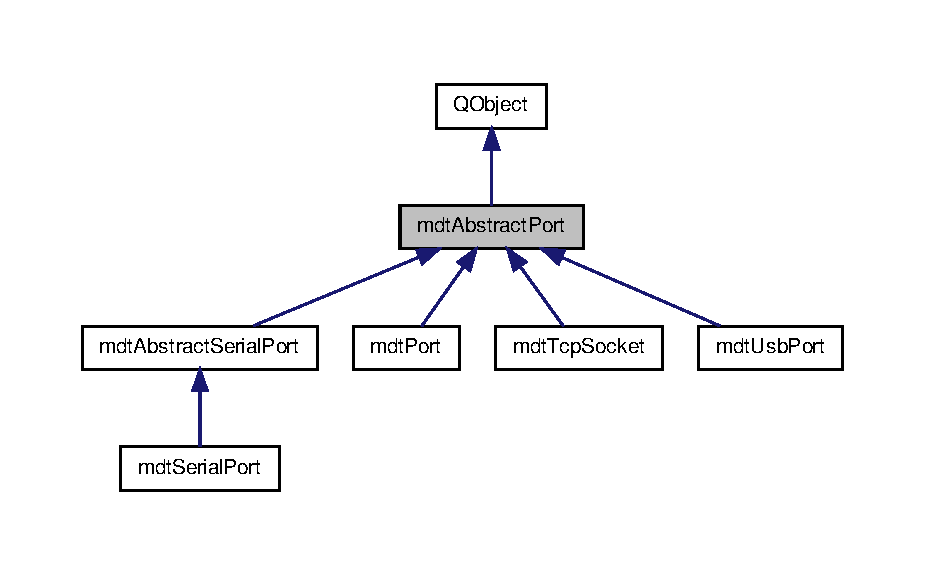
\includegraphics[width=400pt]{classmdt_abstract_port__inherit__graph}
\end{center}
\end{figure}


Collaboration diagram for mdtAbstractPort:\nopagebreak
\begin{figure}[H]
\begin{center}
\leavevmode
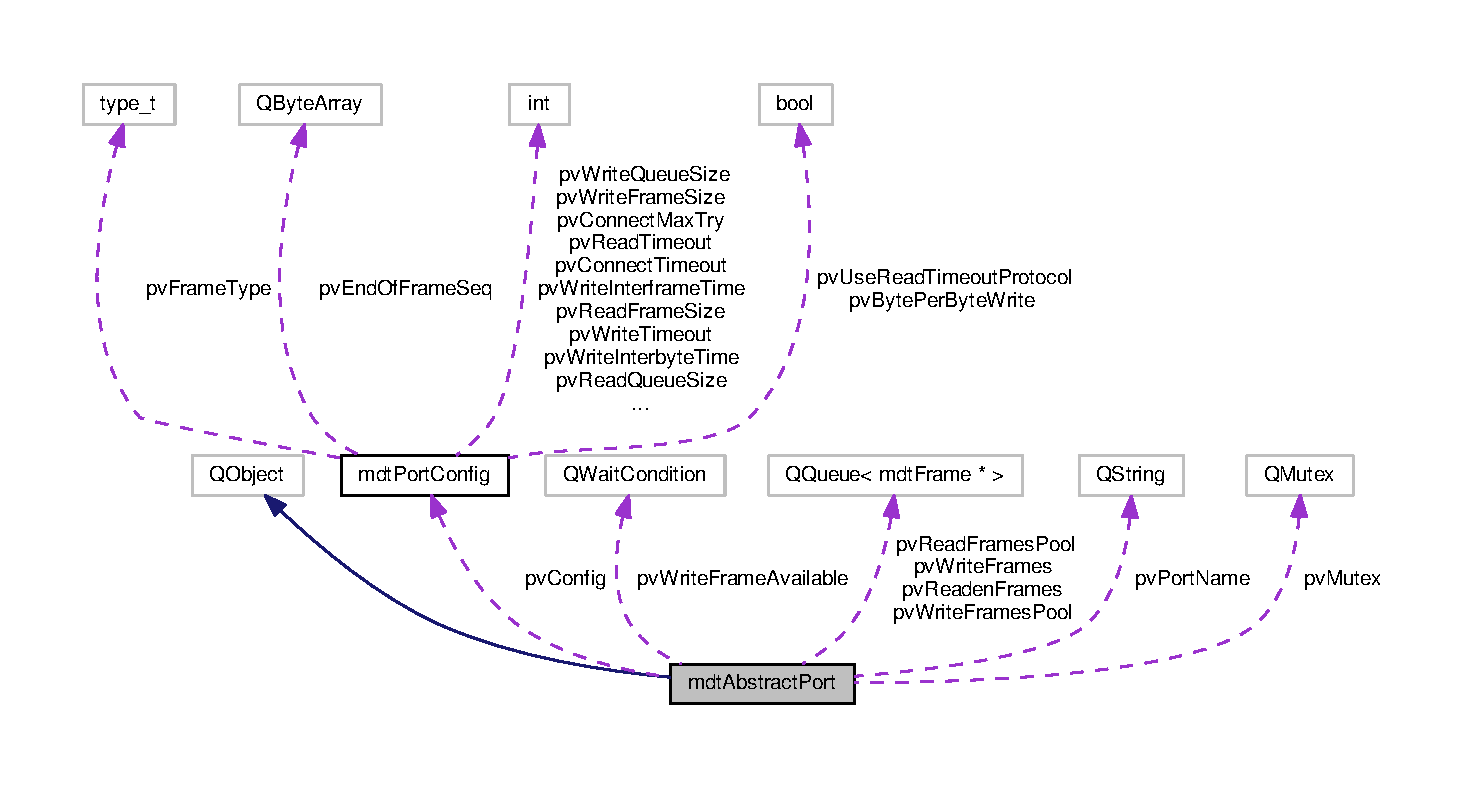
\includegraphics[width=168pt]{classmdt_abstract_port__coll__graph}
\end{center}
\end{figure}
\subsection*{Public Types}
\begin{DoxyCompactItemize}
\item 
enum \hyperlink{classmdt_abstract_port_ad4121bb930c95887e77f8bafa065a85e}{error\_\-t} \{ \par
\hyperlink{classmdt_abstract_port_ad4121bb930c95887e77f8bafa065a85eab898bd273effe5cb4ed1a399a2d4baad}{NoError} =  0, 
\hyperlink{classmdt_abstract_port_ad4121bb930c95887e77f8bafa065a85eaedd63daf0db75794bb8e8e467da9575c}{PortLocked}, 
\hyperlink{classmdt_abstract_port_ad4121bb930c95887e77f8bafa065a85ea54a896ba3ff98896390e87bfe1f29eb0}{PortNotFound}, 
\hyperlink{classmdt_abstract_port_ad4121bb930c95887e77f8bafa065a85eaee5a84e59e9dc5fcf27cac57068bb1f4}{PortAccess}, 
\par
\hyperlink{classmdt_abstract_port_ad4121bb930c95887e77f8bafa065a85ea3d692317af7125319f60204df3101307}{SetupError}, 
\hyperlink{classmdt_abstract_port_ad4121bb930c95887e77f8bafa065a85eacb8cc31d0b00dda9e25ed1cc1fa17871}{UnknownError}
 \}
\begin{DoxyCompactList}\small\item\em Error. \end{DoxyCompactList}\end{DoxyCompactItemize}
\subsection*{Signals}
\begin{DoxyCompactItemize}
\item 
\hypertarget{classmdt_abstract_port_a62c5e1f2beb6eddf740c8710ecb84ad1}{
void \hyperlink{classmdt_abstract_port_a62c5e1f2beb6eddf740c8710ecb84ad1}{readTimeoutStateChanged} (bool state)}
\label{classmdt_abstract_port_a62c5e1f2beb6eddf740c8710ecb84ad1}

\begin{DoxyCompactList}\small\item\em Emited when read timeout state changed. \end{DoxyCompactList}\item 
\hypertarget{classmdt_abstract_port_abd4a3e5738ac13167ddaafe95926ce4d}{
void \hyperlink{classmdt_abstract_port_abd4a3e5738ac13167ddaafe95926ce4d}{writeTimeoutStateChanged} (bool state)}
\label{classmdt_abstract_port_abd4a3e5738ac13167ddaafe95926ce4d}

\begin{DoxyCompactList}\small\item\em Emited when write timeout state changed. \end{DoxyCompactList}\end{DoxyCompactItemize}
\subsection*{Public Member Functions}
\begin{DoxyCompactItemize}
\item 
\hypertarget{classmdt_abstract_port_a35e7bff9413690833c832bf115da102f}{
{\bfseries mdtAbstractPort} (QObject $\ast$parent=0)}
\label{classmdt_abstract_port_a35e7bff9413690833c832bf115da102f}

\item 
virtual \hyperlink{classmdt_abstract_port_aa40baa0c593fef984f3796acafceee15}{$\sim$mdtAbstractPort} ()
\begin{DoxyCompactList}\small\item\em Destructor. \end{DoxyCompactList}\item 
void \hyperlink{classmdt_abstract_port_a0ca143d32fc677bac7c1cf0e04144932}{setPortName} (const QString \&portName)
\begin{DoxyCompactList}\small\item\em Set the port name. \end{DoxyCompactList}\item 
\hypertarget{classmdt_abstract_port_ac52fbd121f7cbb848a2f3e5d29fae615}{
QString \& \hyperlink{classmdt_abstract_port_ac52fbd121f7cbb848a2f3e5d29fae615}{portName} ()}
\label{classmdt_abstract_port_ac52fbd121f7cbb848a2f3e5d29fae615}

\begin{DoxyCompactList}\small\item\em Get port name. \end{DoxyCompactList}\item 
\hyperlink{classmdt_abstract_port_ad4121bb930c95887e77f8bafa065a85e}{error\_\-t} \hyperlink{classmdt_abstract_port_a4e0f0b7f9e24257677184e4bde10fdde}{open} ()
\begin{DoxyCompactList}\small\item\em Open the port given by \hyperlink{classmdt_abstract_port_a0ca143d32fc677bac7c1cf0e04144932}{setPortName()} \end{DoxyCompactList}\item 
\hypertarget{classmdt_abstract_port_a2122ae3141342ff38c8388e62b244e3b}{
bool \hyperlink{classmdt_abstract_port_a2122ae3141342ff38c8388e62b244e3b}{isOpen} () const }
\label{classmdt_abstract_port_a2122ae3141342ff38c8388e62b244e3b}

\begin{DoxyCompactList}\small\item\em Get port's open state. \end{DoxyCompactList}\item 
virtual void \hyperlink{classmdt_abstract_port_a1ace1a2bd1a04f16952980e247b04800}{close} ()
\begin{DoxyCompactList}\small\item\em Close the port. \end{DoxyCompactList}\item 
\hypertarget{classmdt_abstract_port_a48bdc0a8057c3b119763643098cf798f}{
void \hyperlink{classmdt_abstract_port_a48bdc0a8057c3b119763643098cf798f}{setConfig} (\hyperlink{classmdt_port_config}{mdtPortConfig} $\ast$cfg)}
\label{classmdt_abstract_port_a48bdc0a8057c3b119763643098cf798f}

\begin{DoxyCompactList}\small\item\em Set configuration. \end{DoxyCompactList}\item 
\hypertarget{classmdt_abstract_port_a3d105c90696f7c40f29c24fe9b6e4481}{
\hyperlink{classmdt_port_config}{mdtPortConfig} \& \hyperlink{classmdt_abstract_port_a3d105c90696f7c40f29c24fe9b6e4481}{config} ()}
\label{classmdt_abstract_port_a3d105c90696f7c40f29c24fe9b6e4481}

\begin{DoxyCompactList}\small\item\em Get the stored configuration. \end{DoxyCompactList}\item 
\hyperlink{classmdt_abstract_port_ad4121bb930c95887e77f8bafa065a85e}{error\_\-t} \hyperlink{classmdt_abstract_port_abc9f1154ac71c4e31ac3e7a3ff4c5182}{setup} ()
\begin{DoxyCompactList}\small\item\em Setup port with given configurations. \end{DoxyCompactList}\item 
virtual void \hyperlink{classmdt_abstract_port_a6589b04467e0073d18ba872201bdcd84}{setReadTimeout} (int timeout)=0
\begin{DoxyCompactList}\small\item\em Set the read data timeout. \end{DoxyCompactList}\item 
virtual void \hyperlink{classmdt_abstract_port_a12eb422d52ebb09a650f8497b258c2e7}{setWriteTimeout} (int timeout)=0
\begin{DoxyCompactList}\small\item\em Set the write data timeout. \end{DoxyCompactList}\item 
virtual bool \hyperlink{classmdt_abstract_port_a848e3c86aa6ec480e8c471655fbcf5c5}{waitForReadyRead} ()=0
\begin{DoxyCompactList}\small\item\em Wait until data is available on port. \end{DoxyCompactList}\item 
virtual bool \hyperlink{classmdt_abstract_port_a8a9177346624fb043689f1a5234fff4c}{waitForReadyRead} (\hyperlink{classmdt_port_thread}{mdtPortThread} $\ast$thread)
\begin{DoxyCompactList}\small\item\em NOTE: \end{DoxyCompactList}\item 
bool \hyperlink{classmdt_abstract_port_ae77785fbad938eac5f24f437e7683277}{waitForReadyRead} (int msecs)
\begin{DoxyCompactList}\small\item\em Wait until data is available on port. \end{DoxyCompactList}\item 
virtual qint64 \hyperlink{classmdt_abstract_port_a9d9c45220d5328c9856a2445557fe970}{read} (char $\ast$data, qint64 maxSize)=0
\begin{DoxyCompactList}\small\item\em Read data from port. \end{DoxyCompactList}\item 
virtual bool \hyperlink{classmdt_abstract_port_aff3d79248baf96e670eba6d2fef700b9}{suspendTransmission} ()
\begin{DoxyCompactList}\small\item\em Request to suspend transmission. \end{DoxyCompactList}\item 
virtual bool \hyperlink{classmdt_abstract_port_ad4a04c995df881593db0a309000be7a7}{resumeTransmission} ()
\begin{DoxyCompactList}\small\item\em Request to resume transmission. \end{DoxyCompactList}\item 
virtual void \hyperlink{classmdt_abstract_port_a32329b4188db796401e4f454755acb44}{flushIn} ()
\begin{DoxyCompactList}\small\item\em Flush read buffers. \end{DoxyCompactList}\item 
virtual void \hyperlink{classmdt_abstract_port_ab1738b5b6b78743ee2d36ccf5daa7c00}{readOneFrame} ()
\begin{DoxyCompactList}\small\item\em Just for special cases. \end{DoxyCompactList}\item 
virtual void \hyperlink{classmdt_abstract_port_a2235d62d9a9e4555d41773c41cc3bc70}{writeOneFrame} ()
\begin{DoxyCompactList}\small\item\em Just for special cases. \end{DoxyCompactList}\item 
virtual bool \hyperlink{classmdt_abstract_port_a7773bc21c63ce6a275f5a0889935ac83}{waitEventWriteReady} ()=0
\begin{DoxyCompactList}\small\item\em Wait until data can be written to port. \end{DoxyCompactList}\item 
virtual qint64 \hyperlink{classmdt_abstract_port_a64d4802975a76474b9196c91f57a6d90}{write} (const char $\ast$data, qint64 maxSize)=0
\begin{DoxyCompactList}\small\item\em Write data to port. \end{DoxyCompactList}\item 
virtual void \hyperlink{classmdt_abstract_port_ad199c6310801893f1f7de2a2391606fc}{flushOut} ()
\begin{DoxyCompactList}\small\item\em Flush write buffers. \end{DoxyCompactList}\item 
void \hyperlink{classmdt_abstract_port_a0fc7317e988d5dea53a999cd1bf4faa9}{updateReadTimeoutState} (bool state)
\begin{DoxyCompactList}\small\item\em Update the read timeout state. \end{DoxyCompactList}\item 
void \hyperlink{classmdt_abstract_port_ab51135de1f7bbc4707c3284f924c98dc}{updateWriteTimeoutState} (bool state)
\begin{DoxyCompactList}\small\item\em Update the write timeout state. \end{DoxyCompactList}\item 
bool \hyperlink{classmdt_abstract_port_aec94143165e486cbbe6e0979be887c7e}{readTimeoutOccured} ()
\begin{DoxyCompactList}\small\item\em Returns read timeout state. \end{DoxyCompactList}\item 
bool \hyperlink{classmdt_abstract_port_a7c05a1abe77f0c3c334016c6ad866f67}{writeTimeoutOccured} ()
\begin{DoxyCompactList}\small\item\em Returns write timeout state. \end{DoxyCompactList}\item 
void \hyperlink{classmdt_abstract_port_adf06d095d6c3e6ce939a3998bcf8b829}{initQueues} ()
\begin{DoxyCompactList}\small\item\em Init the read ans write queues. \end{DoxyCompactList}\item 
QQueue$<$ \hyperlink{classmdt_frame}{mdtFrame} $\ast$ $>$ \& \hyperlink{classmdt_abstract_port_a05356a33dc546a11d2794a0419d749e0}{readenFrames} ()
\begin{DoxyCompactList}\small\item\em Get the readen frames Queue. \end{DoxyCompactList}\item 
QQueue$<$ \hyperlink{classmdt_frame}{mdtFrame} $\ast$ $>$ \& \hyperlink{classmdt_abstract_port_a3850ab819a8fc5dad22af14b74c45274}{readFramesPool} ()
\begin{DoxyCompactList}\small\item\em Get the read frames Queue pool. \end{DoxyCompactList}\item 
QQueue$<$ \hyperlink{classmdt_frame}{mdtFrame} $\ast$ $>$ \& \hyperlink{classmdt_abstract_port_a4fed10be147dfce6ca315467ff3fb968}{writeFrames} ()
\begin{DoxyCompactList}\small\item\em Get the write frames Queue. \end{DoxyCompactList}\item 
QQueue$<$ \hyperlink{classmdt_frame}{mdtFrame} $\ast$ $>$ \& \hyperlink{classmdt_abstract_port_abf093b67fddebffa4f3c52277b9a8cf7}{writeFramesPool} ()
\begin{DoxyCompactList}\small\item\em Get the write frames Queue pool. \end{DoxyCompactList}\item 
\hypertarget{classmdt_abstract_port_a6bf2ecdcf894da3929a22eb8793a9fe3}{
void \hyperlink{classmdt_abstract_port_a6bf2ecdcf894da3929a22eb8793a9fe3}{lockMutex} ()}
\label{classmdt_abstract_port_a6bf2ecdcf894da3929a22eb8793a9fe3}

\begin{DoxyCompactList}\small\item\em Lock the mutex. \end{DoxyCompactList}\item 
\hypertarget{classmdt_abstract_port_a3523c72a06e4d950338f91e56c286e84}{
void \hyperlink{classmdt_abstract_port_a3523c72a06e4d950338f91e56c286e84}{unlockMutex} ()}
\label{classmdt_abstract_port_a3523c72a06e4d950338f91e56c286e84}

\begin{DoxyCompactList}\small\item\em Unlock the mutex. \end{DoxyCompactList}\end{DoxyCompactItemize}
\subsection*{Protected Member Functions}
\begin{DoxyCompactItemize}
\item 
virtual \hyperlink{classmdt_abstract_port_ad4121bb930c95887e77f8bafa065a85e}{error\_\-t} \hyperlink{classmdt_abstract_port_ac1440ea9759cbbee9efc5ea22afcdb0a}{pvOpen} ()=0
\begin{DoxyCompactList}\small\item\em Open the port given by \hyperlink{classmdt_abstract_port_a0ca143d32fc677bac7c1cf0e04144932}{setPortName()} \end{DoxyCompactList}\item 
virtual void \hyperlink{classmdt_abstract_port_add29e91ccc4be62ab5c0dcb2a68ae8f0}{pvClose} ()=0
\begin{DoxyCompactList}\small\item\em Close port. \end{DoxyCompactList}\item 
virtual \hyperlink{classmdt_abstract_port_ad4121bb930c95887e77f8bafa065a85e}{error\_\-t} \hyperlink{classmdt_abstract_port_a880e5ae1699af102f9a80501bb6a0021}{pvSetup} ()=0
\begin{DoxyCompactList}\small\item\em Setup port with given configurations. \end{DoxyCompactList}\end{DoxyCompactItemize}
\subsection*{Protected Attributes}
\begin{DoxyCompactItemize}
\item 
\hypertarget{classmdt_abstract_port_a9faa5966fcf4232b3d25034c0f67dd7c}{
bool {\bfseries pvReadTimeoutOccured}}
\label{classmdt_abstract_port_a9faa5966fcf4232b3d25034c0f67dd7c}

\item 
\hypertarget{classmdt_abstract_port_a2530e291d5ae4c1584595f9a5df7e9ff}{
bool {\bfseries pvReadTimeoutOccuredPrevious}}
\label{classmdt_abstract_port_a2530e291d5ae4c1584595f9a5df7e9ff}

\item 
\hypertarget{classmdt_abstract_port_ae5a003d280237700c8aa3cb6184e2d1b}{
bool {\bfseries pvWriteTimeoutOccured}}
\label{classmdt_abstract_port_ae5a003d280237700c8aa3cb6184e2d1b}

\item 
\hypertarget{classmdt_abstract_port_a8b65c0e26dc13147f02571ba74bef539}{
bool {\bfseries pvWriteTimeoutOccuredPrevious}}
\label{classmdt_abstract_port_a8b65c0e26dc13147f02571ba74bef539}

\item 
\hypertarget{classmdt_abstract_port_a412c3e4903bf7d90914cfeb273e82623}{
QQueue$<$ \hyperlink{classmdt_frame}{mdtFrame} $\ast$ $>$ {\bfseries pvReadenFrames}}
\label{classmdt_abstract_port_a412c3e4903bf7d90914cfeb273e82623}

\item 
\hypertarget{classmdt_abstract_port_a3d6bb9b420f64776d8fd077cf2b9b873}{
QQueue$<$ \hyperlink{classmdt_frame}{mdtFrame} $\ast$ $>$ {\bfseries pvReadFramesPool}}
\label{classmdt_abstract_port_a3d6bb9b420f64776d8fd077cf2b9b873}

\item 
\hypertarget{classmdt_abstract_port_a12cd5c1ba100b018539ed909a481d6dc}{
QQueue$<$ \hyperlink{classmdt_frame}{mdtFrame} $\ast$ $>$ {\bfseries pvWriteFrames}}
\label{classmdt_abstract_port_a12cd5c1ba100b018539ed909a481d6dc}

\item 
\hypertarget{classmdt_abstract_port_a67a8b1965f20a55ad115926aed0234b4}{
QQueue$<$ \hyperlink{classmdt_frame}{mdtFrame} $\ast$ $>$ {\bfseries pvWriteFramesPool}}
\label{classmdt_abstract_port_a67a8b1965f20a55ad115926aed0234b4}

\item 
\hypertarget{classmdt_abstract_port_a035d72bddbac47f405a8ecf0d2eeba66}{
\hyperlink{classmdt_port_config}{mdtPortConfig} $\ast$ {\bfseries pvConfig}}
\label{classmdt_abstract_port_a035d72bddbac47f405a8ecf0d2eeba66}

\item 
\hypertarget{classmdt_abstract_port_afb8f8a723ff2db5141f18750020a7ee9}{
QString {\bfseries pvPortName}}
\label{classmdt_abstract_port_afb8f8a723ff2db5141f18750020a7ee9}

\item 
\hypertarget{classmdt_abstract_port_a357bce65bc031fffa87090a26ab88a08}{
QMutex {\bfseries pvMutex}}
\label{classmdt_abstract_port_a357bce65bc031fffa87090a26ab88a08}

\end{DoxyCompactItemize}


\subsection{Detailed Description}
NOTE: file/port lock must be implemented ! (see Qt solution ? , sa: GtkTerm) 

Base class for port I/O 

\subsection{Member Enumeration Documentation}
\hypertarget{classmdt_abstract_port_ad4121bb930c95887e77f8bafa065a85e}{
\index{mdtAbstractPort@{mdtAbstractPort}!error\_\-t@{error\_\-t}}
\index{error\_\-t@{error\_\-t}!mdtAbstractPort@{mdtAbstractPort}}
\subsubsection[{error\_\-t}]{\setlength{\rightskip}{0pt plus 5cm}enum {\bf mdtAbstractPort::error\_\-t}}}
\label{classmdt_abstract_port_ad4121bb930c95887e77f8bafa065a85e}


Error. 

\begin{Desc}
\item[Enumerator: ]\par
\begin{description}
\index{NoError@{NoError}!mdtAbstractPort@{mdtAbstractPort}}\index{mdtAbstractPort@{mdtAbstractPort}!NoError@{NoError}}\item[{\em 
\hypertarget{classmdt_abstract_port_ad4121bb930c95887e77f8bafa065a85eab898bd273effe5cb4ed1a399a2d4baad}{
NoError}
\label{classmdt_abstract_port_ad4121bb930c95887e77f8bafa065a85eab898bd273effe5cb4ed1a399a2d4baad}
}]No error \index{PortLocked@{PortLocked}!mdtAbstractPort@{mdtAbstractPort}}\index{mdtAbstractPort@{mdtAbstractPort}!PortLocked@{PortLocked}}\item[{\em 
\hypertarget{classmdt_abstract_port_ad4121bb930c95887e77f8bafa065a85eaedd63daf0db75794bb8e8e467da9575c}{
PortLocked}
\label{classmdt_abstract_port_ad4121bb930c95887e77f8bafa065a85eaedd63daf0db75794bb8e8e467da9575c}
}]Port is allready locked \index{PortNotFound@{PortNotFound}!mdtAbstractPort@{mdtAbstractPort}}\index{mdtAbstractPort@{mdtAbstractPort}!PortNotFound@{PortNotFound}}\item[{\em 
\hypertarget{classmdt_abstract_port_ad4121bb930c95887e77f8bafa065a85ea54a896ba3ff98896390e87bfe1f29eb0}{
PortNotFound}
\label{classmdt_abstract_port_ad4121bb930c95887e77f8bafa065a85ea54a896ba3ff98896390e87bfe1f29eb0}
}]Port was not found \index{PortAccess@{PortAccess}!mdtAbstractPort@{mdtAbstractPort}}\index{mdtAbstractPort@{mdtAbstractPort}!PortAccess@{PortAccess}}\item[{\em 
\hypertarget{classmdt_abstract_port_ad4121bb930c95887e77f8bafa065a85eaee5a84e59e9dc5fcf27cac57068bb1f4}{
PortAccess}
\label{classmdt_abstract_port_ad4121bb930c95887e77f8bafa065a85eaee5a84e59e9dc5fcf27cac57068bb1f4}
}]Port cannot be open with requierd access (read, write) \index{SetupError@{SetupError}!mdtAbstractPort@{mdtAbstractPort}}\index{mdtAbstractPort@{mdtAbstractPort}!SetupError@{SetupError}}\item[{\em 
\hypertarget{classmdt_abstract_port_ad4121bb930c95887e77f8bafa065a85ea3d692317af7125319f60204df3101307}{
SetupError}
\label{classmdt_abstract_port_ad4121bb930c95887e77f8bafa065a85ea3d692317af7125319f60204df3101307}
}]Setup failed on a configuration option \index{UnknownError@{UnknownError}!mdtAbstractPort@{mdtAbstractPort}}\index{mdtAbstractPort@{mdtAbstractPort}!UnknownError@{UnknownError}}\item[{\em 
\hypertarget{classmdt_abstract_port_ad4121bb930c95887e77f8bafa065a85eacb8cc31d0b00dda9e25ed1cc1fa17871}{
UnknownError}
\label{classmdt_abstract_port_ad4121bb930c95887e77f8bafa065a85eacb8cc31d0b00dda9e25ed1cc1fa17871}
}]Unknown error is happen. Logfile could give more information, see \hyperlink{classmdt_error}{mdtError} and \hyperlink{classmdt_application}{mdtApplication} \end{description}
\end{Desc}



\subsection{Constructor \& Destructor Documentation}
\hypertarget{classmdt_abstract_port_aa40baa0c593fef984f3796acafceee15}{
\index{mdtAbstractPort@{mdtAbstractPort}!$\sim$mdtAbstractPort@{$\sim$mdtAbstractPort}}
\index{$\sim$mdtAbstractPort@{$\sim$mdtAbstractPort}!mdtAbstractPort@{mdtAbstractPort}}
\subsubsection[{$\sim$mdtAbstractPort}]{\setlength{\rightskip}{0pt plus 5cm}mdtAbstractPort::$\sim$mdtAbstractPort (
\begin{DoxyParamCaption}
{}
\end{DoxyParamCaption}
)\hspace{0.3cm}{\ttfamily  \mbox{[}virtual\mbox{]}}}}
\label{classmdt_abstract_port_aa40baa0c593fef984f3796acafceee15}


Destructor. 

Subclass notes:\par
 This destructor cannot call the \hyperlink{classmdt_abstract_port_a1ace1a2bd1a04f16952980e247b04800}{close()} method, because this will call the \hyperlink{classmdt_abstract_port_add29e91ccc4be62ab5c0dcb2a68ae8f0}{pvClose()} from destructed inherited object. So, the subclass must call \hyperlink{classmdt_abstract_port_a1ace1a2bd1a04f16952980e247b04800}{close()} in its own destructor. 

\subsection{Member Function Documentation}
\hypertarget{classmdt_abstract_port_a1ace1a2bd1a04f16952980e247b04800}{
\index{mdtAbstractPort@{mdtAbstractPort}!close@{close}}
\index{close@{close}!mdtAbstractPort@{mdtAbstractPort}}
\subsubsection[{close}]{\setlength{\rightskip}{0pt plus 5cm}void mdtAbstractPort::close (
\begin{DoxyParamCaption}
{}
\end{DoxyParamCaption}
)\hspace{0.3cm}{\ttfamily  \mbox{[}virtual\mbox{]}}}}
\label{classmdt_abstract_port_a1ace1a2bd1a04f16952980e247b04800}


Close the port. 

Close port if it is open.

The mutex is not handled by this method.

Subclass notes:\par
 Internally, this method calls \hyperlink{classmdt_abstract_port_add29e91ccc4be62ab5c0dcb2a68ae8f0}{pvClose()}. Once done, the flags are updated. Note that this method must be called from subclass destructor. See \hyperlink{classmdt_abstract_port_aa40baa0c593fef984f3796acafceee15}{$\sim$mdtAbstractPort()} for details.

\begin{Desc}
\item[\hyperlink{todo__todo000003}{Todo}]Actuellement, les queues sont deletée ici, que faire ? \end{Desc}


Reimplemented in \hyperlink{classmdt_abstract_serial_port_ae668910f98ad0e158dc6ebebf0c19805}{mdtAbstractSerialPort}.

\hypertarget{classmdt_abstract_port_a32329b4188db796401e4f454755acb44}{
\index{mdtAbstractPort@{mdtAbstractPort}!flushIn@{flushIn}}
\index{flushIn@{flushIn}!mdtAbstractPort@{mdtAbstractPort}}
\subsubsection[{flushIn}]{\setlength{\rightskip}{0pt plus 5cm}void mdtAbstractPort::flushIn (
\begin{DoxyParamCaption}
{}
\end{DoxyParamCaption}
)\hspace{0.3cm}{\ttfamily  \mbox{[}virtual\mbox{]}}}}
\label{classmdt_abstract_port_a32329b4188db796401e4f454755acb44}


Flush read buffers. 

Subclass notes:\par
 This method must be implemented in subclass.\par
 To handle port correctly, subclass must:
\begin{DoxyItemize}
\item Lock the mutex with \hyperlink{classmdt_abstract_port_a6bf2ecdcf894da3929a22eb8793a9fe3}{lockMutex()}
\item Call specific system flush function
\item Call this flush method ( with \hyperlink{classmdt_abstract_port_a32329b4188db796401e4f454755acb44}{mdtAbstractPort::flushIn()} ). The last step will move all pending frames to read pool.\par
 Note: if subclass has nothing to do it must lock the mutex and call this method. 
\end{DoxyItemize}

Reimplemented in \hyperlink{classmdt_port_a2fea088c8e5ad4578f521a39c353f7c3}{mdtPort}, and \hyperlink{classmdt_serial_port_a597d013bbe18b1f946b99f68a4856a87}{mdtSerialPort}.

\hypertarget{classmdt_abstract_port_ad199c6310801893f1f7de2a2391606fc}{
\index{mdtAbstractPort@{mdtAbstractPort}!flushOut@{flushOut}}
\index{flushOut@{flushOut}!mdtAbstractPort@{mdtAbstractPort}}
\subsubsection[{flushOut}]{\setlength{\rightskip}{0pt plus 5cm}void mdtAbstractPort::flushOut (
\begin{DoxyParamCaption}
{}
\end{DoxyParamCaption}
)\hspace{0.3cm}{\ttfamily  \mbox{[}virtual\mbox{]}}}}
\label{classmdt_abstract_port_ad199c6310801893f1f7de2a2391606fc}


Flush write buffers. 

Subclass notes:\par
 This method must be implemented in subclass.\par
 To handle port correctly, subclass must:
\begin{DoxyItemize}
\item Lock the mutex with \hyperlink{classmdt_abstract_port_a6bf2ecdcf894da3929a22eb8793a9fe3}{lockMutex()}
\item Call specific system flush function
\item Call this flush method ( with \hyperlink{classmdt_abstract_port_ad199c6310801893f1f7de2a2391606fc}{mdtAbstractPort::flushOut()} ). The last step will move all pending frames to read pool.\par
 Note: if subclass has nothing to do it must lock the mutex and call this method. 
\end{DoxyItemize}

Reimplemented in \hyperlink{classmdt_port_a42022f9fe08166418711b956c6aabb49}{mdtPort}, and \hyperlink{classmdt_serial_port_a3a446c34c9f98e0c14637ab3dcab98d0}{mdtSerialPort}.

\hypertarget{classmdt_abstract_port_adf06d095d6c3e6ce939a3998bcf8b829}{
\index{mdtAbstractPort@{mdtAbstractPort}!initQueues@{initQueues}}
\index{initQueues@{initQueues}!mdtAbstractPort@{mdtAbstractPort}}
\subsubsection[{initQueues}]{\setlength{\rightskip}{0pt plus 5cm}void mdtAbstractPort::initQueues (
\begin{DoxyParamCaption}
{}
\end{DoxyParamCaption}
)}}
\label{classmdt_abstract_port_adf06d095d6c3e6ce939a3998bcf8b829}


Init the read ans write queues. 

\begin{DoxyPrecond}{Precondition}
A valid configuration must be set before using this method. 
\end{DoxyPrecond}
\hypertarget{classmdt_abstract_port_a4e0f0b7f9e24257677184e4bde10fdde}{
\index{mdtAbstractPort@{mdtAbstractPort}!open@{open}}
\index{open@{open}!mdtAbstractPort@{mdtAbstractPort}}
\subsubsection[{open}]{\setlength{\rightskip}{0pt plus 5cm}{\bf mdtAbstractPort::error\_\-t} mdtAbstractPort::open (
\begin{DoxyParamCaption}
{}
\end{DoxyParamCaption}
)}}
\label{classmdt_abstract_port_a4e0f0b7f9e24257677184e4bde10fdde}


Open the port given by \hyperlink{classmdt_abstract_port_a0ca143d32fc677bac7c1cf0e04144932}{setPortName()} 

If port can be open successfull, NoError code is returned. If port is open, it will be closed first (by calling \hyperlink{classmdt_abstract_port_a1ace1a2bd1a04f16952980e247b04800}{close()}).

The mutex is not handled by this method.

Subclass notes:\par
 Internally, this method calls \hyperlink{classmdt_abstract_port_ac1440ea9759cbbee9efc5ea22afcdb0a}{pvOpen()}. Once done, the flags are updated.

\begin{DoxySeeAlso}{See also}
\hyperlink{classmdt_abstract_port_ad4121bb930c95887e77f8bafa065a85e}{error\_\-t} 
\end{DoxySeeAlso}
\hypertarget{classmdt_abstract_port_add29e91ccc4be62ab5c0dcb2a68ae8f0}{
\index{mdtAbstractPort@{mdtAbstractPort}!pvClose@{pvClose}}
\index{pvClose@{pvClose}!mdtAbstractPort@{mdtAbstractPort}}
\subsubsection[{pvClose}]{\setlength{\rightskip}{0pt plus 5cm}virtual void mdtAbstractPort::pvClose (
\begin{DoxyParamCaption}
{}
\end{DoxyParamCaption}
)\hspace{0.3cm}{\ttfamily  \mbox{[}protected, pure virtual\mbox{]}}}}
\label{classmdt_abstract_port_add29e91ccc4be62ab5c0dcb2a68ae8f0}


Close port. 

The mutex is not handled by this method.

\begin{DoxyPrecond}{Precondition}
The port must be open whenn calling this method.
\end{DoxyPrecond}
Subclass notes:\par
 This method must be re-\/implemented in subclass.\par
 To handle the port correctly, the subclass method must:
\begin{DoxyItemize}
\item Do the specific work. Note that port was open in exclusive mode. On Linux, don't forget to unlock the port with \hyperlink{classmdt_port_lock}{mdtPortLock}.
\item The \hyperlink{classmdt_error}{mdtError} system should be used (on error) to keep trace in logfile. 
\end{DoxyItemize}\hypertarget{classmdt_abstract_port_ac1440ea9759cbbee9efc5ea22afcdb0a}{
\index{mdtAbstractPort@{mdtAbstractPort}!pvOpen@{pvOpen}}
\index{pvOpen@{pvOpen}!mdtAbstractPort@{mdtAbstractPort}}
\subsubsection[{pvOpen}]{\setlength{\rightskip}{0pt plus 5cm}virtual {\bf error\_\-t} mdtAbstractPort::pvOpen (
\begin{DoxyParamCaption}
{}
\end{DoxyParamCaption}
)\hspace{0.3cm}{\ttfamily  \mbox{[}protected, pure virtual\mbox{]}}}}
\label{classmdt_abstract_port_ac1440ea9759cbbee9efc5ea22afcdb0a}


Open the port given by \hyperlink{classmdt_abstract_port_a0ca143d32fc677bac7c1cf0e04144932}{setPortName()} 

If port can be open successfull, NoError code is returned.

The mutex is not handled by this method.

\begin{DoxyPrecond}{Precondition}
The port must not be open whenn calling this method.
\end{DoxyPrecond}
Subclass notes:\par
 This method must be re-\/implemented in subclass.\par
 To handle the port correctly, the subclass method must:
\begin{DoxyItemize}
\item Do the specific work. Note that port must be open in exclusive mode. On Linux, the \hyperlink{classmdt_port_lock}{mdtPortLock} should be used for this.
\item The \hyperlink{classmdt_error}{mdtError} system should be used (on error) to keep trace in logfile.
\item If port must be closed (f.ex. on error), use the \hyperlink{classmdt_abstract_port_a1ace1a2bd1a04f16952980e247b04800}{close()} method to keep flags coherent.
\item Return the correct error code on failure (see the error\_\-t enum)
\end{DoxyItemize}

\begin{DoxySeeAlso}{See also}
\hyperlink{classmdt_abstract_port_a1ace1a2bd1a04f16952980e247b04800}{close()} 

\hyperlink{classmdt_abstract_port_ad4121bb930c95887e77f8bafa065a85e}{error\_\-t} 
\end{DoxySeeAlso}
\hypertarget{classmdt_abstract_port_a880e5ae1699af102f9a80501bb6a0021}{
\index{mdtAbstractPort@{mdtAbstractPort}!pvSetup@{pvSetup}}
\index{pvSetup@{pvSetup}!mdtAbstractPort@{mdtAbstractPort}}
\subsubsection[{pvSetup}]{\setlength{\rightskip}{0pt plus 5cm}virtual {\bf error\_\-t} mdtAbstractPort::pvSetup (
\begin{DoxyParamCaption}
{}
\end{DoxyParamCaption}
)\hspace{0.3cm}{\ttfamily  \mbox{[}protected, pure virtual\mbox{]}}}}
\label{classmdt_abstract_port_a880e5ae1699af102f9a80501bb6a0021}


Setup port with given configurations. 

The mutex is not handled by this method.

\begin{DoxyPrecond}{Precondition}
The port must be open whenn calling this method. 

A valid configuration must be set before calling this method.
\end{DoxyPrecond}
Subclass notes:\par
 This method must be re-\/implemented in subclass.\par
 To handle the port correctly, the subclass method must:
\begin{DoxyItemize}
\item Do the specific work
\item Set read/write timeouts using \hyperlink{classmdt_abstract_port_a6589b04467e0073d18ba872201bdcd84}{setReadTimeout()} and \hyperlink{classmdt_abstract_port_a12eb422d52ebb09a650f8497b258c2e7}{setWriteTimeout()}. See \hyperlink{classmdt_port_config}{mdtPortConfig} to know how to get these timeouts.
\item Return the correct error code on failure (see the error\_\-t enum)
\end{DoxyItemize}

Configuration is available using \hyperlink{classmdt_abstract_port_a3d105c90696f7c40f29c24fe9b6e4481}{config()}.

\begin{DoxySeeAlso}{See also}
\hyperlink{classmdt_abstract_port_ad4121bb930c95887e77f8bafa065a85e}{error\_\-t} 
\end{DoxySeeAlso}
\hypertarget{classmdt_abstract_port_a9d9c45220d5328c9856a2445557fe970}{
\index{mdtAbstractPort@{mdtAbstractPort}!read@{read}}
\index{read@{read}!mdtAbstractPort@{mdtAbstractPort}}
\subsubsection[{read}]{\setlength{\rightskip}{0pt plus 5cm}virtual qint64 mdtAbstractPort::read (
\begin{DoxyParamCaption}
\item[{char $\ast$}]{data, }
\item[{qint64}]{maxSize}
\end{DoxyParamCaption}
)\hspace{0.3cm}{\ttfamily  \mbox{[}pure virtual\mbox{]}}}}
\label{classmdt_abstract_port_a9d9c45220d5328c9856a2445557fe970}


Read data from port. 

This method is called from \hyperlink{classmdt_port_read_thread}{mdtPortReadThread} , and should not be used directly.

Subclass notes:\par
 This method must be implemented in subclass.\par
 Mutex is not handled by this method.

\begin{DoxyReturn}{Returns}
Number of bytes readen, or a error $<$ 0 
\end{DoxyReturn}


Implemented in \hyperlink{classmdt_port_ad8a196bb21b6ca76dffb068a1692904a}{mdtPort}, \hyperlink{classmdt_usbtmc_port_a91f45336ca9a71284e0309182f5e8ca1}{mdtUsbtmcPort}, \hyperlink{classmdt_tcp_socket_a78842bc5ddcac2d96fb368ee575214cd}{mdtTcpSocket}, and \hyperlink{classmdt_serial_port_a12274d7956b2af961ccdd36cfc2052cc}{mdtSerialPort}.

\hypertarget{classmdt_abstract_port_a05356a33dc546a11d2794a0419d749e0}{
\index{mdtAbstractPort@{mdtAbstractPort}!readenFrames@{readenFrames}}
\index{readenFrames@{readenFrames}!mdtAbstractPort@{mdtAbstractPort}}
\subsubsection[{readenFrames}]{\setlength{\rightskip}{0pt plus 5cm}QQueue$<$ {\bf mdtFrame} $\ast$ $>$ \& mdtAbstractPort::readenFrames (
\begin{DoxyParamCaption}
{}
\end{DoxyParamCaption}
)}}
\label{classmdt_abstract_port_a05356a33dc546a11d2794a0419d749e0}


Get the readen frames Queue. 

Readen frames queue contains frames that where received from device Note that the mutex is not handled by this method \hypertarget{classmdt_abstract_port_a3850ab819a8fc5dad22af14b74c45274}{
\index{mdtAbstractPort@{mdtAbstractPort}!readFramesPool@{readFramesPool}}
\index{readFramesPool@{readFramesPool}!mdtAbstractPort@{mdtAbstractPort}}
\subsubsection[{readFramesPool}]{\setlength{\rightskip}{0pt plus 5cm}QQueue$<$ {\bf mdtFrame} $\ast$ $>$ \& mdtAbstractPort::readFramesPool (
\begin{DoxyParamCaption}
{}
\end{DoxyParamCaption}
)}}
\label{classmdt_abstract_port_a3850ab819a8fc5dad22af14b74c45274}


Get the read frames Queue pool. 

Read frames queue pool contains frames that are ready to use for reception Note that the mutex is not handled by this method \hypertarget{classmdt_abstract_port_ab1738b5b6b78743ee2d36ccf5daa7c00}{
\index{mdtAbstractPort@{mdtAbstractPort}!readOneFrame@{readOneFrame}}
\index{readOneFrame@{readOneFrame}!mdtAbstractPort@{mdtAbstractPort}}
\subsubsection[{readOneFrame}]{\setlength{\rightskip}{0pt plus 5cm}void mdtAbstractPort::readOneFrame (
\begin{DoxyParamCaption}
{}
\end{DoxyParamCaption}
)\hspace{0.3cm}{\ttfamily  \mbox{[}virtual\mbox{]}}}}
\label{classmdt_abstract_port_ab1738b5b6b78743ee2d36ccf5daa7c00}


Just for special cases. 

In some case, this method is implemented in subclass. Default implementation does nothing. \begin{DoxySeeAlso}{See also}
\hyperlink{classmdt_usbtmc_port}{mdtUsbtmcPort} 
\end{DoxySeeAlso}


Reimplemented in \hyperlink{classmdt_usbtmc_port_a86ee5e17c32dea75e9f918389d3f7afc}{mdtUsbtmcPort}.

\hypertarget{classmdt_abstract_port_aec94143165e486cbbe6e0979be887c7e}{
\index{mdtAbstractPort@{mdtAbstractPort}!readTimeoutOccured@{readTimeoutOccured}}
\index{readTimeoutOccured@{readTimeoutOccured}!mdtAbstractPort@{mdtAbstractPort}}
\subsubsection[{readTimeoutOccured}]{\setlength{\rightskip}{0pt plus 5cm}bool mdtAbstractPort::readTimeoutOccured (
\begin{DoxyParamCaption}
{}
\end{DoxyParamCaption}
)}}
\label{classmdt_abstract_port_aec94143165e486cbbe6e0979be887c7e}


Returns read timeout state. 

Mutex is not handled by this method. \hypertarget{classmdt_abstract_port_ad4a04c995df881593db0a309000be7a7}{
\index{mdtAbstractPort@{mdtAbstractPort}!resumeTransmission@{resumeTransmission}}
\index{resumeTransmission@{resumeTransmission}!mdtAbstractPort@{mdtAbstractPort}}
\subsubsection[{resumeTransmission}]{\setlength{\rightskip}{0pt plus 5cm}bool mdtAbstractPort::resumeTransmission (
\begin{DoxyParamCaption}
{}
\end{DoxyParamCaption}
)\hspace{0.3cm}{\ttfamily  \mbox{[}virtual\mbox{]}}}}
\label{classmdt_abstract_port_ad4a04c995df881593db0a309000be7a7}


Request to resume transmission. 

This method is called from \hyperlink{classmdt_port_read_thread}{mdtPortReadThread} , and should not be used directly.\par
 Mutex is not handled by this method.

Subclass notes:\par
 This method must be implemented in subclass if requierd.\par
 Note about serial port subclass:\par
 the right flow control must be used regarding enabled flow control.\par
 Default implementation does nothing.\par


\begin{DoxyReturn}{Returns}
False on error, in this case, the reader thread will be stopped. 
\end{DoxyReturn}


Reimplemented in \hyperlink{classmdt_serial_port_a02fd5ee74a7f52c3bce0545ec8a659bf}{mdtSerialPort}.

\hypertarget{classmdt_abstract_port_a0ca143d32fc677bac7c1cf0e04144932}{
\index{mdtAbstractPort@{mdtAbstractPort}!setPortName@{setPortName}}
\index{setPortName@{setPortName}!mdtAbstractPort@{mdtAbstractPort}}
\subsubsection[{setPortName}]{\setlength{\rightskip}{0pt plus 5cm}void mdtAbstractPort::setPortName (
\begin{DoxyParamCaption}
\item[{const QString \&}]{portName}
\end{DoxyParamCaption}
)}}
\label{classmdt_abstract_port_a0ca143d32fc677bac7c1cf0e04144932}


Set the port name. 

Port name can be, f.ex. /dev/ttyS0 on Linux, or COM1 on Windows. This method just store given port name and does nothing else. \hypertarget{classmdt_abstract_port_a6589b04467e0073d18ba872201bdcd84}{
\index{mdtAbstractPort@{mdtAbstractPort}!setReadTimeout@{setReadTimeout}}
\index{setReadTimeout@{setReadTimeout}!mdtAbstractPort@{mdtAbstractPort}}
\subsubsection[{setReadTimeout}]{\setlength{\rightskip}{0pt plus 5cm}virtual void mdtAbstractPort::setReadTimeout (
\begin{DoxyParamCaption}
\item[{int}]{timeout}
\end{DoxyParamCaption}
)\hspace{0.3cm}{\ttfamily  \mbox{[}pure virtual\mbox{]}}}}
\label{classmdt_abstract_port_a6589b04467e0073d18ba872201bdcd84}


Set the read data timeout. 

Subclass notes:\par
 This method must be re-\/implemented in subclass. The subclass can convert and store the value in system specific type (f.ex: timeval struct on Posix) 
\begin{DoxyParams}{Parameters}
{\em timeout} & Timeout \mbox{[}ms\mbox{]} \\
\hline
\end{DoxyParams}


Implemented in \hyperlink{classmdt_port_aa77b266f23744f1b53ae589f986be101}{mdtPort}, \hyperlink{classmdt_usbtmc_port_ad3ec37dab7918fad36190b1c4c58c266}{mdtUsbtmcPort}, \hyperlink{classmdt_tcp_socket_aae23057f2e0ee326d0fee78ffe3f00f9}{mdtTcpSocket}, and \hyperlink{classmdt_serial_port_a9105e5a3a640b56097c1156000ace933}{mdtSerialPort}.

\hypertarget{classmdt_abstract_port_abc9f1154ac71c4e31ac3e7a3ff4c5182}{
\index{mdtAbstractPort@{mdtAbstractPort}!setup@{setup}}
\index{setup@{setup}!mdtAbstractPort@{mdtAbstractPort}}
\subsubsection[{setup}]{\setlength{\rightskip}{0pt plus 5cm}{\bf mdtAbstractPort::error\_\-t} mdtAbstractPort::setup (
\begin{DoxyParamCaption}
{}
\end{DoxyParamCaption}
)}}
\label{classmdt_abstract_port_abc9f1154ac71c4e31ac3e7a3ff4c5182}


Setup port with given configurations. 

If port is not open, \hyperlink{classmdt_abstract_port_a4e0f0b7f9e24257677184e4bde10fdde}{open()} will be called first. Then, \hyperlink{classmdt_abstract_port_a880e5ae1699af102f9a80501bb6a0021}{pvSetup()} is called, and finally queues initialized with \hyperlink{classmdt_abstract_port_adf06d095d6c3e6ce939a3998bcf8b829}{initQueues()}. If somethig fails, the port is closed again, and error code returned.

The mutex is not handled by this method.

\begin{DoxyPrecond}{Precondition}
A valid configuration must be set before calling this method.
\end{DoxyPrecond}
\begin{DoxySeeAlso}{See also}
\hyperlink{classmdt_abstract_port_ad4121bb930c95887e77f8bafa065a85e}{error\_\-t} 
\end{DoxySeeAlso}
\hypertarget{classmdt_abstract_port_a12eb422d52ebb09a650f8497b258c2e7}{
\index{mdtAbstractPort@{mdtAbstractPort}!setWriteTimeout@{setWriteTimeout}}
\index{setWriteTimeout@{setWriteTimeout}!mdtAbstractPort@{mdtAbstractPort}}
\subsubsection[{setWriteTimeout}]{\setlength{\rightskip}{0pt plus 5cm}virtual void mdtAbstractPort::setWriteTimeout (
\begin{DoxyParamCaption}
\item[{int}]{timeout}
\end{DoxyParamCaption}
)\hspace{0.3cm}{\ttfamily  \mbox{[}pure virtual\mbox{]}}}}
\label{classmdt_abstract_port_a12eb422d52ebb09a650f8497b258c2e7}


Set the write data timeout. 

Subclass notes:\par
 This method must be re-\/implemented in subclass. The subclass can convert and store the value in system specific type (f.ex: timeval struct on Posix) 
\begin{DoxyParams}{Parameters}
{\em timeout} & Timeout \mbox{[}ms\mbox{]} \\
\hline
\end{DoxyParams}


Implemented in \hyperlink{classmdt_port_a2acb6e7bedacdadf78ee735dc611abfa}{mdtPort}, \hyperlink{classmdt_usbtmc_port_a18ff8b76d07cd75339204f9389e1dd5c}{mdtUsbtmcPort}, \hyperlink{classmdt_tcp_socket_ac59d2dfdf405b5382f0f20d5b9f75fd0}{mdtTcpSocket}, and \hyperlink{classmdt_serial_port_a036f49d743838013c9a8cbf6a1dd40d1}{mdtSerialPort}.

\hypertarget{classmdt_abstract_port_aff3d79248baf96e670eba6d2fef700b9}{
\index{mdtAbstractPort@{mdtAbstractPort}!suspendTransmission@{suspendTransmission}}
\index{suspendTransmission@{suspendTransmission}!mdtAbstractPort@{mdtAbstractPort}}
\subsubsection[{suspendTransmission}]{\setlength{\rightskip}{0pt plus 5cm}bool mdtAbstractPort::suspendTransmission (
\begin{DoxyParamCaption}
{}
\end{DoxyParamCaption}
)\hspace{0.3cm}{\ttfamily  \mbox{[}virtual\mbox{]}}}}
\label{classmdt_abstract_port_aff3d79248baf96e670eba6d2fef700b9}


Request to suspend transmission. 

This method is called from \hyperlink{classmdt_port_read_thread}{mdtPortReadThread} , and should not be used directly.\par
 Mutex is not handled by this method.

Subclass notes:\par
 This method must be implemented in subclass if requierd.\par
 Note about serial port subclass:\par
 the right flow control must be used regarding enabled flow control.\par
 Default implementation does nothing.\par


\begin{DoxyReturn}{Returns}
False on error, in this case, the reader thread will be stopped. 
\end{DoxyReturn}


Reimplemented in \hyperlink{classmdt_serial_port_a9412faf413eca5ee3516139fdfaaf2fe}{mdtSerialPort}.

\hypertarget{classmdt_abstract_port_a0fc7317e988d5dea53a999cd1bf4faa9}{
\index{mdtAbstractPort@{mdtAbstractPort}!updateReadTimeoutState@{updateReadTimeoutState}}
\index{updateReadTimeoutState@{updateReadTimeoutState}!mdtAbstractPort@{mdtAbstractPort}}
\subsubsection[{updateReadTimeoutState}]{\setlength{\rightskip}{0pt plus 5cm}void mdtAbstractPort::updateReadTimeoutState (
\begin{DoxyParamCaption}
\item[{bool}]{state}
\end{DoxyParamCaption}
)}}
\label{classmdt_abstract_port_a0fc7317e988d5dea53a999cd1bf4faa9}


Update the read timeout state. 

This method must be called by system dependant waitEventRead() method. When the read timeout state chages, the signal \hyperlink{classmdt_abstract_port_a62c5e1f2beb6eddf740c8710ecb84ad1}{readTimeoutStateChanged()} is emited.\par
 Note: this method is called from \hyperlink{classmdt_port_read_thread}{mdtPortReadThread} , and should not be used directly\par
 Mutex is not handled by this method. \hypertarget{classmdt_abstract_port_ab51135de1f7bbc4707c3284f924c98dc}{
\index{mdtAbstractPort@{mdtAbstractPort}!updateWriteTimeoutState@{updateWriteTimeoutState}}
\index{updateWriteTimeoutState@{updateWriteTimeoutState}!mdtAbstractPort@{mdtAbstractPort}}
\subsubsection[{updateWriteTimeoutState}]{\setlength{\rightskip}{0pt plus 5cm}void mdtAbstractPort::updateWriteTimeoutState (
\begin{DoxyParamCaption}
\item[{bool}]{state}
\end{DoxyParamCaption}
)}}
\label{classmdt_abstract_port_ab51135de1f7bbc4707c3284f924c98dc}


Update the write timeout state. 

This method must be called by system dependant \hyperlink{classmdt_abstract_port_a7773bc21c63ce6a275f5a0889935ac83}{waitEventWriteReady()} method When the write timeout state chages, the signal \hyperlink{classmdt_abstract_port_abd4a3e5738ac13167ddaafe95926ce4d}{writeTimeoutStateChanged()} is emited.\par
 Note: this method is called from \hyperlink{classmdt_port_write_thread}{mdtPortWriteThread} , and should not be used directly\par
 Mutex is not handled by this method. \hypertarget{classmdt_abstract_port_a7773bc21c63ce6a275f5a0889935ac83}{
\index{mdtAbstractPort@{mdtAbstractPort}!waitEventWriteReady@{waitEventWriteReady}}
\index{waitEventWriteReady@{waitEventWriteReady}!mdtAbstractPort@{mdtAbstractPort}}
\subsubsection[{waitEventWriteReady}]{\setlength{\rightskip}{0pt plus 5cm}virtual bool mdtAbstractPort::waitEventWriteReady (
\begin{DoxyParamCaption}
{}
\end{DoxyParamCaption}
)\hspace{0.3cm}{\ttfamily  \mbox{[}pure virtual\mbox{]}}}}
\label{classmdt_abstract_port_a7773bc21c63ce6a275f5a0889935ac83}


Wait until data can be written to port. 

This method is called from \hyperlink{classmdt_port_write_thread}{mdtPortWriteThread} , and should not be used directly.\par
 Mutex must be locked before calling this method with \hyperlink{classmdt_abstract_port_a6bf2ecdcf894da3929a22eb8793a9fe3}{lockMutex()}. The mutex is locked when method returns.

Subclass notes:\par
 This method must be re-\/implemented in subclass.\par
 Notes about mutex handling:
\begin{DoxyItemize}
\item Mutex must be released during wait, and relocked befor return.
\end{DoxyItemize}

\begin{DoxyReturn}{Returns}
False on error, in this case, the reader thread will be stopped. 
\end{DoxyReturn}


Implemented in \hyperlink{classmdt_port_a2307bdc3b7d89f27e65b96b8a359b70a}{mdtPort}, \hyperlink{classmdt_usbtmc_port_aaa58100bc6ec2a5f91a3c6bb3676a468}{mdtUsbtmcPort}, \hyperlink{classmdt_tcp_socket_a91ada4fd18d31646c2a4d630b8f9ff21}{mdtTcpSocket}, and \hyperlink{classmdt_serial_port_a815275951e5834daf5068ffb48fcdcb3}{mdtSerialPort}.

\hypertarget{classmdt_abstract_port_a848e3c86aa6ec480e8c471655fbcf5c5}{
\index{mdtAbstractPort@{mdtAbstractPort}!waitForReadyRead@{waitForReadyRead}}
\index{waitForReadyRead@{waitForReadyRead}!mdtAbstractPort@{mdtAbstractPort}}
\subsubsection[{waitForReadyRead}]{\setlength{\rightskip}{0pt plus 5cm}virtual bool mdtAbstractPort::waitForReadyRead (
\begin{DoxyParamCaption}
{}
\end{DoxyParamCaption}
)\hspace{0.3cm}{\ttfamily  \mbox{[}pure virtual\mbox{]}}}}
\label{classmdt_abstract_port_a848e3c86aa6ec480e8c471655fbcf5c5}


Wait until data is available on port. 

This method is called from \hyperlink{classmdt_port_read_thread}{mdtPortReadThread} , and should not be used directly.\par
 Mutex must be locked before calling this method with \hyperlink{classmdt_abstract_port_a6bf2ecdcf894da3929a22eb8793a9fe3}{lockMutex()}. The mutex is locked when method returns.

Subclass notes:\par
 This method must be re-\/implemented in subclass. The read timeout state must be updated with \hyperlink{classmdt_abstract_port_a0fc7317e988d5dea53a999cd1bf4faa9}{updateReadTimeoutState()}\par
 Notes about mutex handling:
\begin{DoxyItemize}
\item Mutex must be released during wait, and relocked befor return.
\end{DoxyItemize}

\begin{DoxyReturn}{Returns}
False on error, in this case, the reader thread will emit errorOccured()
\end{DoxyReturn}
\begin{DoxySeeAlso}{See also}
\hyperlink{classmdt_port_thread}{mdtPortThread} 

\hyperlink{classmdt_port_config}{mdtPortConfig} 

\hyperlink{classmdt_tcp_socket_thread}{mdtTcpSocketThread} 
\end{DoxySeeAlso}


Implemented in \hyperlink{classmdt_port_af8737cc14667f6770af7be01759253e2}{mdtPort}, \hyperlink{classmdt_usbtmc_port_a46efba4f2d3dbb3c917368323de0333b}{mdtUsbtmcPort}, \hyperlink{classmdt_tcp_socket_a381bf5194cf180ca95f5f4bae730f73c}{mdtTcpSocket}, and \hyperlink{classmdt_serial_port_a0334aa073299f6161034e6be7c60939d}{mdtSerialPort}.

\hypertarget{classmdt_abstract_port_a8a9177346624fb043689f1a5234fff4c}{
\index{mdtAbstractPort@{mdtAbstractPort}!waitForReadyRead@{waitForReadyRead}}
\index{waitForReadyRead@{waitForReadyRead}!mdtAbstractPort@{mdtAbstractPort}}
\subsubsection[{waitForReadyRead}]{\setlength{\rightskip}{0pt plus 5cm}bool mdtAbstractPort::waitForReadyRead (
\begin{DoxyParamCaption}
\item[{{\bf mdtPortThread} $\ast$}]{thread}
\end{DoxyParamCaption}
)\hspace{0.3cm}{\ttfamily  \mbox{[}virtual\mbox{]}}}}
\label{classmdt_abstract_port_a8a9177346624fb043689f1a5234fff4c}


NOTE: 

NOTE: dummy method, to remove !!

\begin{Desc}
\item[\hyperlink{todo__todo000004}{Todo}]Comment, check, implement, remove this dummy implementation, move to pure virtual \end{Desc}
\hypertarget{classmdt_abstract_port_ae77785fbad938eac5f24f437e7683277}{
\index{mdtAbstractPort@{mdtAbstractPort}!waitForReadyRead@{waitForReadyRead}}
\index{waitForReadyRead@{waitForReadyRead}!mdtAbstractPort@{mdtAbstractPort}}
\subsubsection[{waitForReadyRead}]{\setlength{\rightskip}{0pt plus 5cm}bool mdtAbstractPort::waitForReadyRead (
\begin{DoxyParamCaption}
\item[{int}]{msecs}
\end{DoxyParamCaption}
)}}
\label{classmdt_abstract_port_ae77785fbad938eac5f24f437e7683277}


Wait until data is available on port. 

This method calls \hyperlink{classmdt_abstract_port_a6589b04467e0073d18ba872201bdcd84}{setReadTimeout()} and \hyperlink{classmdt_abstract_port_a848e3c86aa6ec480e8c471655fbcf5c5}{waitForReadyRead()} (it is a little bit slower than setting timeout one time, and call \hyperlink{classmdt_abstract_port_a848e3c86aa6ec480e8c471655fbcf5c5}{waitForReadyRead()} ).\par
 Note that the reader thread will call \hyperlink{classmdt_abstract_port_a848e3c86aa6ec480e8c471655fbcf5c5}{waitForReadyRead()} without argument.\par
 Note: this method is called from thread , and should not be used directly\par
 Mutex: see \hyperlink{classmdt_abstract_port_a848e3c86aa6ec480e8c471655fbcf5c5}{waitForReadyRead()} \begin{DoxyReturn}{Returns}
False on error, in this case, the reader thread will be stopped. 
\end{DoxyReturn}
\begin{DoxySeeAlso}{See also}
\hyperlink{classmdt_abstract_port_a848e3c86aa6ec480e8c471655fbcf5c5}{waitForReadyRead()} 
\end{DoxySeeAlso}
\hypertarget{classmdt_abstract_port_a64d4802975a76474b9196c91f57a6d90}{
\index{mdtAbstractPort@{mdtAbstractPort}!write@{write}}
\index{write@{write}!mdtAbstractPort@{mdtAbstractPort}}
\subsubsection[{write}]{\setlength{\rightskip}{0pt plus 5cm}virtual qint64 mdtAbstractPort::write (
\begin{DoxyParamCaption}
\item[{const char $\ast$}]{data, }
\item[{qint64}]{maxSize}
\end{DoxyParamCaption}
)\hspace{0.3cm}{\ttfamily  \mbox{[}pure virtual\mbox{]}}}}
\label{classmdt_abstract_port_a64d4802975a76474b9196c91f57a6d90}


Write data to port. 

This method is called from \hyperlink{classmdt_port_write_thread}{mdtPortWriteThread} , and should not be used directly. Mutex is not handled by this method.

Subclass notes:\par
 This method must be implemented in subclass.\par


\begin{DoxyReturn}{Returns}
Number of bytes written, or $<$0 on error 
\end{DoxyReturn}


Implemented in \hyperlink{classmdt_port_a62f4a6f2c547d40d3743ce893e0f64d6}{mdtPort}, \hyperlink{classmdt_usbtmc_port_a32b98d2a61617293c328a343d62d52c3}{mdtUsbtmcPort}, \hyperlink{classmdt_tcp_socket_adbf2db44b291127a499d9f8720beb632}{mdtTcpSocket}, and \hyperlink{classmdt_serial_port_a282f99035c032fbb6fa86ccd10deb597}{mdtSerialPort}.

\hypertarget{classmdt_abstract_port_a4fed10be147dfce6ca315467ff3fb968}{
\index{mdtAbstractPort@{mdtAbstractPort}!writeFrames@{writeFrames}}
\index{writeFrames@{writeFrames}!mdtAbstractPort@{mdtAbstractPort}}
\subsubsection[{writeFrames}]{\setlength{\rightskip}{0pt plus 5cm}QQueue$<$ {\bf mdtFrame} $\ast$ $>$ \& mdtAbstractPort::writeFrames (
\begin{DoxyParamCaption}
{}
\end{DoxyParamCaption}
)}}
\label{classmdt_abstract_port_a4fed10be147dfce6ca315467ff3fb968}


Get the write frames Queue. 

Write frames queue contains frames that must be sent Note that the mutex is not handled by this method \hypertarget{classmdt_abstract_port_abf093b67fddebffa4f3c52277b9a8cf7}{
\index{mdtAbstractPort@{mdtAbstractPort}!writeFramesPool@{writeFramesPool}}
\index{writeFramesPool@{writeFramesPool}!mdtAbstractPort@{mdtAbstractPort}}
\subsubsection[{writeFramesPool}]{\setlength{\rightskip}{0pt plus 5cm}QQueue$<$ {\bf mdtFrame} $\ast$ $>$ \& mdtAbstractPort::writeFramesPool (
\begin{DoxyParamCaption}
{}
\end{DoxyParamCaption}
)}}
\label{classmdt_abstract_port_abf093b67fddebffa4f3c52277b9a8cf7}


Get the write frames Queue pool. 

Write frames queue pool contains frames that are ready to use for transmission Note that serialPort mutex is not handled by this method \hypertarget{classmdt_abstract_port_a2235d62d9a9e4555d41773c41cc3bc70}{
\index{mdtAbstractPort@{mdtAbstractPort}!writeOneFrame@{writeOneFrame}}
\index{writeOneFrame@{writeOneFrame}!mdtAbstractPort@{mdtAbstractPort}}
\subsubsection[{writeOneFrame}]{\setlength{\rightskip}{0pt plus 5cm}void mdtAbstractPort::writeOneFrame (
\begin{DoxyParamCaption}
{}
\end{DoxyParamCaption}
)\hspace{0.3cm}{\ttfamily  \mbox{[}virtual\mbox{]}}}}
\label{classmdt_abstract_port_a2235d62d9a9e4555d41773c41cc3bc70}


Just for special cases. 

In some case, this method is implemented in subclass. Default implementation does nothing. \begin{DoxySeeAlso}{See also}
\hyperlink{classmdt_usbtmc_port}{mdtUsbtmcPort} 
\end{DoxySeeAlso}


Reimplemented in \hyperlink{classmdt_usbtmc_port_a97fca5f136f232275d90ab5b8c5ce285}{mdtUsbtmcPort}.

\hypertarget{classmdt_abstract_port_a7c05a1abe77f0c3c334016c6ad866f67}{
\index{mdtAbstractPort@{mdtAbstractPort}!writeTimeoutOccured@{writeTimeoutOccured}}
\index{writeTimeoutOccured@{writeTimeoutOccured}!mdtAbstractPort@{mdtAbstractPort}}
\subsubsection[{writeTimeoutOccured}]{\setlength{\rightskip}{0pt plus 5cm}bool mdtAbstractPort::writeTimeoutOccured (
\begin{DoxyParamCaption}
{}
\end{DoxyParamCaption}
)}}
\label{classmdt_abstract_port_a7c05a1abe77f0c3c334016c6ad866f67}


Returns write timeout state. 

Mutex is not handled by this method. 

The documentation for this class was generated from the following files:\begin{DoxyCompactItemize}
\item 
src/mdtport/mdtAbstractPort.h\item 
src/mdtport/mdtAbstractPort.cpp\item 
src/mdtport/moc\_\-mdtAbstractPort.cxx\end{DoxyCompactItemize}

\hypertarget{classmdt_abstract_serial_port}{\section{mdt\-Abstract\-Serial\-Port Class Reference}
\label{classmdt_abstract_serial_port}\index{mdt\-Abstract\-Serial\-Port@{mdt\-Abstract\-Serial\-Port}}
}


N\-O\-T\-E\-:  




{\ttfamily \#include $<$mdt\-Abstract\-Serial\-Port.\-h$>$}



Inheritance diagram for mdt\-Abstract\-Serial\-Port\-:\nopagebreak
\begin{figure}[H]
\begin{center}
\leavevmode
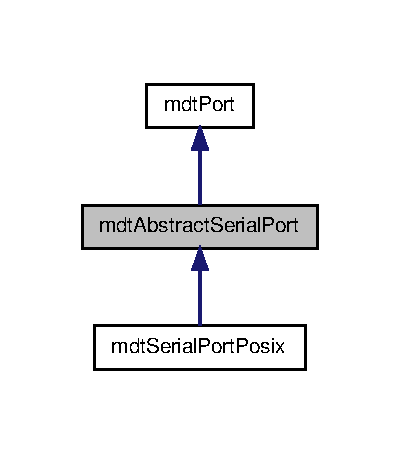
\includegraphics[width=192pt]{classmdt_abstract_serial_port__inherit__graph}
\end{center}
\end{figure}


Collaboration diagram for mdt\-Abstract\-Serial\-Port\-:\nopagebreak
\begin{figure}[H]
\begin{center}
\leavevmode
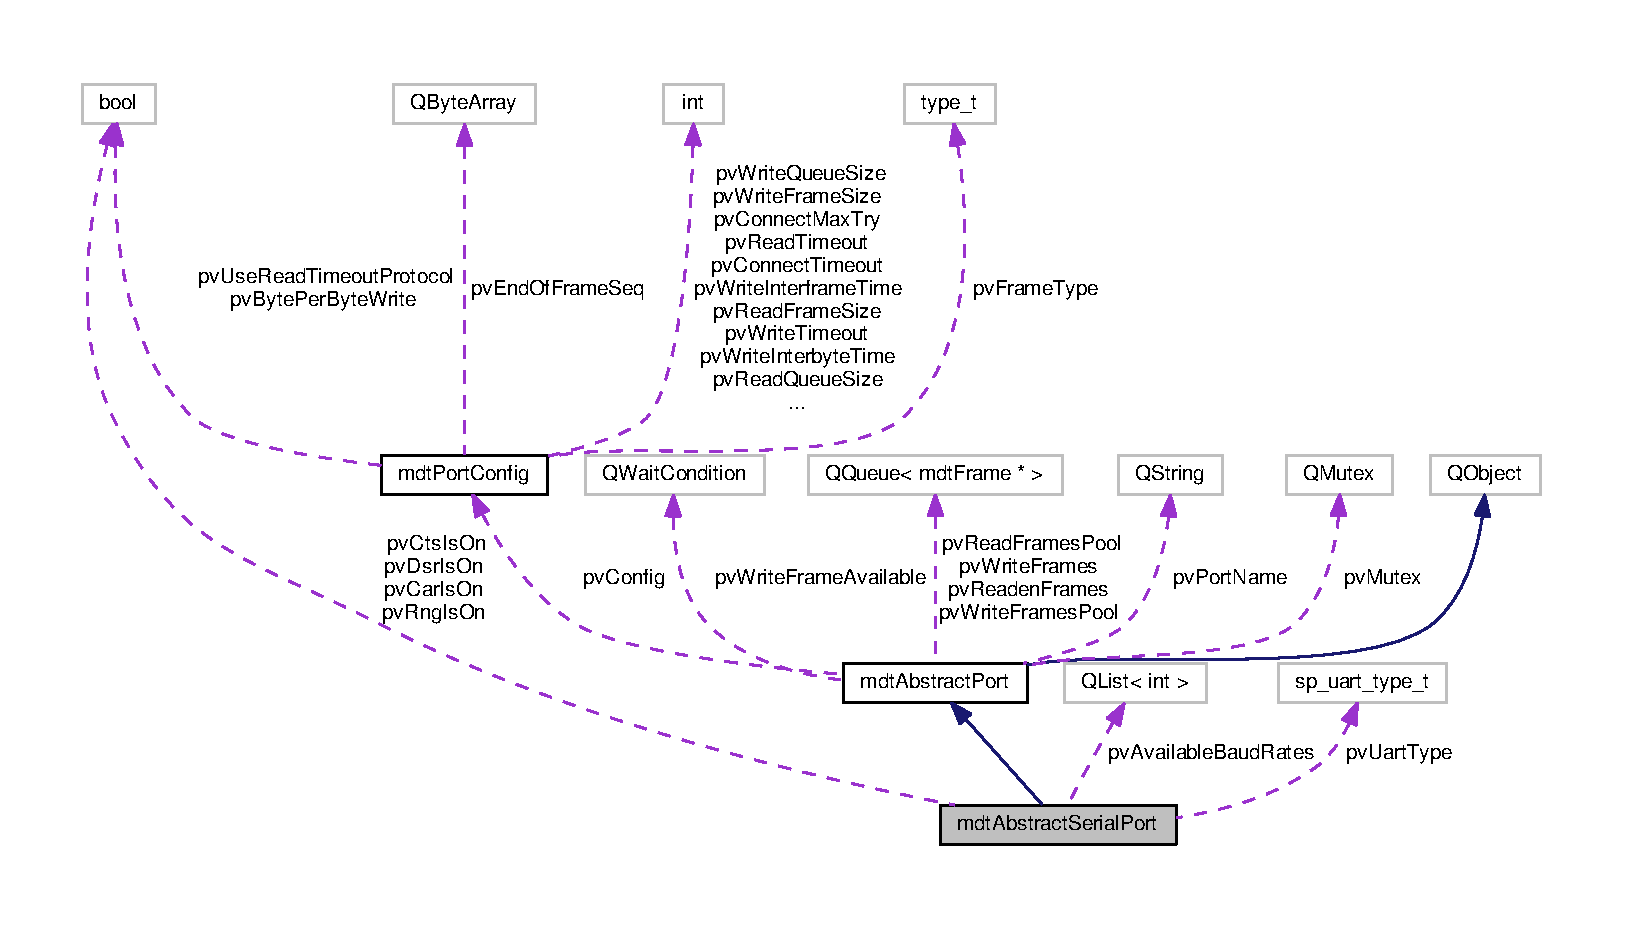
\includegraphics[width=350pt]{classmdt_abstract_serial_port__coll__graph}
\end{center}
\end{figure}
\subsection*{Public Types}
\begin{DoxyCompactItemize}
\item 
enum \hyperlink{classmdt_abstract_serial_port_a56b107c57fb0acb17cfcca262abe6a54}{sp\-\_\-uart\-\_\-type\-\_\-t} \{ \\*
\hyperlink{classmdt_abstract_serial_port_a56b107c57fb0acb17cfcca262abe6a54aee11b58fe38044177836f8dee7a56856}{U\-T\-\_\-\-U\-N\-K\-N\-O\-W}, 
\hyperlink{classmdt_abstract_serial_port_a56b107c57fb0acb17cfcca262abe6a54adad952850d3c9dacf0702f50dd35b6c3}{U\-T\-\_\-8250}, 
\hyperlink{classmdt_abstract_serial_port_a56b107c57fb0acb17cfcca262abe6a54aa83713734fb6f673c37476c47b4f9f72}{U\-T\-\_\-16450}, 
\hyperlink{classmdt_abstract_serial_port_a56b107c57fb0acb17cfcca262abe6a54a7c917ddd07b0e07cfa15719a9ea25c8c}{U\-T\-\_\-16550}, 
\\*
\hyperlink{classmdt_abstract_serial_port_a56b107c57fb0acb17cfcca262abe6a54a6022c299ae8e83784417d9177436b7cf}{U\-T\-\_\-16550\-A}, 
\hyperlink{classmdt_abstract_serial_port_a56b107c57fb0acb17cfcca262abe6a54a2bcb8cbd59857f3c30f31bf58725d702}{U\-T\-\_\-\-C\-I\-R\-R\-U\-S}, 
\hyperlink{classmdt_abstract_serial_port_a56b107c57fb0acb17cfcca262abe6a54aae40e02ba754679e05c5f724947e81c4}{U\-T\-\_\-16650}, 
\hyperlink{classmdt_abstract_serial_port_a56b107c57fb0acb17cfcca262abe6a54a78053265ac2720e1fd1b7a2aff6ff88f}{U\-T\-\_\-16650\-V2}, 
\\*
\hyperlink{classmdt_abstract_serial_port_a56b107c57fb0acb17cfcca262abe6a54ac5ef0346fc6f75a5c1c0a17eefd93377}{U\-T\-\_\-16750}, 
\hyperlink{classmdt_abstract_serial_port_a56b107c57fb0acb17cfcca262abe6a54ad938f46997e71ad974bc60effc58c915}{U\-T\-\_\-\-S\-T\-A\-R\-T\-E\-C\-H}, 
\hyperlink{classmdt_abstract_serial_port_a56b107c57fb0acb17cfcca262abe6a54ae5b8b4d0daf8047af55c4e794111725b}{U\-T\-\_\-16\-C950}, 
\hyperlink{classmdt_abstract_serial_port_a56b107c57fb0acb17cfcca262abe6a54ad764942882657984584696f6e43472ab}{U\-T\-\_\-16654}, 
\\*
\hyperlink{classmdt_abstract_serial_port_a56b107c57fb0acb17cfcca262abe6a54aaa3d3889f3880188393d6aa5769cd3af}{U\-T\-\_\-16850}, 
\hyperlink{classmdt_abstract_serial_port_a56b107c57fb0acb17cfcca262abe6a54afca5a97b8ebc740e56d24590c59ef19b}{U\-T\-\_\-\-R\-S\-A}
 \}
\begin{DoxyCompactList}\small\item\em U\-A\-R\-T type. \end{DoxyCompactList}\end{DoxyCompactItemize}
\subsection*{Public Slots}
\begin{DoxyCompactItemize}
\item 
virtual void \hyperlink{classmdt_abstract_serial_port_a0ef2426fbd1afbcb0701f327cc16a7cc}{set\-Rts} (bool on)=0
\begin{DoxyCompactList}\small\item\em Enable/diseable the R\-T\-S (Request To Send) signal. \end{DoxyCompactList}\item 
virtual void \hyperlink{classmdt_abstract_serial_port_aa86a8bc0bb03ac2b07bf43968dfeb189}{set\-Dtr} (bool on)=0
\begin{DoxyCompactList}\small\item\em Enable/diseable the D\-T\-R (Data Terminal Ready) signal. \end{DoxyCompactList}\end{DoxyCompactItemize}
\subsection*{Signals}
\begin{DoxyCompactItemize}
\item 
void \hyperlink{classmdt_abstract_serial_port_a63ddcadf5d8a63c479b0b6a24f89c837}{car\-Changed} (bool on)
\begin{DoxyCompactList}\small\item\em Emited whenn C\-A\-R (C\-D) status changed. \end{DoxyCompactList}\item 
void \hyperlink{classmdt_abstract_serial_port_a077d8c39ed12713742f1f2ffa0dca11d}{dsr\-Changed} (bool on)
\begin{DoxyCompactList}\small\item\em Emited whenn D\-S\-R status changed. \end{DoxyCompactList}\item 
void \hyperlink{classmdt_abstract_serial_port_adf45a5006218ef5660721ecdf8454b5d}{cts\-Changed} (bool on)
\begin{DoxyCompactList}\small\item\em Emited whenn C\-T\-S status changed. \end{DoxyCompactList}\item 
void \hyperlink{classmdt_abstract_serial_port_a47c08ccb99dc6de76ae58ebeefc26857}{rng\-Changed} (bool on)
\begin{DoxyCompactList}\small\item\em Emited whenn R\-N\-G (R\-I) status changed. \end{DoxyCompactList}\end{DoxyCompactItemize}
\subsection*{Public Member Functions}
\begin{DoxyCompactItemize}
\item 
\hyperlink{classmdt_abstract_serial_port_ae379b6151edebc1518e81ec061e379db}{mdt\-Abstract\-Serial\-Port} (\hyperlink{class_q_object}{Q\-Object} $\ast$parent=0)
\item 
virtual \hyperlink{classmdt_abstract_serial_port_af695a8df8e155a938da8e7bd00e34631}{$\sim$mdt\-Abstract\-Serial\-Port} ()
\item 
void \hyperlink{classmdt_abstract_serial_port_ae668910f98ad0e158dc6ebebf0c19805}{close} ()
\begin{DoxyCompactList}\small\item\em Close the serial port. \end{DoxyCompactList}\item 
\hyperlink{classmdt_serial_port_config}{mdt\-Serial\-Port\-Config} \& \hyperlink{classmdt_abstract_serial_port_ae053b73fee897769641813df658c9ead}{config} ()
\begin{DoxyCompactList}\small\item\em Get the stored configuration. \end{DoxyCompactList}\item 
\hyperlink{classmdt_abstract_serial_port_a56b107c57fb0acb17cfcca262abe6a54}{sp\-\_\-uart\-\_\-type\-\_\-t} \hyperlink{classmdt_abstract_serial_port_a6b153155d9e110336d51ec48d2cee203}{uart\-Type} ()
\begin{DoxyCompactList}\small\item\em Get U\-A\-R\-T type. \end{DoxyCompactList}\item 
Q\-String \hyperlink{classmdt_abstract_serial_port_a669c9ce68455abd3cfdb98259996e701}{uart\-Type\-Str} ()
\item 
Q\-List$<$ int $>$ \& \hyperlink{classmdt_abstract_serial_port_aecd76bff0f93cb86c3bbfd73e3776032}{available\-Baud\-Rates} ()
\begin{DoxyCompactList}\small\item\em Get the list of available baud rates. \end{DoxyCompactList}\item 
virtual bool \hyperlink{classmdt_abstract_serial_port_ae250b30c1db5652bd2abe2caf1c9d5c7}{set\-Baud\-Rate} (int rate)=0
\begin{DoxyCompactList}\small\item\em Set the baud rate. \end{DoxyCompactList}\item 
virtual int \hyperlink{classmdt_abstract_serial_port_ad9f5b7e939c60cd3766d2bf76df4af4b}{baud\-Rate} ()=0
\begin{DoxyCompactList}\small\item\em Get the baud rate. \end{DoxyCompactList}\item 
virtual bool \hyperlink{classmdt_abstract_serial_port_a323e590d6ead87033985ffff1ecfae81}{set\-Data\-Bits} (int n)=0
\begin{DoxyCompactList}\small\item\em Set number of data bits. \end{DoxyCompactList}\item 
virtual int \hyperlink{classmdt_abstract_serial_port_a63e2a14c416d9c3516ec74f5e37f4cc7}{data\-Bits} ()=0
\begin{DoxyCompactList}\small\item\em Get number of data bits. \end{DoxyCompactList}\item 
virtual bool \hyperlink{classmdt_abstract_serial_port_a164c7be802a04805e5b401fc5011208b}{set\-Stop\-Bits} (int n)=0
\begin{DoxyCompactList}\small\item\em Set number of stop bits. \end{DoxyCompactList}\item 
virtual int \hyperlink{classmdt_abstract_serial_port_abae48c24634c3e2d298f1cff98b250ed}{stop\-Bits} ()=0
\begin{DoxyCompactList}\small\item\em Get number of stop bits. \end{DoxyCompactList}\item 
virtual bool \hyperlink{classmdt_abstract_serial_port_ac9c6990ac9861f21dcfe27c989b78545}{set\-Parity} (\hyperlink{classmdt_serial_port_config_a4b9e444637cf0193a125fabdd67d8bfe}{mdt\-Serial\-Port\-Config\-::parity\-\_\-t} p)=0
\begin{DoxyCompactList}\small\item\em Set parity check. \end{DoxyCompactList}\item 
virtual \\*
\hyperlink{classmdt_serial_port_config_a4b9e444637cf0193a125fabdd67d8bfe}{mdt\-Serial\-Port\-Config\-::parity\-\_\-t} \hyperlink{classmdt_abstract_serial_port_ac361191b58789065fcea742019b958f9}{parity} ()=0
\begin{DoxyCompactList}\small\item\em Get configured parity. \end{DoxyCompactList}\item 
virtual bool \hyperlink{classmdt_abstract_serial_port_af01806f53cfc5ef90b34c0645cee3bdf}{set\-Flow\-Ctl\-Rts\-Cts} (bool on)=0
\begin{DoxyCompactList}\small\item\em Enable/diseable R\-T\-S/\-C\-T\-S flow control. \end{DoxyCompactList}\item 
virtual bool \hyperlink{classmdt_abstract_serial_port_a7a1163b4d44d80369bd56c65af7942ad}{flow\-Ctl\-Rts\-Cts\-On} ()=0
\begin{DoxyCompactList}\small\item\em Get configured state of R\-T\-S/\-C\-T\-S flow control. \end{DoxyCompactList}\item 
virtual bool \hyperlink{classmdt_abstract_serial_port_a05b35143f7b048ebcb2295fdc2ac5013}{set\-Flow\-Ctl\-Xon\-Xoff} (bool on, char xon\-Char, char xoff\-Char)=0
\begin{DoxyCompactList}\small\item\em Enable/diseable Xon/\-Xoff flow control. \end{DoxyCompactList}\item 
virtual bool \hyperlink{classmdt_abstract_serial_port_a80074ba4e5bf44c3e2aebb82214499ee}{flow\-Ctl\-Xon\-Xoff\-On} ()=0
\begin{DoxyCompactList}\small\item\em Get configured state of Xon/\-Xoff flow control. \end{DoxyCompactList}\item 
virtual \hyperlink{classmdt_abstract_port_ad4121bb930c95887e77f8bafa065a85e}{error\-\_\-t} \hyperlink{classmdt_abstract_serial_port_a146bf17f4f11c173e9b123bace0f2ddf}{wait\-Event\-Ctl} ()=0
\begin{DoxyCompactList}\small\item\em Wait until a control (modem line) signal state changes. \end{DoxyCompactList}\item 
virtual bool \hyperlink{classmdt_abstract_serial_port_aaeacd26b220ab0f8c521cef74edfafdd}{get\-Ctl\-States} ()=0
\begin{DoxyCompactList}\small\item\em N\-O\-T\-E\-: \end{DoxyCompactList}\item 
bool \hyperlink{classmdt_abstract_serial_port_abf0be424c1a8cf01b830cc6b371e8695}{car\-Is\-On} ()
\begin{DoxyCompactList}\small\item\em Get the C\-A\-R (C\-D) state. \end{DoxyCompactList}\item 
bool \hyperlink{classmdt_abstract_serial_port_a76816aa53a6dce0ab30b9f1d095dd045}{dsr\-Is\-On} ()
\begin{DoxyCompactList}\small\item\em Get the D\-S\-R state. \end{DoxyCompactList}\item 
bool \hyperlink{classmdt_abstract_serial_port_a9bea314eefd6f4ec79456bc21e6c66af}{cts\-Is\-On} ()
\begin{DoxyCompactList}\small\item\em Get the C\-T\-S state. \end{DoxyCompactList}\item 
bool \hyperlink{classmdt_abstract_serial_port_a0a3954438d1e8180e53717cc0fe1ce3e}{rng\-Is\-On} ()
\begin{DoxyCompactList}\small\item\em Get the R\-N\-G (R\-I) state. \end{DoxyCompactList}\end{DoxyCompactItemize}
\subsection*{Protected Member Functions}
\begin{DoxyCompactItemize}
\item 
virtual void \hyperlink{classmdt_abstract_serial_port_abbc98ff6721f120d68b43078e90b1195}{map\-Uart\-Type} ()=0
\begin{DoxyCompactList}\small\item\em Map the system defined U\-A\-R\-T type to internal one. \end{DoxyCompactList}\item 
virtual void \hyperlink{classmdt_abstract_serial_port_a6241c9f53d60fd477e2375bd5b36073f}{build\-Available\-Baud\-Rates} ()=0
\begin{DoxyCompactList}\small\item\em Build the list of available baud rates. \end{DoxyCompactList}\end{DoxyCompactItemize}
\subsection*{Protected Attributes}
\begin{DoxyCompactItemize}
\item 
bool \hyperlink{classmdt_abstract_serial_port_a49907da757ca24c88c0a63275f9a2700}{pv\-Car\-Is\-On}
\item 
bool \hyperlink{classmdt_abstract_serial_port_a087bb5791d0341e4e19ca4aab1adf23e}{pv\-Dsr\-Is\-On}
\item 
bool \hyperlink{classmdt_abstract_serial_port_a13e6db003256c09f0681a7841e85d6f6}{pv\-Cts\-Is\-On}
\item 
bool \hyperlink{classmdt_abstract_serial_port_a4266877d6076e12be767afe3e967c083}{pv\-Rng\-Is\-On}
\item 
\hyperlink{classmdt_abstract_serial_port_a56b107c57fb0acb17cfcca262abe6a54}{sp\-\_\-uart\-\_\-type\-\_\-t} \hyperlink{classmdt_abstract_serial_port_aaf058f1d9a256a0351652fc831f5f8bf}{pv\-Uart\-Type}
\item 
Q\-List$<$ int $>$ \hyperlink{classmdt_abstract_serial_port_aa7ac0cd1058d0b6b322c41479b8ee631}{pv\-Available\-Baud\-Rates}
\end{DoxyCompactItemize}


\subsection{Detailed Description}
N\-O\-T\-E\-: 

\begin{DoxyRefDesc}{Todo}
\item[\hyperlink{todo__todo000043}{Todo}]Comment this class \end{DoxyRefDesc}


Interface class for serial port

This is a abstract class used to build system specific implementation.\par
 The subclass should have \hyperlink{classmdt_serial_port}{mdt\-Serial\-Port} as name, so it will be compatible with several classes (f.\-ex. \hyperlink{classmdt_serial_port_manager}{mdt\-Serial\-Port\-Manager}).\par
 To begin a implementation, please take a look at \hyperlink{classmdt_abstract_port}{mdt\-Abstract\-Port} at first.\par


\begin{DoxySeeAlso}{See Also}
\hyperlink{classmdt_abstract_port}{mdt\-Abstract\-Port} 
\end{DoxySeeAlso}


Definition at line 43 of file mdt\-Abstract\-Serial\-Port.\-h.



\subsection{Member Enumeration Documentation}
\hypertarget{classmdt_abstract_serial_port_a56b107c57fb0acb17cfcca262abe6a54}{\index{mdt\-Abstract\-Serial\-Port@{mdt\-Abstract\-Serial\-Port}!sp\-\_\-uart\-\_\-type\-\_\-t@{sp\-\_\-uart\-\_\-type\-\_\-t}}
\index{sp\-\_\-uart\-\_\-type\-\_\-t@{sp\-\_\-uart\-\_\-type\-\_\-t}!mdtAbstractSerialPort@{mdt\-Abstract\-Serial\-Port}}
\subsubsection[{sp\-\_\-uart\-\_\-type\-\_\-t}]{\setlength{\rightskip}{0pt plus 5cm}enum {\bf mdt\-Abstract\-Serial\-Port\-::sp\-\_\-uart\-\_\-type\-\_\-t}}}\label{classmdt_abstract_serial_port_a56b107c57fb0acb17cfcca262abe6a54}


U\-A\-R\-T type. 

\begin{Desc}
\item[Enumerator]\par
\begin{description}
\index{U\-T\-\_\-\-U\-N\-K\-N\-O\-W@{U\-T\-\_\-\-U\-N\-K\-N\-O\-W}!mdt\-Abstract\-Serial\-Port@{mdt\-Abstract\-Serial\-Port}}\index{mdt\-Abstract\-Serial\-Port@{mdt\-Abstract\-Serial\-Port}!U\-T\-\_\-\-U\-N\-K\-N\-O\-W@{U\-T\-\_\-\-U\-N\-K\-N\-O\-W}}\item[{\em 
\hypertarget{classmdt_abstract_serial_port_a56b107c57fb0acb17cfcca262abe6a54aee11b58fe38044177836f8dee7a56856}{U\-T\-\_\-\-U\-N\-K\-N\-O\-W}\label{classmdt_abstract_serial_port_a56b107c57fb0acb17cfcca262abe6a54aee11b58fe38044177836f8dee7a56856}
}]\index{U\-T\-\_\-8250@{U\-T\-\_\-8250}!mdt\-Abstract\-Serial\-Port@{mdt\-Abstract\-Serial\-Port}}\index{mdt\-Abstract\-Serial\-Port@{mdt\-Abstract\-Serial\-Port}!U\-T\-\_\-8250@{U\-T\-\_\-8250}}\item[{\em 
\hypertarget{classmdt_abstract_serial_port_a56b107c57fb0acb17cfcca262abe6a54adad952850d3c9dacf0702f50dd35b6c3}{U\-T\-\_\-8250}\label{classmdt_abstract_serial_port_a56b107c57fb0acb17cfcca262abe6a54adad952850d3c9dacf0702f50dd35b6c3}
}]\index{U\-T\-\_\-16450@{U\-T\-\_\-16450}!mdt\-Abstract\-Serial\-Port@{mdt\-Abstract\-Serial\-Port}}\index{mdt\-Abstract\-Serial\-Port@{mdt\-Abstract\-Serial\-Port}!U\-T\-\_\-16450@{U\-T\-\_\-16450}}\item[{\em 
\hypertarget{classmdt_abstract_serial_port_a56b107c57fb0acb17cfcca262abe6a54aa83713734fb6f673c37476c47b4f9f72}{U\-T\-\_\-16450}\label{classmdt_abstract_serial_port_a56b107c57fb0acb17cfcca262abe6a54aa83713734fb6f673c37476c47b4f9f72}
}]\index{U\-T\-\_\-16550@{U\-T\-\_\-16550}!mdt\-Abstract\-Serial\-Port@{mdt\-Abstract\-Serial\-Port}}\index{mdt\-Abstract\-Serial\-Port@{mdt\-Abstract\-Serial\-Port}!U\-T\-\_\-16550@{U\-T\-\_\-16550}}\item[{\em 
\hypertarget{classmdt_abstract_serial_port_a56b107c57fb0acb17cfcca262abe6a54a7c917ddd07b0e07cfa15719a9ea25c8c}{U\-T\-\_\-16550}\label{classmdt_abstract_serial_port_a56b107c57fb0acb17cfcca262abe6a54a7c917ddd07b0e07cfa15719a9ea25c8c}
}]\index{U\-T\-\_\-16550\-A@{U\-T\-\_\-16550\-A}!mdt\-Abstract\-Serial\-Port@{mdt\-Abstract\-Serial\-Port}}\index{mdt\-Abstract\-Serial\-Port@{mdt\-Abstract\-Serial\-Port}!U\-T\-\_\-16550\-A@{U\-T\-\_\-16550\-A}}\item[{\em 
\hypertarget{classmdt_abstract_serial_port_a56b107c57fb0acb17cfcca262abe6a54a6022c299ae8e83784417d9177436b7cf}{U\-T\-\_\-16550\-A}\label{classmdt_abstract_serial_port_a56b107c57fb0acb17cfcca262abe6a54a6022c299ae8e83784417d9177436b7cf}
}]\index{U\-T\-\_\-\-C\-I\-R\-R\-U\-S@{U\-T\-\_\-\-C\-I\-R\-R\-U\-S}!mdt\-Abstract\-Serial\-Port@{mdt\-Abstract\-Serial\-Port}}\index{mdt\-Abstract\-Serial\-Port@{mdt\-Abstract\-Serial\-Port}!U\-T\-\_\-\-C\-I\-R\-R\-U\-S@{U\-T\-\_\-\-C\-I\-R\-R\-U\-S}}\item[{\em 
\hypertarget{classmdt_abstract_serial_port_a56b107c57fb0acb17cfcca262abe6a54a2bcb8cbd59857f3c30f31bf58725d702}{U\-T\-\_\-\-C\-I\-R\-R\-U\-S}\label{classmdt_abstract_serial_port_a56b107c57fb0acb17cfcca262abe6a54a2bcb8cbd59857f3c30f31bf58725d702}
}]\index{U\-T\-\_\-16650@{U\-T\-\_\-16650}!mdt\-Abstract\-Serial\-Port@{mdt\-Abstract\-Serial\-Port}}\index{mdt\-Abstract\-Serial\-Port@{mdt\-Abstract\-Serial\-Port}!U\-T\-\_\-16650@{U\-T\-\_\-16650}}\item[{\em 
\hypertarget{classmdt_abstract_serial_port_a56b107c57fb0acb17cfcca262abe6a54aae40e02ba754679e05c5f724947e81c4}{U\-T\-\_\-16650}\label{classmdt_abstract_serial_port_a56b107c57fb0acb17cfcca262abe6a54aae40e02ba754679e05c5f724947e81c4}
}]\index{U\-T\-\_\-16650\-V2@{U\-T\-\_\-16650\-V2}!mdt\-Abstract\-Serial\-Port@{mdt\-Abstract\-Serial\-Port}}\index{mdt\-Abstract\-Serial\-Port@{mdt\-Abstract\-Serial\-Port}!U\-T\-\_\-16650\-V2@{U\-T\-\_\-16650\-V2}}\item[{\em 
\hypertarget{classmdt_abstract_serial_port_a56b107c57fb0acb17cfcca262abe6a54a78053265ac2720e1fd1b7a2aff6ff88f}{U\-T\-\_\-16650\-V2}\label{classmdt_abstract_serial_port_a56b107c57fb0acb17cfcca262abe6a54a78053265ac2720e1fd1b7a2aff6ff88f}
}]\index{U\-T\-\_\-16750@{U\-T\-\_\-16750}!mdt\-Abstract\-Serial\-Port@{mdt\-Abstract\-Serial\-Port}}\index{mdt\-Abstract\-Serial\-Port@{mdt\-Abstract\-Serial\-Port}!U\-T\-\_\-16750@{U\-T\-\_\-16750}}\item[{\em 
\hypertarget{classmdt_abstract_serial_port_a56b107c57fb0acb17cfcca262abe6a54ac5ef0346fc6f75a5c1c0a17eefd93377}{U\-T\-\_\-16750}\label{classmdt_abstract_serial_port_a56b107c57fb0acb17cfcca262abe6a54ac5ef0346fc6f75a5c1c0a17eefd93377}
}]\index{U\-T\-\_\-\-S\-T\-A\-R\-T\-E\-C\-H@{U\-T\-\_\-\-S\-T\-A\-R\-T\-E\-C\-H}!mdt\-Abstract\-Serial\-Port@{mdt\-Abstract\-Serial\-Port}}\index{mdt\-Abstract\-Serial\-Port@{mdt\-Abstract\-Serial\-Port}!U\-T\-\_\-\-S\-T\-A\-R\-T\-E\-C\-H@{U\-T\-\_\-\-S\-T\-A\-R\-T\-E\-C\-H}}\item[{\em 
\hypertarget{classmdt_abstract_serial_port_a56b107c57fb0acb17cfcca262abe6a54ad938f46997e71ad974bc60effc58c915}{U\-T\-\_\-\-S\-T\-A\-R\-T\-E\-C\-H}\label{classmdt_abstract_serial_port_a56b107c57fb0acb17cfcca262abe6a54ad938f46997e71ad974bc60effc58c915}
}]\index{U\-T\-\_\-16\-C950@{U\-T\-\_\-16\-C950}!mdt\-Abstract\-Serial\-Port@{mdt\-Abstract\-Serial\-Port}}\index{mdt\-Abstract\-Serial\-Port@{mdt\-Abstract\-Serial\-Port}!U\-T\-\_\-16\-C950@{U\-T\-\_\-16\-C950}}\item[{\em 
\hypertarget{classmdt_abstract_serial_port_a56b107c57fb0acb17cfcca262abe6a54ae5b8b4d0daf8047af55c4e794111725b}{U\-T\-\_\-16\-C950}\label{classmdt_abstract_serial_port_a56b107c57fb0acb17cfcca262abe6a54ae5b8b4d0daf8047af55c4e794111725b}
}]\index{U\-T\-\_\-16654@{U\-T\-\_\-16654}!mdt\-Abstract\-Serial\-Port@{mdt\-Abstract\-Serial\-Port}}\index{mdt\-Abstract\-Serial\-Port@{mdt\-Abstract\-Serial\-Port}!U\-T\-\_\-16654@{U\-T\-\_\-16654}}\item[{\em 
\hypertarget{classmdt_abstract_serial_port_a56b107c57fb0acb17cfcca262abe6a54ad764942882657984584696f6e43472ab}{U\-T\-\_\-16654}\label{classmdt_abstract_serial_port_a56b107c57fb0acb17cfcca262abe6a54ad764942882657984584696f6e43472ab}
}]\index{U\-T\-\_\-16850@{U\-T\-\_\-16850}!mdt\-Abstract\-Serial\-Port@{mdt\-Abstract\-Serial\-Port}}\index{mdt\-Abstract\-Serial\-Port@{mdt\-Abstract\-Serial\-Port}!U\-T\-\_\-16850@{U\-T\-\_\-16850}}\item[{\em 
\hypertarget{classmdt_abstract_serial_port_a56b107c57fb0acb17cfcca262abe6a54aaa3d3889f3880188393d6aa5769cd3af}{U\-T\-\_\-16850}\label{classmdt_abstract_serial_port_a56b107c57fb0acb17cfcca262abe6a54aaa3d3889f3880188393d6aa5769cd3af}
}]\index{U\-T\-\_\-\-R\-S\-A@{U\-T\-\_\-\-R\-S\-A}!mdt\-Abstract\-Serial\-Port@{mdt\-Abstract\-Serial\-Port}}\index{mdt\-Abstract\-Serial\-Port@{mdt\-Abstract\-Serial\-Port}!U\-T\-\_\-\-R\-S\-A@{U\-T\-\_\-\-R\-S\-A}}\item[{\em 
\hypertarget{classmdt_abstract_serial_port_a56b107c57fb0acb17cfcca262abe6a54afca5a97b8ebc740e56d24590c59ef19b}{U\-T\-\_\-\-R\-S\-A}\label{classmdt_abstract_serial_port_a56b107c57fb0acb17cfcca262abe6a54afca5a97b8ebc740e56d24590c59ef19b}
}]\end{description}
\end{Desc}


Definition at line 52 of file mdt\-Abstract\-Serial\-Port.\-h.



\subsection{Constructor \& Destructor Documentation}
\hypertarget{classmdt_abstract_serial_port_ae379b6151edebc1518e81ec061e379db}{\index{mdt\-Abstract\-Serial\-Port@{mdt\-Abstract\-Serial\-Port}!mdt\-Abstract\-Serial\-Port@{mdt\-Abstract\-Serial\-Port}}
\index{mdt\-Abstract\-Serial\-Port@{mdt\-Abstract\-Serial\-Port}!mdtAbstractSerialPort@{mdt\-Abstract\-Serial\-Port}}
\subsubsection[{mdt\-Abstract\-Serial\-Port}]{\setlength{\rightskip}{0pt plus 5cm}mdt\-Abstract\-Serial\-Port\-::mdt\-Abstract\-Serial\-Port (
\begin{DoxyParamCaption}
\item[{{\bf Q\-Object} $\ast$}]{parent = {\ttfamily 0}}
\end{DoxyParamCaption}
)}}\label{classmdt_abstract_serial_port_ae379b6151edebc1518e81ec061e379db}


Definition at line 25 of file mdt\-Abstract\-Serial\-Port.\-cpp.



References car\-Changed(), cts\-Changed(), dsr\-Changed(), pv\-Car\-Is\-On, pv\-Cts\-Is\-On, pv\-Dsr\-Is\-On, pv\-Rng\-Is\-On, pv\-Uart\-Type, rng\-Changed(), and U\-T\-\_\-\-U\-N\-K\-N\-O\-W.

\hypertarget{classmdt_abstract_serial_port_af695a8df8e155a938da8e7bd00e34631}{\index{mdt\-Abstract\-Serial\-Port@{mdt\-Abstract\-Serial\-Port}!$\sim$mdt\-Abstract\-Serial\-Port@{$\sim$mdt\-Abstract\-Serial\-Port}}
\index{$\sim$mdt\-Abstract\-Serial\-Port@{$\sim$mdt\-Abstract\-Serial\-Port}!mdtAbstractSerialPort@{mdt\-Abstract\-Serial\-Port}}
\subsubsection[{$\sim$mdt\-Abstract\-Serial\-Port}]{\setlength{\rightskip}{0pt plus 5cm}mdt\-Abstract\-Serial\-Port\-::$\sim$mdt\-Abstract\-Serial\-Port (
\begin{DoxyParamCaption}
{}
\end{DoxyParamCaption}
)\hspace{0.3cm}{\ttfamily [virtual]}}}\label{classmdt_abstract_serial_port_af695a8df8e155a938da8e7bd00e34631}


Definition at line 41 of file mdt\-Abstract\-Serial\-Port.\-cpp.



\subsection{Member Function Documentation}
\hypertarget{classmdt_abstract_serial_port_aecd76bff0f93cb86c3bbfd73e3776032}{\index{mdt\-Abstract\-Serial\-Port@{mdt\-Abstract\-Serial\-Port}!available\-Baud\-Rates@{available\-Baud\-Rates}}
\index{available\-Baud\-Rates@{available\-Baud\-Rates}!mdtAbstractSerialPort@{mdt\-Abstract\-Serial\-Port}}
\subsubsection[{available\-Baud\-Rates}]{\setlength{\rightskip}{0pt plus 5cm}Q\-List$<$ int $>$ \& mdt\-Abstract\-Serial\-Port\-::available\-Baud\-Rates (
\begin{DoxyParamCaption}
{}
\end{DoxyParamCaption}
)}}\label{classmdt_abstract_serial_port_aecd76bff0f93cb86c3bbfd73e3776032}


Get the list of available baud rates. 

The mutex is not handled by this method.

If the internal baud rates list is empty and port is open, \hyperlink{classmdt_abstract_serial_port_a6241c9f53d60fd477e2375bd5b36073f}{build\-Available\-Baud\-Rates()} will be called. 

Definition at line 108 of file mdt\-Abstract\-Serial\-Port.\-cpp.



References build\-Available\-Baud\-Rates(), mdt\-Abstract\-Port\-::is\-Open(), and pv\-Available\-Baud\-Rates.

\hypertarget{classmdt_abstract_serial_port_ad9f5b7e939c60cd3766d2bf76df4af4b}{\index{mdt\-Abstract\-Serial\-Port@{mdt\-Abstract\-Serial\-Port}!baud\-Rate@{baud\-Rate}}
\index{baud\-Rate@{baud\-Rate}!mdtAbstractSerialPort@{mdt\-Abstract\-Serial\-Port}}
\subsubsection[{baud\-Rate}]{\setlength{\rightskip}{0pt plus 5cm}virtual int mdt\-Abstract\-Serial\-Port\-::baud\-Rate (
\begin{DoxyParamCaption}
{}
\end{DoxyParamCaption}
)\hspace{0.3cm}{\ttfamily [pure virtual]}}}\label{classmdt_abstract_serial_port_ad9f5b7e939c60cd3766d2bf76df4af4b}


Get the baud rate. 

The mutex is not handled by this method.

\begin{DoxyReturn}{Returns}
Configured baud rate, or 0 on error.
\end{DoxyReturn}
Subclass notes\-:\par
 This method must be implemented in subclass. The rate should be get with system call (f.\-ex. tgetattr() on P\-O\-S\-I\-X). The \hyperlink{classmdt_error}{mdt\-Error} system should be used (on error) to keep trace in logfile. 

Implemented in \hyperlink{classmdt_serial_port_ab7d9433433f4ec5d5e584721e5bb1195}{mdt\-Serial\-Port}.

\hypertarget{classmdt_abstract_serial_port_a6241c9f53d60fd477e2375bd5b36073f}{\index{mdt\-Abstract\-Serial\-Port@{mdt\-Abstract\-Serial\-Port}!build\-Available\-Baud\-Rates@{build\-Available\-Baud\-Rates}}
\index{build\-Available\-Baud\-Rates@{build\-Available\-Baud\-Rates}!mdtAbstractSerialPort@{mdt\-Abstract\-Serial\-Port}}
\subsubsection[{build\-Available\-Baud\-Rates}]{\setlength{\rightskip}{0pt plus 5cm}virtual void mdt\-Abstract\-Serial\-Port\-::build\-Available\-Baud\-Rates (
\begin{DoxyParamCaption}
{}
\end{DoxyParamCaption}
)\hspace{0.3cm}{\ttfamily [protected]}, {\ttfamily [pure virtual]}}}\label{classmdt_abstract_serial_port_a6241c9f53d60fd477e2375bd5b36073f}


Build the list of available baud rates. 

The subclass must search about available baud rates for current port, and should check if it can be really be used. For.\-ex. , on P\-O\-S\-I\-X, termios defines some baud rates, but all are not necessarily supported by port. To be shure, a solution is to try each baudrate (with cfsetispeed()/cfsetospeed() on P\-O\-S\-I\-X) before storing it in container. Note that the precondition must be checked with Q\-\_\-\-A\-S\-S\-E\-R\-T(\hyperlink{classmdt_abstract_port_a2122ae3141342ff38c8388e62b244e3b}{is\-Open()})

\begin{DoxyPrecond}{Precondition}
Port must be open before this call. 
\end{DoxyPrecond}


Referenced by available\-Baud\-Rates().

\hypertarget{classmdt_abstract_serial_port_a63ddcadf5d8a63c479b0b6a24f89c837}{\index{mdt\-Abstract\-Serial\-Port@{mdt\-Abstract\-Serial\-Port}!car\-Changed@{car\-Changed}}
\index{car\-Changed@{car\-Changed}!mdtAbstractSerialPort@{mdt\-Abstract\-Serial\-Port}}
\subsubsection[{car\-Changed}]{\setlength{\rightskip}{0pt plus 5cm}void mdt\-Abstract\-Serial\-Port\-::car\-Changed (
\begin{DoxyParamCaption}
\item[{bool}]{on}
\end{DoxyParamCaption}
)\hspace{0.3cm}{\ttfamily [signal]}}}\label{classmdt_abstract_serial_port_a63ddcadf5d8a63c479b0b6a24f89c837}


Emited whenn C\-A\-R (C\-D) status changed. 


\begin{DoxyParams}{Parameters}
{\em on} & When true, line signal's new state is enabled (diseabled else) \\
\hline
\end{DoxyParams}


Definition at line 110 of file moc\-\_\-mdt\-Abstract\-Serial\-Port.\-cxx.



Referenced by mdt\-Serial\-Port\-::get\-Ctl\-States(), and mdt\-Abstract\-Serial\-Port().

\hypertarget{classmdt_abstract_serial_port_abf0be424c1a8cf01b830cc6b371e8695}{\index{mdt\-Abstract\-Serial\-Port@{mdt\-Abstract\-Serial\-Port}!car\-Is\-On@{car\-Is\-On}}
\index{car\-Is\-On@{car\-Is\-On}!mdtAbstractSerialPort@{mdt\-Abstract\-Serial\-Port}}
\subsubsection[{car\-Is\-On}]{\setlength{\rightskip}{0pt plus 5cm}bool mdt\-Abstract\-Serial\-Port\-::car\-Is\-On (
\begin{DoxyParamCaption}
{}
\end{DoxyParamCaption}
)}}\label{classmdt_abstract_serial_port_abf0be424c1a8cf01b830cc6b371e8695}


Get the C\-A\-R (C\-D) state. 

The mutex is handled in this method. 

Definition at line 117 of file mdt\-Abstract\-Serial\-Port.\-cpp.



References pv\-Car\-Is\-On, and mdt\-Abstract\-Port\-::pv\-Mutex.

\hypertarget{classmdt_abstract_serial_port_ae668910f98ad0e158dc6ebebf0c19805}{\index{mdt\-Abstract\-Serial\-Port@{mdt\-Abstract\-Serial\-Port}!close@{close}}
\index{close@{close}!mdtAbstractSerialPort@{mdt\-Abstract\-Serial\-Port}}
\subsubsection[{close}]{\setlength{\rightskip}{0pt plus 5cm}void mdt\-Abstract\-Serial\-Port\-::close (
\begin{DoxyParamCaption}
{}
\end{DoxyParamCaption}
)\hspace{0.3cm}{\ttfamily [virtual]}}}\label{classmdt_abstract_serial_port_ae668910f98ad0e158dc6ebebf0c19805}


Close the serial port. 

Close serial port and clear flags (f.\-ex. U\-A\-R\-T Type is set to unknow).

The mutex is not handled by this method. 

Reimplemented from \hyperlink{classmdt_abstract_port_a1ace1a2bd1a04f16952980e247b04800}{mdt\-Abstract\-Port}.



Definition at line 45 of file mdt\-Abstract\-Serial\-Port.\-cpp.



References mdt\-Abstract\-Port\-::close(), pv\-Available\-Baud\-Rates, pv\-Uart\-Type, and U\-T\-\_\-\-U\-N\-K\-N\-O\-W.



Referenced by mdt\-Serial\-Port\-Manager\-::scan(), and mdt\-Serial\-Port\-::$\sim$mdt\-Serial\-Port().

\hypertarget{classmdt_abstract_serial_port_ae053b73fee897769641813df658c9ead}{\index{mdt\-Abstract\-Serial\-Port@{mdt\-Abstract\-Serial\-Port}!config@{config}}
\index{config@{config}!mdtAbstractSerialPort@{mdt\-Abstract\-Serial\-Port}}
\subsubsection[{config}]{\setlength{\rightskip}{0pt plus 5cm}{\bf mdt\-Serial\-Port\-Config} \& mdt\-Abstract\-Serial\-Port\-::config (
\begin{DoxyParamCaption}
{}
\end{DoxyParamCaption}
)}}\label{classmdt_abstract_serial_port_ae053b73fee897769641813df658c9ead}


Get the stored configuration. 



Definition at line 53 of file mdt\-Abstract\-Serial\-Port.\-cpp.



References mdt\-Abstract\-Port\-::pv\-Config.



Referenced by mdt\-Serial\-Port\-Manager\-::config().

\hypertarget{classmdt_abstract_serial_port_adf45a5006218ef5660721ecdf8454b5d}{\index{mdt\-Abstract\-Serial\-Port@{mdt\-Abstract\-Serial\-Port}!cts\-Changed@{cts\-Changed}}
\index{cts\-Changed@{cts\-Changed}!mdtAbstractSerialPort@{mdt\-Abstract\-Serial\-Port}}
\subsubsection[{cts\-Changed}]{\setlength{\rightskip}{0pt plus 5cm}void mdt\-Abstract\-Serial\-Port\-::cts\-Changed (
\begin{DoxyParamCaption}
\item[{bool}]{on}
\end{DoxyParamCaption}
)\hspace{0.3cm}{\ttfamily [signal]}}}\label{classmdt_abstract_serial_port_adf45a5006218ef5660721ecdf8454b5d}


Emited whenn C\-T\-S status changed. 


\begin{DoxyParams}{Parameters}
{\em on} & When true, line signal's new state is enabled (diseabled else) \\
\hline
\end{DoxyParams}


Definition at line 124 of file moc\-\_\-mdt\-Abstract\-Serial\-Port.\-cxx.



Referenced by mdt\-Serial\-Port\-::get\-Ctl\-States(), and mdt\-Abstract\-Serial\-Port().

\hypertarget{classmdt_abstract_serial_port_a9bea314eefd6f4ec79456bc21e6c66af}{\index{mdt\-Abstract\-Serial\-Port@{mdt\-Abstract\-Serial\-Port}!cts\-Is\-On@{cts\-Is\-On}}
\index{cts\-Is\-On@{cts\-Is\-On}!mdtAbstractSerialPort@{mdt\-Abstract\-Serial\-Port}}
\subsubsection[{cts\-Is\-On}]{\setlength{\rightskip}{0pt plus 5cm}bool mdt\-Abstract\-Serial\-Port\-::cts\-Is\-On (
\begin{DoxyParamCaption}
{}
\end{DoxyParamCaption}
)}}\label{classmdt_abstract_serial_port_a9bea314eefd6f4ec79456bc21e6c66af}


Get the C\-T\-S state. 

The mutex is handled in this method. 

Definition at line 139 of file mdt\-Abstract\-Serial\-Port.\-cpp.



References pv\-Cts\-Is\-On, and mdt\-Abstract\-Port\-::pv\-Mutex.

\hypertarget{classmdt_abstract_serial_port_a63e2a14c416d9c3516ec74f5e37f4cc7}{\index{mdt\-Abstract\-Serial\-Port@{mdt\-Abstract\-Serial\-Port}!data\-Bits@{data\-Bits}}
\index{data\-Bits@{data\-Bits}!mdtAbstractSerialPort@{mdt\-Abstract\-Serial\-Port}}
\subsubsection[{data\-Bits}]{\setlength{\rightskip}{0pt plus 5cm}virtual int mdt\-Abstract\-Serial\-Port\-::data\-Bits (
\begin{DoxyParamCaption}
{}
\end{DoxyParamCaption}
)\hspace{0.3cm}{\ttfamily [pure virtual]}}}\label{classmdt_abstract_serial_port_a63e2a14c416d9c3516ec74f5e37f4cc7}


Get number of data bits. 

The mutex is not handled by this method.

\begin{DoxyReturn}{Returns}
Configured data bits count or 0 on error.
\end{DoxyReturn}
Subclass notes\-:\par
 This method must be implemented in subclass. The data bits count should be get with system call (f.\-ex. tgetattr() on P\-O\-S\-I\-X). The \hyperlink{classmdt_error}{mdt\-Error} system should be used (on error) to keep trace in logfile. 

Implemented in \hyperlink{classmdt_serial_port_a65c92bdb5543c1fe0034169ffc88d09f}{mdt\-Serial\-Port}.

\hypertarget{classmdt_abstract_serial_port_a077d8c39ed12713742f1f2ffa0dca11d}{\index{mdt\-Abstract\-Serial\-Port@{mdt\-Abstract\-Serial\-Port}!dsr\-Changed@{dsr\-Changed}}
\index{dsr\-Changed@{dsr\-Changed}!mdtAbstractSerialPort@{mdt\-Abstract\-Serial\-Port}}
\subsubsection[{dsr\-Changed}]{\setlength{\rightskip}{0pt plus 5cm}void mdt\-Abstract\-Serial\-Port\-::dsr\-Changed (
\begin{DoxyParamCaption}
\item[{bool}]{on}
\end{DoxyParamCaption}
)\hspace{0.3cm}{\ttfamily [signal]}}}\label{classmdt_abstract_serial_port_a077d8c39ed12713742f1f2ffa0dca11d}


Emited whenn D\-S\-R status changed. 


\begin{DoxyParams}{Parameters}
{\em on} & When true, line signal's new state is enabled (diseabled else) \\
\hline
\end{DoxyParams}


Definition at line 117 of file moc\-\_\-mdt\-Abstract\-Serial\-Port.\-cxx.



Referenced by mdt\-Serial\-Port\-::get\-Ctl\-States(), and mdt\-Abstract\-Serial\-Port().

\hypertarget{classmdt_abstract_serial_port_a76816aa53a6dce0ab30b9f1d095dd045}{\index{mdt\-Abstract\-Serial\-Port@{mdt\-Abstract\-Serial\-Port}!dsr\-Is\-On@{dsr\-Is\-On}}
\index{dsr\-Is\-On@{dsr\-Is\-On}!mdtAbstractSerialPort@{mdt\-Abstract\-Serial\-Port}}
\subsubsection[{dsr\-Is\-On}]{\setlength{\rightskip}{0pt plus 5cm}bool mdt\-Abstract\-Serial\-Port\-::dsr\-Is\-On (
\begin{DoxyParamCaption}
{}
\end{DoxyParamCaption}
)}}\label{classmdt_abstract_serial_port_a76816aa53a6dce0ab30b9f1d095dd045}


Get the D\-S\-R state. 

The mutex is handled in this method. 

Definition at line 128 of file mdt\-Abstract\-Serial\-Port.\-cpp.



References pv\-Dsr\-Is\-On, and mdt\-Abstract\-Port\-::pv\-Mutex.

\hypertarget{classmdt_abstract_serial_port_a7a1163b4d44d80369bd56c65af7942ad}{\index{mdt\-Abstract\-Serial\-Port@{mdt\-Abstract\-Serial\-Port}!flow\-Ctl\-Rts\-Cts\-On@{flow\-Ctl\-Rts\-Cts\-On}}
\index{flow\-Ctl\-Rts\-Cts\-On@{flow\-Ctl\-Rts\-Cts\-On}!mdtAbstractSerialPort@{mdt\-Abstract\-Serial\-Port}}
\subsubsection[{flow\-Ctl\-Rts\-Cts\-On}]{\setlength{\rightskip}{0pt plus 5cm}virtual bool mdt\-Abstract\-Serial\-Port\-::flow\-Ctl\-Rts\-Cts\-On (
\begin{DoxyParamCaption}
{}
\end{DoxyParamCaption}
)\hspace{0.3cm}{\ttfamily [pure virtual]}}}\label{classmdt_abstract_serial_port_a7a1163b4d44d80369bd56c65af7942ad}


Get configured state of R\-T\-S/\-C\-T\-S flow control. 

The mutex is not handled by this method.

\begin{DoxyReturn}{Returns}
True if R\-T\-S/\-C\-T\-S flow control is enabled (and no error occured).
\end{DoxyReturn}
Subclass notes\-:\par
 This method must be implemented in subclass. The R\-T\-S/\-C\-T\-S flow control should be get with system call (f.\-ex. tgetattr() on P\-O\-S\-I\-X). The \hyperlink{classmdt_error}{mdt\-Error} system should be used (on error) to keep trace in logfile. 

Implemented in \hyperlink{classmdt_serial_port_a9315ed0c7854a09716a4585efb0094c7}{mdt\-Serial\-Port}.

\hypertarget{classmdt_abstract_serial_port_a80074ba4e5bf44c3e2aebb82214499ee}{\index{mdt\-Abstract\-Serial\-Port@{mdt\-Abstract\-Serial\-Port}!flow\-Ctl\-Xon\-Xoff\-On@{flow\-Ctl\-Xon\-Xoff\-On}}
\index{flow\-Ctl\-Xon\-Xoff\-On@{flow\-Ctl\-Xon\-Xoff\-On}!mdtAbstractSerialPort@{mdt\-Abstract\-Serial\-Port}}
\subsubsection[{flow\-Ctl\-Xon\-Xoff\-On}]{\setlength{\rightskip}{0pt plus 5cm}virtual bool mdt\-Abstract\-Serial\-Port\-::flow\-Ctl\-Xon\-Xoff\-On (
\begin{DoxyParamCaption}
{}
\end{DoxyParamCaption}
)\hspace{0.3cm}{\ttfamily [pure virtual]}}}\label{classmdt_abstract_serial_port_a80074ba4e5bf44c3e2aebb82214499ee}


Get configured state of Xon/\-Xoff flow control. 

The mutex is not handled by this method.

\begin{DoxyReturn}{Returns}
True if Xon/\-Xoff flow control is enabled (and no error occured).
\end{DoxyReturn}
Subclass notes\-:\par
 This method must be implemented in subclass. The Xon/\-Xoff flow control should be get with system call (f.\-ex. tgetattr() on P\-O\-S\-I\-X). The \hyperlink{classmdt_error}{mdt\-Error} system should be used (on error) to keep trace in logfile. 

Implemented in \hyperlink{classmdt_serial_port_a8d3e3eb1d2272129b8b97377dff1d5d4}{mdt\-Serial\-Port}.

\hypertarget{classmdt_abstract_serial_port_aaeacd26b220ab0f8c521cef74edfafdd}{\index{mdt\-Abstract\-Serial\-Port@{mdt\-Abstract\-Serial\-Port}!get\-Ctl\-States@{get\-Ctl\-States}}
\index{get\-Ctl\-States@{get\-Ctl\-States}!mdtAbstractSerialPort@{mdt\-Abstract\-Serial\-Port}}
\subsubsection[{get\-Ctl\-States}]{\setlength{\rightskip}{0pt plus 5cm}virtual bool mdt\-Abstract\-Serial\-Port\-::get\-Ctl\-States (
\begin{DoxyParamCaption}
{}
\end{DoxyParamCaption}
)\hspace{0.3cm}{\ttfamily [pure virtual]}}}\label{classmdt_abstract_serial_port_aaeacd26b220ab0f8c521cef74edfafdd}


N\-O\-T\-E\-: 

\begin{DoxyRefDesc}{Todo}
\item[\hyperlink{todo__todo000044}{Todo}]Update name to \-: update\-Ctl\-States ? \end{DoxyRefDesc}


Get the control (modem line) signal states and update member flags

This method must be re-\/implemented in plateform specific subclass. \begin{DoxyReturn}{Returns}
False on error, in this case, the thread will be stopped. 
\end{DoxyReturn}


Implemented in \hyperlink{classmdt_serial_port_a7893e1817fe5fc59c77ee6f3b9f13ae7}{mdt\-Serial\-Port}.

\hypertarget{classmdt_abstract_serial_port_abbc98ff6721f120d68b43078e90b1195}{\index{mdt\-Abstract\-Serial\-Port@{mdt\-Abstract\-Serial\-Port}!map\-Uart\-Type@{map\-Uart\-Type}}
\index{map\-Uart\-Type@{map\-Uart\-Type}!mdtAbstractSerialPort@{mdt\-Abstract\-Serial\-Port}}
\subsubsection[{map\-Uart\-Type}]{\setlength{\rightskip}{0pt plus 5cm}virtual void mdt\-Abstract\-Serial\-Port\-::map\-Uart\-Type (
\begin{DoxyParamCaption}
{}
\end{DoxyParamCaption}
)\hspace{0.3cm}{\ttfamily [protected]}, {\ttfamily [pure virtual]}}}\label{classmdt_abstract_serial_port_abbc98ff6721f120d68b43078e90b1195}


Map the system defined U\-A\-R\-T type to internal one. 

In this class, the U\-A\-R\-T type is defined in sp\-\_\-uart\-\_\-type\-\_\-t enum. The subclass must map the system's internal type to sp\-\_\-uart\-\_\-type\-\_\-t. On error (f.\-ex. by system calls), the method should use the \hyperlink{classmdt_error}{mdt\-Error} system, and set the U\-A\-R\-T type to U\-T\-\_\-\-U\-N\-K\-N\-O\-W. Note that the precondition must be checked with Q\-\_\-\-A\-S\-S\-E\-R\-T(\hyperlink{classmdt_abstract_port_a2122ae3141342ff38c8388e62b244e3b}{is\-Open()})

\begin{DoxyPrecond}{Precondition}
Port must be open before this call. 
\end{DoxyPrecond}


Referenced by uart\-Type().

\hypertarget{classmdt_abstract_serial_port_ac361191b58789065fcea742019b958f9}{\index{mdt\-Abstract\-Serial\-Port@{mdt\-Abstract\-Serial\-Port}!parity@{parity}}
\index{parity@{parity}!mdtAbstractSerialPort@{mdt\-Abstract\-Serial\-Port}}
\subsubsection[{parity}]{\setlength{\rightskip}{0pt plus 5cm}virtual {\bf mdt\-Serial\-Port\-Config\-::parity\-\_\-t} mdt\-Abstract\-Serial\-Port\-::parity (
\begin{DoxyParamCaption}
{}
\end{DoxyParamCaption}
)\hspace{0.3cm}{\ttfamily [pure virtual]}}}\label{classmdt_abstract_serial_port_ac361191b58789065fcea742019b958f9}


Get configured parity. 

The mutex is not handled by this method.

\begin{DoxyReturn}{Returns}
Configured parity or No\-Parity on error.
\end{DoxyReturn}
Subclass notes\-:\par
 This method must be implemented in subclass. The parity check should be get with system call (f.\-ex. tgetattr() on P\-O\-S\-I\-X). The \hyperlink{classmdt_error}{mdt\-Error} system should be used (on error) to keep trace in logfile. 

Implemented in \hyperlink{classmdt_serial_port_a98938e2c51d1888236b920903f99050a}{mdt\-Serial\-Port}.

\hypertarget{classmdt_abstract_serial_port_a47c08ccb99dc6de76ae58ebeefc26857}{\index{mdt\-Abstract\-Serial\-Port@{mdt\-Abstract\-Serial\-Port}!rng\-Changed@{rng\-Changed}}
\index{rng\-Changed@{rng\-Changed}!mdtAbstractSerialPort@{mdt\-Abstract\-Serial\-Port}}
\subsubsection[{rng\-Changed}]{\setlength{\rightskip}{0pt plus 5cm}void mdt\-Abstract\-Serial\-Port\-::rng\-Changed (
\begin{DoxyParamCaption}
\item[{bool}]{on}
\end{DoxyParamCaption}
)\hspace{0.3cm}{\ttfamily [signal]}}}\label{classmdt_abstract_serial_port_a47c08ccb99dc6de76ae58ebeefc26857}


Emited whenn R\-N\-G (R\-I) status changed. 


\begin{DoxyParams}{Parameters}
{\em on} & When true, line signal's new state is enabled (diseabled else) \\
\hline
\end{DoxyParams}


Definition at line 131 of file moc\-\_\-mdt\-Abstract\-Serial\-Port.\-cxx.



Referenced by mdt\-Serial\-Port\-::get\-Ctl\-States(), and mdt\-Abstract\-Serial\-Port().

\hypertarget{classmdt_abstract_serial_port_a0a3954438d1e8180e53717cc0fe1ce3e}{\index{mdt\-Abstract\-Serial\-Port@{mdt\-Abstract\-Serial\-Port}!rng\-Is\-On@{rng\-Is\-On}}
\index{rng\-Is\-On@{rng\-Is\-On}!mdtAbstractSerialPort@{mdt\-Abstract\-Serial\-Port}}
\subsubsection[{rng\-Is\-On}]{\setlength{\rightskip}{0pt plus 5cm}bool mdt\-Abstract\-Serial\-Port\-::rng\-Is\-On (
\begin{DoxyParamCaption}
{}
\end{DoxyParamCaption}
)}}\label{classmdt_abstract_serial_port_a0a3954438d1e8180e53717cc0fe1ce3e}


Get the R\-N\-G (R\-I) state. 

The mutex is handled in this method. 

Definition at line 150 of file mdt\-Abstract\-Serial\-Port.\-cpp.



References mdt\-Abstract\-Port\-::pv\-Mutex, and pv\-Rng\-Is\-On.

\hypertarget{classmdt_abstract_serial_port_ae250b30c1db5652bd2abe2caf1c9d5c7}{\index{mdt\-Abstract\-Serial\-Port@{mdt\-Abstract\-Serial\-Port}!set\-Baud\-Rate@{set\-Baud\-Rate}}
\index{set\-Baud\-Rate@{set\-Baud\-Rate}!mdtAbstractSerialPort@{mdt\-Abstract\-Serial\-Port}}
\subsubsection[{set\-Baud\-Rate}]{\setlength{\rightskip}{0pt plus 5cm}virtual bool mdt\-Abstract\-Serial\-Port\-::set\-Baud\-Rate (
\begin{DoxyParamCaption}
\item[{int}]{rate}
\end{DoxyParamCaption}
)\hspace{0.3cm}{\ttfamily [pure virtual]}}}\label{classmdt_abstract_serial_port_ae250b30c1db5652bd2abe2caf1c9d5c7}


Set the baud rate. 

The mutex is not handled by this method.

\begin{DoxyReturn}{Returns}
True if baud rate is supported and could be set.
\end{DoxyReturn}
Subclass notes\-:\par
 This method must be implemented in subclass. The rate should be applied directly to system (f.\-ex. with tcsetattr() on P\-O\-S\-I\-X) and checked. The \hyperlink{classmdt_error}{mdt\-Error} system should be used (on error) to keep trace in logfile. 

Implemented in \hyperlink{classmdt_serial_port_ad77b6a5fd819fae6db0db888b3113351}{mdt\-Serial\-Port}.

\hypertarget{classmdt_abstract_serial_port_a323e590d6ead87033985ffff1ecfae81}{\index{mdt\-Abstract\-Serial\-Port@{mdt\-Abstract\-Serial\-Port}!set\-Data\-Bits@{set\-Data\-Bits}}
\index{set\-Data\-Bits@{set\-Data\-Bits}!mdtAbstractSerialPort@{mdt\-Abstract\-Serial\-Port}}
\subsubsection[{set\-Data\-Bits}]{\setlength{\rightskip}{0pt plus 5cm}virtual bool mdt\-Abstract\-Serial\-Port\-::set\-Data\-Bits (
\begin{DoxyParamCaption}
\item[{int}]{n}
\end{DoxyParamCaption}
)\hspace{0.3cm}{\ttfamily [pure virtual]}}}\label{classmdt_abstract_serial_port_a323e590d6ead87033985ffff1ecfae81}


Set number of data bits. 

The mutex is not handled by this method.

\begin{DoxyReturn}{Returns}
True if data bits count is supported and could be set.
\end{DoxyReturn}
Subclass notes\-:\par
 This method must be implemented in subclass. The data bits count should be applied directly to system (f.\-ex. with tcsetattr() on P\-O\-S\-I\-X) and checked. The \hyperlink{classmdt_error}{mdt\-Error} system should be used (on error) to keep trace in logfile. 

Implemented in \hyperlink{classmdt_serial_port_af39774b2d3c4121623253740660a0389}{mdt\-Serial\-Port}.

\hypertarget{classmdt_abstract_serial_port_aa86a8bc0bb03ac2b07bf43968dfeb189}{\index{mdt\-Abstract\-Serial\-Port@{mdt\-Abstract\-Serial\-Port}!set\-Dtr@{set\-Dtr}}
\index{set\-Dtr@{set\-Dtr}!mdtAbstractSerialPort@{mdt\-Abstract\-Serial\-Port}}
\subsubsection[{set\-Dtr}]{\setlength{\rightskip}{0pt plus 5cm}virtual void mdt\-Abstract\-Serial\-Port\-::set\-Dtr (
\begin{DoxyParamCaption}
\item[{bool}]{on}
\end{DoxyParamCaption}
)\hspace{0.3cm}{\ttfamily [pure virtual]}, {\ttfamily [slot]}}}\label{classmdt_abstract_serial_port_aa86a8bc0bb03ac2b07bf43968dfeb189}


Enable/diseable the D\-T\-R (Data Terminal Ready) signal. 

This method must be re-\/implemented in plateform specific subclass.\par
 If port is not open, this method must make no system call.

The mutex is handled in this method.


\begin{DoxyParams}{Parameters}
{\em on} & If true, D\-T\-R will be enabled, diseabled else \\
\hline
\end{DoxyParams}


Implemented in \hyperlink{classmdt_serial_port_a91ec8a600f09b6844d36902fe1e16592}{mdt\-Serial\-Port}.

\hypertarget{classmdt_abstract_serial_port_af01806f53cfc5ef90b34c0645cee3bdf}{\index{mdt\-Abstract\-Serial\-Port@{mdt\-Abstract\-Serial\-Port}!set\-Flow\-Ctl\-Rts\-Cts@{set\-Flow\-Ctl\-Rts\-Cts}}
\index{set\-Flow\-Ctl\-Rts\-Cts@{set\-Flow\-Ctl\-Rts\-Cts}!mdtAbstractSerialPort@{mdt\-Abstract\-Serial\-Port}}
\subsubsection[{set\-Flow\-Ctl\-Rts\-Cts}]{\setlength{\rightskip}{0pt plus 5cm}virtual bool mdt\-Abstract\-Serial\-Port\-::set\-Flow\-Ctl\-Rts\-Cts (
\begin{DoxyParamCaption}
\item[{bool}]{on}
\end{DoxyParamCaption}
)\hspace{0.3cm}{\ttfamily [pure virtual]}}}\label{classmdt_abstract_serial_port_af01806f53cfc5ef90b34c0645cee3bdf}


Enable/diseable R\-T\-S/\-C\-T\-S flow control. 

The mutex is not handled by this method.

\begin{DoxyReturn}{Returns}
True if R\-T\-S/\-C\-T\-S flow control is supported and could be set.
\end{DoxyReturn}
Subclass notes\-:\par
 This method must be implemented in subclass. The R\-T\-S/\-C\-T\-S flow control should be applied directly to system (f.\-ex. with tcsetattr() on P\-O\-S\-I\-X) and checked. The \hyperlink{classmdt_error}{mdt\-Error} system should be used (on error) to keep trace in logfile. 

Implemented in \hyperlink{classmdt_serial_port_a175785be0dfe124254484822b7b8832e}{mdt\-Serial\-Port}.

\hypertarget{classmdt_abstract_serial_port_a05b35143f7b048ebcb2295fdc2ac5013}{\index{mdt\-Abstract\-Serial\-Port@{mdt\-Abstract\-Serial\-Port}!set\-Flow\-Ctl\-Xon\-Xoff@{set\-Flow\-Ctl\-Xon\-Xoff}}
\index{set\-Flow\-Ctl\-Xon\-Xoff@{set\-Flow\-Ctl\-Xon\-Xoff}!mdtAbstractSerialPort@{mdt\-Abstract\-Serial\-Port}}
\subsubsection[{set\-Flow\-Ctl\-Xon\-Xoff}]{\setlength{\rightskip}{0pt plus 5cm}virtual bool mdt\-Abstract\-Serial\-Port\-::set\-Flow\-Ctl\-Xon\-Xoff (
\begin{DoxyParamCaption}
\item[{bool}]{on, }
\item[{char}]{xon\-Char, }
\item[{char}]{xoff\-Char}
\end{DoxyParamCaption}
)\hspace{0.3cm}{\ttfamily [pure virtual]}}}\label{classmdt_abstract_serial_port_a05b35143f7b048ebcb2295fdc2ac5013}


Enable/diseable Xon/\-Xoff flow control. 

The mutex is not handled by this method.

\begin{DoxyReturn}{Returns}
True if Xon/\-Xoff flow control is supported and could be set.
\end{DoxyReturn}
Subclass notes\-:\par
 This method must be implemented in subclass. The Xon/\-Xoff flow control should be applied directly to system (f.\-ex. with tcsetattr() on P\-O\-S\-I\-X) and checked. The \hyperlink{classmdt_error}{mdt\-Error} system should be used (on error) to keep trace in logfile. 

Implemented in \hyperlink{classmdt_serial_port_a34e2ac7b0d3cb7a6fb65756cbca2ce48}{mdt\-Serial\-Port}.

\hypertarget{classmdt_abstract_serial_port_ac9c6990ac9861f21dcfe27c989b78545}{\index{mdt\-Abstract\-Serial\-Port@{mdt\-Abstract\-Serial\-Port}!set\-Parity@{set\-Parity}}
\index{set\-Parity@{set\-Parity}!mdtAbstractSerialPort@{mdt\-Abstract\-Serial\-Port}}
\subsubsection[{set\-Parity}]{\setlength{\rightskip}{0pt plus 5cm}virtual bool mdt\-Abstract\-Serial\-Port\-::set\-Parity (
\begin{DoxyParamCaption}
\item[{{\bf mdt\-Serial\-Port\-Config\-::parity\-\_\-t}}]{p}
\end{DoxyParamCaption}
)\hspace{0.3cm}{\ttfamily [pure virtual]}}}\label{classmdt_abstract_serial_port_ac9c6990ac9861f21dcfe27c989b78545}


Set parity check. 

The mutex is not handled by this method.

\begin{DoxyReturn}{Returns}
True if parity check is supported and could be set.
\end{DoxyReturn}
Subclass notes\-:\par
 This method must be implemented in subclass. The parity check should be applied directly to system (f.\-ex. with tcsetattr() on P\-O\-S\-I\-X) and checked. The \hyperlink{classmdt_error}{mdt\-Error} system should be used (on error) to keep trace in logfile. 

Implemented in \hyperlink{classmdt_serial_port_ae435f052a87dcd0b1829f1577bb5e58d}{mdt\-Serial\-Port}.

\hypertarget{classmdt_abstract_serial_port_a0ef2426fbd1afbcb0701f327cc16a7cc}{\index{mdt\-Abstract\-Serial\-Port@{mdt\-Abstract\-Serial\-Port}!set\-Rts@{set\-Rts}}
\index{set\-Rts@{set\-Rts}!mdtAbstractSerialPort@{mdt\-Abstract\-Serial\-Port}}
\subsubsection[{set\-Rts}]{\setlength{\rightskip}{0pt plus 5cm}virtual void mdt\-Abstract\-Serial\-Port\-::set\-Rts (
\begin{DoxyParamCaption}
\item[{bool}]{on}
\end{DoxyParamCaption}
)\hspace{0.3cm}{\ttfamily [pure virtual]}, {\ttfamily [slot]}}}\label{classmdt_abstract_serial_port_a0ef2426fbd1afbcb0701f327cc16a7cc}


Enable/diseable the R\-T\-S (Request To Send) signal. 

This method must be re-\/implemented in plateform specific subclass.\par
 If port is not open, this method must make no system call.

The mutex is handled in this method.


\begin{DoxyParams}{Parameters}
{\em on} & If true, R\-T\-S will be enabled, diseabled else \\
\hline
\end{DoxyParams}


Implemented in \hyperlink{classmdt_serial_port_af0534e9f2e25b44a1a127d2a34b409fb}{mdt\-Serial\-Port}.

\hypertarget{classmdt_abstract_serial_port_a164c7be802a04805e5b401fc5011208b}{\index{mdt\-Abstract\-Serial\-Port@{mdt\-Abstract\-Serial\-Port}!set\-Stop\-Bits@{set\-Stop\-Bits}}
\index{set\-Stop\-Bits@{set\-Stop\-Bits}!mdtAbstractSerialPort@{mdt\-Abstract\-Serial\-Port}}
\subsubsection[{set\-Stop\-Bits}]{\setlength{\rightskip}{0pt plus 5cm}virtual bool mdt\-Abstract\-Serial\-Port\-::set\-Stop\-Bits (
\begin{DoxyParamCaption}
\item[{int}]{n}
\end{DoxyParamCaption}
)\hspace{0.3cm}{\ttfamily [pure virtual]}}}\label{classmdt_abstract_serial_port_a164c7be802a04805e5b401fc5011208b}


Set number of stop bits. 

The mutex is not handled by this method.

\begin{DoxyReturn}{Returns}
True if stop bits count is supported and could be set.
\end{DoxyReturn}
Subclass notes\-:\par
 This method must be implemented in subclass. The stop bits count should be applied directly to system (f.\-ex. with tcsetattr() on P\-O\-S\-I\-X) and checked. The \hyperlink{classmdt_error}{mdt\-Error} system should be used (on error) to keep trace in logfile. 

Implemented in \hyperlink{classmdt_serial_port_a9471ebff90de41decee977566dd1571f}{mdt\-Serial\-Port}.

\hypertarget{classmdt_abstract_serial_port_abae48c24634c3e2d298f1cff98b250ed}{\index{mdt\-Abstract\-Serial\-Port@{mdt\-Abstract\-Serial\-Port}!stop\-Bits@{stop\-Bits}}
\index{stop\-Bits@{stop\-Bits}!mdtAbstractSerialPort@{mdt\-Abstract\-Serial\-Port}}
\subsubsection[{stop\-Bits}]{\setlength{\rightskip}{0pt plus 5cm}virtual int mdt\-Abstract\-Serial\-Port\-::stop\-Bits (
\begin{DoxyParamCaption}
{}
\end{DoxyParamCaption}
)\hspace{0.3cm}{\ttfamily [pure virtual]}}}\label{classmdt_abstract_serial_port_abae48c24634c3e2d298f1cff98b250ed}


Get number of stop bits. 

The mutex is not handled by this method.

\begin{DoxyReturn}{Returns}
Configured stop bits count or -\/1 on error.
\end{DoxyReturn}
Subclass notes\-:\par
 This method must be implemented in subclass. The stop bits count should be get with system call (f.\-ex. tgetattr() on P\-O\-S\-I\-X). The \hyperlink{classmdt_error}{mdt\-Error} system should be used (on error) to keep trace in logfile. 

Implemented in \hyperlink{classmdt_serial_port_a163a83bdcac2c81a5c6b097c4afde41f}{mdt\-Serial\-Port}.

\hypertarget{classmdt_abstract_serial_port_a6b153155d9e110336d51ec48d2cee203}{\index{mdt\-Abstract\-Serial\-Port@{mdt\-Abstract\-Serial\-Port}!uart\-Type@{uart\-Type}}
\index{uart\-Type@{uart\-Type}!mdtAbstractSerialPort@{mdt\-Abstract\-Serial\-Port}}
\subsubsection[{uart\-Type}]{\setlength{\rightskip}{0pt plus 5cm}{\bf mdt\-Abstract\-Serial\-Port\-::sp\-\_\-uart\-\_\-type\-\_\-t} mdt\-Abstract\-Serial\-Port\-::uart\-Type (
\begin{DoxyParamCaption}
{}
\end{DoxyParamCaption}
)}}\label{classmdt_abstract_serial_port_a6b153155d9e110336d51ec48d2cee203}


Get U\-A\-R\-T type. 

The mutex is not handled by this method.

If U\-A\-R\-T type is unknow and port is open, \hyperlink{classmdt_abstract_serial_port_abbc98ff6721f120d68b43078e90b1195}{map\-Uart\-Type()} will be called. 

Definition at line 63 of file mdt\-Abstract\-Serial\-Port.\-cpp.



References mdt\-Abstract\-Port\-::is\-Open(), map\-Uart\-Type(), pv\-Uart\-Type, and U\-T\-\_\-\-U\-N\-K\-N\-O\-W.



Referenced by mdt\-Serial\-Port\-Manager\-::scan(), and uart\-Type\-Str().

\hypertarget{classmdt_abstract_serial_port_a669c9ce68455abd3cfdb98259996e701}{\index{mdt\-Abstract\-Serial\-Port@{mdt\-Abstract\-Serial\-Port}!uart\-Type\-Str@{uart\-Type\-Str}}
\index{uart\-Type\-Str@{uart\-Type\-Str}!mdtAbstractSerialPort@{mdt\-Abstract\-Serial\-Port}}
\subsubsection[{uart\-Type\-Str}]{\setlength{\rightskip}{0pt plus 5cm}Q\-String mdt\-Abstract\-Serial\-Port\-::uart\-Type\-Str (
\begin{DoxyParamCaption}
{}
\end{DoxyParamCaption}
)}}\label{classmdt_abstract_serial_port_a669c9ce68455abd3cfdb98259996e701}


Definition at line 72 of file mdt\-Abstract\-Serial\-Port.\-cpp.



References uart\-Type(), U\-T\-\_\-16450, U\-T\-\_\-16550, U\-T\-\_\-16550\-A, U\-T\-\_\-16650, U\-T\-\_\-16650\-V2, U\-T\-\_\-16654, U\-T\-\_\-16750, U\-T\-\_\-16850, U\-T\-\_\-16\-C950, U\-T\-\_\-8250, U\-T\-\_\-\-C\-I\-R\-R\-U\-S, U\-T\-\_\-\-R\-S\-A, U\-T\-\_\-\-S\-T\-A\-R\-T\-E\-C\-H, and U\-T\-\_\-\-U\-N\-K\-N\-O\-W.

\hypertarget{classmdt_abstract_serial_port_a146bf17f4f11c173e9b123bace0f2ddf}{\index{mdt\-Abstract\-Serial\-Port@{mdt\-Abstract\-Serial\-Port}!wait\-Event\-Ctl@{wait\-Event\-Ctl}}
\index{wait\-Event\-Ctl@{wait\-Event\-Ctl}!mdtAbstractSerialPort@{mdt\-Abstract\-Serial\-Port}}
\subsubsection[{wait\-Event\-Ctl}]{\setlength{\rightskip}{0pt plus 5cm}virtual {\bf error\-\_\-t} mdt\-Abstract\-Serial\-Port\-::wait\-Event\-Ctl (
\begin{DoxyParamCaption}
{}
\end{DoxyParamCaption}
)\hspace{0.3cm}{\ttfamily [pure virtual]}}}\label{classmdt_abstract_serial_port_a146bf17f4f11c173e9b123bace0f2ddf}


Wait until a control (modem line) signal state changes. 

This method is called from \hyperlink{classmdt_serial_port_ctl_thread}{mdt\-Serial\-Port\-Ctl\-Thread} , and should not be used directly.\par
 Mutex must be locked before calling this method with \hyperlink{classmdt_abstract_port_a6bf2ecdcf894da3929a22eb8793a9fe3}{lock\-Mutex()}. The mutex is locked when method returns.

Subclass notes\-:\par
 This method must be re-\/implemented in plateform specific subclass.\par
 Notes about mutex handling\-:
\begin{DoxyItemize}
\item Mutex must be released during wait, and relocked befor return.
\end{DoxyItemize}

\begin{DoxyReturn}{Returns}
On success, No\-Error is returned. If waiting is canceled, Waiting\-Canceled is returned and the thread knows that it must end (case of stopping thread). On unhandled error, Unknown\-Error is returned. The thread also stop working, and emit a error signal (that can be handled in \hyperlink{classmdt_port_manager}{mdt\-Port\-Manager}, or in another place in application).
\end{DoxyReturn}
\begin{DoxySeeAlso}{See Also}
\hyperlink{classmdt_port_thread}{mdt\-Port\-Thread} 
\end{DoxySeeAlso}


Implemented in \hyperlink{classmdt_serial_port_a9d1402c229401343a3bf66eeda4fe9da}{mdt\-Serial\-Port}.



\subsection{Member Data Documentation}
\hypertarget{classmdt_abstract_serial_port_aa7ac0cd1058d0b6b322c41479b8ee631}{\index{mdt\-Abstract\-Serial\-Port@{mdt\-Abstract\-Serial\-Port}!pv\-Available\-Baud\-Rates@{pv\-Available\-Baud\-Rates}}
\index{pv\-Available\-Baud\-Rates@{pv\-Available\-Baud\-Rates}!mdtAbstractSerialPort@{mdt\-Abstract\-Serial\-Port}}
\subsubsection[{pv\-Available\-Baud\-Rates}]{\setlength{\rightskip}{0pt plus 5cm}Q\-List$<$int$>$ mdt\-Abstract\-Serial\-Port\-::pv\-Available\-Baud\-Rates\hspace{0.3cm}{\ttfamily [protected]}}}\label{classmdt_abstract_serial_port_aa7ac0cd1058d0b6b322c41479b8ee631}


Definition at line 402 of file mdt\-Abstract\-Serial\-Port.\-h.



Referenced by available\-Baud\-Rates(), and close().

\hypertarget{classmdt_abstract_serial_port_a49907da757ca24c88c0a63275f9a2700}{\index{mdt\-Abstract\-Serial\-Port@{mdt\-Abstract\-Serial\-Port}!pv\-Car\-Is\-On@{pv\-Car\-Is\-On}}
\index{pv\-Car\-Is\-On@{pv\-Car\-Is\-On}!mdtAbstractSerialPort@{mdt\-Abstract\-Serial\-Port}}
\subsubsection[{pv\-Car\-Is\-On}]{\setlength{\rightskip}{0pt plus 5cm}bool mdt\-Abstract\-Serial\-Port\-::pv\-Car\-Is\-On\hspace{0.3cm}{\ttfamily [protected]}}}\label{classmdt_abstract_serial_port_a49907da757ca24c88c0a63275f9a2700}


Definition at line 396 of file mdt\-Abstract\-Serial\-Port.\-h.



Referenced by car\-Is\-On(), mdt\-Serial\-Port\-::get\-Ctl\-States(), and mdt\-Abstract\-Serial\-Port().

\hypertarget{classmdt_abstract_serial_port_a13e6db003256c09f0681a7841e85d6f6}{\index{mdt\-Abstract\-Serial\-Port@{mdt\-Abstract\-Serial\-Port}!pv\-Cts\-Is\-On@{pv\-Cts\-Is\-On}}
\index{pv\-Cts\-Is\-On@{pv\-Cts\-Is\-On}!mdtAbstractSerialPort@{mdt\-Abstract\-Serial\-Port}}
\subsubsection[{pv\-Cts\-Is\-On}]{\setlength{\rightskip}{0pt plus 5cm}bool mdt\-Abstract\-Serial\-Port\-::pv\-Cts\-Is\-On\hspace{0.3cm}{\ttfamily [protected]}}}\label{classmdt_abstract_serial_port_a13e6db003256c09f0681a7841e85d6f6}


Definition at line 398 of file mdt\-Abstract\-Serial\-Port.\-h.



Referenced by cts\-Is\-On(), mdt\-Serial\-Port\-::get\-Ctl\-States(), and mdt\-Abstract\-Serial\-Port().

\hypertarget{classmdt_abstract_serial_port_a087bb5791d0341e4e19ca4aab1adf23e}{\index{mdt\-Abstract\-Serial\-Port@{mdt\-Abstract\-Serial\-Port}!pv\-Dsr\-Is\-On@{pv\-Dsr\-Is\-On}}
\index{pv\-Dsr\-Is\-On@{pv\-Dsr\-Is\-On}!mdtAbstractSerialPort@{mdt\-Abstract\-Serial\-Port}}
\subsubsection[{pv\-Dsr\-Is\-On}]{\setlength{\rightskip}{0pt plus 5cm}bool mdt\-Abstract\-Serial\-Port\-::pv\-Dsr\-Is\-On\hspace{0.3cm}{\ttfamily [protected]}}}\label{classmdt_abstract_serial_port_a087bb5791d0341e4e19ca4aab1adf23e}


Definition at line 397 of file mdt\-Abstract\-Serial\-Port.\-h.



Referenced by dsr\-Is\-On(), mdt\-Serial\-Port\-::get\-Ctl\-States(), and mdt\-Abstract\-Serial\-Port().

\hypertarget{classmdt_abstract_serial_port_a4266877d6076e12be767afe3e967c083}{\index{mdt\-Abstract\-Serial\-Port@{mdt\-Abstract\-Serial\-Port}!pv\-Rng\-Is\-On@{pv\-Rng\-Is\-On}}
\index{pv\-Rng\-Is\-On@{pv\-Rng\-Is\-On}!mdtAbstractSerialPort@{mdt\-Abstract\-Serial\-Port}}
\subsubsection[{pv\-Rng\-Is\-On}]{\setlength{\rightskip}{0pt plus 5cm}bool mdt\-Abstract\-Serial\-Port\-::pv\-Rng\-Is\-On\hspace{0.3cm}{\ttfamily [protected]}}}\label{classmdt_abstract_serial_port_a4266877d6076e12be767afe3e967c083}


Definition at line 399 of file mdt\-Abstract\-Serial\-Port.\-h.



Referenced by mdt\-Serial\-Port\-::get\-Ctl\-States(), mdt\-Abstract\-Serial\-Port(), and rng\-Is\-On().

\hypertarget{classmdt_abstract_serial_port_aaf058f1d9a256a0351652fc831f5f8bf}{\index{mdt\-Abstract\-Serial\-Port@{mdt\-Abstract\-Serial\-Port}!pv\-Uart\-Type@{pv\-Uart\-Type}}
\index{pv\-Uart\-Type@{pv\-Uart\-Type}!mdtAbstractSerialPort@{mdt\-Abstract\-Serial\-Port}}
\subsubsection[{pv\-Uart\-Type}]{\setlength{\rightskip}{0pt plus 5cm}{\bf sp\-\_\-uart\-\_\-type\-\_\-t} mdt\-Abstract\-Serial\-Port\-::pv\-Uart\-Type\hspace{0.3cm}{\ttfamily [protected]}}}\label{classmdt_abstract_serial_port_aaf058f1d9a256a0351652fc831f5f8bf}


Definition at line 401 of file mdt\-Abstract\-Serial\-Port.\-h.



Referenced by close(), mdt\-Abstract\-Serial\-Port(), and uart\-Type().



The documentation for this class was generated from the following files\-:\begin{DoxyCompactItemize}
\item 
src/mdtserialport/\hyperlink{mdt_abstract_serial_port_8h}{mdt\-Abstract\-Serial\-Port.\-h}\item 
src/mdtserialport/\hyperlink{mdt_abstract_serial_port_8cpp}{mdt\-Abstract\-Serial\-Port.\-cpp}\item 
src/mdtserialport/\hyperlink{moc__mdt_abstract_serial_port_8cxx}{moc\-\_\-mdt\-Abstract\-Serial\-Port.\-cxx}\end{DoxyCompactItemize}

\hypertarget{classmdt_blink_led}{
\section{mdtBlinkLed Class Reference}
\label{classmdt_blink_led}\index{mdtBlinkLed@{mdtBlinkLed}}
}


Blinking LED.  




{\ttfamily \#include $<$mdtBlinkLed.h$>$}



Inheritance diagram for mdtBlinkLed:\nopagebreak
\begin{figure}[H]
\begin{center}
\leavevmode
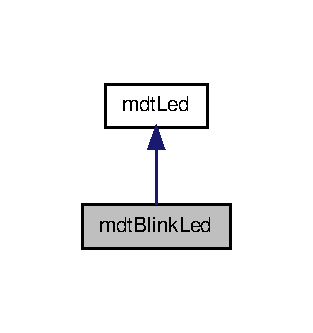
\includegraphics[width=150pt]{classmdt_blink_led__inherit__graph}
\end{center}
\end{figure}


Collaboration diagram for mdtBlinkLed:\nopagebreak
\begin{figure}[H]
\begin{center}
\leavevmode
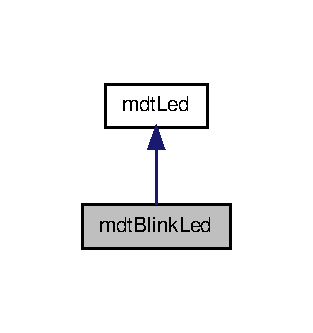
\includegraphics[width=150pt]{classmdt_blink_led__coll__graph}
\end{center}
\end{figure}
\subsection*{Public Slots}
\begin{DoxyCompactItemize}
\item 
void \hyperlink{classmdt_blink_led_ae51c54f31a11dbaebe69ab2c0b814d0f}{setOn} ()
\begin{DoxyCompactList}\small\item\em Set the LED ON. \end{DoxyCompactList}\item 
void \hyperlink{classmdt_blink_led_a951465e8a9ae5167e7eb05a7107ab13f}{setOff} ()
\begin{DoxyCompactList}\small\item\em Set the LED OFF. \end{DoxyCompactList}\end{DoxyCompactItemize}
\subsection*{Public Member Functions}
\begin{DoxyCompactItemize}
\item 
\hypertarget{classmdt_blink_led_abbc96bc408a45ceb191a908b2808a235}{
{\bfseries mdtBlinkLed} (QWidget $\ast$parent=0)}
\label{classmdt_blink_led_abbc96bc408a45ceb191a908b2808a235}

\item 
void \hyperlink{classmdt_blink_led_ae2dc395378aed0705ff19db5096a1efc}{setBlinkPeriod} (int T)
\begin{DoxyCompactList}\small\item\em Set blinking period. \end{DoxyCompactList}\item 
void \hyperlink{classmdt_blink_led_a1b15c8fafec0bc3aeb31ddf284ca7be2}{setBlinking} (bool on)
\begin{DoxyCompactList}\small\item\em Set LED blinking. \end{DoxyCompactList}\end{DoxyCompactItemize}


\subsection{Detailed Description}
Blinking LED. 

This class can be helpfull to get a blinking LED in a simple way.\par
 If a lot of blinking LED's are needed, it is recommanded to use \hyperlink{classmdt_led}{mdtLed} objects and one QTimer, and to connect the QTimer::timeout() signal to each \hyperlink{classmdt_led_a9e86ff65f2ec1bfb6131e2b9042609e8}{mdtLed::toggleOnOff()} slot. 

\subsection{Member Function Documentation}
\hypertarget{classmdt_blink_led_a1b15c8fafec0bc3aeb31ddf284ca7be2}{
\index{mdtBlinkLed@{mdtBlinkLed}!setBlinking@{setBlinking}}
\index{setBlinking@{setBlinking}!mdtBlinkLed@{mdtBlinkLed}}
\subsubsection[{setBlinking}]{\setlength{\rightskip}{0pt plus 5cm}void mdtBlinkLed::setBlinking (
\begin{DoxyParamCaption}
\item[{bool}]{on}
\end{DoxyParamCaption}
)}}
\label{classmdt_blink_led_a1b15c8fafec0bc3aeb31ddf284ca7be2}


Set LED blinking. 

Set the LED blinking. The blink period can be changed with \hyperlink{classmdt_blink_led_ae2dc395378aed0705ff19db5096a1efc}{setBlinkPeriod()} When \hyperlink{classmdt_blink_led_ae51c54f31a11dbaebe69ab2c0b814d0f}{setOn()} or \hyperlink{classmdt_blink_led_a951465e8a9ae5167e7eb05a7107ab13f}{setOff()} is called, the blinking is cancelled.


\begin{DoxyParams}{Parameters}
{\em on} & If true, the LED goes blinking. \\
\hline
\end{DoxyParams}
\hypertarget{classmdt_blink_led_ae2dc395378aed0705ff19db5096a1efc}{
\index{mdtBlinkLed@{mdtBlinkLed}!setBlinkPeriod@{setBlinkPeriod}}
\index{setBlinkPeriod@{setBlinkPeriod}!mdtBlinkLed@{mdtBlinkLed}}
\subsubsection[{setBlinkPeriod}]{\setlength{\rightskip}{0pt plus 5cm}void mdtBlinkLed::setBlinkPeriod (
\begin{DoxyParamCaption}
\item[{int}]{T}
\end{DoxyParamCaption}
)}}
\label{classmdt_blink_led_ae2dc395378aed0705ff19db5096a1efc}


Set blinking period. 

In 1 period, the LED toogles 1x ON ant 1x OFF (The time whenn the LED is ON is 1/2 period)


\begin{DoxyParams}{Parameters}
{\em T} & The period \mbox{[}ms\mbox{]} (min. 160 \mbox{[}ms\mbox{]}) \\
\hline
\end{DoxyParams}
\hypertarget{classmdt_blink_led_a951465e8a9ae5167e7eb05a7107ab13f}{
\index{mdtBlinkLed@{mdtBlinkLed}!setOff@{setOff}}
\index{setOff@{setOff}!mdtBlinkLed@{mdtBlinkLed}}
\subsubsection[{setOff}]{\setlength{\rightskip}{0pt plus 5cm}void mdtBlinkLed::setOff (
\begin{DoxyParamCaption}
{}
\end{DoxyParamCaption}
)\hspace{0.3cm}{\ttfamily  \mbox{[}slot\mbox{]}}}}
\label{classmdt_blink_led_a951465e8a9ae5167e7eb05a7107ab13f}


Set the LED OFF. 



Reimplemented from \hyperlink{classmdt_led_a4c8f5f6aa91b7c90ae6b1aa4933ba6e0}{mdtLed}.

\hypertarget{classmdt_blink_led_ae51c54f31a11dbaebe69ab2c0b814d0f}{
\index{mdtBlinkLed@{mdtBlinkLed}!setOn@{setOn}}
\index{setOn@{setOn}!mdtBlinkLed@{mdtBlinkLed}}
\subsubsection[{setOn}]{\setlength{\rightskip}{0pt plus 5cm}void mdtBlinkLed::setOn (
\begin{DoxyParamCaption}
{}
\end{DoxyParamCaption}
)\hspace{0.3cm}{\ttfamily  \mbox{[}slot\mbox{]}}}}
\label{classmdt_blink_led_ae51c54f31a11dbaebe69ab2c0b814d0f}


Set the LED ON. 



Reimplemented from \hyperlink{classmdt_led_a389ee3e0082ce8fa38cb258944a04892}{mdtLed}.



The documentation for this class was generated from the following files:\begin{DoxyCompactItemize}
\item 
src/mdtutilsgui/mdtBlinkLed.h\item 
src/mdtutilsgui/mdtBlinkLed.cpp\end{DoxyCompactItemize}

\hypertarget{classmdt_buffer}{\section{mdt\-Buffer$<$ T $>$ Class Template Reference}
\label{classmdt_buffer}\index{mdt\-Buffer$<$ T $>$@{mdt\-Buffer$<$ T $>$}}
}


Stockage d'éléments basé sur le principe du tampon circulaire.  




{\ttfamily \#include $<$mdt\-Buffer.\-h$>$}

\subsection*{Public Member Functions}
\begin{DoxyCompactItemize}
\item 
\hyperlink{classmdt_buffer_a51bc78e5a9fc926c7b898160c6a2faa3}{mdt\-Buffer} ()
\begin{DoxyCompactList}\small\item\em Constructeur. \end{DoxyCompactList}\item 
\hyperlink{classmdt_buffer_a4d6c140c02257fffb37016d019e412cf}{mdt\-Buffer} (\hyperlink{classmdt_buffer}{mdt\-Buffer}$<$ T $>$ \&src)
\begin{DoxyCompactList}\small\item\em Constructeur de copie. \end{DoxyCompactList}\item 
\hyperlink{classmdt_buffer}{mdt\-Buffer}$<$ T $>$ \& \hyperlink{classmdt_buffer_aba9a31eb29a39a2721205f13f80c1d8d}{operator=} (\hyperlink{classmdt_buffer}{mdt\-Buffer}$<$ T $>$ \&src)
\begin{DoxyCompactList}\small\item\em Opérateur de copie. \end{DoxyCompactList}\item 
\hyperlink{classmdt_buffer_a54de4cebee3cab7b8c1b86bfc3bdad4f}{$\sim$mdt\-Buffer} ()
\begin{DoxyCompactList}\small\item\em Destructeur. \end{DoxyCompactList}\item 
bool \hyperlink{classmdt_buffer_a9d081b06f666fec3ff6e12ec94b2a4fd}{init} (size\-\_\-t size)
\begin{DoxyCompactList}\small\item\em Initialisation du tampon. \end{DoxyCompactList}\item 
void \hyperlink{classmdt_buffer_a697920838a6c786209607c2b6ac0858a}{clear} ()
\begin{DoxyCompactList}\small\item\em Efface le contenu du tampon. \end{DoxyCompactList}\item 
size\-\_\-t \hyperlink{classmdt_buffer_abe03f0413ff7512d63d8df1408c66f63}{put} (const T $\ast$data, size\-\_\-t len)
\begin{DoxyCompactList}\small\item\em Stockage d'un lot de données. \end{DoxyCompactList}\item 
bool \hyperlink{classmdt_buffer_a2b9fd3a6b593c2e874249aba5c305e34}{put\-One} (T data)
\begin{DoxyCompactList}\small\item\em Stockage d'un élément par copie. \end{DoxyCompactList}\item 
size\-\_\-t \hyperlink{classmdt_buffer_a7beeb199f0cce529549e61ff949a9ffa}{put\-Until} (const T $\ast$data, T token, size\-\_\-t max\-Len, bool Ignore\-Null\-Values)
\begin{DoxyCompactList}\small\item\em Stockage d'un lot de données jusqu'à la rencontre d'un élément. \end{DoxyCompactList}\item 
bool \hyperlink{classmdt_buffer_a6ddc3c27c154fbfd077f83d5bfe82a19}{token\-Reached} ()
\begin{DoxyCompactList}\small\item\em Retourne true si l'élément de fin de copie à été atteint. \end{DoxyCompactList}\item 
size\-\_\-t \hyperlink{classmdt_buffer_aa6eddf7ccc533da855ebd112202a656f}{capacity} ()
\begin{DoxyCompactList}\small\item\em Capacité totale. \end{DoxyCompactList}\item 
size\-\_\-t \hyperlink{classmdt_buffer_a78e8317b6ba09e9c4e26358e27f75fd6}{remain\-Capacity} ()
\begin{DoxyCompactList}\small\item\em Capacité restante. \end{DoxyCompactList}\item 
bool \hyperlink{classmdt_buffer_a63e2b6b5e7656a5285d0ea1d152ea499}{full} ()
\begin{DoxyCompactList}\small\item\em Déterminer si le tampon est plein. \end{DoxyCompactList}\item 
size\-\_\-t \hyperlink{classmdt_buffer_a24ca1a2d00ba1623416ec747ba440adf}{available} ()
\begin{DoxyCompactList}\small\item\em Nombre d'éléments disponibles en lecture. \end{DoxyCompactList}\item 
size\-\_\-t \hyperlink{classmdt_buffer_a123a85c9cd59f80623aba5589709050e}{get} (T $\ast$data, size\-\_\-t len)
\begin{DoxyCompactList}\small\item\em Lecture d'un lot de données. \end{DoxyCompactList}\item 
size\-\_\-t \hyperlink{classmdt_buffer_a58e0f5bce9faea0f7c7195ff5377458c}{take} (T $\ast$data, size\-\_\-t len)
\begin{DoxyCompactList}\small\item\em Retrait d'un lot de données. \end{DoxyCompactList}\item 
T \hyperlink{classmdt_buffer_a690e3f41a62175de48bc73c19f69208d}{take\-One} ()
\begin{DoxyCompactList}\small\item\em Retrait d'un élément. \end{DoxyCompactList}\end{DoxyCompactItemize}


\subsection{Detailed Description}
\subsubsection*{template$<$class T$>$class mdt\-Buffer$<$ T $>$}

Stockage d'éléments basé sur le principe du tampon circulaire. 

\#if U\-S\-E\-\_\-\-A\-S\-S\-E\-R\-T == 1 \#undef N\-D\-E\-B\-U\-G \#else \#define N\-D\-E\-B\-U\-G \#endif

Stockage d'éléments basé sur le principe du tampon circulaire Idéal pour le stockage temporaire si une taille maximale est connue. Evite de nombreuses allocations/libération mémoire 

Definition at line 39 of file mdt\-Buffer.\-h.



\subsection{Constructor \& Destructor Documentation}
\hypertarget{classmdt_buffer_a51bc78e5a9fc926c7b898160c6a2faa3}{\index{mdt\-Buffer@{mdt\-Buffer}!mdt\-Buffer@{mdt\-Buffer}}
\index{mdt\-Buffer@{mdt\-Buffer}!mdtBuffer@{mdt\-Buffer}}
\subsubsection[{mdt\-Buffer}]{\setlength{\rightskip}{0pt plus 5cm}template$<$class T $>$ template {\bf mdt\-Buffer}$<$ T $>$\-::{\bf mdt\-Buffer} (
\begin{DoxyParamCaption}
{}
\end{DoxyParamCaption}
)}}\label{classmdt_buffer_a51bc78e5a9fc926c7b898160c6a2faa3}


Constructeur. 

Constructeur, utiliser \hyperlink{classmdt_buffer_a9d081b06f666fec3ff6e12ec94b2a4fd}{init()} avant tout autre opération 

Definition at line 7 of file mdt\-Buffer.\-cpp.

\hypertarget{classmdt_buffer_a4d6c140c02257fffb37016d019e412cf}{\index{mdt\-Buffer@{mdt\-Buffer}!mdt\-Buffer@{mdt\-Buffer}}
\index{mdt\-Buffer@{mdt\-Buffer}!mdtBuffer@{mdt\-Buffer}}
\subsubsection[{mdt\-Buffer}]{\setlength{\rightskip}{0pt plus 5cm}template$<$class T $>$ {\bf mdt\-Buffer}$<$ T $>$\-::{\bf mdt\-Buffer} (
\begin{DoxyParamCaption}
\item[{{\bf mdt\-Buffer}$<$ T $>$ \&}]{src}
\end{DoxyParamCaption}
)}}\label{classmdt_buffer_a4d6c140c02257fffb37016d019e412cf}


Constructeur de copie. 

Constructeur de copie. Effectue une copie des données vers l'autre instance 

Definition at line 16 of file mdt\-Buffer.\-cpp.



References mdt\-Buffer$<$ T $>$\-::available(), mdt\-Buffer$<$ T $>$\-::capacity(), and mdt\-Buffer$<$ T $>$\-::get().

\hypertarget{classmdt_buffer_a54de4cebee3cab7b8c1b86bfc3bdad4f}{\index{mdt\-Buffer@{mdt\-Buffer}!$\sim$mdt\-Buffer@{$\sim$mdt\-Buffer}}
\index{$\sim$mdt\-Buffer@{$\sim$mdt\-Buffer}!mdtBuffer@{mdt\-Buffer}}
\subsubsection[{$\sim$mdt\-Buffer}]{\setlength{\rightskip}{0pt plus 5cm}template$<$class T $>$ template {\bf mdt\-Buffer}$<$ T $>$\-::$\sim${\bf mdt\-Buffer} (
\begin{DoxyParamCaption}
{}
\end{DoxyParamCaption}
)}}\label{classmdt_buffer_a54de4cebee3cab7b8c1b86bfc3bdad4f}


Destructeur. 

Destructeur 

Definition at line 59 of file mdt\-Buffer.\-cpp.



\subsection{Member Function Documentation}
\hypertarget{classmdt_buffer_a24ca1a2d00ba1623416ec747ba440adf}{\index{mdt\-Buffer@{mdt\-Buffer}!available@{available}}
\index{available@{available}!mdtBuffer@{mdt\-Buffer}}
\subsubsection[{available}]{\setlength{\rightskip}{0pt plus 5cm}template$<$class T $>$ template size\-\_\-t {\bf mdt\-Buffer}$<$ T $>$\-::available (
\begin{DoxyParamCaption}
{}
\end{DoxyParamCaption}
)}}\label{classmdt_buffer_a24ca1a2d00ba1623416ec747ba440adf}


Nombre d'éléments disponibles en lecture. 

Nombre d'éléments disponibles en lecture

\begin{DoxyReturn}{Returns}
Le nombre d'éléments qu'il est possible de lire 
\end{DoxyReturn}


Definition at line 236 of file mdt\-Buffer.\-cpp.



Referenced by mdt\-Buffer$<$ T $>$\-::mdt\-Buffer(), and mdt\-Buffer$<$ T $>$\-::operator=().

\hypertarget{classmdt_buffer_aa6eddf7ccc533da855ebd112202a656f}{\index{mdt\-Buffer@{mdt\-Buffer}!capacity@{capacity}}
\index{capacity@{capacity}!mdtBuffer@{mdt\-Buffer}}
\subsubsection[{capacity}]{\setlength{\rightskip}{0pt plus 5cm}template$<$class T $>$ template size\-\_\-t {\bf mdt\-Buffer}$<$ T $>$\-::capacity (
\begin{DoxyParamCaption}
{}
\end{DoxyParamCaption}
)}}\label{classmdt_buffer_aa6eddf7ccc533da855ebd112202a656f}


Capacité totale. 

Capacité totale

\begin{DoxyReturn}{Returns}
La capacité totale du tampon 
\end{DoxyReturn}


Definition at line 221 of file mdt\-Buffer.\-cpp.



Referenced by mdt\-Buffer$<$ T $>$\-::mdt\-Buffer(), and mdt\-Buffer$<$ T $>$\-::operator=().

\hypertarget{classmdt_buffer_a697920838a6c786209607c2b6ac0858a}{\index{mdt\-Buffer@{mdt\-Buffer}!clear@{clear}}
\index{clear@{clear}!mdtBuffer@{mdt\-Buffer}}
\subsubsection[{clear}]{\setlength{\rightskip}{0pt plus 5cm}template$<$class T $>$ template void {\bf mdt\-Buffer}$<$ T $>$\-::clear (
\begin{DoxyParamCaption}
{}
\end{DoxyParamCaption}
)}}\label{classmdt_buffer_a697920838a6c786209607c2b6ac0858a}


Efface le contenu du tampon. 

Efface le contenu du tampon. La quantité disponible ainsi que la capacité restante sont aussi ré-\/initialisés 

Definition at line 88 of file mdt\-Buffer.\-cpp.

\hypertarget{classmdt_buffer_a63e2b6b5e7656a5285d0ea1d152ea499}{\index{mdt\-Buffer@{mdt\-Buffer}!full@{full}}
\index{full@{full}!mdtBuffer@{mdt\-Buffer}}
\subsubsection[{full}]{\setlength{\rightskip}{0pt plus 5cm}template$<$class T $>$ template bool {\bf mdt\-Buffer}$<$ T $>$\-::full (
\begin{DoxyParamCaption}
{}
\end{DoxyParamCaption}
)}}\label{classmdt_buffer_a63e2b6b5e7656a5285d0ea1d152ea499}


Déterminer si le tampon est plein. 

Déterminer si le tampon est plein

\begin{DoxyReturn}{Returns}
True si le tampon est plein 
\end{DoxyReturn}


Definition at line 231 of file mdt\-Buffer.\-cpp.

\hypertarget{classmdt_buffer_a123a85c9cd59f80623aba5589709050e}{\index{mdt\-Buffer@{mdt\-Buffer}!get@{get}}
\index{get@{get}!mdtBuffer@{mdt\-Buffer}}
\subsubsection[{get}]{\setlength{\rightskip}{0pt plus 5cm}template$<$class T $>$ template size\-\_\-t {\bf mdt\-Buffer}$<$ T $>$\-::get (
\begin{DoxyParamCaption}
\item[{T $\ast$}]{data, }
\item[{size\-\_\-t}]{len}
\end{DoxyParamCaption}
)}}\label{classmdt_buffer_a123a85c9cd59f80623aba5589709050e}


Lecture d'un lot de données. 

La copie, basée sur memcpy, est performante Le cusreur de lecture interne, ainsi que le quantité disponible et la capacité restante ne sont pas altérés (plusieurs appels à cette méthode renverrait chaque fois les même données)


\begin{DoxyParams}{Parameters}
{\em data} & Pointeur vers les données de destination \\
\hline
{\em len} & Nombre d'éléments à lire\\
\hline
\end{DoxyParams}
\begin{DoxyReturn}{Returns}
Le nombre d'éléments effectivement lus 
\end{DoxyReturn}


Definition at line 241 of file mdt\-Buffer.\-cpp.



Referenced by mdt\-Buffer$<$ T $>$\-::mdt\-Buffer(), and mdt\-Buffer$<$ T $>$\-::operator=().

\hypertarget{classmdt_buffer_a9d081b06f666fec3ff6e12ec94b2a4fd}{\index{mdt\-Buffer@{mdt\-Buffer}!init@{init}}
\index{init@{init}!mdtBuffer@{mdt\-Buffer}}
\subsubsection[{init}]{\setlength{\rightskip}{0pt plus 5cm}template$<$class T $>$ template bool {\bf mdt\-Buffer}$<$ T $>$\-::init (
\begin{DoxyParamCaption}
\item[{size\-\_\-t}]{size}
\end{DoxyParamCaption}
)}}\label{classmdt_buffer_a9d081b06f666fec3ff6e12ec94b2a4fd}


Initialisation du tampon. 

Initialisation du tampon. Alloue la mémoire, initialise les données à une valeur nulle. Il est possible de ré-\/appeler cette fonction plusieurs fois, la zone mémoire étant alors ré-\/alouée


\begin{DoxyParams}{Parameters}
{\em size} & Capacité du tampon \mbox{[}nombre d'éléments\mbox{]}\\
\hline
\end{DoxyParams}
\begin{DoxyReturn}{Returns}
false en cas de problème d'allocation mémoire (true si tout s'est bien passé) 
\end{DoxyReturn}


Definition at line 66 of file mdt\-Buffer.\-cpp.

\hypertarget{classmdt_buffer_aba9a31eb29a39a2721205f13f80c1d8d}{\index{mdt\-Buffer@{mdt\-Buffer}!operator=@{operator=}}
\index{operator=@{operator=}!mdtBuffer@{mdt\-Buffer}}
\subsubsection[{operator=}]{\setlength{\rightskip}{0pt plus 5cm}template$<$class T $>$ template {\bf mdt\-Buffer}$<$ char $>$ \& {\bf mdt\-Buffer}$<$ T $>$\-::operator= (
\begin{DoxyParamCaption}
\item[{{\bf mdt\-Buffer}$<$ T $>$ \&}]{src}
\end{DoxyParamCaption}
)}}\label{classmdt_buffer_aba9a31eb29a39a2721205f13f80c1d8d}


Opérateur de copie. 

Opérateur de copie. Effectue une copie des données vers l'autre instance 

Definition at line 38 of file mdt\-Buffer.\-cpp.



References mdt\-Buffer$<$ T $>$\-::available(), mdt\-Buffer$<$ T $>$\-::capacity(), and mdt\-Buffer$<$ T $>$\-::get().

\hypertarget{classmdt_buffer_abe03f0413ff7512d63d8df1408c66f63}{\index{mdt\-Buffer@{mdt\-Buffer}!put@{put}}
\index{put@{put}!mdtBuffer@{mdt\-Buffer}}
\subsubsection[{put}]{\setlength{\rightskip}{0pt plus 5cm}template$<$class T $>$ template size\-\_\-t {\bf mdt\-Buffer}$<$ T $>$\-::put (
\begin{DoxyParamCaption}
\item[{const T $\ast$}]{data, }
\item[{size\-\_\-t}]{len}
\end{DoxyParamCaption}
)}}\label{classmdt_buffer_abe03f0413ff7512d63d8df1408c66f63}


Stockage d'un lot de données. 

Stockage d'un lot de données par copie. La copie, basée sur memcpy, est performante


\begin{DoxyParams}{Parameters}
{\em data} & Pointeur vers les données sources \\
\hline
{\em len} & Nombre d'éléments à stocker\\
\hline
\end{DoxyParams}
\begin{DoxyReturn}{Returns}
Le nombre d'éléments effectivement stockés 
\end{DoxyReturn}


Definition at line 107 of file mdt\-Buffer.\-cpp.

\hypertarget{classmdt_buffer_a2b9fd3a6b593c2e874249aba5c305e34}{\index{mdt\-Buffer@{mdt\-Buffer}!put\-One@{put\-One}}
\index{put\-One@{put\-One}!mdtBuffer@{mdt\-Buffer}}
\subsubsection[{put\-One}]{\setlength{\rightskip}{0pt plus 5cm}template$<$class T $>$ template bool {\bf mdt\-Buffer}$<$ T $>$\-::put\-One (
\begin{DoxyParamCaption}
\item[{T}]{data}
\end{DoxyParamCaption}
)}}\label{classmdt_buffer_a2b9fd3a6b593c2e874249aba5c305e34}


Stockage d'un élément par copie. 

Stockage d'un élément par copie.


\begin{DoxyParams}{Parameters}
{\em data} & Elément à stocker\\
\hline
\end{DoxyParams}
\begin{DoxyReturn}{Returns}
True si Ok, false en cas d'erreur 
\end{DoxyReturn}


Definition at line 155 of file mdt\-Buffer.\-cpp.



References inc\-Wr\-Cursor.

\hypertarget{classmdt_buffer_a7beeb199f0cce529549e61ff949a9ffa}{\index{mdt\-Buffer@{mdt\-Buffer}!put\-Until@{put\-Until}}
\index{put\-Until@{put\-Until}!mdtBuffer@{mdt\-Buffer}}
\subsubsection[{put\-Until}]{\setlength{\rightskip}{0pt plus 5cm}template$<$class T $>$ template size\-\_\-t {\bf mdt\-Buffer}$<$ T $>$\-::put\-Until (
\begin{DoxyParamCaption}
\item[{const T $\ast$}]{data, }
\item[{T}]{token, }
\item[{size\-\_\-t}]{max\-Len, }
\item[{bool}]{Ignore\-Null\-Values}
\end{DoxyParamCaption}
)}}\label{classmdt_buffer_a7beeb199f0cce529549e61ff949a9ffa}


Stockage d'un lot de données jusqu'à la rencontre d'un élément. 

Stockage d'un lot de données par copie jusqu'à la rencontre d'un élément, ou max\-Len si l'élément recherché n'est pas trouvé. L'élément de recherche est aussi stocké La copie, basée sur une boucle, est relativement lente (comparé à memcpy) Il est possible de ne pas stocker les caractères null ('\textbackslash{}0')


\begin{DoxyParams}{Parameters}
{\em data} & Pointeur vers les données sources \\
\hline
{\em token} & Elément désignant la fin de la copie \\
\hline
{\em Maxlen} & Nombre d'éléments maximal à stocker \\
\hline
{\em Ignore\-Null\-Values} & Si true, les éléments null (0) ne seront pas stockés\\
\hline
\end{DoxyParams}
\begin{DoxyReturn}{Returns}
Le nombre d'éléments effectivement stockés 
\end{DoxyReturn}


Definition at line 175 of file mdt\-Buffer.\-cpp.



References inc\-Wr\-Cursor.

\hypertarget{classmdt_buffer_a78e8317b6ba09e9c4e26358e27f75fd6}{\index{mdt\-Buffer@{mdt\-Buffer}!remain\-Capacity@{remain\-Capacity}}
\index{remain\-Capacity@{remain\-Capacity}!mdtBuffer@{mdt\-Buffer}}
\subsubsection[{remain\-Capacity}]{\setlength{\rightskip}{0pt plus 5cm}template$<$class T $>$ template size\-\_\-t {\bf mdt\-Buffer}$<$ T $>$\-::remain\-Capacity (
\begin{DoxyParamCaption}
{}
\end{DoxyParamCaption}
)}}\label{classmdt_buffer_a78e8317b6ba09e9c4e26358e27f75fd6}


Capacité restante. 

Capacité restante

\begin{DoxyReturn}{Returns}
Le nombre d'éléments qu'il est encore possible de stocker 
\end{DoxyReturn}


Definition at line 226 of file mdt\-Buffer.\-cpp.

\hypertarget{classmdt_buffer_a58e0f5bce9faea0f7c7195ff5377458c}{\index{mdt\-Buffer@{mdt\-Buffer}!take@{take}}
\index{take@{take}!mdtBuffer@{mdt\-Buffer}}
\subsubsection[{take}]{\setlength{\rightskip}{0pt plus 5cm}template$<$class T $>$ template size\-\_\-t {\bf mdt\-Buffer}$<$ T $>$\-::take (
\begin{DoxyParamCaption}
\item[{T $\ast$}]{data, }
\item[{size\-\_\-t}]{len}
\end{DoxyParamCaption}
)}}\label{classmdt_buffer_a58e0f5bce9faea0f7c7195ff5377458c}


Retrait d'un lot de données. 

Retrait d'un lot de données par copie. La copie, basée sur memcpy, et performante Le cusreur de lecture interne, ainsi que le quantité disponible et la capacité restante sont altérés


\begin{DoxyParams}{Parameters}
{\em data} & Pointeur vers les données de destination \\
\hline
{\em len} & Nombre d'éléments à lire\\
\hline
\end{DoxyParams}
\begin{DoxyReturn}{Returns}
Le nombre d'éléments effectivement retirés 
\end{DoxyReturn}


Definition at line 280 of file mdt\-Buffer.\-cpp.

\hypertarget{classmdt_buffer_a690e3f41a62175de48bc73c19f69208d}{\index{mdt\-Buffer@{mdt\-Buffer}!take\-One@{take\-One}}
\index{take\-One@{take\-One}!mdtBuffer@{mdt\-Buffer}}
\subsubsection[{take\-One}]{\setlength{\rightskip}{0pt plus 5cm}template$<$class T $>$ template std\-::string {\bf mdt\-Buffer}$<$ T $>$\-::take\-One (
\begin{DoxyParamCaption}
{}
\end{DoxyParamCaption}
)}}\label{classmdt_buffer_a690e3f41a62175de48bc73c19f69208d}


Retrait d'un élément. 

Retrait d'un élément Le cusreur de lecture interne, ainsi que le quantité disponible et la capacité restante sont altérés Test retour\-: 0 est retourné si aucun élément n'est disponible. Etant donnée que 0 peut très bien être un élément valide stocké dans le tampon, il faut utiliser une méthode de test avant le retrait. Voir \hyperlink{classmdt_buffer_a24ca1a2d00ba1623416ec747ba440adf}{available()}

\begin{DoxyReturn}{Returns}
Un élément, ou 0 si aucune disponibilité 
\end{DoxyReturn}


Definition at line 326 of file mdt\-Buffer.\-cpp.



References inc\-Rd\-Cursor.

\hypertarget{classmdt_buffer_a6ddc3c27c154fbfd077f83d5bfe82a19}{\index{mdt\-Buffer@{mdt\-Buffer}!token\-Reached@{token\-Reached}}
\index{token\-Reached@{token\-Reached}!mdtBuffer@{mdt\-Buffer}}
\subsubsection[{token\-Reached}]{\setlength{\rightskip}{0pt plus 5cm}template$<$class T $>$ template bool {\bf mdt\-Buffer}$<$ T $>$\-::token\-Reached (
\begin{DoxyParamCaption}
{}
\end{DoxyParamCaption}
)}}\label{classmdt_buffer_a6ddc3c27c154fbfd077f83d5bfe82a19}


Retourne true si l'élément de fin de copie à été atteint. 

Retourne true si l'élément de fin de copie à été atteint Voir la méthode \hyperlink{classmdt_buffer_a7beeb199f0cce529549e61ff949a9ffa}{put\-Until()} Ce flag est effacé par un appel de la méthode \hyperlink{classmdt_buffer_a58e0f5bce9faea0f7c7195ff5377458c}{take()} , même si l'élément n'est pas \char`\"{}consommé\char`\"{} \hyperlink{classmdt_buffer_a697920838a6c786209607c2b6ac0858a}{clear()} efface aussi ce flag

\begin{DoxyReturn}{Returns}
True si l'élément de fin à été atteint 
\end{DoxyReturn}


Definition at line 216 of file mdt\-Buffer.\-cpp.



The documentation for this class was generated from the following files\-:\begin{DoxyCompactItemize}
\item 
src/mdtutils/\hyperlink{mdt_buffer_8h}{mdt\-Buffer.\-h}\item 
src/mdtutils/\hyperlink{mdt_buffer_8cpp}{mdt\-Buffer.\-cpp}\end{DoxyCompactItemize}

\hypertarget{classmdt_csv_file}{
\section{mdtCsvFile Class Reference}
\label{classmdt_csv_file}\index{mdtCsvFile@{mdtCsvFile}}
}


Read and write CSV file.  




{\ttfamily \#include $<$mdtCsvFile.h$>$}

\subsection*{Public Member Functions}
\begin{DoxyCompactItemize}
\item 
\hypertarget{classmdt_csv_file_a8c9f24190d83f32672f360f0fcc53d2f}{
\hyperlink{classmdt_csv_file_a8c9f24190d83f32672f360f0fcc53d2f}{mdtCsvFile} (QObject $\ast$parent=0, QByteArray fileEncoding=\char`\"{}UTF-\/8\char`\"{})}
\label{classmdt_csv_file_a8c9f24190d83f32672f360f0fcc53d2f}

\begin{DoxyCompactList}\small\item\em Constructor. \end{DoxyCompactList}\item 
bool \hyperlink{classmdt_csv_file_ab2d9754e50db179825813081bb129797}{readLines} (QByteArray separator=\char`\"{};\char`\"{}, QByteArray dataProtection=\char`\"{}\char`\"{}, QByteArray comment=\char`\"{}\#\char`\"{})
\begin{DoxyCompactList}\small\item\em Read the file and store data. \end{DoxyCompactList}\item 
QStringList \& \hyperlink{classmdt_csv_file_af44de864675351a6f22b176e64a4cecc}{parseLine} (const QByteArray \&line, const QByteArray \&separator, const QByteArray \&dataProtection)
\begin{DoxyCompactList}\small\item\em Parse a string (considered as a line in a CSV file) \end{DoxyCompactList}\item 
\hypertarget{classmdt_csv_file_afe815d4fbdc08c442c9b1dce447cda75}{
void \hyperlink{classmdt_csv_file_afe815d4fbdc08c442c9b1dce447cda75}{clear} ()}
\label{classmdt_csv_file_afe815d4fbdc08c442c9b1dce447cda75}

\begin{DoxyCompactList}\small\item\em Clear readen data. \end{DoxyCompactList}\item 
QString \hyperlink{classmdt_csv_file_af2d0917f92dd0d0d8100edccf1d3e4ee}{valueAt} (int line, int column)
\begin{DoxyCompactList}\small\item\em Get a value. \end{DoxyCompactList}\item 
\hypertarget{classmdt_csv_file_a089e82f55982a40587f3d9e53c7ff261}{
QList$<$ QStringList $>$ \& \hyperlink{classmdt_csv_file_a089e82f55982a40587f3d9e53c7ff261}{lines} ()}
\label{classmdt_csv_file_a089e82f55982a40587f3d9e53c7ff261}

\begin{DoxyCompactList}\small\item\em Get content of entire file. \end{DoxyCompactList}\end{DoxyCompactItemize}


\subsection{Detailed Description}
Read and write CSV file. 

The default file encoding format is assumed UTF-\/8. If another format is to use, give it at constructor. 

Definition at line 35 of file mdtCsvFile.h.



\subsection{Member Function Documentation}
\hypertarget{classmdt_csv_file_af44de864675351a6f22b176e64a4cecc}{
\index{mdtCsvFile@{mdtCsvFile}!parseLine@{parseLine}}
\index{parseLine@{parseLine}!mdtCsvFile@{mdtCsvFile}}
\subsubsection[{parseLine}]{\setlength{\rightskip}{0pt plus 5cm}QStringList \& mdtCsvFile::parseLine (
\begin{DoxyParamCaption}
\item[{const QByteArray \&}]{line, }
\item[{const QByteArray \&}]{separator, }
\item[{const QByteArray \&}]{dataProtection}
\end{DoxyParamCaption}
)}}
\label{classmdt_csv_file_af44de864675351a6f22b176e64a4cecc}


Parse a string (considered as a line in a CSV file) 


\begin{DoxyParams}{Parameters}
{\em separator} & Separator to use (typical: ; ) \\
\hline
{\em protection} & Data protection (typical: " ) \\
\hline
\end{DoxyParams}
\begin{DoxyReturn}{Returns}
The list of found fields 
\end{DoxyReturn}


Definition at line 71 of file mdtCsvFile.cpp.

\hypertarget{classmdt_csv_file_ab2d9754e50db179825813081bb129797}{
\index{mdtCsvFile@{mdtCsvFile}!readLines@{readLines}}
\index{readLines@{readLines}!mdtCsvFile@{mdtCsvFile}}
\subsubsection[{readLines}]{\setlength{\rightskip}{0pt plus 5cm}bool mdtCsvFile::readLines (
\begin{DoxyParamCaption}
\item[{QByteArray}]{separator = {\ttfamily \char`\"{};\char`\"{}}, }
\item[{QByteArray}]{dataProtection = {\ttfamily \char`\"{}\char`\"{}}, }
\item[{QByteArray}]{comment = {\ttfamily \char`\"{}\#\char`\"{}}}
\end{DoxyParamCaption}
)}}
\label{classmdt_csv_file_ab2d9754e50db179825813081bb129797}


Read the file and store data. 


\begin{DoxyParams}{Parameters}
{\em separator} & Separator to use (typical: ; ) \\
\hline
{\em protection} & Data protection (typical: " ) \\
\hline
{\em comment} & Comment (typical: \# ) \\
\hline
\end{DoxyParams}
\begin{DoxyReturn}{Returns}
True on success, false else (see errorString() to know what happened in this case) 
\end{DoxyReturn}
\begin{DoxyPrecond}{Precondition}
separator, dataProtection and comment must not be the same 
\end{DoxyPrecond}


Definition at line 37 of file mdtCsvFile.cpp.

\hypertarget{classmdt_csv_file_af2d0917f92dd0d0d8100edccf1d3e4ee}{
\index{mdtCsvFile@{mdtCsvFile}!valueAt@{valueAt}}
\index{valueAt@{valueAt}!mdtCsvFile@{mdtCsvFile}}
\subsubsection[{valueAt}]{\setlength{\rightskip}{0pt plus 5cm}QString mdtCsvFile::valueAt (
\begin{DoxyParamCaption}
\item[{int}]{line, }
\item[{int}]{column}
\end{DoxyParamCaption}
)}}
\label{classmdt_csv_file_af2d0917f92dd0d0d8100edccf1d3e4ee}


Get a value. 

No value is available before \hyperlink{classmdt_csv_file_ab2d9754e50db179825813081bb129797}{readLines()} was called. If requested index (line, column) is empty, or does not exists, a empty string is returned. The index check is done internally. 

Definition at line 160 of file mdtCsvFile.cpp.



The documentation for this class was generated from the following files:\begin{DoxyCompactItemize}
\item 
src/mdtutils/mdtCsvFile.h\item 
src/mdtutils/mdtCsvFile.cpp\end{DoxyCompactItemize}

\hypertarget{classmdt_data_widget_mapper}{
\section{mdtDataWidgetMapper Class Reference}
\label{classmdt_data_widget_mapper}\index{mdtDataWidgetMapper@{mdtDataWidgetMapper}}
}


DataWidget mapper.  




{\ttfamily \#include $<$mdtDataWidgetMapper.h$>$}



Collaboration diagram for mdtDataWidgetMapper:
\nopagebreak
\begin{figure}[H]
\begin{center}
\leavevmode
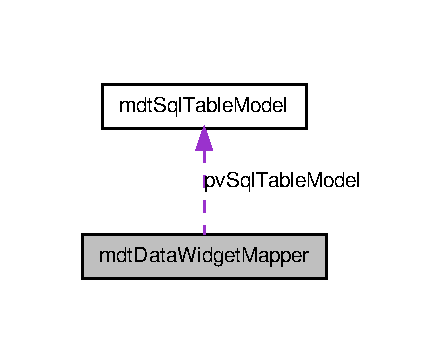
\includegraphics[width=214pt]{classmdt_data_widget_mapper__coll__graph}
\end{center}
\end{figure}
\subsection*{Public Member Functions}
\begin{DoxyCompactItemize}
\item 
\hypertarget{classmdt_data_widget_mapper_a0569659cfdde7a3be8626d0c0e1f785e}{
{\bfseries mdtDataWidgetMapper} (QObject $\ast$parent=0)}
\label{classmdt_data_widget_mapper_a0569659cfdde7a3be8626d0c0e1f785e}

\item 
void \hyperlink{classmdt_data_widget_mapper_af2f866ef24395911b1aca49a7ce7ca3e}{setModel} (\hyperlink{classmdt_sql_table_model}{mdtSqlTableModel} $\ast$model)
\begin{DoxyCompactList}\small\item\em Set the model. \end{DoxyCompactList}\item 
\hypertarget{classmdt_data_widget_mapper_ab01a124254cf4b2795b800c8c4df04d0}{
\hyperlink{classmdt_sql_table_model}{mdtSqlTableModel} $\ast$ \hyperlink{classmdt_data_widget_mapper_ab01a124254cf4b2795b800c8c4df04d0}{model} ()}
\label{classmdt_data_widget_mapper_ab01a124254cf4b2795b800c8c4df04d0}

\begin{DoxyCompactList}\small\item\em Get the model instance. \end{DoxyCompactList}\item 
void \hyperlink{classmdt_data_widget_mapper_a02a1109d55f5c553667a7fb9c02e70c1}{addMapping} (QWidget $\ast$widget, int section)
\begin{DoxyCompactList}\small\item\em Adds a mapping between a widget and a section from the model. \end{DoxyCompactList}\item 
void \hyperlink{classmdt_data_widget_mapper_a9bb91385d70c7017db79507af0ed8960}{addMapping} (QWidget $\ast$widget, int section, const QByteArray \&propertyName)
\begin{DoxyCompactList}\small\item\em Adds a mapping between a widget and a section from the model. \end{DoxyCompactList}\end{DoxyCompactItemize}


\subsection{Detailed Description}
DataWidget mapper. 

\subsection{Member Function Documentation}
\hypertarget{classmdt_data_widget_mapper_a02a1109d55f5c553667a7fb9c02e70c1}{
\index{mdtDataWidgetMapper@{mdtDataWidgetMapper}!addMapping@{addMapping}}
\index{addMapping@{addMapping}!mdtDataWidgetMapper@{mdtDataWidgetMapper}}
\subsubsection[{addMapping}]{\setlength{\rightskip}{0pt plus 5cm}void mdtDataWidgetMapper::addMapping (
\begin{DoxyParamCaption}
\item[{QWidget $\ast$}]{widget, }
\item[{int}]{section}
\end{DoxyParamCaption}
)}}
\label{classmdt_data_widget_mapper_a02a1109d55f5c553667a7fb9c02e70c1}


Adds a mapping between a widget and a section from the model. 

This method uses the widget name (objectName), and tries to find the field (in database) that has the same name.\par
 If field is found, some attributes are set (f.ex: read only, mandatory field, ...). At last step, QDataWidgetMapper::addMapping() is called. \begin{DoxyPrecond}{Precondition}
A valid model must be set with \hyperlink{classmdt_data_widget_mapper_af2f866ef24395911b1aca49a7ce7ca3e}{setModel()} 

widget must be a valid pointer 
\end{DoxyPrecond}
\hypertarget{classmdt_data_widget_mapper_a9bb91385d70c7017db79507af0ed8960}{
\index{mdtDataWidgetMapper@{mdtDataWidgetMapper}!addMapping@{addMapping}}
\index{addMapping@{addMapping}!mdtDataWidgetMapper@{mdtDataWidgetMapper}}
\subsubsection[{addMapping}]{\setlength{\rightskip}{0pt plus 5cm}void mdtDataWidgetMapper::addMapping (
\begin{DoxyParamCaption}
\item[{QWidget $\ast$}]{widget, }
\item[{int}]{section, }
\item[{const QByteArray \&}]{propertyName}
\end{DoxyParamCaption}
)}}
\label{classmdt_data_widget_mapper_a9bb91385d70c7017db79507af0ed8960}


Adds a mapping between a widget and a section from the model. 

\begin{DoxySeeAlso}{See also}
\hyperlink{classmdt_data_widget_mapper_a02a1109d55f5c553667a7fb9c02e70c1}{addMapping()} 
\end{DoxySeeAlso}
\hypertarget{classmdt_data_widget_mapper_af2f866ef24395911b1aca49a7ce7ca3e}{
\index{mdtDataWidgetMapper@{mdtDataWidgetMapper}!setModel@{setModel}}
\index{setModel@{setModel}!mdtDataWidgetMapper@{mdtDataWidgetMapper}}
\subsubsection[{setModel}]{\setlength{\rightskip}{0pt plus 5cm}void mdtDataWidgetMapper::setModel (
\begin{DoxyParamCaption}
\item[{{\bf mdtSqlTableModel} $\ast$}]{model}
\end{DoxyParamCaption}
)}}
\label{classmdt_data_widget_mapper_af2f866ef24395911b1aca49a7ce7ca3e}


Set the model. 

Note that a \hyperlink{classmdt_sql_table_model}{mdtSqlTableModel} instance is requierd, because database fields attributes are used internally. \begin{DoxyPrecond}{Precondition}
model must be a pointer to a valid instance. 
\end{DoxyPrecond}


The documentation for this class was generated from the following files:\begin{DoxyCompactItemize}
\item 
src/mdtutilsgui/mdtDataWidgetMapper.h\item 
src/mdtutilsgui/mdtDataWidgetMapper.cpp\end{DoxyCompactItemize}

\hypertarget{classmdt_device}{
\section{mdtDevice Class Reference}
\label{classmdt_device}\index{mdtDevice@{mdtDevice}}
}


Base class for a device connected to a port.  




{\ttfamily \#include $<$mdtDevice.h$>$}



Inheritance diagram for mdtDevice:\nopagebreak
\begin{figure}[H]
\begin{center}
\leavevmode
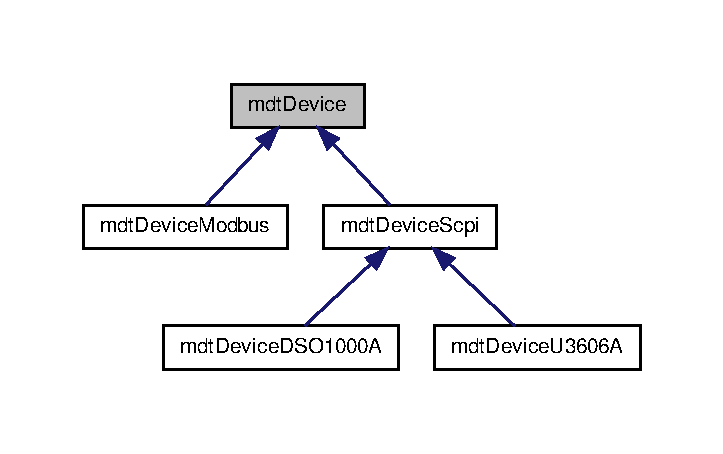
\includegraphics[width=400pt]{classmdt_device__inherit__graph}
\end{center}
\end{figure}


Collaboration diagram for mdtDevice:\nopagebreak
\begin{figure}[H]
\begin{center}
\leavevmode
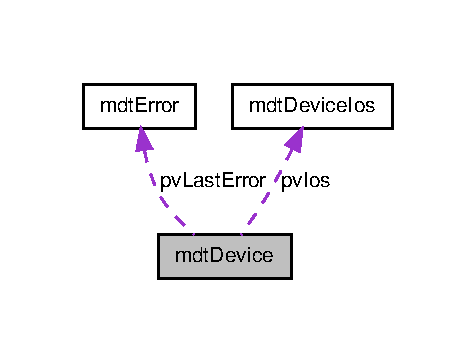
\includegraphics[width=156pt]{classmdt_device__coll__graph}
\end{center}
\end{figure}
\subsection*{Public Slots}
\begin{DoxyCompactItemize}
\item 
void \hyperlink{classmdt_device_a83cdf442f4cec7261742ca5939e390a1}{setAnalogOutputValue} (\hyperlink{classmdt_analog_io}{mdtAnalogIo} $\ast$analogOutput)
\begin{DoxyCompactList}\small\item\em Set value on a analog output on physical device. \end{DoxyCompactList}\item 
void \hyperlink{classmdt_device_a93abbc706a1e6601ce947eee5e50fba6}{setDigitalOutputValue} (\hyperlink{classmdt_digital_io}{mdtDigitalIo} $\ast$digitalOutput)
\begin{DoxyCompactList}\small\item\em Set value on a digital output on physical device. \end{DoxyCompactList}\item 
void \hyperlink{classmdt_device_a14634fec6cd6bae810562b3bd88a5c05}{runQueries} ()
\begin{DoxyCompactList}\small\item\em Queries to send periodically. \end{DoxyCompactList}\end{DoxyCompactItemize}
\subsection*{Signals}
\begin{DoxyCompactItemize}
\item 
void \hyperlink{classmdt_device_aecd2d9d2cc3665f2084d0fd20eb3db2d}{stateChanged} (int state)
\begin{DoxyCompactList}\small\item\em Emitted when state has changed. \end{DoxyCompactList}\item 
void \hyperlink{classmdt_device_a3fbc6e71241e2e9daa2d8557f870c03c}{statusMessageChanged} (const QString \&message, const QString \&details, int timeout)
\begin{DoxyCompactList}\small\item\em Emitted when a new status message is to display. \end{DoxyCompactList}\end{DoxyCompactItemize}
\subsection*{Public Member Functions}
\begin{DoxyCompactItemize}
\item 
\hyperlink{classmdt_device_a6d501791e7243358cc61b144254b80db}{mdtDevice} (QObject $\ast$parent=0)
\begin{DoxyCompactList}\small\item\em Construct a device object. \end{DoxyCompactList}\item 
virtual \hyperlink{classmdt_device_ac2a9cfd6042f3f9d8da4e84f044d3f4a}{$\sim$mdtDevice} ()
\begin{DoxyCompactList}\small\item\em Destructor. \end{DoxyCompactList}\item 
\hypertarget{classmdt_device_a80186f1aa6fbdc13f1652de978c35518}{
void \hyperlink{classmdt_device_a80186f1aa6fbdc13f1652de978c35518}{setName} (const QString \&name)}
\label{classmdt_device_a80186f1aa6fbdc13f1652de978c35518}

\begin{DoxyCompactList}\small\item\em Set the device name. \end{DoxyCompactList}\item 
\hypertarget{classmdt_device_a7ad893c6885dbaef5a6cb980bfe627e0}{
QString \hyperlink{classmdt_device_a7ad893c6885dbaef5a6cb980bfe627e0}{name} () const }
\label{classmdt_device_a7ad893c6885dbaef5a6cb980bfe627e0}

\begin{DoxyCompactList}\small\item\em Get device name. \end{DoxyCompactList}\item 
virtual \hyperlink{classmdt_abstract_port_ad4121bb930c95887e77f8bafa065a85e}{mdtAbstractPort::error\_\-t} \hyperlink{classmdt_device_abab1b6e45af527880ce469ae318474c0}{connectToDevice} (const \hyperlink{classmdt_device_info}{mdtDeviceInfo} \&devInfo)
\begin{DoxyCompactList}\small\item\em Search and connect to physical device. \end{DoxyCompactList}\item 
void \hyperlink{classmdt_device_a9f1de62ef54974b0636dee673bd819e2}{setIos} (\hyperlink{classmdt_device_ios}{mdtDeviceIos} $\ast$ios, bool autoOutputUpdate=false)
\begin{DoxyCompactList}\small\item\em Set the I/O's container. \end{DoxyCompactList}\item 
void \hyperlink{classmdt_device_aa241c40514683254990e742cf1bbb155}{setBackToReadyStateTimeout} (int timeout)
\begin{DoxyCompactList}\small\item\em Set back to ready state timeout. \end{DoxyCompactList}\item 
virtual \hyperlink{classmdt_port_manager}{mdtPortManager} $\ast$ \hyperlink{classmdt_device_a06d9178b4133fd7b23084e712af20976}{portManager} ()
\begin{DoxyCompactList}\small\item\em Get internal port manager instance. \end{DoxyCompactList}\item 
void \hyperlink{classmdt_device_a721c5bf2cfa0eef5304333f08da182f7}{start} (int queryInterval)
\begin{DoxyCompactList}\small\item\em Start periodic device querying. \end{DoxyCompactList}\item 
\hypertarget{classmdt_device_adc7ff8f01d68506283a3d0cc6bc25407}{
void \hyperlink{classmdt_device_adc7ff8f01d68506283a3d0cc6bc25407}{stop} ()}
\label{classmdt_device_adc7ff8f01d68506283a3d0cc6bc25407}

\begin{DoxyCompactList}\small\item\em Stop periodic device querying. \end{DoxyCompactList}\item 
\hyperlink{classmdt_value}{mdtValue} \hyperlink{classmdt_device_ab828764660ba53ffce1995901ddf5a0a}{getAnalogInputValue} (\hyperlink{classmdt_analog_io}{mdtAnalogIo} $\ast$analogInput, bool queryDevice, bool waitOnReply)
\begin{DoxyCompactList}\small\item\em Get analog input value. \end{DoxyCompactList}\item 
\hypertarget{classmdt_device_ad6a9d73cd51ce21f69dc8e4646d4fcfe}{
\hyperlink{classmdt_value}{mdtValue} {\bfseries getAnalogInputValue} (int address, bool queryDevice, bool waitOnReply)}
\label{classmdt_device_ad6a9d73cd51ce21f69dc8e4646d4fcfe}

\item 
\hypertarget{classmdt_device_a66a4c466dd6cb5c8235850f6dc23ae7b}{
\hyperlink{classmdt_value}{mdtValue} {\bfseries getAnalogInputValue} (const QString \&labelShort, bool queryDevice, bool waitOnReply)}
\label{classmdt_device_a66a4c466dd6cb5c8235850f6dc23ae7b}

\item 
int \hyperlink{classmdt_device_a98cba3132db15317daf54eb701388e91}{getAnalogInputs} (bool waitOnReply)
\begin{DoxyCompactList}\small\item\em Read all analog inputs on physical device and update (G)UI representation. \end{DoxyCompactList}\item 
\hyperlink{classmdt_value}{mdtValue} \hyperlink{classmdt_device_a163ee286d905feafe50b3e4351d4bf41}{getAnalogOutputValue} (\hyperlink{classmdt_analog_io}{mdtAnalogIo} $\ast$analogOutput, bool queryDevice, bool waitOnReply)
\begin{DoxyCompactList}\small\item\em Get analog output value. \end{DoxyCompactList}\item 
\hypertarget{classmdt_device_aa90eb1111d6778f4227224d3b1804ae7}{
\hyperlink{classmdt_value}{mdtValue} {\bfseries getAnalogOutputValue} (int addressRead, bool queryDevice, bool waitOnReply)}
\label{classmdt_device_aa90eb1111d6778f4227224d3b1804ae7}

\item 
\hypertarget{classmdt_device_ad6bfbab4c93bc0136068e773dd776010}{
\hyperlink{classmdt_value}{mdtValue} {\bfseries getAnalogOutputValue} (const QString \&labelShort, bool queryDevice, bool waitOnReply)}
\label{classmdt_device_ad6bfbab4c93bc0136068e773dd776010}

\item 
int \hyperlink{classmdt_device_a78a8968cf61c1cac518b0a8af471110c}{getAnalogOutputs} (bool waitOnReply)
\begin{DoxyCompactList}\small\item\em Read all analog outputs on physical device and update (G)UI representation. \end{DoxyCompactList}\item 
int \hyperlink{classmdt_device_a766d9adcf8c2274f61f120a4a5c5c6d9}{setAnalogOutputValue} (\hyperlink{classmdt_analog_io}{mdtAnalogIo} $\ast$analogOutput, const \hyperlink{classmdt_value}{mdtValue} \&value, bool sendToDevice, bool waitOnReply)
\begin{DoxyCompactList}\small\item\em Set analog output value. \end{DoxyCompactList}\item 
\hypertarget{classmdt_device_ab605f81f28271f54570f151e94039807}{
int {\bfseries setAnalogOutputValue} (int addressWrite, const \hyperlink{classmdt_value}{mdtValue} \&value, bool sendToDevice, bool waitOnReply)}
\label{classmdt_device_ab605f81f28271f54570f151e94039807}

\item 
\hypertarget{classmdt_device_a40b49f882622c37f50a57132f954e732}{
int {\bfseries setAnalogOutputValue} (const QString \&labelShort, const \hyperlink{classmdt_value}{mdtValue} \&value, bool sendToDevice, bool waitOnReply)}
\label{classmdt_device_a40b49f882622c37f50a57132f954e732}

\item 
int \hyperlink{classmdt_device_a57e1cee7e670469035c57e3bd2ff4c9d}{setAnalogOutputs} (bool waitOnReply)
\begin{DoxyCompactList}\small\item\em Write all analog outputs on physical device and update (G)UI representation. \end{DoxyCompactList}\item 
\hyperlink{classmdt_value}{mdtValue} \hyperlink{classmdt_device_afe8bd7811ccc4a2ba8088edf073e0a8d}{getDigitalInputValue} (\hyperlink{classmdt_digital_io}{mdtDigitalIo} $\ast$digitalInput, bool queryDevice, bool waitOnReply)
\begin{DoxyCompactList}\small\item\em Get digital input value. \end{DoxyCompactList}\item 
\hypertarget{classmdt_device_a9915b677a307ffeab98a413d61b0f2e7}{
\hyperlink{classmdt_value}{mdtValue} {\bfseries getDigitalInputValue} (int address, bool queryDevice, bool waitOnReply)}
\label{classmdt_device_a9915b677a307ffeab98a413d61b0f2e7}

\item 
\hypertarget{classmdt_device_a295a2795695804cc291282d92a1c7641}{
\hyperlink{classmdt_value}{mdtValue} {\bfseries getDigitalInputValue} (const QString \&labelShort, bool queryDevice, bool waitOnReply)}
\label{classmdt_device_a295a2795695804cc291282d92a1c7641}

\item 
int \hyperlink{classmdt_device_a6e338b959c86591b6b3401f925c49050}{getDigitalInputs} (bool waitOnReply)
\begin{DoxyCompactList}\small\item\em Read all digital inputs on physical device and update (G)UI representation. \end{DoxyCompactList}\item 
\hyperlink{classmdt_value}{mdtValue} \hyperlink{classmdt_device_a978bde9f2b6177b6f3742163e7a712a9}{getDigitalOutputValue} (\hyperlink{classmdt_digital_io}{mdtDigitalIo} $\ast$digitalOutput, bool queryDevice, bool waitOnReply)
\begin{DoxyCompactList}\small\item\em Get digital output value. \end{DoxyCompactList}\item 
\hypertarget{classmdt_device_adf8160df55a9eb9ba6820e24bb7f1440}{
\hyperlink{classmdt_value}{mdtValue} {\bfseries getDigitalOutputValue} (int addressRead, bool queryDevice, bool waitOnReply)}
\label{classmdt_device_adf8160df55a9eb9ba6820e24bb7f1440}

\item 
\hypertarget{classmdt_device_a5e7b7de4243f45d8cfa42599d51555bf}{
\hyperlink{classmdt_value}{mdtValue} {\bfseries getDigitalOutputValue} (const QString \&labelShort, bool queryDevice, bool waitOnReply)}
\label{classmdt_device_a5e7b7de4243f45d8cfa42599d51555bf}

\item 
int \hyperlink{classmdt_device_ab35b81b8eb68e161ac06ae882be39a25}{getDigitalOutputs} (bool waitOnReply)
\begin{DoxyCompactList}\small\item\em Read all digital outputs on physical device and update (G)UI representation. \end{DoxyCompactList}\item 
int \hyperlink{classmdt_device_a04564fd9be440c026e7c399f0e619485}{setDigitalOutputValue} (\hyperlink{classmdt_digital_io}{mdtDigitalIo} $\ast$digitalOutput, const \hyperlink{classmdt_value}{mdtValue} \&value, bool sendToDevice, bool waitOnReply)
\begin{DoxyCompactList}\small\item\em Set a digital output value. \end{DoxyCompactList}\item 
\hypertarget{classmdt_device_a5c2514c3c31a687a01a898c874d2c45e}{
int {\bfseries setDigitalOutputValue} (int addressWrite, const \hyperlink{classmdt_value}{mdtValue} \&value, bool sendToDevice, bool waitOnReply)}
\label{classmdt_device_a5c2514c3c31a687a01a898c874d2c45e}

\item 
\hypertarget{classmdt_device_a2377d24cc1e767a24dfc5e34454a8737}{
int {\bfseries setDigitalOutputValue} (const QString \&labelShort, const \hyperlink{classmdt_value}{mdtValue} \&value, bool sendToDevice, bool waitOnReply)}
\label{classmdt_device_a2377d24cc1e767a24dfc5e34454a8737}

\item 
int \hyperlink{classmdt_device_a7b86a816e55a91f0d62426e1741437c6}{setDigitalOutputs} (bool waitOnReply)
\begin{DoxyCompactList}\small\item\em Write all digital outputs to physical device and update (G)UI representation. \end{DoxyCompactList}\item 
\hypertarget{classmdt_device_a76ddf08ac78502b835b192a8f38f963f}{
\hyperlink{classmdt_port_manager_a9448339d7f08ca5e18b904df25b382da}{mdtPortManager::state\_\-t} \hyperlink{classmdt_device_a76ddf08ac78502b835b192a8f38f963f}{currentState} ()}
\label{classmdt_device_a76ddf08ac78502b835b192a8f38f963f}

\begin{DoxyCompactList}\small\item\em Get device state. \end{DoxyCompactList}\end{DoxyCompactItemize}
\subsection*{Protected Slots}
\begin{DoxyCompactItemize}
\item 
virtual void \hyperlink{classmdt_device_ad211ba3be781c3db0397d5bf91f796d1}{decodeReadenFrame} (\hyperlink{classmdt_port_transaction}{mdtPortTransaction} $\ast$transaction)
\begin{DoxyCompactList}\small\item\em Decode incoming frames. \end{DoxyCompactList}\end{DoxyCompactItemize}
\subsection*{Protected Member Functions}
\begin{DoxyCompactItemize}
\item 
virtual int \hyperlink{classmdt_device_acecf7934ce29b3a957accb0f4c98c746}{readAnalogInput} (\hyperlink{classmdt_port_transaction}{mdtPortTransaction} $\ast$transaction)
\begin{DoxyCompactList}\small\item\em Read one analog input on physical device. \end{DoxyCompactList}\item 
virtual int \hyperlink{classmdt_device_a40674e7bf0c367bb3edb407d73a5bd8e}{readAnalogInputs} (\hyperlink{classmdt_port_transaction}{mdtPortTransaction} $\ast$transaction)
\begin{DoxyCompactList}\small\item\em Read all analog inputs on physical device. \end{DoxyCompactList}\item 
virtual int \hyperlink{classmdt_device_a7934063c3f41a742515f1232c9598c2a}{readAnalogOutput} (\hyperlink{classmdt_port_transaction}{mdtPortTransaction} $\ast$transaction)
\begin{DoxyCompactList}\small\item\em Read one analog output on physical device. \end{DoxyCompactList}\item 
virtual int \hyperlink{classmdt_device_ab0232ac83c38bc93d3bc2aa91d94c291}{readAnalogOutputs} (\hyperlink{classmdt_port_transaction}{mdtPortTransaction} $\ast$transaction)
\begin{DoxyCompactList}\small\item\em Read all analog outputs on physical device. \end{DoxyCompactList}\item 
virtual int \hyperlink{classmdt_device_ae764634bba2b321ac2b4731c0353e45f}{writeAnalogOutput} (int value, \hyperlink{classmdt_port_transaction}{mdtPortTransaction} $\ast$transaction)
\begin{DoxyCompactList}\small\item\em Write value on a analog output to physical device. \end{DoxyCompactList}\item 
virtual int \hyperlink{classmdt_device_abc52b797df29945bf0a6358aab1b7245}{writeAnalogOutputs} (\hyperlink{classmdt_port_transaction}{mdtPortTransaction} $\ast$transaction)
\begin{DoxyCompactList}\small\item\em Write all analog outputs to physical device. \end{DoxyCompactList}\item 
virtual int \hyperlink{classmdt_device_af128b606050035abaf8d049bb2227015}{readDigitalInput} (\hyperlink{classmdt_port_transaction}{mdtPortTransaction} $\ast$transaction)
\begin{DoxyCompactList}\small\item\em Read one digital input on physical device. \end{DoxyCompactList}\item 
virtual int \hyperlink{classmdt_device_a150e3abae6db5bf1ad11017bf2b76c14}{readDigitalInputs} (\hyperlink{classmdt_port_transaction}{mdtPortTransaction} $\ast$transaction)
\begin{DoxyCompactList}\small\item\em Read all digital inputs on physical device. \end{DoxyCompactList}\item 
virtual int \hyperlink{classmdt_device_a1faee6ab31b094731211ea0943544501}{readDigitalOutput} (\hyperlink{classmdt_port_transaction}{mdtPortTransaction} $\ast$transaction)
\begin{DoxyCompactList}\small\item\em Read one digital output on physical device. \end{DoxyCompactList}\item 
virtual int \hyperlink{classmdt_device_aac038c24c3b91757584bdf0d09fb8b02}{readDigitalOutputs} (\hyperlink{classmdt_port_transaction}{mdtPortTransaction} $\ast$transaction)
\begin{DoxyCompactList}\small\item\em Read all digital outputs on physical device. \end{DoxyCompactList}\item 
virtual int \hyperlink{classmdt_device_a0fbe57503d86554829e708b2b83d73f1}{writeDigitalOutput} (bool state, \hyperlink{classmdt_port_transaction}{mdtPortTransaction} $\ast$transaction)
\begin{DoxyCompactList}\small\item\em Write state on a digital output to physical device. \end{DoxyCompactList}\item 
virtual int \hyperlink{classmdt_device_aa9e8ae7b4ff2455b4105d280d8523fc1}{writeDigitalOutputs} (\hyperlink{classmdt_port_transaction}{mdtPortTransaction} $\ast$transaction)
\begin{DoxyCompactList}\small\item\em Write all digital outputs to physical device. \end{DoxyCompactList}\item 
virtual bool \hyperlink{classmdt_device_acba50968d201ad95c4eaa2ab2ed48b4f}{queriesSequence} ()
\begin{DoxyCompactList}\small\item\em Sequence of queries to send periodically. \end{DoxyCompactList}\item 
\hyperlink{classmdt_port_transaction}{mdtPortTransaction} $\ast$ \hyperlink{classmdt_device_a0e57cc8b749581cff447d514b9a1ff8e}{getNewTransaction} ()
\begin{DoxyCompactList}\small\item\em Get a new transaction. \end{DoxyCompactList}\item 
void \hyperlink{classmdt_device_a4619d8be240cafe48865a89f7424de92}{restoreTransaction} (\hyperlink{classmdt_port_transaction}{mdtPortTransaction} $\ast$transaction)
\begin{DoxyCompactList}\small\item\em Restore a transaction into pool. \end{DoxyCompactList}\item 
bool \hyperlink{classmdt_device_ab937015c1a319b7234442a4cc29a02a8}{waitTransactionDone} (int id)
\begin{DoxyCompactList}\small\item\em Wait until a transaction is done without break the GUI's event loop. \end{DoxyCompactList}\end{DoxyCompactItemize}
\subsection*{Protected Attributes}
\begin{DoxyCompactItemize}
\item 
\hypertarget{classmdt_device_aa84e01b13f98fc35476a2654f1c8d2b3}{
\hyperlink{classmdt_device_ios}{mdtDeviceIos} $\ast$ {\bfseries pvIos}}
\label{classmdt_device_aa84e01b13f98fc35476a2654f1c8d2b3}

\end{DoxyCompactItemize}


\subsection{Detailed Description}
Base class for a device connected to a port. 

Querying a device can be done several ways. Some devices sends a confirmation after each query.

Some queries (f.ex. read a input value or state) give a result after query. In some applications, we need to display the reult priodically. In other application, we need to send the query and wait on result before we can continue. This base class gives a interface for these two cases.

At basis, all query methods are not blocking by default. The normal way is to connect \hyperlink{classmdt_port_manager_a416a24db1048e9f66aef27ea810954d2}{mdtPortManager::newTransactionDone()} to \hyperlink{classmdt_device_ad211ba3be781c3db0397d5bf91f796d1}{decodeReadenFrame()} slot (must be done in subclass). This way, a query will be sent to device and method returns. When device returns a result, \hyperlink{classmdt_port_manager}{mdtPortManager} will send the newTransactionDone() signal, and decoding will be processed in \hyperlink{classmdt_device_ad211ba3be781c3db0397d5bf91f796d1}{decodeReadenFrame()} and I/O's are updated.

Because the blocking behaviour is sometimes needed, the concept of transaction was implemented in \hyperlink{classmdt_port_manager}{mdtPortManager}. At first, we tell the query method (for example \hyperlink{classmdt_device_ab828764660ba53ffce1995901ddf5a0a}{getAnalogInputValue()} ) that we will wait on a reply by setting the waitOnReply flag. Then, the query is sent to device and a transaction ID is added to a list (see \hyperlink{classmdt_port_manager}{mdtPortManager} for details). At next, \hyperlink{classmdt_device_ab937015c1a319b7234442a4cc29a02a8}{waitTransactionDone()} is called, and finally result is returned. Note that \hyperlink{classmdt_device_ab937015c1a319b7234442a4cc29a02a8}{waitTransactionDone()} will not breack the Qt's event loop because it uses the mdtPortManager::wait() method (see documentation of \hyperlink{classmdt_port_manager}{mdtPortManager} for details).

If it is needed to continiusly update the representation of device's inputs (digital/analog I/O, voltage, temperature, ...), two things can happen:
\begin{DoxyItemize}
\item 1) Used port can receive data continiusly (f.ex. RS232) and device send data automatically
\item 2) Used port need that a request is sent for each read (TCP, USB, ...) or device need such request Continous update is typical usefull for a GUI representing a real device.
\end{DoxyItemize}

A other usage is automated sequence. In this case, the sequence will tell when it need to set a output and when a input value is reuqierd.

A device can accept one or many request before results must be read. This depends most case on used port and protocol.

It can be useful to find on witch port a device is attached (f.ex. setup of a automated test application). For this, \hyperlink{classmdt_device_abab1b6e45af527880ce469ae318474c0}{connectToDevice()} was introduced.

A device can have several states (ready, busy, disconnected, ...). To help the application programmer to keep consistency, this states are updated in this class using \hyperlink{classmdt_port_manager}{mdtPortManager} 's state machine. This state machine is based on QStateMachine. 

Definition at line 89 of file mdtDevice.h.



\subsection{Constructor \& Destructor Documentation}
\hypertarget{classmdt_device_a6d501791e7243358cc61b144254b80db}{
\index{mdtDevice@{mdtDevice}!mdtDevice@{mdtDevice}}
\index{mdtDevice@{mdtDevice}!mdtDevice@{mdtDevice}}
\subsubsection[{mdtDevice}]{\setlength{\rightskip}{0pt plus 5cm}mdtDevice::mdtDevice (
\begin{DoxyParamCaption}
\item[{QObject $\ast$}]{parent = {\ttfamily 0}}
\end{DoxyParamCaption}
)}}
\label{classmdt_device_a6d501791e7243358cc61b144254b80db}


Construct a device object. 



\hyperlink{classmdt_device_a76ddf08ac78502b835b192a8f38f963f}{currentState()} = \hyperlink{classmdt_port_manager_a9448339d7f08ca5e18b904df25b382daa4004253e25d51b1e628bb5006dbbd153}{mdtPortManager::Disconnected}; setStateDisconnected(); connect(pvBackToReadyStateTimer, SIGNAL(timeout()), this, SLOT(setStateReady())); connect(pvBackToReadyStateTimer, SIGNAL(timeout()), this, SIGNAL(deviceReady())); 



Definition at line 30 of file mdtDevice.cpp.

\hypertarget{classmdt_device_ac2a9cfd6042f3f9d8da4e84f044d3f4a}{
\index{mdtDevice@{mdtDevice}!$\sim$mdtDevice@{$\sim$mdtDevice}}
\index{$\sim$mdtDevice@{$\sim$mdtDevice}!mdtDevice@{mdtDevice}}
\subsubsection[{$\sim$mdtDevice}]{\setlength{\rightskip}{0pt plus 5cm}mdtDevice::$\sim$mdtDevice (
\begin{DoxyParamCaption}
{}
\end{DoxyParamCaption}
)\hspace{0.3cm}{\ttfamily  \mbox{[}virtual\mbox{]}}}}
\label{classmdt_device_ac2a9cfd6042f3f9d8da4e84f044d3f4a}


Destructor. 

If queries sequence is running, it will be stopped (see \hyperlink{classmdt_device_adc7ff8f01d68506283a3d0cc6bc25407}{stop()} ). 

Definition at line 49 of file mdtDevice.cpp.



\subsection{Member Function Documentation}
\hypertarget{classmdt_device_abab1b6e45af527880ce469ae318474c0}{
\index{mdtDevice@{mdtDevice}!connectToDevice@{connectToDevice}}
\index{connectToDevice@{connectToDevice}!mdtDevice@{mdtDevice}}
\subsubsection[{connectToDevice}]{\setlength{\rightskip}{0pt plus 5cm}{\bf mdtAbstractPort::error\_\-t} mdtDevice::connectToDevice (
\begin{DoxyParamCaption}
\item[{const {\bf mdtDeviceInfo} \&}]{devInfo}
\end{DoxyParamCaption}
)\hspace{0.3cm}{\ttfamily  \mbox{[}virtual\mbox{]}}}}
\label{classmdt_device_abab1b6e45af527880ce469ae318474c0}


Search and connect to physical device. 

Will scan available ports and open the first port that has device attached matching request.


\begin{DoxyParams}{Parameters}
{\em devInfo} & Requested device's informations. \\
\hline
\end{DoxyParams}
\begin{DoxyReturn}{Returns}
A error listed in \hyperlink{classmdt_abstract_port_ad4121bb930c95887e77f8bafa065a85e}{mdtAbstractPort::error\_\-t} (NoError on success)
\end{DoxyReturn}
Note: default implementation does nothing and returns allways a UnhandledError. See subclass documentation for more details. 

Reimplemented in \hyperlink{classmdt_device_d_s_o1000_a_a84431cf929750a8a25d5218893736c72}{mdtDeviceDSO1000A}, \hyperlink{classmdt_device_modbus_wago_a025f0411a708a529054a0e3c0b6461cd}{mdtDeviceModbusWago}, \hyperlink{classmdt_device_scpi_ae8e886b362cbf9d1bf7064b48348b8e8}{mdtDeviceScpi}, and \hyperlink{classmdt_device_u3606_a_acf3b48b13bc179ad4f94b3011b7d607a}{mdtDeviceU3606A}.



Definition at line 65 of file mdtDevice.cpp.

\hypertarget{classmdt_device_ad211ba3be781c3db0397d5bf91f796d1}{
\index{mdtDevice@{mdtDevice}!decodeReadenFrame@{decodeReadenFrame}}
\index{decodeReadenFrame@{decodeReadenFrame}!mdtDevice@{mdtDevice}}
\subsubsection[{decodeReadenFrame}]{\setlength{\rightskip}{0pt plus 5cm}void mdtDevice::decodeReadenFrame (
\begin{DoxyParamCaption}
\item[{{\bf mdtPortTransaction} $\ast$}]{transaction}
\end{DoxyParamCaption}
)\hspace{0.3cm}{\ttfamily  \mbox{[}protected, virtual, slot\mbox{]}}}}
\label{classmdt_device_ad211ba3be781c3db0397d5bf91f796d1}


Decode incoming frames. 

Subclass notes:
\begin{DoxyItemize}
\item This default implementation does nothing.
\item This slot should be connected with \hyperlink{classmdt_port_manager_a416a24db1048e9f66aef27ea810954d2}{mdtPortManager::newTransactionDone(mdtPortTransaction$\ast$)} signal.
\item In this class, this connection is not made, it is the sublcass responsability to do this.
\item Once decoding was done, the concerned I/O(s) sould be updated with new value, or set to invalid value on error (see \hyperlink{classmdt_value}{mdtValue} class). Doing so will keep (G)UI consistency. 
\end{DoxyItemize}

Definition at line 898 of file mdtDevice.cpp.

\hypertarget{classmdt_device_a98cba3132db15317daf54eb701388e91}{
\index{mdtDevice@{mdtDevice}!getAnalogInputs@{getAnalogInputs}}
\index{getAnalogInputs@{getAnalogInputs}!mdtDevice@{mdtDevice}}
\subsubsection[{getAnalogInputs}]{\setlength{\rightskip}{0pt plus 5cm}int mdtDevice::getAnalogInputs (
\begin{DoxyParamCaption}
\item[{bool}]{waitOnReply}
\end{DoxyParamCaption}
)}}
\label{classmdt_device_a98cba3132db15317daf54eb701388e91}


Read all analog inputs on physical device and update (G)UI representation. 

Will call \hyperlink{classmdt_device_a40674e7bf0c367bb3edb407d73a5bd8e}{readAnalogInputs()}, witch also sends the request to device. Depending on result, device's state can be updated.

Behaviour of this method can vary, depending on device specific subclass. (See sublcass \hyperlink{classmdt_device_a40674e7bf0c367bb3edb407d73a5bd8e}{readAnalogInputs()} for details).

Once results are available or error occured, the internal analog inputs are updated. (See \hyperlink{classmdt_device_ios}{mdtDeviceIos} for details).


\begin{DoxyParams}{Parameters}
{\em waitOnReply} & If true, this method will wait until reply comes in, or timeout (See \hyperlink{classmdt_device_ab937015c1a319b7234442a4cc29a02a8}{waitTransactionDone()} ), else it will return immediately after the query was sent. \\
\hline
\end{DoxyParams}
\begin{DoxyReturn}{Returns}
0 or a ID on success. If no I/O's are set, on timeout or other error, a value $<$ 0 is returned. 
\end{DoxyReturn}


Definition at line 215 of file mdtDevice.cpp.

\hypertarget{classmdt_device_ab828764660ba53ffce1995901ddf5a0a}{
\index{mdtDevice@{mdtDevice}!getAnalogInputValue@{getAnalogInputValue}}
\index{getAnalogInputValue@{getAnalogInputValue}!mdtDevice@{mdtDevice}}
\subsubsection[{getAnalogInputValue}]{\setlength{\rightskip}{0pt plus 5cm}mdtDevice::getAnalogInputValue (
\begin{DoxyParamCaption}
\item[{{\bf mdtAnalogIo} $\ast$}]{analogInput, }
\item[{bool}]{queryDevice, }
\item[{bool}]{waitOnReply}
\end{DoxyParamCaption}
)}}
\label{classmdt_device_ab828764660ba53ffce1995901ddf5a0a}


Get analog input value. 

Get device or internal analog value. Internal value is updated if queryDevice is set.


\begin{DoxyParams}{Parameters}
{\em analogInput} & Pointer to a analog input object. \\
\hline
{\em queryDevice} & If true, value is readen from device by calling \hyperlink{classmdt_device_acecf7934ce29b3a957accb0f4c98c746}{readAnalogInput()}, else cached value is returned. Behaviour of this method can vary, depending on device specific subclass. (See sublcass \hyperlink{classmdt_device_acecf7934ce29b3a957accb0f4c98c746}{readAnalogInput()} for details). \\
\hline
{\em waitOnReply} & If true, this method will wait until reply comes in, or timeout (See \hyperlink{classmdt_device_ab937015c1a319b7234442a4cc29a02a8}{waitTransactionDone()} ), else it will return immediately after the query was sent. \\
\hline
\end{DoxyParams}
\begin{DoxyReturn}{Returns}
A \hyperlink{classmdt_value}{mdtValue} with valueDouble as real value and valueInt as device specific encoded fromat (if available). See \hyperlink{classmdt_value}{mdtValue} documentation for details about validity and other flags. 
\end{DoxyReturn}
\begin{DoxyPrecond}{Precondition}
analogInput must be valid.
\end{DoxyPrecond}
This is an overloaded member function, provided for convenience. It differs from the above function only in what argument(s) it accepts.


\begin{DoxyParams}{Parameters}
{\em address} & Depending on device organisation and protocol, this can be a relative or absolute address (f.ex. MODBUS queries), a input number, etc...\\
\hline
\end{DoxyParams}
This is an overloaded member function, provided for convenience. It differs from the above function only in what argument(s) it accepts.


\begin{DoxyParams}{Parameters}
{\em labelShort} & Short label set in I/O (see \hyperlink{classmdt_analog_io}{mdtAnalogIo} for details). \\
\hline
\end{DoxyParams}


Definition at line 134 of file mdtDevice.cpp.

\hypertarget{classmdt_device_a78a8968cf61c1cac518b0a8af471110c}{
\index{mdtDevice@{mdtDevice}!getAnalogOutputs@{getAnalogOutputs}}
\index{getAnalogOutputs@{getAnalogOutputs}!mdtDevice@{mdtDevice}}
\subsubsection[{getAnalogOutputs}]{\setlength{\rightskip}{0pt plus 5cm}int mdtDevice::getAnalogOutputs (
\begin{DoxyParamCaption}
\item[{bool}]{waitOnReply}
\end{DoxyParamCaption}
)}}
\label{classmdt_device_a78a8968cf61c1cac518b0a8af471110c}


Read all analog outputs on physical device and update (G)UI representation. 

Will call \hyperlink{classmdt_device_ab0232ac83c38bc93d3bc2aa91d94c291}{readAnalogOutputs()}, witch also sends the request to device. Depending on result, device's state can be updated.

Behaviour of this method can vary, depending on device specific subclass. (See sublcass \hyperlink{classmdt_device_ab0232ac83c38bc93d3bc2aa91d94c291}{readAnalogOutputs()} for details).

Once results are available or error occured, the internal analog outputs are updated. (See \hyperlink{classmdt_device_ios}{mdtDeviceIos} for details).


\begin{DoxyParams}{Parameters}
{\em waitOnReply} & If true, this method will wait until reply comes in, or timeout (See \hyperlink{classmdt_device_ab937015c1a319b7234442a4cc29a02a8}{waitTransactionDone()} ), else it will return immediately after the query was sent. \\
\hline
\end{DoxyParams}
\begin{DoxyReturn}{Returns}
0 or a ID on success. If no I/O's are set, on timeout or other error, a value $<$ 0 is returned. 
\end{DoxyReturn}


Definition at line 335 of file mdtDevice.cpp.

\hypertarget{classmdt_device_a163ee286d905feafe50b3e4351d4bf41}{
\index{mdtDevice@{mdtDevice}!getAnalogOutputValue@{getAnalogOutputValue}}
\index{getAnalogOutputValue@{getAnalogOutputValue}!mdtDevice@{mdtDevice}}
\subsubsection[{getAnalogOutputValue}]{\setlength{\rightskip}{0pt plus 5cm}mdtDevice::getAnalogOutputValue (
\begin{DoxyParamCaption}
\item[{{\bf mdtAnalogIo} $\ast$}]{analogOutput, }
\item[{bool}]{queryDevice, }
\item[{bool}]{waitOnReply}
\end{DoxyParamCaption}
)}}
\label{classmdt_device_a163ee286d905feafe50b3e4351d4bf41}


Get analog output value. 

Get device or internal analog value. Internal value is updated if queryDevice is set.


\begin{DoxyParams}{Parameters}
{\em analogOutput} & Pointer to a analog output object. \\
\hline
{\em queryDevice} & If true, value is readen from device by calling \hyperlink{classmdt_device_a7934063c3f41a742515f1232c9598c2a}{readAnalogOutput()}, else cached value is returned. Behaviour of this method can vary, depending on device specific subclass. (See sublcass \hyperlink{classmdt_device_a7934063c3f41a742515f1232c9598c2a}{readAnalogOutput()} for details). \\
\hline
{\em waitOnReply} & If true, this method will wait until reply comes in, or timeout (See \hyperlink{classmdt_device_ab937015c1a319b7234442a4cc29a02a8}{waitTransactionDone()} ), else it will return immediately after the query was sent. \\
\hline
\end{DoxyParams}
\begin{DoxyReturn}{Returns}
A \hyperlink{classmdt_value}{mdtValue} with valueDouble as real value and valueInt as device specific encoded fromat (if available). See \hyperlink{classmdt_value}{mdtValue} documentation for details about validity and other flags. 
\end{DoxyReturn}
\begin{DoxyPrecond}{Precondition}
analogOutput must be valid.
\end{DoxyPrecond}
This is an overloaded member function, provided for convenience. It differs from the above function only in what argument(s) it accepts.


\begin{DoxyParams}{Parameters}
{\em addressRead} & Depending on device organisation and protocol, this can be a relative or absolute address (f.ex. MODBUS queries), a output number, etc...\\
\hline
\end{DoxyParams}
This is an overloaded member function, provided for convenience. It differs from the above function only in what argument(s) it accepts.


\begin{DoxyParams}{Parameters}
{\em labelShort} & Short label set in I/O (see \hyperlink{classmdt_analog_io}{mdtAnalogIo} for details). \\
\hline
\end{DoxyParams}


Definition at line 255 of file mdtDevice.cpp.

\hypertarget{classmdt_device_a6e338b959c86591b6b3401f925c49050}{
\index{mdtDevice@{mdtDevice}!getDigitalInputs@{getDigitalInputs}}
\index{getDigitalInputs@{getDigitalInputs}!mdtDevice@{mdtDevice}}
\subsubsection[{getDigitalInputs}]{\setlength{\rightskip}{0pt plus 5cm}int mdtDevice::getDigitalInputs (
\begin{DoxyParamCaption}
\item[{bool}]{waitOnReply}
\end{DoxyParamCaption}
)}}
\label{classmdt_device_a6e338b959c86591b6b3401f925c49050}


Read all digital inputs on physical device and update (G)UI representation. 

Will call \hyperlink{classmdt_device_a150e3abae6db5bf1ad11017bf2b76c14}{readDigitalInputs()}, witch also sends the request to device. Depending on result, device's state can be updated.

Behaviour of this method can vary, depending on device specific subclass. (See sublcass \hyperlink{classmdt_device_a150e3abae6db5bf1ad11017bf2b76c14}{readDigitalInputs()} for details).

Once results are available, the internal digital inputs are updated. (See \hyperlink{classmdt_device_ios}{mdtDeviceIos} for details).


\begin{DoxyParams}{Parameters}
{\em waitOnReply} & If true, this method will wait until reply comes in, or timeout (See \hyperlink{classmdt_device_ab937015c1a319b7234442a4cc29a02a8}{waitTransactionDone()} ), else it will return immediately after the query was sent. \\
\hline
\end{DoxyParams}
\begin{DoxyReturn}{Returns}
0 or a ID on success. If no I/O's are set, on timeout ar other error, a value $<$ 0 is returned. 
\end{DoxyReturn}


Definition at line 575 of file mdtDevice.cpp.

\hypertarget{classmdt_device_afe8bd7811ccc4a2ba8088edf073e0a8d}{
\index{mdtDevice@{mdtDevice}!getDigitalInputValue@{getDigitalInputValue}}
\index{getDigitalInputValue@{getDigitalInputValue}!mdtDevice@{mdtDevice}}
\subsubsection[{getDigitalInputValue}]{\setlength{\rightskip}{0pt plus 5cm}mdtDevice::getDigitalInputValue (
\begin{DoxyParamCaption}
\item[{{\bf mdtDigitalIo} $\ast$}]{digitalInput, }
\item[{bool}]{queryDevice, }
\item[{bool}]{waitOnReply}
\end{DoxyParamCaption}
)}}
\label{classmdt_device_afe8bd7811ccc4a2ba8088edf073e0a8d}


Get digital input value. 

Get device or internal digital value. Internal value is updated if queryDevice is set.


\begin{DoxyParams}{Parameters}
{\em digitalInput} & Pointer to a digital input. \\
\hline
{\em queryDevice} & If true, value is readen from device by calling \hyperlink{classmdt_device_af128b606050035abaf8d049bb2227015}{readDigitalInput()}, else cached value is returned. Behaviour of this method can vary, depending on device specific subclass. (See sublcass \hyperlink{classmdt_device_af128b606050035abaf8d049bb2227015}{readDigitalInput()} for details). \\
\hline
{\em waitOnReply} & If true, this method will wait until reply comes in, or timeout (See \hyperlink{classmdt_device_ab937015c1a319b7234442a4cc29a02a8}{waitTransactionDone()} ), else it will return immediately after the query was sent. \\
\hline
\end{DoxyParams}
\begin{DoxyReturn}{Returns}
A \hyperlink{classmdt_value}{mdtValue} with valueBool. See \hyperlink{classmdt_value}{mdtValue} documentation for details about validity and other flags. 
\end{DoxyReturn}
\begin{DoxyPrecond}{Precondition}
digitalInput must be valid.
\end{DoxyPrecond}
This is an overloaded member function, provided for convenience. It differs from the above function only in what argument(s) it accepts.


\begin{DoxyParams}{Parameters}
{\em address} & Depending on device organisation and protocol, this can be a relative or absolute address (f.ex. MODBUS queries), a input number, etc...\\
\hline
\end{DoxyParams}
This is an overloaded member function, provided for convenience. It differs from the above function only in what argument(s) it accepts.


\begin{DoxyParams}{Parameters}
{\em labelShort} & Short label set in I/O (see \hyperlink{classmdt_digital_io}{mdtDigitalIo} for details). \\
\hline
\end{DoxyParams}


Definition at line 495 of file mdtDevice.cpp.

\hypertarget{classmdt_device_ab35b81b8eb68e161ac06ae882be39a25}{
\index{mdtDevice@{mdtDevice}!getDigitalOutputs@{getDigitalOutputs}}
\index{getDigitalOutputs@{getDigitalOutputs}!mdtDevice@{mdtDevice}}
\subsubsection[{getDigitalOutputs}]{\setlength{\rightskip}{0pt plus 5cm}int mdtDevice::getDigitalOutputs (
\begin{DoxyParamCaption}
\item[{bool}]{waitOnReply}
\end{DoxyParamCaption}
)}}
\label{classmdt_device_ab35b81b8eb68e161ac06ae882be39a25}


Read all digital outputs on physical device and update (G)UI representation. 

Will call \hyperlink{classmdt_device_aac038c24c3b91757584bdf0d09fb8b02}{readDigitalOutputs()}, witch also sends the request to device. Depending on result, device's state can be updated.

Behaviour of this method can vary, depending on device specific subclass. (See sublcass \hyperlink{classmdt_device_aac038c24c3b91757584bdf0d09fb8b02}{readDigitalOutputs()} for details).

Once results are available, the internal digital outputs are updated. (See \hyperlink{classmdt_device_ios}{mdtDeviceIos} for details).


\begin{DoxyParams}{Parameters}
{\em waitOnReply} & If true, this method will wait until reply comes in, or timeout (See \hyperlink{classmdt_device_ab937015c1a319b7234442a4cc29a02a8}{waitTransactionDone()} ), else it will return immediately after the query was sent. \\
\hline
\end{DoxyParams}
\begin{DoxyReturn}{Returns}
0 or a ID on success. If no I/O's are set, on timeout ar other error, a value $<$ 0 is returned. 
\end{DoxyReturn}


Definition at line 695 of file mdtDevice.cpp.

\hypertarget{classmdt_device_a978bde9f2b6177b6f3742163e7a712a9}{
\index{mdtDevice@{mdtDevice}!getDigitalOutputValue@{getDigitalOutputValue}}
\index{getDigitalOutputValue@{getDigitalOutputValue}!mdtDevice@{mdtDevice}}
\subsubsection[{getDigitalOutputValue}]{\setlength{\rightskip}{0pt plus 5cm}mdtDevice::getDigitalOutputValue (
\begin{DoxyParamCaption}
\item[{{\bf mdtDigitalIo} $\ast$}]{digitalOutput, }
\item[{bool}]{queryDevice, }
\item[{bool}]{waitOnReply}
\end{DoxyParamCaption}
)}}
\label{classmdt_device_a978bde9f2b6177b6f3742163e7a712a9}


Get digital output value. 


\begin{DoxyParams}{Parameters}
{\em digitalOutput} & Pointer to a digital output. \\
\hline
{\em queryDevice} & If true, value is readen from device by calling \hyperlink{classmdt_device_a1faee6ab31b094731211ea0943544501}{readDigitalOutput()}, else cached value is returned. Behaviour of this method can vary, depending on device specific subclass. (See sublcass \hyperlink{classmdt_device_a1faee6ab31b094731211ea0943544501}{readDigitalOutput()} for details). \\
\hline
{\em waitOnReply} & If true, this method will wait until reply comes in, or timeout (See \hyperlink{classmdt_device_ab937015c1a319b7234442a4cc29a02a8}{waitTransactionDone()} ), else it will return immediately after the query was sent. \\
\hline
\end{DoxyParams}
\begin{DoxyReturn}{Returns}
A \hyperlink{classmdt_value}{mdtValue} with valueBool. See \hyperlink{classmdt_value}{mdtValue} documentation for details about validity and other flags. 
\end{DoxyReturn}
\begin{DoxyPrecond}{Precondition}
digitalOutput must be valid.
\end{DoxyPrecond}
This is an overloaded member function, provided for convenience. It differs from the above function only in what argument(s) it accepts.


\begin{DoxyParams}{Parameters}
{\em addressRead} & Depending on device organisation and protocol, this can be a relative or absolute address (f.ex. MODBUS queries), a output number, etc...\\
\hline
\end{DoxyParams}
This is an overloaded member function, provided for convenience. It differs from the above function only in what argument(s) it accepts.


\begin{DoxyParams}{Parameters}
{\em labelShort} & Short label set in I/O (see \hyperlink{classmdt_digital_io}{mdtDigitalIo} for details). \\
\hline
\end{DoxyParams}


Definition at line 615 of file mdtDevice.cpp.

\hypertarget{classmdt_device_a0e57cc8b749581cff447d514b9a1ff8e}{
\index{mdtDevice@{mdtDevice}!getNewTransaction@{getNewTransaction}}
\index{getNewTransaction@{getNewTransaction}!mdtDevice@{mdtDevice}}
\subsubsection[{getNewTransaction}]{\setlength{\rightskip}{0pt plus 5cm}{\bf mdtPortTransaction} $\ast$ mdtDevice::getNewTransaction (
\begin{DoxyParamCaption}
{}
\end{DoxyParamCaption}
)\hspace{0.3cm}{\ttfamily  \mbox{[}protected\mbox{]}}}}
\label{classmdt_device_a0e57cc8b749581cff447d514b9a1ff8e}


Get a new transaction. 

\begin{DoxySeeAlso}{See also}
\hyperlink{classmdt_port_manager_a75ebd3d1859e3ed38b9558981e53aac4}{mdtPortManager::getNewTransaction()}
\end{DoxySeeAlso}
\begin{DoxyPrecond}{Precondition}
portManager must be set before calling this method 
\end{DoxyPrecond}


Definition at line 963 of file mdtDevice.cpp.

\hypertarget{classmdt_device_a06d9178b4133fd7b23084e712af20976}{
\index{mdtDevice@{mdtDevice}!portManager@{portManager}}
\index{portManager@{portManager}!mdtDevice@{mdtDevice}}
\subsubsection[{portManager}]{\setlength{\rightskip}{0pt plus 5cm}{\bf mdtPortManager} $\ast$ mdtDevice::portManager (
\begin{DoxyParamCaption}
{}
\end{DoxyParamCaption}
)\hspace{0.3cm}{\ttfamily  \mbox{[}virtual\mbox{]}}}}
\label{classmdt_device_a06d9178b4133fd7b23084e712af20976}


Get internal port manager instance. 

Note that port manager is set by subclass, and that a Null pointer can be returned. (See subclass documentation for details) 

Reimplemented in \hyperlink{classmdt_device_modbus_aed892b501f8cbd372ccfda1a4fafa536}{mdtDeviceModbus}, and \hyperlink{classmdt_device_scpi_a7dc5ab8856a766a45bcc7e9cba0f54ca}{mdtDeviceScpi}.



Definition at line 116 of file mdtDevice.cpp.

\hypertarget{classmdt_device_acba50968d201ad95c4eaa2ab2ed48b4f}{
\index{mdtDevice@{mdtDevice}!queriesSequence@{queriesSequence}}
\index{queriesSequence@{queriesSequence}!mdtDevice@{mdtDevice}}
\subsubsection[{queriesSequence}]{\setlength{\rightskip}{0pt plus 5cm}bool mdtDevice::queriesSequence (
\begin{DoxyParamCaption}
{}
\end{DoxyParamCaption}
)\hspace{0.3cm}{\ttfamily  \mbox{[}protected, virtual\mbox{]}}}}
\label{classmdt_device_acba50968d201ad95c4eaa2ab2ed48b4f}


Sequence of queries to send periodically. 

This method is called from \hyperlink{classmdt_device_a14634fec6cd6bae810562b3bd88a5c05}{runQueries()}.

\begin{DoxyReturn}{Returns}
true if all queries are sent successfully.
\end{DoxyReturn}
Subclass notes:\par

\begin{DoxyItemize}
\item This default implementation does nothing and allways returns false.
\item This method can be reimplemented periodic queries must be sent to device. 
\end{DoxyItemize}

Reimplemented in \hyperlink{classmdt_device_modbus_a3b83b926ed1f9c3bdf7024de2745c285}{mdtDeviceModbus}.



Definition at line 893 of file mdtDevice.cpp.

\hypertarget{classmdt_device_acecf7934ce29b3a957accb0f4c98c746}{
\index{mdtDevice@{mdtDevice}!readAnalogInput@{readAnalogInput}}
\index{readAnalogInput@{readAnalogInput}!mdtDevice@{mdtDevice}}
\subsubsection[{readAnalogInput}]{\setlength{\rightskip}{0pt plus 5cm}int mdtDevice::readAnalogInput (
\begin{DoxyParamCaption}
\item[{{\bf mdtPortTransaction} $\ast$}]{transaction}
\end{DoxyParamCaption}
)\hspace{0.3cm}{\ttfamily  \mbox{[}protected, virtual\mbox{]}}}}
\label{classmdt_device_acecf7934ce29b3a957accb0f4c98c746}


Read one analog input on physical device. 

This is the device specific implementation to send the query. If device handled by subclass has analog inputs, this method should be implemented.

This method is called from getAnalogInput().


\begin{DoxyParams}{Parameters}
{\em transaction} & Contains some flags used during query/reply process (address, id, I/O object, ...). \\
\hline
\end{DoxyParams}
\begin{DoxyReturn}{Returns}
0 or a ID on success, value $<$ 0 on error (see mdtPortManager::writeData() for details). 
\end{DoxyReturn}
\begin{DoxyPrecond}{Precondition}
I/O's must be set with \hyperlink{classmdt_device_a9f1de62ef54974b0636dee673bd819e2}{setIos()}. 

transaction must be a valid pointer. 
\end{DoxyPrecond}


Reimplemented in \hyperlink{classmdt_device_modbus_aa2a024793ae2a5e81c7e92260a70cd9e}{mdtDeviceModbus}.



Definition at line 902 of file mdtDevice.cpp.

\hypertarget{classmdt_device_a40674e7bf0c367bb3edb407d73a5bd8e}{
\index{mdtDevice@{mdtDevice}!readAnalogInputs@{readAnalogInputs}}
\index{readAnalogInputs@{readAnalogInputs}!mdtDevice@{mdtDevice}}
\subsubsection[{readAnalogInputs}]{\setlength{\rightskip}{0pt plus 5cm}int mdtDevice::readAnalogInputs (
\begin{DoxyParamCaption}
\item[{{\bf mdtPortTransaction} $\ast$}]{transaction}
\end{DoxyParamCaption}
)\hspace{0.3cm}{\ttfamily  \mbox{[}protected, virtual\mbox{]}}}}
\label{classmdt_device_a40674e7bf0c367bb3edb407d73a5bd8e}


Read all analog inputs on physical device. 

This is the device specific implementation to send the query. If device handled by subclass has analog inputs, this method should be implemented.

This method is called from \hyperlink{classmdt_device_a98cba3132db15317daf54eb701388e91}{getAnalogInputs()}.


\begin{DoxyParams}{Parameters}
{\em transaction} & Contains:
\begin{DoxyItemize}
\item ioCount : number of I/Os to get
\item address : first I/O address to considere
\item QueryReplyMode flag 
\end{DoxyItemize}\\
\hline
\end{DoxyParams}
\begin{DoxyReturn}{Returns}
0 or a ID on success, value $<$ 0 on error (see mdtPortManager::writeData() for details) 
\end{DoxyReturn}
\begin{DoxyPrecond}{Precondition}
I/O's must be set with \hyperlink{classmdt_device_a9f1de62ef54974b0636dee673bd819e2}{setIos()}. 

transaction must be a valid pointer. 
\end{DoxyPrecond}


Reimplemented in \hyperlink{classmdt_device_modbus_a846af6dbf80bbf747f3f966420ef6f92}{mdtDeviceModbus}.



Definition at line 907 of file mdtDevice.cpp.

\hypertarget{classmdt_device_a7934063c3f41a742515f1232c9598c2a}{
\index{mdtDevice@{mdtDevice}!readAnalogOutput@{readAnalogOutput}}
\index{readAnalogOutput@{readAnalogOutput}!mdtDevice@{mdtDevice}}
\subsubsection[{readAnalogOutput}]{\setlength{\rightskip}{0pt plus 5cm}int mdtDevice::readAnalogOutput (
\begin{DoxyParamCaption}
\item[{{\bf mdtPortTransaction} $\ast$}]{transaction}
\end{DoxyParamCaption}
)\hspace{0.3cm}{\ttfamily  \mbox{[}protected, virtual\mbox{]}}}}
\label{classmdt_device_a7934063c3f41a742515f1232c9598c2a}


Read one analog output on physical device. 

This is the device specific implementation to send the query. If device handled by subclass has analog inputs, this method should be implemented.

This method is called from \hyperlink{classmdt_device_a163ee286d905feafe50b3e4351d4bf41}{getAnalogOutputValue()}.


\begin{DoxyParams}{Parameters}
{\em transaction} & Contains some flags used during query/reply process (address, id, I/O object, ...). \\
\hline
\end{DoxyParams}
\begin{DoxyReturn}{Returns}
0 or a ID on success, value $<$ 0 on error (see mdtPortManager::writeData() for details) 
\end{DoxyReturn}
\begin{DoxyPrecond}{Precondition}
I/O's must be set with \hyperlink{classmdt_device_a9f1de62ef54974b0636dee673bd819e2}{setIos()}. 

transaction must be a valid pointer. 
\end{DoxyPrecond}


Reimplemented in \hyperlink{classmdt_device_modbus_a30c815cbe5e603e8114dcbc09849e322}{mdtDeviceModbus}.



Definition at line 912 of file mdtDevice.cpp.

\hypertarget{classmdt_device_ab0232ac83c38bc93d3bc2aa91d94c291}{
\index{mdtDevice@{mdtDevice}!readAnalogOutputs@{readAnalogOutputs}}
\index{readAnalogOutputs@{readAnalogOutputs}!mdtDevice@{mdtDevice}}
\subsubsection[{readAnalogOutputs}]{\setlength{\rightskip}{0pt plus 5cm}int mdtDevice::readAnalogOutputs (
\begin{DoxyParamCaption}
\item[{{\bf mdtPortTransaction} $\ast$}]{transaction}
\end{DoxyParamCaption}
)\hspace{0.3cm}{\ttfamily  \mbox{[}protected, virtual\mbox{]}}}}
\label{classmdt_device_ab0232ac83c38bc93d3bc2aa91d94c291}


Read all analog outputs on physical device. 

This is the device specific implementation to send the query. If device handled by subclass has analog inputs, this method should be implemented.

This method is called from \hyperlink{classmdt_device_a78a8968cf61c1cac518b0a8af471110c}{getAnalogOutputs()}.


\begin{DoxyParams}{Parameters}
{\em transaction} & Contains:
\begin{DoxyItemize}
\item ioCount : number of I/Os to get
\item address : first I/O address (for read access) to considere
\item QueryReplyMode flag 
\end{DoxyItemize}\\
\hline
\end{DoxyParams}
\begin{DoxyReturn}{Returns}
0 or a ID on success, value $<$ 0 on error (see mdtPortManager::writeData() for details) 
\end{DoxyReturn}
\begin{DoxyPrecond}{Precondition}
I/O's must be set with \hyperlink{classmdt_device_a9f1de62ef54974b0636dee673bd819e2}{setIos()}. 

transaction must be a valid pointer. 
\end{DoxyPrecond}


Reimplemented in \hyperlink{classmdt_device_modbus_ae02dd44f1d873fcc15ff75d781b62b0b}{mdtDeviceModbus}.



Definition at line 917 of file mdtDevice.cpp.

\hypertarget{classmdt_device_af128b606050035abaf8d049bb2227015}{
\index{mdtDevice@{mdtDevice}!readDigitalInput@{readDigitalInput}}
\index{readDigitalInput@{readDigitalInput}!mdtDevice@{mdtDevice}}
\subsubsection[{readDigitalInput}]{\setlength{\rightskip}{0pt plus 5cm}int mdtDevice::readDigitalInput (
\begin{DoxyParamCaption}
\item[{{\bf mdtPortTransaction} $\ast$}]{transaction}
\end{DoxyParamCaption}
)\hspace{0.3cm}{\ttfamily  \mbox{[}protected, virtual\mbox{]}}}}
\label{classmdt_device_af128b606050035abaf8d049bb2227015}


Read one digital input on physical device. 

This is the device specific implementation to send the query. If device handled by subclass has digital inputs, this method should be implemented.

This method is called from \hyperlink{classmdt_device_afe8bd7811ccc4a2ba8088edf073e0a8d}{getDigitalInputValue()}.


\begin{DoxyParams}{Parameters}
{\em transaction} & Contains:
\begin{DoxyItemize}
\item digitalIo object
\item QueryReplyMode flag
\item address 
\end{DoxyItemize}\\
\hline
\end{DoxyParams}
\begin{DoxyReturn}{Returns}
0 or a ID on success, value $<$ 0 on error (see mdtPortManager::writeData() for details) 
\end{DoxyReturn}
\begin{DoxyPrecond}{Precondition}
I/O's must be set with \hyperlink{classmdt_device_a9f1de62ef54974b0636dee673bd819e2}{setIos()}. 

transaction must be a valid pointer. 
\end{DoxyPrecond}


Reimplemented in \hyperlink{classmdt_device_modbus_a9dd05e51223ee5bb79970fbe84c501f9}{mdtDeviceModbus}.



Definition at line 932 of file mdtDevice.cpp.

\hypertarget{classmdt_device_a150e3abae6db5bf1ad11017bf2b76c14}{
\index{mdtDevice@{mdtDevice}!readDigitalInputs@{readDigitalInputs}}
\index{readDigitalInputs@{readDigitalInputs}!mdtDevice@{mdtDevice}}
\subsubsection[{readDigitalInputs}]{\setlength{\rightskip}{0pt plus 5cm}int mdtDevice::readDigitalInputs (
\begin{DoxyParamCaption}
\item[{{\bf mdtPortTransaction} $\ast$}]{transaction}
\end{DoxyParamCaption}
)\hspace{0.3cm}{\ttfamily  \mbox{[}protected, virtual\mbox{]}}}}
\label{classmdt_device_a150e3abae6db5bf1ad11017bf2b76c14}


Read all digital inputs on physical device. 

This is the device specific implementation to send the query. If device handled by subclass has digital inputs, this method should be implemented.

This method is called from \hyperlink{classmdt_device_a6e338b959c86591b6b3401f925c49050}{getDigitalInputs()}.


\begin{DoxyParams}{Parameters}
{\em transaction} & Contains:
\begin{DoxyItemize}
\item ioCount : number of I/Os to get
\item address : first I/O address to considere
\item QueryReplyMode flag 
\end{DoxyItemize}\\
\hline
\end{DoxyParams}
\begin{DoxyReturn}{Returns}
0 or a ID on success, value $<$ 0 on error (see mdtPortManager::writeData() for details) 
\end{DoxyReturn}
\begin{DoxyPrecond}{Precondition}
I/O's must be set with \hyperlink{classmdt_device_a9f1de62ef54974b0636dee673bd819e2}{setIos()}. 

transaction must be a valid pointer. 
\end{DoxyPrecond}


Reimplemented in \hyperlink{classmdt_device_modbus_a3fba9e113092f9da187cf684fb62b132}{mdtDeviceModbus}.



Definition at line 937 of file mdtDevice.cpp.

\hypertarget{classmdt_device_a1faee6ab31b094731211ea0943544501}{
\index{mdtDevice@{mdtDevice}!readDigitalOutput@{readDigitalOutput}}
\index{readDigitalOutput@{readDigitalOutput}!mdtDevice@{mdtDevice}}
\subsubsection[{readDigitalOutput}]{\setlength{\rightskip}{0pt plus 5cm}int mdtDevice::readDigitalOutput (
\begin{DoxyParamCaption}
\item[{{\bf mdtPortTransaction} $\ast$}]{transaction}
\end{DoxyParamCaption}
)\hspace{0.3cm}{\ttfamily  \mbox{[}protected, virtual\mbox{]}}}}
\label{classmdt_device_a1faee6ab31b094731211ea0943544501}


Read one digital output on physical device. 

This is the device specific implementation to send the query. If device handled by subclass has digital outputs, this method should be implemented.

This method is called from \hyperlink{classmdt_device_a978bde9f2b6177b6f3742163e7a712a9}{getDigitalOutputValue()}.


\begin{DoxyParams}{Parameters}
{\em transaction} & Contains some flags used during query/reply process (address, id, I/O object, ...). \\
\hline
\end{DoxyParams}
\begin{DoxyReturn}{Returns}
0 or a ID on success, value $<$ 0 on error (see mdtPortManager::writeData() for details) 
\end{DoxyReturn}
\begin{DoxyPrecond}{Precondition}
I/O's must be set with \hyperlink{classmdt_device_a9f1de62ef54974b0636dee673bd819e2}{setIos()}. 

transaction must be a valid pointer. 
\end{DoxyPrecond}


Reimplemented in \hyperlink{classmdt_device_modbus_a13a334ac86135751893f37064d8f548d}{mdtDeviceModbus}.



Definition at line 942 of file mdtDevice.cpp.

\hypertarget{classmdt_device_aac038c24c3b91757584bdf0d09fb8b02}{
\index{mdtDevice@{mdtDevice}!readDigitalOutputs@{readDigitalOutputs}}
\index{readDigitalOutputs@{readDigitalOutputs}!mdtDevice@{mdtDevice}}
\subsubsection[{readDigitalOutputs}]{\setlength{\rightskip}{0pt plus 5cm}int mdtDevice::readDigitalOutputs (
\begin{DoxyParamCaption}
\item[{{\bf mdtPortTransaction} $\ast$}]{transaction}
\end{DoxyParamCaption}
)\hspace{0.3cm}{\ttfamily  \mbox{[}protected, virtual\mbox{]}}}}
\label{classmdt_device_aac038c24c3b91757584bdf0d09fb8b02}


Read all digital outputs on physical device. 

This is the device specific implementation to send the query. If device handled by subclass has digital outputs, this method should be implemented.

This method is called from \hyperlink{classmdt_device_ab35b81b8eb68e161ac06ae882be39a25}{getDigitalOutputs()}.


\begin{DoxyParams}{Parameters}
{\em transaction} & Contains:
\begin{DoxyItemize}
\item ioCount : number of I/Os to get
\item address : first I/O address (for read access) to considere
\item QueryReplyMode flag 
\end{DoxyItemize}\\
\hline
\end{DoxyParams}
\begin{DoxyReturn}{Returns}
0 or a ID on success, value $<$ 0 on error (see mdtPortManager::writeData() for details) 
\end{DoxyReturn}
\begin{DoxyPrecond}{Precondition}
I/O's must be set with \hyperlink{classmdt_device_a9f1de62ef54974b0636dee673bd819e2}{setIos()}. 

transaction must be a valid pointer. 
\end{DoxyPrecond}


Reimplemented in \hyperlink{classmdt_device_modbus_a8915a036472bff0f356756992c1eae51}{mdtDeviceModbus}.



Definition at line 947 of file mdtDevice.cpp.

\hypertarget{classmdt_device_a4619d8be240cafe48865a89f7424de92}{
\index{mdtDevice@{mdtDevice}!restoreTransaction@{restoreTransaction}}
\index{restoreTransaction@{restoreTransaction}!mdtDevice@{mdtDevice}}
\subsubsection[{restoreTransaction}]{\setlength{\rightskip}{0pt plus 5cm}void mdtDevice::restoreTransaction (
\begin{DoxyParamCaption}
\item[{{\bf mdtPortTransaction} $\ast$}]{transaction}
\end{DoxyParamCaption}
)\hspace{0.3cm}{\ttfamily  \mbox{[}protected\mbox{]}}}}
\label{classmdt_device_a4619d8be240cafe48865a89f7424de92}


Restore a transaction into pool. 

\begin{DoxySeeAlso}{See also}
\hyperlink{classmdt_port_manager_a5fea4a9b8e94d38e8ec699dba05c7ca8}{mdtPortManager::restoreTransaction()}
\end{DoxySeeAlso}
\begin{DoxyPrecond}{Precondition}
portManager must be set before calling this method 
\end{DoxyPrecond}


Definition at line 970 of file mdtDevice.cpp.

\hypertarget{classmdt_device_a14634fec6cd6bae810562b3bd88a5c05}{
\index{mdtDevice@{mdtDevice}!runQueries@{runQueries}}
\index{runQueries@{runQueries}!mdtDevice@{mdtDevice}}
\subsubsection[{runQueries}]{\setlength{\rightskip}{0pt plus 5cm}void mdtDevice::runQueries (
\begin{DoxyParamCaption}
{}
\end{DoxyParamCaption}
)\hspace{0.3cm}{\ttfamily  \mbox{[}slot\mbox{]}}}}
\label{classmdt_device_a14634fec6cd6bae810562b3bd88a5c05}


Queries to send periodically. 

This slot is periodically called after a call of \hyperlink{classmdt_device_a721c5bf2cfa0eef5304333f08da182f7}{start()}. 

Definition at line 884 of file mdtDevice.cpp.

\hypertarget{classmdt_device_a57e1cee7e670469035c57e3bd2ff4c9d}{
\index{mdtDevice@{mdtDevice}!setAnalogOutputs@{setAnalogOutputs}}
\index{setAnalogOutputs@{setAnalogOutputs}!mdtDevice@{mdtDevice}}
\subsubsection[{setAnalogOutputs}]{\setlength{\rightskip}{0pt plus 5cm}int mdtDevice::setAnalogOutputs (
\begin{DoxyParamCaption}
\item[{bool}]{waitOnReply}
\end{DoxyParamCaption}
)}}
\label{classmdt_device_a57e1cee7e670469035c57e3bd2ff4c9d}


Write all analog outputs on physical device and update (G)UI representation. 

To send the analog outputs values once, it's possible to set them without sending query. See \hyperlink{classmdt_device_ios}{mdtDeviceIos} and \hyperlink{classmdt_analog_io}{mdtAnalogIo} for details. Then, call this method to sent all analog outputs values to device.

\hyperlink{classmdt_device_abc52b797df29945bf0a6358aab1b7245}{writeAnalogOutputs()} will be called, witch also sends the request to device. Depending on result, device's state can be updated.

Behaviour of this method can vary, depending on device specific subclass. (See sublcass \hyperlink{classmdt_device_abc52b797df29945bf0a6358aab1b7245}{writeAnalogOutputs()} for details).

Once results are available or on error, the internal analog outputs are updated. (See \hyperlink{classmdt_device_ios}{mdtDeviceIos} for details).


\begin{DoxyParams}{Parameters}
{\em waitOnReply} & If true, this method will wait until reply comes in, or timeout (See \hyperlink{classmdt_device_ab937015c1a319b7234442a4cc29a02a8}{waitTransactionDone()} ), else it will return immediately after the query was sent. \\
\hline
\end{DoxyParams}
\begin{DoxyReturn}{Returns}
0 or a ID on success. If no I/O's are set, on timeout ar other error, a value $<$ 0 is returned. 
\end{DoxyReturn}


Definition at line 456 of file mdtDevice.cpp.

\hypertarget{classmdt_device_a766d9adcf8c2274f61f120a4a5c5c6d9}{
\index{mdtDevice@{mdtDevice}!setAnalogOutputValue@{setAnalogOutputValue}}
\index{setAnalogOutputValue@{setAnalogOutputValue}!mdtDevice@{mdtDevice}}
\subsubsection[{setAnalogOutputValue}]{\setlength{\rightskip}{0pt plus 5cm}mdtDevice::setAnalogOutputValue (
\begin{DoxyParamCaption}
\item[{{\bf mdtAnalogIo} $\ast$}]{analogOutput, }
\item[{const {\bf mdtValue} \&}]{value, }
\item[{bool}]{sendToDevice, }
\item[{bool}]{waitOnReply}
\end{DoxyParamCaption}
)}}
\label{classmdt_device_a766d9adcf8c2274f61f120a4a5c5c6d9}


Set analog output value. 

Set device or internal analog value. Internal value is updated if queryDevice is set.


\begin{DoxyParams}{Parameters}
{\em analogOutput} & Pointer to a analog output object. \\
\hline
{\em value} & Value to send/store. \\
\hline
{\em sendToDevice} & If true, value is sent device by calling \hyperlink{classmdt_device_ae764634bba2b321ac2b4731c0353e45f}{writeAnalogOutput()}, else value is only cached. Behaviour of this method can vary, depending on device specific subclass. (See sublcass \hyperlink{classmdt_device_ae764634bba2b321ac2b4731c0353e45f}{writeAnalogOutput()} for details). \\
\hline
{\em waitOnReply} & If true, this method will wait until reply comes in, or timeout (See \hyperlink{classmdt_device_ab937015c1a319b7234442a4cc29a02a8}{waitTransactionDone()} ), else it will return immediately after the query was sent. \\
\hline
\end{DoxyParams}
\begin{DoxyReturn}{Returns}
0 or a ID on success. If no I/O's are set, on timeout, on invalid value or other error, a value $<$ 0 is returned. 
\end{DoxyReturn}
\begin{DoxyPrecond}{Precondition}
analogOutput must be valid.
\end{DoxyPrecond}
This is an overloaded member function, provided for convenience. It differs from the above function only in what argument(s) it accepts.


\begin{DoxyParams}{Parameters}
{\em addressWrite} & Depending on device organisation and protocol, this can be a relative or absolute address (f.ex. MODBUS queries), a output number, etc...\\
\hline
\end{DoxyParams}
This is an overloaded member function, provided for convenience. It differs from the above function only in what argument(s) it accepts.


\begin{DoxyParams}{Parameters}
{\em labelShort} & Short label set in I/O (see \hyperlink{classmdt_analog_io}{mdtAnalogIo} for details). \\
\hline
\end{DoxyParams}


Definition at line 375 of file mdtDevice.cpp.

\hypertarget{classmdt_device_a83cdf442f4cec7261742ca5939e390a1}{
\index{mdtDevice@{mdtDevice}!setAnalogOutputValue@{setAnalogOutputValue}}
\index{setAnalogOutputValue@{setAnalogOutputValue}!mdtDevice@{mdtDevice}}
\subsubsection[{setAnalogOutputValue}]{\setlength{\rightskip}{0pt plus 5cm}void mdtDevice::setAnalogOutputValue (
\begin{DoxyParamCaption}
\item[{{\bf mdtAnalogIo} $\ast$}]{analogOutput}
\end{DoxyParamCaption}
)\hspace{0.3cm}{\ttfamily  \mbox{[}slot\mbox{]}}}}
\label{classmdt_device_a83cdf442f4cec7261742ca5939e390a1}


Set value on a analog output on physical device. 

Checks device's state and send request if Ready.

This slot is used by \hyperlink{classmdt_device_ios}{mdtDeviceIos} to notify that a value has changed.

See \hyperlink{classmdt_device_a766d9adcf8c2274f61f120a4a5c5c6d9}{setAnalogOutputValue(mdtAnalogIo$\ast$, const mdtValue\&, bool, bool)} for details. 

Definition at line 862 of file mdtDevice.cpp.

\hypertarget{classmdt_device_aa241c40514683254990e742cf1bbb155}{
\index{mdtDevice@{mdtDevice}!setBackToReadyStateTimeout@{setBackToReadyStateTimeout}}
\index{setBackToReadyStateTimeout@{setBackToReadyStateTimeout}!mdtDevice@{mdtDevice}}
\subsubsection[{setBackToReadyStateTimeout}]{\setlength{\rightskip}{0pt plus 5cm}void mdtDevice::setBackToReadyStateTimeout (
\begin{DoxyParamCaption}
\item[{int}]{timeout}
\end{DoxyParamCaption}
)}}
\label{classmdt_device_aa241c40514683254990e742cf1bbb155}


Set back to ready state timeout. 

After some event (device disconnected, response timeout, ...) the state can be changed from Ready to another.

Note: if state is different than Ready, the slots setAnalogOutputValue(int) and setDigitalOutputState(int) will return immediately, without trying to send a request.

In some application, it can be usefull that state comes back automatically to ready.


\begin{DoxyParams}{Parameters}
{\em timeout} & Time before go back to ready state \mbox{[}ms\mbox{]} If timeout is $<$ 0, device still in current state, and setStateReady() can be used. \\
\hline
\end{DoxyParams}


Definition at line 111 of file mdtDevice.cpp.

\hypertarget{classmdt_device_a7b86a816e55a91f0d62426e1741437c6}{
\index{mdtDevice@{mdtDevice}!setDigitalOutputs@{setDigitalOutputs}}
\index{setDigitalOutputs@{setDigitalOutputs}!mdtDevice@{mdtDevice}}
\subsubsection[{setDigitalOutputs}]{\setlength{\rightskip}{0pt plus 5cm}int mdtDevice::setDigitalOutputs (
\begin{DoxyParamCaption}
\item[{bool}]{waitOnReply}
\end{DoxyParamCaption}
)}}
\label{classmdt_device_a7b86a816e55a91f0d62426e1741437c6}


Write all digital outputs to physical device and update (G)UI representation. 

To send the digital outputs values once. It's possible to use \hyperlink{classmdt_device_a04564fd9be440c026e7c399f0e619485}{setDigitalOutputValue()} without sending the query to device, then using this method to commit all values once.

See \hyperlink{classmdt_device_ios}{mdtDeviceIos} and \hyperlink{classmdt_digital_io}{mdtDigitalIo} for details.

\hyperlink{classmdt_device_aa9e8ae7b4ff2455b4105d280d8523fc1}{writeDigitalOutputs()} will be called, witch also sends the request to device. Depending on result, device's state can be updated.

Behaviour of this method can vary, depending on device specific subclass. (See sublcass \hyperlink{classmdt_device_aa9e8ae7b4ff2455b4105d280d8523fc1}{writeDigitalOutputs()} for details).

Once results are available, the internal digital outputs are updated. (See \hyperlink{classmdt_device_ios}{mdtDeviceIos} for details).


\begin{DoxyParams}{Parameters}
{\em waitOnReply} & If true, this method will wait until reply comes in, or timeout (See \hyperlink{classmdt_device_ab937015c1a319b7234442a4cc29a02a8}{waitTransactionDone()} ), else it will return immediately after the query was sent. \\
\hline
\end{DoxyParams}
\begin{DoxyReturn}{Returns}
0 or a ID on success. If no I/O's are set, on timeout ar other error, a value $<$ 0 is returned. 
\end{DoxyReturn}


Definition at line 815 of file mdtDevice.cpp.

\hypertarget{classmdt_device_a04564fd9be440c026e7c399f0e619485}{
\index{mdtDevice@{mdtDevice}!setDigitalOutputValue@{setDigitalOutputValue}}
\index{setDigitalOutputValue@{setDigitalOutputValue}!mdtDevice@{mdtDevice}}
\subsubsection[{setDigitalOutputValue}]{\setlength{\rightskip}{0pt plus 5cm}mdtDevice::setDigitalOutputValue (
\begin{DoxyParamCaption}
\item[{{\bf mdtDigitalIo} $\ast$}]{digitalOutput, }
\item[{const {\bf mdtValue} \&}]{value, }
\item[{bool}]{sendToDevice, }
\item[{bool}]{waitOnReply}
\end{DoxyParamCaption}
)}}
\label{classmdt_device_a04564fd9be440c026e7c399f0e619485}


Set a digital output value. 

Set device or internal digital value. Internal value is updated if queryDevice is set.


\begin{DoxyParams}{Parameters}
{\em digitalOutput} & Pointer to a digital output object. \\
\hline
{\em value} & Value to send/store. \\
\hline
{\em sendToDevice} & If true, value is sent device by calling \hyperlink{classmdt_device_a0fbe57503d86554829e708b2b83d73f1}{writeDigitalOutput()}, else value is only cached. Behaviour of this method can vary, depending on device specific subclass. (See sublcass \hyperlink{classmdt_device_a0fbe57503d86554829e708b2b83d73f1}{writeDigitalOutput()} for details). \\
\hline
{\em waitOnReply} & If true, this method will wait until reply comes in, or timeout (See \hyperlink{classmdt_device_ab937015c1a319b7234442a4cc29a02a8}{waitTransactionDone()} ), else it will return immediately after the query was sent. \\
\hline
\end{DoxyParams}
\begin{DoxyReturn}{Returns}
0 or a ID on success. If no I/O's are set, on timeout, on invalid value or other error, a value $<$ 0 is returned. 
\end{DoxyReturn}
\begin{DoxyPrecond}{Precondition}
digitalOutput must be valid.
\end{DoxyPrecond}
This is an overloaded member function, provided for convenience. It differs from the above function only in what argument(s) it accepts.


\begin{DoxyParams}{Parameters}
{\em addressWrite} & Depending on device organisation and protocol, this can be a relative or absolute address (f.ex. MODBUS queries), a output number, etc...\\
\hline
\end{DoxyParams}
This is an overloaded member function, provided for convenience. It differs from the above function only in what argument(s) it accepts.


\begin{DoxyParams}{Parameters}
{\em labelShort} & Short label set in I/O (see \hyperlink{classmdt_digital_io}{mdtDigitalIo} for details). \\
\hline
\end{DoxyParams}


Definition at line 735 of file mdtDevice.cpp.

\hypertarget{classmdt_device_a93abbc706a1e6601ce947eee5e50fba6}{
\index{mdtDevice@{mdtDevice}!setDigitalOutputValue@{setDigitalOutputValue}}
\index{setDigitalOutputValue@{setDigitalOutputValue}!mdtDevice@{mdtDevice}}
\subsubsection[{setDigitalOutputValue}]{\setlength{\rightskip}{0pt plus 5cm}void mdtDevice::setDigitalOutputValue (
\begin{DoxyParamCaption}
\item[{{\bf mdtDigitalIo} $\ast$}]{digitalOutput}
\end{DoxyParamCaption}
)\hspace{0.3cm}{\ttfamily  \mbox{[}slot\mbox{]}}}}
\label{classmdt_device_a93abbc706a1e6601ce947eee5e50fba6}


Set value on a digital output on physical device. 

Checks device's state and send request if Ready.

This slot is used by \hyperlink{classmdt_device_ios}{mdtDeviceIos} to notify that a value has changed.

See \hyperlink{classmdt_device_a04564fd9be440c026e7c399f0e619485}{setDigitalOutputValue(mdtDigitalIo$\ast$, const mdtValue\&, bool, bool)} for details. 

Definition at line 873 of file mdtDevice.cpp.

\hypertarget{classmdt_device_a9f1de62ef54974b0636dee673bd819e2}{
\index{mdtDevice@{mdtDevice}!setIos@{setIos}}
\index{setIos@{setIos}!mdtDevice@{mdtDevice}}
\subsubsection[{setIos}]{\setlength{\rightskip}{0pt plus 5cm}void mdtDevice::setIos (
\begin{DoxyParamCaption}
\item[{{\bf mdtDeviceIos} $\ast$}]{ios, }
\item[{bool}]{autoOutputUpdate = {\ttfamily false}}
\end{DoxyParamCaption}
)}}
\label{classmdt_device_a9f1de62ef54974b0636dee673bd819e2}


Set the I/O's container. 


\begin{DoxyParams}{Parameters}
{\em ios} & A pointer to a \hyperlink{classmdt_device_ios}{mdtDeviceIos} object \\
\hline
{\em autoOutputUpdate} & If true, \hyperlink{classmdt_abstract_io_a43feaa62996af78f64aea084122f1370}{mdtAnalogIo::valueChanged()} signal will be connected to setAnalogOutputValue(int, int) slot for each analog output and mdtDigitalIo::stateChanged() signal will be connected to setDigitalOutputState(int, bool) slot for each digital output.\\
\hline
\end{DoxyParams}
\begin{DoxyPrecond}{Precondition}
ios must be a valid pointer 
\end{DoxyPrecond}


Definition at line 70 of file mdtDevice.cpp.

\hypertarget{classmdt_device_a721c5bf2cfa0eef5304333f08da182f7}{
\index{mdtDevice@{mdtDevice}!start@{start}}
\index{start@{start}!mdtDevice@{mdtDevice}}
\subsubsection[{start}]{\setlength{\rightskip}{0pt plus 5cm}void mdtDevice::start (
\begin{DoxyParamCaption}
\item[{int}]{queryInterval}
\end{DoxyParamCaption}
)}}
\label{classmdt_device_a721c5bf2cfa0eef5304333f08da182f7}


Start periodic device querying. 

Internally, the \hyperlink{classmdt_device_a14634fec6cd6bae810562b3bd88a5c05}{runQueries()} slot will be called each queryInterval of time.


\begin{DoxyParams}{Parameters}
{\em queryInterval} & Query interval \mbox{[}ms\mbox{]} \\
\hline
\end{DoxyParams}


Definition at line 121 of file mdtDevice.cpp.

\hypertarget{classmdt_device_aecd2d9d2cc3665f2084d0fd20eb3db2d}{
\index{mdtDevice@{mdtDevice}!stateChanged@{stateChanged}}
\index{stateChanged@{stateChanged}!mdtDevice@{mdtDevice}}
\subsubsection[{stateChanged}]{\setlength{\rightskip}{0pt plus 5cm}void mdtDevice::stateChanged (
\begin{DoxyParamCaption}
\item[{int}]{state}
\end{DoxyParamCaption}
)\hspace{0.3cm}{\ttfamily  \mbox{[}signal\mbox{]}}}}
\label{classmdt_device_aecd2d9d2cc3665f2084d0fd20eb3db2d}


Emitted when state has changed. 

See setStateFromPortManager() for some details.

This signal should be used by application developpers, and not directly \hyperlink{classmdt_port_manager_a01da0634bc52a71c0df0d83fc166eeda}{mdtPortManager::stateChanged()}. This is because some actions are made when entering new state, and \hyperlink{classmdt_device_aecd2d9d2cc3665f2084d0fd20eb3db2d}{stateChanged()} is sent after.

But, to display current state in a easier way (f.ex. using \hyperlink{classmdt_port_status_widget}{mdtPortStatusWidget}), \hyperlink{classmdt_port_manager_ae00d513ed335fbd203852dcb7180005c}{mdtPortManager::stateChangedForUi()} can be used. \hypertarget{classmdt_device_a3fbc6e71241e2e9daa2d8557f870c03c}{
\index{mdtDevice@{mdtDevice}!statusMessageChanged@{statusMessageChanged}}
\index{statusMessageChanged@{statusMessageChanged}!mdtDevice@{mdtDevice}}
\subsubsection[{statusMessageChanged}]{\setlength{\rightskip}{0pt plus 5cm}void mdtDevice::statusMessageChanged (
\begin{DoxyParamCaption}
\item[{const QString \&}]{message, }
\item[{const QString \&}]{details, }
\item[{int}]{timeout}
\end{DoxyParamCaption}
)\hspace{0.3cm}{\ttfamily  \mbox{[}signal\mbox{]}}}}
\label{classmdt_device_a3fbc6e71241e2e9daa2d8557f870c03c}


Emitted when a new status message is to display. 

Typically used with \hyperlink{classmdt_port_status_widget}{mdtPortStatusWidget} \hypertarget{classmdt_device_ab937015c1a319b7234442a4cc29a02a8}{
\index{mdtDevice@{mdtDevice}!waitTransactionDone@{waitTransactionDone}}
\index{waitTransactionDone@{waitTransactionDone}!mdtDevice@{mdtDevice}}
\subsubsection[{waitTransactionDone}]{\setlength{\rightskip}{0pt plus 5cm}bool mdtDevice::waitTransactionDone (
\begin{DoxyParamCaption}
\item[{int}]{id}
\end{DoxyParamCaption}
)\hspace{0.3cm}{\ttfamily  \mbox{[}protected\mbox{]}}}}
\label{classmdt_device_ab937015c1a319b7234442a4cc29a02a8}


Wait until a transaction is done without break the GUI's event loop. 

\begin{Desc}
\item[\hyperlink{todo__todo000003}{Todo}]Adapt, comment\end{Desc}


This is a helper method that provide a blocking wait. Internally, a couple of sleep and event processing is done, avoiding freezing the GUI.

Internally, \hyperlink{classmdt_port_manager_a5551802de2c08632078f2cc0e2607913}{mdtPortManager::waitTransactionDone()} is called.


\begin{DoxyParams}{Parameters}
{\em id} & Id returned by query method \\
\hline
\end{DoxyParams}
\begin{DoxyReturn}{Returns}
True on success, false on timeout. If id was not found in transactions list, a warning will be generated in \hyperlink{classmdt_error}{mdtError} system, and false will be returned. 
\end{DoxyReturn}
\begin{DoxyPrecond}{Precondition}
granularity must be $>$ 0. 
\end{DoxyPrecond}


Definition at line 978 of file mdtDevice.cpp.

\hypertarget{classmdt_device_ae764634bba2b321ac2b4731c0353e45f}{
\index{mdtDevice@{mdtDevice}!writeAnalogOutput@{writeAnalogOutput}}
\index{writeAnalogOutput@{writeAnalogOutput}!mdtDevice@{mdtDevice}}
\subsubsection[{writeAnalogOutput}]{\setlength{\rightskip}{0pt plus 5cm}int mdtDevice::writeAnalogOutput (
\begin{DoxyParamCaption}
\item[{int}]{value, }
\item[{{\bf mdtPortTransaction} $\ast$}]{transaction}
\end{DoxyParamCaption}
)\hspace{0.3cm}{\ttfamily  \mbox{[}protected, virtual\mbox{]}}}}
\label{classmdt_device_ae764634bba2b321ac2b4731c0353e45f}


Write value on a analog output to physical device. 

This is the device specific implementation to send the query. If device handled by subclass has analog outputs, this method should be implemented.

This method is called from \hyperlink{classmdt_device_a766d9adcf8c2274f61f120a4a5c5c6d9}{setAnalogOutputValue()}.


\begin{DoxyParams}{Parameters}
{\em value} & Value encoded regarding device format. \\
\hline
{\em transaction} & Contains some flags used during query/reply process (address, id, I/O object, ...). \\
\hline
\end{DoxyParams}
\begin{DoxyReturn}{Returns}
0 or a ID on success, value $<$ 0 on error (see mdtPortManager::writeData() for details) 
\end{DoxyReturn}
\begin{DoxyPrecond}{Precondition}
I/O's must be set with \hyperlink{classmdt_device_a9f1de62ef54974b0636dee673bd819e2}{setIos()}. 

transaction must be a valid pointer. 
\end{DoxyPrecond}


Reimplemented in \hyperlink{classmdt_device_modbus_ac63297a31205759622f341525c34251f}{mdtDeviceModbus}.



Definition at line 922 of file mdtDevice.cpp.

\hypertarget{classmdt_device_abc52b797df29945bf0a6358aab1b7245}{
\index{mdtDevice@{mdtDevice}!writeAnalogOutputs@{writeAnalogOutputs}}
\index{writeAnalogOutputs@{writeAnalogOutputs}!mdtDevice@{mdtDevice}}
\subsubsection[{writeAnalogOutputs}]{\setlength{\rightskip}{0pt plus 5cm}int mdtDevice::writeAnalogOutputs (
\begin{DoxyParamCaption}
\item[{{\bf mdtPortTransaction} $\ast$}]{transaction}
\end{DoxyParamCaption}
)\hspace{0.3cm}{\ttfamily  \mbox{[}protected, virtual\mbox{]}}}}
\label{classmdt_device_abc52b797df29945bf0a6358aab1b7245}


Write all analog outputs to physical device. 

This is the device specific implementation to send the query. If device handled by subclass has analog outputs, this method should be implemented.

This method is called from \hyperlink{classmdt_device_a57e1cee7e670469035c57e3bd2ff4c9d}{setAnalogOutputs()}.


\begin{DoxyParams}{Parameters}
{\em transaction} & Contains:
\begin{DoxyItemize}
\item ioCount : number of I/Os to set
\item address : first I/O address (for write access) to considere
\item QueryReplyMode flag 
\end{DoxyItemize}\\
\hline
\end{DoxyParams}
\begin{DoxyReturn}{Returns}
0 or a ID on success, value $<$ 0 on error (see mdtPortManager::writeData() for details) 
\end{DoxyReturn}
\begin{DoxyPrecond}{Precondition}
I/O's must be set with \hyperlink{classmdt_device_a9f1de62ef54974b0636dee673bd819e2}{setIos()}. 

transaction must be a valid pointer. 
\end{DoxyPrecond}


Reimplemented in \hyperlink{classmdt_device_modbus_a87af02c83cede03d6ee988c678e0fc00}{mdtDeviceModbus}.



Definition at line 927 of file mdtDevice.cpp.

\hypertarget{classmdt_device_a0fbe57503d86554829e708b2b83d73f1}{
\index{mdtDevice@{mdtDevice}!writeDigitalOutput@{writeDigitalOutput}}
\index{writeDigitalOutput@{writeDigitalOutput}!mdtDevice@{mdtDevice}}
\subsubsection[{writeDigitalOutput}]{\setlength{\rightskip}{0pt plus 5cm}int mdtDevice::writeDigitalOutput (
\begin{DoxyParamCaption}
\item[{bool}]{state, }
\item[{{\bf mdtPortTransaction} $\ast$}]{transaction}
\end{DoxyParamCaption}
)\hspace{0.3cm}{\ttfamily  \mbox{[}protected, virtual\mbox{]}}}}
\label{classmdt_device_a0fbe57503d86554829e708b2b83d73f1}


Write state on a digital output to physical device. 

This is the device specific implementation to send the query. If device handled by subclass has digital outputs, this method should be implemented.

This method is called from setDigitalOutputState().


\begin{DoxyParams}{Parameters}
{\em state} & State (ON/OFF). \\
\hline
{\em transaction} & Contains some flags used during query/reply process (address, id, I/O object, ...). \\
\hline
\end{DoxyParams}
\begin{DoxyReturn}{Returns}
0 or a ID on success, value $<$ 0 on error (see mdtPortManager::writeData() for details) 
\end{DoxyReturn}
\begin{DoxyPrecond}{Precondition}
I/O's must be set with \hyperlink{classmdt_device_a9f1de62ef54974b0636dee673bd819e2}{setIos()}. 

transaction must be a valid pointer. 
\end{DoxyPrecond}


Reimplemented in \hyperlink{classmdt_device_modbus_a6950c10fc521b193fb3c754223879694}{mdtDeviceModbus}.



Definition at line 952 of file mdtDevice.cpp.

\hypertarget{classmdt_device_aa9e8ae7b4ff2455b4105d280d8523fc1}{
\index{mdtDevice@{mdtDevice}!writeDigitalOutputs@{writeDigitalOutputs}}
\index{writeDigitalOutputs@{writeDigitalOutputs}!mdtDevice@{mdtDevice}}
\subsubsection[{writeDigitalOutputs}]{\setlength{\rightskip}{0pt plus 5cm}int mdtDevice::writeDigitalOutputs (
\begin{DoxyParamCaption}
\item[{{\bf mdtPortTransaction} $\ast$}]{transaction}
\end{DoxyParamCaption}
)\hspace{0.3cm}{\ttfamily  \mbox{[}protected, virtual\mbox{]}}}}
\label{classmdt_device_aa9e8ae7b4ff2455b4105d280d8523fc1}


Write all digital outputs to physical device. 

This is the device specific implementation to send the query. If device handled by subclass has digital outputs, this method should be implemented.

This method is called from \hyperlink{classmdt_device_a7b86a816e55a91f0d62426e1741437c6}{setDigitalOutputs()}.


\begin{DoxyParams}{Parameters}
{\em transaction} & Contains:
\begin{DoxyItemize}
\item ioCount : number of I/Os to set
\item address : first I/O address (for write access) to considere
\item QueryReplyMode flag 
\end{DoxyItemize}\\
\hline
\end{DoxyParams}
\begin{DoxyReturn}{Returns}
0 or a ID on success, value $<$ 0 on error (see mdtPortManager::writeData() for details) 
\end{DoxyReturn}
\begin{DoxyPrecond}{Precondition}
I/O's must be set with \hyperlink{classmdt_device_a9f1de62ef54974b0636dee673bd819e2}{setIos()}. 

transaction must be a valid pointer. 
\end{DoxyPrecond}


Reimplemented in \hyperlink{classmdt_device_modbus_aad3ce85a19307e3056b940da99fe512b}{mdtDeviceModbus}.



Definition at line 957 of file mdtDevice.cpp.



The documentation for this class was generated from the following files:\begin{DoxyCompactItemize}
\item 
src/mdtdevice/mdtDevice.h\item 
src/mdtdevice/mdtDevice.cpp\end{DoxyCompactItemize}

\hypertarget{classmdt_device_u3606_a}{\section{mdt\-Device\-U3606\-A Class Reference}
\label{classmdt_device_u3606_a}\index{mdt\-Device\-U3606\-A@{mdt\-Device\-U3606\-A}}
}


Representation of a Agilent U3606\-A.  




{\ttfamily \#include $<$mdt\-Device\-U3606\-A.\-h$>$}



Inheritance diagram for mdt\-Device\-U3606\-A\-:\nopagebreak
\begin{figure}[H]
\begin{center}
\leavevmode
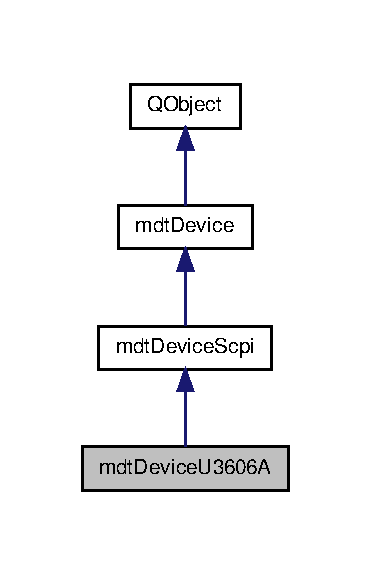
\includegraphics[width=178pt]{classmdt_device_u3606_a__inherit__graph}
\end{center}
\end{figure}


Collaboration diagram for mdt\-Device\-U3606\-A\-:
\nopagebreak
\begin{figure}[H]
\begin{center}
\leavevmode
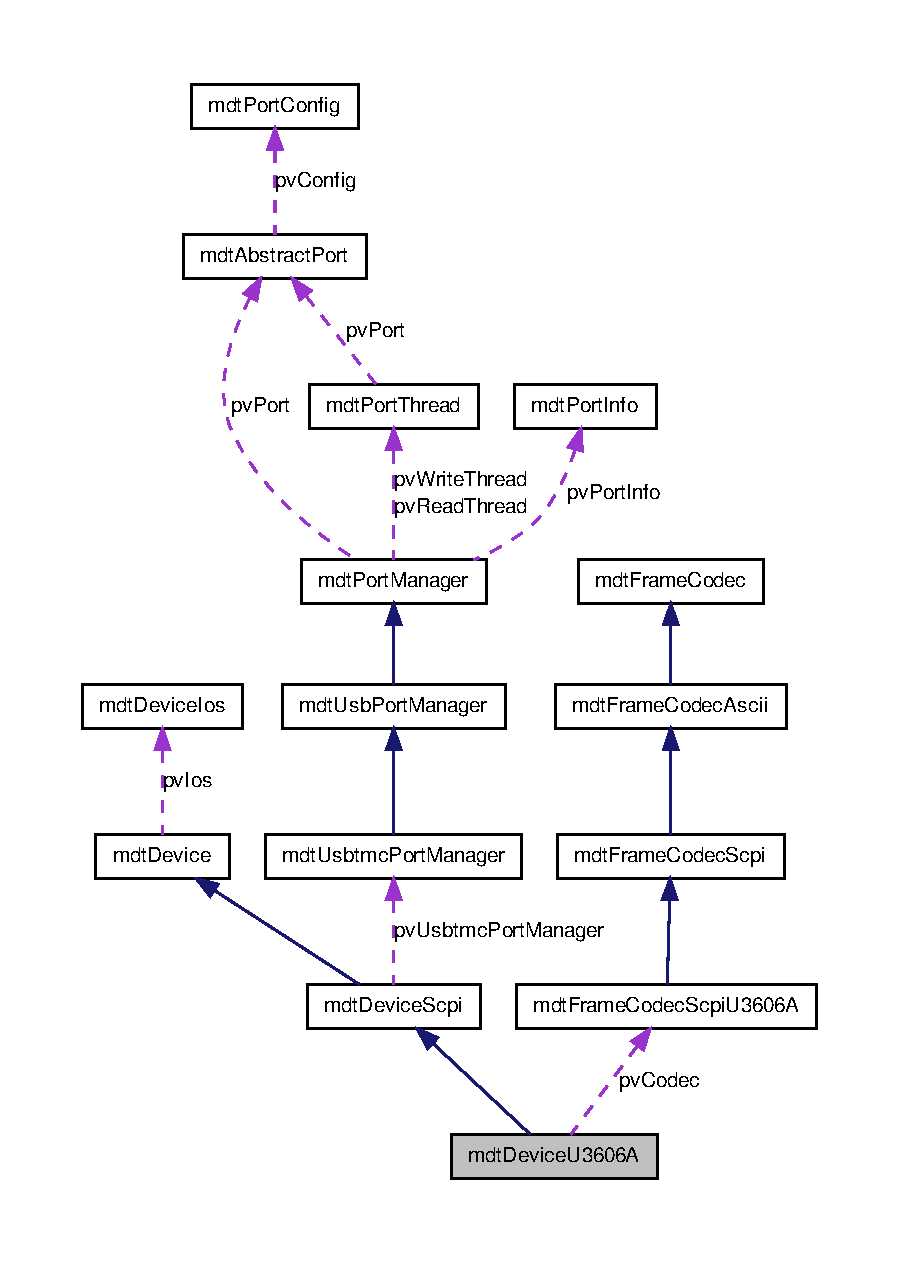
\includegraphics[width=350pt]{classmdt_device_u3606_a__coll__graph}
\end{center}
\end{figure}
\subsection*{Public Types}
\begin{DoxyCompactItemize}
\item 
enum \hyperlink{classmdt_device_u3606_a_ae05c254d19a66c1728d30100f7c600dc}{range\-\_\-t} \{ \\*
\hyperlink{classmdt_device_u3606_a_ae05c254d19a66c1728d30100f7c600dcaad020d13863dbfcb395ce08330d5724e}{Range\-Auto} = -\/10, 
\hyperlink{classmdt_device_u3606_a_ae05c254d19a66c1728d30100f7c600dca7a11a8189a61ead1b631c06488bb8a06}{Range\-Min}, 
\hyperlink{classmdt_device_u3606_a_ae05c254d19a66c1728d30100f7c600dcaea44e09b32e699856e6dd58c0a222344}{Range\-Max}, 
\hyperlink{classmdt_device_u3606_a_ae05c254d19a66c1728d30100f7c600dca724e28864e513d31ac8a9c3525a0a5aa}{Range100} = 1, 
\\*
\hyperlink{classmdt_device_u3606_a_ae05c254d19a66c1728d30100f7c600dca7c08dab5ef9ed34a00304f8aa0b8f17f}{Range1k}, 
\hyperlink{classmdt_device_u3606_a_ae05c254d19a66c1728d30100f7c600dca50d29071b501dc633b5a12fac4f23a53}{Range10k}, 
\hyperlink{classmdt_device_u3606_a_ae05c254d19a66c1728d30100f7c600dca4baa02141d972c77f493a53691bae435}{Range100k}, 
\hyperlink{classmdt_device_u3606_a_ae05c254d19a66c1728d30100f7c600dcacd7e52976fffc3eb6def4efb5303d082}{Range1\-M}, 
\\*
\hyperlink{classmdt_device_u3606_a_ae05c254d19a66c1728d30100f7c600dcadf4218b4809f09c734ee289fbfc06108}{Range10\-M}, 
\hyperlink{classmdt_device_u3606_a_ae05c254d19a66c1728d30100f7c600dca20e91ee2eeb1a64e2353586c8c8b3cea}{Range100\-M}
 \}
\begin{DoxyCompactList}\small\item\em Range. \end{DoxyCompactList}\item 
enum \hyperlink{classmdt_device_u3606_a_a1899206163f2a0163d09cbc482daf806}{resolution\-\_\-t} \{ \hyperlink{classmdt_device_u3606_a_a1899206163f2a0163d09cbc482daf806a49419daba75cbb553401b066a3c2e6da}{Resolution\-Min}, 
\hyperlink{classmdt_device_u3606_a_a1899206163f2a0163d09cbc482daf806a82c71d88404eb70e505cbce753aaf06f}{Resolution\-Max}
 \}
\begin{DoxyCompactList}\small\item\em Resolution. \end{DoxyCompactList}\end{DoxyCompactItemize}
\subsection*{Public Slots}
\begin{DoxyCompactItemize}
\item 
void \hyperlink{classmdt_device_u3606_a_a94a6f8b3f64cd35b33204c66816f3f6a}{on\-State\-Changed} (int state)
\begin{DoxyCompactList}\small\item\em Update (G)U\-I when device's state has changed. \end{DoxyCompactList}\end{DoxyCompactItemize}
\subsection*{Public Member Functions}
\begin{DoxyCompactItemize}
\item 
\hyperlink{classmdt_device_u3606_a_a91201ae14df7b553a947b5857eaa1c65}{mdt\-Device\-U3606\-A} (\hyperlink{class_q_object}{Q\-Object} $\ast$parent=0)
\begin{DoxyCompactList}\small\item\em Constructor. \end{DoxyCompactList}\item 
\hyperlink{classmdt_device_u3606_a_a7d2fb26475e72cce95ca6be384d569b7}{$\sim$mdt\-Device\-U3606\-A} ()
\begin{DoxyCompactList}\small\item\em Destructor. \end{DoxyCompactList}\item 
\hyperlink{classmdt_abstract_port_ad4121bb930c95887e77f8bafa065a85e}{mdt\-Abstract\-Port\-::error\-\_\-t} \hyperlink{classmdt_device_u3606_a_acf3b48b13bc179ad4f94b3011b7d607a}{connect\-To\-Device} (const \hyperlink{classmdt_device_info}{mdt\-Device\-Info} \&dev\-Info)
\begin{DoxyCompactList}\small\item\em Search and connect to physical device. \end{DoxyCompactList}\item 
int \hyperlink{classmdt_device_u3606_a_a3ccd18368d0c1a2641e209a471e5753e}{setup\-Resistance\-Measure} (\hyperlink{classmdt_device_u3606_a_ae05c254d19a66c1728d30100f7c600dc}{range\-\_\-t} range, \hyperlink{classmdt_device_u3606_a_a1899206163f2a0163d09cbc482daf806}{resolution\-\_\-t} resolution)
\begin{DoxyCompactList}\small\item\em Setup resistance measure. \end{DoxyCompactList}\item 
\hyperlink{classmdt_frame_codec_scpi_u3606_a_a3d7a1de14d77797a08e3d2991fa9f004}{mdt\-Frame\-Codec\-Scpi\-U3606\-A\-::measure\-\_\-type\-\_\-t} \hyperlink{classmdt_device_u3606_a_a8732ec3f4a04a191585191e1ba4f190d}{get\-Measure\-Configuration} ()
\begin{DoxyCompactList}\small\item\em Get the measure configuration. \end{DoxyCompactList}\item 
\hyperlink{classmdt_value}{mdt\-Value} \hyperlink{classmdt_device_u3606_a_ae75a1a896f905487d080761a2b8cf5a5}{get\-Measure\-Value} ()
\begin{DoxyCompactList}\small\item\em Get measure value. \end{DoxyCompactList}\end{DoxyCompactItemize}
\subsection*{Additional Inherited Members}


\subsection{Detailed Description}
Representation of a Agilent U3606\-A. 

The U3606\-A has following I/\-Os

\begin{TabularC}{4}
\hline
\rowcolor{lightgray}{\bf Type}&{\bf Address}&{\bf Label short}&{\bf Description }\\\cline{1-4}
Analog input&0&M\-E\-A\-S\-U\-R\-E&Represent the measurement part \\\cline{1-4}
Analog input&1&S\-E\-N\-S\-E\-U&Represent the voltage sense of the source part \\\cline{1-4}
Analog input&2&S\-E\-N\-S\-E\-I&Represent the current sense of the source part \\\cline{1-4}
Analog output&0&S\-O\-U\-R\-C\-E&Represent the source part \\\cline{1-4}
\end{TabularC}


Definition at line 42 of file mdt\-Device\-U3606\-A.\-h.



\subsection{Member Enumeration Documentation}
\hypertarget{classmdt_device_u3606_a_ae05c254d19a66c1728d30100f7c600dc}{\index{mdt\-Device\-U3606\-A@{mdt\-Device\-U3606\-A}!range\-\_\-t@{range\-\_\-t}}
\index{range\-\_\-t@{range\-\_\-t}!mdtDeviceU3606A@{mdt\-Device\-U3606\-A}}
\subsubsection[{range\-\_\-t}]{\setlength{\rightskip}{0pt plus 5cm}enum {\bf mdt\-Device\-U3606\-A\-::range\-\_\-t}}}\label{classmdt_device_u3606_a_ae05c254d19a66c1728d30100f7c600dc}


Range. 

\begin{Desc}
\item[Enumerator]\par
\begin{description}
\index{Range\-Auto@{Range\-Auto}!mdt\-Device\-U3606\-A@{mdt\-Device\-U3606\-A}}\index{mdt\-Device\-U3606\-A@{mdt\-Device\-U3606\-A}!Range\-Auto@{Range\-Auto}}\item[{\em 
\hypertarget{classmdt_device_u3606_a_ae05c254d19a66c1728d30100f7c600dcaad020d13863dbfcb395ce08330d5724e}{Range\-Auto}\label{classmdt_device_u3606_a_ae05c254d19a66c1728d30100f7c600dcaad020d13863dbfcb395ce08330d5724e}
}]A\-U\-T\-O range \index{Range\-Min@{Range\-Min}!mdt\-Device\-U3606\-A@{mdt\-Device\-U3606\-A}}\index{mdt\-Device\-U3606\-A@{mdt\-Device\-U3606\-A}!Range\-Min@{Range\-Min}}\item[{\em 
\hypertarget{classmdt_device_u3606_a_ae05c254d19a66c1728d30100f7c600dca7a11a8189a61ead1b631c06488bb8a06}{Range\-Min}\label{classmdt_device_u3606_a_ae05c254d19a66c1728d30100f7c600dca7a11a8189a61ead1b631c06488bb8a06}
}]M\-I\-N range \index{Range\-Max@{Range\-Max}!mdt\-Device\-U3606\-A@{mdt\-Device\-U3606\-A}}\index{mdt\-Device\-U3606\-A@{mdt\-Device\-U3606\-A}!Range\-Max@{Range\-Max}}\item[{\em 
\hypertarget{classmdt_device_u3606_a_ae05c254d19a66c1728d30100f7c600dcaea44e09b32e699856e6dd58c0a222344}{Range\-Max}\label{classmdt_device_u3606_a_ae05c254d19a66c1728d30100f7c600dcaea44e09b32e699856e6dd58c0a222344}
}]M\-A\-X range \index{Range100@{Range100}!mdt\-Device\-U3606\-A@{mdt\-Device\-U3606\-A}}\index{mdt\-Device\-U3606\-A@{mdt\-Device\-U3606\-A}!Range100@{Range100}}\item[{\em 
\hypertarget{classmdt_device_u3606_a_ae05c254d19a66c1728d30100f7c600dca724e28864e513d31ac8a9c3525a0a5aa}{Range100}\label{classmdt_device_u3606_a_ae05c254d19a66c1728d30100f7c600dca724e28864e513d31ac8a9c3525a0a5aa}
}]100 range \index{Range1k@{Range1k}!mdt\-Device\-U3606\-A@{mdt\-Device\-U3606\-A}}\index{mdt\-Device\-U3606\-A@{mdt\-Device\-U3606\-A}!Range1k@{Range1k}}\item[{\em 
\hypertarget{classmdt_device_u3606_a_ae05c254d19a66c1728d30100f7c600dca7c08dab5ef9ed34a00304f8aa0b8f17f}{Range1k}\label{classmdt_device_u3606_a_ae05c254d19a66c1728d30100f7c600dca7c08dab5ef9ed34a00304f8aa0b8f17f}
}]1k range \index{Range10k@{Range10k}!mdt\-Device\-U3606\-A@{mdt\-Device\-U3606\-A}}\index{mdt\-Device\-U3606\-A@{mdt\-Device\-U3606\-A}!Range10k@{Range10k}}\item[{\em 
\hypertarget{classmdt_device_u3606_a_ae05c254d19a66c1728d30100f7c600dca50d29071b501dc633b5a12fac4f23a53}{Range10k}\label{classmdt_device_u3606_a_ae05c254d19a66c1728d30100f7c600dca50d29071b501dc633b5a12fac4f23a53}
}]10k range \index{Range100k@{Range100k}!mdt\-Device\-U3606\-A@{mdt\-Device\-U3606\-A}}\index{mdt\-Device\-U3606\-A@{mdt\-Device\-U3606\-A}!Range100k@{Range100k}}\item[{\em 
\hypertarget{classmdt_device_u3606_a_ae05c254d19a66c1728d30100f7c600dca4baa02141d972c77f493a53691bae435}{Range100k}\label{classmdt_device_u3606_a_ae05c254d19a66c1728d30100f7c600dca4baa02141d972c77f493a53691bae435}
}]100k range \index{Range1\-M@{Range1\-M}!mdt\-Device\-U3606\-A@{mdt\-Device\-U3606\-A}}\index{mdt\-Device\-U3606\-A@{mdt\-Device\-U3606\-A}!Range1\-M@{Range1\-M}}\item[{\em 
\hypertarget{classmdt_device_u3606_a_ae05c254d19a66c1728d30100f7c600dcacd7e52976fffc3eb6def4efb5303d082}{Range1\-M}\label{classmdt_device_u3606_a_ae05c254d19a66c1728d30100f7c600dcacd7e52976fffc3eb6def4efb5303d082}
}]1\-M range \index{Range10\-M@{Range10\-M}!mdt\-Device\-U3606\-A@{mdt\-Device\-U3606\-A}}\index{mdt\-Device\-U3606\-A@{mdt\-Device\-U3606\-A}!Range10\-M@{Range10\-M}}\item[{\em 
\hypertarget{classmdt_device_u3606_a_ae05c254d19a66c1728d30100f7c600dcadf4218b4809f09c734ee289fbfc06108}{Range10\-M}\label{classmdt_device_u3606_a_ae05c254d19a66c1728d30100f7c600dcadf4218b4809f09c734ee289fbfc06108}
}]10\-M range \index{Range100\-M@{Range100\-M}!mdt\-Device\-U3606\-A@{mdt\-Device\-U3606\-A}}\index{mdt\-Device\-U3606\-A@{mdt\-Device\-U3606\-A}!Range100\-M@{Range100\-M}}\item[{\em 
\hypertarget{classmdt_device_u3606_a_ae05c254d19a66c1728d30100f7c600dca20e91ee2eeb1a64e2353586c8c8b3cea}{Range100\-M}\label{classmdt_device_u3606_a_ae05c254d19a66c1728d30100f7c600dca20e91ee2eeb1a64e2353586c8c8b3cea}
}]100\-M range \end{description}
\end{Desc}


Definition at line 50 of file mdt\-Device\-U3606\-A.\-h.

\hypertarget{classmdt_device_u3606_a_a1899206163f2a0163d09cbc482daf806}{\index{mdt\-Device\-U3606\-A@{mdt\-Device\-U3606\-A}!resolution\-\_\-t@{resolution\-\_\-t}}
\index{resolution\-\_\-t@{resolution\-\_\-t}!mdtDeviceU3606A@{mdt\-Device\-U3606\-A}}
\subsubsection[{resolution\-\_\-t}]{\setlength{\rightskip}{0pt plus 5cm}enum {\bf mdt\-Device\-U3606\-A\-::resolution\-\_\-t}}}\label{classmdt_device_u3606_a_a1899206163f2a0163d09cbc482daf806}


Resolution. 

\begin{Desc}
\item[Enumerator]\par
\begin{description}
\index{Resolution\-Min@{Resolution\-Min}!mdt\-Device\-U3606\-A@{mdt\-Device\-U3606\-A}}\index{mdt\-Device\-U3606\-A@{mdt\-Device\-U3606\-A}!Resolution\-Min@{Resolution\-Min}}\item[{\em 
\hypertarget{classmdt_device_u3606_a_a1899206163f2a0163d09cbc482daf806a49419daba75cbb553401b066a3c2e6da}{Resolution\-Min}\label{classmdt_device_u3606_a_a1899206163f2a0163d09cbc482daf806a49419daba75cbb553401b066a3c2e6da}
}]5 1/2 digit \index{Resolution\-Max@{Resolution\-Max}!mdt\-Device\-U3606\-A@{mdt\-Device\-U3606\-A}}\index{mdt\-Device\-U3606\-A@{mdt\-Device\-U3606\-A}!Resolution\-Max@{Resolution\-Max}}\item[{\em 
\hypertarget{classmdt_device_u3606_a_a1899206163f2a0163d09cbc482daf806a82c71d88404eb70e505cbce753aaf06f}{Resolution\-Max}\label{classmdt_device_u3606_a_a1899206163f2a0163d09cbc482daf806a82c71d88404eb70e505cbce753aaf06f}
}]4 1/2 digit \end{description}
\end{Desc}


Definition at line 65 of file mdt\-Device\-U3606\-A.\-h.



\subsection{Constructor \& Destructor Documentation}
\hypertarget{classmdt_device_u3606_a_a91201ae14df7b553a947b5857eaa1c65}{\index{mdt\-Device\-U3606\-A@{mdt\-Device\-U3606\-A}!mdt\-Device\-U3606\-A@{mdt\-Device\-U3606\-A}}
\index{mdt\-Device\-U3606\-A@{mdt\-Device\-U3606\-A}!mdtDeviceU3606A@{mdt\-Device\-U3606\-A}}
\subsubsection[{mdt\-Device\-U3606\-A}]{\setlength{\rightskip}{0pt plus 5cm}mdt\-Device\-U3606\-A\-::mdt\-Device\-U3606\-A (
\begin{DoxyParamCaption}
\item[{{\bf Q\-Object} $\ast$}]{parent = {\ttfamily 0}}
\end{DoxyParamCaption}
)}}\label{classmdt_device_u3606_a_a91201ae14df7b553a947b5857eaa1c65}


Constructor. 

Will create the needed codec, I/\-Os and configure internal port manager . 

Definition at line 31 of file mdt\-Device\-U3606\-A.\-cpp.



References mdt\-Device\-::add\-Input(), mdt\-Device\-::add\-Output(), mdt\-Port\-Manager\-::config(), mdt\-Device\-Scpi\-::port\-Manager(), mdt\-Device\-Scpi\-::pv\-Usbtmc\-Port\-Manager, mdt\-Abstract\-Io\-::set\-Address(), mdt\-Abstract\-Io\-::set\-Label\-Short(), mdt\-Port\-Config\-::set\-Read\-Frame\-Size(), mdt\-Port\-Config\-::set\-Read\-Queue\-Size(), mdt\-Port\-Config\-::set\-Read\-Timeout(), mdt\-Port\-Config\-::set\-Write\-Frame\-Size(), and mdt\-Port\-Config\-::set\-Write\-Queue\-Size().

\hypertarget{classmdt_device_u3606_a_a7d2fb26475e72cce95ca6be384d569b7}{\index{mdt\-Device\-U3606\-A@{mdt\-Device\-U3606\-A}!$\sim$mdt\-Device\-U3606\-A@{$\sim$mdt\-Device\-U3606\-A}}
\index{$\sim$mdt\-Device\-U3606\-A@{$\sim$mdt\-Device\-U3606\-A}!mdtDeviceU3606A@{mdt\-Device\-U3606\-A}}
\subsubsection[{$\sim$mdt\-Device\-U3606\-A}]{\setlength{\rightskip}{0pt plus 5cm}mdt\-Device\-U3606\-A\-::$\sim$mdt\-Device\-U3606\-A (
\begin{DoxyParamCaption}
{}
\end{DoxyParamCaption}
)}}\label{classmdt_device_u3606_a_a7d2fb26475e72cce95ca6be384d569b7}


Destructor. 



Definition at line 63 of file mdt\-Device\-U3606\-A.\-cpp.



\subsection{Member Function Documentation}
\hypertarget{classmdt_device_u3606_a_acf3b48b13bc179ad4f94b3011b7d607a}{\index{mdt\-Device\-U3606\-A@{mdt\-Device\-U3606\-A}!connect\-To\-Device@{connect\-To\-Device}}
\index{connect\-To\-Device@{connect\-To\-Device}!mdtDeviceU3606A@{mdt\-Device\-U3606\-A}}
\subsubsection[{connect\-To\-Device}]{\setlength{\rightskip}{0pt plus 5cm}{\bf mdt\-Abstract\-Port\-::error\-\_\-t} mdt\-Device\-U3606\-A\-::connect\-To\-Device (
\begin{DoxyParamCaption}
\item[{const {\bf mdt\-Device\-Info} \&}]{dev\-Info}
\end{DoxyParamCaption}
)\hspace{0.3cm}{\ttfamily [virtual]}}}\label{classmdt_device_u3606_a_acf3b48b13bc179ad4f94b3011b7d607a}


Search and connect to physical device. 

Will scan available ports and open the first port that has device attached maching request.


\begin{DoxyParams}{Parameters}
{\em dev\-Info} & Requested device's informations. Note\-: Vendor I\-D and/or product I\-D are automatically set. (in other words, a empty \hyperlink{classmdt_device_info}{mdt\-Device\-Info} can be passed). Optionnaly, a serial I\-D can be set (usefull if many U3606\-A devices are connected) \\
\hline
\end{DoxyParams}
\begin{DoxyReturn}{Returns}
A error listed in \hyperlink{classmdt_abstract_port_ad4121bb930c95887e77f8bafa065a85e}{mdt\-Abstract\-Port\-::error\-\_\-t} (No\-Error on success) 
\end{DoxyReturn}


Reimplemented from \hyperlink{classmdt_device_scpi_ae8e886b362cbf9d1bf7064b48348b8e8}{mdt\-Device\-Scpi}.



Definition at line 68 of file mdt\-Device\-U3606\-A.\-cpp.



References mdt\-Device\-Scpi\-::connect\-To\-Device(), mdt\-Device\-Info\-::set\-Product\-Id(), and mdt\-Device\-Info\-::set\-Vendor\-Id().

\hypertarget{classmdt_device_u3606_a_a8732ec3f4a04a191585191e1ba4f190d}{\index{mdt\-Device\-U3606\-A@{mdt\-Device\-U3606\-A}!get\-Measure\-Configuration@{get\-Measure\-Configuration}}
\index{get\-Measure\-Configuration@{get\-Measure\-Configuration}!mdtDeviceU3606A@{mdt\-Device\-U3606\-A}}
\subsubsection[{get\-Measure\-Configuration}]{\setlength{\rightskip}{0pt plus 5cm}{\bf mdt\-Frame\-Codec\-Scpi\-U3606\-A\-::measure\-\_\-type\-\_\-t} mdt\-Device\-U3606\-A\-::get\-Measure\-Configuration (
\begin{DoxyParamCaption}
{}
\end{DoxyParamCaption}
)}}\label{classmdt_device_u3606_a_a8732ec3f4a04a191585191e1ba4f190d}


Get the measure configuration. 

Will get the device current measure configuration by sending the C\-O\-N\-F? query .

Internal analog measure input is also updated with device's range and unit .

By error, unknown measure type is returned . 

Definition at line 146 of file mdt\-Device\-U3606\-A.\-cpp.



References mdt\-Device\-::get\-New\-Transaction(), mdt\-Frame\-Codec\-Scpi\-U3606\-A\-::measure\-Type(), mdt\-Frame\-Codec\-Scpi\-U3606\-A\-::\-M\-T\-\_\-\-U\-N\-K\-N\-O\-W, mdt\-Device\-Scpi\-::port\-Manager(), mdt\-Frame\-Codec\-Scpi\-::\-Q\-T\-\_\-\-C\-O\-N\-F, mdt\-Usbtmc\-Port\-Manager\-::send\-Data(), mdt\-Usbtmc\-Port\-Manager\-::send\-Read\-Request(), mdt\-Port\-Transaction\-::set\-Query\-Reply\-Mode(), mdt\-Port\-Transaction\-::set\-Type(), and mdt\-Device\-::wait\-Transaction\-Done().

\hypertarget{classmdt_device_u3606_a_ae75a1a896f905487d080761a2b8cf5a5}{\index{mdt\-Device\-U3606\-A@{mdt\-Device\-U3606\-A}!get\-Measure\-Value@{get\-Measure\-Value}}
\index{get\-Measure\-Value@{get\-Measure\-Value}!mdtDeviceU3606A@{mdt\-Device\-U3606\-A}}
\subsubsection[{get\-Measure\-Value}]{\setlength{\rightskip}{0pt plus 5cm}{\bf mdt\-Value} mdt\-Device\-U3606\-A\-::get\-Measure\-Value (
\begin{DoxyParamCaption}
{}
\end{DoxyParamCaption}
)}}\label{classmdt_device_u3606_a_ae75a1a896f905487d080761a2b8cf5a5}


Get measure value. 

This is similar to call get\-Analog\-Input\-Value(\char`\"{}\-M\-E\-A\-S\-U\-R\-E\char`\"{}, true, true) . 

Definition at line 177 of file mdt\-Device\-U3606\-A.\-cpp.



References mdt\-Device\-::get\-Analog\-Input\-Value().

\hypertarget{classmdt_device_u3606_a_a94a6f8b3f64cd35b33204c66816f3f6a}{\index{mdt\-Device\-U3606\-A@{mdt\-Device\-U3606\-A}!on\-State\-Changed@{on\-State\-Changed}}
\index{on\-State\-Changed@{on\-State\-Changed}!mdtDeviceU3606A@{mdt\-Device\-U3606\-A}}
\subsubsection[{on\-State\-Changed}]{\setlength{\rightskip}{0pt plus 5cm}void mdt\-Device\-U3606\-A\-::on\-State\-Changed (
\begin{DoxyParamCaption}
\item[{int}]{state}
\end{DoxyParamCaption}
)\hspace{0.3cm}{\ttfamily [slot]}}}\label{classmdt_device_u3606_a_a94a6f8b3f64cd35b33204c66816f3f6a}


Update (G)U\-I when device's state has changed. 



Definition at line 182 of file mdt\-Device\-U3606\-A.\-cpp.

\hypertarget{classmdt_device_u3606_a_a3ccd18368d0c1a2641e209a471e5753e}{\index{mdt\-Device\-U3606\-A@{mdt\-Device\-U3606\-A}!setup\-Resistance\-Measure@{setup\-Resistance\-Measure}}
\index{setup\-Resistance\-Measure@{setup\-Resistance\-Measure}!mdtDeviceU3606A@{mdt\-Device\-U3606\-A}}
\subsubsection[{setup\-Resistance\-Measure}]{\setlength{\rightskip}{0pt plus 5cm}int mdt\-Device\-U3606\-A\-::setup\-Resistance\-Measure (
\begin{DoxyParamCaption}
\item[{{\bf mdt\-Device\-U3606\-A\-::range\-\_\-t}}]{range, }
\item[{{\bf mdt\-Device\-U3606\-A\-::resolution\-\_\-t}}]{resolution}
\end{DoxyParamCaption}
)}}\label{classmdt_device_u3606_a_a3ccd18368d0c1a2641e209a471e5753e}


Setup resistance measure. 


\begin{DoxyParams}{Parameters}
{\em range} & If range is supported by instrument, it will be set, else A\-U\-T\-O range is used. \\
\hline
{\em resolution} & Resolution to use \\
\hline
\end{DoxyParams}
\begin{DoxyReturn}{Returns}
Value $<$ 0 on error, $>$= 0 on success 
\end{DoxyReturn}


Definition at line 80 of file mdt\-Device\-U3606\-A.\-cpp.



References mdt\-Error\-::commit(), mdt\-Error\-::\-Error, M\-D\-T\-\_\-\-E\-R\-R\-O\-R\-\_\-\-S\-E\-T\-\_\-\-S\-R\-C, mdt\-Device\-::name(), mdt\-Device\-::pv\-Last\-Error, Range100, Range100k, Range100\-M, Range10k, Range10\-M, Range1k, Range1\-M, Range\-Auto, Range\-Max, Range\-Min, Resolution\-Max, Resolution\-Min, mdt\-Device\-Scpi\-::send\-Command(), mdt\-Error\-::set\-Error(), and mdt\-Error\-::\-Warning.



The documentation for this class was generated from the following files\-:\begin{DoxyCompactItemize}
\item 
src/mdtdevice/\hyperlink{mdt_device_u3606_a_8h}{mdt\-Device\-U3606\-A.\-h}\item 
src/mdtdevice/\hyperlink{mdt_device_u3606_a_8cpp}{mdt\-Device\-U3606\-A.\-cpp}\end{DoxyCompactItemize}

\hypertarget{classmdt_device_u3606_a_widget}{\section{mdt\-Device\-U3606\-A\-Widget Class Reference}
\label{classmdt_device_u3606_a_widget}\index{mdt\-Device\-U3606\-A\-Widget@{mdt\-Device\-U3606\-A\-Widget}}
}


{\ttfamily \#include $<$mdt\-Device\-U3606\-A\-Widget.\-h$>$}



Inheritance diagram for mdt\-Device\-U3606\-A\-Widget\-:\nopagebreak
\begin{figure}[H]
\begin{center}
\leavevmode
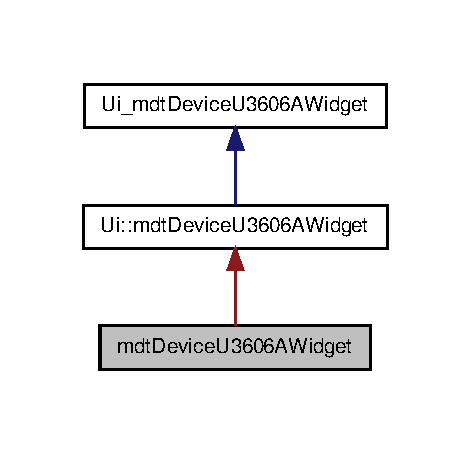
\includegraphics[width=298pt]{classmdt_device_u3606_a_widget__inherit__graph}
\end{center}
\end{figure}


Collaboration diagram for mdt\-Device\-U3606\-A\-Widget\-:\nopagebreak
\begin{figure}[H]
\begin{center}
\leavevmode
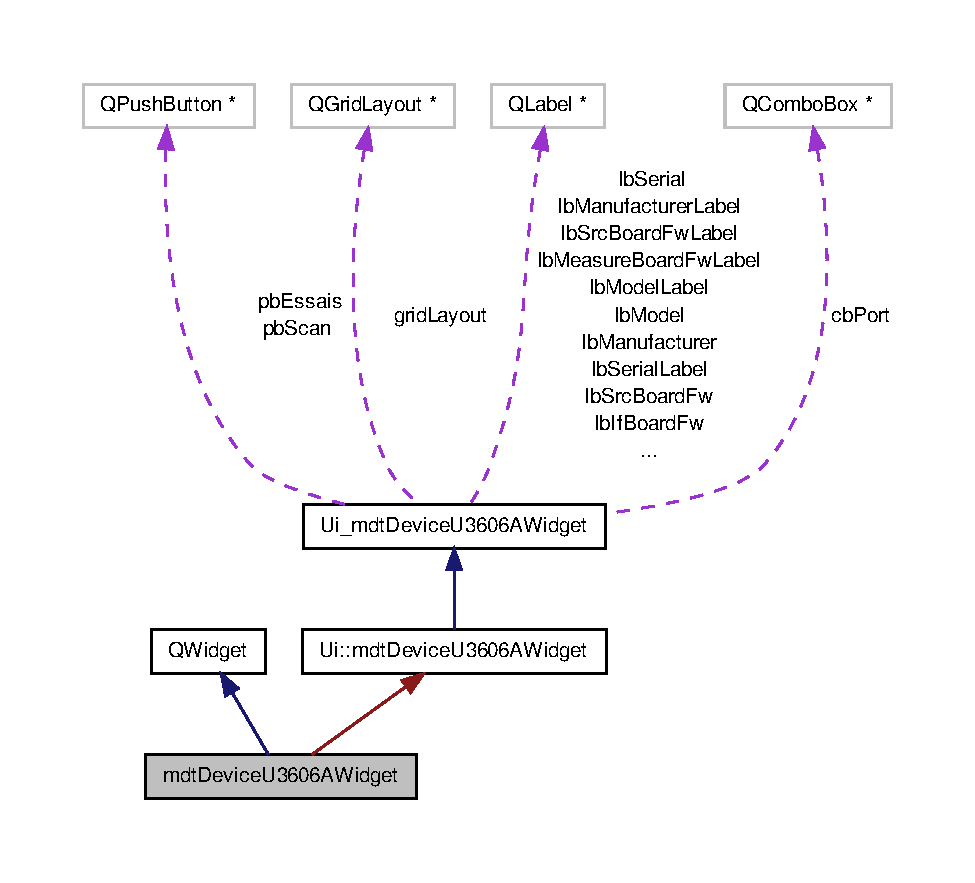
\includegraphics[width=350pt]{classmdt_device_u3606_a_widget__coll__graph}
\end{center}
\end{figure}
\subsection*{Public Slots}
\begin{DoxyCompactItemize}
\item 
void \hyperlink{classmdt_device_u3606_a_widget_aa232cf25e8ac0dee00cde5089af623b0}{essais} ()
\item 
void \hyperlink{classmdt_device_u3606_a_widget_abc2b2860e71a9c79af6697205ead2a84}{scan} ()
\item 
void \hyperlink{classmdt_device_u3606_a_widget_a15409aed9aa73929b64be63db9f31f8e}{select\-Port} (const Q\-String \&port)
\item 
void \hyperlink{classmdt_device_u3606_a_widget_a3e979d85d5e198a97b36b4956d06ce8e}{display\-Idn} (const Q\-String\-List \&data)
\end{DoxyCompactItemize}
\subsection*{Public Member Functions}
\begin{DoxyCompactItemize}
\item 
\hyperlink{classmdt_device_u3606_a_widget_a653d85749d67555d8c3a43a779b6d2a2}{mdt\-Device\-U3606\-A\-Widget} (\hyperlink{class_q_widget}{Q\-Widget} $\ast$parent=0)
\end{DoxyCompactItemize}
\subsection*{Additional Inherited Members}


\subsection{Detailed Description}
\begin{DoxyRefDesc}{Todo}
\item[\hyperlink{todo__todo000009}{Todo}]A supprimer !(?)! \end{DoxyRefDesc}


Definition at line 32 of file mdt\-Device\-U3606\-A\-Widget.\-h.



\subsection{Constructor \& Destructor Documentation}
\hypertarget{classmdt_device_u3606_a_widget_a653d85749d67555d8c3a43a779b6d2a2}{\index{mdt\-Device\-U3606\-A\-Widget@{mdt\-Device\-U3606\-A\-Widget}!mdt\-Device\-U3606\-A\-Widget@{mdt\-Device\-U3606\-A\-Widget}}
\index{mdt\-Device\-U3606\-A\-Widget@{mdt\-Device\-U3606\-A\-Widget}!mdtDeviceU3606AWidget@{mdt\-Device\-U3606\-A\-Widget}}
\subsubsection[{mdt\-Device\-U3606\-A\-Widget}]{\setlength{\rightskip}{0pt plus 5cm}mdt\-Device\-U3606\-A\-Widget\-::mdt\-Device\-U3606\-A\-Widget (
\begin{DoxyParamCaption}
\item[{{\bf Q\-Widget} $\ast$}]{parent = {\ttfamily 0}}
\end{DoxyParamCaption}
)}}\label{classmdt_device_u3606_a_widget_a653d85749d67555d8c3a43a779b6d2a2}
\begin{DoxyRefDesc}{Todo}
\item[\hyperlink{todo__todo000008}{Todo}]A supprimer !(?)! \end{DoxyRefDesc}


Definition at line 27 of file mdt\-Device\-U3606\-A\-Widget.\-cpp.



References Ui\-\_\-mdt\-Device\-U3606\-A\-Widget\-::cb\-Port, display\-Idn(), essais(), Ui\-\_\-mdt\-Device\-U3606\-A\-Widget\-::pb\-Essais, Ui\-\_\-mdt\-Device\-U3606\-A\-Widget\-::pb\-Scan, scan(), select\-Port(), and Ui\-\_\-mdt\-Device\-U3606\-A\-Widget\-::setup\-Ui().



\subsection{Member Function Documentation}
\hypertarget{classmdt_device_u3606_a_widget_a3e979d85d5e198a97b36b4956d06ce8e}{\index{mdt\-Device\-U3606\-A\-Widget@{mdt\-Device\-U3606\-A\-Widget}!display\-Idn@{display\-Idn}}
\index{display\-Idn@{display\-Idn}!mdtDeviceU3606AWidget@{mdt\-Device\-U3606\-A\-Widget}}
\subsubsection[{display\-Idn}]{\setlength{\rightskip}{0pt plus 5cm}void mdt\-Device\-U3606\-A\-Widget\-::display\-Idn (
\begin{DoxyParamCaption}
\item[{const Q\-String\-List \&}]{data}
\end{DoxyParamCaption}
)\hspace{0.3cm}{\ttfamily [slot]}}}\label{classmdt_device_u3606_a_widget_a3e979d85d5e198a97b36b4956d06ce8e}


Definition at line 73 of file mdt\-Device\-U3606\-A\-Widget.\-cpp.



References Ui\-\_\-mdt\-Device\-U3606\-A\-Widget\-::lb\-If\-Board\-Fw, Ui\-\_\-mdt\-Device\-U3606\-A\-Widget\-::lb\-Manufacturer, Ui\-\_\-mdt\-Device\-U3606\-A\-Widget\-::lb\-Measure\-Board\-Fw, Ui\-\_\-mdt\-Device\-U3606\-A\-Widget\-::lb\-Model, Ui\-\_\-mdt\-Device\-U3606\-A\-Widget\-::lb\-Serial, and Ui\-\_\-mdt\-Device\-U3606\-A\-Widget\-::lb\-Src\-Board\-Fw.



Referenced by mdt\-Device\-U3606\-A\-Widget().

\hypertarget{classmdt_device_u3606_a_widget_aa232cf25e8ac0dee00cde5089af623b0}{\index{mdt\-Device\-U3606\-A\-Widget@{mdt\-Device\-U3606\-A\-Widget}!essais@{essais}}
\index{essais@{essais}!mdtDeviceU3606AWidget@{mdt\-Device\-U3606\-A\-Widget}}
\subsubsection[{essais}]{\setlength{\rightskip}{0pt plus 5cm}void mdt\-Device\-U3606\-A\-Widget\-::essais (
\begin{DoxyParamCaption}
{}
\end{DoxyParamCaption}
)\hspace{0.3cm}{\ttfamily [slot]}}}\label{classmdt_device_u3606_a_widget_aa232cf25e8ac0dee00cde5089af623b0}


Definition at line 42 of file mdt\-Device\-U3606\-A\-Widget.\-cpp.



References Ui\-\_\-mdt\-Device\-U3606\-A\-Widget\-::pb\-Essais.



Referenced by mdt\-Device\-U3606\-A\-Widget().

\hypertarget{classmdt_device_u3606_a_widget_abc2b2860e71a9c79af6697205ead2a84}{\index{mdt\-Device\-U3606\-A\-Widget@{mdt\-Device\-U3606\-A\-Widget}!scan@{scan}}
\index{scan@{scan}!mdtDeviceU3606AWidget@{mdt\-Device\-U3606\-A\-Widget}}
\subsubsection[{scan}]{\setlength{\rightskip}{0pt plus 5cm}void mdt\-Device\-U3606\-A\-Widget\-::scan (
\begin{DoxyParamCaption}
{}
\end{DoxyParamCaption}
)\hspace{0.3cm}{\ttfamily [slot]}}}\label{classmdt_device_u3606_a_widget_abc2b2860e71a9c79af6697205ead2a84}


Definition at line 50 of file mdt\-Device\-U3606\-A\-Widget.\-cpp.



References Ui\-\_\-mdt\-Device\-U3606\-A\-Widget\-::cb\-Port, and Ui\-\_\-mdt\-Device\-U3606\-A\-Widget\-::pb\-Scan.



Referenced by mdt\-Device\-U3606\-A\-Widget().

\hypertarget{classmdt_device_u3606_a_widget_a15409aed9aa73929b64be63db9f31f8e}{\index{mdt\-Device\-U3606\-A\-Widget@{mdt\-Device\-U3606\-A\-Widget}!select\-Port@{select\-Port}}
\index{select\-Port@{select\-Port}!mdtDeviceU3606AWidget@{mdt\-Device\-U3606\-A\-Widget}}
\subsubsection[{select\-Port}]{\setlength{\rightskip}{0pt plus 5cm}void mdt\-Device\-U3606\-A\-Widget\-::select\-Port (
\begin{DoxyParamCaption}
\item[{const Q\-String \&}]{port}
\end{DoxyParamCaption}
)\hspace{0.3cm}{\ttfamily [slot]}}}\label{classmdt_device_u3606_a_widget_a15409aed9aa73929b64be63db9f31f8e}


Definition at line 58 of file mdt\-Device\-U3606\-A\-Widget.\-cpp.



References Ui\-\_\-mdt\-Device\-U3606\-A\-Widget\-::pb\-Essais.



Referenced by mdt\-Device\-U3606\-A\-Widget().



The documentation for this class was generated from the following files\-:\begin{DoxyCompactItemize}
\item 
src/mdtdevice/linux/\hyperlink{mdt_device_u3606_a_widget_8h}{mdt\-Device\-U3606\-A\-Widget.\-h}\item 
src/mdtdevice/linux/\hyperlink{mdt_device_u3606_a_widget_8cpp}{mdt\-Device\-U3606\-A\-Widget.\-cpp}\end{DoxyCompactItemize}

\hypertarget{classmdt_error}{
\section{mdtError Class Reference}
\label{classmdt_error}\index{mdtError@{mdtError}}
}


\hyperlink{classmdt_error}{mdtError} contains informations about a error that occured  




{\ttfamily \#include $<$mdtError.h$>$}

\subsection*{Public Types}
\begin{DoxyCompactItemize}
\item 
enum \hyperlink{classmdt_error_a5c8b1a040e2feaa848f6201d6b6f0cd7}{level\_\-t} \{ \hyperlink{classmdt_error_a5c8b1a040e2feaa848f6201d6b6f0cd7a1ba619a7f332d8fe18fb3cd270ff86eb}{NoError} =  0x00, 
\hyperlink{classmdt_error_a5c8b1a040e2feaa848f6201d6b6f0cd7a24688d5f5af0a3a54636fa1a4b2f60fc}{Info} =  0x01, 
\hyperlink{classmdt_error_a5c8b1a040e2feaa848f6201d6b6f0cd7a61d92805e90226faf3d1c5fd350a0ab8}{Warning} =  0x02, 
\hyperlink{classmdt_error_a5c8b1a040e2feaa848f6201d6b6f0cd7a35f5c05a7d15b6433445cdbffa6d5260}{Error} =  0x04
 \}
\begin{DoxyCompactList}\small\item\em Error level. \end{DoxyCompactList}\end{DoxyCompactItemize}
\subsection*{Public Member Functions}
\begin{DoxyCompactItemize}
\item 
\hypertarget{classmdt_error_a78824dc8c0029107949baaf28c4a9df5}{
\hyperlink{classmdt_error_a78824dc8c0029107949baaf28c4a9df5}{mdtError} ()}
\label{classmdt_error_a78824dc8c0029107949baaf28c4a9df5}

\begin{DoxyCompactList}\small\item\em Constructor. \end{DoxyCompactList}\item 
\hyperlink{classmdt_error_a377c175cc8e1aeae543cae2ecc5ca87b}{mdtError} (int number, const QString \&text, \hyperlink{classmdt_error_a5c8b1a040e2feaa848f6201d6b6f0cd7}{level\_\-t} level)
\begin{DoxyCompactList}\small\item\em Construct new error. \end{DoxyCompactList}\item 
\hypertarget{classmdt_error_a775542a251ef746f3433e7d790a48d85}{
\hyperlink{classmdt_error_a775542a251ef746f3433e7d790a48d85}{mdtError} (const QString \&text, \hyperlink{classmdt_error_a5c8b1a040e2feaa848f6201d6b6f0cd7}{level\_\-t} level)}
\label{classmdt_error_a775542a251ef746f3433e7d790a48d85}

\begin{DoxyCompactList}\small\item\em Construct new error. \end{DoxyCompactList}\item 
void \hyperlink{classmdt_error_a8e7961a665841c1b052116e4dd2eb855}{setError} (const QString \&text, \hyperlink{classmdt_error_a5c8b1a040e2feaa848f6201d6b6f0cd7}{level\_\-t} level)
\begin{DoxyCompactList}\small\item\em Set error. \end{DoxyCompactList}\item 
\hypertarget{classmdt_error_a9fa7eb879fe7b26c4a4f0bd55fe29ffa}{
void \hyperlink{classmdt_error_a9fa7eb879fe7b26c4a4f0bd55fe29ffa}{clear} ()}
\label{classmdt_error_a9fa7eb879fe7b26c4a4f0bd55fe29ffa}

\begin{DoxyCompactList}\small\item\em Clear. \end{DoxyCompactList}\item 
\hypertarget{classmdt_error_a49254fdb566fee1a4adafe6a3694befc}{
void \hyperlink{classmdt_error_a49254fdb566fee1a4adafe6a3694befc}{setSystemError} (int number, const QString \&text)}
\label{classmdt_error_a49254fdb566fee1a4adafe6a3694befc}

\begin{DoxyCompactList}\small\item\em Add system returned error (for example, errno) \end{DoxyCompactList}\item 
void \hyperlink{classmdt_error_a8dd3203e11b308e6c2701d7f075af885}{setSource} (const QString \&filePath, int fileLine, const QString \&className, const QString \&functionName)
\begin{DoxyCompactList}\small\item\em Add system error (for Windows API) \end{DoxyCompactList}\item 
\hypertarget{classmdt_error_ad3cccf7c7f7d4bdabdcb4e60794bb9cb}{
void \hyperlink{classmdt_error_ad3cccf7c7f7d4bdabdcb4e60794bb9cb}{commit} ()}
\label{classmdt_error_ad3cccf7c7f7d4bdabdcb4e60794bb9cb}

\begin{DoxyCompactList}\small\item\em Send error to output. \end{DoxyCompactList}\item 
int \hyperlink{classmdt_error_ad233adb8efe4180b85f584c5afdd49fc}{number} () const 
\begin{DoxyCompactList}\small\item\em Error number. \end{DoxyCompactList}\item 
\hypertarget{classmdt_error_a8630bb6b21b70edfe3d13eaff82a1baf}{
QString \hyperlink{classmdt_error_a8630bb6b21b70edfe3d13eaff82a1baf}{text} () const }
\label{classmdt_error_a8630bb6b21b70edfe3d13eaff82a1baf}

\begin{DoxyCompactList}\small\item\em Error text. \end{DoxyCompactList}\item 
\hypertarget{classmdt_error_a8d8382d3008de890689df415deb7766e}{
\hyperlink{classmdt_error_a5c8b1a040e2feaa848f6201d6b6f0cd7}{level\_\-t} \hyperlink{classmdt_error_a8d8382d3008de890689df415deb7766e}{level} () const }
\label{classmdt_error_a8d8382d3008de890689df415deb7766e}

\begin{DoxyCompactList}\small\item\em Error level  level\_\-t. \end{DoxyCompactList}\item 
\hypertarget{classmdt_error_aac5a7cec9a5d4364f9331c80e1eafe99}{
QMessageBox::Icon \hyperlink{classmdt_error_aac5a7cec9a5d4364f9331c80e1eafe99}{levelIcon} () const }
\label{classmdt_error_aac5a7cec9a5d4364f9331c80e1eafe99}

\begin{DoxyCompactList}\small\item\em Map the level to a QMessageBox Icon. \end{DoxyCompactList}\item 
\hypertarget{classmdt_error_a1be3f45cd56b3142f50c288df9f53204}{
int \hyperlink{classmdt_error_a1be3f45cd56b3142f50c288df9f53204}{systemNumber} () const }
\label{classmdt_error_a1be3f45cd56b3142f50c288df9f53204}

\begin{DoxyCompactList}\small\item\em Error number returned from system if available. \end{DoxyCompactList}\item 
\hypertarget{classmdt_error_a6cd449e657f321b86d234269b5e92cda}{
QString \hyperlink{classmdt_error_a6cd449e657f321b86d234269b5e92cda}{systemText} () const }
\label{classmdt_error_a6cd449e657f321b86d234269b5e92cda}

\begin{DoxyCompactList}\small\item\em Error text returned from system, if available. \end{DoxyCompactList}\item 
QString \hyperlink{classmdt_error_a28d22c0b9341faacfef22a7deae2da3c}{systemErrorString} (QObject $\ast$obj=0) const 
\begin{DoxyCompactList}\small\item\em Error number and text from system, if available. \end{DoxyCompactList}\item 
\hypertarget{classmdt_error_a8ef108a0502df7875f1b54bbb2a8919d}{
void \hyperlink{classmdt_error_a8ef108a0502df7875f1b54bbb2a8919d}{setInformativeText} (const QString \&text)}
\label{classmdt_error_a8ef108a0502df7875f1b54bbb2a8919d}

\begin{DoxyCompactList}\small\item\em Set informative text. \end{DoxyCompactList}\item 
\hypertarget{classmdt_error_adcc1905f585c327cec8a2e31af616651}{
QString \hyperlink{classmdt_error_adcc1905f585c327cec8a2e31af616651}{informativeText} () const }
\label{classmdt_error_adcc1905f585c327cec8a2e31af616651}

\begin{DoxyCompactList}\small\item\em Get informative text. \end{DoxyCompactList}\item 
\hypertarget{classmdt_error_abff9bc71ff554f6f6189be88b0afa731}{
QString \hyperlink{classmdt_error_abff9bc71ff554f6f6189be88b0afa731}{functionName} () const }
\label{classmdt_error_abff9bc71ff554f6f6189be88b0afa731}

\begin{DoxyCompactList}\small\item\em Error source function. \end{DoxyCompactList}\item 
\hypertarget{classmdt_error_af7c2c371678ebd45698a990502addbd8}{
QString \hyperlink{classmdt_error_af7c2c371678ebd45698a990502addbd8}{fileName} () const }
\label{classmdt_error_af7c2c371678ebd45698a990502addbd8}

\begin{DoxyCompactList}\small\item\em Error source file (name only) \end{DoxyCompactList}\item 
\hypertarget{classmdt_error_a7f5a9ac5e896ba24009bcadddcfe79cb}{
int \hyperlink{classmdt_error_a7f5a9ac5e896ba24009bcadddcfe79cb}{fileLine} () const }
\label{classmdt_error_a7f5a9ac5e896ba24009bcadddcfe79cb}

\begin{DoxyCompactList}\small\item\em Error source line. \end{DoxyCompactList}\end{DoxyCompactItemize}


\subsection{Detailed Description}
\hyperlink{classmdt_error}{mdtError} contains informations about a error that occured 

Currently, a \hyperlink{classmdt_error}{mdtError} contains several informations:
\begin{DoxyItemize}
\item text (mandatory) : a description of the error that occured . Access: \hyperlink{classmdt_error_a775542a251ef746f3433e7d790a48d85}{mdtError(const QString\&, level\_\-t)} , \hyperlink{classmdt_error_a8630bb6b21b70edfe3d13eaff82a1baf}{text()} .
\item level (mandatory) : the severity of the error . Access: \hyperlink{classmdt_error_a775542a251ef746f3433e7d790a48d85}{mdtError(const QString\&, level\_\-t)} , \hyperlink{classmdt_error_a8d8382d3008de890689df415deb7766e}{level()} , \hyperlink{classmdt_error_aac5a7cec9a5d4364f9331c80e1eafe99}{levelIcon()} .
\item systemNumber (optional) : error number returned by a system (or other library) call . Access: \hyperlink{classmdt_error_a49254fdb566fee1a4adafe6a3694befc}{setSystemError()} , \hyperlink{classmdt_error_a1be3f45cd56b3142f50c288df9f53204}{systemNumber()} , \hyperlink{classmdt_error_a28d22c0b9341faacfef22a7deae2da3c}{systemErrorString()} .
\item systemText (optional) : error text number returned by a system (or other library) call . Access: \hyperlink{classmdt_error_a49254fdb566fee1a4adafe6a3694befc}{setSystemError()} , \hyperlink{classmdt_error_a6cd449e657f321b86d234269b5e92cda}{systemText()} , \hyperlink{classmdt_error_a28d22c0b9341faacfef22a7deae2da3c}{systemErrorString()} .
\item informativeText (optional) : can be used the same way than QMessageBox . Access : \hyperlink{classmdt_error_a8ef108a0502df7875f1b54bbb2a8919d}{setInformativeText()} , \hyperlink{classmdt_error_adcc1905f585c327cec8a2e31af616651}{informativeText()} .
\end{DoxyItemize}

number : currently used with mdt\_\-error\_\-t enum, but it seems that this is not a good idea, and this will change once a better one is found ...

This class contains the information of a error. To just put it to standard defined outputs, use \hyperlink{classmdt_error_ad3cccf7c7f7d4bdabdcb4e60794bb9cb}{commit()} .

Note: no copy constrctor/operator are defined, because only primitve and copiable objects are used, but a \hyperlink{classmdt_error}{mdtError} can be copied . 

Definition at line 84 of file mdtError.h.



\subsection{Member Enumeration Documentation}
\hypertarget{classmdt_error_a5c8b1a040e2feaa848f6201d6b6f0cd7}{
\index{mdtError@{mdtError}!level\_\-t@{level\_\-t}}
\index{level\_\-t@{level\_\-t}!mdtError@{mdtError}}
\subsubsection[{level\_\-t}]{\setlength{\rightskip}{0pt plus 5cm}enum {\bf mdtError::level\_\-t}}}
\label{classmdt_error_a5c8b1a040e2feaa848f6201d6b6f0cd7}


Error level. 

\begin{Desc}
\item[Enumerator: ]\par
\begin{description}
\index{NoError@{NoError}!mdtError@{mdtError}}\index{mdtError@{mdtError}!NoError@{NoError}}\item[{\em 
\hypertarget{classmdt_error_a5c8b1a040e2feaa848f6201d6b6f0cd7a1ba619a7f332d8fe18fb3cd270ff86eb}{
NoError}
\label{classmdt_error_a5c8b1a040e2feaa848f6201d6b6f0cd7a1ba619a7f332d8fe18fb3cd270ff86eb}
}]No error . \index{Info@{Info}!mdtError@{mdtError}}\index{mdtError@{mdtError}!Info@{Info}}\item[{\em 
\hypertarget{classmdt_error_a5c8b1a040e2feaa848f6201d6b6f0cd7a24688d5f5af0a3a54636fa1a4b2f60fc}{
Info}
\label{classmdt_error_a5c8b1a040e2feaa848f6201d6b6f0cd7a24688d5f5af0a3a54636fa1a4b2f60fc}
}]Just a information, application continues to work in normal way . \index{Warning@{Warning}!mdtError@{mdtError}}\index{mdtError@{mdtError}!Warning@{Warning}}\item[{\em 
\hypertarget{classmdt_error_a5c8b1a040e2feaa848f6201d6b6f0cd7a61d92805e90226faf3d1c5fd350a0ab8}{
Warning}
\label{classmdt_error_a5c8b1a040e2feaa848f6201d6b6f0cd7a61d92805e90226faf3d1c5fd350a0ab8}
}]Error that could be handled \index{Error@{Error}!mdtError@{mdtError}}\index{mdtError@{mdtError}!Error@{Error}}\item[{\em 
\hypertarget{classmdt_error_a5c8b1a040e2feaa848f6201d6b6f0cd7a35f5c05a7d15b6433445cdbffa6d5260}{
Error}
\label{classmdt_error_a5c8b1a040e2feaa848f6201d6b6f0cd7a35f5c05a7d15b6433445cdbffa6d5260}
}]Error that was not handled \end{description}
\end{Desc}



Definition at line 90 of file mdtError.h.



\subsection{Constructor \& Destructor Documentation}
\hypertarget{classmdt_error_a377c175cc8e1aeae543cae2ecc5ca87b}{
\index{mdtError@{mdtError}!mdtError@{mdtError}}
\index{mdtError@{mdtError}!mdtError@{mdtError}}
\subsubsection[{mdtError}]{\setlength{\rightskip}{0pt plus 5cm}mdtError::mdtError (
\begin{DoxyParamCaption}
\item[{int}]{number, }
\item[{const QString \&}]{text, }
\item[{{\bf mdtError::level\_\-t}}]{level}
\end{DoxyParamCaption}
)}}
\label{classmdt_error_a377c175cc8e1aeae543cae2ecc5ca87b}


Construct new error. 

\begin{Desc}
\item[\hyperlink{deprecated__deprecated000001}{Deprecated}]If no good idea falls in for the usage of number , this constrctor should become obselete . \end{Desc}


Definition at line 34 of file mdtError.cpp.



\subsection{Member Function Documentation}
\hypertarget{classmdt_error_ad233adb8efe4180b85f584c5afdd49fc}{
\index{mdtError@{mdtError}!number@{number}}
\index{number@{number}!mdtError@{mdtError}}
\subsubsection[{number}]{\setlength{\rightskip}{0pt plus 5cm}int mdtError::number (
\begin{DoxyParamCaption}
{}
\end{DoxyParamCaption}
) const}}
\label{classmdt_error_ad233adb8efe4180b85f584c5afdd49fc}


Error number. 

\begin{Desc}
\item[\hyperlink{deprecated__deprecated000002}{Deprecated}]If no good idea falls in for the usage of number , this method should become obselete . \end{Desc}


Definition at line 113 of file mdtError.cpp.

\hypertarget{classmdt_error_a8e7961a665841c1b052116e4dd2eb855}{
\index{mdtError@{mdtError}!setError@{setError}}
\index{setError@{setError}!mdtError@{mdtError}}
\subsubsection[{setError}]{\setlength{\rightskip}{0pt plus 5cm}void mdtError::setError (
\begin{DoxyParamCaption}
\item[{const QString \&}]{text, }
\item[{{\bf level\_\-t}}]{level}
\end{DoxyParamCaption}
)}}
\label{classmdt_error_a8e7961a665841c1b052116e4dd2eb855}


Set error. 

Will also clear current error . 

Definition at line 58 of file mdtError.cpp.

\hypertarget{classmdt_error_a8dd3203e11b308e6c2701d7f075af885}{
\index{mdtError@{mdtError}!setSource@{setSource}}
\index{setSource@{setSource}!mdtError@{mdtError}}
\subsubsection[{setSource}]{\setlength{\rightskip}{0pt plus 5cm}void mdtError::setSource (
\begin{DoxyParamCaption}
\item[{const QString \&}]{filePath, }
\item[{int}]{fileLine, }
\item[{const QString \&}]{className, }
\item[{const QString \&}]{functionName}
\end{DoxyParamCaption}
)}}
\label{classmdt_error_a8dd3203e11b308e6c2701d7f075af885}


Add system error (for Windows API) 

When using Windows API, the standard mechanism is GetLastError() and FormatMessage(). Calling this method will do this internally.

Add the source of error

It's possible to use the helper macro MDT\_\-ERROR\_\-SET\_\-SRC() 

Definition at line 96 of file mdtError.cpp.

\hypertarget{classmdt_error_a28d22c0b9341faacfef22a7deae2da3c}{
\index{mdtError@{mdtError}!systemErrorString@{systemErrorString}}
\index{systemErrorString@{systemErrorString}!mdtError@{mdtError}}
\subsubsection[{systemErrorString}]{\setlength{\rightskip}{0pt plus 5cm}QString mdtError::systemErrorString (
\begin{DoxyParamCaption}
\item[{QObject $\ast$}]{obj = {\ttfamily 0}}
\end{DoxyParamCaption}
) const}}
\label{classmdt_error_a28d22c0b9341faacfef22a7deae2da3c}


Error number and text from system, if available. 

If obj is set, translation is used. (We not want to use the static QObject::tr() ). 

Definition at line 153 of file mdtError.cpp.



The documentation for this class was generated from the following files:\begin{DoxyCompactItemize}
\item 
src/mdtutils/mdtError.h\item 
src/mdtutils/mdtError.cpp\end{DoxyCompactItemize}

\hypertarget{classmdt_error_out}{\section{mdt\-Error\-Out Class Reference}
\label{classmdt_error_out}\index{mdt\-Error\-Out@{mdt\-Error\-Out}}
}


Error output system Helper for error output. Outputs are the stderr output (console), a G\-U\-I messagebox and a logfile.  




{\ttfamily \#include $<$mdt\-Error\-Out.\-h$>$}



Inheritance diagram for mdt\-Error\-Out\-:\nopagebreak
\begin{figure}[H]
\begin{center}
\leavevmode
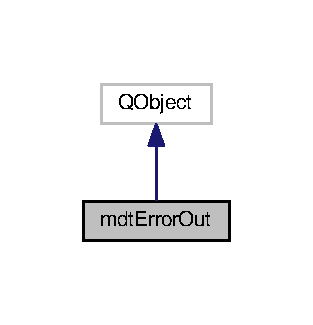
\includegraphics[width=150pt]{classmdt_error_out__inherit__graph}
\end{center}
\end{figure}


Collaboration diagram for mdt\-Error\-Out\-:\nopagebreak
\begin{figure}[H]
\begin{center}
\leavevmode
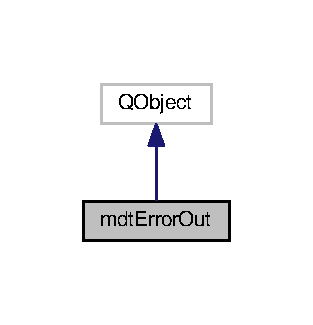
\includegraphics[width=150pt]{classmdt_error_out__coll__graph}
\end{center}
\end{figure}
\subsection*{Signals}
\begin{DoxyCompactItemize}
\item 
void \hyperlink{classmdt_error_out_a033747841ec3340f0396e574723095d7}{sig\-Show\-Dialog} (\hyperlink{classmdt_error}{mdt\-Error} error)
\end{DoxyCompactItemize}
\subsection*{Static Public Member Functions}
\begin{DoxyCompactItemize}
\item 
static bool \hyperlink{classmdt_error_out_a9c7f05b03d0f09ff02e8f747bdcd1de7}{init} (const Q\-String \&\hyperlink{classmdt_error_out_a22f721fff4d6368a4a3d51279c6af8fa}{log\-File})
\begin{DoxyCompactList}\small\item\em Initialize the error output system. \end{DoxyCompactList}\item 
static void \hyperlink{classmdt_error_out_a547e4e8aa75528710e4a17e9faf48621}{set\-Log\-Levels\-Mask} (int mask)
\begin{DoxyCompactList}\small\item\em Set the log levels mask. \end{DoxyCompactList}\item 
static void \hyperlink{classmdt_error_out_afa76bdf497b750829277566ec07d44d8}{set\-Dialog\-Levels\-Mask} (int mask)
\begin{DoxyCompactList}\small\item\em Set the dialog display levels mask. \end{DoxyCompactList}\item 
static void \hyperlink{classmdt_error_out_aeb562e93216b34e7b73aa69f42065895}{add\-Error} (\hyperlink{classmdt_error}{mdt\-Error} \&error)
\begin{DoxyCompactList}\small\item\em Add a error to the error output system. \end{DoxyCompactList}\item 
static \hyperlink{classmdt_error_out}{mdt\-Error\-Out} $\ast$ \hyperlink{classmdt_error_out_a7a80480a61ca1a2704ec16d69647f739}{instance} ()
\begin{DoxyCompactList}\small\item\em Get the instance of the error output system. \end{DoxyCompactList}\item 
static Q\-String \hyperlink{classmdt_error_out_a22f721fff4d6368a4a3d51279c6af8fa}{log\-File} ()
\begin{DoxyCompactList}\small\item\em Get the log file path. \end{DoxyCompactList}\item 
static void \hyperlink{classmdt_error_out_a45c1370762b47a06ec597d6e89ebc73d}{destroy} ()
\begin{DoxyCompactList}\small\item\em Destroy the error output system instance. \end{DoxyCompactList}\item 
static void \hyperlink{classmdt_error_out_afd7f41eaf7e07b4fceb83297e9040e35}{set\-Log\-File\-Max\-Size} (qint64 max\-Size)
\begin{DoxyCompactList}\small\item\em Set the maximum log file size \mbox{[}Byte\mbox{]} before backup. \end{DoxyCompactList}\end{DoxyCompactItemize}


\subsection{Detailed Description}
Error output system Helper for error output. Outputs are the stderr output (console), a G\-U\-I messagebox and a logfile. 

Definition at line 38 of file mdt\-Error\-Out.\-h.



\subsection{Member Function Documentation}
\hypertarget{classmdt_error_out_aeb562e93216b34e7b73aa69f42065895}{\index{mdt\-Error\-Out@{mdt\-Error\-Out}!add\-Error@{add\-Error}}
\index{add\-Error@{add\-Error}!mdtErrorOut@{mdt\-Error\-Out}}
\subsubsection[{add\-Error}]{\setlength{\rightskip}{0pt plus 5cm}void mdt\-Error\-Out\-::add\-Error (
\begin{DoxyParamCaption}
\item[{{\bf mdt\-Error} \&}]{error}
\end{DoxyParamCaption}
)\hspace{0.3cm}{\ttfamily [static]}}}\label{classmdt_error_out_aeb562e93216b34e7b73aa69f42065895}


Add a error to the error output system. 

\begin{DoxyPrecond}{Precondition}
The system must be initialized.
\end{DoxyPrecond}
\begin{DoxySeeAlso}{See Also}
\hyperlink{classmdt_error_out_a9c7f05b03d0f09ff02e8f747bdcd1de7}{init()} 
\end{DoxySeeAlso}


Definition at line 93 of file mdt\-Error\-Out.\-cpp.



References mdt\-Error\-::\-Error, mdt\-Error\-::file\-Line(), mdt\-Error\-::file\-Name(), mdt\-Error\-::function\-Name(), mdt\-Error\-::\-Info, instance(), mdt\-Error\-::level(), mdt\-Error\-::number(), mdt\-Error\-Out\-Logger\-::put\-Data(), sig\-Show\-Dialog(), mdt\-Error\-::system\-Number(), mdt\-Error\-::system\-Text(), mdt\-Error\-::text(), and mdt\-Error\-::\-Warning.



Referenced by mdt\-Error\-::commit().

\hypertarget{classmdt_error_out_a45c1370762b47a06ec597d6e89ebc73d}{\index{mdt\-Error\-Out@{mdt\-Error\-Out}!destroy@{destroy}}
\index{destroy@{destroy}!mdtErrorOut@{mdt\-Error\-Out}}
\subsubsection[{destroy}]{\setlength{\rightskip}{0pt plus 5cm}void mdt\-Error\-Out\-::destroy (
\begin{DoxyParamCaption}
{}
\end{DoxyParamCaption}
)\hspace{0.3cm}{\ttfamily [static]}}}\label{classmdt_error_out_a45c1370762b47a06ec597d6e89ebc73d}


Destroy the error output system instance. 

This function must be called from main thread (G\-U\-I thread) 

Definition at line 184 of file mdt\-Error\-Out.\-cpp.



Referenced by main(), and mdt\-Application\-::$\sim$mdt\-Application().

\hypertarget{classmdt_error_out_a9c7f05b03d0f09ff02e8f747bdcd1de7}{\index{mdt\-Error\-Out@{mdt\-Error\-Out}!init@{init}}
\index{init@{init}!mdtErrorOut@{mdt\-Error\-Out}}
\subsubsection[{init}]{\setlength{\rightskip}{0pt plus 5cm}bool mdt\-Error\-Out\-::init (
\begin{DoxyParamCaption}
\item[{const Q\-String \&}]{log\-File}
\end{DoxyParamCaption}
)\hspace{0.3cm}{\ttfamily [static]}}}\label{classmdt_error_out_a9c7f05b03d0f09ff02e8f747bdcd1de7}


Initialize the error output system. 

After this call, the log and dialog levels are defined to Warning and Error This function must be called from main thread (G\-U\-I thread) 

Definition at line 56 of file mdt\-Error\-Out.\-cpp.



References instance(), mdt\-Error\-Out\-Logger\-::set\-Log\-File\-Path(), and sig\-Show\-Dialog().



Referenced by mdt\-Application\-::init(), and main().

\hypertarget{classmdt_error_out_a7a80480a61ca1a2704ec16d69647f739}{\index{mdt\-Error\-Out@{mdt\-Error\-Out}!instance@{instance}}
\index{instance@{instance}!mdtErrorOut@{mdt\-Error\-Out}}
\subsubsection[{instance}]{\setlength{\rightskip}{0pt plus 5cm}{\bf mdt\-Error\-Out} $\ast$ mdt\-Error\-Out\-::instance (
\begin{DoxyParamCaption}
{}
\end{DoxyParamCaption}
)\hspace{0.3cm}{\ttfamily [static]}}}\label{classmdt_error_out_a7a80480a61ca1a2704ec16d69647f739}


Get the instance of the error output system. 

This function can return a Null pointer if \hyperlink{classmdt_error_out_a9c7f05b03d0f09ff02e8f747bdcd1de7}{init()} was never called. This function, and returned pointer, should be used with care in multi-\/thread applicatopn ! 

Definition at line 170 of file mdt\-Error\-Out.\-cpp.



Referenced by add\-Error(), init(), log\-File(), set\-Dialog\-Levels\-Mask(), set\-Log\-File\-Max\-Size(), and set\-Log\-Levels\-Mask().

\hypertarget{classmdt_error_out_a22f721fff4d6368a4a3d51279c6af8fa}{\index{mdt\-Error\-Out@{mdt\-Error\-Out}!log\-File@{log\-File}}
\index{log\-File@{log\-File}!mdtErrorOut@{mdt\-Error\-Out}}
\subsubsection[{log\-File}]{\setlength{\rightskip}{0pt plus 5cm}Q\-String mdt\-Error\-Out\-::log\-File (
\begin{DoxyParamCaption}
{}
\end{DoxyParamCaption}
)\hspace{0.3cm}{\ttfamily [static]}}}\label{classmdt_error_out_a22f721fff4d6368a4a3d51279c6af8fa}


Get the log file path. 

\begin{DoxyPrecond}{Precondition}
The system must be initialized.
\end{DoxyPrecond}
\begin{DoxySeeAlso}{See Also}
\hyperlink{classmdt_error_out_a9c7f05b03d0f09ff02e8f747bdcd1de7}{init()} 
\end{DoxySeeAlso}


Definition at line 175 of file mdt\-Error\-Out.\-cpp.



References instance(), and mdt\-Error\-Out\-Logger\-::log\-File\-Path().

\hypertarget{classmdt_error_out_afa76bdf497b750829277566ec07d44d8}{\index{mdt\-Error\-Out@{mdt\-Error\-Out}!set\-Dialog\-Levels\-Mask@{set\-Dialog\-Levels\-Mask}}
\index{set\-Dialog\-Levels\-Mask@{set\-Dialog\-Levels\-Mask}!mdtErrorOut@{mdt\-Error\-Out}}
\subsubsection[{set\-Dialog\-Levels\-Mask}]{\setlength{\rightskip}{0pt plus 5cm}void mdt\-Error\-Out\-::set\-Dialog\-Levels\-Mask (
\begin{DoxyParamCaption}
\item[{int}]{mask}
\end{DoxyParamCaption}
)\hspace{0.3cm}{\ttfamily [static]}}}\label{classmdt_error_out_afa76bdf497b750829277566ec07d44d8}


Set the dialog display levels mask. 

The mask is a O\-R combinaison of \hyperlink{classmdt_error_a5c8b1a040e2feaa848f6201d6b6f0cd7}{mdt\-Error\-::level\-\_\-t} flags \begin{DoxyPrecond}{Precondition}
The system must be initialized.
\end{DoxyPrecond}
\begin{DoxySeeAlso}{See Also}
\hyperlink{classmdt_error_out_a9c7f05b03d0f09ff02e8f747bdcd1de7}{init()} 
\end{DoxySeeAlso}


Definition at line 84 of file mdt\-Error\-Out.\-cpp.



References instance().



Referenced by mdt\-Application\-::init(), and main().

\hypertarget{classmdt_error_out_afd7f41eaf7e07b4fceb83297e9040e35}{\index{mdt\-Error\-Out@{mdt\-Error\-Out}!set\-Log\-File\-Max\-Size@{set\-Log\-File\-Max\-Size}}
\index{set\-Log\-File\-Max\-Size@{set\-Log\-File\-Max\-Size}!mdtErrorOut@{mdt\-Error\-Out}}
\subsubsection[{set\-Log\-File\-Max\-Size}]{\setlength{\rightskip}{0pt plus 5cm}void mdt\-Error\-Out\-::set\-Log\-File\-Max\-Size (
\begin{DoxyParamCaption}
\item[{qint64}]{max\-Size}
\end{DoxyParamCaption}
)\hspace{0.3cm}{\ttfamily [static]}}}\label{classmdt_error_out_afd7f41eaf7e07b4fceb83297e9040e35}


Set the maximum log file size \mbox{[}Byte\mbox{]} before backup. 



Definition at line 192 of file mdt\-Error\-Out.\-cpp.



References instance(), and mdt\-Error\-Out\-Logger\-::set\-Log\-File\-Max\-Size().

\hypertarget{classmdt_error_out_a547e4e8aa75528710e4a17e9faf48621}{\index{mdt\-Error\-Out@{mdt\-Error\-Out}!set\-Log\-Levels\-Mask@{set\-Log\-Levels\-Mask}}
\index{set\-Log\-Levels\-Mask@{set\-Log\-Levels\-Mask}!mdtErrorOut@{mdt\-Error\-Out}}
\subsubsection[{set\-Log\-Levels\-Mask}]{\setlength{\rightskip}{0pt plus 5cm}void mdt\-Error\-Out\-::set\-Log\-Levels\-Mask (
\begin{DoxyParamCaption}
\item[{int}]{mask}
\end{DoxyParamCaption}
)\hspace{0.3cm}{\ttfamily [static]}}}\label{classmdt_error_out_a547e4e8aa75528710e4a17e9faf48621}


Set the log levels mask. 

The mask is a O\-R combinaison of \hyperlink{classmdt_error_a5c8b1a040e2feaa848f6201d6b6f0cd7}{mdt\-Error\-::level\-\_\-t} flags \begin{DoxyPrecond}{Precondition}
The system must be initialized.
\end{DoxyPrecond}
\begin{DoxySeeAlso}{See Also}
\hyperlink{classmdt_error_out_a9c7f05b03d0f09ff02e8f747bdcd1de7}{init()} 
\end{DoxySeeAlso}


Definition at line 75 of file mdt\-Error\-Out.\-cpp.



References instance().

\hypertarget{classmdt_error_out_a033747841ec3340f0396e574723095d7}{\index{mdt\-Error\-Out@{mdt\-Error\-Out}!sig\-Show\-Dialog@{sig\-Show\-Dialog}}
\index{sig\-Show\-Dialog@{sig\-Show\-Dialog}!mdtErrorOut@{mdt\-Error\-Out}}
\subsubsection[{sig\-Show\-Dialog}]{\setlength{\rightskip}{0pt plus 5cm}void mdt\-Error\-Out\-::sig\-Show\-Dialog (
\begin{DoxyParamCaption}
\item[{{\bf mdt\-Error}}]{error}
\end{DoxyParamCaption}
)\hspace{0.3cm}{\ttfamily [signal]}}}\label{classmdt_error_out_a033747841ec3340f0396e574723095d7}


Definition at line 100 of file moc\-\_\-mdt\-Error\-Out.\-cxx.



Referenced by add\-Error(), and init().



The documentation for this class was generated from the following files\-:\begin{DoxyCompactItemize}
\item 
src/mdtutils/\hyperlink{mdt_error_out_8h}{mdt\-Error\-Out.\-h}\item 
src/mdtutils/\hyperlink{mdt_error_out_8cpp}{mdt\-Error\-Out.\-cpp}\item 
src/mdtutils/\hyperlink{moc__mdt_error_out_8cxx}{moc\-\_\-mdt\-Error\-Out.\-cxx}\end{DoxyCompactItemize}

\hypertarget{classmdt_frame}{
\section{mdtFrame Class Reference}
\label{classmdt_frame}\index{mdtFrame@{mdtFrame}}
}


Provide an array of bytes.  




{\ttfamily \#include $<$mdtFrame.h$>$}



Inheritance diagram for mdtFrame:\nopagebreak
\begin{figure}[H]
\begin{center}
\leavevmode
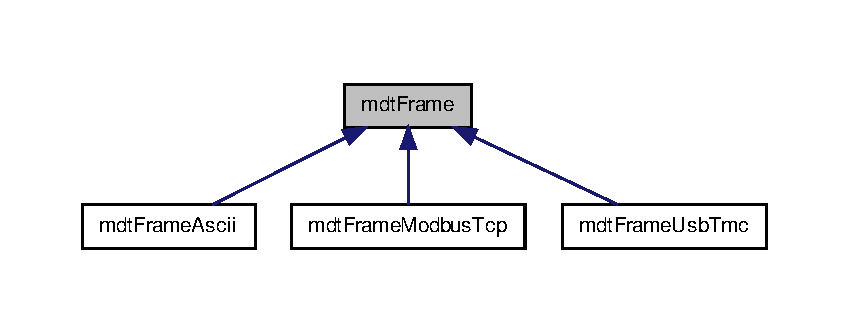
\includegraphics[width=400pt]{classmdt_frame__inherit__graph}
\end{center}
\end{figure}
\subsection*{Public Types}
\begin{DoxyCompactItemize}
\item 
enum \hyperlink{classmdt_frame_af936e37d5fe4c066c0fb0161fafd4a17}{type\_\-t} \{ \par
\hyperlink{classmdt_frame_af936e37d5fe4c066c0fb0161fafd4a17aeb10e33f775c33799273fcb130fee86f}{FT\_\-RAW}, 
\hyperlink{classmdt_frame_af936e37d5fe4c066c0fb0161fafd4a17ac91a1c1827fa634eadaddb861f805c96}{FT\_\-RAW\_\-TOP}, 
\hyperlink{classmdt_frame_af936e37d5fe4c066c0fb0161fafd4a17ac649559564652abbe656b97d4a84b722}{FT\_\-ASCII}, 
\hyperlink{classmdt_frame_af936e37d5fe4c066c0fb0161fafd4a17a72c8ddaf29839f4037b686bdc346828a}{FT\_\-MODBUS\_\-TCP}, 
\par
\hyperlink{classmdt_frame_af936e37d5fe4c066c0fb0161fafd4a17aca438ff6b553a819f22090facc562c86}{FT\_\-USBTMC}
 \}
\begin{DoxyCompactList}\small\item\em Frame type. \end{DoxyCompactList}\end{DoxyCompactItemize}
\subsection*{Public Member Functions}
\begin{DoxyCompactItemize}
\item 
void \hyperlink{classmdt_frame_ac1a8ad77ce7bd6d08032056c3610d5c0}{setIgnoreNullValues} (bool ignoreNullValues)
\begin{DoxyCompactList}\small\item\em Set the ignore null values flag. \end{DoxyCompactList}\item 
int \hyperlink{classmdt_frame_af03d60dadc6bd33b3a333cf484463113}{putUntil} (const char $\ast$data, char token, int maxLen)
\begin{DoxyCompactList}\small\item\em Put data until EOF token was reached. \end{DoxyCompactList}\item 
int \hyperlink{classmdt_frame_aaa5c15df5aaf026b02f34639438036ad}{putUntil} (const char $\ast$data, QByteArray \&token, int maxLen)
\begin{DoxyCompactList}\small\item\em Put data until EOF token was reached. \end{DoxyCompactList}\item 
\hypertarget{classmdt_frame_ab4e0fee7198c94c16f2fa6eb4b6b1562}{
bool \hyperlink{classmdt_frame_ab4e0fee7198c94c16f2fa6eb4b6b1562}{isFull} ()}
\label{classmdt_frame_ab4e0fee7198c94c16f2fa6eb4b6b1562}

\begin{DoxyCompactList}\small\item\em Returns true if frame is full. \end{DoxyCompactList}\item 
\hypertarget{classmdt_frame_aa1cd5c914c36efb3f441b7f6e782dc24}{
int \hyperlink{classmdt_frame_aa1cd5c914c36efb3f441b7f6e782dc24}{remainCapacity} ()}
\label{classmdt_frame_aa1cd5c914c36efb3f441b7f6e782dc24}

\begin{DoxyCompactList}\small\item\em Returns the remain capacity. \end{DoxyCompactList}\item 
int \hyperlink{classmdt_frame_a8526b227a56562fddf8445060e8095d4}{bytesToStore} ()
\begin{DoxyCompactList}\small\item\em Returns the bytes to store into the frame. \end{DoxyCompactList}\item 
void \hyperlink{classmdt_frame_abfd6de396626f01ebf972b7d6cd26957}{setDirectlyComplete} (bool dc)
\begin{DoxyCompactList}\small\item\em Set the complete flag directly. \end{DoxyCompactList}\item 
void \hyperlink{classmdt_frame_ab8db9882c095091109115afb8e448b37}{setComplete} ()
\begin{DoxyCompactList}\small\item\em Set the frame as complete. \end{DoxyCompactList}\item 
\hypertarget{classmdt_frame_a2a8fb9f36c941282881bba0c538d1ce5}{
bool \hyperlink{classmdt_frame_a2a8fb9f36c941282881bba0c538d1ce5}{isComplete} ()}
\label{classmdt_frame_a2a8fb9f36c941282881bba0c538d1ce5}

\begin{DoxyCompactList}\small\item\em Returns true if EOF condition was reached. \end{DoxyCompactList}\item 
void \hyperlink{classmdt_frame_acdf8a921a3f36ca91af88b55b90febdc}{clear} ()
\begin{DoxyCompactList}\small\item\em Overloaded function. \end{DoxyCompactList}\item 
virtual void \hyperlink{classmdt_frame_aecc64d3846dee0049ee7b10b73a402f4}{clearSub} ()
\begin{DoxyCompactList}\small\item\em \hyperlink{classmdt_frame}{mdtFrame} subclass specific clear \end{DoxyCompactList}\item 
virtual int \hyperlink{classmdt_frame_ae63af784d2fc54430ea5db4dc80b7ec8}{putData} (const char $\ast$data, int len)
\begin{DoxyCompactList}\small\item\em Put data into the frame. \end{DoxyCompactList}\item 
virtual int \hyperlink{classmdt_frame_a0e0dcfb9d284ac0dae550db33f0fbece}{eofSeqLen} ()
\begin{DoxyCompactList}\small\item\em Get the length of the end of frame sequence. \end{DoxyCompactList}\item 
int \hyperlink{classmdt_frame_a36e4b85a3c671902ac3c8cc318ca726c}{take} (char $\ast$data, int len)
\begin{DoxyCompactList}\small\item\em Take some data. \end{DoxyCompactList}\item 
int \hyperlink{classmdt_frame_ad8b184e6eb07a26fe84deaf233c1aa9b}{take} (int len)
\begin{DoxyCompactList}\small\item\em Take some data. \end{DoxyCompactList}\item 
void \hyperlink{classmdt_frame_a3b9a331858df9061879592fab1b346f5}{setWaitAnAnswer} (bool wait)
\begin{DoxyCompactList}\small\item\em Tell a write/read thread that an answer is needed after a write frame. \end{DoxyCompactList}\item 
bool \hyperlink{classmdt_frame_ab27455f2fa3415a96482786c0ec27e55}{waitAnAnswer} () const 
\begin{DoxyCompactList}\small\item\em Know if an answer is needed after a write frame. \end{DoxyCompactList}\end{DoxyCompactItemize}
\subsection*{Protected Attributes}
\begin{DoxyCompactItemize}
\item 
\hypertarget{classmdt_frame_a883c4de8f2c961310366d5a72b6e6dd8}{
bool {\bfseries pvIgnoreNullValues}}
\label{classmdt_frame_a883c4de8f2c961310366d5a72b6e6dd8}

\item 
\hypertarget{classmdt_frame_a1862e197bad6e9887cfedc54a768e88d}{
bool {\bfseries pvEOFcondition}}
\label{classmdt_frame_a1862e197bad6e9887cfedc54a768e88d}

\item 
\hypertarget{classmdt_frame_aac030954a872c41f7fb917912e16a77f}{
bool {\bfseries pvWaitAnAnswer}}
\label{classmdt_frame_aac030954a872c41f7fb917912e16a77f}

\end{DoxyCompactItemize}


\subsection{Detailed Description}
Provide an array of bytes. 

\hyperlink{classmdt_frame}{mdtFrame} is based on Qt's QByteArray, that provide a array of bytes. To store data, the QByteArray's methods append() can be used.\par
 For ASCII frames reception, the end is a special char/string on most case. \hyperlink{classmdt_frame}{mdtFrame} provide the functions \hyperlink{classmdt_frame_af03d60dadc6bd33b3a333cf484463113}{putUntil()} for that purpose.\par
 During data reception, for exemple from serial port, the best way to check if more data can be stored is to use \hyperlink{classmdt_frame_a8526b227a56562fddf8445060e8095d4}{bytesToStore()}. It returns the remain capacity of the frame, and 0 if the end of frame (EOF) condition was reached. To know if the frame is complete (i.e. end of frame condition ok), use \hyperlink{classmdt_frame_a2a8fb9f36c941282881bba0c538d1ce5}{isComplete()}\par
 Here are the states of a frame with return values of both functions:\par
 \begin{TabularC}{3}
\hline
State&\hyperlink{classmdt_frame_a8526b227a56562fddf8445060e8095d4}{bytesToStore()}&\hyperlink{classmdt_frame_a2a8fb9f36c941282881bba0c538d1ce5}{isComplete()} \\\cline{1-3}
Frame is not full, and EOF condition not reached&\hyperlink{classmdt_frame_aa1cd5c914c36efb3f441b7f6e782dc24}{remainCapacity()}&false \\\cline{1-3}
Frame is full, and EOF condition not reached&0&false \\\cline{1-3}
Frame is not full, and EOF condition reached&0&true \\\cline{1-3}
Frame is full, and EOF condition reached&0&true \\\cline{1-3}
\end{TabularC}
At this state, whenn \hyperlink{classmdt_frame_a8526b227a56562fddf8445060e8095d4}{bytesToStore()} returns 0 and \hyperlink{classmdt_frame_a2a8fb9f36c941282881bba0c538d1ce5}{isComplete()} is true, the received frame is ok. The next step is to decode it, according to the used protocol (modbus, ...).\par
 Note that these states are only set when using \hyperlink{classmdt_frame_af03d60dadc6bd33b3a333cf484463113}{putUntil()} and \hyperlink{classmdt_frame_ae63af784d2fc54430ea5db4dc80b7ec8}{putData()} functions. 

Definition at line 48 of file mdtFrame.h.



\subsection{Member Enumeration Documentation}
\hypertarget{classmdt_frame_af936e37d5fe4c066c0fb0161fafd4a17}{
\index{mdtFrame@{mdtFrame}!type\_\-t@{type\_\-t}}
\index{type\_\-t@{type\_\-t}!mdtFrame@{mdtFrame}}
\subsubsection[{type\_\-t}]{\setlength{\rightskip}{0pt plus 5cm}enum {\bf mdtFrame::type\_\-t}}}
\label{classmdt_frame_af936e37d5fe4c066c0fb0161fafd4a17}


Frame type. 

\begin{Desc}
\item[Enumerator: ]\par
\begin{description}
\index{FT\_\-RAW@{FT\_\-RAW}!mdtFrame@{mdtFrame}}\index{mdtFrame@{mdtFrame}!FT\_\-RAW@{FT\_\-RAW}}\item[{\em 
\hypertarget{classmdt_frame_af936e37d5fe4c066c0fb0161fafd4a17aeb10e33f775c33799273fcb130fee86f}{
FT\_\-RAW}
\label{classmdt_frame_af936e37d5fe4c066c0fb0161fafd4a17aeb10e33f775c33799273fcb130fee86f}
}]Raw binary data \index{FT\_\-RAW\_\-TOP@{FT\_\-RAW\_\-TOP}!mdtFrame@{mdtFrame}}\index{mdtFrame@{mdtFrame}!FT\_\-RAW\_\-TOP@{FT\_\-RAW\_\-TOP}}\item[{\em 
\hypertarget{classmdt_frame_af936e37d5fe4c066c0fb0161fafd4a17ac91a1c1827fa634eadaddb861f805c96}{
FT\_\-RAW\_\-TOP}
\label{classmdt_frame_af936e37d5fe4c066c0fb0161fafd4a17ac91a1c1827fa634eadaddb861f805c96}
}]Raw binary data for usage with timeout protocol \index{FT\_\-ASCII@{FT\_\-ASCII}!mdtFrame@{mdtFrame}}\index{mdtFrame@{mdtFrame}!FT\_\-ASCII@{FT\_\-ASCII}}\item[{\em 
\hypertarget{classmdt_frame_af936e37d5fe4c066c0fb0161fafd4a17ac649559564652abbe656b97d4a84b722}{
FT\_\-ASCII}
\label{classmdt_frame_af936e37d5fe4c066c0fb0161fafd4a17ac649559564652abbe656b97d4a84b722}
}]ASCII frame type \index{FT\_\-MODBUS\_\-TCP@{FT\_\-MODBUS\_\-TCP}!mdtFrame@{mdtFrame}}\index{mdtFrame@{mdtFrame}!FT\_\-MODBUS\_\-TCP@{FT\_\-MODBUS\_\-TCP}}\item[{\em 
\hypertarget{classmdt_frame_af936e37d5fe4c066c0fb0161fafd4a17a72c8ddaf29839f4037b686bdc346828a}{
FT\_\-MODBUS\_\-TCP}
\label{classmdt_frame_af936e37d5fe4c066c0fb0161fafd4a17a72c8ddaf29839f4037b686bdc346828a}
}]MODBUS/TCP frame type \index{FT\_\-USBTMC@{FT\_\-USBTMC}!mdtFrame@{mdtFrame}}\index{mdtFrame@{mdtFrame}!FT\_\-USBTMC@{FT\_\-USBTMC}}\item[{\em 
\hypertarget{classmdt_frame_af936e37d5fe4c066c0fb0161fafd4a17aca438ff6b553a819f22090facc562c86}{
FT\_\-USBTMC}
\label{classmdt_frame_af936e37d5fe4c066c0fb0161fafd4a17aca438ff6b553a819f22090facc562c86}
}]USBTMC frame type \end{description}
\end{Desc}



Definition at line 57 of file mdtFrame.h.



\subsection{Member Function Documentation}
\hypertarget{classmdt_frame_a8526b227a56562fddf8445060e8095d4}{
\index{mdtFrame@{mdtFrame}!bytesToStore@{bytesToStore}}
\index{bytesToStore@{bytesToStore}!mdtFrame@{mdtFrame}}
\subsubsection[{bytesToStore}]{\setlength{\rightskip}{0pt plus 5cm}int mdtFrame::bytesToStore (
\begin{DoxyParamCaption}
{}
\end{DoxyParamCaption}
)}}
\label{classmdt_frame_a8526b227a56562fddf8445060e8095d4}


Returns the bytes to store into the frame. 

Bytes to store can be the \hyperlink{classmdt_frame_aa1cd5c914c36efb3f441b7f6e782dc24}{remainCapacity()} value if frame is not full and EOF condition was not reached. Else, it returns 0. 

Definition at line 156 of file mdtFrame.cpp.

\hypertarget{classmdt_frame_acdf8a921a3f36ca91af88b55b90febdc}{
\index{mdtFrame@{mdtFrame}!clear@{clear}}
\index{clear@{clear}!mdtFrame@{mdtFrame}}
\subsubsection[{clear}]{\setlength{\rightskip}{0pt plus 5cm}void mdtFrame::clear (
\begin{DoxyParamCaption}
{}
\end{DoxyParamCaption}
)}}
\label{classmdt_frame_acdf8a921a3f36ca91af88b55b90febdc}


Overloaded function. 

Internally, it calls QByteArray's \hyperlink{classmdt_frame_acdf8a921a3f36ca91af88b55b90febdc}{clear()} and reserve() methods. The goal is to keep the same capacity and reset some \hyperlink{classmdt_frame}{mdtFrame} and subclass specific flags 

Definition at line 179 of file mdtFrame.cpp.

\hypertarget{classmdt_frame_aecc64d3846dee0049ee7b10b73a402f4}{
\index{mdtFrame@{mdtFrame}!clearSub@{clearSub}}
\index{clearSub@{clearSub}!mdtFrame@{mdtFrame}}
\subsubsection[{clearSub}]{\setlength{\rightskip}{0pt plus 5cm}void mdtFrame::clearSub (
\begin{DoxyParamCaption}
{}
\end{DoxyParamCaption}
)\hspace{0.3cm}{\ttfamily  \mbox{[}virtual\mbox{]}}}}
\label{classmdt_frame_aecc64d3846dee0049ee7b10b73a402f4}


\hyperlink{classmdt_frame}{mdtFrame} subclass specific clear 

This method is usefull to clear some specific flags and data in subclasses (such as \hyperlink{classmdt_frame_usb_tmc}{mdtFrameUsbTmc}).

Note that QByteArray's flags and data are not altered.

This method is called from \hyperlink{classmdt_port_thread_a611211e56620ec9c699019452716e4fc}{mdtPortThread::getNewFrameRead()} . Default implementation does nothing.

This class must be implemented is subclass if needed. 

Reimplemented in \hyperlink{classmdt_frame_modbus_tcp_ab1545b25b4c8864056d900c8ddce2719}{mdtFrameModbusTcp}, \hyperlink{classmdt_frame_usb_control_a04aab4a1e3efd99d805dffd8171e78de}{mdtFrameUsbControl}, and \hyperlink{classmdt_frame_usb_tmc_afb0b0e071e328b55ce8e2c73359153d6}{mdtFrameUsbTmc}.



Definition at line 188 of file mdtFrame.cpp.

\hypertarget{classmdt_frame_a0e0dcfb9d284ac0dae550db33f0fbece}{
\index{mdtFrame@{mdtFrame}!eofSeqLen@{eofSeqLen}}
\index{eofSeqLen@{eofSeqLen}!mdtFrame@{mdtFrame}}
\subsubsection[{eofSeqLen}]{\setlength{\rightskip}{0pt plus 5cm}int mdtFrame::eofSeqLen (
\begin{DoxyParamCaption}
{}
\end{DoxyParamCaption}
)\hspace{0.3cm}{\ttfamily  \mbox{[}virtual\mbox{]}}}}
\label{classmdt_frame_a0e0dcfb9d284ac0dae550db33f0fbece}


Get the length of the end of frame sequence. 

Used for ASCII frames. Default implementation returns 0 

Reimplemented in \hyperlink{classmdt_frame_ascii_a9694c60a807fd2e80e293a66c193baaa}{mdtFrameAscii}.



Definition at line 209 of file mdtFrame.cpp.

\hypertarget{classmdt_frame_ae63af784d2fc54430ea5db4dc80b7ec8}{
\index{mdtFrame@{mdtFrame}!putData@{putData}}
\index{putData@{putData}!mdtFrame@{mdtFrame}}
\subsubsection[{putData}]{\setlength{\rightskip}{0pt plus 5cm}int mdtFrame::putData (
\begin{DoxyParamCaption}
\item[{const char $\ast$}]{data, }
\item[{int}]{len}
\end{DoxyParamCaption}
)\hspace{0.3cm}{\ttfamily  \mbox{[}virtual\mbox{]}}}}
\label{classmdt_frame_ae63af784d2fc54430ea5db4dc80b7ec8}


Put data into the frame. 

Must be implemented by specific frame subclass.

This method is called by the read thread.

Default implementation simply stores data, and set the EOF condition to true. This way, it's possible to use \hyperlink{classmdt_frame}{mdtFrame} for raw binary transfers.


\begin{DoxyParams}{Parameters}
{\em data} & Valid pointer to the data \\
\hline
{\em len} & Maximum number of byte to store, must not be more than data size \\
\hline
\end{DoxyParams}
\begin{DoxyReturn}{Returns}
Number of bytes that could really be stored 
\end{DoxyReturn}
\begin{DoxyPrecond}{Precondition}
The data pointer must be valid, and not be the internal pointer returned by data(). 
\end{DoxyPrecond}


Reimplemented in \hyperlink{classmdt_frame_ascii_a9ef48ef78d9603a9d8c3be7e39b03745}{mdtFrameAscii}, \hyperlink{classmdt_frame_modbus_tcp_a0f684d77c03e5fb91598c9a10715bedb}{mdtFrameModbusTcp}, and \hyperlink{classmdt_frame_usb_tmc_a06d2743a113bd2b4cf2ee44014ecd710}{mdtFrameUsbTmc}.



Definition at line 192 of file mdtFrame.cpp.

\hypertarget{classmdt_frame_af03d60dadc6bd33b3a333cf484463113}{
\index{mdtFrame@{mdtFrame}!putUntil@{putUntil}}
\index{putUntil@{putUntil}!mdtFrame@{mdtFrame}}
\subsubsection[{putUntil}]{\setlength{\rightskip}{0pt plus 5cm}int mdtFrame::putUntil (
\begin{DoxyParamCaption}
\item[{const char $\ast$}]{data, }
\item[{char}]{token, }
\item[{int}]{maxLen}
\end{DoxyParamCaption}
)}}
\label{classmdt_frame_af03d60dadc6bd33b3a333cf484463113}


Put data until EOF token was reached. 

This function is usefull for ASCII frames reception. Whenn token is reached, the EOF condition will become true (the EOF char is not stored).\par
 When the EOF condition was reached, this function does not store any more data.\par
 Note that this function is slower than QByteArray's append() method, because it compares each byte with the token. 
\begin{DoxyParams}{Parameters}
{\em data} & Pointer to source data \\
\hline
{\em token} & Token that represents the EOF (End Of Frame) \\
\hline
{\em maxLen} & Length of the array pointed by data \\
\hline
\end{DoxyParams}
\begin{DoxyReturn}{Returns}
The number of bytes really stored 
\end{DoxyReturn}
\begin{DoxyPrecond}{Precondition}
The data pointer must be valid, and not be the internal pointer returned by data(). 
\end{DoxyPrecond}


Definition at line 41 of file mdtFrame.cpp.

\hypertarget{classmdt_frame_aaa5c15df5aaf026b02f34639438036ad}{
\index{mdtFrame@{mdtFrame}!putUntil@{putUntil}}
\index{putUntil@{putUntil}!mdtFrame@{mdtFrame}}
\subsubsection[{putUntil}]{\setlength{\rightskip}{0pt plus 5cm}int mdtFrame::putUntil (
\begin{DoxyParamCaption}
\item[{const char $\ast$}]{data, }
\item[{QByteArray \&}]{token, }
\item[{int}]{maxLen}
\end{DoxyParamCaption}
)}}
\label{classmdt_frame_aaa5c15df5aaf026b02f34639438036ad}


Put data until EOF token was reached. 

This is an overloaded function. The token can be a sequence of bytes.

\begin{DoxySeeAlso}{See also}
\hyperlink{classmdt_frame_af03d60dadc6bd33b3a333cf484463113}{putUntil()} 
\end{DoxySeeAlso}


Definition at line 88 of file mdtFrame.cpp.

\hypertarget{classmdt_frame_ab8db9882c095091109115afb8e448b37}{
\index{mdtFrame@{mdtFrame}!setComplete@{setComplete}}
\index{setComplete@{setComplete}!mdtFrame@{mdtFrame}}
\subsubsection[{setComplete}]{\setlength{\rightskip}{0pt plus 5cm}void mdtFrame::setComplete (
\begin{DoxyParamCaption}
{}
\end{DoxyParamCaption}
)}}
\label{classmdt_frame_ab8db9882c095091109115afb8e448b37}


Set the frame as complete. 

This is used by \hyperlink{classmdt_port_read_thread}{mdtPortReadThread} with timeout protocols. 

Definition at line 169 of file mdtFrame.cpp.

\hypertarget{classmdt_frame_abfd6de396626f01ebf972b7d6cd26957}{
\index{mdtFrame@{mdtFrame}!setDirectlyComplete@{setDirectlyComplete}}
\index{setDirectlyComplete@{setDirectlyComplete}!mdtFrame@{mdtFrame}}
\subsubsection[{setDirectlyComplete}]{\setlength{\rightskip}{0pt plus 5cm}void mdtFrame::setDirectlyComplete (
\begin{DoxyParamCaption}
\item[{bool}]{dc}
\end{DoxyParamCaption}
)}}
\label{classmdt_frame_abfd6de396626f01ebf972b7d6cd26957}


Set the complete flag directly. 

This is usefull for raw mode transfert. If true, the frame is set complete after each call of \hyperlink{classmdt_frame_ae63af784d2fc54430ea5db4dc80b7ec8}{putData()}


\begin{DoxyParams}{Parameters}
{\em dc} & The Directly complete flag \\
\hline
\end{DoxyParams}


Definition at line 164 of file mdtFrame.cpp.

\hypertarget{classmdt_frame_ac1a8ad77ce7bd6d08032056c3610d5c0}{
\index{mdtFrame@{mdtFrame}!setIgnoreNullValues@{setIgnoreNullValues}}
\index{setIgnoreNullValues@{setIgnoreNullValues}!mdtFrame@{mdtFrame}}
\subsubsection[{setIgnoreNullValues}]{\setlength{\rightskip}{0pt plus 5cm}void mdtFrame::setIgnoreNullValues (
\begin{DoxyParamCaption}
\item[{bool}]{ignoreNullValues}
\end{DoxyParamCaption}
)}}
\label{classmdt_frame_ac1a8ad77ce7bd6d08032056c3610d5c0}


Set the ignore null values flag. 

If set true, all null values ('$\backslash$0' or 0) are not stored by \hyperlink{classmdt_frame_af03d60dadc6bd33b3a333cf484463113}{putUntil()} methods 

Definition at line 36 of file mdtFrame.cpp.

\hypertarget{classmdt_frame_a3b9a331858df9061879592fab1b346f5}{
\index{mdtFrame@{mdtFrame}!setWaitAnAnswer@{setWaitAnAnswer}}
\index{setWaitAnAnswer@{setWaitAnAnswer}!mdtFrame@{mdtFrame}}
\subsubsection[{setWaitAnAnswer}]{\setlength{\rightskip}{0pt plus 5cm}void mdtFrame::setWaitAnAnswer (
\begin{DoxyParamCaption}
\item[{bool}]{wait}
\end{DoxyParamCaption}
)}}
\label{classmdt_frame_a3b9a331858df9061879592fab1b346f5}


Tell a write/read thread that an answer is needed after a write frame. 

In some case, typically USB, the host must allways init a transaction, for read and for write. For such case, only one thread manages the write/read process:
\begin{DoxyItemize}
\item Wait until a frame must be sent (can be bypassed with a flag)
\item Init a write transaction, wait until transaction is finish
\item Init a read transaction, wait until something was readen. The last step can be a problem if we have to write a frame (f.ex. a query), but not need an answer. After that, we have to send a second query, but need wait until data was received.
\end{DoxyItemize}

To solve this problem, we must tell the thread if it must init a read transaction after a frame was written (request) or not, and this is the goal of this method.

\begin{DoxySeeAlso}{See also}
\hyperlink{classmdt_usb_port_thread}{mdtUsbPortThread} 
\end{DoxySeeAlso}


Definition at line 246 of file mdtFrame.cpp.

\hypertarget{classmdt_frame_a36e4b85a3c671902ac3c8cc318ca726c}{
\index{mdtFrame@{mdtFrame}!take@{take}}
\index{take@{take}!mdtFrame@{mdtFrame}}
\subsubsection[{take}]{\setlength{\rightskip}{0pt plus 5cm}int mdtFrame::take (
\begin{DoxyParamCaption}
\item[{char $\ast$}]{data, }
\item[{int}]{len}
\end{DoxyParamCaption}
)}}
\label{classmdt_frame_a36e4b85a3c671902ac3c8cc318ca726c}


Take some data. 


\begin{DoxyParams}{Parameters}
{\em data} & Pointer to data destination \\
\hline
{\em len} & Number of bytes to take \\
\hline
\end{DoxyParams}
\begin{DoxyPrecond}{Precondition}
The data pointer must be valid, and not be the internal pointer returned by data(). 
\end{DoxyPrecond}


Definition at line 214 of file mdtFrame.cpp.

\hypertarget{classmdt_frame_ad8b184e6eb07a26fe84deaf233c1aa9b}{
\index{mdtFrame@{mdtFrame}!take@{take}}
\index{take@{take}!mdtFrame@{mdtFrame}}
\subsubsection[{take}]{\setlength{\rightskip}{0pt plus 5cm}int mdtFrame::take (
\begin{DoxyParamCaption}
\item[{int}]{len}
\end{DoxyParamCaption}
)}}
\label{classmdt_frame_ad8b184e6eb07a26fe84deaf233c1aa9b}


Take some data. 

This method does not copy any data, but is usefull after a copy using QByteArray::data() . The consumed bytes are removed from frame 
\begin{DoxyParams}{Parameters}
{\em data} & Pointer to data destination \\
\hline
{\em len} & Number of bytes to take \\
\hline
\end{DoxyParams}
\begin{DoxyPrecond}{Precondition}
The data pointer must be valid, and not be the internal pointer returned by data(). 
\end{DoxyPrecond}


Definition at line 232 of file mdtFrame.cpp.

\hypertarget{classmdt_frame_ab27455f2fa3415a96482786c0ec27e55}{
\index{mdtFrame@{mdtFrame}!waitAnAnswer@{waitAnAnswer}}
\index{waitAnAnswer@{waitAnAnswer}!mdtFrame@{mdtFrame}}
\subsubsection[{waitAnAnswer}]{\setlength{\rightskip}{0pt plus 5cm}bool mdtFrame::waitAnAnswer (
\begin{DoxyParamCaption}
{}
\end{DoxyParamCaption}
) const}}
\label{classmdt_frame_ab27455f2fa3415a96482786c0ec27e55}


Know if an answer is needed after a write frame. 

\begin{DoxySeeAlso}{See also}
\hyperlink{classmdt_frame_a3b9a331858df9061879592fab1b346f5}{setWaitAnAnswer()} 
\end{DoxySeeAlso}


Definition at line 251 of file mdtFrame.cpp.



The documentation for this class was generated from the following files:\begin{DoxyCompactItemize}
\item 
src/mdtutils/mdtFrame.h\item 
src/mdtutils/mdtBuffer.cpp\item 
src/mdtutils/mdtFrame.cpp\end{DoxyCompactItemize}

\hypertarget{classmdt_frame_ascii}{
\section{mdtFrameAscii Class Reference}
\label{classmdt_frame_ascii}\index{mdtFrameAscii@{mdtFrameAscii}}
}


Inheritance diagram for mdtFrameAscii:\nopagebreak
\begin{figure}[H]
\begin{center}
\leavevmode
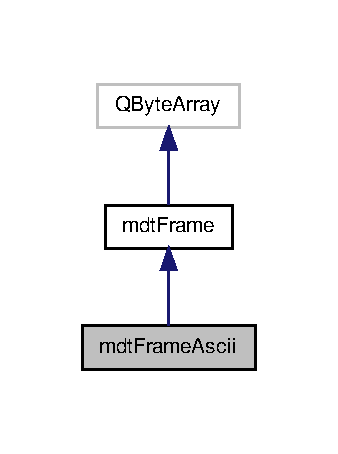
\includegraphics[width=162pt]{classmdt_frame_ascii__inherit__graph}
\end{center}
\end{figure}


Collaboration diagram for mdtFrameAscii:\nopagebreak
\begin{figure}[H]
\begin{center}
\leavevmode
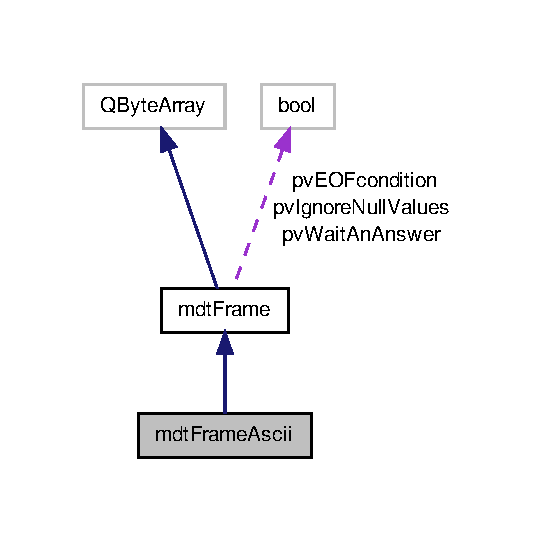
\includegraphics[width=162pt]{classmdt_frame_ascii__coll__graph}
\end{center}
\end{figure}
\subsection*{Public Member Functions}
\begin{DoxyCompactItemize}
\item 
\hypertarget{classmdt_frame_ascii_a64509246c1fd81ae79009a1ef9e4149b}{
void \hyperlink{classmdt_frame_ascii_a64509246c1fd81ae79009a1ef9e4149b}{setEofSeq} (const QByteArray \&eof)}
\label{classmdt_frame_ascii_a64509246c1fd81ae79009a1ef9e4149b}

\begin{DoxyCompactList}\small\item\em Set the end of frame sequence Note: if eof is empty, the null char ('$\backslash$0') is considered. \end{DoxyCompactList}\item 
\hypertarget{classmdt_frame_ascii_a9694c60a807fd2e80e293a66c193baaa}{
int \hyperlink{classmdt_frame_ascii_a9694c60a807fd2e80e293a66c193baaa}{eofSeqLen} ()}
\label{classmdt_frame_ascii_a9694c60a807fd2e80e293a66c193baaa}

\begin{DoxyCompactList}\small\item\em Get the length of the end of frame sequence. \end{DoxyCompactList}\item 
int \hyperlink{classmdt_frame_ascii_a9ef48ef78d9603a9d8c3be7e39b03745}{putData} (const char $\ast$data, int maxLen)
\begin{DoxyCompactList}\small\item\em Put data into the frame. \end{DoxyCompactList}\end{DoxyCompactItemize}


\subsection{Member Function Documentation}
\hypertarget{classmdt_frame_ascii_a9ef48ef78d9603a9d8c3be7e39b03745}{
\index{mdtFrameAscii@{mdtFrameAscii}!putData@{putData}}
\index{putData@{putData}!mdtFrameAscii@{mdtFrameAscii}}
\subsubsection[{putData}]{\setlength{\rightskip}{0pt plus 5cm}int mdtFrameAscii::putData (
\begin{DoxyParamCaption}
\item[{const char $\ast$}]{data, }
\item[{int}]{len}
\end{DoxyParamCaption}
)\hspace{0.3cm}{\ttfamily  \mbox{[}virtual\mbox{]}}}}
\label{classmdt_frame_ascii_a9ef48ef78d9603a9d8c3be7e39b03745}


Put data into the frame. 

Must be implemented by specific frame subclass. This method is called by the RX thread. Default implementation simply stores the maximum data as possible. No flags ares set. 
\begin{DoxyParams}{Parameters}
{\em data} & Valid pointer to the data \\
\hline
{\em len} & Maximum number of byte to store, must not be more than data size \\
\hline
\end{DoxyParams}
\begin{DoxyReturn}{Returns}
Number of bytes that could really be stored 
\end{DoxyReturn}
\begin{DoxyPrecond}{Precondition}
The data pointer must be valid, and not be the internal pointer returned by data(). 
\end{DoxyPrecond}


Reimplemented from \hyperlink{classmdt_frame_ae63af784d2fc54430ea5db4dc80b7ec8}{mdtFrame}.



The documentation for this class was generated from the following files:\begin{DoxyCompactItemize}
\item 
src/mdtutils/mdtFrameAscii.h\item 
src/mdtutils/mdtFrameAscii.cpp\end{DoxyCompactItemize}

\hypertarget{classmdt_frame_codec}{
\section{mdtFrameCodec Class Reference}
\label{classmdt_frame_codec}\index{mdtFrameCodec@{mdtFrameCodec}}
}


Inheritance diagram for mdtFrameCodec:\nopagebreak
\begin{figure}[H]
\begin{center}
\leavevmode
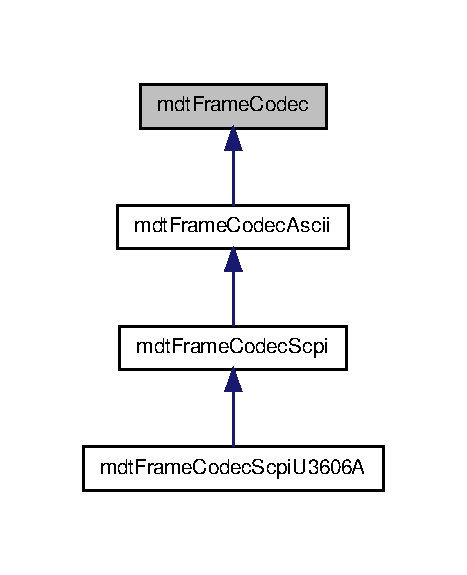
\includegraphics[width=224pt]{classmdt_frame_codec__inherit__graph}
\end{center}
\end{figure}
\subsection*{Protected Member Functions}
\begin{DoxyCompactItemize}
\item 
\hypertarget{classmdt_frame_codec_a6a47e1739b13c72883a01f5dd4bcffb6}{
bool {\bfseries decodeIEEEdata} (QByteArray data)}
\label{classmdt_frame_codec_a6a47e1739b13c72883a01f5dd4bcffb6}

\end{DoxyCompactItemize}
\subsection*{Protected Attributes}
\begin{DoxyCompactItemize}
\item 
\hypertarget{classmdt_frame_codec_a3e7dc48b11dda3688f48eea2030f0953}{
QList$<$ QVariant $>$ {\bfseries pvValues}}
\label{classmdt_frame_codec_a3e7dc48b11dda3688f48eea2030f0953}

\end{DoxyCompactItemize}


The documentation for this class was generated from the following files:\begin{DoxyCompactItemize}
\item 
src/mdtutils/mdtFrameCodec.h\item 
src/mdtutils/mdtFrameCodec.cpp\end{DoxyCompactItemize}

\hypertarget{classmdt_frame_codec_ascii}{
\section{mdtFrameCodecAscii Class Reference}
\label{classmdt_frame_codec_ascii}\index{mdtFrameCodecAscii@{mdtFrameCodecAscii}}
}


Inheritance diagram for mdtFrameCodecAscii:
\nopagebreak
\begin{figure}[H]
\begin{center}
\leavevmode
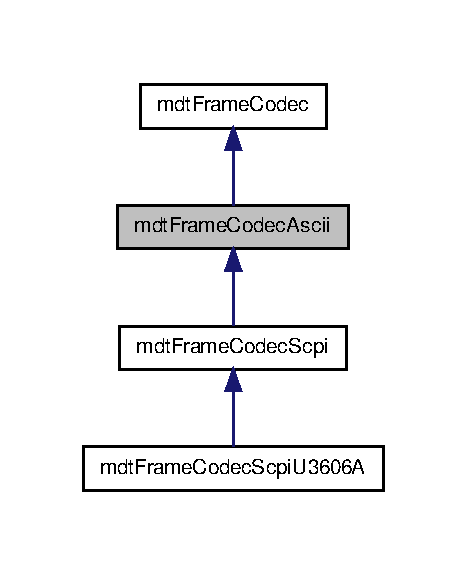
\includegraphics[width=224pt]{classmdt_frame_codec_ascii__inherit__graph}
\end{center}
\end{figure}


Collaboration diagram for mdtFrameCodecAscii:\nopagebreak
\begin{figure}[H]
\begin{center}
\leavevmode
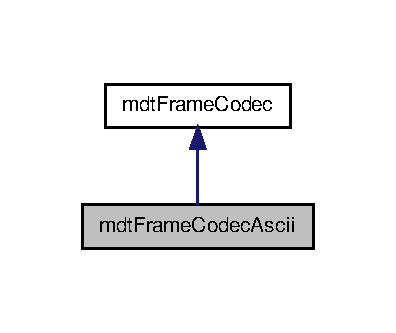
\includegraphics[width=190pt]{classmdt_frame_codec_ascii__coll__graph}
\end{center}
\end{figure}
\subsection*{Public Member Functions}
\begin{DoxyCompactItemize}
\item 
void \hyperlink{classmdt_frame_codec_ascii_a771d983498fb298595afbb97ee7a40f1}{setEofSeq} (QByteArray \&eofSeq)
\begin{DoxyCompactList}\small\item\em Set the Eond Of Frame Sequence. \end{DoxyCompactList}\item 
\hypertarget{classmdt_frame_codec_ascii_a0e8b9664e1451400e1b955c5180c0de8}{
void \hyperlink{classmdt_frame_codec_ascii_a0e8b9664e1451400e1b955c5180c0de8}{trim} ()}
\label{classmdt_frame_codec_ascii_a0e8b9664e1451400e1b955c5180c0de8}

\begin{DoxyCompactList}\small\item\em Remove whitespaces at begin and end of data frame. \end{DoxyCompactList}\item 
\hypertarget{classmdt_frame_codec_ascii_a119506d484a807d3486d47738ee22920}{
void \hyperlink{classmdt_frame_codec_ascii_a119506d484a807d3486d47738ee22920}{setCaseUpper} ()}
\label{classmdt_frame_codec_ascii_a119506d484a807d3486d47738ee22920}

\begin{DoxyCompactList}\small\item\em Set frame's data to upper case. \end{DoxyCompactList}\item 
\hypertarget{classmdt_frame_codec_ascii_aca3ccdf0bc617747e99ed1672344b880}{
QVariant \hyperlink{classmdt_frame_codec_ascii_aca3ccdf0bc617747e99ed1672344b880}{convertData} (const QString \&data) const }
\label{classmdt_frame_codec_ascii_aca3ccdf0bc617747e99ed1672344b880}

\begin{DoxyCompactList}\small\item\em Convert a string to first matching type. \end{DoxyCompactList}\end{DoxyCompactItemize}
\subsection*{Protected Member Functions}
\begin{DoxyCompactItemize}
\item 
bool \hyperlink{classmdt_frame_codec_ascii_a1dc1b7eda5e034c41b27c431227881e1}{clean} ()
\begin{DoxyCompactList}\small\item\em Clean frame. \end{DoxyCompactList}\item 
bool \hyperlink{classmdt_frame_codec_ascii_ab9aebbbadb6d40b1353634154e6a28c0}{removeEofSeq} ()
\begin{DoxyCompactList}\small\item\em Remove the End Of Frame Sequence. \end{DoxyCompactList}\end{DoxyCompactItemize}
\subsection*{Protected Attributes}
\begin{DoxyCompactItemize}
\item 
\hypertarget{classmdt_frame_codec_ascii_a1f912b05801a0db32c9fca0f2450bdb1}{
QString {\bfseries pvAsciiData}}
\label{classmdt_frame_codec_ascii_a1f912b05801a0db32c9fca0f2450bdb1}

\item 
\hypertarget{classmdt_frame_codec_ascii_ad44132c4e3db292c71831111da748c7a}{
QByteArray {\bfseries pvEofSeq}}
\label{classmdt_frame_codec_ascii_ad44132c4e3db292c71831111da748c7a}

\item 
\hypertarget{classmdt_frame_codec_ascii_aa47c85e69bc7609e21efe89de0b8308d}{
QStringList {\bfseries pvNodes}}
\label{classmdt_frame_codec_ascii_aa47c85e69bc7609e21efe89de0b8308d}

\end{DoxyCompactItemize}


\subsection{Detailed Description}


Definition at line 29 of file mdtFrameCodecAscii.h.



\subsection{Member Function Documentation}
\hypertarget{classmdt_frame_codec_ascii_a1dc1b7eda5e034c41b27c431227881e1}{
\index{mdtFrameCodecAscii@{mdtFrameCodecAscii}!clean@{clean}}
\index{clean@{clean}!mdtFrameCodecAscii@{mdtFrameCodecAscii}}
\subsubsection[{clean}]{\setlength{\rightskip}{0pt plus 5cm}bool mdtFrameCodecAscii::clean (
\begin{DoxyParamCaption}
{}
\end{DoxyParamCaption}
)\hspace{0.3cm}{\ttfamily  \mbox{[}protected\mbox{]}}}}
\label{classmdt_frame_codec_ascii_a1dc1b7eda5e034c41b27c431227881e1}


Clean frame. 

Helper method that removes white spaces at beginning and end of internal data (see QString::trimmed() ). Next, the EOF seuqence is removed.

If a step fails, a message is added to \hyperlink{classmdt_error}{mdtError} system.

\begin{DoxyReturn}{Returns}
true if EOF could be removed, and data size is $>$ 0 after clean. 
\end{DoxyReturn}


Definition at line 92 of file mdtFrameCodecAscii.cpp.

\hypertarget{classmdt_frame_codec_ascii_ab9aebbbadb6d40b1353634154e6a28c0}{
\index{mdtFrameCodecAscii@{mdtFrameCodecAscii}!removeEofSeq@{removeEofSeq}}
\index{removeEofSeq@{removeEofSeq}!mdtFrameCodecAscii@{mdtFrameCodecAscii}}
\subsubsection[{removeEofSeq}]{\setlength{\rightskip}{0pt plus 5cm}bool mdtFrameCodecAscii::removeEofSeq (
\begin{DoxyParamCaption}
{}
\end{DoxyParamCaption}
)\hspace{0.3cm}{\ttfamily  \mbox{[}protected\mbox{]}}}}
\label{classmdt_frame_codec_ascii_ab9aebbbadb6d40b1353634154e6a28c0}


Remove the End Of Frame Sequence. 

Note: this method does nothing if EofSeq was not set 

Definition at line 111 of file mdtFrameCodecAscii.cpp.

\hypertarget{classmdt_frame_codec_ascii_a771d983498fb298595afbb97ee7a40f1}{
\index{mdtFrameCodecAscii@{mdtFrameCodecAscii}!setEofSeq@{setEofSeq}}
\index{setEofSeq@{setEofSeq}!mdtFrameCodecAscii@{mdtFrameCodecAscii}}
\subsubsection[{setEofSeq}]{\setlength{\rightskip}{0pt plus 5cm}void mdtFrameCodecAscii::setEofSeq (
\begin{DoxyParamCaption}
\item[{QByteArray \&}]{eofSeq}
\end{DoxyParamCaption}
)}}
\label{classmdt_frame_codec_ascii_a771d983498fb298595afbb97ee7a40f1}


Set the Eond Of Frame Sequence. 

When using mdtLibrary's communication classes, the endOfFrame sequence is allready removed. So, this setup is optional. \begin{DoxySeeAlso}{See also}
\hyperlink{classmdt_frame}{mdtFrame} 

\hyperlink{classmdt_port}{mdtPort} 

\hyperlink{classmdt_port_manager}{mdtPortManager} 
\end{DoxySeeAlso}


Definition at line 34 of file mdtFrameCodecAscii.cpp.



The documentation for this class was generated from the following files:\begin{DoxyCompactItemize}
\item 
src/mdtutils/mdtFrameCodecAscii.h\item 
src/mdtutils/mdtFrameCodecAscii.cpp\end{DoxyCompactItemize}

\hypertarget{classmdt_frame_codec_modbus}{
\section{mdtFrameCodecModbus Class Reference}
\label{classmdt_frame_codec_modbus}\index{mdtFrameCodecModbus@{mdtFrameCodecModbus}}
}


Encode and decode MODBUS PDU NOTE: stockage des adresses durant Q/R ?  




{\ttfamily \#include $<$mdtFrameCodecModbus.h$>$}



Inheritance diagram for mdtFrameCodecModbus:\nopagebreak
\begin{figure}[H]
\begin{center}
\leavevmode
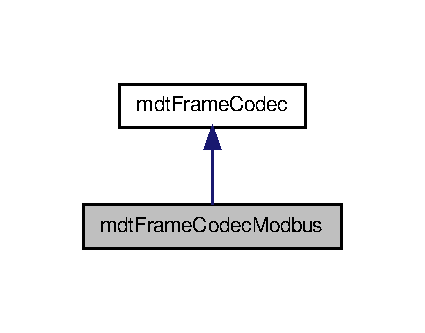
\includegraphics[width=204pt]{classmdt_frame_codec_modbus__inherit__graph}
\end{center}
\end{figure}


Collaboration diagram for mdtFrameCodecModbus:\nopagebreak
\begin{figure}[H]
\begin{center}
\leavevmode
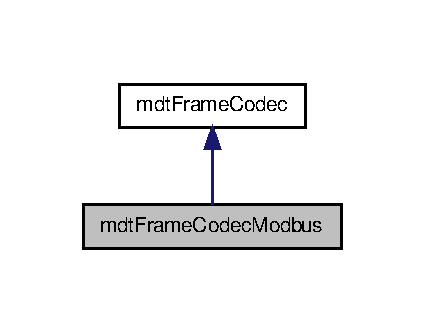
\includegraphics[width=204pt]{classmdt_frame_codec_modbus__coll__graph}
\end{center}
\end{figure}
\subsection*{Public Types}
\begin{DoxyCompactItemize}
\item 
enum \hyperlink{classmdt_frame_codec_modbus_a31d8291be7f8636d5d295ce3066d7ac7}{modbus\_\-error\_\-code\_\-t} \{ \par
\hyperlink{classmdt_frame_codec_modbus_a31d8291be7f8636d5d295ce3066d7ac7aab1a954c9125bbf1f79c69d480faec4b}{UNKNOW\_\-ERROR}, 
\hyperlink{classmdt_frame_codec_modbus_a31d8291be7f8636d5d295ce3066d7ac7aab0437de7413a72446c491f518249a0a}{ILLEGAL\_\-FUNCTION} =  1, 
\hyperlink{classmdt_frame_codec_modbus_a31d8291be7f8636d5d295ce3066d7ac7a1eeaee68c0cb3fc2c9dd26e9540c4fc3}{ILLEGAL\_\-DATA\_\-ADDRESS}, 
\hyperlink{classmdt_frame_codec_modbus_a31d8291be7f8636d5d295ce3066d7ac7a99ff0045d822da03e709508ce1acf85b}{ILLEGAL\_\-DATA\_\-VALUE}, 
\par
\hyperlink{classmdt_frame_codec_modbus_a31d8291be7f8636d5d295ce3066d7ac7aa458eaabf779b5936891a69d64eb05ac}{SLAVE\_\-DEVICE\_\-FAILURE}, 
\hyperlink{classmdt_frame_codec_modbus_a31d8291be7f8636d5d295ce3066d7ac7abcc3d663faf228569aea757d3c26611d}{ACKNOWLEDGE}, 
\hyperlink{classmdt_frame_codec_modbus_a31d8291be7f8636d5d295ce3066d7ac7afc6561ef2b014e3dd0e6ae2dd1d09201}{SLAVE\_\-DEVICE\_\-BUSY}, 
\hyperlink{classmdt_frame_codec_modbus_a31d8291be7f8636d5d295ce3066d7ac7ade44de70235367650161630c7dde3c4b}{RESERVE\_\-ERROR\_\-7}, 
\par
\hyperlink{classmdt_frame_codec_modbus_a31d8291be7f8636d5d295ce3066d7ac7a82a7c52e774764f6b76d286bde96accf}{MEMORY\_\-PARITY\_\-ERROR}, 
\hyperlink{classmdt_frame_codec_modbus_a31d8291be7f8636d5d295ce3066d7ac7a956e96d465ca9152e77d09ee022b1a5f}{RESERVE\_\-ERROR\_\-9}, 
\hyperlink{classmdt_frame_codec_modbus_a31d8291be7f8636d5d295ce3066d7ac7a8a4a5e81091eb2c57fd57dee450a2770}{GATEWAY\_\-PATH\_\-UNAVAILABLE}, 
\hyperlink{classmdt_frame_codec_modbus_a31d8291be7f8636d5d295ce3066d7ac7a9ca48eb9d1ab05850c36170e7dac0b99}{GATEWAY\_\-TARGET\_\-RESPONSE}
 \}
\begin{DoxyCompactList}\small\item\em MODBUS response error code. \end{DoxyCompactList}\end{DoxyCompactItemize}
\subsection*{Public Member Functions}
\begin{DoxyCompactItemize}
\item 
QByteArray \hyperlink{classmdt_frame_codec_modbus_adf0a4d583aeff7b818dda94514c594f0}{encodeReadCoils} (quint16 startAddress, quint16 n)
\begin{DoxyCompactList}\small\item\em Encode a PDU according the ReadCoils function (0x01) \end{DoxyCompactList}\item 
QByteArray \hyperlink{classmdt_frame_codec_modbus_a123f63422bb34fcb10ac653c0e89e79e}{encodeWriteSingleCoil} (quint16 address, bool state)
\begin{DoxyCompactList}\small\item\em Encode a PDU according the WriteSingleCoil function (0x05) \end{DoxyCompactList}\item 
int \hyperlink{classmdt_frame_codec_modbus_a426f465363a49d70890a462b40677787}{decode} (const QByteArray \&pdu)
\begin{DoxyCompactList}\small\item\em Decode a MODBUS PDU. \end{DoxyCompactList}\item 
\hyperlink{classmdt_frame_codec_modbus_a31d8291be7f8636d5d295ce3066d7ac7}{modbus\_\-error\_\-code\_\-t} \hyperlink{classmdt_frame_codec_modbus_a21f3102e12f1a1d9c4145c1ce1f8e6b6}{lastModbusError} ()
\begin{DoxyCompactList}\small\item\em Get the last MODBUS error code returned. \end{DoxyCompactList}\end{DoxyCompactItemize}


\subsection{Detailed Description}
Encode and decode MODBUS PDU NOTE: stockage des adresses durant Q/R ? 

This class works only on MODBUS PDU. To transmit MODBUS/TCP frame, the resulting PDU can be sent using \hyperlink{classmdt_frame_modbus_tcp}{mdtFrameModbusTcp} class, or received PDU decoded here.

References:
\begin{DoxyItemize}
\item MODBUS Application Protocol Specification V1.1b
\item \href{http://www.Modbus-IDA.org}{\tt http://www.Modbus-\/IDA.org}
\end{DoxyItemize}

\begin{DoxySeeAlso}{See also}
\hyperlink{classmdt_frame_codec}{mdtFrameCodec} 

\hyperlink{classmdt_frame_modbus_tcp}{mdtFrameModbusTcp} 
\end{DoxySeeAlso}


Definition at line 41 of file mdtFrameCodecModbus.h.



\subsection{Member Enumeration Documentation}
\hypertarget{classmdt_frame_codec_modbus_a31d8291be7f8636d5d295ce3066d7ac7}{
\index{mdtFrameCodecModbus@{mdtFrameCodecModbus}!modbus\_\-error\_\-code\_\-t@{modbus\_\-error\_\-code\_\-t}}
\index{modbus\_\-error\_\-code\_\-t@{modbus\_\-error\_\-code\_\-t}!mdtFrameCodecModbus@{mdtFrameCodecModbus}}
\subsubsection[{modbus\_\-error\_\-code\_\-t}]{\setlength{\rightskip}{0pt plus 5cm}enum {\bf mdtFrameCodecModbus::modbus\_\-error\_\-code\_\-t}}}
\label{classmdt_frame_codec_modbus_a31d8291be7f8636d5d295ce3066d7ac7}


MODBUS response error code. 

\begin{Desc}
\item[Enumerator: ]\par
\begin{description}
\index{UNKNOW\_\-ERROR@{UNKNOW\_\-ERROR}!mdtFrameCodecModbus@{mdtFrameCodecModbus}}\index{mdtFrameCodecModbus@{mdtFrameCodecModbus}!UNKNOW\_\-ERROR@{UNKNOW\_\-ERROR}}\item[{\em 
\hypertarget{classmdt_frame_codec_modbus_a31d8291be7f8636d5d295ce3066d7ac7aab1a954c9125bbf1f79c69d480faec4b}{
UNKNOW\_\-ERROR}
\label{classmdt_frame_codec_modbus_a31d8291be7f8636d5d295ce3066d7ac7aab1a954c9125bbf1f79c69d480faec4b}
}]Error is unknow from codec \index{ILLEGAL\_\-FUNCTION@{ILLEGAL\_\-FUNCTION}!mdtFrameCodecModbus@{mdtFrameCodecModbus}}\index{mdtFrameCodecModbus@{mdtFrameCodecModbus}!ILLEGAL\_\-FUNCTION@{ILLEGAL\_\-FUNCTION}}\item[{\em 
\hypertarget{classmdt_frame_codec_modbus_a31d8291be7f8636d5d295ce3066d7ac7aab0437de7413a72446c491f518249a0a}{
ILLEGAL\_\-FUNCTION}
\label{classmdt_frame_codec_modbus_a31d8291be7f8636d5d295ce3066d7ac7aab0437de7413a72446c491f518249a0a}
}]Code 0x01: Function is not allowed for the server \index{ILLEGAL\_\-DATA\_\-ADDRESS@{ILLEGAL\_\-DATA\_\-ADDRESS}!mdtFrameCodecModbus@{mdtFrameCodecModbus}}\index{mdtFrameCodecModbus@{mdtFrameCodecModbus}!ILLEGAL\_\-DATA\_\-ADDRESS@{ILLEGAL\_\-DATA\_\-ADDRESS}}\item[{\em 
\hypertarget{classmdt_frame_codec_modbus_a31d8291be7f8636d5d295ce3066d7ac7a1eeaee68c0cb3fc2c9dd26e9540c4fc3}{
ILLEGAL\_\-DATA\_\-ADDRESS}
\label{classmdt_frame_codec_modbus_a31d8291be7f8636d5d295ce3066d7ac7a1eeaee68c0cb3fc2c9dd26e9540c4fc3}
}]Code 0x02: Request address is not in range of the server \index{ILLEGAL\_\-DATA\_\-VALUE@{ILLEGAL\_\-DATA\_\-VALUE}!mdtFrameCodecModbus@{mdtFrameCodecModbus}}\index{mdtFrameCodecModbus@{mdtFrameCodecModbus}!ILLEGAL\_\-DATA\_\-VALUE@{ILLEGAL\_\-DATA\_\-VALUE}}\item[{\em 
\hypertarget{classmdt_frame_codec_modbus_a31d8291be7f8636d5d295ce3066d7ac7a99ff0045d822da03e709508ce1acf85b}{
ILLEGAL\_\-DATA\_\-VALUE}
\label{classmdt_frame_codec_modbus_a31d8291be7f8636d5d295ce3066d7ac7a99ff0045d822da03e709508ce1acf85b}
}]Code 0x03: Request value is not in allowed from server \index{SLAVE\_\-DEVICE\_\-FAILURE@{SLAVE\_\-DEVICE\_\-FAILURE}!mdtFrameCodecModbus@{mdtFrameCodecModbus}}\index{mdtFrameCodecModbus@{mdtFrameCodecModbus}!SLAVE\_\-DEVICE\_\-FAILURE@{SLAVE\_\-DEVICE\_\-FAILURE}}\item[{\em 
\hypertarget{classmdt_frame_codec_modbus_a31d8291be7f8636d5d295ce3066d7ac7aa458eaabf779b5936891a69d64eb05ac}{
SLAVE\_\-DEVICE\_\-FAILURE}
\label{classmdt_frame_codec_modbus_a31d8291be7f8636d5d295ce3066d7ac7aa458eaabf779b5936891a69d64eb05ac}
}]Code 0x04: Unrecoverable failue on server \index{ACKNOWLEDGE@{ACKNOWLEDGE}!mdtFrameCodecModbus@{mdtFrameCodecModbus}}\index{mdtFrameCodecModbus@{mdtFrameCodecModbus}!ACKNOWLEDGE@{ACKNOWLEDGE}}\item[{\em 
\hypertarget{classmdt_frame_codec_modbus_a31d8291be7f8636d5d295ce3066d7ac7abcc3d663faf228569aea757d3c26611d}{
ACKNOWLEDGE}
\label{classmdt_frame_codec_modbus_a31d8291be7f8636d5d295ce3066d7ac7abcc3d663faf228569aea757d3c26611d}
}]Code 0x05: Request accepted, but mor time is needed (server side) for response \index{SLAVE\_\-DEVICE\_\-BUSY@{SLAVE\_\-DEVICE\_\-BUSY}!mdtFrameCodecModbus@{mdtFrameCodecModbus}}\index{mdtFrameCodecModbus@{mdtFrameCodecModbus}!SLAVE\_\-DEVICE\_\-BUSY@{SLAVE\_\-DEVICE\_\-BUSY}}\item[{\em 
\hypertarget{classmdt_frame_codec_modbus_a31d8291be7f8636d5d295ce3066d7ac7afc6561ef2b014e3dd0e6ae2dd1d09201}{
SLAVE\_\-DEVICE\_\-BUSY}
\label{classmdt_frame_codec_modbus_a31d8291be7f8636d5d295ce3066d7ac7afc6561ef2b014e3dd0e6ae2dd1d09201}
}]Code 0x06: Server busy, client should try to resend the query later \index{RESERVE\_\-ERROR\_\-7@{RESERVE\_\-ERROR\_\-7}!mdtFrameCodecModbus@{mdtFrameCodecModbus}}\index{mdtFrameCodecModbus@{mdtFrameCodecModbus}!RESERVE\_\-ERROR\_\-7@{RESERVE\_\-ERROR\_\-7}}\item[{\em 
\hypertarget{classmdt_frame_codec_modbus_a31d8291be7f8636d5d295ce3066d7ac7ade44de70235367650161630c7dde3c4b}{
RESERVE\_\-ERROR\_\-7}
\label{classmdt_frame_codec_modbus_a31d8291be7f8636d5d295ce3066d7ac7ade44de70235367650161630c7dde3c4b}
}]Not used in current specification \index{MEMORY\_\-PARITY\_\-ERROR@{MEMORY\_\-PARITY\_\-ERROR}!mdtFrameCodecModbus@{mdtFrameCodecModbus}}\index{mdtFrameCodecModbus@{mdtFrameCodecModbus}!MEMORY\_\-PARITY\_\-ERROR@{MEMORY\_\-PARITY\_\-ERROR}}\item[{\em 
\hypertarget{classmdt_frame_codec_modbus_a31d8291be7f8636d5d295ce3066d7ac7a82a7c52e774764f6b76d286bde96accf}{
MEMORY\_\-PARITY\_\-ERROR}
\label{classmdt_frame_codec_modbus_a31d8291be7f8636d5d295ce3066d7ac7a82a7c52e774764f6b76d286bde96accf}
}]Code 0x08: Parity error related to code function 20 and 21 \index{RESERVE\_\-ERROR\_\-9@{RESERVE\_\-ERROR\_\-9}!mdtFrameCodecModbus@{mdtFrameCodecModbus}}\index{mdtFrameCodecModbus@{mdtFrameCodecModbus}!RESERVE\_\-ERROR\_\-9@{RESERVE\_\-ERROR\_\-9}}\item[{\em 
\hypertarget{classmdt_frame_codec_modbus_a31d8291be7f8636d5d295ce3066d7ac7a956e96d465ca9152e77d09ee022b1a5f}{
RESERVE\_\-ERROR\_\-9}
\label{classmdt_frame_codec_modbus_a31d8291be7f8636d5d295ce3066d7ac7a956e96d465ca9152e77d09ee022b1a5f}
}]Not used in current specification \index{GATEWAY\_\-PATH\_\-UNAVAILABLE@{GATEWAY\_\-PATH\_\-UNAVAILABLE}!mdtFrameCodecModbus@{mdtFrameCodecModbus}}\index{mdtFrameCodecModbus@{mdtFrameCodecModbus}!GATEWAY\_\-PATH\_\-UNAVAILABLE@{GATEWAY\_\-PATH\_\-UNAVAILABLE}}\item[{\em 
\hypertarget{classmdt_frame_codec_modbus_a31d8291be7f8636d5d295ce3066d7ac7a8a4a5e81091eb2c57fd57dee450a2770}{
GATEWAY\_\-PATH\_\-UNAVAILABLE}
\label{classmdt_frame_codec_modbus_a31d8291be7f8636d5d295ce3066d7ac7a8a4a5e81091eb2c57fd57dee450a2770}
}]Code 0x0A: Error from a gateway (misconfigured or overloaded) \index{GATEWAY\_\-TARGET\_\-RESPONSE@{GATEWAY\_\-TARGET\_\-RESPONSE}!mdtFrameCodecModbus@{mdtFrameCodecModbus}}\index{mdtFrameCodecModbus@{mdtFrameCodecModbus}!GATEWAY\_\-TARGET\_\-RESPONSE@{GATEWAY\_\-TARGET\_\-RESPONSE}}\item[{\em 
\hypertarget{classmdt_frame_codec_modbus_a31d8291be7f8636d5d295ce3066d7ac7a9ca48eb9d1ab05850c36170e7dac0b99}{
GATEWAY\_\-TARGET\_\-RESPONSE}
\label{classmdt_frame_codec_modbus_a31d8291be7f8636d5d295ce3066d7ac7a9ca48eb9d1ab05850c36170e7dac0b99}
}]Code 0x0B: Error from a gateway: target device not present on network \end{description}
\end{Desc}



Definition at line 47 of file mdtFrameCodecModbus.h.



\subsection{Member Function Documentation}
\hypertarget{classmdt_frame_codec_modbus_a426f465363a49d70890a462b40677787}{
\index{mdtFrameCodecModbus@{mdtFrameCodecModbus}!decode@{decode}}
\index{decode@{decode}!mdtFrameCodecModbus@{mdtFrameCodecModbus}}
\subsubsection[{decode}]{\setlength{\rightskip}{0pt plus 5cm}int mdtFrameCodecModbus::decode (
\begin{DoxyParamCaption}
\item[{const QByteArray \&}]{pdu}
\end{DoxyParamCaption}
)}}
\label{classmdt_frame_codec_modbus_a426f465363a49d70890a462b40677787}


Decode a MODBUS PDU. 

This should reconize the function code in PDU, and call the appropriate decode methode (internall). Once decode is done, the values are available with \hyperlink{classmdt_frame_codec_a599a46e2d7cb5f80bd80e303236ead73}{mdtFrameCodec::values()}. To know what was decoded, the function code is returned.\par
 The values are stored in a QList$<$QVariant$>$ , with format depending of the function code:
\begin{DoxyItemize}
\item For a ReadCoils response, values will be bool, sorted by ascending addresses.
\end{DoxyItemize}

If PDU contains a error code, the list of values will be empty, and this error code will be returned.\par
 If a MODBUS error code is decoded, this error code is returned as in frame (for. ex: 0x81 for a ReadCoils error) To know whitch MODBUS error was returned, use \hyperlink{classmdt_frame_codec_modbus_a21f3102e12f1a1d9c4145c1ce1f8e6b6}{lastModbusError()}


\begin{DoxyParams}{Parameters}
{\em pdu} & The MODBUS PDU to decode \\
\hline
\end{DoxyParams}
\begin{DoxyReturn}{Returns}
Decoded function code, MODBUS error code or value $<$ 0 on other error. 
\end{DoxyReturn}


NOTE:\begin{Desc}
\item[\hyperlink{todo__todo000041}{Todo}]Base 16 ?? \end{Desc}




Definition at line 80 of file mdtFrameCodecModbus.cpp.

\hypertarget{classmdt_frame_codec_modbus_adf0a4d583aeff7b818dda94514c594f0}{
\index{mdtFrameCodecModbus@{mdtFrameCodecModbus}!encodeReadCoils@{encodeReadCoils}}
\index{encodeReadCoils@{encodeReadCoils}!mdtFrameCodecModbus@{mdtFrameCodecModbus}}
\subsubsection[{encodeReadCoils}]{\setlength{\rightskip}{0pt plus 5cm}QByteArray mdtFrameCodecModbus::encodeReadCoils (
\begin{DoxyParamCaption}
\item[{quint16}]{startAddress, }
\item[{quint16}]{n}
\end{DoxyParamCaption}
)}}
\label{classmdt_frame_codec_modbus_adf0a4d583aeff7b818dda94514c594f0}


Encode a PDU according the ReadCoils function (0x01) 

Please take a look at MODBUS specifications for more details. \begin{DoxyReturn}{Returns}
A QByteArray containing the PDU, or a empty QByteArray on error. 
\end{DoxyReturn}


Definition at line 36 of file mdtFrameCodecModbus.cpp.

\hypertarget{classmdt_frame_codec_modbus_a123f63422bb34fcb10ac653c0e89e79e}{
\index{mdtFrameCodecModbus@{mdtFrameCodecModbus}!encodeWriteSingleCoil@{encodeWriteSingleCoil}}
\index{encodeWriteSingleCoil@{encodeWriteSingleCoil}!mdtFrameCodecModbus@{mdtFrameCodecModbus}}
\subsubsection[{encodeWriteSingleCoil}]{\setlength{\rightskip}{0pt plus 5cm}QByteArray mdtFrameCodecModbus::encodeWriteSingleCoil (
\begin{DoxyParamCaption}
\item[{quint16}]{address, }
\item[{bool}]{state}
\end{DoxyParamCaption}
)}}
\label{classmdt_frame_codec_modbus_a123f63422bb34fcb10ac653c0e89e79e}


Encode a PDU according the WriteSingleCoil function (0x05) 

Please take a look at MODBUS specifications for more details. \begin{DoxyReturn}{Returns}
A QByteArray containing the PDU, or a empty QByteArray on error. 
\end{DoxyReturn}


Definition at line 60 of file mdtFrameCodecModbus.cpp.

\hypertarget{classmdt_frame_codec_modbus_a21f3102e12f1a1d9c4145c1ce1f8e6b6}{
\index{mdtFrameCodecModbus@{mdtFrameCodecModbus}!lastModbusError@{lastModbusError}}
\index{lastModbusError@{lastModbusError}!mdtFrameCodecModbus@{mdtFrameCodecModbus}}
\subsubsection[{lastModbusError}]{\setlength{\rightskip}{0pt plus 5cm}{\bf mdtFrameCodecModbus::modbus\_\-error\_\-code\_\-t} mdtFrameCodecModbus::lastModbusError (
\begin{DoxyParamCaption}
{}
\end{DoxyParamCaption}
)}}
\label{classmdt_frame_codec_modbus_a21f3102e12f1a1d9c4145c1ce1f8e6b6}


Get the last MODBUS error code returned. 

Returns the error code according to the specification, part function/error codes (same value). \begin{DoxySeeAlso}{See also}
\hyperlink{classmdt_frame_codec_modbus_a426f465363a49d70890a462b40677787}{decode()} 
\end{DoxySeeAlso}


Definition at line 131 of file mdtFrameCodecModbus.cpp.



The documentation for this class was generated from the following files:\begin{DoxyCompactItemize}
\item 
src/mdtutils/mdtFrameCodecModbus.h\item 
src/mdtutils/mdtFrameCodecModbus.cpp\end{DoxyCompactItemize}

\hypertarget{classmdt_frame_codec_scpi}{
\section{mdtFrameCodecScpi Class Reference}
\label{classmdt_frame_codec_scpi}\index{mdtFrameCodecScpi@{mdtFrameCodecScpi}}
}


Decode SCPI data.  




{\ttfamily \#include $<$mdtFrameCodecScpi.h$>$}



Inheritance diagram for mdtFrameCodecScpi:\nopagebreak
\begin{figure}[H]
\begin{center}
\leavevmode
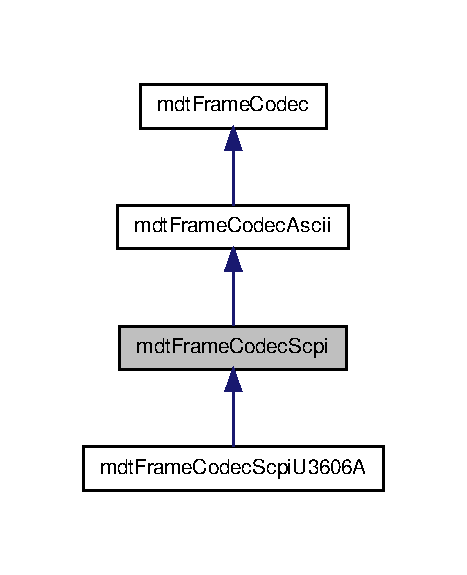
\includegraphics[width=224pt]{classmdt_frame_codec_scpi__inherit__graph}
\end{center}
\end{figure}


Collaboration diagram for mdtFrameCodecScpi:\nopagebreak
\begin{figure}[H]
\begin{center}
\leavevmode
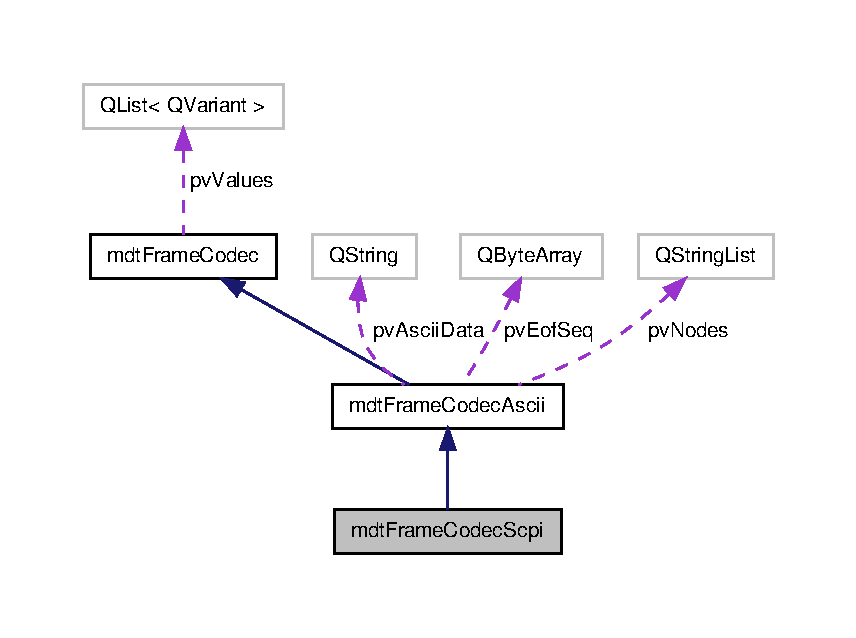
\includegraphics[width=190pt]{classmdt_frame_codec_scpi__coll__graph}
\end{center}
\end{figure}
\subsection*{Public Types}
\begin{DoxyCompactItemize}
\item 
enum \hyperlink{classmdt_frame_codec_scpi_a1aafb008a4207cc922f46fe905b3f17d}{waveform\_\-format} \{ \hyperlink{classmdt_frame_codec_scpi_a1aafb008a4207cc922f46fe905b3f17da7f4b47afe74504dea43bb04c8c6fbe58}{WORD}, 
\hyperlink{classmdt_frame_codec_scpi_a1aafb008a4207cc922f46fe905b3f17daad91226f87cea7fab38f5cc7618f424c}{BYTE}, 
\hyperlink{classmdt_frame_codec_scpi_a1aafb008a4207cc922f46fe905b3f17da957445cd510a5c4e6964e9b79e73af4d}{ASCII}
 \}
\begin{DoxyCompactList}\small\item\em Format of waveform data. \end{DoxyCompactList}\end{DoxyCompactItemize}
\subsection*{Public Member Functions}
\begin{DoxyCompactItemize}
\item 
bool \hyperlink{classmdt_frame_codec_scpi_a37a1703b6daee6f6bf91c6afb46191b3}{decodeValues} (const QByteArray \&data, QString sep=\char`\"{}:\char`\"{})
\begin{DoxyCompactList}\small\item\em Decode SCPI value(s) \end{DoxyCompactList}\item 
bool \hyperlink{classmdt_frame_codec_scpi_a6ddd1b8e23252dc7f03c279a030cb36f}{decodeIdn} (const QByteArray \&data)
\begin{DoxyCompactList}\small\item\em Decode the IDN answer. \end{DoxyCompactList}\item 
bool \hyperlink{classmdt_frame_codec_scpi_a9e38d8afadc7ff37821620feea6b0899}{decodeError} (const QByteArray \&data)
\begin{DoxyCompactList}\small\item\em Decode error answer. \end{DoxyCompactList}\item 
bool \hyperlink{classmdt_frame_codec_scpi_a0123b42b9e351b0ef3c13d34a5c4d45e}{decodeIEEEblock} (const QByteArray \&data, \hyperlink{classmdt_frame_codec_scpi_a1aafb008a4207cc922f46fe905b3f17d}{waveform\_\-format} format)
\begin{DoxyCompactList}\small\item\em Decode a IEEE block. \end{DoxyCompactList}\end{DoxyCompactItemize}
\subsection*{Protected Member Functions}
\begin{DoxyCompactItemize}
\item 
bool \hyperlink{classmdt_frame_codec_scpi_aa6596dc898438be704191ad282d02100}{decodeIEEEdataAscii} (const QByteArray \&data)
\begin{DoxyCompactList}\small\item\em Decode a array of ASCII values. \end{DoxyCompactList}\item 
bool \hyperlink{classmdt_frame_codec_scpi_ab70c6c3d2d91ddff065952b6c2db8345}{decodeIEEEdataByte} (const QByteArray \&data)
\begin{DoxyCompactList}\small\item\em Decode a array of BYTE values. \end{DoxyCompactList}\end{DoxyCompactItemize}


\subsection{Detailed Description}
Decode SCPI data. 

Definition at line 38 of file mdtFrameCodecScpi.h.



\subsection{Member Enumeration Documentation}
\hypertarget{classmdt_frame_codec_scpi_a1aafb008a4207cc922f46fe905b3f17d}{
\index{mdtFrameCodecScpi@{mdtFrameCodecScpi}!waveform\_\-format@{waveform\_\-format}}
\index{waveform\_\-format@{waveform\_\-format}!mdtFrameCodecScpi@{mdtFrameCodecScpi}}
\subsubsection[{waveform\_\-format}]{\setlength{\rightskip}{0pt plus 5cm}enum {\bf mdtFrameCodecScpi::waveform\_\-format}}}
\label{classmdt_frame_codec_scpi_a1aafb008a4207cc922f46fe905b3f17d}


Format of waveform data. 

\begin{Desc}
\item[Enumerator: ]\par
\begin{description}
\index{WORD@{WORD}!mdtFrameCodecScpi@{mdtFrameCodecScpi}}\index{mdtFrameCodecScpi@{mdtFrameCodecScpi}!WORD@{WORD}}\item[{\em 
\hypertarget{classmdt_frame_codec_scpi_a1aafb008a4207cc922f46fe905b3f17da7f4b47afe74504dea43bb04c8c6fbe58}{
WORD}
\label{classmdt_frame_codec_scpi_a1aafb008a4207cc922f46fe905b3f17da7f4b47afe74504dea43bb04c8c6fbe58}
}]16 bit data resolution \index{BYTE@{BYTE}!mdtFrameCodecScpi@{mdtFrameCodecScpi}}\index{mdtFrameCodecScpi@{mdtFrameCodecScpi}!BYTE@{BYTE}}\item[{\em 
\hypertarget{classmdt_frame_codec_scpi_a1aafb008a4207cc922f46fe905b3f17daad91226f87cea7fab38f5cc7618f424c}{
BYTE}
\label{classmdt_frame_codec_scpi_a1aafb008a4207cc922f46fe905b3f17daad91226f87cea7fab38f5cc7618f424c}
}]8 bit data resolution \index{ASCII@{ASCII}!mdtFrameCodecScpi@{mdtFrameCodecScpi}}\index{mdtFrameCodecScpi@{mdtFrameCodecScpi}!ASCII@{ASCII}}\item[{\em 
\hypertarget{classmdt_frame_codec_scpi_a1aafb008a4207cc922f46fe905b3f17da957445cd510a5c4e6964e9b79e73af4d}{
ASCII}
\label{classmdt_frame_codec_scpi_a1aafb008a4207cc922f46fe905b3f17da957445cd510a5c4e6964e9b79e73af4d}
}]ASCII float represented data \end{description}
\end{Desc}



Definition at line 44 of file mdtFrameCodecScpi.h.



\subsection{Member Function Documentation}
\hypertarget{classmdt_frame_codec_scpi_a9e38d8afadc7ff37821620feea6b0899}{
\index{mdtFrameCodecScpi@{mdtFrameCodecScpi}!decodeError@{decodeError}}
\index{decodeError@{decodeError}!mdtFrameCodecScpi@{mdtFrameCodecScpi}}
\subsubsection[{decodeError}]{\setlength{\rightskip}{0pt plus 5cm}bool mdtFrameCodecScpi::decodeError (
\begin{DoxyParamCaption}
\item[{const QByteArray \&}]{data}
\end{DoxyParamCaption}
)}}
\label{classmdt_frame_codec_scpi_a9e38d8afadc7ff37821620feea6b0899}


Decode error answer. 

When decode was done successfully, error is available with \hyperlink{classmdt_frame_codec_a2c0cc0f9d9b72ef2295b7ec7eca72ea7}{values()}:
\begin{DoxyItemize}
\item Item 0 is the error number
\item Item 1 is the error message string
\item After item 1 are device's specific messages (if exists) 
\end{DoxyItemize}

Definition at line 120 of file mdtFrameCodecScpi.cpp.

\hypertarget{classmdt_frame_codec_scpi_a6ddd1b8e23252dc7f03c279a030cb36f}{
\index{mdtFrameCodecScpi@{mdtFrameCodecScpi}!decodeIdn@{decodeIdn}}
\index{decodeIdn@{decodeIdn}!mdtFrameCodecScpi@{mdtFrameCodecScpi}}
\subsubsection[{decodeIdn}]{\setlength{\rightskip}{0pt plus 5cm}bool mdtFrameCodecScpi::decodeIdn (
\begin{DoxyParamCaption}
\item[{const QByteArray \&}]{data}
\end{DoxyParamCaption}
)}}
\label{classmdt_frame_codec_scpi_a6ddd1b8e23252dc7f03c279a030cb36f}


Decode the IDN answer. 

When decode was done, the values are available with \hyperlink{classmdt_frame_codec_a2c0cc0f9d9b72ef2295b7ec7eca72ea7}{values()} 

Definition at line 93 of file mdtFrameCodecScpi.cpp.

\hypertarget{classmdt_frame_codec_scpi_a0123b42b9e351b0ef3c13d34a5c4d45e}{
\index{mdtFrameCodecScpi@{mdtFrameCodecScpi}!decodeIEEEblock@{decodeIEEEblock}}
\index{decodeIEEEblock@{decodeIEEEblock}!mdtFrameCodecScpi@{mdtFrameCodecScpi}}
\subsubsection[{decodeIEEEblock}]{\setlength{\rightskip}{0pt plus 5cm}bool mdtFrameCodecScpi::decodeIEEEblock (
\begin{DoxyParamCaption}
\item[{const QByteArray \&}]{data, }
\item[{{\bf mdtFrameCodecScpi::waveform\_\-format}}]{format}
\end{DoxyParamCaption}
)}}
\label{classmdt_frame_codec_scpi_a0123b42b9e351b0ef3c13d34a5c4d45e}


Decode a IEEE block. 

NOTE: not implemented yet ! 

Definition at line 163 of file mdtFrameCodecScpi.cpp.

\hypertarget{classmdt_frame_codec_scpi_aa6596dc898438be704191ad282d02100}{
\index{mdtFrameCodecScpi@{mdtFrameCodecScpi}!decodeIEEEdataAscii@{decodeIEEEdataAscii}}
\index{decodeIEEEdataAscii@{decodeIEEEdataAscii}!mdtFrameCodecScpi@{mdtFrameCodecScpi}}
\subsubsection[{decodeIEEEdataAscii}]{\setlength{\rightskip}{0pt plus 5cm}bool mdtFrameCodecScpi::decodeIEEEdataAscii (
\begin{DoxyParamCaption}
\item[{const QByteArray \&}]{data}
\end{DoxyParamCaption}
)\hspace{0.3cm}{\ttfamily  \mbox{[}protected\mbox{]}}}}
\label{classmdt_frame_codec_scpi_aa6596dc898438be704191ad282d02100}


Decode a array of ASCII values. 

\begin{Desc}
\item[\hyperlink{todo__todo000067}{Todo}]Not implemented yet \end{Desc}


qDebug() $<$$<$ \char`\"{}Data: \char`\"{} $<$$<$ items;

qDebug() $<$$<$ \char`\"{}Values: \char`\"{} $<$$<$ pvValues; 



Definition at line 239 of file mdtFrameCodecScpi.cpp.

\hypertarget{classmdt_frame_codec_scpi_ab70c6c3d2d91ddff065952b6c2db8345}{
\index{mdtFrameCodecScpi@{mdtFrameCodecScpi}!decodeIEEEdataByte@{decodeIEEEdataByte}}
\index{decodeIEEEdataByte@{decodeIEEEdataByte}!mdtFrameCodecScpi@{mdtFrameCodecScpi}}
\subsubsection[{decodeIEEEdataByte}]{\setlength{\rightskip}{0pt plus 5cm}bool mdtFrameCodecScpi::decodeIEEEdataByte (
\begin{DoxyParamCaption}
\item[{const QByteArray \&}]{data}
\end{DoxyParamCaption}
)\hspace{0.3cm}{\ttfamily  \mbox{[}protected\mbox{]}}}}
\label{classmdt_frame_codec_scpi_ab70c6c3d2d91ddff065952b6c2db8345}


Decode a array of BYTE values. 

\begin{Desc}
\item[\hyperlink{todo__todo000068}{Todo}]Not implemented yet \end{Desc}


int len = data.size()-\/1; // Last item is the term char

qDebug() $<$$<$ \char`\"{}data\mbox{[}\char`\"{} $<$$<$ i $<$$<$ \char`\"{}\mbox{]}: \char`\"{} $<$$<$ (qint8)data.at(i) $<$$<$ \char`\"{} ,  0x\char`\"{} $<$$<$ hex $<$$<$ (qint8)data.at(i) $<$$<$ \char`\"{} , flt: \char`\"{} $<$$<$ (double)data.at(i)/127.0; 



Definition at line 261 of file mdtFrameCodecScpi.cpp.

\hypertarget{classmdt_frame_codec_scpi_a37a1703b6daee6f6bf91c6afb46191b3}{
\index{mdtFrameCodecScpi@{mdtFrameCodecScpi}!decodeValues@{decodeValues}}
\index{decodeValues@{decodeValues}!mdtFrameCodecScpi@{mdtFrameCodecScpi}}
\subsubsection[{decodeValues}]{\setlength{\rightskip}{0pt plus 5cm}bool mdtFrameCodecScpi::decodeValues (
\begin{DoxyParamCaption}
\item[{const QByteArray \&}]{data, }
\item[{QString}]{sep = {\ttfamily \char`\"{}:\char`\"{}}}
\end{DoxyParamCaption}
)}}
\label{classmdt_frame_codec_scpi_a37a1703b6daee6f6bf91c6afb46191b3}


Decode SCPI value(s) 

After decode is done, values are available with \hyperlink{classmdt_frame_codec_a2c0cc0f9d9b72ef2295b7ec7eca72ea7}{values()}.


\begin{DoxyParams}{Parameters}
{\em data} & String that contains one value, or many separated by sep. \\
\hline
{\em sep} & Values separator.\\
\hline
\end{DoxyParams}
\begin{DoxyReturn}{Returns}
True if decode could be done.
\end{DoxyReturn}
Errors are logged with the \hyperlink{classmdt_error}{mdtError} system. 

Definition at line 46 of file mdtFrameCodecScpi.cpp.



The documentation for this class was generated from the following files:\begin{DoxyCompactItemize}
\item 
src/mdtutils/mdtFrameCodecScpi.h\item 
src/mdtutils/mdtFrameCodecScpi.cpp\end{DoxyCompactItemize}

\hypertarget{classmdt_frame_codec_scpi_u3606_a}{
\section{mdtFrameCodecScpiU3606A Class Reference}
\label{classmdt_frame_codec_scpi_u3606_a}\index{mdtFrameCodecScpiU3606A@{mdtFrameCodecScpiU3606A}}
}


Decode Agilent U3606A SCPI data.  




{\ttfamily \#include $<$mdtFrameCodecScpiU3606A.h$>$}



Inheritance diagram for mdtFrameCodecScpiU3606A:\nopagebreak
\begin{figure}[H]
\begin{center}
\leavevmode
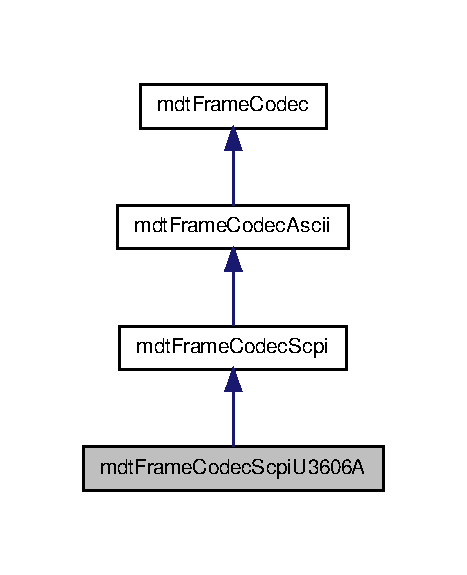
\includegraphics[width=224pt]{classmdt_frame_codec_scpi_u3606_a__inherit__graph}
\end{center}
\end{figure}


Collaboration diagram for mdtFrameCodecScpiU3606A:\nopagebreak
\begin{figure}[H]
\begin{center}
\leavevmode
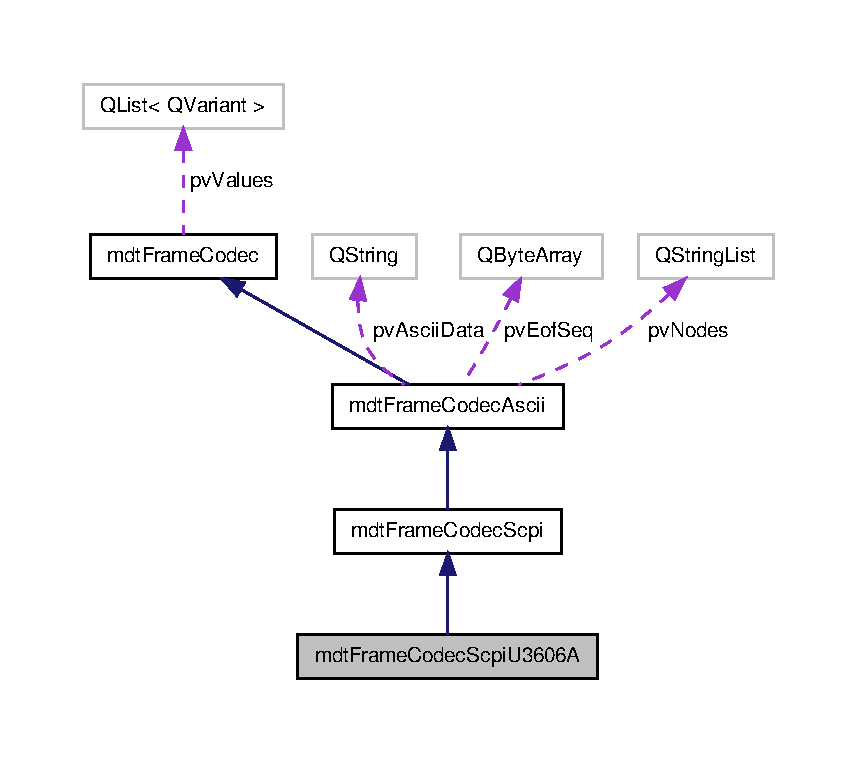
\includegraphics[width=224pt]{classmdt_frame_codec_scpi_u3606_a__coll__graph}
\end{center}
\end{figure}
\subsection*{Public Types}
\begin{DoxyCompactItemize}
\item 
enum \hyperlink{classmdt_frame_codec_scpi_u3606_a_a3d7a1de14d77797a08e3d2991fa9f004}{measure\_\-type\_\-t} \{ \par
\hyperlink{classmdt_frame_codec_scpi_u3606_a_a3d7a1de14d77797a08e3d2991fa9f004a56df4ffec0205d0bae97d56853490eec}{MT\_\-UNKNOW}, 
\hyperlink{classmdt_frame_codec_scpi_u3606_a_a3d7a1de14d77797a08e3d2991fa9f004a7178fed206da47e7f55e68723acf809a}{MT\_\-VOLTAGE\_\-DC}, 
\hyperlink{classmdt_frame_codec_scpi_u3606_a_a3d7a1de14d77797a08e3d2991fa9f004a95fc88c0223637cf3fe3a101fb568f1d}{MT\_\-VOLTAGE\_\-AC}, 
\hyperlink{classmdt_frame_codec_scpi_u3606_a_a3d7a1de14d77797a08e3d2991fa9f004a4b6d05bccb61870ebae4f58c34b41e31}{MT\_\-CURRENT\_\-DC}, 
\par
\hyperlink{classmdt_frame_codec_scpi_u3606_a_a3d7a1de14d77797a08e3d2991fa9f004acecbad4db2f3cb2b92099e2a0f57d3a3}{MT\_\-CURRENT\_\-AC}
 \}
\begin{DoxyCompactList}\small\item\em Measure type. \end{DoxyCompactList}\end{DoxyCompactItemize}
\subsection*{Public Member Functions}
\begin{DoxyCompactItemize}
\item 
bool \hyperlink{classmdt_frame_codec_scpi_u3606_a_adb24e0835c2407e15be1a5a2780f965c}{decodeConfFunc} (QByteArray \&frame)
\begin{DoxyCompactList}\small\item\em Decode the CONFigure and FUNCtion answer. \end{DoxyCompactList}\item 
QVariant \hyperlink{classmdt_frame_codec_scpi_u3606_a_a3ca37c46462e24f9c26d4e352fe2db40}{decodeSingleValueDouble} (QByteArray \&frame)
\begin{DoxyCompactList}\small\item\em Decode a signle value in double floating format. \end{DoxyCompactList}\item 
\hypertarget{classmdt_frame_codec_scpi_u3606_a_a5d2c549ceee92ed152d79b643caab594}{
\hyperlink{classmdt_frame_codec_scpi_u3606_a_a3d7a1de14d77797a08e3d2991fa9f004}{measure\_\-type\_\-t} \hyperlink{classmdt_frame_codec_scpi_u3606_a_a5d2c549ceee92ed152d79b643caab594}{measureType} ()}
\label{classmdt_frame_codec_scpi_u3606_a_a5d2c549ceee92ed152d79b643caab594}

\begin{DoxyCompactList}\small\item\em Get the measure type. \end{DoxyCompactList}\item 
\hypertarget{classmdt_frame_codec_scpi_u3606_a_a2592942192dce715fb828612e2a7e1c9}{
QVariant \hyperlink{classmdt_frame_codec_scpi_u3606_a_a2592942192dce715fb828612e2a7e1c9}{range} ()}
\label{classmdt_frame_codec_scpi_u3606_a_a2592942192dce715fb828612e2a7e1c9}

\begin{DoxyCompactList}\small\item\em Get the measure range. \end{DoxyCompactList}\item 
\hypertarget{classmdt_frame_codec_scpi_u3606_a_a3657c8a712ba324b1d5b10a789a32501}{
QVariant \hyperlink{classmdt_frame_codec_scpi_u3606_a_a3657c8a712ba324b1d5b10a789a32501}{resolution} ()}
\label{classmdt_frame_codec_scpi_u3606_a_a3657c8a712ba324b1d5b10a789a32501}

\begin{DoxyCompactList}\small\item\em Get the measure resolution. \end{DoxyCompactList}\end{DoxyCompactItemize}


\subsection{Detailed Description}
Decode Agilent U3606A SCPI data. 

Definition at line 32 of file mdtFrameCodecScpiU3606A.h.



\subsection{Member Enumeration Documentation}
\hypertarget{classmdt_frame_codec_scpi_u3606_a_a3d7a1de14d77797a08e3d2991fa9f004}{
\index{mdtFrameCodecScpiU3606A@{mdtFrameCodecScpiU3606A}!measure\_\-type\_\-t@{measure\_\-type\_\-t}}
\index{measure\_\-type\_\-t@{measure\_\-type\_\-t}!mdtFrameCodecScpiU3606A@{mdtFrameCodecScpiU3606A}}
\subsubsection[{measure\_\-type\_\-t}]{\setlength{\rightskip}{0pt plus 5cm}enum {\bf mdtFrameCodecScpiU3606A::measure\_\-type\_\-t}}}
\label{classmdt_frame_codec_scpi_u3606_a_a3d7a1de14d77797a08e3d2991fa9f004}


Measure type. 

\begin{Desc}
\item[Enumerator: ]\par
\begin{description}
\index{MT\_\-UNKNOW@{MT\_\-UNKNOW}!mdtFrameCodecScpiU3606A@{mdtFrameCodecScpiU3606A}}\index{mdtFrameCodecScpiU3606A@{mdtFrameCodecScpiU3606A}!MT\_\-UNKNOW@{MT\_\-UNKNOW}}\item[{\em 
\hypertarget{classmdt_frame_codec_scpi_u3606_a_a3d7a1de14d77797a08e3d2991fa9f004a56df4ffec0205d0bae97d56853490eec}{
MT\_\-UNKNOW}
\label{classmdt_frame_codec_scpi_u3606_a_a3d7a1de14d77797a08e3d2991fa9f004a56df4ffec0205d0bae97d56853490eec}
}]Unknow measure type \index{MT\_\-VOLTAGE\_\-DC@{MT\_\-VOLTAGE\_\-DC}!mdtFrameCodecScpiU3606A@{mdtFrameCodecScpiU3606A}}\index{mdtFrameCodecScpiU3606A@{mdtFrameCodecScpiU3606A}!MT\_\-VOLTAGE\_\-DC@{MT\_\-VOLTAGE\_\-DC}}\item[{\em 
\hypertarget{classmdt_frame_codec_scpi_u3606_a_a3d7a1de14d77797a08e3d2991fa9f004a7178fed206da47e7f55e68723acf809a}{
MT\_\-VOLTAGE\_\-DC}
\label{classmdt_frame_codec_scpi_u3606_a_a3d7a1de14d77797a08e3d2991fa9f004a7178fed206da47e7f55e68723acf809a}
}]Measure type DC voltage \index{MT\_\-VOLTAGE\_\-AC@{MT\_\-VOLTAGE\_\-AC}!mdtFrameCodecScpiU3606A@{mdtFrameCodecScpiU3606A}}\index{mdtFrameCodecScpiU3606A@{mdtFrameCodecScpiU3606A}!MT\_\-VOLTAGE\_\-AC@{MT\_\-VOLTAGE\_\-AC}}\item[{\em 
\hypertarget{classmdt_frame_codec_scpi_u3606_a_a3d7a1de14d77797a08e3d2991fa9f004a95fc88c0223637cf3fe3a101fb568f1d}{
MT\_\-VOLTAGE\_\-AC}
\label{classmdt_frame_codec_scpi_u3606_a_a3d7a1de14d77797a08e3d2991fa9f004a95fc88c0223637cf3fe3a101fb568f1d}
}]Measure type AC voltage \index{MT\_\-CURRENT\_\-DC@{MT\_\-CURRENT\_\-DC}!mdtFrameCodecScpiU3606A@{mdtFrameCodecScpiU3606A}}\index{mdtFrameCodecScpiU3606A@{mdtFrameCodecScpiU3606A}!MT\_\-CURRENT\_\-DC@{MT\_\-CURRENT\_\-DC}}\item[{\em 
\hypertarget{classmdt_frame_codec_scpi_u3606_a_a3d7a1de14d77797a08e3d2991fa9f004a4b6d05bccb61870ebae4f58c34b41e31}{
MT\_\-CURRENT\_\-DC}
\label{classmdt_frame_codec_scpi_u3606_a_a3d7a1de14d77797a08e3d2991fa9f004a4b6d05bccb61870ebae4f58c34b41e31}
}]Measure type DC current \index{MT\_\-CURRENT\_\-AC@{MT\_\-CURRENT\_\-AC}!mdtFrameCodecScpiU3606A@{mdtFrameCodecScpiU3606A}}\index{mdtFrameCodecScpiU3606A@{mdtFrameCodecScpiU3606A}!MT\_\-CURRENT\_\-AC@{MT\_\-CURRENT\_\-AC}}\item[{\em 
\hypertarget{classmdt_frame_codec_scpi_u3606_a_a3d7a1de14d77797a08e3d2991fa9f004acecbad4db2f3cb2b92099e2a0f57d3a3}{
MT\_\-CURRENT\_\-AC}
\label{classmdt_frame_codec_scpi_u3606_a_a3d7a1de14d77797a08e3d2991fa9f004acecbad4db2f3cb2b92099e2a0f57d3a3}
}]Measure type AC current \end{description}
\end{Desc}



Definition at line 38 of file mdtFrameCodecScpiU3606A.h.



\subsection{Member Function Documentation}
\hypertarget{classmdt_frame_codec_scpi_u3606_a_adb24e0835c2407e15be1a5a2780f965c}{
\index{mdtFrameCodecScpiU3606A@{mdtFrameCodecScpiU3606A}!decodeConfFunc@{decodeConfFunc}}
\index{decodeConfFunc@{decodeConfFunc}!mdtFrameCodecScpiU3606A@{mdtFrameCodecScpiU3606A}}
\subsubsection[{decodeConfFunc}]{\setlength{\rightskip}{0pt plus 5cm}bool mdtFrameCodecScpiU3606A::decodeConfFunc (
\begin{DoxyParamCaption}
\item[{QByteArray \&}]{frame}
\end{DoxyParamCaption}
)}}
\label{classmdt_frame_codec_scpi_u3606_a_adb24e0835c2407e15be1a5a2780f965c}


Decode the CONFigure and FUNCtion answer. 



Definition at line 30 of file mdtFrameCodecScpiU3606A.cpp.

\hypertarget{classmdt_frame_codec_scpi_u3606_a_a3ca37c46462e24f9c26d4e352fe2db40}{
\index{mdtFrameCodecScpiU3606A@{mdtFrameCodecScpiU3606A}!decodeSingleValueDouble@{decodeSingleValueDouble}}
\index{decodeSingleValueDouble@{decodeSingleValueDouble}!mdtFrameCodecScpiU3606A@{mdtFrameCodecScpiU3606A}}
\subsubsection[{decodeSingleValueDouble}]{\setlength{\rightskip}{0pt plus 5cm}QVariant mdtFrameCodecScpiU3606A::decodeSingleValueDouble (
\begin{DoxyParamCaption}
\item[{QByteArray \&}]{frame}
\end{DoxyParamCaption}
)}}
\label{classmdt_frame_codec_scpi_u3606_a_a3ca37c46462e24f9c26d4e352fe2db40}


Decode a signle value in double floating format. 

This method returns a QVariant. QVariant's internal data is converted to double. If value is not valid, the QVariant is cleared, so it is possible to check this with QVariant::isValid(). When decode was done, the values are available with \hyperlink{classmdt_frame_codec_a2c0cc0f9d9b72ef2295b7ec7eca72ea7}{values()} 

Definition at line 79 of file mdtFrameCodecScpiU3606A.cpp.



The documentation for this class was generated from the following files:\begin{DoxyCompactItemize}
\item 
src/mdtutils/mdtFrameCodecScpiU3606A.h\item 
src/mdtutils/mdtFrameCodecScpiU3606A.cpp\end{DoxyCompactItemize}

\hypertarget{classmdt_frame_modbus_tcp}{
\section{mdtFrameModbusTcp Class Reference}
\label{classmdt_frame_modbus_tcp}\index{mdtFrameModbusTcp@{mdtFrameModbusTcp}}
}


MODBUS/TCP Frame.  




{\ttfamily \#include $<$mdtFrameModbusTcp.h$>$}



Inheritance diagram for mdtFrameModbusTcp:
\nopagebreak
\begin{figure}[H]
\begin{center}
\leavevmode
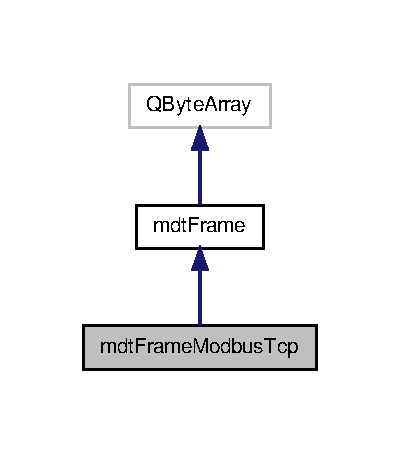
\includegraphics[width=192pt]{classmdt_frame_modbus_tcp__inherit__graph}
\end{center}
\end{figure}


Collaboration diagram for mdtFrameModbusTcp:
\nopagebreak
\begin{figure}[H]
\begin{center}
\leavevmode
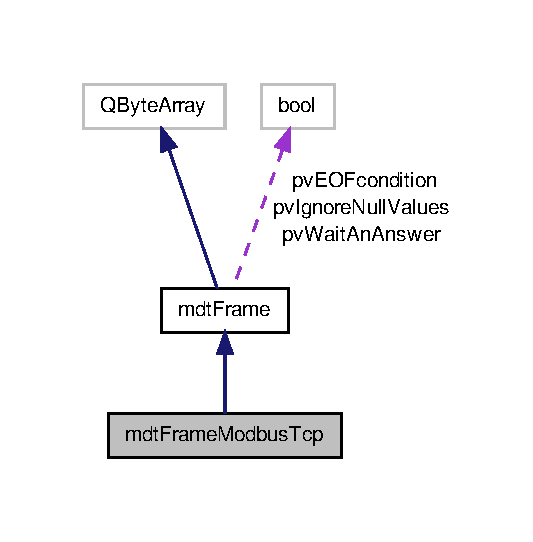
\includegraphics[width=192pt]{classmdt_frame_modbus_tcp__coll__graph}
\end{center}
\end{figure}
\subsection*{Public Member Functions}
\begin{DoxyCompactItemize}
\item 
void \hyperlink{classmdt_frame_modbus_tcp_a622fd5104f4e91a96621e6b5e0f4f89f}{clear} ()
\item 
int \hyperlink{classmdt_frame_modbus_tcp_a0f684d77c03e5fb91598c9a10715bedb}{putData} (const char $\ast$data, int maxLen)
\begin{DoxyCompactList}\small\item\em Overload of \hyperlink{classmdt_frame_a51c355541b134e6e051167c70c09d531}{mdtFrame::putData()} \end{DoxyCompactList}\item 
\hypertarget{classmdt_frame_modbus_tcp_a3c5528d2e45111ec0563dfd3350177cd}{
void \hyperlink{classmdt_frame_modbus_tcp_a3c5528d2e45111ec0563dfd3350177cd}{setTransactionId} (quint16 id)}
\label{classmdt_frame_modbus_tcp_a3c5528d2e45111ec0563dfd3350177cd}

\begin{DoxyCompactList}\small\item\em Set the transaction ID. \end{DoxyCompactList}\item 
\hypertarget{classmdt_frame_modbus_tcp_a48a7e24190190da0ae9f5dbdfcd1ee48}{
quint16 \hyperlink{classmdt_frame_modbus_tcp_a48a7e24190190da0ae9f5dbdfcd1ee48}{transactionId} ()}
\label{classmdt_frame_modbus_tcp_a48a7e24190190da0ae9f5dbdfcd1ee48}

\begin{DoxyCompactList}\small\item\em Get the transaction ID. \end{DoxyCompactList}\item 
\hypertarget{classmdt_frame_modbus_tcp_a5213eb7e3670a191d2b75c83f5dd8d71}{
quint16 \hyperlink{classmdt_frame_modbus_tcp_a5213eb7e3670a191d2b75c83f5dd8d71}{modbusLength} ()}
\label{classmdt_frame_modbus_tcp_a5213eb7e3670a191d2b75c83f5dd8d71}

\begin{DoxyCompactList}\small\item\em Get the length of Unit ID + PDU. \end{DoxyCompactList}\item 
\hypertarget{classmdt_frame_modbus_tcp_ab6bb1765abd0910c6511954a17526243}{
void \hyperlink{classmdt_frame_modbus_tcp_ab6bb1765abd0910c6511954a17526243}{setUnitId} (quint8 id)}
\label{classmdt_frame_modbus_tcp_ab6bb1765abd0910c6511954a17526243}

\begin{DoxyCompactList}\small\item\em Set the Unit ID. \end{DoxyCompactList}\item 
\hypertarget{classmdt_frame_modbus_tcp_a8c2dad33c79f04fd11658ac0cefdf268}{
quint8 \hyperlink{classmdt_frame_modbus_tcp_a8c2dad33c79f04fd11658ac0cefdf268}{unitId} ()}
\label{classmdt_frame_modbus_tcp_a8c2dad33c79f04fd11658ac0cefdf268}

\begin{DoxyCompactList}\small\item\em Get the Unit ID. \end{DoxyCompactList}\item 
\hypertarget{classmdt_frame_modbus_tcp_a171095fd7a250428e4702cf9bc7620d9}{
void \hyperlink{classmdt_frame_modbus_tcp_a171095fd7a250428e4702cf9bc7620d9}{setPdu} (const QByteArray \&pdu)}
\label{classmdt_frame_modbus_tcp_a171095fd7a250428e4702cf9bc7620d9}

\begin{DoxyCompactList}\small\item\em Set the MODBUS PDU. \end{DoxyCompactList}\item 
\hypertarget{classmdt_frame_modbus_tcp_a4462aed344dcd794274a01f837a70d42}{
QByteArray \hyperlink{classmdt_frame_modbus_tcp_a4462aed344dcd794274a01f837a70d42}{getPdu} ()}
\label{classmdt_frame_modbus_tcp_a4462aed344dcd794274a01f837a70d42}

\begin{DoxyCompactList}\small\item\em Get the MODBUS PDU. \end{DoxyCompactList}\item 
void \hyperlink{classmdt_frame_modbus_tcp_a59488845873981f0e2e8f2ffd544e2f4}{encode} ()
\begin{DoxyCompactList}\small\item\em Encode the MODBUS/TCP frame. \end{DoxyCompactList}\end{DoxyCompactItemize}


\subsection{Detailed Description}
MODBUS/TCP Frame. 

This encode/decode a MODBUS/TCP frame. Note that function codes, ... , are not handled here. This application layer functions must be done with a frame codec.

Ref:
\begin{DoxyItemize}
\item MODBUS Messaging on TCP/IP Implementation Guide V1.0b
\item MODBUS Application Protocol Specification V1.1b
\item \href{http://www.Modbus-IDA.org}{\tt http://www.Modbus-\/IDA.org} 
\end{DoxyItemize}

\subsection{Member Function Documentation}
\hypertarget{classmdt_frame_modbus_tcp_a622fd5104f4e91a96621e6b5e0f4f89f}{
\index{mdtFrameModbusTcp@{mdtFrameModbusTcp}!clear@{clear}}
\index{clear@{clear}!mdtFrameModbusTcp@{mdtFrameModbusTcp}}
\subsubsection[{clear}]{\setlength{\rightskip}{0pt plus 5cm}void mdtFrameModbusTcp::clear (
\begin{DoxyParamCaption}
{}
\end{DoxyParamCaption}
)\hspace{0.3cm}{\ttfamily  \mbox{[}virtual\mbox{]}}}}
\label{classmdt_frame_modbus_tcp_a622fd5104f4e91a96621e6b5e0f4f89f}
Clear internal data

Reset internal data and calls \hyperlink{classmdt_frame_acdf8a921a3f36ca91af88b55b90febdc}{mdtFrame::clear()} 

Reimplemented from \hyperlink{classmdt_frame_acdf8a921a3f36ca91af88b55b90febdc}{mdtFrame}.

\hypertarget{classmdt_frame_modbus_tcp_a59488845873981f0e2e8f2ffd544e2f4}{
\index{mdtFrameModbusTcp@{mdtFrameModbusTcp}!encode@{encode}}
\index{encode@{encode}!mdtFrameModbusTcp@{mdtFrameModbusTcp}}
\subsubsection[{encode}]{\setlength{\rightskip}{0pt plus 5cm}void mdtFrameModbusTcp::encode (
\begin{DoxyParamCaption}
{}
\end{DoxyParamCaption}
)}}
\label{classmdt_frame_modbus_tcp_a59488845873981f0e2e8f2ffd544e2f4}


Encode the MODBUS/TCP frame. 

This will build the frame with MBAP Header. Note: \hyperlink{classmdt_frame_modbus_tcp_a622fd5104f4e91a96621e6b5e0f4f89f}{clear()} is called internally of this method. \begin{DoxyPrecond}{Precondition}
Capacity must be $>$= 7 
\end{DoxyPrecond}
\hypertarget{classmdt_frame_modbus_tcp_a0f684d77c03e5fb91598c9a10715bedb}{
\index{mdtFrameModbusTcp@{mdtFrameModbusTcp}!putData@{putData}}
\index{putData@{putData}!mdtFrameModbusTcp@{mdtFrameModbusTcp}}
\subsubsection[{putData}]{\setlength{\rightskip}{0pt plus 5cm}int mdtFrameModbusTcp::putData (
\begin{DoxyParamCaption}
\item[{const char $\ast$}]{data, }
\item[{int}]{maxLen}
\end{DoxyParamCaption}
)}}
\label{classmdt_frame_modbus_tcp_a0f684d77c03e5fb91598c9a10715bedb}


Overload of \hyperlink{classmdt_frame_a51c355541b134e6e051167c70c09d531}{mdtFrame::putData()} 

\begin{DoxyPrecond}{Precondition}
Capacity must be $>$= 7 
\end{DoxyPrecond}
\begin{DoxySeeAlso}{See also}
\hyperlink{classmdt_frame}{mdtFrame} 
\end{DoxySeeAlso}


qDebug() $<$$<$ \char`\"{}mdtFrameModbusTcp::putData(): maxLen (1): \char`\"{} $<$$<$ maxLen;

qDebug() $<$$<$ \char`\"{}mdtFrameModbusTcp::putData(): stored(1): \char`\"{} $<$$<$ stored $<$$<$ \char`\"{} , maxLen (2): \char`\"{} $<$$<$ maxLen;

qDebug() $<$$<$ \char`\"{}mdtFrameModbusTcp::putData(): maxLen (3): \char`\"{} $<$$<$ maxLen;

qDebug() $<$$<$ \char`\"{}mdtFrameModbusTcp::putData(): maxLen (4): \char`\"{} $<$$<$ maxLen;

qDebug() $<$$<$ \char`\"{}mdtFrameModbusTcp::putData(): stored: \char`\"{} $<$$<$ stored; 



The documentation for this class was generated from the following files:\begin{DoxyCompactItemize}
\item 
src/mdtutils/mdtFrameModbusTcp.h\item 
src/mdtutils/mdtFrameModbusTcp.cpp\end{DoxyCompactItemize}

\hypertarget{classmdt_led}{\section{mdt\-Led Class Reference}
\label{classmdt_led}\index{mdt\-Led@{mdt\-Led}}
}


mdt\-L\-E\-D is a widget witch displays a L\-E\-D  




{\ttfamily \#include $<$mdt\-Led.\-h$>$}



Inheritance diagram for mdt\-Led\-:\nopagebreak
\begin{figure}[H]
\begin{center}
\leavevmode
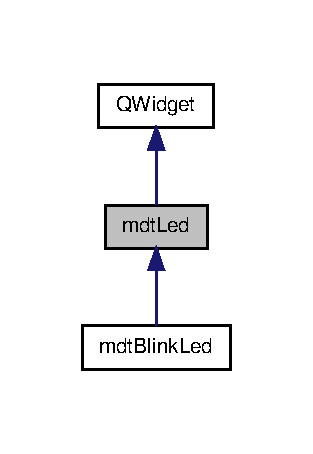
\includegraphics[width=150pt]{classmdt_led__inherit__graph}
\end{center}
\end{figure}


Collaboration diagram for mdt\-Led\-:\nopagebreak
\begin{figure}[H]
\begin{center}
\leavevmode
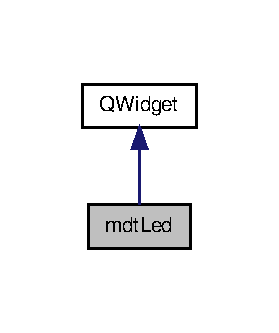
\includegraphics[width=134pt]{classmdt_led__coll__graph}
\end{center}
\end{figure}
\subsection*{Public Types}
\begin{DoxyCompactItemize}
\item 
enum \hyperlink{classmdt_led_a2d57d9ef04d2105d2fad93b57fc7cfef}{color\-\_\-t} \{ \hyperlink{classmdt_led_a2d57d9ef04d2105d2fad93b57fc7cfefa45b61a84d67fbd6379dee70b59193415}{Green}, 
\hyperlink{classmdt_led_a2d57d9ef04d2105d2fad93b57fc7cfefa5dc598374ab643ab42ea786bc7fe4a04}{Orange}, 
\hyperlink{classmdt_led_a2d57d9ef04d2105d2fad93b57fc7cfefab889f9da8e6cf657379cb521c3d11406}{Red}
 \}
\begin{DoxyCompactList}\small\item\em L\-E\-D predefined colors. \end{DoxyCompactList}\end{DoxyCompactItemize}
\subsection*{Public Slots}
\begin{DoxyCompactItemize}
\item 
void \hyperlink{classmdt_led_a389ee3e0082ce8fa38cb258944a04892}{set\-On} ()
\begin{DoxyCompactList}\small\item\em Set the L\-E\-D O\-N. \end{DoxyCompactList}\item 
void \hyperlink{classmdt_led_a4c8f5f6aa91b7c90ae6b1aa4933ba6e0}{set\-Off} ()
\begin{DoxyCompactList}\small\item\em Set the L\-E\-D O\-F\-F. \end{DoxyCompactList}\item 
void \hyperlink{classmdt_led_aabbe7fcb23d539946dffec4526c89495}{set\-On} (bool on)
\begin{DoxyCompactList}\small\item\em Set the L\-E\-D O\-N or O\-F\-F. \end{DoxyCompactList}\item 
void \hyperlink{classmdt_led_a9e86ff65f2ec1bfb6131e2b9042609e8}{toggle\-On\-Off} ()
\begin{DoxyCompactList}\small\item\em Toggle On/\-Off. \end{DoxyCompactList}\end{DoxyCompactItemize}
\subsection*{Public Member Functions}
\begin{DoxyCompactItemize}
\item 
\hyperlink{classmdt_led_a64d5de3a8c2e4937d9ca9328b5ae4f9c}{mdt\-Led} (\hyperlink{class_q_widget}{Q\-Widget} $\ast$parent=0)
\begin{DoxyCompactList}\small\item\em Contruct a new mdt\-L\-E\-D. \end{DoxyCompactList}\item 
void \hyperlink{classmdt_led_a1271e1dfe07e8ff459d7f20e55ab3bc4}{set\-Borders} (int horizontal\-Border, int vertical\-Border)
\begin{DoxyCompactList}\small\item\em Set the borders. \end{DoxyCompactList}\item 
void \hyperlink{classmdt_led_a5f3b4975c423ac35442ec2b9c546b0e4}{set\-Green} ()
\begin{DoxyCompactList}\small\item\em Set the L\-E\-D color to green. \end{DoxyCompactList}\item 
void \hyperlink{classmdt_led_a5cdd40d1e3baefab72d9cda866353797}{set\-Orange} ()
\begin{DoxyCompactList}\small\item\em Set the L\-E\-D color to orange. \end{DoxyCompactList}\item 
void \hyperlink{classmdt_led_a28e208fb105c99b21d81d4c82ed50a98}{set\-Red} ()
\begin{DoxyCompactList}\small\item\em Set the L\-E\-D color to red. \end{DoxyCompactList}\item 
void \hyperlink{classmdt_led_a16e89edb08321c7abec736b2ebf28986}{set\-Color} (\hyperlink{classmdt_led_a2d57d9ef04d2105d2fad93b57fc7cfef}{color\-\_\-t} color)
\begin{DoxyCompactList}\small\item\em Set the L\-E\-D color. \end{DoxyCompactList}\item 
void \hyperlink{classmdt_led_a664ca4c83ec0faaa86bd3f932fb06d5b}{set\-Flat} ()
\begin{DoxyCompactList}\small\item\em Set a simple flat L\-E\-D. \end{DoxyCompactList}\item 
void \hyperlink{classmdt_led_a8ec814fdc4910476e7479649ba3f6204}{set\-Glint} ()
\begin{DoxyCompactList}\small\item\em Set a glint L\-E\-D. \end{DoxyCompactList}\item 
void \hyperlink{classmdt_led_a6aabb78ea686814f316f88e20d024d39}{set\-Text\-Mode} ()
\begin{DoxyCompactList}\small\item\em Set the L\-E\-D as text. \end{DoxyCompactList}\item 
void \hyperlink{classmdt_led_ab8a997e610a2ad5572e1a6dbe7fbc256}{set\-Antialiasing} (bool enabled)
\begin{DoxyCompactList}\small\item\em Enable the antialiasing. \end{DoxyCompactList}\item 
void \hyperlink{classmdt_led_abd0fde0ce1eca75fe7c832557829089b}{set\-Fixed\-Size} (int width, int height)
\begin{DoxyCompactList}\small\item\em Force the L\-E\-D to have a fixed size. \end{DoxyCompactList}\item 
void \hyperlink{classmdt_led_a696570e6eb8f5b0a629fc6823ed2fe4d}{set\-Auto\-Size} ()
\begin{DoxyCompactList}\small\item\em Use Qt Q\-Size\-Policy to resize the L\-E\-D. \end{DoxyCompactList}\item 
Q\-Size \hyperlink{classmdt_led_a44cf6e19e2640bc843d1ed096843e686}{size\-Hint} () const 
\item 
Q\-Size \hyperlink{classmdt_led_ae7d22257f19d57771299b321a8a17c50}{minimum\-Size\-Hint} () const 
\item 
bool \hyperlink{classmdt_led_a97c9b46867c260cb27901e2968146809}{is\-On} ()
\begin{DoxyCompactList}\small\item\em Get the L\-E\-D O\-N state. \end{DoxyCompactList}\end{DoxyCompactItemize}
\subsection*{Protected Member Functions}
\begin{DoxyCompactItemize}
\item 
void \hyperlink{classmdt_led_a1c96c8e06658ba569f7cf6b3fc3f5903}{paint\-Event} (Q\-Paint\-Event $\ast$)
\end{DoxyCompactItemize}


\subsection{Detailed Description}
mdt\-L\-E\-D is a widget witch displays a L\-E\-D 



Definition at line 35 of file mdt\-Led.\-h.



\subsection{Member Enumeration Documentation}
\hypertarget{classmdt_led_a2d57d9ef04d2105d2fad93b57fc7cfef}{\index{mdt\-Led@{mdt\-Led}!color\-\_\-t@{color\-\_\-t}}
\index{color\-\_\-t@{color\-\_\-t}!mdtLed@{mdt\-Led}}
\subsubsection[{color\-\_\-t}]{\setlength{\rightskip}{0pt plus 5cm}enum {\bf mdt\-Led\-::color\-\_\-t}}}\label{classmdt_led_a2d57d9ef04d2105d2fad93b57fc7cfef}


L\-E\-D predefined colors. 

\begin{Desc}
\item[Enumerator]\par
\begin{description}
\index{Green@{Green}!mdt\-Led@{mdt\-Led}}\index{mdt\-Led@{mdt\-Led}!Green@{Green}}\item[{\em 
\hypertarget{classmdt_led_a2d57d9ef04d2105d2fad93b57fc7cfefa45b61a84d67fbd6379dee70b59193415}{Green}\label{classmdt_led_a2d57d9ef04d2105d2fad93b57fc7cfefa45b61a84d67fbd6379dee70b59193415}
}]Green L\-E\-D \index{Orange@{Orange}!mdt\-Led@{mdt\-Led}}\index{mdt\-Led@{mdt\-Led}!Orange@{Orange}}\item[{\em 
\hypertarget{classmdt_led_a2d57d9ef04d2105d2fad93b57fc7cfefa5dc598374ab643ab42ea786bc7fe4a04}{Orange}\label{classmdt_led_a2d57d9ef04d2105d2fad93b57fc7cfefa5dc598374ab643ab42ea786bc7fe4a04}
}]Orange L\-E\-D \index{Red@{Red}!mdt\-Led@{mdt\-Led}}\index{mdt\-Led@{mdt\-Led}!Red@{Red}}\item[{\em 
\hypertarget{classmdt_led_a2d57d9ef04d2105d2fad93b57fc7cfefab889f9da8e6cf657379cb521c3d11406}{Red}\label{classmdt_led_a2d57d9ef04d2105d2fad93b57fc7cfefab889f9da8e6cf657379cb521c3d11406}
}]Red L\-E\-D \end{description}
\end{Desc}


Definition at line 43 of file mdt\-Led.\-h.



\subsection{Constructor \& Destructor Documentation}
\hypertarget{classmdt_led_a64d5de3a8c2e4937d9ca9328b5ae4f9c}{\index{mdt\-Led@{mdt\-Led}!mdt\-Led@{mdt\-Led}}
\index{mdt\-Led@{mdt\-Led}!mdtLed@{mdt\-Led}}
\subsubsection[{mdt\-Led}]{\setlength{\rightskip}{0pt plus 5cm}mdt\-Led\-::mdt\-Led (
\begin{DoxyParamCaption}
\item[{{\bf Q\-Widget} $\ast$}]{parent = {\ttfamily 0}}
\end{DoxyParamCaption}
)}}\label{classmdt_led_a64d5de3a8c2e4937d9ca9328b5ae4f9c}


Contruct a new mdt\-L\-E\-D. 



Definition at line 27 of file mdt\-Led.\-cpp.



References set\-Borders(), set\-Glint(), set\-Green(), and set\-Off().



\subsection{Member Function Documentation}
\hypertarget{classmdt_led_a97c9b46867c260cb27901e2968146809}{\index{mdt\-Led@{mdt\-Led}!is\-On@{is\-On}}
\index{is\-On@{is\-On}!mdtLed@{mdt\-Led}}
\subsubsection[{is\-On}]{\setlength{\rightskip}{0pt plus 5cm}bool mdt\-Led\-::is\-On (
\begin{DoxyParamCaption}
{}
\end{DoxyParamCaption}
)}}\label{classmdt_led_a97c9b46867c260cb27901e2968146809}


Get the L\-E\-D O\-N state. 



Definition at line 155 of file mdt\-Led.\-cpp.

\hypertarget{classmdt_led_ae7d22257f19d57771299b321a8a17c50}{\index{mdt\-Led@{mdt\-Led}!minimum\-Size\-Hint@{minimum\-Size\-Hint}}
\index{minimum\-Size\-Hint@{minimum\-Size\-Hint}!mdtLed@{mdt\-Led}}
\subsubsection[{minimum\-Size\-Hint}]{\setlength{\rightskip}{0pt plus 5cm}Q\-Size mdt\-Led\-::minimum\-Size\-Hint (
\begin{DoxyParamCaption}
{}
\end{DoxyParamCaption}
) const}}\label{classmdt_led_ae7d22257f19d57771299b321a8a17c50}


Definition at line 150 of file mdt\-Led.\-cpp.

\hypertarget{classmdt_led_a1c96c8e06658ba569f7cf6b3fc3f5903}{\index{mdt\-Led@{mdt\-Led}!paint\-Event@{paint\-Event}}
\index{paint\-Event@{paint\-Event}!mdtLed@{mdt\-Led}}
\subsubsection[{paint\-Event}]{\setlength{\rightskip}{0pt plus 5cm}void mdt\-Led\-::paint\-Event (
\begin{DoxyParamCaption}
\item[{Q\-Paint\-Event $\ast$}]{}
\end{DoxyParamCaption}
)\hspace{0.3cm}{\ttfamily [protected]}}}\label{classmdt_led_a1c96c8e06658ba569f7cf6b3fc3f5903}


Definition at line 196 of file mdt\-Led.\-cpp.

\hypertarget{classmdt_led_ab8a997e610a2ad5572e1a6dbe7fbc256}{\index{mdt\-Led@{mdt\-Led}!set\-Antialiasing@{set\-Antialiasing}}
\index{set\-Antialiasing@{set\-Antialiasing}!mdtLed@{mdt\-Led}}
\subsubsection[{set\-Antialiasing}]{\setlength{\rightskip}{0pt plus 5cm}void mdt\-Led\-::set\-Antialiasing (
\begin{DoxyParamCaption}
\item[{bool}]{enabled}
\end{DoxyParamCaption}
)}}\label{classmdt_led_ab8a997e610a2ad5572e1a6dbe7fbc256}


Enable the antialiasing. 


\begin{DoxyParams}{Parameters}
{\em enabled} & If true, antialiasing will be enabled (else, diseabled) \\
\hline
\end{DoxyParams}


Definition at line 114 of file mdt\-Led.\-cpp.

\hypertarget{classmdt_led_a696570e6eb8f5b0a629fc6823ed2fe4d}{\index{mdt\-Led@{mdt\-Led}!set\-Auto\-Size@{set\-Auto\-Size}}
\index{set\-Auto\-Size@{set\-Auto\-Size}!mdtLed@{mdt\-Led}}
\subsubsection[{set\-Auto\-Size}]{\setlength{\rightskip}{0pt plus 5cm}void mdt\-Led\-::set\-Auto\-Size (
\begin{DoxyParamCaption}
{}
\end{DoxyParamCaption}
)}}\label{classmdt_led_a696570e6eb8f5b0a629fc6823ed2fe4d}


Use Qt Q\-Size\-Policy to resize the L\-E\-D. 

Use the Qt default Q\-Size\-Policy (see the Q\-Layout and \hyperlink{class_q_widget}{Q\-Widget} references for details) This is the default behaviour if \hyperlink{classmdt_led_abd0fde0ce1eca75fe7c832557829089b}{set\-Fixed\-Size()} was never called. 

Definition at line 136 of file mdt\-Led.\-cpp.

\hypertarget{classmdt_led_a1271e1dfe07e8ff459d7f20e55ab3bc4}{\index{mdt\-Led@{mdt\-Led}!set\-Borders@{set\-Borders}}
\index{set\-Borders@{set\-Borders}!mdtLed@{mdt\-Led}}
\subsubsection[{set\-Borders}]{\setlength{\rightskip}{0pt plus 5cm}void mdt\-Led\-::set\-Borders (
\begin{DoxyParamCaption}
\item[{int}]{horizontal\-Border, }
\item[{int}]{vertical\-Border}
\end{DoxyParamCaption}
)}}\label{classmdt_led_a1271e1dfe07e8ff459d7f20e55ab3bc4}


Set the borders. 

The L\-E\-D will be drawn in the center, with horizontal and vertical specified spaces. 
\begin{DoxyParams}{Parameters}
{\em horizontal\-Border} & Set the horizontal borders (will be the same at left and right of the L\-E\-D) \\
\hline
{\em vertical\-Border} & Set the vertical borders (will be the same at top and bottom of the L\-E\-D) \\
\hline
\end{DoxyParams}


Definition at line 48 of file mdt\-Led.\-cpp.



Referenced by mdt\-Led().

\hypertarget{classmdt_led_a16e89edb08321c7abec736b2ebf28986}{\index{mdt\-Led@{mdt\-Led}!set\-Color@{set\-Color}}
\index{set\-Color@{set\-Color}!mdtLed@{mdt\-Led}}
\subsubsection[{set\-Color}]{\setlength{\rightskip}{0pt plus 5cm}void mdt\-Led\-::set\-Color (
\begin{DoxyParamCaption}
\item[{{\bf mdt\-Led\-::color\-\_\-t}}]{color}
\end{DoxyParamCaption}
)}}\label{classmdt_led_a16e89edb08321c7abec736b2ebf28986}


Set the L\-E\-D color. 



Definition at line 83 of file mdt\-Led.\-cpp.



References Green, Orange, Red, set\-Green(), set\-Orange(), and set\-Red().



Referenced by mdt\-Port\-Status\-Widget\-::set\-State().

\hypertarget{classmdt_led_abd0fde0ce1eca75fe7c832557829089b}{\index{mdt\-Led@{mdt\-Led}!set\-Fixed\-Size@{set\-Fixed\-Size}}
\index{set\-Fixed\-Size@{set\-Fixed\-Size}!mdtLed@{mdt\-Led}}
\subsubsection[{set\-Fixed\-Size}]{\setlength{\rightskip}{0pt plus 5cm}void mdt\-Led\-::set\-Fixed\-Size (
\begin{DoxyParamCaption}
\item[{int}]{width, }
\item[{int}]{height}
\end{DoxyParamCaption}
)}}\label{classmdt_led_abd0fde0ce1eca75fe7c832557829089b}


Force the L\-E\-D to have a fixed size. 

By default, ldt\-L\-E\-D uses the Qt default Q\-Size\-Policy Wenn calling this method, the L\-E\-D will keep a fixed size 
\begin{DoxyParams}{Parameters}
{\em width} & The width (min. 10) \\
\hline
{\em height} & The height (min. 10) \\
\hline
\end{DoxyParams}


Definition at line 119 of file mdt\-Led.\-cpp.



Referenced by mdt\-Port\-Status\-Widget\-::enable\-Tx\-Rx\-Leds(), mdt\-Digital\-In\-Widget\-::mdt\-Digital\-In\-Widget(), mdt\-Port\-Status\-Widget\-::mdt\-Port\-Status\-Widget(), and mdt\-Serial\-Port\-Ctl\-Widget\-::mdt\-Serial\-Port\-Ctl\-Widget().

\hypertarget{classmdt_led_a664ca4c83ec0faaa86bd3f932fb06d5b}{\index{mdt\-Led@{mdt\-Led}!set\-Flat@{set\-Flat}}
\index{set\-Flat@{set\-Flat}!mdtLed@{mdt\-Led}}
\subsubsection[{set\-Flat}]{\setlength{\rightskip}{0pt plus 5cm}void mdt\-Led\-::set\-Flat (
\begin{DoxyParamCaption}
{}
\end{DoxyParamCaption}
)}}\label{classmdt_led_a664ca4c83ec0faaa86bd3f932fb06d5b}


Set a simple flat L\-E\-D. 

The color will be uniform on the L\-E\-D surface 

Definition at line 98 of file mdt\-Led.\-cpp.

\hypertarget{classmdt_led_a8ec814fdc4910476e7479649ba3f6204}{\index{mdt\-Led@{mdt\-Led}!set\-Glint@{set\-Glint}}
\index{set\-Glint@{set\-Glint}!mdtLed@{mdt\-Led}}
\subsubsection[{set\-Glint}]{\setlength{\rightskip}{0pt plus 5cm}void mdt\-Led\-::set\-Glint (
\begin{DoxyParamCaption}
{}
\end{DoxyParamCaption}
)}}\label{classmdt_led_a8ec814fdc4910476e7479649ba3f6204}


Set a glint L\-E\-D. 

This will use the Qt\-::\-Radial\-Gradient\-Pattern brush style This can slow down the application with many L\-E\-D's. For better performance, use \hyperlink{classmdt_led_a664ca4c83ec0faaa86bd3f932fb06d5b}{set\-Flat()} . 

Definition at line 104 of file mdt\-Led.\-cpp.



Referenced by mdt\-Led().

\hypertarget{classmdt_led_a5f3b4975c423ac35442ec2b9c546b0e4}{\index{mdt\-Led@{mdt\-Led}!set\-Green@{set\-Green}}
\index{set\-Green@{set\-Green}!mdtLed@{mdt\-Led}}
\subsubsection[{set\-Green}]{\setlength{\rightskip}{0pt plus 5cm}void mdt\-Led\-::set\-Green (
\begin{DoxyParamCaption}
{}
\end{DoxyParamCaption}
)}}\label{classmdt_led_a5f3b4975c423ac35442ec2b9c546b0e4}


Set the L\-E\-D color to green. 



Definition at line 56 of file mdt\-Led.\-cpp.



Referenced by mdt\-Port\-Status\-Widget\-::enable\-Tx\-Rx\-Leds(), mdt\-Led(), and set\-Color().

\hypertarget{classmdt_led_a4c8f5f6aa91b7c90ae6b1aa4933ba6e0}{\index{mdt\-Led@{mdt\-Led}!set\-Off@{set\-Off}}
\index{set\-Off@{set\-Off}!mdtLed@{mdt\-Led}}
\subsubsection[{set\-Off}]{\setlength{\rightskip}{0pt plus 5cm}void mdt\-Led\-::set\-Off (
\begin{DoxyParamCaption}
{}
\end{DoxyParamCaption}
)\hspace{0.3cm}{\ttfamily [slot]}}}\label{classmdt_led_a4c8f5f6aa91b7c90ae6b1aa4933ba6e0}


Set the L\-E\-D O\-F\-F. 



Definition at line 169 of file mdt\-Led.\-cpp.



Referenced by mdt\-Led(), mdt\-Blink\-Led\-::set\-Off(), set\-On(), and toggle\-On\-Off().

\hypertarget{classmdt_led_a389ee3e0082ce8fa38cb258944a04892}{\index{mdt\-Led@{mdt\-Led}!set\-On@{set\-On}}
\index{set\-On@{set\-On}!mdtLed@{mdt\-Led}}
\subsubsection[{set\-On}]{\setlength{\rightskip}{0pt plus 5cm}void mdt\-Led\-::set\-On (
\begin{DoxyParamCaption}
{}
\end{DoxyParamCaption}
)\hspace{0.3cm}{\ttfamily [slot]}}}\label{classmdt_led_a389ee3e0082ce8fa38cb258944a04892}


Set the L\-E\-D O\-N. 



Definition at line 160 of file mdt\-Led.\-cpp.



Referenced by mdt\-Blink\-Led\-::set\-On(), set\-On(), and toggle\-On\-Off().

\hypertarget{classmdt_led_aabbe7fcb23d539946dffec4526c89495}{\index{mdt\-Led@{mdt\-Led}!set\-On@{set\-On}}
\index{set\-On@{set\-On}!mdtLed@{mdt\-Led}}
\subsubsection[{set\-On}]{\setlength{\rightskip}{0pt plus 5cm}void mdt\-Led\-::set\-On (
\begin{DoxyParamCaption}
\item[{bool}]{on}
\end{DoxyParamCaption}
)\hspace{0.3cm}{\ttfamily [slot]}}}\label{classmdt_led_aabbe7fcb23d539946dffec4526c89495}


Set the L\-E\-D O\-N or O\-F\-F. 


\begin{DoxyParams}{Parameters}
{\em on} & If true, the L\-E\-D is set O\-N , else O\-F\-F \\
\hline
\end{DoxyParams}


Definition at line 178 of file mdt\-Led.\-cpp.



References set\-Off(), and set\-On().

\hypertarget{classmdt_led_a5cdd40d1e3baefab72d9cda866353797}{\index{mdt\-Led@{mdt\-Led}!set\-Orange@{set\-Orange}}
\index{set\-Orange@{set\-Orange}!mdtLed@{mdt\-Led}}
\subsubsection[{set\-Orange}]{\setlength{\rightskip}{0pt plus 5cm}void mdt\-Led\-::set\-Orange (
\begin{DoxyParamCaption}
{}
\end{DoxyParamCaption}
)}}\label{classmdt_led_a5cdd40d1e3baefab72d9cda866353797}


Set the L\-E\-D color to orange. 



Definition at line 65 of file mdt\-Led.\-cpp.



Referenced by set\-Color().

\hypertarget{classmdt_led_a28e208fb105c99b21d81d4c82ed50a98}{\index{mdt\-Led@{mdt\-Led}!set\-Red@{set\-Red}}
\index{set\-Red@{set\-Red}!mdtLed@{mdt\-Led}}
\subsubsection[{set\-Red}]{\setlength{\rightskip}{0pt plus 5cm}void mdt\-Led\-::set\-Red (
\begin{DoxyParamCaption}
{}
\end{DoxyParamCaption}
)}}\label{classmdt_led_a28e208fb105c99b21d81d4c82ed50a98}


Set the L\-E\-D color to red. 



Definition at line 74 of file mdt\-Led.\-cpp.



Referenced by set\-Color().

\hypertarget{classmdt_led_a6aabb78ea686814f316f88e20d024d39}{\index{mdt\-Led@{mdt\-Led}!set\-Text\-Mode@{set\-Text\-Mode}}
\index{set\-Text\-Mode@{set\-Text\-Mode}!mdtLed@{mdt\-Led}}
\subsubsection[{set\-Text\-Mode}]{\setlength{\rightskip}{0pt plus 5cm}void mdt\-Led\-::set\-Text\-Mode (
\begin{DoxyParamCaption}
{}
\end{DoxyParamCaption}
)}}\label{classmdt_led_a6aabb78ea686814f316f88e20d024d39}


Set the L\-E\-D as text. 

The L\-E\-D will display a O\-N/\-O\-F\-F text instead a color 

Definition at line 109 of file mdt\-Led.\-cpp.

\hypertarget{classmdt_led_a44cf6e19e2640bc843d1ed096843e686}{\index{mdt\-Led@{mdt\-Led}!size\-Hint@{size\-Hint}}
\index{size\-Hint@{size\-Hint}!mdtLed@{mdt\-Led}}
\subsubsection[{size\-Hint}]{\setlength{\rightskip}{0pt plus 5cm}Q\-Size mdt\-Led\-::size\-Hint (
\begin{DoxyParamCaption}
{}
\end{DoxyParamCaption}
) const}}\label{classmdt_led_a44cf6e19e2640bc843d1ed096843e686}


Definition at line 145 of file mdt\-Led.\-cpp.

\hypertarget{classmdt_led_a9e86ff65f2ec1bfb6131e2b9042609e8}{\index{mdt\-Led@{mdt\-Led}!toggle\-On\-Off@{toggle\-On\-Off}}
\index{toggle\-On\-Off@{toggle\-On\-Off}!mdtLed@{mdt\-Led}}
\subsubsection[{toggle\-On\-Off}]{\setlength{\rightskip}{0pt plus 5cm}void mdt\-Led\-::toggle\-On\-Off (
\begin{DoxyParamCaption}
{}
\end{DoxyParamCaption}
)\hspace{0.3cm}{\ttfamily [slot]}}}\label{classmdt_led_a9e86ff65f2ec1bfb6131e2b9042609e8}


Toggle On/\-Off. 



Definition at line 187 of file mdt\-Led.\-cpp.



References set\-Off(), and set\-On().



Referenced by mdt\-Blink\-Led\-::mdt\-Blink\-Led().



The documentation for this class was generated from the following files\-:\begin{DoxyCompactItemize}
\item 
src/mdtutilsgui/\hyperlink{mdt_led_8h}{mdt\-Led.\-h}\item 
src/mdtutilsgui/\hyperlink{mdt_led_8cpp}{mdt\-Led.\-cpp}\end{DoxyCompactItemize}

\hypertarget{classmdt_parent_child_table_item}{
\section{mdtParentChildTableItem Class Reference}
\label{classmdt_parent_child_table_item}\index{mdtParentChildTableItem@{mdtParentChildTableItem}}
}


Collaboration diagram for mdtParentChildTableItem:\nopagebreak
\begin{figure}[H]
\begin{center}
\leavevmode
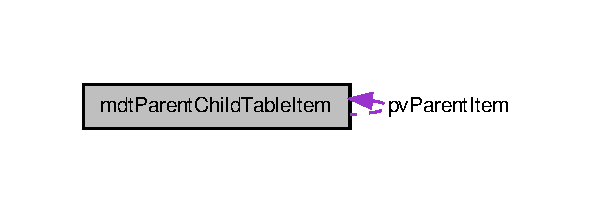
\includegraphics[width=285pt]{classmdt_parent_child_table_item__coll__graph}
\end{center}
\end{figure}
\subsection*{Public Member Functions}
\begin{DoxyCompactItemize}
\item 
\hyperlink{classmdt_parent_child_table_item_afd38823879e25db1dca8099fb138042c}{mdtParentChildTableItem} (QAbstractItemModel $\ast$model, int modelRow, \hyperlink{classmdt_parent_child_table_item}{mdtParentChildTableItem} $\ast$parent)
\begin{DoxyCompactList}\small\item\em Table item constructor. \end{DoxyCompactList}\item 
\hypertarget{classmdt_parent_child_table_item_ad1a5c00ca1d0367d631548fa5732d41c}{
\hyperlink{classmdt_parent_child_table_item_ad1a5c00ca1d0367d631548fa5732d41c}{mdtParentChildTableItem} ()}
\label{classmdt_parent_child_table_item_ad1a5c00ca1d0367d631548fa5732d41c}

\begin{DoxyCompactList}\small\item\em Table item constructor Use this constructor to create the root item of the model. \end{DoxyCompactList}\item 
\hypertarget{classmdt_parent_child_table_item_a182fff209f0a7c9319cbcf72908df69f}{
void {\bfseries appendChild} (\hyperlink{classmdt_parent_child_table_item}{mdtParentChildTableItem} $\ast$child)}
\label{classmdt_parent_child_table_item_a182fff209f0a7c9319cbcf72908df69f}

\item 
\hypertarget{classmdt_parent_child_table_item_ab6c36c72d8eb49fac2035d7e2b9474a3}{
\hyperlink{classmdt_parent_child_table_item}{mdtParentChildTableItem} $\ast$ {\bfseries child} (int row)}
\label{classmdt_parent_child_table_item_ab6c36c72d8eb49fac2035d7e2b9474a3}

\item 
\hypertarget{classmdt_parent_child_table_item_ac2168fc5f960d506f090b7aafcb4fec2}{
int {\bfseries childCount} () const }
\label{classmdt_parent_child_table_item_ac2168fc5f960d506f090b7aafcb4fec2}

\item 
\hypertarget{classmdt_parent_child_table_item_ac4491aa3959249d1a1a6f1582b975589}{
\hyperlink{classmdt_parent_child_table_item}{mdtParentChildTableItem} $\ast$ {\bfseries parent} ()}
\label{classmdt_parent_child_table_item_ac4491aa3959249d1a1a6f1582b975589}

\item 
int \hyperlink{classmdt_parent_child_table_item_aca8d9e7b872c412d67f4125a88312c5a}{columnCount} () const 
\begin{DoxyCompactList}\small\item\em Columns count of the stored model. \end{DoxyCompactList}\item 
QVariant \hyperlink{classmdt_parent_child_table_item_a7150ac4c6a082887e7076f05a37f4781}{data} (int column, int role) const 
\begin{DoxyCompactList}\small\item\em Returns the data of the stored model at stored row The row is set by constructor. \end{DoxyCompactList}\item 
\hypertarget{classmdt_parent_child_table_item_ab2defb25c5033398a6fc4fcd7f015c95}{
int {\bfseries row} () const }
\label{classmdt_parent_child_table_item_ab2defb25c5033398a6fc4fcd7f015c95}

\item 
\hypertarget{classmdt_parent_child_table_item_aceb2319dfd2707cfe8d93705f56bc43c}{
QAbstractItemModel $\ast$ {\bfseries model} ()}
\label{classmdt_parent_child_table_item_aceb2319dfd2707cfe8d93705f56bc43c}

\end{DoxyCompactItemize}


\subsection{Constructor \& Destructor Documentation}
\hypertarget{classmdt_parent_child_table_item_afd38823879e25db1dca8099fb138042c}{
\index{mdtParentChildTableItem@{mdtParentChildTableItem}!mdtParentChildTableItem@{mdtParentChildTableItem}}
\index{mdtParentChildTableItem@{mdtParentChildTableItem}!mdtParentChildTableItem@{mdtParentChildTableItem}}
\subsubsection[{mdtParentChildTableItem}]{\setlength{\rightskip}{0pt plus 5cm}mdtParentChildTableItem::mdtParentChildTableItem (
\begin{DoxyParamCaption}
\item[{QAbstractItemModel $\ast$}]{model, }
\item[{int}]{modelRow, }
\item[{{\bf mdtParentChildTableItem} $\ast$}]{parent}
\end{DoxyParamCaption}
)}}
\label{classmdt_parent_child_table_item_afd38823879e25db1dca8099fb138042c}


Table item constructor. 


\begin{DoxyParams}{Parameters}
{\em parent} & Set the parent reference of this object \\
\hline
{\em model} & The table model to reference (let it null when creating the root object) \\
\hline
{\em modelRow} & Set the row from the model that must be referenced \\
\hline
\end{DoxyParams}


\subsection{Member Function Documentation}
\hypertarget{classmdt_parent_child_table_item_aca8d9e7b872c412d67f4125a88312c5a}{
\index{mdtParentChildTableItem@{mdtParentChildTableItem}!columnCount@{columnCount}}
\index{columnCount@{columnCount}!mdtParentChildTableItem@{mdtParentChildTableItem}}
\subsubsection[{columnCount}]{\setlength{\rightskip}{0pt plus 5cm}int mdtParentChildTableItem::columnCount (
\begin{DoxyParamCaption}
{}
\end{DoxyParamCaption}
) const}}
\label{classmdt_parent_child_table_item_aca8d9e7b872c412d67f4125a88312c5a}


Columns count of the stored model. 

\begin{DoxyReturn}{Returns}
Columns count of the stored model 
\end{DoxyReturn}
\hypertarget{classmdt_parent_child_table_item_a7150ac4c6a082887e7076f05a37f4781}{
\index{mdtParentChildTableItem@{mdtParentChildTableItem}!data@{data}}
\index{data@{data}!mdtParentChildTableItem@{mdtParentChildTableItem}}
\subsubsection[{data}]{\setlength{\rightskip}{0pt plus 5cm}QVariant mdtParentChildTableItem::data (
\begin{DoxyParamCaption}
\item[{int}]{column, }
\item[{int}]{role}
\end{DoxyParamCaption}
) const}}
\label{classmdt_parent_child_table_item_a7150ac4c6a082887e7076f05a37f4781}


Returns the data of the stored model at stored row The row is set by constructor. 

\begin{DoxySeeAlso}{See also}
\hyperlink{classmdt_parent_child_table_item_ad1a5c00ca1d0367d631548fa5732d41c}{mdtParentChildTableItem()} 
\end{DoxySeeAlso}

\begin{DoxyParams}{Parameters}
{\em column} & Column in witch to get the data \\
\hline
{\em role} & Role of the data (Display, Edit, ...) \\
\hline
\end{DoxyParams}


The documentation for this class was generated from the following files:\begin{DoxyCompactItemize}
\item 
src/mdtutils/mdtParentChildTableItem.h\item 
src/mdtutils/mdtParentChildTableItem.cpp\end{DoxyCompactItemize}

\hypertarget{classmdt_parent_child_table_model}{\section{mdt\-Parent\-Child\-Table\-Model Class Reference}
\label{classmdt_parent_child_table_model}\index{mdt\-Parent\-Child\-Table\-Model@{mdt\-Parent\-Child\-Table\-Model}}
}


{\ttfamily \#include $<$mdt\-Parent\-Child\-Table\-Model.\-h$>$}



Inheritance diagram for mdt\-Parent\-Child\-Table\-Model\-:
\nopagebreak
\begin{figure}[H]
\begin{center}
\leavevmode
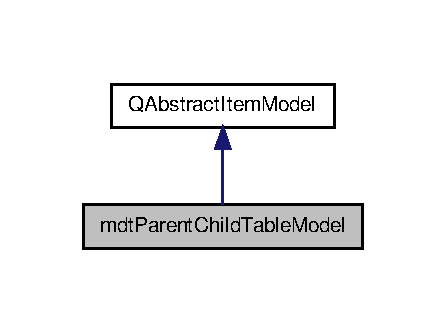
\includegraphics[width=214pt]{classmdt_parent_child_table_model__inherit__graph}
\end{center}
\end{figure}


Collaboration diagram for mdt\-Parent\-Child\-Table\-Model\-:
\nopagebreak
\begin{figure}[H]
\begin{center}
\leavevmode
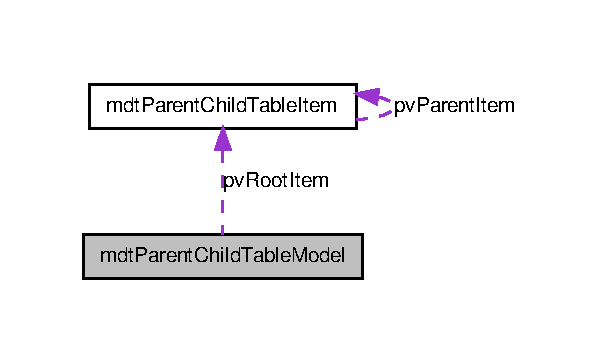
\includegraphics[width=214pt]{classmdt_parent_child_table_model__coll__graph}
\end{center}
\end{figure}
\subsection*{Public Member Functions}
\begin{DoxyCompactItemize}
\item 
\hyperlink{classmdt_parent_child_table_model_a6a02b85f8663bd913b23380381287c0b}{mdt\-Parent\-Child\-Table\-Model} (\hyperlink{class_q_object}{Q\-Object} $\ast$\hyperlink{classmdt_parent_child_table_model_aa4827005e9009f1b0fddf4ae962d6031}{parent}=0)
\item 
\hyperlink{classmdt_parent_child_table_model_abe9a228d3890a3228feeadc14217650e}{$\sim$mdt\-Parent\-Child\-Table\-Model} ()
\item 
int \hyperlink{classmdt_parent_child_table_model_a00ede0aa95a181c04aafffa56bd8f470}{row\-Count} (const Q\-Model\-Index \&\hyperlink{classmdt_parent_child_table_model_aa4827005e9009f1b0fddf4ae962d6031}{parent}=Q\-Model\-Index()) const 
\item 
int \hyperlink{classmdt_parent_child_table_model_a6d1941603fde6be4942439f22616249e}{column\-Count} (const Q\-Model\-Index \&\hyperlink{classmdt_parent_child_table_model_aa4827005e9009f1b0fddf4ae962d6031}{parent}=Q\-Model\-Index()) const 
\item 
Q\-Variant \hyperlink{classmdt_parent_child_table_model_aea9349919cafde88c33aa6ff8c68f4ff}{data} (const Q\-Model\-Index \&\hyperlink{classmdt_parent_child_table_model_abd2bd46910ca92c7b92ff24593bfa4d1}{index}, int role) const 
\item 
void \hyperlink{classmdt_parent_child_table_model_a639b9f817d3c67e913c1e758ceb15f12}{set\-Header\-Data} (Q\-List$<$ Q\-Variant $>$ \&\hyperlink{classmdt_parent_child_table_model_ac0fe230365b4685729886eb89c3bee2d}{header\-Data})
\item 
Q\-Variant \hyperlink{classmdt_parent_child_table_model_ac0fe230365b4685729886eb89c3bee2d}{header\-Data} (int section, Qt\-::\-Orientation orientation, int role=Qt\-::\-Display\-Role) const 
\item 
Qt\-::\-Item\-Flags \hyperlink{classmdt_parent_child_table_model_ad937c815fb4d3afdd7bf6a222e216b2c}{flags} (const Q\-Model\-Index \&\hyperlink{classmdt_parent_child_table_model_abd2bd46910ca92c7b92ff24593bfa4d1}{index}) const 
\item 
Q\-Model\-Index \hyperlink{classmdt_parent_child_table_model_abd2bd46910ca92c7b92ff24593bfa4d1}{index} (int row, int column, const Q\-Model\-Index \&\hyperlink{classmdt_parent_child_table_model_aa4827005e9009f1b0fddf4ae962d6031}{parent}=Q\-Model\-Index()) const 
\item 
Q\-Model\-Index \hyperlink{classmdt_parent_child_table_model_aa4827005e9009f1b0fddf4ae962d6031}{parent} (const Q\-Model\-Index \&\hyperlink{classmdt_parent_child_table_model_abd2bd46910ca92c7b92ff24593bfa4d1}{index}=Q\-Model\-Index()) const 
\end{DoxyCompactItemize}


\subsection{Detailed Description}


Definition at line 12 of file mdt\-Parent\-Child\-Table\-Model.\-h.



\subsection{Constructor \& Destructor Documentation}
\hypertarget{classmdt_parent_child_table_model_a6a02b85f8663bd913b23380381287c0b}{\index{mdt\-Parent\-Child\-Table\-Model@{mdt\-Parent\-Child\-Table\-Model}!mdt\-Parent\-Child\-Table\-Model@{mdt\-Parent\-Child\-Table\-Model}}
\index{mdt\-Parent\-Child\-Table\-Model@{mdt\-Parent\-Child\-Table\-Model}!mdtParentChildTableModel@{mdt\-Parent\-Child\-Table\-Model}}
\subsubsection[{mdt\-Parent\-Child\-Table\-Model}]{\setlength{\rightskip}{0pt plus 5cm}mdt\-Parent\-Child\-Table\-Model\-::mdt\-Parent\-Child\-Table\-Model (
\begin{DoxyParamCaption}
\item[{{\bf Q\-Object} $\ast$}]{parent = {\ttfamily 0}}
\end{DoxyParamCaption}
)}}\label{classmdt_parent_child_table_model_a6a02b85f8663bd913b23380381287c0b}


Definition at line 11 of file mdt\-Parent\-Child\-Table\-Model.\-cpp.

\hypertarget{classmdt_parent_child_table_model_abe9a228d3890a3228feeadc14217650e}{\index{mdt\-Parent\-Child\-Table\-Model@{mdt\-Parent\-Child\-Table\-Model}!$\sim$mdt\-Parent\-Child\-Table\-Model@{$\sim$mdt\-Parent\-Child\-Table\-Model}}
\index{$\sim$mdt\-Parent\-Child\-Table\-Model@{$\sim$mdt\-Parent\-Child\-Table\-Model}!mdtParentChildTableModel@{mdt\-Parent\-Child\-Table\-Model}}
\subsubsection[{$\sim$mdt\-Parent\-Child\-Table\-Model}]{\setlength{\rightskip}{0pt plus 5cm}mdt\-Parent\-Child\-Table\-Model\-::$\sim$mdt\-Parent\-Child\-Table\-Model (
\begin{DoxyParamCaption}
{}
\end{DoxyParamCaption}
)}}\label{classmdt_parent_child_table_model_abe9a228d3890a3228feeadc14217650e}


Definition at line 20 of file mdt\-Parent\-Child\-Table\-Model.\-cpp.



\subsection{Member Function Documentation}
\hypertarget{classmdt_parent_child_table_model_a6d1941603fde6be4942439f22616249e}{\index{mdt\-Parent\-Child\-Table\-Model@{mdt\-Parent\-Child\-Table\-Model}!column\-Count@{column\-Count}}
\index{column\-Count@{column\-Count}!mdtParentChildTableModel@{mdt\-Parent\-Child\-Table\-Model}}
\subsubsection[{column\-Count}]{\setlength{\rightskip}{0pt plus 5cm}int mdt\-Parent\-Child\-Table\-Model\-::column\-Count (
\begin{DoxyParamCaption}
\item[{const Q\-Model\-Index \&}]{parent = {\ttfamily QModelIndex()}}
\end{DoxyParamCaption}
) const}}\label{classmdt_parent_child_table_model_a6d1941603fde6be4942439f22616249e}


Definition at line 42 of file mdt\-Parent\-Child\-Table\-Model.\-cpp.



References mdt\-Parent\-Child\-Table\-Item\-::child(), mdt\-Parent\-Child\-Table\-Item\-::column\-Count(), and mdt\-Parent\-Child\-Table\-Item\-::row().

\hypertarget{classmdt_parent_child_table_model_aea9349919cafde88c33aa6ff8c68f4ff}{\index{mdt\-Parent\-Child\-Table\-Model@{mdt\-Parent\-Child\-Table\-Model}!data@{data}}
\index{data@{data}!mdtParentChildTableModel@{mdt\-Parent\-Child\-Table\-Model}}
\subsubsection[{data}]{\setlength{\rightskip}{0pt plus 5cm}Q\-Variant mdt\-Parent\-Child\-Table\-Model\-::data (
\begin{DoxyParamCaption}
\item[{const Q\-Model\-Index \&}]{index, }
\item[{int}]{role}
\end{DoxyParamCaption}
) const}}\label{classmdt_parent_child_table_model_aea9349919cafde88c33aa6ff8c68f4ff}


Definition at line 61 of file mdt\-Parent\-Child\-Table\-Model.\-cpp.



References mdt\-Parent\-Child\-Table\-Item\-::data().

\hypertarget{classmdt_parent_child_table_model_ad937c815fb4d3afdd7bf6a222e216b2c}{\index{mdt\-Parent\-Child\-Table\-Model@{mdt\-Parent\-Child\-Table\-Model}!flags@{flags}}
\index{flags@{flags}!mdtParentChildTableModel@{mdt\-Parent\-Child\-Table\-Model}}
\subsubsection[{flags}]{\setlength{\rightskip}{0pt plus 5cm}Qt\-::\-Item\-Flags mdt\-Parent\-Child\-Table\-Model\-::flags (
\begin{DoxyParamCaption}
\item[{const Q\-Model\-Index \&}]{index}
\end{DoxyParamCaption}
) const}}\label{classmdt_parent_child_table_model_ad937c815fb4d3afdd7bf6a222e216b2c}


Definition at line 95 of file mdt\-Parent\-Child\-Table\-Model.\-cpp.

\hypertarget{classmdt_parent_child_table_model_ac0fe230365b4685729886eb89c3bee2d}{\index{mdt\-Parent\-Child\-Table\-Model@{mdt\-Parent\-Child\-Table\-Model}!header\-Data@{header\-Data}}
\index{header\-Data@{header\-Data}!mdtParentChildTableModel@{mdt\-Parent\-Child\-Table\-Model}}
\subsubsection[{header\-Data}]{\setlength{\rightskip}{0pt plus 5cm}Q\-Variant mdt\-Parent\-Child\-Table\-Model\-::header\-Data (
\begin{DoxyParamCaption}
\item[{int}]{section, }
\item[{Qt\-::\-Orientation}]{orientation, }
\item[{int}]{role = {\ttfamily Qt\-:\-:DisplayRole}}
\end{DoxyParamCaption}
) const}}\label{classmdt_parent_child_table_model_ac0fe230365b4685729886eb89c3bee2d}


Definition at line 81 of file mdt\-Parent\-Child\-Table\-Model.\-cpp.



Referenced by set\-Header\-Data().

\hypertarget{classmdt_parent_child_table_model_abd2bd46910ca92c7b92ff24593bfa4d1}{\index{mdt\-Parent\-Child\-Table\-Model@{mdt\-Parent\-Child\-Table\-Model}!index@{index}}
\index{index@{index}!mdtParentChildTableModel@{mdt\-Parent\-Child\-Table\-Model}}
\subsubsection[{index}]{\setlength{\rightskip}{0pt plus 5cm}Q\-Model\-Index mdt\-Parent\-Child\-Table\-Model\-::index (
\begin{DoxyParamCaption}
\item[{int}]{row, }
\item[{int}]{column, }
\item[{const Q\-Model\-Index \&}]{parent = {\ttfamily QModelIndex()}}
\end{DoxyParamCaption}
) const}}\label{classmdt_parent_child_table_model_abd2bd46910ca92c7b92ff24593bfa4d1}


Definition at line 104 of file mdt\-Parent\-Child\-Table\-Model.\-cpp.



References mdt\-Parent\-Child\-Table\-Item\-::child().

\hypertarget{classmdt_parent_child_table_model_aa4827005e9009f1b0fddf4ae962d6031}{\index{mdt\-Parent\-Child\-Table\-Model@{mdt\-Parent\-Child\-Table\-Model}!parent@{parent}}
\index{parent@{parent}!mdtParentChildTableModel@{mdt\-Parent\-Child\-Table\-Model}}
\subsubsection[{parent}]{\setlength{\rightskip}{0pt plus 5cm}Q\-Model\-Index mdt\-Parent\-Child\-Table\-Model\-::parent (
\begin{DoxyParamCaption}
\item[{const Q\-Model\-Index \&}]{index = {\ttfamily QModelIndex()}}
\end{DoxyParamCaption}
) const}}\label{classmdt_parent_child_table_model_aa4827005e9009f1b0fddf4ae962d6031}


Definition at line 125 of file mdt\-Parent\-Child\-Table\-Model.\-cpp.



References mdt\-Parent\-Child\-Table\-Item\-::parent(), and mdt\-Parent\-Child\-Table\-Item\-::row().

\hypertarget{classmdt_parent_child_table_model_a00ede0aa95a181c04aafffa56bd8f470}{\index{mdt\-Parent\-Child\-Table\-Model@{mdt\-Parent\-Child\-Table\-Model}!row\-Count@{row\-Count}}
\index{row\-Count@{row\-Count}!mdtParentChildTableModel@{mdt\-Parent\-Child\-Table\-Model}}
\subsubsection[{row\-Count}]{\setlength{\rightskip}{0pt plus 5cm}int mdt\-Parent\-Child\-Table\-Model\-::row\-Count (
\begin{DoxyParamCaption}
\item[{const Q\-Model\-Index \&}]{parent = {\ttfamily QModelIndex()}}
\end{DoxyParamCaption}
) const}}\label{classmdt_parent_child_table_model_a00ede0aa95a181c04aafffa56bd8f470}


Definition at line 25 of file mdt\-Parent\-Child\-Table\-Model.\-cpp.



References mdt\-Parent\-Child\-Table\-Item\-::child\-Count().

\hypertarget{classmdt_parent_child_table_model_a639b9f817d3c67e913c1e758ceb15f12}{\index{mdt\-Parent\-Child\-Table\-Model@{mdt\-Parent\-Child\-Table\-Model}!set\-Header\-Data@{set\-Header\-Data}}
\index{set\-Header\-Data@{set\-Header\-Data}!mdtParentChildTableModel@{mdt\-Parent\-Child\-Table\-Model}}
\subsubsection[{set\-Header\-Data}]{\setlength{\rightskip}{0pt plus 5cm}void mdt\-Parent\-Child\-Table\-Model\-::set\-Header\-Data (
\begin{DoxyParamCaption}
\item[{Q\-List$<$ Q\-Variant $>$ \&}]{header\-Data}
\end{DoxyParamCaption}
)}}\label{classmdt_parent_child_table_model_a639b9f817d3c67e913c1e758ceb15f12}


Definition at line 76 of file mdt\-Parent\-Child\-Table\-Model.\-cpp.



References header\-Data().



The documentation for this class was generated from the following files\-:\begin{DoxyCompactItemize}
\item 
src/mdtutilsgui/\hyperlink{mdt_parent_child_table_model_8h}{mdt\-Parent\-Child\-Table\-Model.\-h}\item 
src/mdtutilsgui/\hyperlink{mdt_parent_child_table_model_8cpp}{mdt\-Parent\-Child\-Table\-Model.\-cpp}\end{DoxyCompactItemize}

\hypertarget{classmdt_port}{
\section{mdtPort Class Reference}
\label{classmdt_port}\index{mdtPort@{mdtPort}}
}


Inheritance diagram for mdtPort:\nopagebreak
\begin{figure}[H]
\begin{center}
\leavevmode
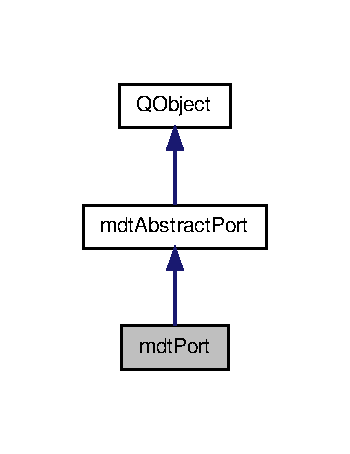
\includegraphics[width=296pt]{classmdt_port__inherit__graph}
\end{center}
\end{figure}
\subsection*{Public Member Functions}
\begin{DoxyCompactItemize}
\item 
\hypertarget{classmdt_port_ac466eac9d1a54ea0e04c998660ad75ec}{
\hyperlink{classmdt_port_ac466eac9d1a54ea0e04c998660ad75ec}{mdtPort} (QObject $\ast$parent=0)}
\label{classmdt_port_ac466eac9d1a54ea0e04c998660ad75ec}

\begin{DoxyCompactList}\small\item\em Construct a new port object R/W timeouts are set to 500 ms. \end{DoxyCompactList}\item 
bool \hyperlink{classmdt_port_ac7158d1d718dbc6068648bbed1eab747}{open} (\hyperlink{classmdt_port_config}{mdtPortConfig} \&cfg)
\begin{DoxyCompactList}\small\item\em Open port. \end{DoxyCompactList}\item 
void \hyperlink{classmdt_port_aa494585a96a16c80a04dd32b0b6a0d4c}{close} ()
\begin{DoxyCompactList}\small\item\em Close the port. \end{DoxyCompactList}\end{DoxyCompactItemize}


\subsection{Member Function Documentation}
\hypertarget{classmdt_port_aa494585a96a16c80a04dd32b0b6a0d4c}{
\index{mdtPort@{mdtPort}!close@{close}}
\index{close@{close}!mdtPort@{mdtPort}}
\subsubsection[{close}]{\setlength{\rightskip}{0pt plus 5cm}void mdtPort::close (
\begin{DoxyParamCaption}
{}
\end{DoxyParamCaption}
)}}
\label{classmdt_port_aa494585a96a16c80a04dd32b0b6a0d4c}


Close the port. 

Note: this method locks the internal mutex 

Reimplemented in \hyperlink{classmdt_serial_port_posix_a29df8d6b7c74bd7e3bf8513987bdd2a2}{mdtSerialPortPosix}, and \hyperlink{classmdt_abstract_serial_port_ad84810a4bd7a10c5c621475511196c85}{mdtAbstractSerialPort}.

\hypertarget{classmdt_port_ac7158d1d718dbc6068648bbed1eab747}{
\index{mdtPort@{mdtPort}!open@{open}}
\index{open@{open}!mdtPort@{mdtPort}}
\subsubsection[{open}]{\setlength{\rightskip}{0pt plus 5cm}bool mdtPort::open (
\begin{DoxyParamCaption}
\item[{{\bf mdtPortConfig} \&}]{cfg}
\end{DoxyParamCaption}
)}}
\label{classmdt_port_ac7158d1d718dbc6068648bbed1eab747}


Open port. 

Note: this method locks the internal mutex 
\begin{DoxyParams}{Parameters}
{\em path} & Path to port \\
\hline
\end{DoxyParams}
\begin{DoxyReturn}{Returns}
True if successfull 
\end{DoxyReturn}


The documentation for this class was generated from the following files:\begin{DoxyCompactItemize}
\item 
src/mdtutils/mdtPort.h\item 
src/mdtutils/mdtPort.cpp\end{DoxyCompactItemize}

\hypertarget{classmdt_port_config}{\section{mdt\-Port\-Config Class Reference}
\label{classmdt_port_config}\index{mdt\-Port\-Config@{mdt\-Port\-Config}}
}


{\ttfamily \#include $<$mdt\-Port\-Config.\-h$>$}



Inheritance diagram for mdt\-Port\-Config\-:\nopagebreak
\begin{figure}[H]
\begin{center}
\leavevmode
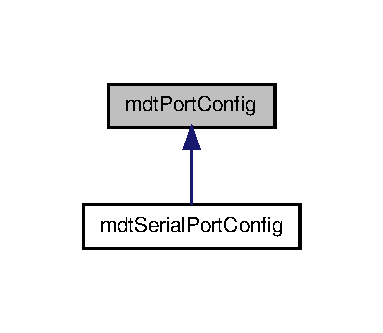
\includegraphics[width=184pt]{classmdt_port_config__inherit__graph}
\end{center}
\end{figure}


Collaboration diagram for mdt\-Port\-Config\-:\nopagebreak
\begin{figure}[H]
\begin{center}
\leavevmode
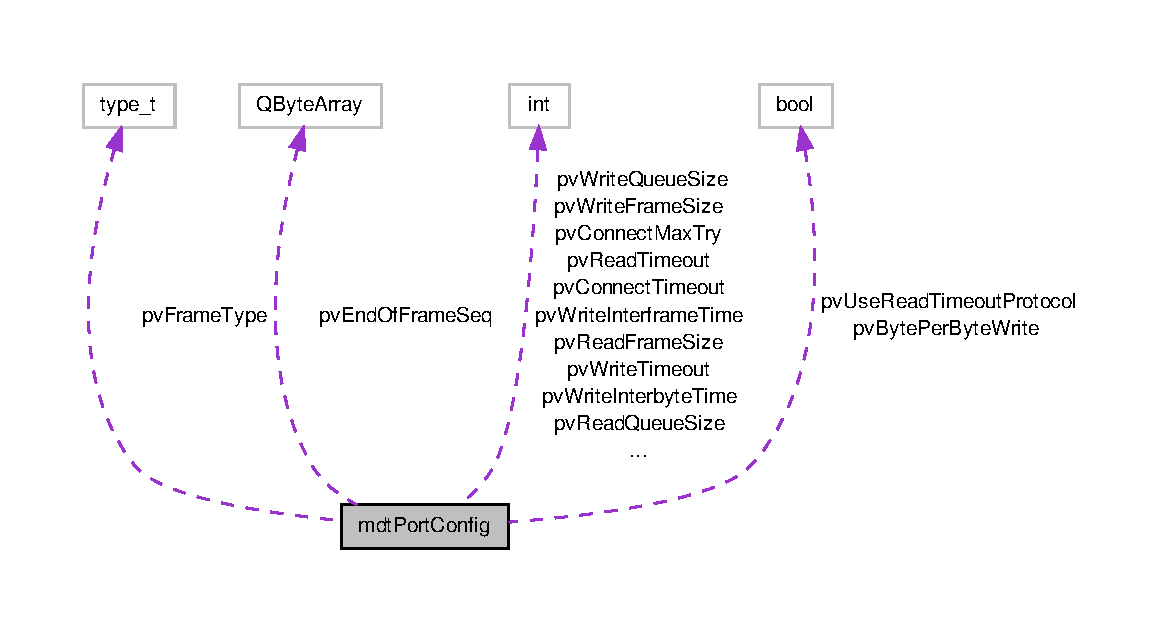
\includegraphics[width=350pt]{classmdt_port_config__coll__graph}
\end{center}
\end{figure}
\subsection*{Public Member Functions}
\begin{DoxyCompactItemize}
\item 
\hyperlink{classmdt_port_config_a7c97a56ca19b074bcfc56672086f8af8}{mdt\-Port\-Config} ()
\item 
virtual \hyperlink{classmdt_port_config_a6dee4709117278c20f9134220770a6cd}{$\sim$mdt\-Port\-Config} ()
\item 
virtual void \hyperlink{classmdt_port_config_a1cad2f21252411977fe328f89b68fbfb}{set\-Default} ()
\begin{DoxyCompactList}\small\item\em Set default configuration. \end{DoxyCompactList}\item 
void \hyperlink{classmdt_port_config_a02f3c9744b0d7a61853ab58467278bbc}{set\-Read\-Frame\-Size} (int size)
\begin{DoxyCompactList}\small\item\em Set the read frame size. \end{DoxyCompactList}\item 
int \hyperlink{classmdt_port_config_ad315f8f97723abe161792c9d9a1375ec}{read\-Frame\-Size} () const 
\begin{DoxyCompactList}\small\item\em Get the read frame size. \end{DoxyCompactList}\item 
void \hyperlink{classmdt_port_config_a04d8e81844deaff20a890ea24e2f9634}{set\-Read\-Queue\-Size} (int size)
\begin{DoxyCompactList}\small\item\em Set the read Queue size. \end{DoxyCompactList}\item 
int \hyperlink{classmdt_port_config_aff0260f72ca05715efe3f70850e7a151}{read\-Queue\-Size} () const 
\begin{DoxyCompactList}\small\item\em Get the read Queue size. \end{DoxyCompactList}\item 
void \hyperlink{classmdt_port_config_a5e7857a56ab2baff4bd0a77290b3c742}{set\-Use\-Read\-Timeout\-Protocol} (bool use)
\begin{DoxyCompactList}\small\item\em Use the read timeout protocol. \end{DoxyCompactList}\item 
bool \hyperlink{classmdt_port_config_ad90a88b06f0efebd1ee9f6d4370dec33}{use\-Read\-Timeout\-Protocol} () const 
\begin{DoxyCompactList}\small\item\em Know if read timeout protocol must be used. \end{DoxyCompactList}\item 
void \hyperlink{classmdt_port_config_a1028f6c9d7073a6591fa59fc907f0585}{set\-Read\-Timeout} (int timeout)
\begin{DoxyCompactList}\small\item\em Set the read timeout. \end{DoxyCompactList}\item 
int \hyperlink{classmdt_port_config_ab18c2ec1628cb480a70033387e7c3333}{read\-Timeout} () const 
\begin{DoxyCompactList}\small\item\em Get read timeout. \end{DoxyCompactList}\item 
void \hyperlink{classmdt_port_config_a7113f6d96e93978cc3915589c14b16b6}{set\-Write\-Interframe\-Time} (int time)
\begin{DoxyCompactList}\small\item\em Set the write interframe time. \end{DoxyCompactList}\item 
int \hyperlink{classmdt_port_config_a745f5111436fc143b75440bf90a1a4e6}{write\-Interframe\-Time} () const 
\begin{DoxyCompactList}\small\item\em Get the write interframe time \mbox{[}ms\mbox{]}. \end{DoxyCompactList}\item 
void \hyperlink{classmdt_port_config_ac117f7cd1f23de163a7fe84f69c2164c}{set\-Write\-Timeout} (int timeout)
\begin{DoxyCompactList}\small\item\em Set the write timeout. \end{DoxyCompactList}\item 
int \hyperlink{classmdt_port_config_a3009e07cd66f4c4bfc1c7fdabbc9f93c}{write\-Timeout} () const 
\begin{DoxyCompactList}\small\item\em Get write timeout. \end{DoxyCompactList}\item 
void \hyperlink{classmdt_port_config_a9539cef9e33d564c7c70902a6380be04}{set\-Write\-Frame\-Size} (int size)
\begin{DoxyCompactList}\small\item\em Set the write frame size. \end{DoxyCompactList}\item 
int \hyperlink{classmdt_port_config_a19bda9f9ce29657179994e02c6da11b9}{write\-Frame\-Size} () const 
\begin{DoxyCompactList}\small\item\em Get the read frame size. \end{DoxyCompactList}\item 
void \hyperlink{classmdt_port_config_a8a99771f7acfeb546d1d89d3671407e5}{set\-Write\-Queue\-Size} (int size)
\begin{DoxyCompactList}\small\item\em Set the read Queue size. \end{DoxyCompactList}\item 
int \hyperlink{classmdt_port_config_a93d72b1ea53f188d7a35bc044394b959}{write\-Queue\-Size} () const 
\begin{DoxyCompactList}\small\item\em Get the write Queue size. \end{DoxyCompactList}\item 
void \hyperlink{classmdt_port_config_a627adcb87d26757238f844db19fc248d}{set\-Frame\-Type} (const \hyperlink{classmdt_frame_af936e37d5fe4c066c0fb0161fafd4a17}{mdt\-Frame\-::type\-\_\-t} type)
\begin{DoxyCompactList}\small\item\em Set frame type. \end{DoxyCompactList}\item 
\hyperlink{classmdt_frame_af936e37d5fe4c066c0fb0161fafd4a17}{mdt\-Frame\-::type\-\_\-t} \hyperlink{classmdt_port_config_af9c95090820c449412298832582a0fab}{frame\-Type} () const 
\begin{DoxyCompactList}\small\item\em Get frame type. \end{DoxyCompactList}\item 
void \hyperlink{classmdt_port_config_a3c5e1c444a18da7d68430bd1c14030f4}{set\-End\-Of\-Frame\-Seq} (const Q\-Byte\-Array \&seq)
\begin{DoxyCompactList}\small\item\em Set the end of frame sequence (applies on A\-S\-C\-I\-I frames) \end{DoxyCompactList}\item 
void \hyperlink{classmdt_port_config_a9c67e95bb660a13313ec03e07a924793}{set\-End\-Of\-Frame\-Seq} (char c)
\begin{DoxyCompactList}\small\item\em Set the end of frame sequence (applies on A\-S\-C\-I\-I frames) \end{DoxyCompactList}\item 
Q\-Byte\-Array \hyperlink{classmdt_port_config_a9ac77f89ee4a0baadc4814a9a95701b6}{end\-Of\-Frame\-Seq} () const 
\begin{DoxyCompactList}\small\item\em Get the end of frame sequence. \end{DoxyCompactList}\item 
void \hyperlink{classmdt_port_config_ac6cb3d8fbefad9a832335c3f2023832c}{set\-Byte\-Per\-Byte\-Write} (bool on, int wait\-Time)
\begin{DoxyCompactList}\small\item\em Set the byte per byte write On/\-Off. \end{DoxyCompactList}\item 
bool \hyperlink{classmdt_port_config_a9b5041ba740a5918e5e1323e61d3bbdc}{byte\-Per\-Byte\-Write} () const 
\begin{DoxyCompactList}\small\item\em Get byte per byte write flag (On/\-Off) \end{DoxyCompactList}\item 
int \hyperlink{classmdt_port_config_a76cc4a35cfd2c762d1f9dacb87203627}{write\-Interbyte\-Time} () const 
\begin{DoxyCompactList}\small\item\em Get the write time between bytes \mbox{[}ms\mbox{]}. \end{DoxyCompactList}\item 
void \hyperlink{classmdt_port_config_a64b8978cc32b97ffe64768fad6f2b0e8}{set\-Connect\-Timeout} (int timeout)
\begin{DoxyCompactList}\small\item\em Set the connection timeout. \end{DoxyCompactList}\item 
int \hyperlink{classmdt_port_config_a1e47b397318c6b4911d40dbbc5c317e7}{connect\-Timeout} () const 
\begin{DoxyCompactList}\small\item\em Get the connection timeout. \end{DoxyCompactList}\item 
void \hyperlink{classmdt_port_config_a1fed4cc77cc33193886e7562369eac88}{set\-Connect\-Max\-Try} (int max\-Try)
\begin{DoxyCompactList}\small\item\em Set the maximum connection try. \end{DoxyCompactList}\item 
int \hyperlink{classmdt_port_config_a98aa42afacba9bfe28d3f02a6b849f60}{connect\-Max\-Try} () const 
\begin{DoxyCompactList}\small\item\em Get the maximum connection try. \end{DoxyCompactList}\item 
bool \hyperlink{classmdt_port_config_a639c71f90cfeb7e2160ad90e9775054b}{operator==} (const \hyperlink{classmdt_port_config}{mdt\-Port\-Config} \&other)
\item 
bool \hyperlink{classmdt_port_config_a5a539c86934d41306a3ed18a8292457d}{operator!=} (const \hyperlink{classmdt_port_config}{mdt\-Port\-Config} \&other)
\end{DoxyCompactItemize}
\subsection*{Protected Member Functions}
\begin{DoxyCompactItemize}
\item 
bool \hyperlink{classmdt_port_config_a6372ebc36d4476899e2274299ae5799d}{matches} (const \hyperlink{classmdt_port_config}{mdt\-Port\-Config} \&other)
\end{DoxyCompactItemize}
\subsection*{Protected Attributes}
\begin{DoxyCompactItemize}
\item 
int \hyperlink{classmdt_port_config_a89f0ded07219e4ddbec5f6f20a3798d5}{pv\-Read\-Frame\-Size}
\item 
int \hyperlink{classmdt_port_config_a999e392fa0d1e97428cef3d45a0f7983}{pv\-Read\-Queue\-Size}
\item 
bool \hyperlink{classmdt_port_config_a1a5ab2cf82ea35db627aa8b87f9dba2e}{pv\-Use\-Read\-Timeout\-Protocol}
\item 
int \hyperlink{classmdt_port_config_a69fa9f6cb32469f3eccfe7517dc29101}{pv\-Read\-Timeout}
\item 
int \hyperlink{classmdt_port_config_aeaeb93ea4d49f66ff9613c7499e670f4}{pv\-Write\-Frame\-Size}
\item 
int \hyperlink{classmdt_port_config_a547f27521b405528f86259fa9aaa37c5}{pv\-Write\-Queue\-Size}
\item 
int \hyperlink{classmdt_port_config_af983cf9d9f9e2f124d6dcc83cdca5a3e}{pv\-Write\-Interbyte\-Time}
\item 
int \hyperlink{classmdt_port_config_ace2001b084ab2611c2de56c951974457}{pv\-Write\-Interframe\-Time}
\item 
int \hyperlink{classmdt_port_config_ad840fd68971a9ccc6092ce2aa3167591}{pv\-Write\-Timeout}
\item 
\hyperlink{classmdt_frame_af936e37d5fe4c066c0fb0161fafd4a17}{mdt\-Frame\-::type\-\_\-t} \hyperlink{classmdt_port_config_a4bc3110b7831ca76954a8d8fc78944f1}{pv\-Frame\-Type}
\item 
Q\-Byte\-Array \hyperlink{classmdt_port_config_ad5d5aeb26cfe98090848a62f5078b22c}{pv\-End\-Of\-Frame\-Seq}
\item 
bool \hyperlink{classmdt_port_config_a56fb67591803bc972772073a6f2b996d}{pv\-Byte\-Per\-Byte\-Write}
\item 
int \hyperlink{classmdt_port_config_a46b87d1b9c2dbe30688497c34807d93c}{pv\-Connect\-Max\-Try}
\item 
int \hyperlink{classmdt_port_config_a3e6aa49486e716f834e174b5ce0a3909}{pv\-Connect\-Timeout}
\end{DoxyCompactItemize}


\subsection{Detailed Description}


Definition at line 28 of file mdt\-Port\-Config.\-h.



\subsection{Constructor \& Destructor Documentation}
\hypertarget{classmdt_port_config_a7c97a56ca19b074bcfc56672086f8af8}{\index{mdt\-Port\-Config@{mdt\-Port\-Config}!mdt\-Port\-Config@{mdt\-Port\-Config}}
\index{mdt\-Port\-Config@{mdt\-Port\-Config}!mdtPortConfig@{mdt\-Port\-Config}}
\subsubsection[{mdt\-Port\-Config}]{\setlength{\rightskip}{0pt plus 5cm}mdt\-Port\-Config\-::mdt\-Port\-Config (
\begin{DoxyParamCaption}
{}
\end{DoxyParamCaption}
)}}\label{classmdt_port_config_a7c97a56ca19b074bcfc56672086f8af8}


Definition at line 23 of file mdt\-Port\-Config.\-cpp.



References set\-Default().

\hypertarget{classmdt_port_config_a6dee4709117278c20f9134220770a6cd}{\index{mdt\-Port\-Config@{mdt\-Port\-Config}!$\sim$mdt\-Port\-Config@{$\sim$mdt\-Port\-Config}}
\index{$\sim$mdt\-Port\-Config@{$\sim$mdt\-Port\-Config}!mdtPortConfig@{mdt\-Port\-Config}}
\subsubsection[{$\sim$mdt\-Port\-Config}]{\setlength{\rightskip}{0pt plus 5cm}mdt\-Port\-Config\-::$\sim$mdt\-Port\-Config (
\begin{DoxyParamCaption}
{}
\end{DoxyParamCaption}
)\hspace{0.3cm}{\ttfamily [virtual]}}}\label{classmdt_port_config_a6dee4709117278c20f9134220770a6cd}


Definition at line 28 of file mdt\-Port\-Config.\-cpp.



\subsection{Member Function Documentation}
\hypertarget{classmdt_port_config_a9b5041ba740a5918e5e1323e61d3bbdc}{\index{mdt\-Port\-Config@{mdt\-Port\-Config}!byte\-Per\-Byte\-Write@{byte\-Per\-Byte\-Write}}
\index{byte\-Per\-Byte\-Write@{byte\-Per\-Byte\-Write}!mdtPortConfig@{mdt\-Port\-Config}}
\subsubsection[{byte\-Per\-Byte\-Write}]{\setlength{\rightskip}{0pt plus 5cm}bool mdt\-Port\-Config\-::byte\-Per\-Byte\-Write (
\begin{DoxyParamCaption}
{}
\end{DoxyParamCaption}
) const}}\label{classmdt_port_config_a9b5041ba740a5918e5e1323e61d3bbdc}


Get byte per byte write flag (On/\-Off) 

\begin{DoxySeeAlso}{See Also}
\hyperlink{classmdt_port_config_ac6cb3d8fbefad9a832335c3f2023832c}{set\-Byte\-Per\-Byte\-Write()} 
\end{DoxySeeAlso}


Definition at line 170 of file mdt\-Port\-Config.\-cpp.



References pv\-Byte\-Per\-Byte\-Write.



Referenced by mdt\-Port\-Config\-Widget\-::display\-Config().

\hypertarget{classmdt_port_config_a98aa42afacba9bfe28d3f02a6b849f60}{\index{mdt\-Port\-Config@{mdt\-Port\-Config}!connect\-Max\-Try@{connect\-Max\-Try}}
\index{connect\-Max\-Try@{connect\-Max\-Try}!mdtPortConfig@{mdt\-Port\-Config}}
\subsubsection[{connect\-Max\-Try}]{\setlength{\rightskip}{0pt plus 5cm}int mdt\-Port\-Config\-::connect\-Max\-Try (
\begin{DoxyParamCaption}
{}
\end{DoxyParamCaption}
) const}}\label{classmdt_port_config_a98aa42afacba9bfe28d3f02a6b849f60}


Get the maximum connection try. 

See \hyperlink{classmdt_port_config_a1fed4cc77cc33193886e7562369eac88}{set\-Connect\-Max\-Try()}. 

Definition at line 195 of file mdt\-Port\-Config.\-cpp.



References pv\-Connect\-Max\-Try.



Referenced by mdt\-Port\-Thread\-Helper\-Socket\-::set\-Socket(), and mdt\-Port\-Thread\-::start().

\hypertarget{classmdt_port_config_a1e47b397318c6b4911d40dbbc5c317e7}{\index{mdt\-Port\-Config@{mdt\-Port\-Config}!connect\-Timeout@{connect\-Timeout}}
\index{connect\-Timeout@{connect\-Timeout}!mdtPortConfig@{mdt\-Port\-Config}}
\subsubsection[{connect\-Timeout}]{\setlength{\rightskip}{0pt plus 5cm}int mdt\-Port\-Config\-::connect\-Timeout (
\begin{DoxyParamCaption}
{}
\end{DoxyParamCaption}
) const}}\label{classmdt_port_config_a1e47b397318c6b4911d40dbbc5c317e7}


Get the connection timeout. 

See \hyperlink{classmdt_port_config_a64b8978cc32b97ffe64768fad6f2b0e8}{set\-Connect\-Timeout()}. 

Definition at line 185 of file mdt\-Port\-Config.\-cpp.



References pv\-Connect\-Timeout.



Referenced by mdt\-Port\-Thread\-Helper\-Socket\-::set\-Socket(), and mdt\-Port\-Thread\-::start().

\hypertarget{classmdt_port_config_a9ac77f89ee4a0baadc4814a9a95701b6}{\index{mdt\-Port\-Config@{mdt\-Port\-Config}!end\-Of\-Frame\-Seq@{end\-Of\-Frame\-Seq}}
\index{end\-Of\-Frame\-Seq@{end\-Of\-Frame\-Seq}!mdtPortConfig@{mdt\-Port\-Config}}
\subsubsection[{end\-Of\-Frame\-Seq}]{\setlength{\rightskip}{0pt plus 5cm}Q\-Byte\-Array mdt\-Port\-Config\-::end\-Of\-Frame\-Seq (
\begin{DoxyParamCaption}
{}
\end{DoxyParamCaption}
) const}}\label{classmdt_port_config_a9ac77f89ee4a0baadc4814a9a95701b6}


Get the end of frame sequence. 

\begin{DoxySeeAlso}{See Also}
\hyperlink{classmdt_port_config_a3c5e1c444a18da7d68430bd1c14030f4}{set\-End\-Of\-Frame\-Seq()} 
\end{DoxySeeAlso}


Definition at line 159 of file mdt\-Port\-Config.\-cpp.



References pv\-End\-Of\-Frame\-Seq.



Referenced by mdt\-Port\-Config\-Widget\-::display\-Config(), and mdt\-Abstract\-Port\-::init\-Queues().

\hypertarget{classmdt_port_config_af9c95090820c449412298832582a0fab}{\index{mdt\-Port\-Config@{mdt\-Port\-Config}!frame\-Type@{frame\-Type}}
\index{frame\-Type@{frame\-Type}!mdtPortConfig@{mdt\-Port\-Config}}
\subsubsection[{frame\-Type}]{\setlength{\rightskip}{0pt plus 5cm}{\bf mdt\-Frame\-::type\-\_\-t} mdt\-Port\-Config\-::frame\-Type (
\begin{DoxyParamCaption}
{}
\end{DoxyParamCaption}
) const}}\label{classmdt_port_config_af9c95090820c449412298832582a0fab}


Get frame type. 

\begin{DoxySeeAlso}{See Also}
\hyperlink{classmdt_port_config_a627adcb87d26757238f844db19fc248d}{set\-Frame\-Type()} 
\end{DoxySeeAlso}


Definition at line 143 of file mdt\-Port\-Config.\-cpp.



References pv\-Frame\-Type.



Referenced by mdt\-Port\-Config\-Widget\-::display\-Config(), mdt\-Abstract\-Port\-::init\-Queues(), and mdt\-Port\-Config\-Widget\-::update\-Config().

\hypertarget{classmdt_port_config_a6372ebc36d4476899e2274299ae5799d}{\index{mdt\-Port\-Config@{mdt\-Port\-Config}!matches@{matches}}
\index{matches@{matches}!mdtPortConfig@{mdt\-Port\-Config}}
\subsubsection[{matches}]{\setlength{\rightskip}{0pt plus 5cm}bool mdt\-Port\-Config\-::matches (
\begin{DoxyParamCaption}
\item[{const {\bf mdt\-Port\-Config} \&}]{other}
\end{DoxyParamCaption}
)\hspace{0.3cm}{\ttfamily [protected]}}}\label{classmdt_port_config_a6372ebc36d4476899e2274299ae5799d}


Definition at line 210 of file mdt\-Port\-Config.\-cpp.



References pv\-Connect\-Max\-Try, pv\-Connect\-Timeout, pv\-End\-Of\-Frame\-Seq, pv\-Frame\-Type, pv\-Read\-Frame\-Size, pv\-Read\-Queue\-Size, pv\-Read\-Timeout, pv\-Write\-Frame\-Size, pv\-Write\-Interbyte\-Time, pv\-Write\-Queue\-Size, and pv\-Write\-Timeout.



Referenced by operator!=(), and operator==().

\hypertarget{classmdt_port_config_a5a539c86934d41306a3ed18a8292457d}{\index{mdt\-Port\-Config@{mdt\-Port\-Config}!operator!=@{operator!=}}
\index{operator!=@{operator!=}!mdtPortConfig@{mdt\-Port\-Config}}
\subsubsection[{operator!=}]{\setlength{\rightskip}{0pt plus 5cm}bool mdt\-Port\-Config\-::operator!= (
\begin{DoxyParamCaption}
\item[{const {\bf mdt\-Port\-Config} \&}]{other}
\end{DoxyParamCaption}
)}}\label{classmdt_port_config_a5a539c86934d41306a3ed18a8292457d}


Definition at line 205 of file mdt\-Port\-Config.\-cpp.



References matches().

\hypertarget{classmdt_port_config_a639c71f90cfeb7e2160ad90e9775054b}{\index{mdt\-Port\-Config@{mdt\-Port\-Config}!operator==@{operator==}}
\index{operator==@{operator==}!mdtPortConfig@{mdt\-Port\-Config}}
\subsubsection[{operator==}]{\setlength{\rightskip}{0pt plus 5cm}bool mdt\-Port\-Config\-::operator== (
\begin{DoxyParamCaption}
\item[{const {\bf mdt\-Port\-Config} \&}]{other}
\end{DoxyParamCaption}
)}}\label{classmdt_port_config_a639c71f90cfeb7e2160ad90e9775054b}


Definition at line 200 of file mdt\-Port\-Config.\-cpp.



References matches().

\hypertarget{classmdt_port_config_ad315f8f97723abe161792c9d9a1375ec}{\index{mdt\-Port\-Config@{mdt\-Port\-Config}!read\-Frame\-Size@{read\-Frame\-Size}}
\index{read\-Frame\-Size@{read\-Frame\-Size}!mdtPortConfig@{mdt\-Port\-Config}}
\subsubsection[{read\-Frame\-Size}]{\setlength{\rightskip}{0pt plus 5cm}int mdt\-Port\-Config\-::read\-Frame\-Size (
\begin{DoxyParamCaption}
{}
\end{DoxyParamCaption}
) const}}\label{classmdt_port_config_ad315f8f97723abe161792c9d9a1375ec}


Get the read frame size. 

\begin{DoxySeeAlso}{See Also}
\hyperlink{classmdt_port_config_a02f3c9744b0d7a61853ab58467278bbc}{set\-Read\-Frame\-Size()} 
\end{DoxySeeAlso}


Definition at line 57 of file mdt\-Port\-Config.\-cpp.



References pv\-Read\-Frame\-Size.



Referenced by mdt\-Port\-Config\-Widget\-::display\-Config().

\hypertarget{classmdt_port_config_aff0260f72ca05715efe3f70850e7a151}{\index{mdt\-Port\-Config@{mdt\-Port\-Config}!read\-Queue\-Size@{read\-Queue\-Size}}
\index{read\-Queue\-Size@{read\-Queue\-Size}!mdtPortConfig@{mdt\-Port\-Config}}
\subsubsection[{read\-Queue\-Size}]{\setlength{\rightskip}{0pt plus 5cm}int mdt\-Port\-Config\-::read\-Queue\-Size (
\begin{DoxyParamCaption}
{}
\end{DoxyParamCaption}
) const}}\label{classmdt_port_config_aff0260f72ca05715efe3f70850e7a151}


Get the read Queue size. 

\begin{DoxySeeAlso}{See Also}
\hyperlink{classmdt_port_config_a04d8e81844deaff20a890ea24e2f9634}{set\-Read\-Queue\-Size()} 
\end{DoxySeeAlso}


Definition at line 69 of file mdt\-Port\-Config.\-cpp.



References pv\-Read\-Queue\-Size.



Referenced by mdt\-Port\-Config\-Widget\-::display\-Config(), and mdt\-Abstract\-Port\-::init\-Queues().

\hypertarget{classmdt_port_config_ab18c2ec1628cb480a70033387e7c3333}{\index{mdt\-Port\-Config@{mdt\-Port\-Config}!read\-Timeout@{read\-Timeout}}
\index{read\-Timeout@{read\-Timeout}!mdtPortConfig@{mdt\-Port\-Config}}
\subsubsection[{read\-Timeout}]{\setlength{\rightskip}{0pt plus 5cm}int mdt\-Port\-Config\-::read\-Timeout (
\begin{DoxyParamCaption}
{}
\end{DoxyParamCaption}
) const}}\label{classmdt_port_config_ab18c2ec1628cb480a70033387e7c3333}


Get read timeout. 

\begin{DoxyReturn}{Returns}
Read timout \mbox{[}ms\mbox{]} 
\end{DoxyReturn}


Definition at line 89 of file mdt\-Port\-Config.\-cpp.



References pv\-Read\-Timeout.



Referenced by mdt\-Port\-Config\-Widget\-::display\-Config(), mdt\-Device\-Modbus\-::mdt\-Device\-Modbus(), mdt\-Device\-Scpi\-::mdt\-Device\-Scpi(), mdt\-Port\-Thread\-Helper\-Socket\-::set\-Socket(), and mdt\-Abstract\-Port\-::wait\-For\-Ready\-Read().

\hypertarget{classmdt_port_config_ac6cb3d8fbefad9a832335c3f2023832c}{\index{mdt\-Port\-Config@{mdt\-Port\-Config}!set\-Byte\-Per\-Byte\-Write@{set\-Byte\-Per\-Byte\-Write}}
\index{set\-Byte\-Per\-Byte\-Write@{set\-Byte\-Per\-Byte\-Write}!mdtPortConfig@{mdt\-Port\-Config}}
\subsubsection[{set\-Byte\-Per\-Byte\-Write}]{\setlength{\rightskip}{0pt plus 5cm}void mdt\-Port\-Config\-::set\-Byte\-Per\-Byte\-Write (
\begin{DoxyParamCaption}
\item[{bool}]{on, }
\item[{int}]{wait\-Time}
\end{DoxyParamCaption}
)}}\label{classmdt_port_config_ac6cb3d8fbefad9a832335c3f2023832c}


Set the byte per byte write On/\-Off. 

It can happen that a (very) slow device needs time after any received byte.

Enable this function in this situation.


\begin{DoxyParams}{Parameters}
{\em on} & True will enable this mode. \\
\hline
{\em wait\-Time} & Wait time between two bytes write \mbox{[}ms\mbox{]} \\
\hline
\end{DoxyParams}
\begin{DoxySeeAlso}{See Also}
\hyperlink{classmdt_port_write_thread}{mdt\-Port\-Write\-Thread} 
\end{DoxySeeAlso}


Definition at line 164 of file mdt\-Port\-Config.\-cpp.



References pv\-Byte\-Per\-Byte\-Write, and pv\-Write\-Interbyte\-Time.



Referenced by mdt\-Port\-Config\-Widget\-::update\-Config().

\hypertarget{classmdt_port_config_a1fed4cc77cc33193886e7562369eac88}{\index{mdt\-Port\-Config@{mdt\-Port\-Config}!set\-Connect\-Max\-Try@{set\-Connect\-Max\-Try}}
\index{set\-Connect\-Max\-Try@{set\-Connect\-Max\-Try}!mdtPortConfig@{mdt\-Port\-Config}}
\subsubsection[{set\-Connect\-Max\-Try}]{\setlength{\rightskip}{0pt plus 5cm}void mdt\-Port\-Config\-::set\-Connect\-Max\-Try (
\begin{DoxyParamCaption}
\item[{int}]{max\-Try}
\end{DoxyParamCaption}
)}}\label{classmdt_port_config_a1fed4cc77cc33193886e7562369eac88}


Set the maximum connection try. 

This is used by port witch support disconnection (U\-S\-B, T\-C\-P socket) 

Definition at line 190 of file mdt\-Port\-Config.\-cpp.



References pv\-Connect\-Max\-Try.

\hypertarget{classmdt_port_config_a64b8978cc32b97ffe64768fad6f2b0e8}{\index{mdt\-Port\-Config@{mdt\-Port\-Config}!set\-Connect\-Timeout@{set\-Connect\-Timeout}}
\index{set\-Connect\-Timeout@{set\-Connect\-Timeout}!mdtPortConfig@{mdt\-Port\-Config}}
\subsubsection[{set\-Connect\-Timeout}]{\setlength{\rightskip}{0pt plus 5cm}void mdt\-Port\-Config\-::set\-Connect\-Timeout (
\begin{DoxyParamCaption}
\item[{int}]{timeout}
\end{DoxyParamCaption}
)}}\label{classmdt_port_config_a64b8978cc32b97ffe64768fad6f2b0e8}


Set the connection timeout. 


\begin{DoxyParams}{Parameters}
{\em timeout} & \mbox{[}ms\mbox{]}\\
\hline
\end{DoxyParams}
This is used by port witch support disconnection (U\-S\-B, T\-C\-P socket) 

Definition at line 180 of file mdt\-Port\-Config.\-cpp.



References pv\-Connect\-Timeout.

\hypertarget{classmdt_port_config_a1cad2f21252411977fe328f89b68fbfb}{\index{mdt\-Port\-Config@{mdt\-Port\-Config}!set\-Default@{set\-Default}}
\index{set\-Default@{set\-Default}!mdtPortConfig@{mdt\-Port\-Config}}
\subsubsection[{set\-Default}]{\setlength{\rightskip}{0pt plus 5cm}void mdt\-Port\-Config\-::set\-Default (
\begin{DoxyParamCaption}
{}
\end{DoxyParamCaption}
)\hspace{0.3cm}{\ttfamily [virtual]}}}\label{classmdt_port_config_a1cad2f21252411977fe328f89b68fbfb}


Set default configuration. 

Default configuration is\-:
\begin{DoxyItemize}
\item Read and write frame size\-: 1024
\item Read and write queue size\-: 10
\item Use read timeout protocol\-: false
\item Read timout\-: 5000 \mbox{[}ms\mbox{]}
\item Write timout\-: -\/1 (infinite)
\item Frame type\-: R\-A\-W
\item En of frame sequence\-: L\-F (A\-S\-C\-I\-I 0x0\-A)
\item Write interframe time\-: 0 \mbox{[}ms\mbox{]}
\item Byte per byte write\-: Off
\item Write interbyte time\-: 0 \mbox{[}ms\mbox{]}
\item Connect timeout\-: 5000 \mbox{[}ms\mbox{]}
\item Connect max try\-: 10 
\end{DoxyItemize}

Reimplemented in \hyperlink{classmdt_serial_port_config_acabcdbda285314992582e5ffd413b555}{mdt\-Serial\-Port\-Config}.



Definition at line 31 of file mdt\-Port\-Config.\-cpp.



References mdt\-Frame\-::\-F\-T\-\_\-\-R\-A\-W, pv\-Byte\-Per\-Byte\-Write, pv\-Connect\-Max\-Try, pv\-Connect\-Timeout, pv\-End\-Of\-Frame\-Seq, pv\-Frame\-Type, pv\-Read\-Frame\-Size, pv\-Read\-Queue\-Size, pv\-Read\-Timeout, pv\-Use\-Read\-Timeout\-Protocol, pv\-Write\-Frame\-Size, pv\-Write\-Interbyte\-Time, pv\-Write\-Interframe\-Time, pv\-Write\-Queue\-Size, and pv\-Write\-Timeout.



Referenced by mdt\-Port\-Config(), and mdt\-Serial\-Port\-Config\-::set\-Default().

\hypertarget{classmdt_port_config_a3c5e1c444a18da7d68430bd1c14030f4}{\index{mdt\-Port\-Config@{mdt\-Port\-Config}!set\-End\-Of\-Frame\-Seq@{set\-End\-Of\-Frame\-Seq}}
\index{set\-End\-Of\-Frame\-Seq@{set\-End\-Of\-Frame\-Seq}!mdtPortConfig@{mdt\-Port\-Config}}
\subsubsection[{set\-End\-Of\-Frame\-Seq}]{\setlength{\rightskip}{0pt plus 5cm}void mdt\-Port\-Config\-::set\-End\-Of\-Frame\-Seq (
\begin{DoxyParamCaption}
\item[{const Q\-Byte\-Array \&}]{seq}
\end{DoxyParamCaption}
)}}\label{classmdt_port_config_a3c5e1c444a18da7d68430bd1c14030f4}


Set the end of frame sequence (applies on A\-S\-C\-I\-I frames) 



Definition at line 148 of file mdt\-Port\-Config.\-cpp.



References pv\-End\-Of\-Frame\-Seq.



Referenced by mdt\-Port\-Config\-Widget\-::update\-Config().

\hypertarget{classmdt_port_config_a9c67e95bb660a13313ec03e07a924793}{\index{mdt\-Port\-Config@{mdt\-Port\-Config}!set\-End\-Of\-Frame\-Seq@{set\-End\-Of\-Frame\-Seq}}
\index{set\-End\-Of\-Frame\-Seq@{set\-End\-Of\-Frame\-Seq}!mdtPortConfig@{mdt\-Port\-Config}}
\subsubsection[{set\-End\-Of\-Frame\-Seq}]{\setlength{\rightskip}{0pt plus 5cm}void mdt\-Port\-Config\-::set\-End\-Of\-Frame\-Seq (
\begin{DoxyParamCaption}
\item[{char}]{c}
\end{DoxyParamCaption}
)}}\label{classmdt_port_config_a9c67e95bb660a13313ec03e07a924793}


Set the end of frame sequence (applies on A\-S\-C\-I\-I frames) 

This is an overloaded method

\begin{DoxySeeAlso}{See Also}
\hyperlink{classmdt_port_config_a3c5e1c444a18da7d68430bd1c14030f4}{set\-End\-Of\-Frame\-Seq(const Q\-Byte\-Array \&)} 
\end{DoxySeeAlso}


Definition at line 153 of file mdt\-Port\-Config.\-cpp.



References pv\-End\-Of\-Frame\-Seq.

\hypertarget{classmdt_port_config_a627adcb87d26757238f844db19fc248d}{\index{mdt\-Port\-Config@{mdt\-Port\-Config}!set\-Frame\-Type@{set\-Frame\-Type}}
\index{set\-Frame\-Type@{set\-Frame\-Type}!mdtPortConfig@{mdt\-Port\-Config}}
\subsubsection[{set\-Frame\-Type}]{\setlength{\rightskip}{0pt plus 5cm}void mdt\-Port\-Config\-::set\-Frame\-Type (
\begin{DoxyParamCaption}
\item[{const {\bf mdt\-Frame\-::type\-\_\-t}}]{type}
\end{DoxyParamCaption}
)}}\label{classmdt_port_config_a627adcb87d26757238f844db19fc248d}


Set frame type. 

Frame type can be an A\-S\-C\-I\-I frame, binary frame, ...

\begin{DoxySeeAlso}{See Also}
\hyperlink{classmdt_frame}{mdt\-Frame} 
\end{DoxySeeAlso}


Definition at line 138 of file mdt\-Port\-Config.\-cpp.



References pv\-Frame\-Type.



Referenced by mdt\-Modbus\-Tcp\-Port\-Manager\-::mdt\-Modbus\-Tcp\-Port\-Manager(), mdt\-Usbtmc\-Port\-Manager\-::mdt\-Usbtmc\-Port\-Manager(), and mdt\-Port\-Config\-Widget\-::update\-Config().

\hypertarget{classmdt_port_config_a02f3c9744b0d7a61853ab58467278bbc}{\index{mdt\-Port\-Config@{mdt\-Port\-Config}!set\-Read\-Frame\-Size@{set\-Read\-Frame\-Size}}
\index{set\-Read\-Frame\-Size@{set\-Read\-Frame\-Size}!mdtPortConfig@{mdt\-Port\-Config}}
\subsubsection[{set\-Read\-Frame\-Size}]{\setlength{\rightskip}{0pt plus 5cm}void mdt\-Port\-Config\-::set\-Read\-Frame\-Size (
\begin{DoxyParamCaption}
\item[{int}]{size}
\end{DoxyParamCaption}
)}}\label{classmdt_port_config_a02f3c9744b0d7a61853ab58467278bbc}


Set the read frame size. 

Frame size is the maximum number of bytes that can be stored before a frame is full. A full frame that never received a E\-O\-F condition is considered invalid \begin{DoxySeeAlso}{See Also}
\hyperlink{classmdt_frame}{mdt\-Frame} 
\end{DoxySeeAlso}
\begin{DoxyPrecond}{Precondition}
size must be a positive value 
\end{DoxyPrecond}


Definition at line 50 of file mdt\-Port\-Config.\-cpp.



References pv\-Read\-Frame\-Size.



Referenced by mdt\-Device\-D\-S\-O1000\-A\-::mdt\-Device\-D\-S\-O1000\-A(), mdt\-Device\-U3606\-A\-::mdt\-Device\-U3606\-A(), mdt\-Modbus\-Tcp\-Port\-Manager\-::mdt\-Modbus\-Tcp\-Port\-Manager(), and mdt\-Port\-Config\-Widget\-::update\-Config().

\hypertarget{classmdt_port_config_a04d8e81844deaff20a890ea24e2f9634}{\index{mdt\-Port\-Config@{mdt\-Port\-Config}!set\-Read\-Queue\-Size@{set\-Read\-Queue\-Size}}
\index{set\-Read\-Queue\-Size@{set\-Read\-Queue\-Size}!mdtPortConfig@{mdt\-Port\-Config}}
\subsubsection[{set\-Read\-Queue\-Size}]{\setlength{\rightskip}{0pt plus 5cm}void mdt\-Port\-Config\-::set\-Read\-Queue\-Size (
\begin{DoxyParamCaption}
\item[{int}]{size}
\end{DoxyParamCaption}
)}}\label{classmdt_port_config_a04d8e81844deaff20a890ea24e2f9634}


Set the read Queue size. 

A queue contain several frames. This parameter gives a limit of the number of frame that can be received before they are threated \begin{DoxyPrecond}{Precondition}
size must be a positive value 
\end{DoxyPrecond}


Definition at line 62 of file mdt\-Port\-Config.\-cpp.



References pv\-Read\-Queue\-Size.



Referenced by mdt\-Device\-D\-S\-O1000\-A\-::mdt\-Device\-D\-S\-O1000\-A(), mdt\-Device\-U3606\-A\-::mdt\-Device\-U3606\-A(), and mdt\-Port\-Config\-Widget\-::update\-Config().

\hypertarget{classmdt_port_config_a1028f6c9d7073a6591fa59fc907f0585}{\index{mdt\-Port\-Config@{mdt\-Port\-Config}!set\-Read\-Timeout@{set\-Read\-Timeout}}
\index{set\-Read\-Timeout@{set\-Read\-Timeout}!mdtPortConfig@{mdt\-Port\-Config}}
\subsubsection[{set\-Read\-Timeout}]{\setlength{\rightskip}{0pt plus 5cm}void mdt\-Port\-Config\-::set\-Read\-Timeout (
\begin{DoxyParamCaption}
\item[{int}]{timeout}
\end{DoxyParamCaption}
)}}\label{classmdt_port_config_a1028f6c9d7073a6591fa59fc907f0585}


Set the read timeout. 


\begin{DoxyParams}{Parameters}
{\em timeout} & Read timout \mbox{[}ms\mbox{]} \\
\hline
\end{DoxyParams}


Definition at line 84 of file mdt\-Port\-Config.\-cpp.



References pv\-Read\-Timeout.



Referenced by mdt\-Device\-D\-S\-O1000\-A\-::mdt\-Device\-D\-S\-O1000\-A(), mdt\-Device\-Scpi\-::mdt\-Device\-Scpi(), mdt\-Device\-U3606\-A\-::mdt\-Device\-U3606\-A(), mdt\-Modbus\-Tcp\-Port\-Manager\-::mdt\-Modbus\-Tcp\-Port\-Manager(), mdt\-Usbtmc\-Port\-Manager\-::mdt\-Usbtmc\-Port\-Manager(), and mdt\-Port\-Config\-Widget\-::update\-Config().

\hypertarget{classmdt_port_config_a5e7857a56ab2baff4bd0a77290b3c742}{\index{mdt\-Port\-Config@{mdt\-Port\-Config}!set\-Use\-Read\-Timeout\-Protocol@{set\-Use\-Read\-Timeout\-Protocol}}
\index{set\-Use\-Read\-Timeout\-Protocol@{set\-Use\-Read\-Timeout\-Protocol}!mdtPortConfig@{mdt\-Port\-Config}}
\subsubsection[{set\-Use\-Read\-Timeout\-Protocol}]{\setlength{\rightskip}{0pt plus 5cm}void mdt\-Port\-Config\-::set\-Use\-Read\-Timeout\-Protocol (
\begin{DoxyParamCaption}
\item[{bool}]{use}
\end{DoxyParamCaption}
)}}\label{classmdt_port_config_a5e7857a56ab2baff4bd0a77290b3c742}


Use the read timeout protocol. 

An example of read timeout protocol is M\-O\-D\-B\-U\-S (over serial lines) R\-T\-U mode The \hyperlink{classmdt_port_read_thread}{mdt\-Port\-Read\-Thread} will use this parameter.


\begin{DoxyParams}{Parameters}
{\em use} & If true, read timeout protocol will be used. \\
\hline
\end{DoxyParams}


Definition at line 74 of file mdt\-Port\-Config.\-cpp.



References pv\-Use\-Read\-Timeout\-Protocol.



Referenced by mdt\-Port\-Config\-Widget\-::update\-Config().

\hypertarget{classmdt_port_config_a9539cef9e33d564c7c70902a6380be04}{\index{mdt\-Port\-Config@{mdt\-Port\-Config}!set\-Write\-Frame\-Size@{set\-Write\-Frame\-Size}}
\index{set\-Write\-Frame\-Size@{set\-Write\-Frame\-Size}!mdtPortConfig@{mdt\-Port\-Config}}
\subsubsection[{set\-Write\-Frame\-Size}]{\setlength{\rightskip}{0pt plus 5cm}void mdt\-Port\-Config\-::set\-Write\-Frame\-Size (
\begin{DoxyParamCaption}
\item[{int}]{size}
\end{DoxyParamCaption}
)}}\label{classmdt_port_config_a9539cef9e33d564c7c70902a6380be04}


Set the write frame size. 

Frame size is the maximum number of bytes that can be stored before a frame is full.

\begin{DoxySeeAlso}{See Also}
\hyperlink{classmdt_frame}{mdt\-Frame} 
\end{DoxySeeAlso}
\begin{DoxyPrecond}{Precondition}
size must be a positive value 
\end{DoxyPrecond}


Definition at line 114 of file mdt\-Port\-Config.\-cpp.



References pv\-Write\-Frame\-Size.



Referenced by mdt\-Device\-D\-S\-O1000\-A\-::mdt\-Device\-D\-S\-O1000\-A(), mdt\-Device\-U3606\-A\-::mdt\-Device\-U3606\-A(), mdt\-Modbus\-Tcp\-Port\-Manager\-::mdt\-Modbus\-Tcp\-Port\-Manager(), and mdt\-Port\-Config\-Widget\-::update\-Config().

\hypertarget{classmdt_port_config_a7113f6d96e93978cc3915589c14b16b6}{\index{mdt\-Port\-Config@{mdt\-Port\-Config}!set\-Write\-Interframe\-Time@{set\-Write\-Interframe\-Time}}
\index{set\-Write\-Interframe\-Time@{set\-Write\-Interframe\-Time}!mdtPortConfig@{mdt\-Port\-Config}}
\subsubsection[{set\-Write\-Interframe\-Time}]{\setlength{\rightskip}{0pt plus 5cm}void mdt\-Port\-Config\-::set\-Write\-Interframe\-Time (
\begin{DoxyParamCaption}
\item[{int}]{time}
\end{DoxyParamCaption}
)}}\label{classmdt_port_config_a7113f6d96e93978cc3915589c14b16b6}


Set the write interframe time. 

If this time is $>$ 0 , the \hyperlink{classmdt_port_write_thread}{mdt\-Port\-Write\-Thread} will wait defined time before sending a new frame. This is usefull in timeout based protocols, like Modbus R\-T\-U.


\begin{DoxyParams}{Parameters}
{\em time} & Interframe time \mbox{[}ms\mbox{]} \\
\hline
\end{DoxyParams}


Definition at line 94 of file mdt\-Port\-Config.\-cpp.



References pv\-Write\-Interframe\-Time.



Referenced by mdt\-Port\-Config\-Widget\-::update\-Config().

\hypertarget{classmdt_port_config_a8a99771f7acfeb546d1d89d3671407e5}{\index{mdt\-Port\-Config@{mdt\-Port\-Config}!set\-Write\-Queue\-Size@{set\-Write\-Queue\-Size}}
\index{set\-Write\-Queue\-Size@{set\-Write\-Queue\-Size}!mdtPortConfig@{mdt\-Port\-Config}}
\subsubsection[{set\-Write\-Queue\-Size}]{\setlength{\rightskip}{0pt plus 5cm}void mdt\-Port\-Config\-::set\-Write\-Queue\-Size (
\begin{DoxyParamCaption}
\item[{int}]{size}
\end{DoxyParamCaption}
)}}\label{classmdt_port_config_a8a99771f7acfeb546d1d89d3671407e5}


Set the read Queue size. 

A queue contain several frames. This parameter gives a limit of the number of frame that can be enqueued to serial port output.

\begin{DoxyPrecond}{Precondition}
size must be a positive value 
\end{DoxyPrecond}


Definition at line 126 of file mdt\-Port\-Config.\-cpp.



References pv\-Write\-Queue\-Size.



Referenced by mdt\-Device\-D\-S\-O1000\-A\-::mdt\-Device\-D\-S\-O1000\-A(), mdt\-Device\-U3606\-A\-::mdt\-Device\-U3606\-A(), mdt\-Modbus\-Tcp\-Port\-Manager\-::mdt\-Modbus\-Tcp\-Port\-Manager(), and mdt\-Port\-Config\-Widget\-::update\-Config().

\hypertarget{classmdt_port_config_ac117f7cd1f23de163a7fe84f69c2164c}{\index{mdt\-Port\-Config@{mdt\-Port\-Config}!set\-Write\-Timeout@{set\-Write\-Timeout}}
\index{set\-Write\-Timeout@{set\-Write\-Timeout}!mdtPortConfig@{mdt\-Port\-Config}}
\subsubsection[{set\-Write\-Timeout}]{\setlength{\rightskip}{0pt plus 5cm}void mdt\-Port\-Config\-::set\-Write\-Timeout (
\begin{DoxyParamCaption}
\item[{int}]{timeout}
\end{DoxyParamCaption}
)}}\label{classmdt_port_config_ac117f7cd1f23de163a7fe84f69c2164c}


Set the write timeout. 


\begin{DoxyParams}{Parameters}
{\em timeout} & Write timout \mbox{[}ms\mbox{]} \\
\hline
\end{DoxyParams}


Definition at line 104 of file mdt\-Port\-Config.\-cpp.



References pv\-Write\-Timeout.



Referenced by mdt\-Port\-Config\-Widget\-::update\-Config().

\hypertarget{classmdt_port_config_ad90a88b06f0efebd1ee9f6d4370dec33}{\index{mdt\-Port\-Config@{mdt\-Port\-Config}!use\-Read\-Timeout\-Protocol@{use\-Read\-Timeout\-Protocol}}
\index{use\-Read\-Timeout\-Protocol@{use\-Read\-Timeout\-Protocol}!mdtPortConfig@{mdt\-Port\-Config}}
\subsubsection[{use\-Read\-Timeout\-Protocol}]{\setlength{\rightskip}{0pt plus 5cm}bool mdt\-Port\-Config\-::use\-Read\-Timeout\-Protocol (
\begin{DoxyParamCaption}
{}
\end{DoxyParamCaption}
) const}}\label{classmdt_port_config_ad90a88b06f0efebd1ee9f6d4370dec33}


Know if read timeout protocol must be used. 

\begin{DoxySeeAlso}{See Also}
\hyperlink{classmdt_port_config_a5e7857a56ab2baff4bd0a77290b3c742}{set\-Use\-Read\-Timeout\-Protocol()} 
\end{DoxySeeAlso}


Definition at line 79 of file mdt\-Port\-Config.\-cpp.



References pv\-Use\-Read\-Timeout\-Protocol.



Referenced by mdt\-Port\-Config\-Widget\-::display\-Config().

\hypertarget{classmdt_port_config_a19bda9f9ce29657179994e02c6da11b9}{\index{mdt\-Port\-Config@{mdt\-Port\-Config}!write\-Frame\-Size@{write\-Frame\-Size}}
\index{write\-Frame\-Size@{write\-Frame\-Size}!mdtPortConfig@{mdt\-Port\-Config}}
\subsubsection[{write\-Frame\-Size}]{\setlength{\rightskip}{0pt plus 5cm}int mdt\-Port\-Config\-::write\-Frame\-Size (
\begin{DoxyParamCaption}
{}
\end{DoxyParamCaption}
) const}}\label{classmdt_port_config_a19bda9f9ce29657179994e02c6da11b9}


Get the read frame size. 

\begin{DoxySeeAlso}{See Also}
\hyperlink{classmdt_port_config_a9539cef9e33d564c7c70902a6380be04}{set\-Write\-Frame\-Size()} 
\end{DoxySeeAlso}


Definition at line 121 of file mdt\-Port\-Config.\-cpp.



References pv\-Write\-Frame\-Size.



Referenced by mdt\-Port\-Config\-Widget\-::display\-Config().

\hypertarget{classmdt_port_config_a76cc4a35cfd2c762d1f9dacb87203627}{\index{mdt\-Port\-Config@{mdt\-Port\-Config}!write\-Interbyte\-Time@{write\-Interbyte\-Time}}
\index{write\-Interbyte\-Time@{write\-Interbyte\-Time}!mdtPortConfig@{mdt\-Port\-Config}}
\subsubsection[{write\-Interbyte\-Time}]{\setlength{\rightskip}{0pt plus 5cm}int mdt\-Port\-Config\-::write\-Interbyte\-Time (
\begin{DoxyParamCaption}
{}
\end{DoxyParamCaption}
) const}}\label{classmdt_port_config_a76cc4a35cfd2c762d1f9dacb87203627}


Get the write time between bytes \mbox{[}ms\mbox{]}. 

\begin{DoxySeeAlso}{See Also}
\hyperlink{classmdt_port_config_ac6cb3d8fbefad9a832335c3f2023832c}{set\-Byte\-Per\-Byte\-Write()} 
\end{DoxySeeAlso}


Definition at line 175 of file mdt\-Port\-Config.\-cpp.



References pv\-Write\-Interbyte\-Time.



Referenced by mdt\-Port\-Config\-Widget\-::display\-Config().

\hypertarget{classmdt_port_config_a745f5111436fc143b75440bf90a1a4e6}{\index{mdt\-Port\-Config@{mdt\-Port\-Config}!write\-Interframe\-Time@{write\-Interframe\-Time}}
\index{write\-Interframe\-Time@{write\-Interframe\-Time}!mdtPortConfig@{mdt\-Port\-Config}}
\subsubsection[{write\-Interframe\-Time}]{\setlength{\rightskip}{0pt plus 5cm}int mdt\-Port\-Config\-::write\-Interframe\-Time (
\begin{DoxyParamCaption}
{}
\end{DoxyParamCaption}
) const}}\label{classmdt_port_config_a745f5111436fc143b75440bf90a1a4e6}


Get the write interframe time \mbox{[}ms\mbox{]}. 

\begin{DoxySeeAlso}{See Also}
\hyperlink{classmdt_port_config_a7113f6d96e93978cc3915589c14b16b6}{set\-Write\-Interframe\-Time()} 
\end{DoxySeeAlso}


Definition at line 99 of file mdt\-Port\-Config.\-cpp.



References pv\-Write\-Interframe\-Time.



Referenced by mdt\-Port\-Config\-Widget\-::display\-Config().

\hypertarget{classmdt_port_config_a93d72b1ea53f188d7a35bc044394b959}{\index{mdt\-Port\-Config@{mdt\-Port\-Config}!write\-Queue\-Size@{write\-Queue\-Size}}
\index{write\-Queue\-Size@{write\-Queue\-Size}!mdtPortConfig@{mdt\-Port\-Config}}
\subsubsection[{write\-Queue\-Size}]{\setlength{\rightskip}{0pt plus 5cm}int mdt\-Port\-Config\-::write\-Queue\-Size (
\begin{DoxyParamCaption}
{}
\end{DoxyParamCaption}
) const}}\label{classmdt_port_config_a93d72b1ea53f188d7a35bc044394b959}


Get the write Queue size. 

\begin{DoxySeeAlso}{See Also}
\hyperlink{classmdt_port_config_a8a99771f7acfeb546d1d89d3671407e5}{set\-Write\-Queue\-Size()} 
\end{DoxySeeAlso}


Definition at line 133 of file mdt\-Port\-Config.\-cpp.



References pv\-Write\-Queue\-Size.



Referenced by mdt\-Port\-Config\-Widget\-::display\-Config(), mdt\-Abstract\-Port\-::init\-Queues(), and mdt\-Port\-Manager\-::open\-Port().

\hypertarget{classmdt_port_config_a3009e07cd66f4c4bfc1c7fdabbc9f93c}{\index{mdt\-Port\-Config@{mdt\-Port\-Config}!write\-Timeout@{write\-Timeout}}
\index{write\-Timeout@{write\-Timeout}!mdtPortConfig@{mdt\-Port\-Config}}
\subsubsection[{write\-Timeout}]{\setlength{\rightskip}{0pt plus 5cm}int mdt\-Port\-Config\-::write\-Timeout (
\begin{DoxyParamCaption}
{}
\end{DoxyParamCaption}
) const}}\label{classmdt_port_config_a3009e07cd66f4c4bfc1c7fdabbc9f93c}


Get write timeout. 

\begin{DoxyReturn}{Returns}
Write timout \mbox{[}ms\mbox{]} 
\end{DoxyReturn}


Definition at line 109 of file mdt\-Port\-Config.\-cpp.



References pv\-Write\-Timeout.



Referenced by mdt\-Port\-Config\-Widget\-::display\-Config(), mdt\-Device\-Modbus\-::mdt\-Device\-Modbus(), mdt\-Device\-Scpi\-::mdt\-Device\-Scpi(), and mdt\-Port\-Thread\-Helper\-Socket\-::set\-Socket().



\subsection{Member Data Documentation}
\hypertarget{classmdt_port_config_a56fb67591803bc972772073a6f2b996d}{\index{mdt\-Port\-Config@{mdt\-Port\-Config}!pv\-Byte\-Per\-Byte\-Write@{pv\-Byte\-Per\-Byte\-Write}}
\index{pv\-Byte\-Per\-Byte\-Write@{pv\-Byte\-Per\-Byte\-Write}!mdtPortConfig@{mdt\-Port\-Config}}
\subsubsection[{pv\-Byte\-Per\-Byte\-Write}]{\setlength{\rightskip}{0pt plus 5cm}bool mdt\-Port\-Config\-::pv\-Byte\-Per\-Byte\-Write\hspace{0.3cm}{\ttfamily [protected]}}}\label{classmdt_port_config_a56fb67591803bc972772073a6f2b996d}


Definition at line 271 of file mdt\-Port\-Config.\-h.



Referenced by byte\-Per\-Byte\-Write(), set\-Byte\-Per\-Byte\-Write(), and set\-Default().

\hypertarget{classmdt_port_config_a46b87d1b9c2dbe30688497c34807d93c}{\index{mdt\-Port\-Config@{mdt\-Port\-Config}!pv\-Connect\-Max\-Try@{pv\-Connect\-Max\-Try}}
\index{pv\-Connect\-Max\-Try@{pv\-Connect\-Max\-Try}!mdtPortConfig@{mdt\-Port\-Config}}
\subsubsection[{pv\-Connect\-Max\-Try}]{\setlength{\rightskip}{0pt plus 5cm}int mdt\-Port\-Config\-::pv\-Connect\-Max\-Try\hspace{0.3cm}{\ttfamily [protected]}}}\label{classmdt_port_config_a46b87d1b9c2dbe30688497c34807d93c}


Definition at line 272 of file mdt\-Port\-Config.\-h.



Referenced by connect\-Max\-Try(), matches(), set\-Connect\-Max\-Try(), and set\-Default().

\hypertarget{classmdt_port_config_a3e6aa49486e716f834e174b5ce0a3909}{\index{mdt\-Port\-Config@{mdt\-Port\-Config}!pv\-Connect\-Timeout@{pv\-Connect\-Timeout}}
\index{pv\-Connect\-Timeout@{pv\-Connect\-Timeout}!mdtPortConfig@{mdt\-Port\-Config}}
\subsubsection[{pv\-Connect\-Timeout}]{\setlength{\rightskip}{0pt plus 5cm}int mdt\-Port\-Config\-::pv\-Connect\-Timeout\hspace{0.3cm}{\ttfamily [protected]}}}\label{classmdt_port_config_a3e6aa49486e716f834e174b5ce0a3909}


Definition at line 273 of file mdt\-Port\-Config.\-h.



Referenced by connect\-Timeout(), matches(), set\-Connect\-Timeout(), and set\-Default().

\hypertarget{classmdt_port_config_ad5d5aeb26cfe98090848a62f5078b22c}{\index{mdt\-Port\-Config@{mdt\-Port\-Config}!pv\-End\-Of\-Frame\-Seq@{pv\-End\-Of\-Frame\-Seq}}
\index{pv\-End\-Of\-Frame\-Seq@{pv\-End\-Of\-Frame\-Seq}!mdtPortConfig@{mdt\-Port\-Config}}
\subsubsection[{pv\-End\-Of\-Frame\-Seq}]{\setlength{\rightskip}{0pt plus 5cm}Q\-Byte\-Array mdt\-Port\-Config\-::pv\-End\-Of\-Frame\-Seq\hspace{0.3cm}{\ttfamily [protected]}}}\label{classmdt_port_config_ad5d5aeb26cfe98090848a62f5078b22c}


Definition at line 270 of file mdt\-Port\-Config.\-h.



Referenced by end\-Of\-Frame\-Seq(), matches(), set\-Default(), and set\-End\-Of\-Frame\-Seq().

\hypertarget{classmdt_port_config_a4bc3110b7831ca76954a8d8fc78944f1}{\index{mdt\-Port\-Config@{mdt\-Port\-Config}!pv\-Frame\-Type@{pv\-Frame\-Type}}
\index{pv\-Frame\-Type@{pv\-Frame\-Type}!mdtPortConfig@{mdt\-Port\-Config}}
\subsubsection[{pv\-Frame\-Type}]{\setlength{\rightskip}{0pt plus 5cm}{\bf mdt\-Frame\-::type\-\_\-t} mdt\-Port\-Config\-::pv\-Frame\-Type\hspace{0.3cm}{\ttfamily [protected]}}}\label{classmdt_port_config_a4bc3110b7831ca76954a8d8fc78944f1}


Definition at line 269 of file mdt\-Port\-Config.\-h.



Referenced by frame\-Type(), matches(), set\-Default(), and set\-Frame\-Type().

\hypertarget{classmdt_port_config_a89f0ded07219e4ddbec5f6f20a3798d5}{\index{mdt\-Port\-Config@{mdt\-Port\-Config}!pv\-Read\-Frame\-Size@{pv\-Read\-Frame\-Size}}
\index{pv\-Read\-Frame\-Size@{pv\-Read\-Frame\-Size}!mdtPortConfig@{mdt\-Port\-Config}}
\subsubsection[{pv\-Read\-Frame\-Size}]{\setlength{\rightskip}{0pt plus 5cm}int mdt\-Port\-Config\-::pv\-Read\-Frame\-Size\hspace{0.3cm}{\ttfamily [protected]}}}\label{classmdt_port_config_a89f0ded07219e4ddbec5f6f20a3798d5}


Definition at line 260 of file mdt\-Port\-Config.\-h.



Referenced by matches(), read\-Frame\-Size(), set\-Default(), and set\-Read\-Frame\-Size().

\hypertarget{classmdt_port_config_a999e392fa0d1e97428cef3d45a0f7983}{\index{mdt\-Port\-Config@{mdt\-Port\-Config}!pv\-Read\-Queue\-Size@{pv\-Read\-Queue\-Size}}
\index{pv\-Read\-Queue\-Size@{pv\-Read\-Queue\-Size}!mdtPortConfig@{mdt\-Port\-Config}}
\subsubsection[{pv\-Read\-Queue\-Size}]{\setlength{\rightskip}{0pt plus 5cm}int mdt\-Port\-Config\-::pv\-Read\-Queue\-Size\hspace{0.3cm}{\ttfamily [protected]}}}\label{classmdt_port_config_a999e392fa0d1e97428cef3d45a0f7983}


Definition at line 261 of file mdt\-Port\-Config.\-h.



Referenced by matches(), read\-Queue\-Size(), set\-Default(), and set\-Read\-Queue\-Size().

\hypertarget{classmdt_port_config_a69fa9f6cb32469f3eccfe7517dc29101}{\index{mdt\-Port\-Config@{mdt\-Port\-Config}!pv\-Read\-Timeout@{pv\-Read\-Timeout}}
\index{pv\-Read\-Timeout@{pv\-Read\-Timeout}!mdtPortConfig@{mdt\-Port\-Config}}
\subsubsection[{pv\-Read\-Timeout}]{\setlength{\rightskip}{0pt plus 5cm}int mdt\-Port\-Config\-::pv\-Read\-Timeout\hspace{0.3cm}{\ttfamily [protected]}}}\label{classmdt_port_config_a69fa9f6cb32469f3eccfe7517dc29101}


Definition at line 263 of file mdt\-Port\-Config.\-h.



Referenced by matches(), read\-Timeout(), set\-Default(), and set\-Read\-Timeout().

\hypertarget{classmdt_port_config_a1a5ab2cf82ea35db627aa8b87f9dba2e}{\index{mdt\-Port\-Config@{mdt\-Port\-Config}!pv\-Use\-Read\-Timeout\-Protocol@{pv\-Use\-Read\-Timeout\-Protocol}}
\index{pv\-Use\-Read\-Timeout\-Protocol@{pv\-Use\-Read\-Timeout\-Protocol}!mdtPortConfig@{mdt\-Port\-Config}}
\subsubsection[{pv\-Use\-Read\-Timeout\-Protocol}]{\setlength{\rightskip}{0pt plus 5cm}bool mdt\-Port\-Config\-::pv\-Use\-Read\-Timeout\-Protocol\hspace{0.3cm}{\ttfamily [protected]}}}\label{classmdt_port_config_a1a5ab2cf82ea35db627aa8b87f9dba2e}


Definition at line 262 of file mdt\-Port\-Config.\-h.



Referenced by set\-Default(), set\-Use\-Read\-Timeout\-Protocol(), and use\-Read\-Timeout\-Protocol().

\hypertarget{classmdt_port_config_aeaeb93ea4d49f66ff9613c7499e670f4}{\index{mdt\-Port\-Config@{mdt\-Port\-Config}!pv\-Write\-Frame\-Size@{pv\-Write\-Frame\-Size}}
\index{pv\-Write\-Frame\-Size@{pv\-Write\-Frame\-Size}!mdtPortConfig@{mdt\-Port\-Config}}
\subsubsection[{pv\-Write\-Frame\-Size}]{\setlength{\rightskip}{0pt plus 5cm}int mdt\-Port\-Config\-::pv\-Write\-Frame\-Size\hspace{0.3cm}{\ttfamily [protected]}}}\label{classmdt_port_config_aeaeb93ea4d49f66ff9613c7499e670f4}


Definition at line 264 of file mdt\-Port\-Config.\-h.



Referenced by matches(), set\-Default(), set\-Write\-Frame\-Size(), and write\-Frame\-Size().

\hypertarget{classmdt_port_config_af983cf9d9f9e2f124d6dcc83cdca5a3e}{\index{mdt\-Port\-Config@{mdt\-Port\-Config}!pv\-Write\-Interbyte\-Time@{pv\-Write\-Interbyte\-Time}}
\index{pv\-Write\-Interbyte\-Time@{pv\-Write\-Interbyte\-Time}!mdtPortConfig@{mdt\-Port\-Config}}
\subsubsection[{pv\-Write\-Interbyte\-Time}]{\setlength{\rightskip}{0pt plus 5cm}int mdt\-Port\-Config\-::pv\-Write\-Interbyte\-Time\hspace{0.3cm}{\ttfamily [protected]}}}\label{classmdt_port_config_af983cf9d9f9e2f124d6dcc83cdca5a3e}


Definition at line 266 of file mdt\-Port\-Config.\-h.



Referenced by matches(), set\-Byte\-Per\-Byte\-Write(), set\-Default(), and write\-Interbyte\-Time().

\hypertarget{classmdt_port_config_ace2001b084ab2611c2de56c951974457}{\index{mdt\-Port\-Config@{mdt\-Port\-Config}!pv\-Write\-Interframe\-Time@{pv\-Write\-Interframe\-Time}}
\index{pv\-Write\-Interframe\-Time@{pv\-Write\-Interframe\-Time}!mdtPortConfig@{mdt\-Port\-Config}}
\subsubsection[{pv\-Write\-Interframe\-Time}]{\setlength{\rightskip}{0pt plus 5cm}int mdt\-Port\-Config\-::pv\-Write\-Interframe\-Time\hspace{0.3cm}{\ttfamily [protected]}}}\label{classmdt_port_config_ace2001b084ab2611c2de56c951974457}


Definition at line 267 of file mdt\-Port\-Config.\-h.



Referenced by set\-Default(), set\-Write\-Interframe\-Time(), and write\-Interframe\-Time().

\hypertarget{classmdt_port_config_a547f27521b405528f86259fa9aaa37c5}{\index{mdt\-Port\-Config@{mdt\-Port\-Config}!pv\-Write\-Queue\-Size@{pv\-Write\-Queue\-Size}}
\index{pv\-Write\-Queue\-Size@{pv\-Write\-Queue\-Size}!mdtPortConfig@{mdt\-Port\-Config}}
\subsubsection[{pv\-Write\-Queue\-Size}]{\setlength{\rightskip}{0pt plus 5cm}int mdt\-Port\-Config\-::pv\-Write\-Queue\-Size\hspace{0.3cm}{\ttfamily [protected]}}}\label{classmdt_port_config_a547f27521b405528f86259fa9aaa37c5}


Definition at line 265 of file mdt\-Port\-Config.\-h.



Referenced by matches(), set\-Default(), set\-Write\-Queue\-Size(), and write\-Queue\-Size().

\hypertarget{classmdt_port_config_ad840fd68971a9ccc6092ce2aa3167591}{\index{mdt\-Port\-Config@{mdt\-Port\-Config}!pv\-Write\-Timeout@{pv\-Write\-Timeout}}
\index{pv\-Write\-Timeout@{pv\-Write\-Timeout}!mdtPortConfig@{mdt\-Port\-Config}}
\subsubsection[{pv\-Write\-Timeout}]{\setlength{\rightskip}{0pt plus 5cm}int mdt\-Port\-Config\-::pv\-Write\-Timeout\hspace{0.3cm}{\ttfamily [protected]}}}\label{classmdt_port_config_ad840fd68971a9ccc6092ce2aa3167591}


Definition at line 268 of file mdt\-Port\-Config.\-h.



Referenced by matches(), set\-Default(), set\-Write\-Timeout(), and write\-Timeout().



The documentation for this class was generated from the following files\-:\begin{DoxyCompactItemize}
\item 
src/mdtport/\hyperlink{mdt_port_config_8h}{mdt\-Port\-Config.\-h}\item 
src/mdtport/\hyperlink{mdt_port_config_8cpp}{mdt\-Port\-Config.\-cpp}\end{DoxyCompactItemize}

\hypertarget{classmdt_port_config_widget}{\section{mdt\-Port\-Config\-Widget Class Reference}
\label{classmdt_port_config_widget}\index{mdt\-Port\-Config\-Widget@{mdt\-Port\-Config\-Widget}}
}


{\ttfamily \#include $<$mdt\-Port\-Config\-Widget.\-h$>$}



Inheritance diagram for mdt\-Port\-Config\-Widget\-:
\nopagebreak
\begin{figure}[H]
\begin{center}
\leavevmode
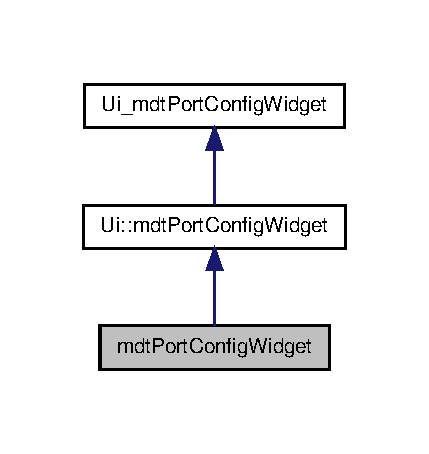
\includegraphics[width=278pt]{classmdt_port_config_widget__inherit__graph}
\end{center}
\end{figure}


Collaboration diagram for mdt\-Port\-Config\-Widget\-:
\nopagebreak
\begin{figure}[H]
\begin{center}
\leavevmode
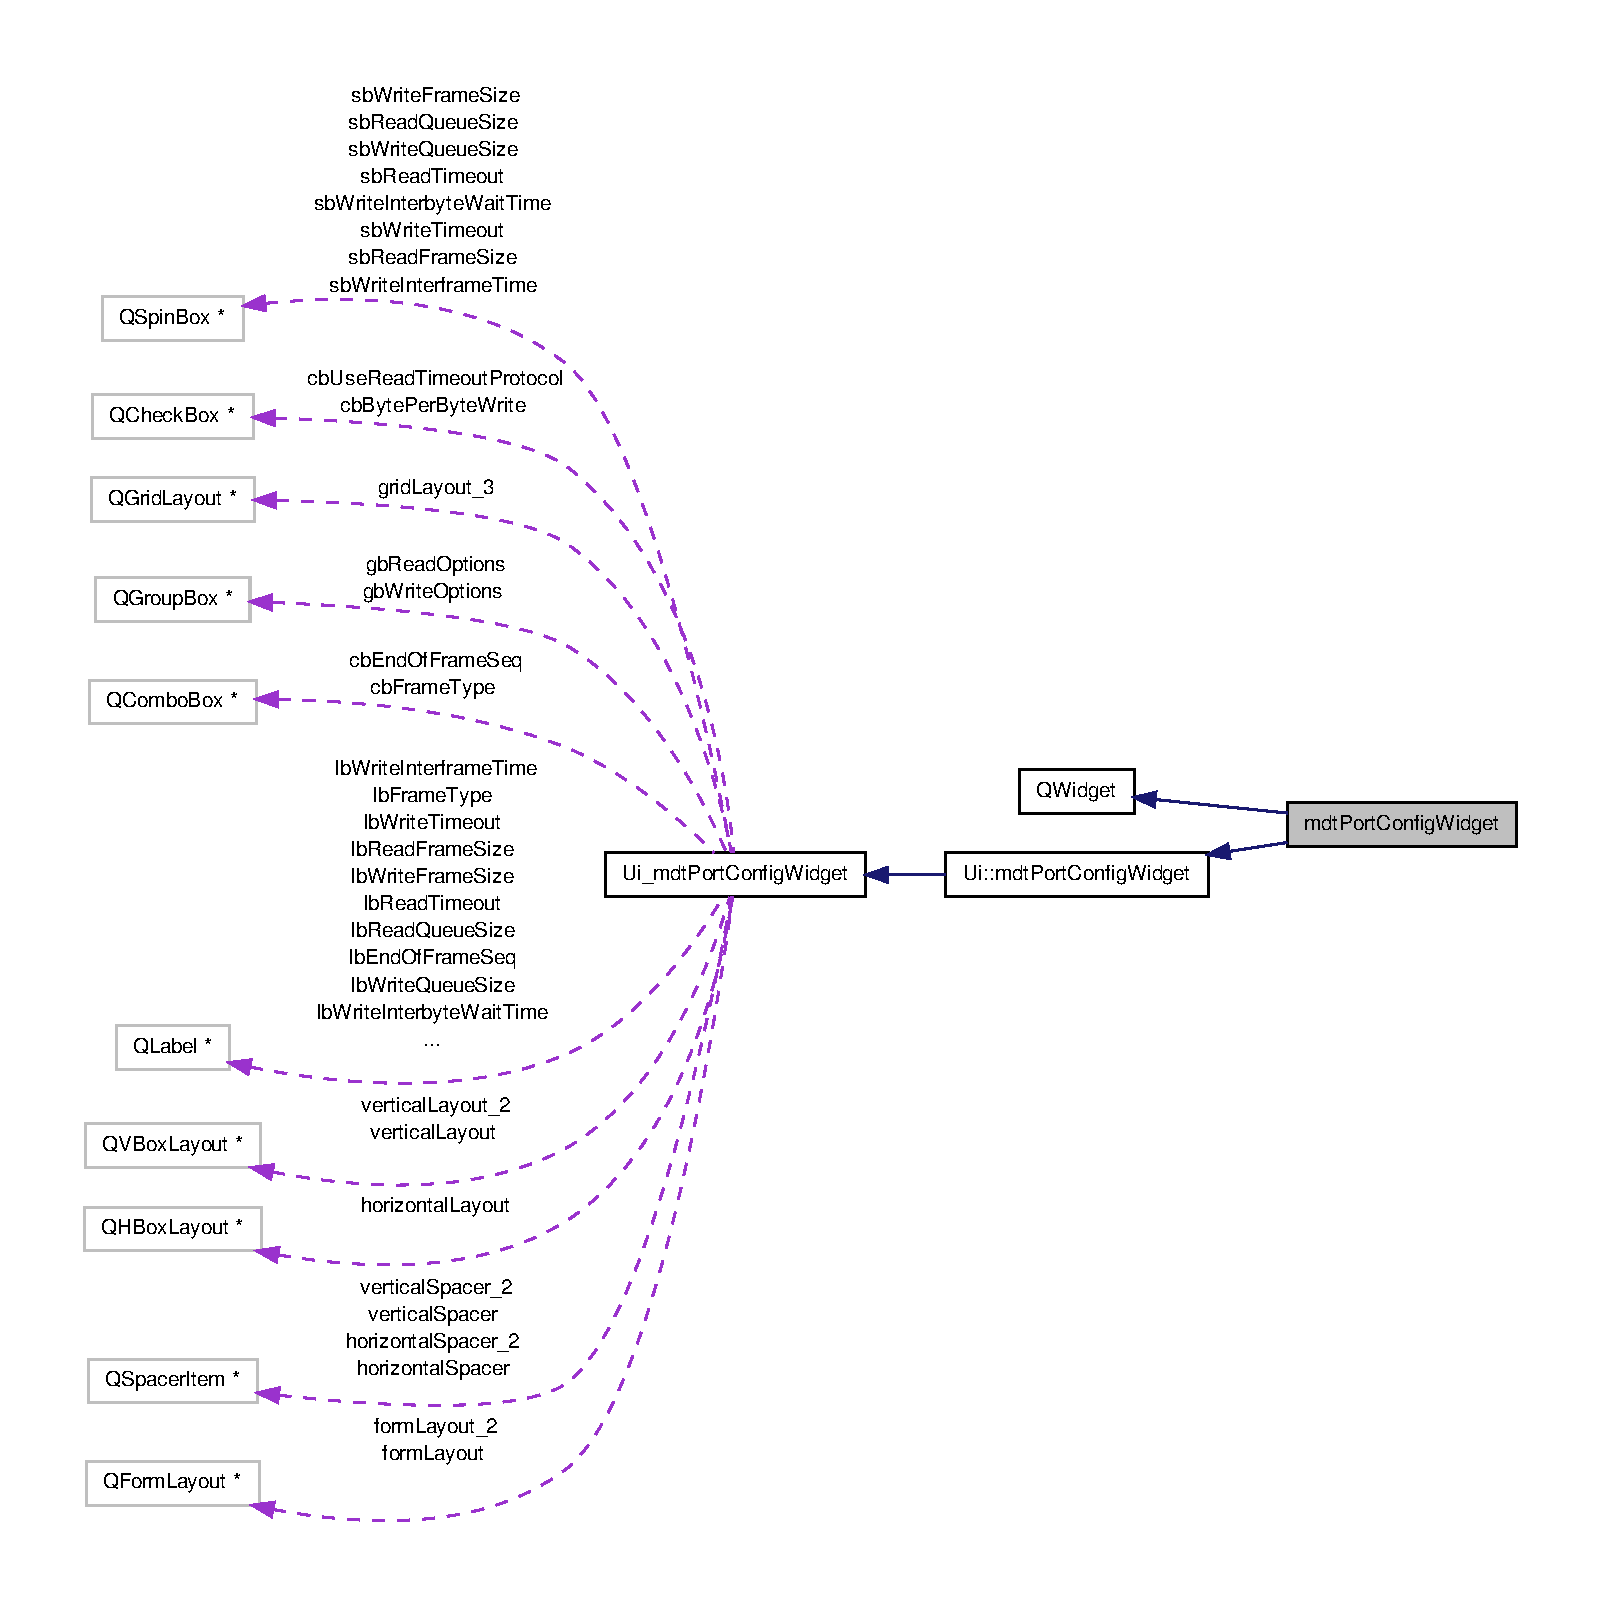
\includegraphics[width=278pt]{classmdt_port_config_widget__coll__graph}
\end{center}
\end{figure}
\subsection*{Public Member Functions}
\begin{DoxyCompactItemize}
\item 
\hyperlink{classmdt_port_config_widget_a5887fadc0001e3438c67de884f8e8f67}{mdt\-Port\-Config\-Widget} (\hyperlink{class_q_widget}{Q\-Widget} $\ast$parent=0)
\item 
void \hyperlink{classmdt_port_config_widget_a44c1690242f5f8680fb4f32a5771534f}{display\-Config} (\hyperlink{classmdt_port_config}{mdt\-Port\-Config} \&config)
\begin{DoxyCompactList}\small\item\em Read the config instance and update G\-U\-I. \end{DoxyCompactList}\item 
void \hyperlink{classmdt_port_config_widget_a23fba4fe5aa0c07b95a9b85218456456}{update\-Config} (\hyperlink{classmdt_port_config}{mdt\-Port\-Config} \&config)
\begin{DoxyCompactList}\small\item\em Get G\-U\-I's selected options and update config. \end{DoxyCompactList}\end{DoxyCompactItemize}


\subsection{Detailed Description}


Definition at line 28 of file mdt\-Port\-Config\-Widget.\-h.



\subsection{Constructor \& Destructor Documentation}
\hypertarget{classmdt_port_config_widget_a5887fadc0001e3438c67de884f8e8f67}{\index{mdt\-Port\-Config\-Widget@{mdt\-Port\-Config\-Widget}!mdt\-Port\-Config\-Widget@{mdt\-Port\-Config\-Widget}}
\index{mdt\-Port\-Config\-Widget@{mdt\-Port\-Config\-Widget}!mdtPortConfigWidget@{mdt\-Port\-Config\-Widget}}
\subsubsection[{mdt\-Port\-Config\-Widget}]{\setlength{\rightskip}{0pt plus 5cm}mdt\-Port\-Config\-Widget\-::mdt\-Port\-Config\-Widget (
\begin{DoxyParamCaption}
\item[{{\bf Q\-Widget} $\ast$}]{parent = {\ttfamily 0}}
\end{DoxyParamCaption}
)}}\label{classmdt_port_config_widget_a5887fadc0001e3438c67de884f8e8f67}


Definition at line 28 of file mdt\-Port\-Config\-Widget.\-cpp.



\subsection{Member Function Documentation}
\hypertarget{classmdt_port_config_widget_a44c1690242f5f8680fb4f32a5771534f}{\index{mdt\-Port\-Config\-Widget@{mdt\-Port\-Config\-Widget}!display\-Config@{display\-Config}}
\index{display\-Config@{display\-Config}!mdtPortConfigWidget@{mdt\-Port\-Config\-Widget}}
\subsubsection[{display\-Config}]{\setlength{\rightskip}{0pt plus 5cm}void mdt\-Port\-Config\-Widget\-::display\-Config (
\begin{DoxyParamCaption}
\item[{{\bf mdt\-Port\-Config} \&}]{config}
\end{DoxyParamCaption}
)}}\label{classmdt_port_config_widget_a44c1690242f5f8680fb4f32a5771534f}


Read the config instance and update G\-U\-I. 



Definition at line 34 of file mdt\-Port\-Config\-Widget.\-cpp.



References mdt\-Port\-Config\-::byte\-Per\-Byte\-Write(), mdt\-Port\-Config\-::end\-Of\-Frame\-Seq(), mdt\-Port\-Config\-::frame\-Type(), mdt\-Frame\-::\-F\-T\-\_\-\-A\-S\-C\-I\-I, mdt\-Frame\-::\-F\-T\-\_\-\-M\-O\-D\-B\-U\-S\-\_\-\-T\-C\-P, mdt\-Frame\-::\-F\-T\-\_\-\-R\-A\-W, mdt\-Frame\-::\-F\-T\-\_\-\-R\-A\-W\-\_\-\-T\-O\-P, mdt\-Frame\-::\-F\-T\-\_\-\-U\-S\-B\-T\-M\-C, mdt\-Port\-Config\-::read\-Frame\-Size(), mdt\-Port\-Config\-::read\-Queue\-Size(), mdt\-Port\-Config\-::read\-Timeout(), mdt\-Port\-Config\-::use\-Read\-Timeout\-Protocol(), mdt\-Port\-Config\-::write\-Frame\-Size(), mdt\-Port\-Config\-::write\-Interbyte\-Time(), mdt\-Port\-Config\-::write\-Interframe\-Time(), mdt\-Port\-Config\-::write\-Queue\-Size(), and mdt\-Port\-Config\-::write\-Timeout().



Referenced by update\-Config().

\hypertarget{classmdt_port_config_widget_a23fba4fe5aa0c07b95a9b85218456456}{\index{mdt\-Port\-Config\-Widget@{mdt\-Port\-Config\-Widget}!update\-Config@{update\-Config}}
\index{update\-Config@{update\-Config}!mdtPortConfigWidget@{mdt\-Port\-Config\-Widget}}
\subsubsection[{update\-Config}]{\setlength{\rightskip}{0pt plus 5cm}void mdt\-Port\-Config\-Widget\-::update\-Config (
\begin{DoxyParamCaption}
\item[{{\bf mdt\-Port\-Config} \&}]{config}
\end{DoxyParamCaption}
)}}\label{classmdt_port_config_widget_a23fba4fe5aa0c07b95a9b85218456456}


Get G\-U\-I's selected options and update config. 

Once done, the config is read again and displayed, so the user can see what was really applied. 

Definition at line 88 of file mdt\-Port\-Config\-Widget.\-cpp.



References display\-Config(), mdt\-Port\-Config\-::frame\-Type(), mdt\-Frame\-::\-F\-T\-\_\-\-A\-S\-C\-I\-I, mdt\-Frame\-::\-F\-T\-\_\-\-M\-O\-D\-B\-U\-S\-\_\-\-T\-C\-P, mdt\-Frame\-::\-F\-T\-\_\-\-R\-A\-W, mdt\-Frame\-::\-F\-T\-\_\-\-R\-A\-W\-\_\-\-T\-O\-P, mdt\-Port\-Config\-::set\-Byte\-Per\-Byte\-Write(), mdt\-Port\-Config\-::set\-End\-Of\-Frame\-Seq(), mdt\-Port\-Config\-::set\-Frame\-Type(), mdt\-Port\-Config\-::set\-Read\-Frame\-Size(), mdt\-Port\-Config\-::set\-Read\-Queue\-Size(), mdt\-Port\-Config\-::set\-Read\-Timeout(), mdt\-Port\-Config\-::set\-Use\-Read\-Timeout\-Protocol(), mdt\-Port\-Config\-::set\-Write\-Frame\-Size(), mdt\-Port\-Config\-::set\-Write\-Interframe\-Time(), mdt\-Port\-Config\-::set\-Write\-Queue\-Size(), and mdt\-Port\-Config\-::set\-Write\-Timeout().



The documentation for this class was generated from the following files\-:\begin{DoxyCompactItemize}
\item 
src/mdtport/\hyperlink{mdt_port_config_widget_8h}{mdt\-Port\-Config\-Widget.\-h}\item 
src/mdtport/\hyperlink{mdt_port_config_widget_8cpp}{mdt\-Port\-Config\-Widget.\-cpp}\end{DoxyCompactItemize}

\hypertarget{classmdt_port_manager}{
\section{mdtPortManager Class Reference}
\label{classmdt_port_manager}\index{mdtPortManager@{mdtPortManager}}
}


Port manager base class.  




{\ttfamily \#include $<$mdtPortManager.h$>$}



Inheritance diagram for mdtPortManager:\nopagebreak
\begin{figure}[H]
\begin{center}
\leavevmode
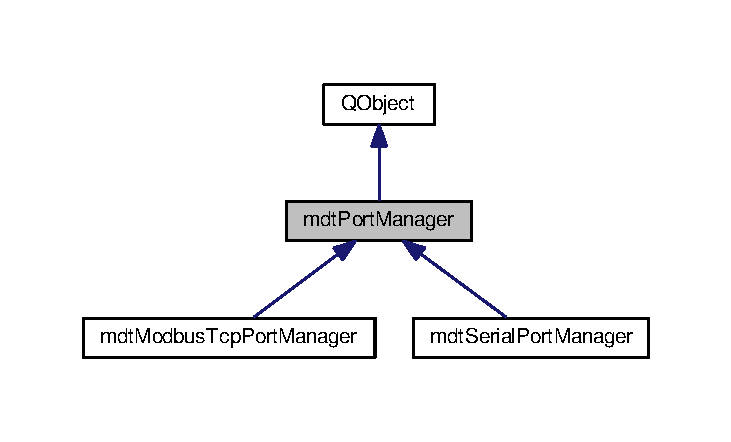
\includegraphics[width=400pt]{classmdt_port_manager__inherit__graph}
\end{center}
\end{figure}


Collaboration diagram for mdtPortManager:\nopagebreak
\begin{figure}[H]
\begin{center}
\leavevmode
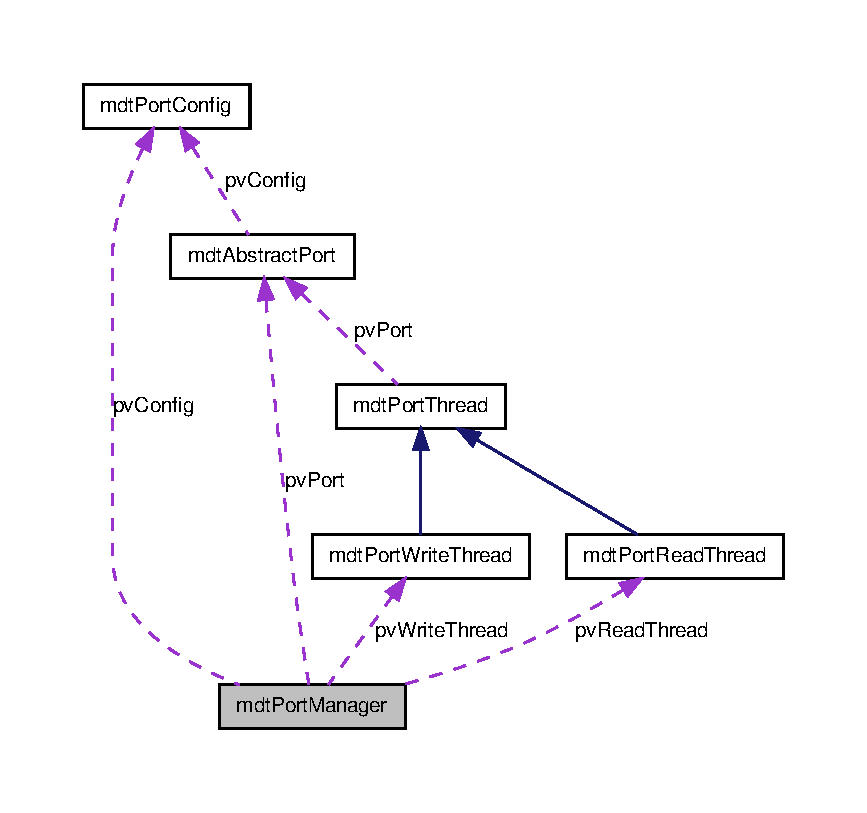
\includegraphics[width=254pt]{classmdt_port_manager__coll__graph}
\end{center}
\end{figure}
\subsection*{Public Slots}
\begin{DoxyCompactItemize}
\item 
virtual void \hyperlink{classmdt_port_manager_a1d185e9bb610aee16ccd9499ae7bff0d}{abort} ()
\begin{DoxyCompactList}\small\item\em Cancel read and write operations. \end{DoxyCompactList}\item 
virtual void \hyperlink{classmdt_port_manager_a4fcc8f0699b655156e661bb3de6056cc}{fromThreadNewFrameReaden} ()
\begin{DoxyCompactList}\small\item\em Try to. \end{DoxyCompactList}\item 
void \hyperlink{classmdt_port_manager_a7e45b8e3475e5182ed12218616664d07}{onThreadsErrorOccured} (int error)
\begin{DoxyCompactList}\small\item\em Manage errors comming from port threads. \end{DoxyCompactList}\end{DoxyCompactItemize}
\subsection*{Signals}
\begin{DoxyCompactItemize}
\item 
void \hyperlink{classmdt_port_manager_abe48be6a56bff4f82842bc31c2746200}{newReadenFrame} ()
\begin{DoxyCompactList}\small\item\em Emitted when new frame was readen. \end{DoxyCompactList}\end{DoxyCompactItemize}
\subsection*{Public Member Functions}
\begin{DoxyCompactItemize}
\item 
\hypertarget{classmdt_port_manager_a5ec36523089b7528d973e29cdbc64d01}{
{\bfseries mdtPortManager} (QObject $\ast$parent=0)}
\label{classmdt_port_manager_a5ec36523089b7528d973e29cdbc64d01}

\item 
virtual \hyperlink{classmdt_port_manager_adf797f8fd7a3ffdc000890a224e4c1b6}{$\sim$mdtPortManager} ()
\begin{DoxyCompactList}\small\item\em Destructor. \end{DoxyCompactList}\item 
virtual QList$<$ \hyperlink{classmdt_port_info}{mdtPortInfo} $\ast$ $>$ \hyperlink{classmdt_port_manager_ad56afb411ab5468005fca04767557ece}{scan} ()
\begin{DoxyCompactList}\small\item\em Scan for available ports. \end{DoxyCompactList}\item 
virtual void \hyperlink{classmdt_port_manager_afcd156b2d0c9d340999935efb6cd8cb6}{setPort} (\hyperlink{classmdt_abstract_port}{mdtAbstractPort} $\ast$port)
\begin{DoxyCompactList}\small\item\em Set port object. \end{DoxyCompactList}\item 
void \hyperlink{classmdt_port_manager_a39cb4af4aedc0b6b7c4d4f53002c3fd1}{detachPort} (bool deletePort, bool deleteThreads)
\begin{DoxyCompactList}\small\item\em Detach port. \end{DoxyCompactList}\item 
void \hyperlink{classmdt_port_manager_ab62591409d019a4a2576b4310c411b8f}{addThread} (\hyperlink{classmdt_port_thread}{mdtPortThread} $\ast$thread)
\begin{DoxyCompactList}\small\item\em Add a thread and assign it to port. \end{DoxyCompactList}\item 
void \hyperlink{classmdt_port_manager_aaa0a474183bcae0fff4fb9ef43023c25}{removeThreads} (bool releaseMemory)
\begin{DoxyCompactList}\small\item\em Detach threads from port and remove threads. \end{DoxyCompactList}\item 
bool \hyperlink{classmdt_port_manager_af1fb103ffafc227337a59c7e82f44fbc}{start} ()
\begin{DoxyCompactList}\small\item\em Start threads. \end{DoxyCompactList}\item 
bool \hyperlink{classmdt_port_manager_af460167e604b8b6e2e933a98b2b6b5a2}{isRunning} ()
\begin{DoxyCompactList}\small\item\em Get the running state. \end{DoxyCompactList}\item 
void \hyperlink{classmdt_port_manager_aacbf87cc3d9c37c87e21696f8a6514bd}{stop} ()
\begin{DoxyCompactList}\small\item\em Stop threads. \end{DoxyCompactList}\item 
void \hyperlink{classmdt_port_manager_a2b2ed690cbba9f544c6ac1b46684e59a}{setPortName} (const QString \&portName)
\begin{DoxyCompactList}\small\item\em Set port name. \end{DoxyCompactList}\item 
void \hyperlink{classmdt_port_manager_a7e2ef93ec2731e66aa2b2d5f7ce9bc1c}{setPortInfo} (\hyperlink{classmdt_port_info}{mdtPortInfo} info)
\begin{DoxyCompactList}\small\item\em Set port info. \end{DoxyCompactList}\item 
\hypertarget{classmdt_port_manager_a88109b455fc5a5f5adf0636f7450143e}{
\hyperlink{classmdt_port_info}{mdtPortInfo} \hyperlink{classmdt_port_manager_a88109b455fc5a5f5adf0636f7450143e}{portInfo} ()}
\label{classmdt_port_manager_a88109b455fc5a5f5adf0636f7450143e}

\begin{DoxyCompactList}\small\item\em Get port info. \end{DoxyCompactList}\item 
virtual \hyperlink{classmdt_port_config}{mdtPortConfig} \& \hyperlink{classmdt_port_manager_a9cf3ea2da38f81682695b37448712ffd}{config} ()
\begin{DoxyCompactList}\small\item\em Get the port's config object. \end{DoxyCompactList}\item 
bool \hyperlink{classmdt_port_manager_aab594613e8985590c835194efbc27b5e}{openPort} ()
\begin{DoxyCompactList}\small\item\em Open the port. \end{DoxyCompactList}\item 
void \hyperlink{classmdt_port_manager_ace8065f1f5083041ee7f65c2892bc77d}{closePort} ()
\begin{DoxyCompactList}\small\item\em Close the port. \end{DoxyCompactList}\item 
virtual int \hyperlink{classmdt_port_manager_a8b60d53d6e553f15dedec916f9c1614b}{writeData} (QByteArray data)
\begin{DoxyCompactList}\small\item\em Write data by copy. \end{DoxyCompactList}\item 
virtual bool \hyperlink{classmdt_port_manager_a44ca338c8c56893612301e09d2ee6e88}{waitReadenFrame} (int timeout=500)
\begin{DoxyCompactList}\small\item\em Wait until a complete frame is available. \end{DoxyCompactList}\item 
QByteArray \hyperlink{classmdt_port_manager_a830ae182d06dd6a52c43a7f45b9240ac}{readenFrame} (int id)
\begin{DoxyCompactList}\small\item\em Get data by frame ID. \end{DoxyCompactList}\item 
QList$<$ QByteArray $>$ \& \hyperlink{classmdt_port_manager_a4843ac996aa5da0df5dc8104ba41b4d8}{readenFrames} ()
\begin{DoxyCompactList}\small\item\em Get all readen data. \end{DoxyCompactList}\item 
void \hyperlink{classmdt_port_manager_acc5c63ad33fdd3cc153fc23e00c6e69c}{wait} (int msecs, int granularity=50)
\begin{DoxyCompactList}\small\item\em Wait some time without break the GUI's event loop. \end{DoxyCompactList}\end{DoxyCompactItemize}
\subsection*{Protected Attributes}
\begin{DoxyCompactItemize}
\item 
\hypertarget{classmdt_port_manager_af856162aab4f1c5202c1dfb330fae538}{
\hyperlink{classmdt_abstract_port}{mdtAbstractPort} $\ast$ {\bfseries pvPort}}
\label{classmdt_port_manager_af856162aab4f1c5202c1dfb330fae538}

\item 
\hypertarget{classmdt_port_manager_a8e0d49b789f8b01d469e84b487799573}{
QList$<$ \hyperlink{classmdt_port_thread}{mdtPortThread} $\ast$ $>$ {\bfseries pvThreads}}
\label{classmdt_port_manager_a8e0d49b789f8b01d469e84b487799573}

\item 
\hypertarget{classmdt_port_manager_a407ff37a8f459bb60288f33f4295ec4f}{
QMap$<$ quint16, QByteArray $>$ {\bfseries pvReadenFrames}}
\label{classmdt_port_manager_a407ff37a8f459bb60288f33f4295ec4f}

\item 
\hypertarget{classmdt_port_manager_afed907a6e33d0439431962aa890976b0}{
QList$<$ QByteArray $>$ {\bfseries pvReadenFramesCopy}}
\label{classmdt_port_manager_afed907a6e33d0439431962aa890976b0}

\end{DoxyCompactItemize}


\subsection{Detailed Description}
Port manager base class. 

Manages a port based on \hyperlink{classmdt_abstract_port}{mdtAbstractPort} an several threads based on \hyperlink{classmdt_port_thread}{mdtPortThread}. The goal is to hide the complexity of the port API.

Example: 
\begin{DoxyCode}
 mdtPortManager m;
 mdtPort *port;
 mdtPortConfig *config;

 // Setup
 config = new mdtPortConfig;
 config->setFrameType(mdtFrame::FT_ASCII);
 config->setEndOfFrameSeq("$");

 // Init port
 port = new mdtPort;
 port->setConfig(config);

 // Init port manager
 m.setPort(port);
 m.addThread(mew mdtPortWriteThread);
 m.addThread(mew mdtPortReadThread);
 m.setPortName("/dev/xyz"));
 if(!m.openPort()){
  // Handle error
 }

 // Start threads
 if(!m.start()){
  // Handle error
 }

 // Send some data
 if(!m.writeData("Test$")){
  // Handle error
 }

 // Wait on answer - Timout: 1500 [ms]
 if(!m.waitReadenFrame(1500)){
  // Timout , handle error
 }

 // Do something with received data
 for(int i=0; i<m.readenFrames().size(); i++){
  qDebug() << m.readenFrames().at(i);
 }

 // Cleanup - detachPort() will delete port and threads objects
 m.detachPort(true, true);
 delete config;
\end{DoxyCode}


A alternative of using \hyperlink{classmdt_port_manager_a44ca338c8c56893612301e09d2ee6e88}{waitReadenFrame()} is to connect the \hyperlink{classmdt_port_manager_abe48be6a56bff4f82842bc31c2746200}{newReadenFrame()} signal to a slot, and get data with \hyperlink{classmdt_port_manager_a4843ac996aa5da0df5dc8104ba41b4d8}{readenFrames()} from this slot.

\begin{DoxySeeAlso}{See also}
\hyperlink{classmdt_serial_port_manager}{mdtSerialPortManager} 

\hyperlink{classmdt_usbtmc_port_manager}{mdtUsbtmcPortManager} (Linux only) 
\end{DoxySeeAlso}


Definition at line 105 of file mdtPortManager.h.



\subsection{Constructor \& Destructor Documentation}
\hypertarget{classmdt_port_manager_adf797f8fd7a3ffdc000890a224e4c1b6}{
\index{mdtPortManager@{mdtPortManager}!$\sim$mdtPortManager@{$\sim$mdtPortManager}}
\index{$\sim$mdtPortManager@{$\sim$mdtPortManager}!mdtPortManager@{mdtPortManager}}
\subsubsection[{$\sim$mdtPortManager}]{\setlength{\rightskip}{0pt plus 5cm}mdtPortManager::$\sim$mdtPortManager (
\begin{DoxyParamCaption}
{}
\end{DoxyParamCaption}
)\hspace{0.3cm}{\ttfamily  \mbox{[}virtual\mbox{]}}}}
\label{classmdt_port_manager_adf797f8fd7a3ffdc000890a224e4c1b6}


Destructor. 

If a port was set, the manager will stop (if running), and port will be closed (if open).

Note that port set by \hyperlink{classmdt_port_manager_afcd156b2d0c9d340999935efb6cd8cb6}{setPort()} and threads are not deleted. 

Definition at line 37 of file mdtPortManager.cpp.



\subsection{Member Function Documentation}
\hypertarget{classmdt_port_manager_a1d185e9bb610aee16ccd9499ae7bff0d}{
\index{mdtPortManager@{mdtPortManager}!abort@{abort}}
\index{abort@{abort}!mdtPortManager@{mdtPortManager}}
\subsubsection[{abort}]{\setlength{\rightskip}{0pt plus 5cm}void mdtPortManager::abort (
\begin{DoxyParamCaption}
{}
\end{DoxyParamCaption}
)\hspace{0.3cm}{\ttfamily  \mbox{[}virtual, slot\mbox{]}}}}
\label{classmdt_port_manager_a1d185e9bb610aee16ccd9499ae7bff0d}


Cancel read and write operations. 

Default implementation calls \hyperlink{classmdt_abstract_port_abde440c49b95833f821e1333c40a7398}{mdtAbstractPort::flush()}. 

pvPort-\/$>$flushIn(); pvPort-\/$>$flushOut(); 



Definition at line 294 of file mdtPortManager.cpp.

\hypertarget{classmdt_port_manager_ab62591409d019a4a2576b4310c411b8f}{
\index{mdtPortManager@{mdtPortManager}!addThread@{addThread}}
\index{addThread@{addThread}!mdtPortManager@{mdtPortManager}}
\subsubsection[{addThread}]{\setlength{\rightskip}{0pt plus 5cm}void mdtPortManager::addThread (
\begin{DoxyParamCaption}
\item[{{\bf mdtPortThread} $\ast$}]{thread}
\end{DoxyParamCaption}
)}}
\label{classmdt_port_manager_ab62591409d019a4a2576b4310c411b8f}


Add a thread and assign it to port. 

\begin{DoxyPrecond}{Precondition}
Port must be set with setPort before using this method 

Manager must no running 

thread must be a valid pointer 
\end{DoxyPrecond}


Definition at line 87 of file mdtPortManager.cpp.

\hypertarget{classmdt_port_manager_ace8065f1f5083041ee7f65c2892bc77d}{
\index{mdtPortManager@{mdtPortManager}!closePort@{closePort}}
\index{closePort@{closePort}!mdtPortManager@{mdtPortManager}}
\subsubsection[{closePort}]{\setlength{\rightskip}{0pt plus 5cm}void mdtPortManager::closePort (
\begin{DoxyParamCaption}
{}
\end{DoxyParamCaption}
)}}
\label{classmdt_port_manager_ace8065f1f5083041ee7f65c2892bc77d}


Close the port. 

This stops the threads (if exists) and close the port.

If port was never set (with \hyperlink{classmdt_port_manager_afcd156b2d0c9d340999935efb6cd8cb6}{setPort()} ), this method does nothing. 

Definition at line 202 of file mdtPortManager.cpp.

\hypertarget{classmdt_port_manager_a9cf3ea2da38f81682695b37448712ffd}{
\index{mdtPortManager@{mdtPortManager}!config@{config}}
\index{config@{config}!mdtPortManager@{mdtPortManager}}
\subsubsection[{config}]{\setlength{\rightskip}{0pt plus 5cm}{\bf mdtPortConfig} \& mdtPortManager::config (
\begin{DoxyParamCaption}
{}
\end{DoxyParamCaption}
)\hspace{0.3cm}{\ttfamily  \mbox{[}virtual\mbox{]}}}}
\label{classmdt_port_manager_a9cf3ea2da38f81682695b37448712ffd}


Get the port's config object. 

Usefull to alter internal port configuration

\begin{DoxyPrecond}{Precondition}
Port must be set with \hyperlink{classmdt_port_manager_afcd156b2d0c9d340999935efb6cd8cb6}{setPort()} before use of this method. 
\end{DoxyPrecond}


Reimplemented in \hyperlink{classmdt_serial_port_manager_a4b8ab7b9d53966a1887d9ce8557b8416}{mdtSerialPortManager}.



Definition at line 184 of file mdtPortManager.cpp.

\hypertarget{classmdt_port_manager_a39cb4af4aedc0b6b7c4d4f53002c3fd1}{
\index{mdtPortManager@{mdtPortManager}!detachPort@{detachPort}}
\index{detachPort@{detachPort}!mdtPortManager@{mdtPortManager}}
\subsubsection[{detachPort}]{\setlength{\rightskip}{0pt plus 5cm}void mdtPortManager::detachPort (
\begin{DoxyParamCaption}
\item[{bool}]{deletePort, }
\item[{bool}]{deleteThreads}
\end{DoxyParamCaption}
)}}
\label{classmdt_port_manager_a39cb4af4aedc0b6b7c4d4f53002c3fd1}


Detach port. 

Will detach port from each thread and from port manager. If port was not set, this method does nothing. If manager is running, it will be stopped. If port is open, it will be closed.


\begin{DoxyParams}{Parameters}
{\em deletePort} & If true, the port object that was set with \hyperlink{classmdt_port_manager_afcd156b2d0c9d340999935efb6cd8cb6}{setPort()} will be deleted. \\
\hline
{\em deleteThreads} & If true, each thread added with \hyperlink{classmdt_port_manager_ab62591409d019a4a2576b4310c411b8f}{addThread()} will be deleted. \\
\hline
\end{DoxyParams}


Definition at line 66 of file mdtPortManager.cpp.

\hypertarget{classmdt_port_manager_a4fcc8f0699b655156e661bb3de6056cc}{
\index{mdtPortManager@{mdtPortManager}!fromThreadNewFrameReaden@{fromThreadNewFrameReaden}}
\index{fromThreadNewFrameReaden@{fromThreadNewFrameReaden}!mdtPortManager@{mdtPortManager}}
\subsubsection[{fromThreadNewFrameReaden}]{\setlength{\rightskip}{0pt plus 5cm}void mdtPortManager::fromThreadNewFrameReaden (
\begin{DoxyParamCaption}
{}
\end{DoxyParamCaption}
)\hspace{0.3cm}{\ttfamily  \mbox{[}virtual, slot\mbox{]}}}}
\label{classmdt_port_manager_a4fcc8f0699b655156e661bb3de6056cc}


Try to. 

Called by the read thread whenn a complete frame was readen

\begin{DoxySeeAlso}{See also}
\hyperlink{classmdt_port_thread}{mdtPortThread} 
\end{DoxySeeAlso}


\begin{Desc}
\item[\hyperlink{todo__todo000026}{Todo}]Error on incomplete frame \end{Desc}




Reimplemented in \hyperlink{classmdt_modbus_tcp_port_manager_ad941ea607f00db54aa6deb2866a539e9}{mdtModbusTcpPortManager}, and \hyperlink{classmdt_usbtmc_port_manager_aca42b343ae1f6a324e6e45968f03bbea}{mdtUsbtmcPortManager}.



Definition at line 303 of file mdtPortManager.cpp.

\hypertarget{classmdt_port_manager_af460167e604b8b6e2e933a98b2b6b5a2}{
\index{mdtPortManager@{mdtPortManager}!isRunning@{isRunning}}
\index{isRunning@{isRunning}!mdtPortManager@{mdtPortManager}}
\subsubsection[{isRunning}]{\setlength{\rightskip}{0pt plus 5cm}bool mdtPortManager::isRunning (
\begin{DoxyParamCaption}
{}
\end{DoxyParamCaption}
)}}
\label{classmdt_port_manager_af460167e604b8b6e2e933a98b2b6b5a2}


Get the running state. 

If one of the threads is running, true is returned.

If port was not set, it returns false. 

Definition at line 138 of file mdtPortManager.cpp.

\hypertarget{classmdt_port_manager_abe48be6a56bff4f82842bc31c2746200}{
\index{mdtPortManager@{mdtPortManager}!newReadenFrame@{newReadenFrame}}
\index{newReadenFrame@{newReadenFrame}!mdtPortManager@{mdtPortManager}}
\subsubsection[{newReadenFrame}]{\setlength{\rightskip}{0pt plus 5cm}void mdtPortManager::newReadenFrame (
\begin{DoxyParamCaption}
{}
\end{DoxyParamCaption}
)\hspace{0.3cm}{\ttfamily  \mbox{[}signal\mbox{]}}}}
\label{classmdt_port_manager_abe48be6a56bff4f82842bc31c2746200}


Emitted when new frame was readen. 

\begin{DoxySeeAlso}{See also}
\hyperlink{classmdt_port_manager_a44ca338c8c56893612301e09d2ee6e88}{waitReadenFrame()} 
\end{DoxySeeAlso}
\hypertarget{classmdt_port_manager_a7e45b8e3475e5182ed12218616664d07}{
\index{mdtPortManager@{mdtPortManager}!onThreadsErrorOccured@{onThreadsErrorOccured}}
\index{onThreadsErrorOccured@{onThreadsErrorOccured}!mdtPortManager@{mdtPortManager}}
\subsubsection[{onThreadsErrorOccured}]{\setlength{\rightskip}{0pt plus 5cm}void mdtPortManager::onThreadsErrorOccured (
\begin{DoxyParamCaption}
\item[{int}]{error}
\end{DoxyParamCaption}
)\hspace{0.3cm}{\ttfamily  \mbox{[}slot\mbox{]}}}}
\label{classmdt_port_manager_a7e45b8e3475e5182ed12218616664d07}


Manage errors comming from port threads. 

\begin{Desc}
\item[\hyperlink{todo__todo000027}{Todo}]Error handling (in general ...) \end{Desc}


if(error == MDT\_\-PORT\_\-IO\_\-ERROR)\{ qDebug() $<$$<$ \char`\"{}I/O error !\char`\"{}; \hyperlink{classmdt_port_manager_ace8065f1f5083041ee7f65c2892bc77d}{closePort()}; if(!openPort())\{ return; \} \hyperlink{classmdt_port_manager_af1fb103ffafc227337a59c7e82f44fbc}{start()}; \} if(error == MDT\_\-PORT\_\-QUEUE\_\-EMPTY\_\-ERROR)\{ qDebug() $<$$<$ \char`\"{}Queue empty !\char`\"{}; \}



Definition at line 330 of file mdtPortManager.cpp.

\hypertarget{classmdt_port_manager_aab594613e8985590c835194efbc27b5e}{
\index{mdtPortManager@{mdtPortManager}!openPort@{openPort}}
\index{openPort@{openPort}!mdtPortManager@{mdtPortManager}}
\subsubsection[{openPort}]{\setlength{\rightskip}{0pt plus 5cm}bool mdtPortManager::openPort (
\begin{DoxyParamCaption}
{}
\end{DoxyParamCaption}
)}}
\label{classmdt_port_manager_aab594613e8985590c835194efbc27b5e}


Open the port. 

Will try to open port defined with \hyperlink{classmdt_port_manager_a2b2ed690cbba9f544c6ac1b46684e59a}{setPortName()}.

\begin{DoxyReturn}{Returns}
True on success, false else. 
\end{DoxyReturn}
\begin{DoxyPrecond}{Precondition}
Port must be set with \hyperlink{classmdt_port_manager_afcd156b2d0c9d340999935efb6cd8cb6}{setPort()} before use of this method. 
\end{DoxyPrecond}


Definition at line 191 of file mdtPortManager.cpp.

\hypertarget{classmdt_port_manager_a830ae182d06dd6a52c43a7f45b9240ac}{
\index{mdtPortManager@{mdtPortManager}!readenFrame@{readenFrame}}
\index{readenFrame@{readenFrame}!mdtPortManager@{mdtPortManager}}
\subsubsection[{readenFrame}]{\setlength{\rightskip}{0pt plus 5cm}QByteArray mdtPortManager::readenFrame (
\begin{DoxyParamCaption}
\item[{int}]{id}
\end{DoxyParamCaption}
)}}
\label{classmdt_port_manager_a830ae182d06dd6a52c43a7f45b9240ac}


Get data by frame ID. 

The frame ID is a protocol specific identification. F.ex. in MODBUS/TCP, the transaction ID is used, or bTag for USBTMC.

If found, the frame is removed from received queue.

If ID was not found, a empty QByteArray is returned. 

Definition at line 256 of file mdtPortManager.cpp.

\hypertarget{classmdt_port_manager_a4843ac996aa5da0df5dc8104ba41b4d8}{
\index{mdtPortManager@{mdtPortManager}!readenFrames@{readenFrames}}
\index{readenFrames@{readenFrames}!mdtPortManager@{mdtPortManager}}
\subsubsection[{readenFrames}]{\setlength{\rightskip}{0pt plus 5cm}QList$<$ QByteArray $>$ \& mdtPortManager::readenFrames (
\begin{DoxyParamCaption}
{}
\end{DoxyParamCaption}
)}}
\label{classmdt_port_manager_a4843ac996aa5da0df5dc8104ba41b4d8}


Get all readen data. 

Get a copy of all currently available data. Data frames are sorted by asending order, i.e. if frame ID is used, the sort order is this ID assending, else it is from oldest to newest received frame (like a FIFO).

After a call of this method, the internal received frames queue is cleared.

Note: the list of returned data (witch is a copy of reception queue) must be cleared explicitly with QList::clear() after data are used. (or remove each item with, for.ex. QList::takeFirst() ) 

Definition at line 267 of file mdtPortManager.cpp.

\hypertarget{classmdt_port_manager_aaa0a474183bcae0fff4fb9ef43023c25}{
\index{mdtPortManager@{mdtPortManager}!removeThreads@{removeThreads}}
\index{removeThreads@{removeThreads}!mdtPortManager@{mdtPortManager}}
\subsubsection[{removeThreads}]{\setlength{\rightskip}{0pt plus 5cm}void mdtPortManager::removeThreads (
\begin{DoxyParamCaption}
\item[{bool}]{releaseMemory}
\end{DoxyParamCaption}
)}}
\label{classmdt_port_manager_aaa0a474183bcae0fff4fb9ef43023c25}


Detach threads from port and remove threads. 


\begin{DoxyParams}{Parameters}
{\em releaseMemory} & If true, all threads are deleted \\
\hline
\end{DoxyParams}
\begin{DoxyPrecond}{Precondition}
Port manager must not running. 
\end{DoxyPrecond}


Definition at line 103 of file mdtPortManager.cpp.

\hypertarget{classmdt_port_manager_ad56afb411ab5468005fca04767557ece}{
\index{mdtPortManager@{mdtPortManager}!scan@{scan}}
\index{scan@{scan}!mdtPortManager@{mdtPortManager}}
\subsubsection[{scan}]{\setlength{\rightskip}{0pt plus 5cm}QList$<$ {\bf mdtPortInfo} $\ast$ $>$ mdtPortManager::scan (
\begin{DoxyParamCaption}
{}
\end{DoxyParamCaption}
)\hspace{0.3cm}{\ttfamily  \mbox{[}virtual\mbox{]}}}}
\label{classmdt_port_manager_ad56afb411ab5468005fca04767557ece}


Scan for available ports. 

This method is implemented is port's specific subclass. Default implementation returns a empty list.

Note that returned list must be freed by user after usage. (for.ex. with qDeletAll() and QList::clear() ).

\begin{DoxyPrecond}{Precondition}
Manager must no running 
\end{DoxyPrecond}


Reimplemented in \hyperlink{classmdt_usbtmc_port_manager_a992d1227810186d3c7dc166452e2e3b6}{mdtUsbtmcPortManager}, and \hyperlink{classmdt_serial_port_manager_a791572f869d1d605d0c4658ca4187260}{mdtSerialPortManager}.



Definition at line 51 of file mdtPortManager.cpp.

\hypertarget{classmdt_port_manager_afcd156b2d0c9d340999935efb6cd8cb6}{
\index{mdtPortManager@{mdtPortManager}!setPort@{setPort}}
\index{setPort@{setPort}!mdtPortManager@{mdtPortManager}}
\subsubsection[{setPort}]{\setlength{\rightskip}{0pt plus 5cm}void mdtPortManager::setPort (
\begin{DoxyParamCaption}
\item[{{\bf mdtAbstractPort} $\ast$}]{port}
\end{DoxyParamCaption}
)\hspace{0.3cm}{\ttfamily  \mbox{[}virtual\mbox{]}}}}
\label{classmdt_port_manager_afcd156b2d0c9d340999935efb6cd8cb6}


Set port object. 

\begin{DoxyPrecond}{Precondition}
port must be a valid pointer to the expected class instance (for ex: \hyperlink{classmdt_serial_port}{mdtSerialPort}). 

Manager must no running 
\end{DoxyPrecond}


Definition at line 58 of file mdtPortManager.cpp.

\hypertarget{classmdt_port_manager_a7e2ef93ec2731e66aa2b2d5f7ce9bc1c}{
\index{mdtPortManager@{mdtPortManager}!setPortInfo@{setPortInfo}}
\index{setPortInfo@{setPortInfo}!mdtPortManager@{mdtPortManager}}
\subsubsection[{setPortInfo}]{\setlength{\rightskip}{0pt plus 5cm}void mdtPortManager::setPortInfo (
\begin{DoxyParamCaption}
\item[{{\bf mdtPortInfo}}]{info}
\end{DoxyParamCaption}
)}}
\label{classmdt_port_manager_a7e2ef93ec2731e66aa2b2d5f7ce9bc1c}


Set port info. 

Store given port info, and call \hyperlink{classmdt_port_manager_a2b2ed690cbba9f544c6ac1b46684e59a}{setPortName()} with port info's stored port name (see \hyperlink{classmdt_port_info_ad456aac33dccc9b0583ed8aa4796cdf0}{mdtPortInfo::portName()} ).

Setting a port info can be usefull if other informations are needed later in application (f.ex. \hyperlink{classmdt_port_info_a38bcac67372782228a91d8e7dbf49211}{mdtPortInfo::displayText()} ). You can get port informations later with \hyperlink{classmdt_port_manager_a88109b455fc5a5f5adf0636f7450143e}{portInfo()}. 

Definition at line 173 of file mdtPortManager.cpp.

\hypertarget{classmdt_port_manager_a2b2ed690cbba9f544c6ac1b46684e59a}{
\index{mdtPortManager@{mdtPortManager}!setPortName@{setPortName}}
\index{setPortName@{setPortName}!mdtPortManager@{mdtPortManager}}
\subsubsection[{setPortName}]{\setlength{\rightskip}{0pt plus 5cm}void mdtPortManager::setPortName (
\begin{DoxyParamCaption}
\item[{const QString \&}]{portName}
\end{DoxyParamCaption}
)}}
\label{classmdt_port_manager_a2b2ed690cbba9f544c6ac1b46684e59a}


Set port name. 

Set the port name to internally port object. Does nothing else. To open the port, use \hyperlink{classmdt_port_manager_aab594613e8985590c835194efbc27b5e}{openPort()}.

\begin{DoxyPrecond}{Precondition}
Port must be set before with \hyperlink{classmdt_port_manager_afcd156b2d0c9d340999935efb6cd8cb6}{setPort()} 
\end{DoxyPrecond}
\begin{DoxySeeAlso}{See also}
\hyperlink{classmdt_abstract_port}{mdtAbstractPort} 
\end{DoxySeeAlso}


Definition at line 166 of file mdtPortManager.cpp.

\hypertarget{classmdt_port_manager_af1fb103ffafc227337a59c7e82f44fbc}{
\index{mdtPortManager@{mdtPortManager}!start@{start}}
\index{start@{start}!mdtPortManager@{mdtPortManager}}
\subsubsection[{start}]{\setlength{\rightskip}{0pt plus 5cm}bool mdtPortManager::start (
\begin{DoxyParamCaption}
{}
\end{DoxyParamCaption}
)}}
\label{classmdt_port_manager_af1fb103ffafc227337a59c7e82f44fbc}


Start threads. 

\begin{DoxyPrecond}{Precondition}
Port must be set with \hyperlink{classmdt_port_manager_afcd156b2d0c9d340999935efb6cd8cb6}{setPort()} before use of this method. 
\end{DoxyPrecond}


Definition at line 123 of file mdtPortManager.cpp.

\hypertarget{classmdt_port_manager_aacbf87cc3d9c37c87e21696f8a6514bd}{
\index{mdtPortManager@{mdtPortManager}!stop@{stop}}
\index{stop@{stop}!mdtPortManager@{mdtPortManager}}
\subsubsection[{stop}]{\setlength{\rightskip}{0pt plus 5cm}void mdtPortManager::stop (
\begin{DoxyParamCaption}
{}
\end{DoxyParamCaption}
)}}
\label{classmdt_port_manager_aacbf87cc3d9c37c87e21696f8a6514bd}


Stop threads. 

\begin{DoxyPrecond}{Precondition}
Port must be set with \hyperlink{classmdt_port_manager_afcd156b2d0c9d340999935efb6cd8cb6}{setPort()} before use of this method. 
\end{DoxyPrecond}


Definition at line 155 of file mdtPortManager.cpp.

\hypertarget{classmdt_port_manager_acc5c63ad33fdd3cc153fc23e00c6e69c}{
\index{mdtPortManager@{mdtPortManager}!wait@{wait}}
\index{wait@{wait}!mdtPortManager@{mdtPortManager}}
\subsubsection[{wait}]{\setlength{\rightskip}{0pt plus 5cm}void mdtPortManager::wait (
\begin{DoxyParamCaption}
\item[{int}]{msecs, }
\item[{int}]{granularity = {\ttfamily 50}}
\end{DoxyParamCaption}
)}}
\label{classmdt_port_manager_acc5c63ad33fdd3cc153fc23e00c6e69c}


Wait some time without break the GUI's event loop. 

This is a helper method that provide a blocking wait. Internally, a couple of sleep and event processing is done, avoiding freesing the GUI.

This wait method is not precise.


\begin{DoxyParams}{Parameters}
{\em msecs} & Time to wait \mbox{[}ms\mbox{]} \\
\hline
{\em granularity} & Sleep time between each call of event processing \mbox{[}ms\mbox{]}\par
 A little value needs more CPU and big value can freese the GUI. Should be between 50 and 100, and must be $>$ 0. Note that msecs must be a multiple of granularity. \\
\hline
\end{DoxyParams}
\begin{DoxyPrecond}{Precondition}
granularity must be $>$ 0. 
\end{DoxyPrecond}


Definition at line 281 of file mdtPortManager.cpp.

\hypertarget{classmdt_port_manager_a44ca338c8c56893612301e09d2ee6e88}{
\index{mdtPortManager@{mdtPortManager}!waitReadenFrame@{waitReadenFrame}}
\index{waitReadenFrame@{waitReadenFrame}!mdtPortManager@{mdtPortManager}}
\subsubsection[{waitReadenFrame}]{\setlength{\rightskip}{0pt plus 5cm}bool mdtPortManager::waitReadenFrame (
\begin{DoxyParamCaption}
\item[{int}]{timeout = {\ttfamily 500}}
\end{DoxyParamCaption}
)\hspace{0.3cm}{\ttfamily  \mbox{[}virtual\mbox{]}}}}
\label{classmdt_port_manager_a44ca338c8c56893612301e09d2ee6e88}


Wait until a complete frame is available. 

This method will return when a complete frame was readen. This is usefull for query/answer protocols.

Internally, a couple of sleep and process event are called, so Qt's event loop will not be broken.


\begin{DoxyParams}{Parameters}
{\em timeout} & Maximum wait time \mbox{[}ms\mbox{]}. Must be a multiple of 50 \mbox{[}ms\mbox{]} \\
\hline
\end{DoxyParams}
\begin{DoxyReturn}{Returns}
True if Ok, false on timeout 
\end{DoxyReturn}
\begin{DoxySeeAlso}{See also}
\hyperlink{classmdt_port_manager_abe48be6a56bff4f82842bc31c2746200}{newReadenFrame()}
\end{DoxySeeAlso}
Subclass notes:\par
 This method can be reimplemented in subclass if needed. 

Definition at line 240 of file mdtPortManager.cpp.

\hypertarget{classmdt_port_manager_a8b60d53d6e553f15dedec916f9c1614b}{
\index{mdtPortManager@{mdtPortManager}!writeData@{writeData}}
\index{writeData@{writeData}!mdtPortManager@{mdtPortManager}}
\subsubsection[{writeData}]{\setlength{\rightskip}{0pt plus 5cm}int mdtPortManager::writeData (
\begin{DoxyParamCaption}
\item[{QByteArray}]{data}
\end{DoxyParamCaption}
)\hspace{0.3cm}{\ttfamily  \mbox{[}virtual\mbox{]}}}}
\label{classmdt_port_manager_a8b60d53d6e553f15dedec916f9c1614b}


Write data by copy. 

Data will be passed to the mdtPort's write queue by copy. This method returns immediatly after enqueue, and don't wait until data was written.


\begin{DoxyParams}{Parameters}
{\em data} & Data to write \\
\hline
\end{DoxyParams}
\begin{DoxyReturn}{Returns}
0 on success or value $<$ 0 if write queue is full. Some subclass can return a frame ID, see subclass documentation for details. 
\end{DoxyReturn}
\begin{DoxyPrecond}{Precondition}
Port must be set with \hyperlink{classmdt_port_manager_afcd156b2d0c9d340999935efb6cd8cb6}{setPort()} before use of this method.
\end{DoxyPrecond}
Subclass notes:\par
 This method can be reimplemented in subclass if needed. Typically usefull if some encoding is needed before the frame is submitted to port. A frame must be taken from port's write frames pool with \hyperlink{classmdt_abstract_port_abf093b67fddebffa4f3c52277b9a8cf7}{mdtAbstractPort::writeFramesPool()} dequeue() method (see Qt's QQueue documentation for more details on dequeue() ), then added to port's write queue with \hyperlink{classmdt_abstract_port_a9a69eb2fc07d551ab37c011487fa319d}{mdtAbstractPort::addFrameToWrite()} . If protocol supports frame identification (like MODBUS's transaction ID or USBTMC's bTag), it should be returned here and incremented. 

Reimplemented in \hyperlink{classmdt_modbus_tcp_port_manager_a0c56b7d38cfb52d95e81de4ca6ac414f}{mdtModbusTcpPortManager}, and \hyperlink{classmdt_usbtmc_port_manager_ab7229e9d519e80a6509bec90dc9239b3}{mdtUsbtmcPortManager}.



Definition at line 213 of file mdtPortManager.cpp.



The documentation for this class was generated from the following files:\begin{DoxyCompactItemize}
\item 
src/mdtport/mdtPortManager.h\item 
src/mdtport/mdtPortManager.cpp\end{DoxyCompactItemize}

\hypertarget{classmdt_port_posix}{
\section{mdtPortPosix Class Reference}
\label{classmdt_port_posix}\index{mdtPortPosix@{mdtPortPosix}}
}


Inheritance diagram for mdtPortPosix:
\nopagebreak
\begin{figure}[H]
\begin{center}
\leavevmode
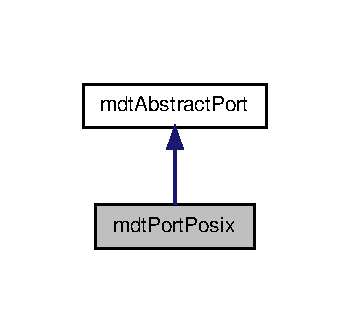
\includegraphics[width=168pt]{classmdt_port_posix__inherit__graph}
\end{center}
\end{figure}


Collaboration diagram for mdtPortPosix:
\nopagebreak
\begin{figure}[H]
\begin{center}
\leavevmode
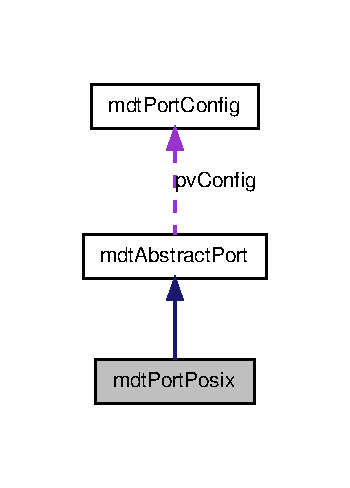
\includegraphics[width=168pt]{classmdt_port_posix__coll__graph}
\end{center}
\end{figure}
\subsection*{Public Member Functions}
\begin{DoxyCompactItemize}
\item 
\hypertarget{classmdt_port_posix_ac122e8dde0e224afb3557d29a62de114}{
{\bfseries mdtPortPosix} (QObject $\ast$parent=0)}
\label{classmdt_port_posix_ac122e8dde0e224afb3557d29a62de114}

\item 
bool \hyperlink{classmdt_port_posix_a32a532f5148226da19ee4acc6ec63201}{setAttributes} (const QString \&portName)
\begin{DoxyCompactList}\small\item\em Set the port attributes. \end{DoxyCompactList}\item 
bool \hyperlink{classmdt_port_posix_aba7e87cb2423bfd61a248cc5d23a8517}{open} (\hyperlink{classmdt_port_config}{mdtPortConfig} \&cfg)
\begin{DoxyCompactList}\small\item\em Open the port. \end{DoxyCompactList}\item 
void \hyperlink{classmdt_port_posix_a778c8d4f6fadd1da725f4287af38f7f0}{close} ()
\begin{DoxyCompactList}\small\item\em Close the port. \end{DoxyCompactList}\item 
void \hyperlink{classmdt_port_posix_a7ab7e4a7dccbd58702f2c37335b900c8}{setReadTimeout} (int timeout)
\begin{DoxyCompactList}\small\item\em Set the read data timeout. \end{DoxyCompactList}\item 
void \hyperlink{classmdt_port_posix_a577a51bf0373f478b32bb1c1e5c4726c}{setWriteTimeout} (int timeout)
\begin{DoxyCompactList}\small\item\em Set the write data timeout. \end{DoxyCompactList}\item 
bool \hyperlink{classmdt_port_posix_a5547db404f974f1a04ba2e303b0aaed0}{waitForReadyRead} ()
\begin{DoxyCompactList}\small\item\em Wait until data is available at device. \end{DoxyCompactList}\item 
qint64 \hyperlink{classmdt_port_posix_a1940fad77c70b3c2b7e9ae2b117f4e41}{read} (char $\ast$data, qint64 maxSize)
\begin{DoxyCompactList}\small\item\em Read data from port. \end{DoxyCompactList}\item 
bool \hyperlink{classmdt_port_posix_a6dc329dcaf343a471cf09379f563fa06}{waitEventWriteReady} ()
\begin{DoxyCompactList}\small\item\em Wait until data can be written to device. \end{DoxyCompactList}\item 
qint64 \hyperlink{classmdt_port_posix_a78e35734ae3088be2f2b097225bd648f}{write} (const char $\ast$data, qint64 maxSize)
\begin{DoxyCompactList}\small\item\em Write data to port. \end{DoxyCompactList}\end{DoxyCompactItemize}
\subsection*{Protected Attributes}
\begin{DoxyCompactItemize}
\item 
\hypertarget{classmdt_port_posix_a84faa907c02ae2e6714c2bf2c23e2cf1}{
int {\bfseries pvFd}}
\label{classmdt_port_posix_a84faa907c02ae2e6714c2bf2c23e2cf1}

\end{DoxyCompactItemize}


\subsection{Member Function Documentation}
\hypertarget{classmdt_port_posix_a778c8d4f6fadd1da725f4287af38f7f0}{
\index{mdtPortPosix@{mdtPortPosix}!close@{close}}
\index{close@{close}!mdtPortPosix@{mdtPortPosix}}
\subsubsection[{close}]{\setlength{\rightskip}{0pt plus 5cm}void mdtPortPosix::close (
\begin{DoxyParamCaption}
{}
\end{DoxyParamCaption}
)\hspace{0.3cm}{\ttfamily  \mbox{[}virtual\mbox{]}}}}
\label{classmdt_port_posix_a778c8d4f6fadd1da725f4287af38f7f0}


Close the port. 

This method must be re-\/implemented in subclass.\par
 To handle the port correctly, the subclass method must:
\begin{DoxyItemize}
\item Lock the mutex with \hyperlink{classmdt_abstract_port_a6bf2ecdcf894da3929a22eb8793a9fe3}{lockMutex()}
\item Do the specific work
\item Call this close method (with \hyperlink{classmdt_abstract_port_a1ace1a2bd1a04f16952980e247b04800}{mdtAbstractPort::close()} ). At this last step, the queues will be deleted, and mutex unocked. 
\end{DoxyItemize}

Reimplemented from \hyperlink{classmdt_abstract_port_a1ace1a2bd1a04f16952980e247b04800}{mdtAbstractPort}.

\hypertarget{classmdt_port_posix_aba7e87cb2423bfd61a248cc5d23a8517}{
\index{mdtPortPosix@{mdtPortPosix}!open@{open}}
\index{open@{open}!mdtPortPosix@{mdtPortPosix}}
\subsubsection[{open}]{\setlength{\rightskip}{0pt plus 5cm}bool mdtPortPosix::open (
\begin{DoxyParamCaption}
\item[{{\bf mdtPortConfig} \&}]{cfg}
\end{DoxyParamCaption}
)\hspace{0.3cm}{\ttfamily  \mbox{[}virtual\mbox{]}}}}
\label{classmdt_port_posix_aba7e87cb2423bfd61a248cc5d23a8517}


Open the port. 

This method must be re-\/implemented in subclass.\par
 To handle the port correctly, the subclass method must:
\begin{DoxyItemize}
\item Close previous opened ressource
\item Lock the mutex with \hyperlink{classmdt_abstract_port_a6bf2ecdcf894da3929a22eb8793a9fe3}{lockMutex()}
\item Do the specific work
\item Set the read/write timeouts. See the \hyperlink{classmdt_port_config}{mdtPortConfig} to know how to get these timeouts.
\item Call this open method (with \hyperlink{classmdt_abstract_port_a4a8195c2bf580eb69ad5d90de86798e6}{mdtAbstractPort::open()} ). At this last step, the queues will be initialized, and mutex unocked. \begin{DoxyReturn}{Returns}
True on successfull configuration and open port 
\end{DoxyReturn}
\begin{DoxySeeAlso}{See also}
\hyperlink{classmdt_port_config}{mdtPortConfig} 
\end{DoxySeeAlso}

\end{DoxyItemize}

Reimplemented from \hyperlink{classmdt_abstract_port_a4a8195c2bf580eb69ad5d90de86798e6}{mdtAbstractPort}.

\hypertarget{classmdt_port_posix_a1940fad77c70b3c2b7e9ae2b117f4e41}{
\index{mdtPortPosix@{mdtPortPosix}!read@{read}}
\index{read@{read}!mdtPortPosix@{mdtPortPosix}}
\subsubsection[{read}]{\setlength{\rightskip}{0pt plus 5cm}qint64 mdtPortPosix::read (
\begin{DoxyParamCaption}
\item[{char $\ast$}]{data, }
\item[{qint64}]{maxSize}
\end{DoxyParamCaption}
)\hspace{0.3cm}{\ttfamily  \mbox{[}virtual\mbox{]}}}}
\label{classmdt_port_posix_a1940fad77c70b3c2b7e9ae2b117f4e41}


Read data from port. 

This method must be implemented in subclass \begin{DoxyReturn}{Returns}
Number of bytes readen, or $<$0 on error 
\end{DoxyReturn}


Implements \hyperlink{classmdt_abstract_port_a9d9c45220d5328c9856a2445557fe970}{mdtAbstractPort}.

\hypertarget{classmdt_port_posix_a32a532f5148226da19ee4acc6ec63201}{
\index{mdtPortPosix@{mdtPortPosix}!setAttributes@{setAttributes}}
\index{setAttributes@{setAttributes}!mdtPortPosix@{mdtPortPosix}}
\subsubsection[{setAttributes}]{\setlength{\rightskip}{0pt plus 5cm}bool mdtPortPosix::setAttributes (
\begin{DoxyParamCaption}
\item[{const QString \&}]{portName}
\end{DoxyParamCaption}
)\hspace{0.3cm}{\ttfamily  \mbox{[}virtual\mbox{]}}}}
\label{classmdt_port_posix_a32a532f5148226da19ee4acc6ec63201}


Set the port attributes. 

Open the given port name and get his attributes. This method must be re-\/implemented in subclass. 
\begin{DoxyParams}{Parameters}
{\em portName} & Name of the port to open (f.ex: /dev/ttyS0 , COM1, ...) \\
\hline
\end{DoxyParams}


Implements \hyperlink{classmdt_abstract_port_af143cb0985d15c1c30da30cc7de206a7}{mdtAbstractPort}.

\hypertarget{classmdt_port_posix_a7ab7e4a7dccbd58702f2c37335b900c8}{
\index{mdtPortPosix@{mdtPortPosix}!setReadTimeout@{setReadTimeout}}
\index{setReadTimeout@{setReadTimeout}!mdtPortPosix@{mdtPortPosix}}
\subsubsection[{setReadTimeout}]{\setlength{\rightskip}{0pt plus 5cm}void mdtPortPosix::setReadTimeout (
\begin{DoxyParamCaption}
\item[{int}]{timeout}
\end{DoxyParamCaption}
)\hspace{0.3cm}{\ttfamily  \mbox{[}virtual\mbox{]}}}}
\label{classmdt_port_posix_a7ab7e4a7dccbd58702f2c37335b900c8}


Set the read data timeout. 

This method must be re-\/implemented in subclass. The subclass can convert and store the value in system specific type (f.ex: timeval struct on Posix) 
\begin{DoxyParams}{Parameters}
{\em timeout} & Timeout \mbox{[}ms\mbox{]} \\
\hline
\end{DoxyParams}


Implements \hyperlink{classmdt_abstract_port_a6589b04467e0073d18ba872201bdcd84}{mdtAbstractPort}.

\hypertarget{classmdt_port_posix_a577a51bf0373f478b32bb1c1e5c4726c}{
\index{mdtPortPosix@{mdtPortPosix}!setWriteTimeout@{setWriteTimeout}}
\index{setWriteTimeout@{setWriteTimeout}!mdtPortPosix@{mdtPortPosix}}
\subsubsection[{setWriteTimeout}]{\setlength{\rightskip}{0pt plus 5cm}void mdtPortPosix::setWriteTimeout (
\begin{DoxyParamCaption}
\item[{int}]{timeout}
\end{DoxyParamCaption}
)\hspace{0.3cm}{\ttfamily  \mbox{[}virtual\mbox{]}}}}
\label{classmdt_port_posix_a577a51bf0373f478b32bb1c1e5c4726c}


Set the write data timeout. 

This method must be re-\/implemented in subclass. The subclass can convert and store the value in system specific type (f.ex: timeval struct on Posix) 
\begin{DoxyParams}{Parameters}
{\em timeout} & Timeout \mbox{[}ms\mbox{]} \\
\hline
\end{DoxyParams}


Implements \hyperlink{classmdt_abstract_port_a12eb422d52ebb09a650f8497b258c2e7}{mdtAbstractPort}.

\hypertarget{classmdt_port_posix_a6dc329dcaf343a471cf09379f563fa06}{
\index{mdtPortPosix@{mdtPortPosix}!waitEventWriteReady@{waitEventWriteReady}}
\index{waitEventWriteReady@{waitEventWriteReady}!mdtPortPosix@{mdtPortPosix}}
\subsubsection[{waitEventWriteReady}]{\setlength{\rightskip}{0pt plus 5cm}bool mdtPortPosix::waitEventWriteReady (
\begin{DoxyParamCaption}
{}
\end{DoxyParamCaption}
)\hspace{0.3cm}{\ttfamily  \mbox{[}virtual\mbox{]}}}}
\label{classmdt_port_posix_a6dc329dcaf343a471cf09379f563fa06}


Wait until data can be written to device. 

This method must be re-\/implemented in subclass. \begin{DoxyReturn}{Returns}
False on error, in this case, the reader thread will be stopped. 
\end{DoxyReturn}


Implements \hyperlink{classmdt_abstract_port_a7773bc21c63ce6a275f5a0889935ac83}{mdtAbstractPort}.

\hypertarget{classmdt_port_posix_a5547db404f974f1a04ba2e303b0aaed0}{
\index{mdtPortPosix@{mdtPortPosix}!waitForReadyRead@{waitForReadyRead}}
\index{waitForReadyRead@{waitForReadyRead}!mdtPortPosix@{mdtPortPosix}}
\subsubsection[{waitForReadyRead}]{\setlength{\rightskip}{0pt plus 5cm}bool mdtPortPosix::waitForReadyRead (
\begin{DoxyParamCaption}
{}
\end{DoxyParamCaption}
)\hspace{0.3cm}{\ttfamily  \mbox{[}virtual\mbox{]}}}}
\label{classmdt_port_posix_a5547db404f974f1a04ba2e303b0aaed0}


Wait until data is available at device. 

This method must be re-\/implemented in subclass. The read timeout state must be updated with \hyperlink{classmdt_abstract_port_a0fc7317e988d5dea53a999cd1bf4faa9}{updateReadTimeoutState()} \begin{DoxyReturn}{Returns}
False on error, in this case, the reader thread will emit errorOccured() 
\end{DoxyReturn}
\begin{DoxySeeAlso}{See also}
\hyperlink{classmdt_port_thread}{mdtPortThread} 
\end{DoxySeeAlso}


Implements \hyperlink{classmdt_abstract_port_a848e3c86aa6ec480e8c471655fbcf5c5}{mdtAbstractPort}.

\hypertarget{classmdt_port_posix_a78e35734ae3088be2f2b097225bd648f}{
\index{mdtPortPosix@{mdtPortPosix}!write@{write}}
\index{write@{write}!mdtPortPosix@{mdtPortPosix}}
\subsubsection[{write}]{\setlength{\rightskip}{0pt plus 5cm}qint64 mdtPortPosix::write (
\begin{DoxyParamCaption}
\item[{const char $\ast$}]{data, }
\item[{qint64}]{maxSize}
\end{DoxyParamCaption}
)\hspace{0.3cm}{\ttfamily  \mbox{[}virtual\mbox{]}}}}
\label{classmdt_port_posix_a78e35734ae3088be2f2b097225bd648f}


Write data to port. 

This method must be implemented in subclass \begin{DoxyReturn}{Returns}
Number of bytes written, or $<$0 on error 
\end{DoxyReturn}


Implements \hyperlink{classmdt_abstract_port_a64d4802975a76474b9196c91f57a6d90}{mdtAbstractPort}.



The documentation for this class was generated from the following files:\begin{DoxyCompactItemize}
\item 
src/mdtutils/linux/mdtPortPosix.h\item 
src/mdtutils/linux/mdtPortPosix.cpp\end{DoxyCompactItemize}

\hypertarget{classmdt_port_read_thread}{
\section{mdtPortReadThread Class Reference}
\label{classmdt_port_read_thread}\index{mdtPortReadThread@{mdtPortReadThread}}
}


Reader thread for port I/O.  




{\ttfamily \#include $<$mdtPortReadThread.h$>$}



Inheritance diagram for mdtPortReadThread:\nopagebreak
\begin{figure}[H]
\begin{center}
\leavevmode
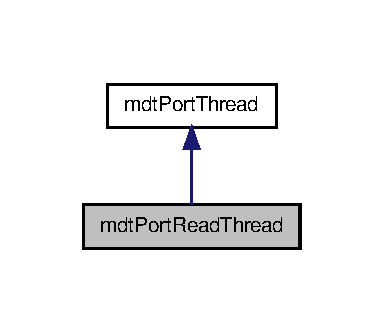
\includegraphics[width=184pt]{classmdt_port_read_thread__inherit__graph}
\end{center}
\end{figure}


Collaboration diagram for mdtPortReadThread:\nopagebreak
\begin{figure}[H]
\begin{center}
\leavevmode
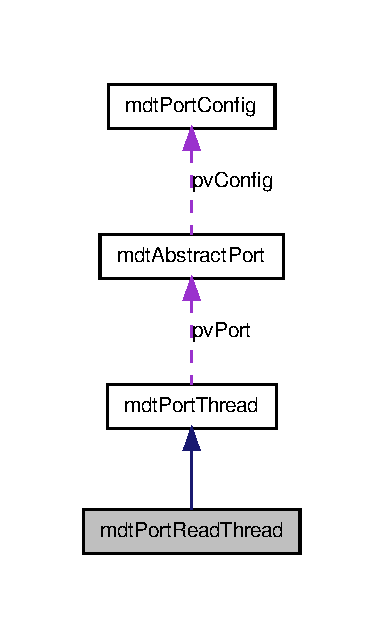
\includegraphics[width=184pt]{classmdt_port_read_thread__coll__graph}
\end{center}
\end{figure}
\subsection*{Public Member Functions}
\begin{DoxyCompactItemize}
\item 
\hypertarget{classmdt_port_read_thread_a180074c2ff60f5103d7e3aa27c1cdb01}{
{\bfseries mdtPortReadThread} (QObject $\ast$parent=0)}
\label{classmdt_port_read_thread_a180074c2ff60f5103d7e3aa27c1cdb01}

\item 
bool \hyperlink{classmdt_port_read_thread_a0138d613b61056c9f8373331de2d9a84}{isReader} () const 
\begin{DoxyCompactList}\small\item\em Returns true if this thread reads data and send the \hyperlink{classmdt_port_thread_a7fc2245c753fd65e1beffec211c41461}{newFrameReaden()} signal. \end{DoxyCompactList}\end{DoxyCompactItemize}


\subsection{Detailed Description}
Reader thread for port I/O. 

It's possible to use the read timeout protocol. An example of this is MODBUS (over serial line) in RTU mode.

\begin{DoxySeeAlso}{See also}
\hyperlink{classmdt_port_config}{mdtPortConfig}
\end{DoxySeeAlso}
\begin{Desc}
\item[\hyperlink{todo__todo000011}{Todo}]suspendTransmission() call is no longer in \hyperlink{classmdt_port_thread_a611211e56620ec9c699019452716e4fc}{getNewFrameRead()}, must be handled in run() now. \end{Desc}


Definition at line 37 of file mdtPortReadThread.h.



\subsection{Member Function Documentation}
\hypertarget{classmdt_port_read_thread_a0138d613b61056c9f8373331de2d9a84}{
\index{mdtPortReadThread@{mdtPortReadThread}!isReader@{isReader}}
\index{isReader@{isReader}!mdtPortReadThread@{mdtPortReadThread}}
\subsubsection[{isReader}]{\setlength{\rightskip}{0pt plus 5cm}bool mdtPortReadThread::isReader (
\begin{DoxyParamCaption}
{}
\end{DoxyParamCaption}
) const\hspace{0.3cm}{\ttfamily  \mbox{[}virtual\mbox{]}}}}
\label{classmdt_port_read_thread_a0138d613b61056c9f8373331de2d9a84}


Returns true if this thread reads data and send the \hyperlink{classmdt_port_thread_a7fc2245c753fd65e1beffec211c41461}{newFrameReaden()} signal. 

\hyperlink{classmdt_port_manager}{mdtPortManager} can handle many threads. It needs to know wich one will send the \hyperlink{classmdt_port_thread_a7fc2245c753fd65e1beffec211c41461}{newFrameReaden()} signal, so it can connect it to his slot. 

Implements \hyperlink{classmdt_port_thread_a3d57f15a864ae45c98eb40dd89f4cec6}{mdtPortThread}.



Definition at line 35 of file mdtPortReadThread.cpp.



The documentation for this class was generated from the following files:\begin{DoxyCompactItemize}
\item 
src/mdtport/mdtPortReadThread.h\item 
src/mdtport/mdtPortReadThread.cpp\end{DoxyCompactItemize}

\hypertarget{classmdt_port_term}{
\section{mdtPortTerm Class Reference}
\label{classmdt_port_term}\index{mdtPortTerm@{mdtPortTerm}}
}


Mini port treminal.  




{\ttfamily \#include $<$mdtPortTerm.h$>$}



Collaboration diagram for mdtPortTerm:\nopagebreak
\begin{figure}[H]
\begin{center}
\leavevmode
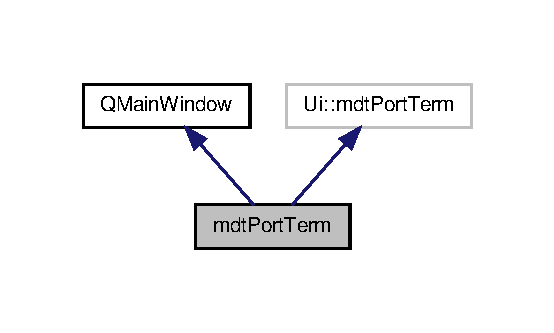
\includegraphics[width=400pt]{classmdt_port_term__coll__graph}
\end{center}
\end{figure}
\subsection*{Public Slots}
\begin{DoxyCompactItemize}
\item 
\hypertarget{classmdt_port_term_a2c8de2e82437fc94420ccb542cc42bf2}{
void \hyperlink{classmdt_port_term_a2c8de2e82437fc94420ccb542cc42bf2}{appendReadenData} (\hyperlink{classmdt_port_transaction}{mdtPortTransaction} $\ast$transaction)}
\label{classmdt_port_term_a2c8de2e82437fc94420ccb542cc42bf2}

\begin{DoxyCompactList}\small\item\em Append incomming data to terminal. \end{DoxyCompactList}\item 
\hypertarget{classmdt_port_term_a7ec568c44f862fe7aee83f1a271ac6bb}{
void \hyperlink{classmdt_port_term_a7ec568c44f862fe7aee83f1a271ac6bb}{sendCmd} ()}
\label{classmdt_port_term_a7ec568c44f862fe7aee83f1a271ac6bb}

\begin{DoxyCompactList}\small\item\em Send command to current port. \end{DoxyCompactList}\item 
\hypertarget{classmdt_port_term_a1b232e686b401d7103eb1c682be330a9}{
void \hyperlink{classmdt_port_term_a1b232e686b401d7103eb1c682be330a9}{on\_\-pbSendCmdAbort\_\-clicked} ()}
\label{classmdt_port_term_a1b232e686b401d7103eb1c682be330a9}

\begin{DoxyCompactList}\small\item\em Abort command transmission. \end{DoxyCompactList}\item 
\hypertarget{classmdt_port_term_abb3fc55837782dbea240b069a48b18ce}{
void \hyperlink{classmdt_port_term_abb3fc55837782dbea240b069a48b18ce}{on\_\-pbClearTerm\_\-clicked} ()}
\label{classmdt_port_term_abb3fc55837782dbea240b069a48b18ce}

\begin{DoxyCompactList}\small\item\em Clear terminal. \end{DoxyCompactList}\item 
void \hyperlink{classmdt_port_term_a542e20f789bcdc5f2ddf2b6e698ceea2}{retranslate} ()
\begin{DoxyCompactList}\small\item\em Retranslate. \end{DoxyCompactList}\end{DoxyCompactItemize}
\subsection*{Public Member Functions}
\begin{DoxyCompactItemize}
\item 
\hyperlink{classmdt_port_term_a5e93890f53b5112be80983779a3ab233}{mdtPortTerm} (QWidget $\ast$parent=0)
\item 
\hypertarget{classmdt_port_term_af6f97444089eb87ec5db557a2ccb24db}{
void \hyperlink{classmdt_port_term_af6f97444089eb87ec5db557a2ccb24db}{setAvailableTranslations} (const QMap$<$ QString, QString $>$ \&avaliableTranslations, const QString \&currentTranslationKey)}
\label{classmdt_port_term_af6f97444089eb87ec5db557a2ccb24db}

\begin{DoxyCompactList}\small\item\em Build the translations menu. \end{DoxyCompactList}\end{DoxyCompactItemize}


\subsection{Detailed Description}
Mini port treminal. 

Definition at line 44 of file mdtPortTerm.h.



\subsection{Constructor \& Destructor Documentation}
\hypertarget{classmdt_port_term_a5e93890f53b5112be80983779a3ab233}{
\index{mdtPortTerm@{mdtPortTerm}!mdtPortTerm@{mdtPortTerm}}
\index{mdtPortTerm@{mdtPortTerm}!mdtPortTerm@{mdtPortTerm}}
\subsubsection[{mdtPortTerm}]{\setlength{\rightskip}{0pt plus 5cm}mdtPortTerm::mdtPortTerm (
\begin{DoxyParamCaption}
\item[{QWidget $\ast$}]{parent = {\ttfamily 0}}
\end{DoxyParamCaption}
)}}
\label{classmdt_port_term_a5e93890f53b5112be80983779a3ab233}


action\_\-SerialPort-\/$>$setChecked(true); attachToSerialPort(); 



Definition at line 36 of file mdtPortTerm.cpp.



\subsection{Member Function Documentation}
\hypertarget{classmdt_port_term_a542e20f789bcdc5f2ddf2b6e698ceea2}{
\index{mdtPortTerm@{mdtPortTerm}!retranslate@{retranslate}}
\index{retranslate@{retranslate}!mdtPortTerm@{mdtPortTerm}}
\subsubsection[{retranslate}]{\setlength{\rightskip}{0pt plus 5cm}void mdtPortTerm::retranslate (
\begin{DoxyParamCaption}
{}
\end{DoxyParamCaption}
)\hspace{0.3cm}{\ttfamily  \mbox{[}slot\mbox{]}}}}
\label{classmdt_port_term_a542e20f789bcdc5f2ddf2b6e698ceea2}


Retranslate. 

This slot is called by \hyperlink{classmdt_application}{mdtApplication} when language has changed 

Definition at line 148 of file mdtPortTerm.cpp.



The documentation for this class was generated from the following files:\begin{DoxyCompactItemize}
\item 
src/mdttools/mdtPortTerm.h\item 
src/mdttools/mdtPortTerm.cpp\end{DoxyCompactItemize}

\hypertarget{classmdt_port_thread}{\section{mdt\-Port\-Thread Class Reference}
\label{classmdt_port_thread}\index{mdt\-Port\-Thread@{mdt\-Port\-Thread}}
}


{\ttfamily \#include $<$mdt\-Port\-Thread.\-h$>$}



Inheritance diagram for mdt\-Port\-Thread\-:\nopagebreak
\begin{figure}[H]
\begin{center}
\leavevmode
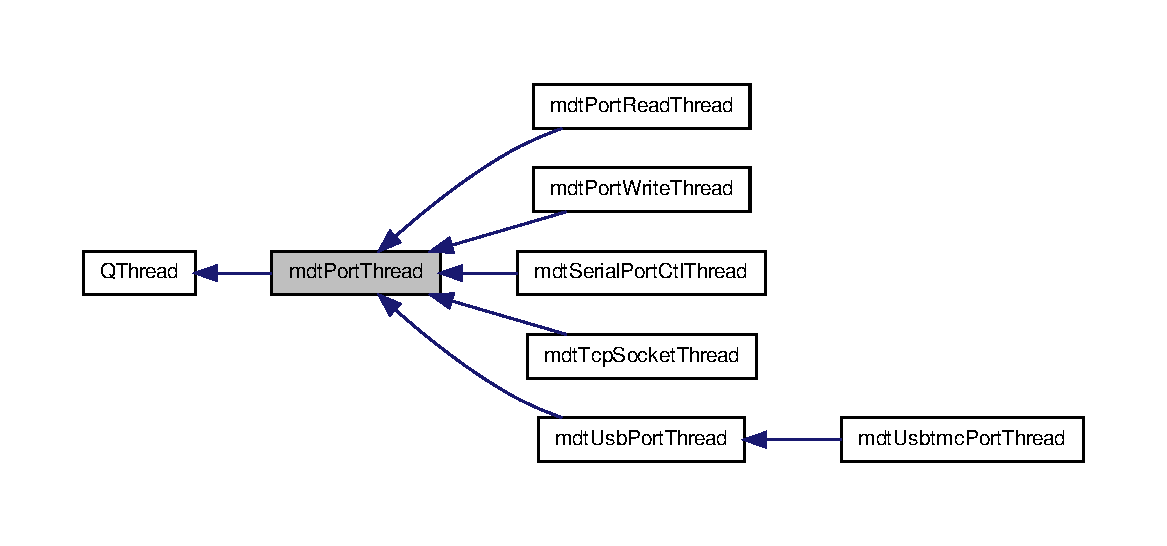
\includegraphics[width=350pt]{classmdt_port_thread__inherit__graph}
\end{center}
\end{figure}


Collaboration diagram for mdt\-Port\-Thread\-:\nopagebreak
\begin{figure}[H]
\begin{center}
\leavevmode
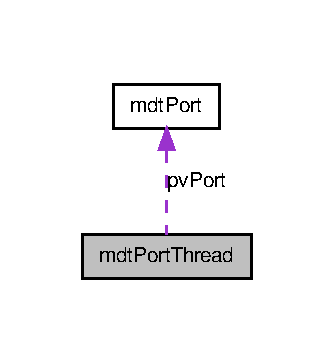
\includegraphics[width=350pt]{classmdt_port_thread__coll__graph}
\end{center}
\end{figure}
\subsection*{Signals}
\begin{DoxyCompactItemize}
\item 
void \hyperlink{classmdt_port_thread_abb7234a12814f5c7c98bd6c1c2ccb776}{read\-Process\-Begin} ()
\begin{DoxyCompactList}\small\item\em Emitted when a read process begins. \end{DoxyCompactList}\item 
void \hyperlink{classmdt_port_thread_aa01aac7e1a26deb823be40e6cb01b255}{write\-Process\-Begin} ()
\begin{DoxyCompactList}\small\item\em Emitted when a write process begins. \end{DoxyCompactList}\item 
void \hyperlink{classmdt_port_thread_a7fc2245c753fd65e1beffec211c41461}{new\-Frame\-Readen} ()
\begin{DoxyCompactList}\small\item\em Emited when a new frame is available. \end{DoxyCompactList}\item 
void \hyperlink{classmdt_port_thread_ab31cbe1a85aa830cd368654d1f806326}{error\-Occured} (int error)
\begin{DoxyCompactList}\small\item\em Emitted on error. \end{DoxyCompactList}\item 
void \hyperlink{classmdt_port_thread_ae71ae3aa58eb1f409a2b128e6ef3148b}{ready} (\hyperlink{classmdt_port_thread}{mdt\-Port\-Thread} $\ast$thread)
\begin{DoxyCompactList}\small\item\em Emitted when thread is started and ready. \end{DoxyCompactList}\item 
void \hyperlink{classmdt_port_thread_a4266192826f09d8186ee8f9b646ac089}{finished} (\hyperlink{classmdt_port_thread}{mdt\-Port\-Thread} $\ast$thread)
\begin{DoxyCompactList}\small\item\em Emitted when thread has finished executing. \end{DoxyCompactList}\item 
void \hyperlink{classmdt_port_thread_a88070ed43976a83b6e4d289d6f1827bd}{connected} ()
\begin{DoxyCompactList}\small\item\em Emitted when connection with device is done. \end{DoxyCompactList}\end{DoxyCompactItemize}
\subsection*{Public Member Functions}
\begin{DoxyCompactItemize}
\item 
\hyperlink{classmdt_port_thread_aa20869c68d7a016f9e547464f0d8b71e}{mdt\-Port\-Thread} (\hyperlink{class_q_object}{Q\-Object} $\ast$parent=0)
\item 
virtual \hyperlink{classmdt_port_thread_a554615870b4c3b18af73d2ab7262800d}{$\sim$mdt\-Port\-Thread} ()
\item 
virtual void \hyperlink{classmdt_port_thread_acd51474c3a2683676423317bc9cb31b2}{set\-Port} (\hyperlink{classmdt_abstract_port}{mdt\-Abstract\-Port} $\ast$\hyperlink{classmdt_port_thread_a97bff8cf6aca37d8858cc4e5c9294cae}{port})
\begin{DoxyCompactList}\small\item\em Set the port instance. \end{DoxyCompactList}\item 
\hyperlink{classmdt_abstract_port}{mdt\-Abstract\-Port} $\ast$ \hyperlink{classmdt_port_thread_a97bff8cf6aca37d8858cc4e5c9294cae}{port} ()
\begin{DoxyCompactList}\small\item\em Get port instance. \end{DoxyCompactList}\item 
virtual void \hyperlink{classmdt_port_thread_a29b434534a5564efbd9dfe570a61b143}{detach\-Port} (bool release\-Memory)
\begin{DoxyCompactList}\small\item\em Detach the port from thread. \end{DoxyCompactList}\item 
void \hyperlink{classmdt_port_thread_a5a5c1290eaa43182d69c3f39eadbec00}{start} ()
\begin{DoxyCompactList}\small\item\em Start the thread. \end{DoxyCompactList}\item 
virtual void \hyperlink{classmdt_port_thread_a5746ea96689ed80179751ad1353f0b39}{stop} ()
\begin{DoxyCompactList}\small\item\em Stop the running thread. \end{DoxyCompactList}\item 
void \hyperlink{classmdt_port_thread_aca7473f73c6b68fe8c3e1cfc349240e7}{wait\-Ready} ()
\begin{DoxyCompactList}\small\item\em Wait until thread is ready. \end{DoxyCompactList}\item 
void \hyperlink{classmdt_port_thread_a621c0748a16bc9ee15983ef488314c85}{wait\-Finished} ()
\begin{DoxyCompactList}\small\item\em Wait until thread is finished. \end{DoxyCompactList}\item 
bool \hyperlink{classmdt_port_thread_ae1becf17263dd9fbf5dfcc6c51eddd72}{is\-Running} () const 
\begin{DoxyCompactList}\small\item\em Returns true if the thread is running. \end{DoxyCompactList}\item 
void \hyperlink{classmdt_port_thread_ad9bcfaa66fba25512f2677a7e320c6c8}{set\-Running\-Flag} (bool running)
\begin{DoxyCompactList}\small\item\em Set the running flag. \end{DoxyCompactList}\item 
bool \hyperlink{classmdt_port_thread_abce96e61e09780841b729f28ab9054f0}{running\-Flag\-Set} () const 
\begin{DoxyCompactList}\small\item\em Get the running flag. \end{DoxyCompactList}\item 
bool \hyperlink{classmdt_port_thread_a55d7ef615447823bf9878492a2c88fd4}{is\-Finished} () const 
\begin{DoxyCompactList}\small\item\em Returns false if the thread is running. \end{DoxyCompactList}\item 
virtual bool \hyperlink{classmdt_port_thread_acdb3d96287c571cc08ef39860dc324b1}{is\-Reader} () const 
\begin{DoxyCompactList}\small\item\em Returns true if this thread reads data and send the \hyperlink{classmdt_port_thread_a7fc2245c753fd65e1beffec211c41461}{new\-Frame\-Readen()} signal. \end{DoxyCompactList}\item 
virtual bool \hyperlink{classmdt_port_thread_a0122a12262052cf3643241a3eaa31c58}{is\-Writer} () const 
\begin{DoxyCompactList}\small\item\em Returns true if this thread writes date. \end{DoxyCompactList}\item 
virtual bool \hyperlink{classmdt_port_thread_aaf671b84f7c1fb508ff9221dccee4c15}{handles\-Timeout} () const 
\begin{DoxyCompactList}\small\item\em Returns true is thread handles timeout(s) itself. \end{DoxyCompactList}\item 
void \hyperlink{classmdt_port_thread_a30bdd11ef16d4f3321921c9d9b26399d}{notify\-Error} (\hyperlink{classmdt_abstract_port_ad4121bb930c95887e77f8bafa065a85e}{mdt\-Abstract\-Port\-::error\-\_\-t} error, bool renotify\-Same\-Error=false)
\begin{DoxyCompactList}\small\item\em Emit the \hyperlink{classmdt_port_thread_ab31cbe1a85aa830cd368654d1f806326}{error\-Occured()} signal if new error is different from current. \end{DoxyCompactList}\item 
\hyperlink{classmdt_abstract_port_ad4121bb930c95887e77f8bafa065a85e}{mdt\-Abstract\-Port\-::error\-\_\-t} \hyperlink{classmdt_port_thread_adbc2d86162c23401e75184407b8c9428}{current\-Error} () const 
\begin{DoxyCompactList}\small\item\em Get current error. \end{DoxyCompactList}\end{DoxyCompactItemize}
\subsection*{Protected Member Functions}
\begin{DoxyCompactItemize}
\item 
\hyperlink{classmdt_abstract_port_ad4121bb930c95887e77f8bafa065a85e}{mdt\-Abstract\-Port\-::error\-\_\-t} \hyperlink{classmdt_port_thread_abee1d2f9b67ca37cfd13e108ca978b36}{reconnect} (bool notify=true)
\begin{DoxyCompactList}\small\item\em Try to reconnect to device/peer. \end{DoxyCompactList}\end{DoxyCompactItemize}
\subsection*{Static Protected Member Functions}
\begin{DoxyCompactItemize}
\item 
static void \hyperlink{classmdt_port_thread_a01d2362e0dfcece4cba242cb586d8d1c}{sigaction\-Handle} (int signum)
\end{DoxyCompactItemize}
\subsection*{Protected Attributes}
\begin{DoxyCompactItemize}
\item 
volatile bool \hyperlink{classmdt_port_thread_a59735ef01b761361b1055a0356be525a}{pv\-Running}
\item 
\hyperlink{classmdt_abstract_port}{mdt\-Abstract\-Port} $\ast$ \hyperlink{classmdt_port_thread_af5c4bed0c9fb012f220fba013d0f69b8}{pv\-Port}
\item 
pthread\-\_\-t \hyperlink{classmdt_port_thread_a7154af7d387eecaea113ddb5900ff23c}{pv\-Native\-Pthread\-Object}
\item 
struct sigaction \hyperlink{classmdt_port_thread_ae22f83fd56b06cdaa9b77abafe85a6b4}{pv\-Sigaction}
\end{DoxyCompactItemize}


\subsection{Detailed Description}


Definition at line 36 of file mdt\-Port\-Thread.\-h.



\subsection{Constructor \& Destructor Documentation}
\hypertarget{classmdt_port_thread_aa20869c68d7a016f9e547464f0d8b71e}{\index{mdt\-Port\-Thread@{mdt\-Port\-Thread}!mdt\-Port\-Thread@{mdt\-Port\-Thread}}
\index{mdt\-Port\-Thread@{mdt\-Port\-Thread}!mdtPortThread@{mdt\-Port\-Thread}}
\subsubsection[{mdt\-Port\-Thread}]{\setlength{\rightskip}{0pt plus 5cm}mdt\-Port\-Thread\-::mdt\-Port\-Thread (
\begin{DoxyParamCaption}
\item[{{\bf Q\-Object} $\ast$}]{parent = {\ttfamily 0}}
\end{DoxyParamCaption}
)}}\label{classmdt_port_thread_aa20869c68d7a016f9e547464f0d8b71e}


Definition at line 30 of file mdt\-Port\-Thread.\-cpp.



References finished(), pv\-Native\-Pthread\-Object, pv\-Port, pv\-Running, pv\-Sigaction, sigaction\-Handle(), and mdt\-Abstract\-Port\-::\-Unhandled\-Error.

\hypertarget{classmdt_port_thread_a554615870b4c3b18af73d2ab7262800d}{\index{mdt\-Port\-Thread@{mdt\-Port\-Thread}!$\sim$mdt\-Port\-Thread@{$\sim$mdt\-Port\-Thread}}
\index{$\sim$mdt\-Port\-Thread@{$\sim$mdt\-Port\-Thread}!mdtPortThread@{mdt\-Port\-Thread}}
\subsubsection[{$\sim$mdt\-Port\-Thread}]{\setlength{\rightskip}{0pt plus 5cm}mdt\-Port\-Thread\-::$\sim$mdt\-Port\-Thread (
\begin{DoxyParamCaption}
{}
\end{DoxyParamCaption}
)\hspace{0.3cm}{\ttfamily [virtual]}}}\label{classmdt_port_thread_a554615870b4c3b18af73d2ab7262800d}


Definition at line 50 of file mdt\-Port\-Thread.\-cpp.



References is\-Running(), and stop().



\subsection{Member Function Documentation}
\hypertarget{classmdt_port_thread_a88070ed43976a83b6e4d289d6f1827bd}{\index{mdt\-Port\-Thread@{mdt\-Port\-Thread}!connected@{connected}}
\index{connected@{connected}!mdtPortThread@{mdt\-Port\-Thread}}
\subsubsection[{connected}]{\setlength{\rightskip}{0pt plus 5cm}void mdt\-Port\-Thread\-::connected (
\begin{DoxyParamCaption}
{}
\end{DoxyParamCaption}
)\hspace{0.3cm}{\ttfamily [signal]}}}\label{classmdt_port_thread_a88070ed43976a83b6e4d289d6f1827bd}


Emitted when connection with device is done. 

Notes\-:
\begin{DoxyItemize}
\item Disconnection, connection, etc... are notified as error
\item Some threads does not send this signal, because device connection is not handled directly by port protocol. 
\end{DoxyItemize}

Referenced by reconnect().

\hypertarget{classmdt_port_thread_adbc2d86162c23401e75184407b8c9428}{\index{mdt\-Port\-Thread@{mdt\-Port\-Thread}!current\-Error@{current\-Error}}
\index{current\-Error@{current\-Error}!mdtPortThread@{mdt\-Port\-Thread}}
\subsubsection[{current\-Error}]{\setlength{\rightskip}{0pt plus 5cm}{\bf mdt\-Abstract\-Port\-::error\-\_\-t} mdt\-Port\-Thread\-::current\-Error (
\begin{DoxyParamCaption}
{}
\end{DoxyParamCaption}
) const}}\label{classmdt_port_thread_adbc2d86162c23401e75184407b8c9428}


Get current error. 

This is used by \hyperlink{classmdt_port_manager}{mdt\-Port\-Manager}.

Port's mutex is not handled by this method. 

Definition at line 225 of file mdt\-Port\-Thread.\-cpp.

\hypertarget{classmdt_port_thread_a29b434534a5564efbd9dfe570a61b143}{\index{mdt\-Port\-Thread@{mdt\-Port\-Thread}!detach\-Port@{detach\-Port}}
\index{detach\-Port@{detach\-Port}!mdtPortThread@{mdt\-Port\-Thread}}
\subsubsection[{detach\-Port}]{\setlength{\rightskip}{0pt plus 5cm}void mdt\-Port\-Thread\-::detach\-Port (
\begin{DoxyParamCaption}
\item[{bool}]{release\-Memory}
\end{DoxyParamCaption}
)\hspace{0.3cm}{\ttfamily [virtual]}}}\label{classmdt_port_thread_a29b434534a5564efbd9dfe570a61b143}


Detach the port from thread. 


\begin{DoxyParams}{Parameters}
{\em release\-Memory} & If true, the port object that was set with \hyperlink{classmdt_port_thread_acd51474c3a2683676423317bc9cb31b2}{set\-Port()} will be deleted. \\
\hline
\end{DoxyParams}
\begin{DoxyPrecond}{Precondition}
The thread must not running 
\end{DoxyPrecond}


Reimplemented in \hyperlink{classmdt_usb_port_thread_a99070e7dba4bd7939b054cddbd66979f}{mdt\-Usb\-Port\-Thread}.



Definition at line 70 of file mdt\-Port\-Thread.\-cpp.



References pv\-Port.



Referenced by mdt\-Usb\-Port\-Thread\-::detach\-Port().

\hypertarget{classmdt_port_thread_ab31cbe1a85aa830cd368654d1f806326}{\index{mdt\-Port\-Thread@{mdt\-Port\-Thread}!error\-Occured@{error\-Occured}}
\index{error\-Occured@{error\-Occured}!mdtPortThread@{mdt\-Port\-Thread}}
\subsubsection[{error\-Occured}]{\setlength{\rightskip}{0pt plus 5cm}void mdt\-Port\-Thread\-::error\-Occured (
\begin{DoxyParamCaption}
\item[{int}]{error}
\end{DoxyParamCaption}
)\hspace{0.3cm}{\ttfamily [signal]}}}\label{classmdt_port_thread_ab31cbe1a85aa830cd368654d1f806326}


Emitted on error. 

\begin{DoxyRefDesc}{Todo}
\item[\hyperlink{todo__todo000031}{Todo}]Adapt threads + port managers\end{DoxyRefDesc}


When a error occurs, this signal is emited.

The error is one of the \hyperlink{classmdt_abstract_port_ad4121bb930c95887e77f8bafa065a85e}{mdt\-Abstract\-Port\-::error\-\_\-t}.

\hyperlink{classmdt_port_manager}{mdt\-Port\-Manager} uses this signal. 

Referenced by notify\-Error().

\hypertarget{classmdt_port_thread_a4266192826f09d8186ee8f9b646ac089}{\index{mdt\-Port\-Thread@{mdt\-Port\-Thread}!finished@{finished}}
\index{finished@{finished}!mdtPortThread@{mdt\-Port\-Thread}}
\subsubsection[{finished}]{\setlength{\rightskip}{0pt plus 5cm}void mdt\-Port\-Thread\-::finished (
\begin{DoxyParamCaption}
\item[{{\bf mdt\-Port\-Thread} $\ast$}]{thread}
\end{DoxyParamCaption}
)\hspace{0.3cm}{\ttfamily [signal]}}}\label{classmdt_port_thread_a4266192826f09d8186ee8f9b646ac089}


Emitted when thread has finished executing. 



Referenced by mdt\-Port\-Thread().

\hypertarget{classmdt_port_thread_aaf671b84f7c1fb508ff9221dccee4c15}{\index{mdt\-Port\-Thread@{mdt\-Port\-Thread}!handles\-Timeout@{handles\-Timeout}}
\index{handles\-Timeout@{handles\-Timeout}!mdtPortThread@{mdt\-Port\-Thread}}
\subsubsection[{handles\-Timeout}]{\setlength{\rightskip}{0pt plus 5cm}bool mdt\-Port\-Thread\-::handles\-Timeout (
\begin{DoxyParamCaption}
{}
\end{DoxyParamCaption}
) const\hspace{0.3cm}{\ttfamily [virtual]}}}\label{classmdt_port_thread_aaf671b84f7c1fb508ff9221dccee4c15}


Returns true is thread handles timeout(s) itself. 

For example, \hyperlink{classmdt_usb_port_thread}{mdt\-Usb\-Port\-Thread} and subclasses handles timeout itself. \hyperlink{classmdt_port_read_thread}{mdt\-Port\-Read\-Thread} does not.

\hyperlink{classmdt_port_manager}{mdt\-Port\-Manager} uses this flag to know how to deal with timeouts.

This implementation returns false. 

Reimplemented in \hyperlink{classmdt_usb_port_thread_aeaa2dabc53e57f6b7cf7077d113c7f40}{mdt\-Usb\-Port\-Thread}, \hyperlink{classmdt_port_read_thread_afa42f86f3fed878b8f44cacb3a2f41af}{mdt\-Port\-Read\-Thread}, and \hyperlink{classmdt_tcp_socket_thread_aa14c9838dfb8d2defac449b8b58bbc7c}{mdt\-Tcp\-Socket\-Thread}.



Definition at line 211 of file mdt\-Port\-Thread.\-cpp.



Referenced by mdt\-Port\-Manager\-::add\-Thread().

\hypertarget{classmdt_port_thread_a55d7ef615447823bf9878492a2c88fd4}{\index{mdt\-Port\-Thread@{mdt\-Port\-Thread}!is\-Finished@{is\-Finished}}
\index{is\-Finished@{is\-Finished}!mdtPortThread@{mdt\-Port\-Thread}}
\subsubsection[{is\-Finished}]{\setlength{\rightskip}{0pt plus 5cm}bool mdt\-Port\-Thread\-::is\-Finished (
\begin{DoxyParamCaption}
{}
\end{DoxyParamCaption}
) const}}\label{classmdt_port_thread_a55d7ef615447823bf9878492a2c88fd4}


Returns false if the thread is running. 

\begin{DoxySeeAlso}{See Also}
\hyperlink{classmdt_port_thread_ae1becf17263dd9fbf5dfcc6c51eddd72}{is\-Running()} 
\end{DoxySeeAlso}


Definition at line 185 of file mdt\-Port\-Thread.\-cpp.



References mdt\-Abstract\-Port\-::lock\-Mutex(), pv\-Port, pv\-Running, and mdt\-Abstract\-Port\-::unlock\-Mutex().



Referenced by wait\-Finished().

\hypertarget{classmdt_port_thread_acdb3d96287c571cc08ef39860dc324b1}{\index{mdt\-Port\-Thread@{mdt\-Port\-Thread}!is\-Reader@{is\-Reader}}
\index{is\-Reader@{is\-Reader}!mdtPortThread@{mdt\-Port\-Thread}}
\subsubsection[{is\-Reader}]{\setlength{\rightskip}{0pt plus 5cm}bool mdt\-Port\-Thread\-::is\-Reader (
\begin{DoxyParamCaption}
{}
\end{DoxyParamCaption}
) const\hspace{0.3cm}{\ttfamily [virtual]}}}\label{classmdt_port_thread_acdb3d96287c571cc08ef39860dc324b1}


Returns true if this thread reads data and send the \hyperlink{classmdt_port_thread_a7fc2245c753fd65e1beffec211c41461}{new\-Frame\-Readen()} signal. 

\hyperlink{classmdt_port_manager}{mdt\-Port\-Manager} can handle many threads. It needs to know wich one will send the \hyperlink{classmdt_port_thread_a7fc2245c753fd65e1beffec211c41461}{new\-Frame\-Readen()} signal, so it can connect it to his slot.

Default implementation returns allways false.

This method should be implemented in reader subclass. 

Reimplemented in \hyperlink{classmdt_usb_port_thread_aed82b57c84745f1e2391750697db1022}{mdt\-Usb\-Port\-Thread}, \hyperlink{classmdt_port_read_thread_a0138d613b61056c9f8373331de2d9a84}{mdt\-Port\-Read\-Thread}, \hyperlink{classmdt_usbtmc_port_thread_a27c115427b49d5ae988c9f9c9a5e402a}{mdt\-Usbtmc\-Port\-Thread}, \hyperlink{classmdt_port_write_thread_ac37bb988773f624def51e841998a2f1e}{mdt\-Port\-Write\-Thread}, \hyperlink{classmdt_tcp_socket_thread_a3224f12c8ff8d695975030f3f6215010}{mdt\-Tcp\-Socket\-Thread}, and \hyperlink{classmdt_serial_port_ctl_thread_ab87413cedc8d0540eac553e55a3f6407}{mdt\-Serial\-Port\-Ctl\-Thread}.



Definition at line 201 of file mdt\-Port\-Thread.\-cpp.



Referenced by mdt\-Port\-Manager\-::add\-Thread(), and mdt\-Port\-Manager\-::remove\-Threads().

\hypertarget{classmdt_port_thread_ae1becf17263dd9fbf5dfcc6c51eddd72}{\index{mdt\-Port\-Thread@{mdt\-Port\-Thread}!is\-Running@{is\-Running}}
\index{is\-Running@{is\-Running}!mdtPortThread@{mdt\-Port\-Thread}}
\subsubsection[{is\-Running}]{\setlength{\rightskip}{0pt plus 5cm}bool mdt\-Port\-Thread\-::is\-Running (
\begin{DoxyParamCaption}
{}
\end{DoxyParamCaption}
) const}}\label{classmdt_port_thread_ae1becf17263dd9fbf5dfcc6c51eddd72}


Returns true if the thread is running. 

This function overloads the Q\-Thread\-::is\-Running() function. Note for subclass\-: when the thread is started and ready, the private member pv\-Running must be set to true. 

Definition at line 157 of file mdt\-Port\-Thread.\-cpp.



References mdt\-Abstract\-Port\-::lock\-Mutex(), pv\-Port, pv\-Running, and mdt\-Abstract\-Port\-::unlock\-Mutex().



Referenced by wait\-Ready(), and $\sim$mdt\-Port\-Thread().

\hypertarget{classmdt_port_thread_a0122a12262052cf3643241a3eaa31c58}{\index{mdt\-Port\-Thread@{mdt\-Port\-Thread}!is\-Writer@{is\-Writer}}
\index{is\-Writer@{is\-Writer}!mdtPortThread@{mdt\-Port\-Thread}}
\subsubsection[{is\-Writer}]{\setlength{\rightskip}{0pt plus 5cm}bool mdt\-Port\-Thread\-::is\-Writer (
\begin{DoxyParamCaption}
{}
\end{DoxyParamCaption}
) const\hspace{0.3cm}{\ttfamily [virtual]}}}\label{classmdt_port_thread_a0122a12262052cf3643241a3eaa31c58}


Returns true if this thread writes date. 

Is used by \hyperlink{classmdt_port_thread_a5746ea96689ed80179751ad1353f0b39}{mdt\-Port\-Thread\-::stop()} to know if \hyperlink{classmdt_abstract_port_ae67c815f68317c70e398eaa86622af6b}{mdt\-Abstract\-Port\-::abort\-Frame\-To\-Write\-Wait()} must be called.

Default implementation returns false 

Reimplemented in \hyperlink{classmdt_usb_port_thread_a74258f300967b5dea1fbfa9a0ccab38a}{mdt\-Usb\-Port\-Thread}, \hyperlink{classmdt_usbtmc_port_thread_a4c58b7140f0483a19723b14487907423}{mdt\-Usbtmc\-Port\-Thread}, \hyperlink{classmdt_port_write_thread_ad2508c3a2433383e2de705e9f3d2e602}{mdt\-Port\-Write\-Thread}, and \hyperlink{classmdt_tcp_socket_thread_a014ad2b3a5fbe7031eeb1d42d8f0767d}{mdt\-Tcp\-Socket\-Thread}.



Definition at line 206 of file mdt\-Port\-Thread.\-cpp.



Referenced by mdt\-Port\-Manager\-::add\-Thread(), and stop().

\hypertarget{classmdt_port_thread_a7fc2245c753fd65e1beffec211c41461}{\index{mdt\-Port\-Thread@{mdt\-Port\-Thread}!new\-Frame\-Readen@{new\-Frame\-Readen}}
\index{new\-Frame\-Readen@{new\-Frame\-Readen}!mdtPortThread@{mdt\-Port\-Thread}}
\subsubsection[{new\-Frame\-Readen}]{\setlength{\rightskip}{0pt plus 5cm}void mdt\-Port\-Thread\-::new\-Frame\-Readen (
\begin{DoxyParamCaption}
{}
\end{DoxyParamCaption}
)\hspace{0.3cm}{\ttfamily [signal]}}}\label{classmdt_port_thread_a7fc2245c753fd65e1beffec211c41461}


Emited when a new frame is available. 

This signal is emited when a new frame is available.

To get the frame, the simplest way is to use a \hyperlink{classmdt_port_manager}{mdt\-Port\-Manager}.

It's also possible to use \hyperlink{classmdt_port}{mdt\-Port}, but this solution needs to handle the mutex, verify the readen queue state, ...

\begin{DoxySeeAlso}{See Also}
\hyperlink{classmdt_port_manager}{mdt\-Port\-Manager} 

\hyperlink{classmdt_port}{mdt\-Port} 
\end{DoxySeeAlso}
\hypertarget{classmdt_port_thread_a30bdd11ef16d4f3321921c9d9b26399d}{\index{mdt\-Port\-Thread@{mdt\-Port\-Thread}!notify\-Error@{notify\-Error}}
\index{notify\-Error@{notify\-Error}!mdtPortThread@{mdt\-Port\-Thread}}
\subsubsection[{notify\-Error}]{\setlength{\rightskip}{0pt plus 5cm}void mdt\-Port\-Thread\-::notify\-Error (
\begin{DoxyParamCaption}
\item[{{\bf mdt\-Abstract\-Port\-::error\-\_\-t}}]{error, }
\item[{bool}]{renotify\-Same\-Error = {\ttfamily false}}
\end{DoxyParamCaption}
)}}\label{classmdt_port_thread_a30bdd11ef16d4f3321921c9d9b26399d}


Emit the \hyperlink{classmdt_port_thread_ab31cbe1a85aa830cd368654d1f806326}{error\-Occured()} signal if new error is different from current. 


\begin{DoxyParams}{Parameters}
{\em renotify\-Same\-Error} & For some cases, the same error must be notified each time it happens. If this flag is true, signal is emitted without checking previous error. \\
\hline
\end{DoxyParams}


Definition at line 216 of file mdt\-Port\-Thread.\-cpp.



References error\-Occured().



Referenced by mdt\-Port\-Thread\-Helper\-::notify\-Error(), and reconnect().

\hypertarget{classmdt_port_thread_a97bff8cf6aca37d8858cc4e5c9294cae}{\index{mdt\-Port\-Thread@{mdt\-Port\-Thread}!port@{port}}
\index{port@{port}!mdtPortThread@{mdt\-Port\-Thread}}
\subsubsection[{port}]{\setlength{\rightskip}{0pt plus 5cm}{\bf mdt\-Abstract\-Port} $\ast$ mdt\-Port\-Thread\-::port (
\begin{DoxyParamCaption}
{}
\end{DoxyParamCaption}
)}}\label{classmdt_port_thread_a97bff8cf6aca37d8858cc4e5c9294cae}


Get port instance. 

\begin{DoxyReturn}{Returns}
Port instance, or a null pointer if it was not set 
\end{DoxyReturn}


Definition at line 65 of file mdt\-Port\-Thread.\-cpp.



References pv\-Port.



Referenced by set\-Port(), and mdt\-Usb\-Port\-Thread\-::set\-Port().

\hypertarget{classmdt_port_thread_abb7234a12814f5c7c98bd6c1c2ccb776}{\index{mdt\-Port\-Thread@{mdt\-Port\-Thread}!read\-Process\-Begin@{read\-Process\-Begin}}
\index{read\-Process\-Begin@{read\-Process\-Begin}!mdtPortThread@{mdt\-Port\-Thread}}
\subsubsection[{read\-Process\-Begin}]{\setlength{\rightskip}{0pt plus 5cm}void mdt\-Port\-Thread\-::read\-Process\-Begin (
\begin{DoxyParamCaption}
{}
\end{DoxyParamCaption}
)\hspace{0.3cm}{\ttfamily [signal]}}}\label{classmdt_port_thread_abb7234a12814f5c7c98bd6c1c2ccb776}


Emitted when a read process begins. 

This can be used to display read state. Please consider that this signal is emitted each time the read process begins, and not when it ends. This is because asynch I/\-O calls are fast, and nothing will be seen from user if we update state before/after I/\-O call. To handle this, use this signal as trigger, and hold the state some stime (f.\-ex. 100 \mbox{[}ms\mbox{]}) \hypertarget{classmdt_port_thread_ae71ae3aa58eb1f409a2b128e6ef3148b}{\index{mdt\-Port\-Thread@{mdt\-Port\-Thread}!ready@{ready}}
\index{ready@{ready}!mdtPortThread@{mdt\-Port\-Thread}}
\subsubsection[{ready}]{\setlength{\rightskip}{0pt plus 5cm}void mdt\-Port\-Thread\-::ready (
\begin{DoxyParamCaption}
\item[{{\bf mdt\-Port\-Thread} $\ast$}]{thread}
\end{DoxyParamCaption}
)\hspace{0.3cm}{\ttfamily [signal]}}}\label{classmdt_port_thread_ae71ae3aa58eb1f409a2b128e6ef3148b}


Emitted when thread is started and ready. 

\hypertarget{classmdt_port_thread_abee1d2f9b67ca37cfd13e108ca978b36}{\index{mdt\-Port\-Thread@{mdt\-Port\-Thread}!reconnect@{reconnect}}
\index{reconnect@{reconnect}!mdtPortThread@{mdt\-Port\-Thread}}
\subsubsection[{reconnect}]{\setlength{\rightskip}{0pt plus 5cm}{\bf mdt\-Abstract\-Port\-::error\-\_\-t} mdt\-Port\-Thread\-::reconnect (
\begin{DoxyParamCaption}
\item[{bool}]{notify = {\ttfamily true}}
\end{DoxyParamCaption}
)\hspace{0.3cm}{\ttfamily [protected]}}}\label{classmdt_port_thread_abee1d2f9b67ca37cfd13e108ca978b36}


Try to reconnect to device/peer. 

This is a helper method for subclass. When a port method returns a Disconnected error, the thread can call this method, wich will try to reconnect (using \hyperlink{classmdt_abstract_port_aec74b2db1a629d98a95d8f042ea96653}{mdt\-Abstract\-Port\-::reconnect()} ) until max retry was reached.

Reconnect timeout and max try are readen from port config, in \hyperlink{classmdt_port_thread_a5a5c1290eaa43182d69c3f39eadbec00}{start()} method.


\begin{DoxyParams}{Parameters}
{\em notify} & If true, error will be notified (with \hyperlink{classmdt_port_thread_ab31cbe1a85aa830cd368654d1f806326}{error\-Occured()} ), and failure after max\-Try will be reported with \hyperlink{classmdt_error}{mdt\-Error}. \\
\hline
\end{DoxyParams}
\begin{DoxyReturn}{Returns}
No\-Error if reconnection worked or Unhandled\-Error else.
\end{DoxyReturn}
\begin{DoxyPrecond}{Precondition}
Port must be set with \hyperlink{classmdt_port_thread_acd51474c3a2683676423317bc9cb31b2}{set\-Port()} before using this method. 
\end{DoxyPrecond}


Definition at line 230 of file mdt\-Port\-Thread.\-cpp.



References mdt\-Error\-::commit(), connected(), mdt\-Abstract\-Port\-::\-Connecting, mdt\-Abstract\-Port\-::\-Connection\-Failed, mdt\-Abstract\-Port\-::\-Disconnected, mdt\-Error\-::\-Error, M\-D\-T\-\_\-\-E\-R\-R\-O\-R\-\_\-\-S\-E\-T\-\_\-\-S\-R\-C, M\-D\-T\-\_\-\-P\-O\-R\-T\-\_\-\-I\-O\-\_\-\-E\-R\-R\-O\-R, mdt\-Abstract\-Port\-::\-No\-Error, notify\-Error(), pv\-Port, pv\-Running, mdt\-Abstract\-Port\-::reconnect(), mdt\-Abstract\-Port\-::\-Unhandled\-Error, and mdt\-Error\-::\-Warning.

\hypertarget{classmdt_port_thread_abce96e61e09780841b729f28ab9054f0}{\index{mdt\-Port\-Thread@{mdt\-Port\-Thread}!running\-Flag\-Set@{running\-Flag\-Set}}
\index{running\-Flag\-Set@{running\-Flag\-Set}!mdtPortThread@{mdt\-Port\-Thread}}
\subsubsection[{running\-Flag\-Set}]{\setlength{\rightskip}{0pt plus 5cm}bool mdt\-Port\-Thread\-::running\-Flag\-Set (
\begin{DoxyParamCaption}
{}
\end{DoxyParamCaption}
) const}}\label{classmdt_port_thread_abce96e61e09780841b729f28ab9054f0}


Get the running flag. 

This method is used by \hyperlink{classmdt_port_thread_helper}{mdt\-Port\-Thread\-Helper} and should not be used directly.

Port's mutex is not handled in this method. 

Definition at line 180 of file mdt\-Port\-Thread.\-cpp.



References pv\-Running.



Referenced by mdt\-Port\-Thread\-Helper\-::get\-New\-Frame\-Read(), mdt\-Port\-Thread\-Helper\-::get\-New\-Frame\-Write(), mdt\-Port\-Thread\-Helper\-::handle\-Common\-Read\-Errors(), mdt\-Port\-Thread\-Helper\-::handle\-Common\-Write\-Errors(), and mdt\-Port\-Thread\-Helper\-Port\-::write\-To\-Port().

\hypertarget{classmdt_port_thread_acd51474c3a2683676423317bc9cb31b2}{\index{mdt\-Port\-Thread@{mdt\-Port\-Thread}!set\-Port@{set\-Port}}
\index{set\-Port@{set\-Port}!mdtPortThread@{mdt\-Port\-Thread}}
\subsubsection[{set\-Port}]{\setlength{\rightskip}{0pt plus 5cm}void mdt\-Port\-Thread\-::set\-Port (
\begin{DoxyParamCaption}
\item[{{\bf mdt\-Abstract\-Port} $\ast$}]{port}
\end{DoxyParamCaption}
)\hspace{0.3cm}{\ttfamily [virtual]}}}\label{classmdt_port_thread_acd51474c3a2683676423317bc9cb31b2}


Set the port instance. 

\begin{DoxyPrecond}{Precondition}
port must be a valid pointer 

The thread must not running 
\end{DoxyPrecond}


Definition at line 57 of file mdt\-Port\-Thread.\-cpp.



References port(), and pv\-Port.



Referenced by mdt\-Port\-Manager\-::add\-Thread(), and mdt\-Usb\-Port\-Thread\-::set\-Port().

\hypertarget{classmdt_port_thread_ad9bcfaa66fba25512f2677a7e320c6c8}{\index{mdt\-Port\-Thread@{mdt\-Port\-Thread}!set\-Running\-Flag@{set\-Running\-Flag}}
\index{set\-Running\-Flag@{set\-Running\-Flag}!mdtPortThread@{mdt\-Port\-Thread}}
\subsubsection[{set\-Running\-Flag}]{\setlength{\rightskip}{0pt plus 5cm}void mdt\-Port\-Thread\-::set\-Running\-Flag (
\begin{DoxyParamCaption}
\item[{bool}]{running}
\end{DoxyParamCaption}
)}}\label{classmdt_port_thread_ad9bcfaa66fba25512f2677a7e320c6c8}


Set the running flag. 

This method is used by \hyperlink{classmdt_port_thread_helper}{mdt\-Port\-Thread\-Helper} and should not be used directly.

Port's mutex is not handled in this method. 

Definition at line 175 of file mdt\-Port\-Thread.\-cpp.



References pv\-Running.

\hypertarget{classmdt_port_thread_a01d2362e0dfcece4cba242cb586d8d1c}{\index{mdt\-Port\-Thread@{mdt\-Port\-Thread}!sigaction\-Handle@{sigaction\-Handle}}
\index{sigaction\-Handle@{sigaction\-Handle}!mdtPortThread@{mdt\-Port\-Thread}}
\subsubsection[{sigaction\-Handle}]{\setlength{\rightskip}{0pt plus 5cm}void mdt\-Port\-Thread\-::sigaction\-Handle (
\begin{DoxyParamCaption}
\item[{int}]{signum}
\end{DoxyParamCaption}
)\hspace{0.3cm}{\ttfamily [static]}, {\ttfamily [protected]}}}\label{classmdt_port_thread_a01d2362e0dfcece4cba242cb586d8d1c}


Definition at line 281 of file mdt\-Port\-Thread.\-cpp.



Referenced by mdt\-Port\-Thread().

\hypertarget{classmdt_port_thread_a5a5c1290eaa43182d69c3f39eadbec00}{\index{mdt\-Port\-Thread@{mdt\-Port\-Thread}!start@{start}}
\index{start@{start}!mdtPortThread@{mdt\-Port\-Thread}}
\subsubsection[{start}]{\setlength{\rightskip}{0pt plus 5cm}void mdt\-Port\-Thread\-::start (
\begin{DoxyParamCaption}
{}
\end{DoxyParamCaption}
)}}\label{classmdt_port_thread_a5a5c1290eaa43182d69c3f39eadbec00}


Start the thread. 

This method will not wait until thread is running and ready. Once thread is ready, \hyperlink{classmdt_port_thread_ae71ae3aa58eb1f409a2b128e6ef3148b}{ready()} signal is emitted.

\begin{DoxyPrecond}{Precondition}
Port instance must be defined. 

Port must have a valid configuration. 
\end{DoxyPrecond}


Definition at line 80 of file mdt\-Port\-Thread.\-cpp.



References mdt\-Abstract\-Port\-::config(), mdt\-Port\-Config\-::connect\-Max\-Try(), mdt\-Port\-Config\-::connect\-Timeout(), pv\-Port, and mdt\-Abstract\-Port\-::\-Unhandled\-Error.

\hypertarget{classmdt_port_thread_a5746ea96689ed80179751ad1353f0b39}{\index{mdt\-Port\-Thread@{mdt\-Port\-Thread}!stop@{stop}}
\index{stop@{stop}!mdtPortThread@{mdt\-Port\-Thread}}
\subsubsection[{stop}]{\setlength{\rightskip}{0pt plus 5cm}void mdt\-Port\-Thread\-::stop (
\begin{DoxyParamCaption}
{}
\end{DoxyParamCaption}
)\hspace{0.3cm}{\ttfamily [virtual]}}}\label{classmdt_port_thread_a5746ea96689ed80179751ad1353f0b39}


Stop the running thread. 

This method will not wait until thread is stopped. Once thread is stopped, \hyperlink{classmdt_port_thread_a4266192826f09d8186ee8f9b646ac089}{finished()} signal is emitted.

\begin{DoxyPrecond}{Precondition}
Port instance must be defined with \hyperlink{classmdt_port_thread_acd51474c3a2683676423317bc9cb31b2}{set\-Port()}. 
\end{DoxyPrecond}


Reimplemented in \hyperlink{classmdt_port_write_thread_a69702ab3a95c238fb451f866efc7cb34}{mdt\-Port\-Write\-Thread}.



Definition at line 92 of file mdt\-Port\-Thread.\-cpp.



References mdt\-Abstract\-Port\-::abort\-Frame\-To\-Write\-Wait(), mdt\-Error\-::commit(), mdt\-Error\-::\-Error, is\-Writer(), mdt\-Abstract\-Port\-::lock\-Mutex(), M\-D\-T\-\_\-\-E\-R\-R\-O\-R\-\_\-\-S\-E\-T\-\_\-\-S\-R\-C, M\-D\-T\-\_\-\-P\-O\-R\-T\-\_\-\-I\-O\-\_\-\-E\-R\-R\-O\-R, pv\-Native\-Pthread\-Object, pv\-Port, pv\-Running, mdt\-Error\-::set\-System\-Error(), mdt\-Abstract\-Port\-::\-Unhandled\-Error, and mdt\-Abstract\-Port\-::unlock\-Mutex().



Referenced by mdt\-Port\-Write\-Thread\-::stop(), and $\sim$mdt\-Port\-Thread().

\hypertarget{classmdt_port_thread_a621c0748a16bc9ee15983ef488314c85}{\index{mdt\-Port\-Thread@{mdt\-Port\-Thread}!wait\-Finished@{wait\-Finished}}
\index{wait\-Finished@{wait\-Finished}!mdtPortThread@{mdt\-Port\-Thread}}
\subsubsection[{wait\-Finished}]{\setlength{\rightskip}{0pt plus 5cm}void mdt\-Port\-Thread\-::wait\-Finished (
\begin{DoxyParamCaption}
{}
\end{DoxyParamCaption}
)}}\label{classmdt_port_thread_a621c0748a16bc9ee15983ef488314c85}


Wait until thread is finished. 

This is a conveniance method, mainly used by test suite. Port manager, for example, use the finished signal ensteatd of this method. 

Definition at line 148 of file mdt\-Port\-Thread.\-cpp.



References is\-Finished(), and msleep.

\hypertarget{classmdt_port_thread_aca7473f73c6b68fe8c3e1cfc349240e7}{\index{mdt\-Port\-Thread@{mdt\-Port\-Thread}!wait\-Ready@{wait\-Ready}}
\index{wait\-Ready@{wait\-Ready}!mdtPortThread@{mdt\-Port\-Thread}}
\subsubsection[{wait\-Ready}]{\setlength{\rightskip}{0pt plus 5cm}void mdt\-Port\-Thread\-::wait\-Ready (
\begin{DoxyParamCaption}
{}
\end{DoxyParamCaption}
)}}\label{classmdt_port_thread_aca7473f73c6b68fe8c3e1cfc349240e7}


Wait until thread is ready. 

This is a conveniance method, mainly used by test suite. Port manager, for example, use the ready signal ensteatd of this method. 

Definition at line 139 of file mdt\-Port\-Thread.\-cpp.



References is\-Running(), and msleep.

\hypertarget{classmdt_port_thread_aa01aac7e1a26deb823be40e6cb01b255}{\index{mdt\-Port\-Thread@{mdt\-Port\-Thread}!write\-Process\-Begin@{write\-Process\-Begin}}
\index{write\-Process\-Begin@{write\-Process\-Begin}!mdtPortThread@{mdt\-Port\-Thread}}
\subsubsection[{write\-Process\-Begin}]{\setlength{\rightskip}{0pt plus 5cm}void mdt\-Port\-Thread\-::write\-Process\-Begin (
\begin{DoxyParamCaption}
{}
\end{DoxyParamCaption}
)\hspace{0.3cm}{\ttfamily [signal]}}}\label{classmdt_port_thread_aa01aac7e1a26deb823be40e6cb01b255}


Emitted when a write process begins. 

This can be used to display write state. Please consider that this signal is emitted each time the write process begins, and not when it ends. This is because asynch I/\-O calls are fast, and nothing will be seen from user if we update state before/after I/\-O call. To handle this, use this signal as trigger, and hold the state some stime (f.\-ex. 100 \mbox{[}ms\mbox{]}) 

\subsection{Member Data Documentation}
\hypertarget{classmdt_port_thread_a7154af7d387eecaea113ddb5900ff23c}{\index{mdt\-Port\-Thread@{mdt\-Port\-Thread}!pv\-Native\-Pthread\-Object@{pv\-Native\-Pthread\-Object}}
\index{pv\-Native\-Pthread\-Object@{pv\-Native\-Pthread\-Object}!mdtPortThread@{mdt\-Port\-Thread}}
\subsubsection[{pv\-Native\-Pthread\-Object}]{\setlength{\rightskip}{0pt plus 5cm}pthread\-\_\-t mdt\-Port\-Thread\-::pv\-Native\-Pthread\-Object\hspace{0.3cm}{\ttfamily [protected]}}}\label{classmdt_port_thread_a7154af7d387eecaea113ddb5900ff23c}


Definition at line 270 of file mdt\-Port\-Thread.\-h.



Referenced by mdt\-Port\-Thread(), and stop().

\hypertarget{classmdt_port_thread_af5c4bed0c9fb012f220fba013d0f69b8}{\index{mdt\-Port\-Thread@{mdt\-Port\-Thread}!pv\-Port@{pv\-Port}}
\index{pv\-Port@{pv\-Port}!mdtPortThread@{mdt\-Port\-Thread}}
\subsubsection[{pv\-Port}]{\setlength{\rightskip}{0pt plus 5cm}{\bf mdt\-Abstract\-Port}$\ast$ mdt\-Port\-Thread\-::pv\-Port\hspace{0.3cm}{\ttfamily [protected]}}}\label{classmdt_port_thread_af5c4bed0c9fb012f220fba013d0f69b8}


Definition at line 264 of file mdt\-Port\-Thread.\-h.



Referenced by detach\-Port(), is\-Finished(), is\-Running(), mdt\-Port\-Thread(), port(), reconnect(), set\-Port(), start(), mdt\-Port\-Write\-Thread\-::stop(), and stop().

\hypertarget{classmdt_port_thread_a59735ef01b761361b1055a0356be525a}{\index{mdt\-Port\-Thread@{mdt\-Port\-Thread}!pv\-Running@{pv\-Running}}
\index{pv\-Running@{pv\-Running}!mdtPortThread@{mdt\-Port\-Thread}}
\subsubsection[{pv\-Running}]{\setlength{\rightskip}{0pt plus 5cm}volatile bool mdt\-Port\-Thread\-::pv\-Running\hspace{0.3cm}{\ttfamily [protected]}}}\label{classmdt_port_thread_a59735ef01b761361b1055a0356be525a}


Definition at line 263 of file mdt\-Port\-Thread.\-h.



Referenced by is\-Finished(), is\-Running(), mdt\-Port\-Thread(), reconnect(), running\-Flag\-Set(), mdt\-Usb\-Port\-Thread\-::send\-Control\-Query(), set\-Running\-Flag(), stop(), and mdt\-Usb\-Port\-Thread\-::wait\-On\-Control\-Transfer\-Possible().

\hypertarget{classmdt_port_thread_ae22f83fd56b06cdaa9b77abafe85a6b4}{\index{mdt\-Port\-Thread@{mdt\-Port\-Thread}!pv\-Sigaction@{pv\-Sigaction}}
\index{pv\-Sigaction@{pv\-Sigaction}!mdtPortThread@{mdt\-Port\-Thread}}
\subsubsection[{pv\-Sigaction}]{\setlength{\rightskip}{0pt plus 5cm}struct sigaction mdt\-Port\-Thread\-::pv\-Sigaction\hspace{0.3cm}{\ttfamily [protected]}}}\label{classmdt_port_thread_ae22f83fd56b06cdaa9b77abafe85a6b4}


Definition at line 271 of file mdt\-Port\-Thread.\-h.



Referenced by mdt\-Port\-Thread().



The documentation for this class was generated from the following files\-:\begin{DoxyCompactItemize}
\item 
src/mdtport/\hyperlink{mdt_port_thread_8h}{mdt\-Port\-Thread.\-h}\item 
src/mdtport/\hyperlink{mdt_port_thread_8cpp}{mdt\-Port\-Thread.\-cpp}\end{DoxyCompactItemize}

\hypertarget{classmdt_port_write_thread}{
\section{mdtPortWriteThread Class Reference}
\label{classmdt_port_write_thread}\index{mdtPortWriteThread@{mdtPortWriteThread}}
}


Inheritance diagram for mdtPortWriteThread:\nopagebreak
\begin{figure}[H]
\begin{center}
\leavevmode
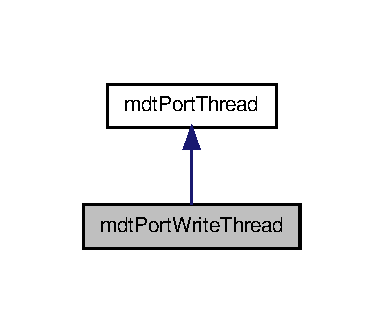
\includegraphics[width=184pt]{classmdt_port_write_thread__inherit__graph}
\end{center}
\end{figure}


Collaboration diagram for mdtPortWriteThread:\nopagebreak
\begin{figure}[H]
\begin{center}
\leavevmode
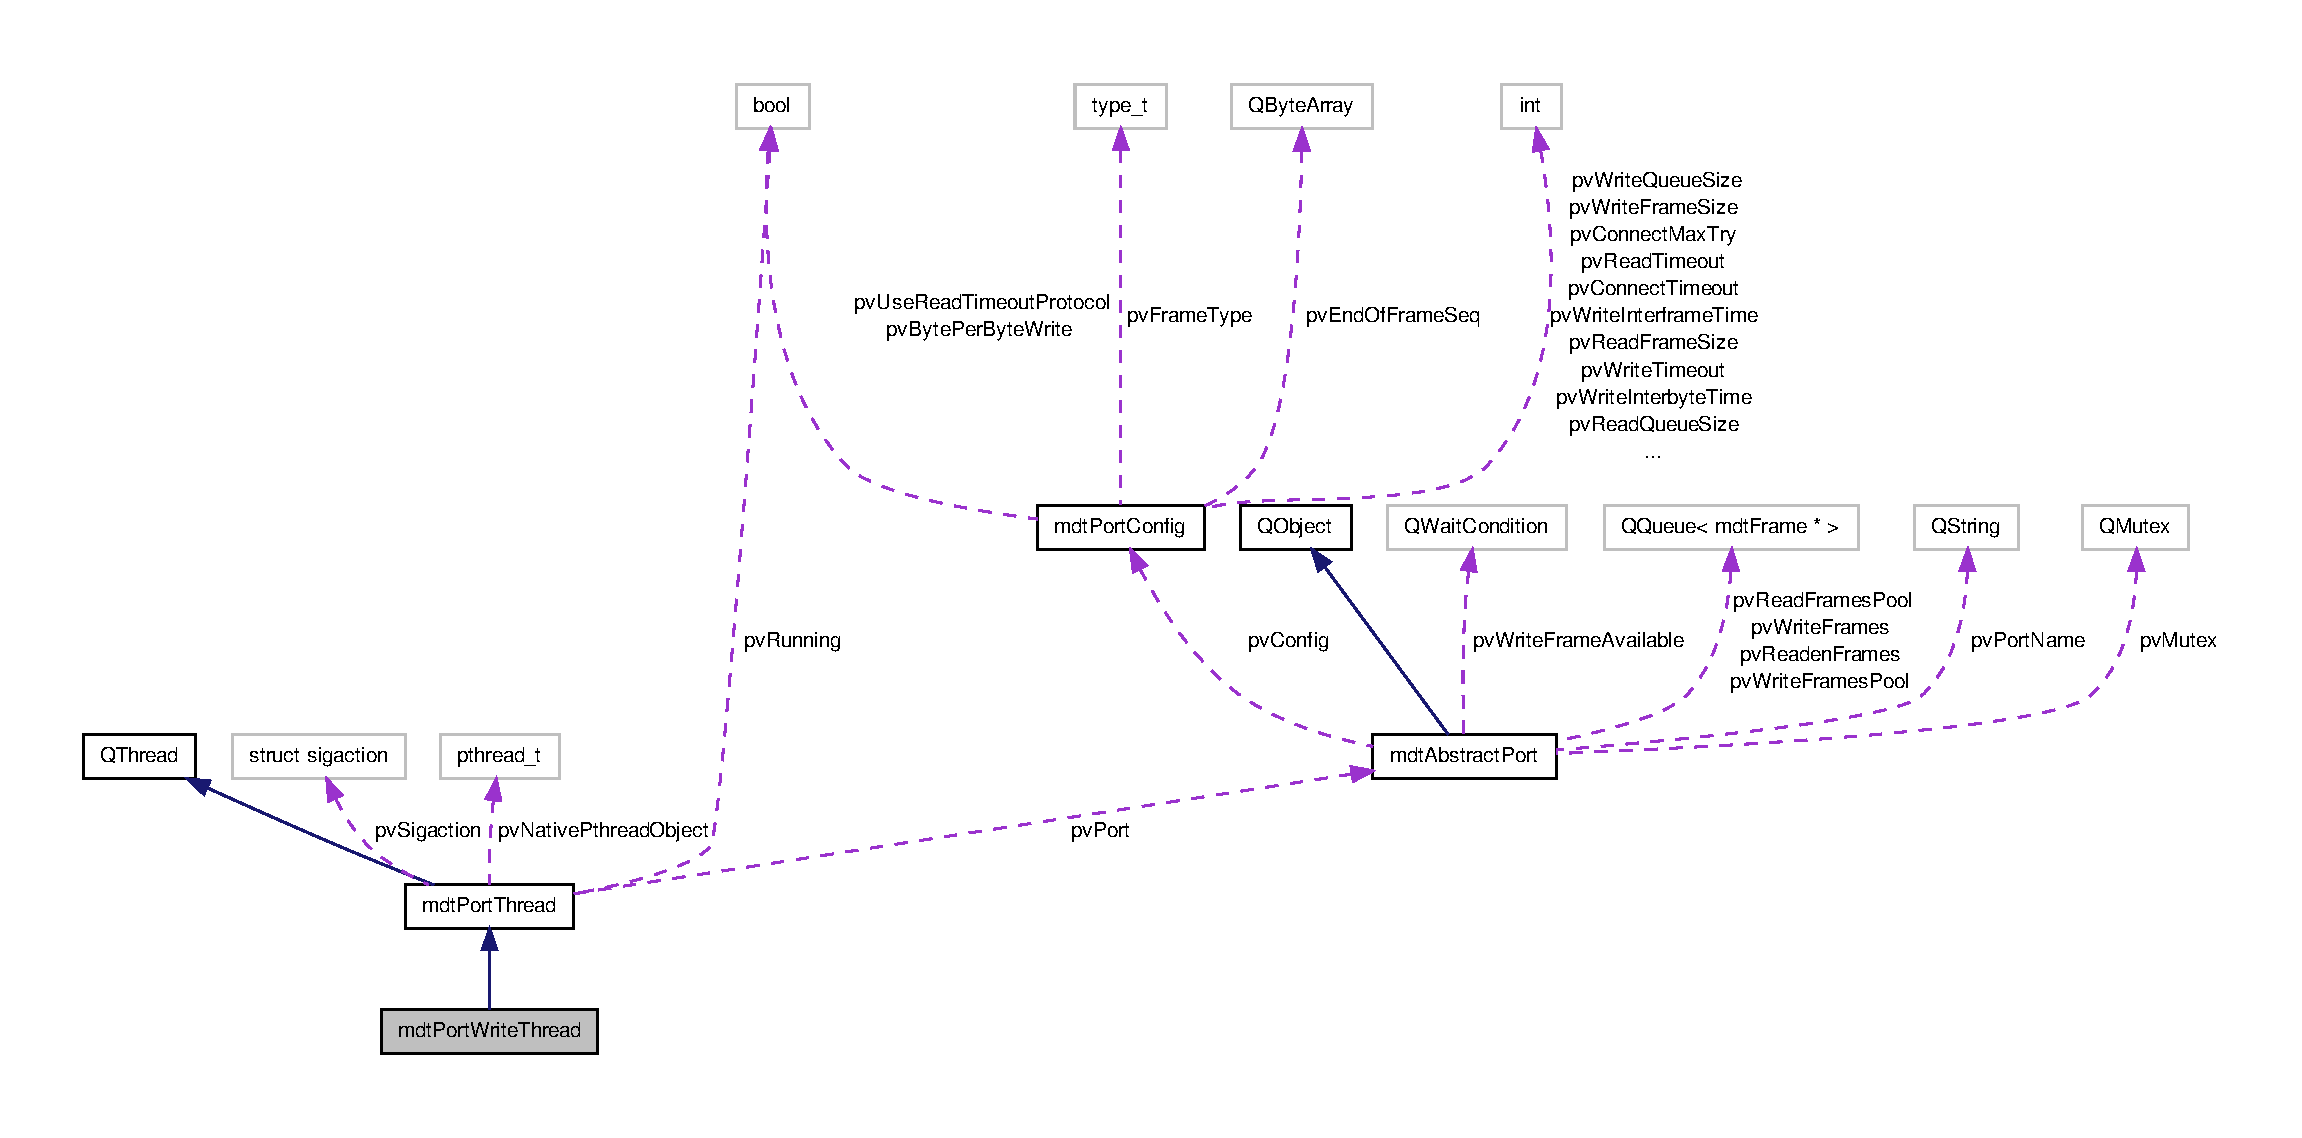
\includegraphics[width=184pt]{classmdt_port_write_thread__coll__graph}
\end{center}
\end{figure}
\subsection*{Signals}
\begin{DoxyCompactItemize}
\item 
void \hyperlink{classmdt_port_write_thread_a8ea77f140d6d4f6fa731dbb80acf5da6}{frameWritten} ()
\begin{DoxyCompactList}\small\item\em Emited when a complete frame was written. \end{DoxyCompactList}\end{DoxyCompactItemize}
\subsection*{Public Member Functions}
\begin{DoxyCompactItemize}
\item 
\hypertarget{classmdt_port_write_thread_a994b96eafdd721ccff2f2410a5abd5e3}{
{\bfseries mdtPortWriteThread} (QObject $\ast$parent=0)}
\label{classmdt_port_write_thread_a994b96eafdd721ccff2f2410a5abd5e3}

\end{DoxyCompactItemize}


\subsection{Member Function Documentation}
\hypertarget{classmdt_port_write_thread_a8ea77f140d6d4f6fa731dbb80acf5da6}{
\index{mdtPortWriteThread@{mdtPortWriteThread}!frameWritten@{frameWritten}}
\index{frameWritten@{frameWritten}!mdtPortWriteThread@{mdtPortWriteThread}}
\subsubsection[{frameWritten}]{\setlength{\rightskip}{0pt plus 5cm}void mdtPortWriteThread::frameWritten (
\begin{DoxyParamCaption}
{}
\end{DoxyParamCaption}
)\hspace{0.3cm}{\ttfamily  \mbox{[}signal\mbox{]}}}}
\label{classmdt_port_write_thread_a8ea77f140d6d4f6fa731dbb80acf5da6}


Emited when a complete frame was written. 

\begin{DoxySeeAlso}{See also}
\hyperlink{classmdt_port_manager}{mdtPortManager} 

\hyperlink{classmdt_port}{mdtPort} 
\end{DoxySeeAlso}


The documentation for this class was generated from the following files:\begin{DoxyCompactItemize}
\item 
src/mdtutils/mdtPortWriteThread.h\item 
src/mdtutils/mdtPortWriteThread.cpp\item 
src/mdtutils/moc\_\-mdtPortWriteThread.cxx\end{DoxyCompactItemize}

\hypertarget{classmdt_serial_port}{\section{mdt\-Serial\-Port Class Reference}
\label{classmdt_serial_port}\index{mdt\-Serial\-Port@{mdt\-Serial\-Port}}
}


{\ttfamily \#include $<$mdt\-Serial\-Port.\-h$>$}



Inheritance diagram for mdt\-Serial\-Port\-:\nopagebreak
\begin{figure}[H]
\begin{center}
\leavevmode
\includegraphics[width=192pt]{classmdt_serial_port__inherit__graph}
\end{center}
\end{figure}


Collaboration diagram for mdt\-Serial\-Port\-:\nopagebreak
\begin{figure}[H]
\begin{center}
\leavevmode
\includegraphics[width=350pt]{classmdt_serial_port__coll__graph}
\end{center}
\end{figure}
\subsection*{Public Member Functions}
\begin{DoxyCompactItemize}
\item 
\hyperlink{classmdt_serial_port_a7b2da083885e727981c1fd4414634cae}{mdt\-Serial\-Port} (\hyperlink{class_q_object}{Q\-Object} $\ast$parent=0)
\item 
\hyperlink{classmdt_serial_port_a7149994f7b5eac8a13cfe57b465e1901}{$\sim$mdt\-Serial\-Port} ()
\item 
bool \hyperlink{classmdt_serial_port_ad77b6a5fd819fae6db0db888b3113351}{set\-Baud\-Rate} (int rate)
\begin{DoxyCompactList}\small\item\em Set the baud rate. \end{DoxyCompactList}\item 
int \hyperlink{classmdt_serial_port_ab7d9433433f4ec5d5e584721e5bb1195}{baud\-Rate} ()
\begin{DoxyCompactList}\small\item\em Get the baud rate. \end{DoxyCompactList}\item 
bool \hyperlink{classmdt_serial_port_af39774b2d3c4121623253740660a0389}{set\-Data\-Bits} (int n)
\begin{DoxyCompactList}\small\item\em Set number of data bits. \end{DoxyCompactList}\item 
int \hyperlink{classmdt_serial_port_a65c92bdb5543c1fe0034169ffc88d09f}{data\-Bits} ()
\begin{DoxyCompactList}\small\item\em Get number of data bits. \end{DoxyCompactList}\item 
bool \hyperlink{classmdt_serial_port_a9471ebff90de41decee977566dd1571f}{set\-Stop\-Bits} (int n)
\begin{DoxyCompactList}\small\item\em Set number of stop bits. \end{DoxyCompactList}\item 
int \hyperlink{classmdt_serial_port_a163a83bdcac2c81a5c6b097c4afde41f}{stop\-Bits} ()
\begin{DoxyCompactList}\small\item\em Get number of stop bits. \end{DoxyCompactList}\item 
bool \hyperlink{classmdt_serial_port_ae435f052a87dcd0b1829f1577bb5e58d}{set\-Parity} (\hyperlink{classmdt_serial_port_config_a4b9e444637cf0193a125fabdd67d8bfe}{mdt\-Serial\-Port\-Config\-::parity\-\_\-t} p)
\begin{DoxyCompactList}\small\item\em Set parity check. \end{DoxyCompactList}\item 
\hyperlink{classmdt_serial_port_config_a4b9e444637cf0193a125fabdd67d8bfe}{mdt\-Serial\-Port\-Config\-::parity\-\_\-t} \hyperlink{classmdt_serial_port_a98938e2c51d1888236b920903f99050a}{parity} ()
\begin{DoxyCompactList}\small\item\em Get configured parity. \end{DoxyCompactList}\item 
bool \hyperlink{classmdt_serial_port_a175785be0dfe124254484822b7b8832e}{set\-Flow\-Ctl\-Rts\-Cts} (bool on)
\begin{DoxyCompactList}\small\item\em Enable/diseable R\-T\-S/\-C\-T\-S flow control. \end{DoxyCompactList}\item 
bool \hyperlink{classmdt_serial_port_a9315ed0c7854a09716a4585efb0094c7}{flow\-Ctl\-Rts\-Cts\-On} ()
\begin{DoxyCompactList}\small\item\em Get configured state of R\-T\-S/\-C\-T\-S flow control. \end{DoxyCompactList}\item 
bool \hyperlink{classmdt_serial_port_a34e2ac7b0d3cb7a6fb65756cbca2ce48}{set\-Flow\-Ctl\-Xon\-Xoff} (bool on, char xon\-Char, char xoff\-Char)
\begin{DoxyCompactList}\small\item\em Enable/diseable Xon/\-Xoff flow control. \end{DoxyCompactList}\item 
bool \hyperlink{classmdt_serial_port_a8d3e3eb1d2272129b8b97377dff1d5d4}{flow\-Ctl\-Xon\-Xoff\-On} ()
\begin{DoxyCompactList}\small\item\em Get configured state of Xon/\-Xoff flow control. \end{DoxyCompactList}\item 
void \hyperlink{classmdt_serial_port_a9105e5a3a640b56097c1156000ace933}{set\-Read\-Timeout} (int timeout)
\begin{DoxyCompactList}\small\item\em Set the read data timeout. \end{DoxyCompactList}\item 
void \hyperlink{classmdt_serial_port_a036f49d743838013c9a8cbf6a1dd40d1}{set\-Write\-Timeout} (int timeout)
\begin{DoxyCompactList}\small\item\em Set the write data timeout. \end{DoxyCompactList}\item 
\hyperlink{classmdt_abstract_port_ad4121bb930c95887e77f8bafa065a85e}{error\-\_\-t} \hyperlink{classmdt_serial_port_ad150a45c68d98a501bea2f102aeadb50}{wait\-For\-Ready\-Read} ()
\begin{DoxyCompactList}\small\item\em Wait until data is available on port. \end{DoxyCompactList}\item 
qint64 \hyperlink{classmdt_serial_port_a12274d7956b2af961ccdd36cfc2052cc}{read} (char $\ast$data, qint64 max\-Size)
\begin{DoxyCompactList}\small\item\em Read data from port. \end{DoxyCompactList}\item 
bool \hyperlink{classmdt_serial_port_a9412faf413eca5ee3516139fdfaaf2fe}{suspend\-Transmission} ()
\begin{DoxyCompactList}\small\item\em Request to suspend transmission. \end{DoxyCompactList}\item 
bool \hyperlink{classmdt_serial_port_a02fd5ee74a7f52c3bce0545ec8a659bf}{resume\-Transmission} ()
\begin{DoxyCompactList}\small\item\em Request to resume transmission. \end{DoxyCompactList}\item 
\hyperlink{classmdt_abstract_port_ad4121bb930c95887e77f8bafa065a85e}{error\-\_\-t} \hyperlink{classmdt_serial_port_a988825b3ff2ef93a1b43e2df316055bd}{wait\-Event\-Write\-Ready} ()
\begin{DoxyCompactList}\small\item\em void \hyperlink{classmdt_abstract_port_a32329b4188db796401e4f454755acb44}{flush\-In()}; \end{DoxyCompactList}\item 
qint64 \hyperlink{classmdt_serial_port_a282f99035c032fbb6fa86ccd10deb597}{write} (const char $\ast$data, qint64 max\-Size)
\begin{DoxyCompactList}\small\item\em Write data to port. \end{DoxyCompactList}\item 
\hyperlink{classmdt_abstract_port_ad4121bb930c95887e77f8bafa065a85e}{error\-\_\-t} \hyperlink{classmdt_serial_port_a9d1402c229401343a3bf66eeda4fe9da}{wait\-Event\-Ctl} ()
\begin{DoxyCompactList}\small\item\em void \hyperlink{classmdt_abstract_port_ad199c6310801893f1f7de2a2391606fc}{flush\-Out()}; \end{DoxyCompactList}\item 
bool \hyperlink{classmdt_serial_port_a7893e1817fe5fc59c77ee6f3b9f13ae7}{get\-Ctl\-States} ()
\begin{DoxyCompactList}\small\item\em N\-O\-T\-E\-: \end{DoxyCompactList}\item 
void \hyperlink{classmdt_serial_port_af0534e9f2e25b44a1a127d2a34b409fb}{set\-Rts} (bool on)
\begin{DoxyCompactList}\small\item\em Enable/diseable the R\-T\-S (Request To Send) signal. \end{DoxyCompactList}\item 
void \hyperlink{classmdt_serial_port_a91ec8a600f09b6844d36902fe1e16592}{set\-Dtr} (bool on)
\begin{DoxyCompactList}\small\item\em Enable/diseable the D\-T\-R (Data Terminal Ready) signal. \end{DoxyCompactList}\end{DoxyCompactItemize}
\subsection*{Additional Inherited Members}


\subsection{Detailed Description}


Definition at line 40 of file mdt\-Serial\-Port.\-h.



\subsection{Constructor \& Destructor Documentation}
\hypertarget{classmdt_serial_port_a7b2da083885e727981c1fd4414634cae}{\index{mdt\-Serial\-Port@{mdt\-Serial\-Port}!mdt\-Serial\-Port@{mdt\-Serial\-Port}}
\index{mdt\-Serial\-Port@{mdt\-Serial\-Port}!mdtSerialPort@{mdt\-Serial\-Port}}
\subsubsection[{mdt\-Serial\-Port}]{\setlength{\rightskip}{0pt plus 5cm}mdt\-Serial\-Port\-::mdt\-Serial\-Port (
\begin{DoxyParamCaption}
\item[{{\bf Q\-Object} $\ast$}]{parent = {\ttfamily 0}}
\end{DoxyParamCaption}
)}}\label{classmdt_serial_port_a7b2da083885e727981c1fd4414634cae}


Definition at line 35 of file mdt\-Serial\-Port.\-cpp.

\hypertarget{classmdt_serial_port_a7149994f7b5eac8a13cfe57b465e1901}{\index{mdt\-Serial\-Port@{mdt\-Serial\-Port}!$\sim$mdt\-Serial\-Port@{$\sim$mdt\-Serial\-Port}}
\index{$\sim$mdt\-Serial\-Port@{$\sim$mdt\-Serial\-Port}!mdtSerialPort@{mdt\-Serial\-Port}}
\subsubsection[{$\sim$mdt\-Serial\-Port}]{\setlength{\rightskip}{0pt plus 5cm}mdt\-Serial\-Port\-::$\sim$mdt\-Serial\-Port (
\begin{DoxyParamCaption}
{}
\end{DoxyParamCaption}
)}}\label{classmdt_serial_port_a7149994f7b5eac8a13cfe57b465e1901}


Definition at line 47 of file mdt\-Serial\-Port.\-cpp.



References mdt\-Abstract\-Serial\-Port\-::close().



\subsection{Member Function Documentation}
\hypertarget{classmdt_serial_port_ab7d9433433f4ec5d5e584721e5bb1195}{\index{mdt\-Serial\-Port@{mdt\-Serial\-Port}!baud\-Rate@{baud\-Rate}}
\index{baud\-Rate@{baud\-Rate}!mdtSerialPort@{mdt\-Serial\-Port}}
\subsubsection[{baud\-Rate}]{\setlength{\rightskip}{0pt plus 5cm}int mdt\-Serial\-Port\-::baud\-Rate (
\begin{DoxyParamCaption}
{}
\end{DoxyParamCaption}
)\hspace{0.3cm}{\ttfamily [virtual]}}}\label{classmdt_serial_port_ab7d9433433f4ec5d5e584721e5bb1195}


Get the baud rate. 

The mutex is not handled by this method.

\begin{DoxyReturn}{Returns}
Configured baud rate, or 0 on error. 
\end{DoxyReturn}


Implements \hyperlink{classmdt_abstract_serial_port_ad9f5b7e939c60cd3766d2bf76df4af4b}{mdt\-Abstract\-Serial\-Port}.



Definition at line 210 of file mdt\-Serial\-Port.\-cpp.



References mdt\-Error\-::commit(), mdt\-Error\-::\-Error, M\-D\-T\-\_\-\-E\-R\-R\-O\-R\-\_\-\-S\-E\-T\-\_\-\-S\-R\-C, M\-D\-T\-\_\-\-S\-E\-R\-I\-A\-L\-\_\-\-P\-O\-R\-T\-\_\-\-I\-O\-\_\-\-E\-R\-R\-O\-R, and mdt\-Error\-::set\-System\-Error().



Referenced by set\-Baud\-Rate().

\hypertarget{classmdt_serial_port_a65c92bdb5543c1fe0034169ffc88d09f}{\index{mdt\-Serial\-Port@{mdt\-Serial\-Port}!data\-Bits@{data\-Bits}}
\index{data\-Bits@{data\-Bits}!mdtSerialPort@{mdt\-Serial\-Port}}
\subsubsection[{data\-Bits}]{\setlength{\rightskip}{0pt plus 5cm}int mdt\-Serial\-Port\-::data\-Bits (
\begin{DoxyParamCaption}
{}
\end{DoxyParamCaption}
)\hspace{0.3cm}{\ttfamily [virtual]}}}\label{classmdt_serial_port_a65c92bdb5543c1fe0034169ffc88d09f}


Get number of data bits. 

The mutex is not handled by this method.

\begin{DoxyReturn}{Returns}
Configured data bits count or 0 on error. 
\end{DoxyReturn}


Implements \hyperlink{classmdt_abstract_serial_port_a63e2a14c416d9c3516ec74f5e37f4cc7}{mdt\-Abstract\-Serial\-Port}.



Definition at line 400 of file mdt\-Serial\-Port.\-cpp.



References mdt\-Error\-::commit(), mdt\-Error\-::\-Error, M\-D\-T\-\_\-\-E\-R\-R\-O\-R\-\_\-\-S\-E\-T\-\_\-\-S\-R\-C, M\-D\-T\-\_\-\-S\-E\-R\-I\-A\-L\-\_\-\-P\-O\-R\-T\-\_\-\-I\-O\-\_\-\-E\-R\-R\-O\-R, and mdt\-Error\-::set\-System\-Error().



Referenced by set\-Data\-Bits().

\hypertarget{classmdt_serial_port_a9315ed0c7854a09716a4585efb0094c7}{\index{mdt\-Serial\-Port@{mdt\-Serial\-Port}!flow\-Ctl\-Rts\-Cts\-On@{flow\-Ctl\-Rts\-Cts\-On}}
\index{flow\-Ctl\-Rts\-Cts\-On@{flow\-Ctl\-Rts\-Cts\-On}!mdtSerialPort@{mdt\-Serial\-Port}}
\subsubsection[{flow\-Ctl\-Rts\-Cts\-On}]{\setlength{\rightskip}{0pt plus 5cm}bool mdt\-Serial\-Port\-::flow\-Ctl\-Rts\-Cts\-On (
\begin{DoxyParamCaption}
{}
\end{DoxyParamCaption}
)\hspace{0.3cm}{\ttfamily [virtual]}}}\label{classmdt_serial_port_a9315ed0c7854a09716a4585efb0094c7}


Get configured state of R\-T\-S/\-C\-T\-S flow control. 

The mutex is not handled by this method.

\begin{DoxyReturn}{Returns}
True if R\-T\-S/\-C\-T\-S flow control is enabled (and no error occured). 
\end{DoxyReturn}


Implements \hyperlink{classmdt_abstract_serial_port_a7a1163b4d44d80369bd56c65af7942ad}{mdt\-Abstract\-Serial\-Port}.



Definition at line 543 of file mdt\-Serial\-Port.\-cpp.



References mdt\-Error\-::commit(), mdt\-Error\-::\-Error, M\-D\-T\-\_\-\-E\-R\-R\-O\-R\-\_\-\-S\-E\-T\-\_\-\-S\-R\-C, M\-D\-T\-\_\-\-S\-E\-R\-I\-A\-L\-\_\-\-P\-O\-R\-T\-\_\-\-I\-O\-\_\-\-E\-R\-R\-O\-R, and mdt\-Error\-::set\-System\-Error().



Referenced by resume\-Transmission(), set\-Flow\-Ctl\-Rts\-Cts(), and suspend\-Transmission().

\hypertarget{classmdt_serial_port_a8d3e3eb1d2272129b8b97377dff1d5d4}{\index{mdt\-Serial\-Port@{mdt\-Serial\-Port}!flow\-Ctl\-Xon\-Xoff\-On@{flow\-Ctl\-Xon\-Xoff\-On}}
\index{flow\-Ctl\-Xon\-Xoff\-On@{flow\-Ctl\-Xon\-Xoff\-On}!mdtSerialPort@{mdt\-Serial\-Port}}
\subsubsection[{flow\-Ctl\-Xon\-Xoff\-On}]{\setlength{\rightskip}{0pt plus 5cm}bool mdt\-Serial\-Port\-::flow\-Ctl\-Xon\-Xoff\-On (
\begin{DoxyParamCaption}
{}
\end{DoxyParamCaption}
)\hspace{0.3cm}{\ttfamily [virtual]}}}\label{classmdt_serial_port_a8d3e3eb1d2272129b8b97377dff1d5d4}


Get configured state of Xon/\-Xoff flow control. 

The mutex is not handled by this method.

\begin{DoxyReturn}{Returns}
True if Xon/\-Xoff flow control is enabled (and no error occured). 
\end{DoxyReturn}


Implements \hyperlink{classmdt_abstract_serial_port_a80074ba4e5bf44c3e2aebb82214499ee}{mdt\-Abstract\-Serial\-Port}.



Definition at line 582 of file mdt\-Serial\-Port.\-cpp.



References mdt\-Error\-::commit(), mdt\-Error\-::\-Error, M\-D\-T\-\_\-\-E\-R\-R\-O\-R\-\_\-\-S\-E\-T\-\_\-\-S\-R\-C, M\-D\-T\-\_\-\-S\-E\-R\-I\-A\-L\-\_\-\-P\-O\-R\-T\-\_\-\-I\-O\-\_\-\-E\-R\-R\-O\-R, and mdt\-Error\-::set\-System\-Error().



Referenced by resume\-Transmission(), set\-Flow\-Ctl\-Xon\-Xoff(), and suspend\-Transmission().

\hypertarget{classmdt_serial_port_a7893e1817fe5fc59c77ee6f3b9f13ae7}{\index{mdt\-Serial\-Port@{mdt\-Serial\-Port}!get\-Ctl\-States@{get\-Ctl\-States}}
\index{get\-Ctl\-States@{get\-Ctl\-States}!mdtSerialPort@{mdt\-Serial\-Port}}
\subsubsection[{get\-Ctl\-States}]{\setlength{\rightskip}{0pt plus 5cm}bool mdt\-Serial\-Port\-::get\-Ctl\-States (
\begin{DoxyParamCaption}
{}
\end{DoxyParamCaption}
)\hspace{0.3cm}{\ttfamily [virtual]}}}\label{classmdt_serial_port_a7893e1817fe5fc59c77ee6f3b9f13ae7}


N\-O\-T\-E\-: 

\begin{DoxyRefDesc}{Todo}
\item[\hyperlink{todo__todo000041}{Todo}]Update name to \-: update\-Ctl\-States ? \end{DoxyRefDesc}


Get the control (modem line) signal states and update member flags

This method must be re-\/implemented in plateform specific subclass. \begin{DoxyReturn}{Returns}
False on error, in this case, the thread will be stopped. 
\end{DoxyReturn}


Implements \hyperlink{classmdt_abstract_serial_port_aaeacd26b220ab0f8c521cef74edfafdd}{mdt\-Abstract\-Serial\-Port}.



Definition at line 818 of file mdt\-Serial\-Port.\-cpp.



References mdt\-Abstract\-Serial\-Port\-::car\-Changed(), mdt\-Error\-::commit(), mdt\-Abstract\-Serial\-Port\-::cts\-Changed(), mdt\-Abstract\-Serial\-Port\-::dsr\-Changed(), mdt\-Error\-::\-Error, M\-D\-T\-\_\-\-E\-R\-R\-O\-R\-\_\-\-S\-E\-T\-\_\-\-S\-R\-C, M\-D\-T\-\_\-\-U\-N\-D\-E\-F\-I\-N\-E\-D\-\_\-\-E\-R\-R\-O\-R, mdt\-Abstract\-Serial\-Port\-::pv\-Car\-Is\-On, mdt\-Abstract\-Serial\-Port\-::pv\-Cts\-Is\-On, mdt\-Abstract\-Serial\-Port\-::pv\-Dsr\-Is\-On, mdt\-Abstract\-Serial\-Port\-::pv\-Rng\-Is\-On, mdt\-Abstract\-Serial\-Port\-::rng\-Changed(), and mdt\-Error\-::set\-System\-Error().

\hypertarget{classmdt_serial_port_a98938e2c51d1888236b920903f99050a}{\index{mdt\-Serial\-Port@{mdt\-Serial\-Port}!parity@{parity}}
\index{parity@{parity}!mdtSerialPort@{mdt\-Serial\-Port}}
\subsubsection[{parity}]{\setlength{\rightskip}{0pt plus 5cm}{\bf mdt\-Serial\-Port\-Config\-::parity\-\_\-t} mdt\-Serial\-Port\-::parity (
\begin{DoxyParamCaption}
{}
\end{DoxyParamCaption}
)\hspace{0.3cm}{\ttfamily [virtual]}}}\label{classmdt_serial_port_a98938e2c51d1888236b920903f99050a}


Get configured parity. 

The mutex is not handled by this method.

\begin{DoxyReturn}{Returns}
Configured parity or No\-Parity on error. 
\end{DoxyReturn}


Implements \hyperlink{classmdt_abstract_serial_port_ac361191b58789065fcea742019b958f9}{mdt\-Abstract\-Serial\-Port}.



Definition at line 500 of file mdt\-Serial\-Port.\-cpp.



References mdt\-Error\-::commit(), mdt\-Error\-::\-Error, M\-D\-T\-\_\-\-E\-R\-R\-O\-R\-\_\-\-S\-E\-T\-\_\-\-S\-R\-C, M\-D\-T\-\_\-\-S\-E\-R\-I\-A\-L\-\_\-\-P\-O\-R\-T\-\_\-\-I\-O\-\_\-\-E\-R\-R\-O\-R, mdt\-Serial\-Port\-Config\-::\-No\-Parity, mdt\-Serial\-Port\-Config\-::\-Parity\-Even, mdt\-Serial\-Port\-Config\-::\-Parity\-Odd, and mdt\-Error\-::set\-System\-Error().



Referenced by set\-Parity().

\hypertarget{classmdt_serial_port_a12274d7956b2af961ccdd36cfc2052cc}{\index{mdt\-Serial\-Port@{mdt\-Serial\-Port}!read@{read}}
\index{read@{read}!mdtSerialPort@{mdt\-Serial\-Port}}
\subsubsection[{read}]{\setlength{\rightskip}{0pt plus 5cm}qint64 mdt\-Serial\-Port\-::read (
\begin{DoxyParamCaption}
\item[{char $\ast$}]{data, }
\item[{qint64}]{max\-Size}
\end{DoxyParamCaption}
)\hspace{0.3cm}{\ttfamily [virtual]}}}\label{classmdt_serial_port_a12274d7956b2af961ccdd36cfc2052cc}


Read data from port. 

This method is called from \hyperlink{classmdt_port_read_thread}{mdt\-Port\-Read\-Thread} , and should not be used directly.

Mutex is not handled by this method. 

Implements \hyperlink{classmdt_abstract_port_a9d9c45220d5328c9856a2445557fe970}{mdt\-Abstract\-Port}.



Definition at line 657 of file mdt\-Serial\-Port.\-cpp.



References mdt\-Error\-::commit(), mdt\-Error\-::\-Error, M\-D\-T\-\_\-\-E\-R\-R\-O\-R\-\_\-\-S\-E\-T\-\_\-\-S\-R\-C, M\-D\-T\-\_\-\-S\-E\-R\-I\-A\-L\-\_\-\-P\-O\-R\-T\-\_\-\-I\-O\-\_\-\-E\-R\-R\-O\-R, mdt\-Abstract\-Port\-::\-Read\-Timeout, mdt\-Error\-::set\-System\-Error(), and mdt\-Abstract\-Port\-::\-Unhandled\-Error.

\hypertarget{classmdt_serial_port_a02fd5ee74a7f52c3bce0545ec8a659bf}{\index{mdt\-Serial\-Port@{mdt\-Serial\-Port}!resume\-Transmission@{resume\-Transmission}}
\index{resume\-Transmission@{resume\-Transmission}!mdtSerialPort@{mdt\-Serial\-Port}}
\subsubsection[{resume\-Transmission}]{\setlength{\rightskip}{0pt plus 5cm}bool mdt\-Serial\-Port\-::resume\-Transmission (
\begin{DoxyParamCaption}
{}
\end{DoxyParamCaption}
)\hspace{0.3cm}{\ttfamily [virtual]}}}\label{classmdt_serial_port_a02fd5ee74a7f52c3bce0545ec8a659bf}


Request to resume transmission. 

This method is called from \hyperlink{classmdt_port_read_thread}{mdt\-Port\-Read\-Thread} , and should not be used directly.\par
 Mutex is not handled by this method.

Subclass notes\-:\par
 This method must be implemented in subclass if requierd.\par
 Note about serial port subclass\-:\par
 the right flow control must be used regarding enabled flow control.\par
 Default implementation does nothing.\par


\begin{DoxyReturn}{Returns}
False on error, in this case, the reader thread will be stopped. 
\end{DoxyReturn}


Reimplemented from \hyperlink{classmdt_abstract_port_ad4a04c995df881593db0a309000be7a7}{mdt\-Abstract\-Port}.



Definition at line 706 of file mdt\-Serial\-Port.\-cpp.



References mdt\-Error\-::commit(), mdt\-Error\-::\-Error, flow\-Ctl\-Rts\-Cts\-On(), flow\-Ctl\-Xon\-Xoff\-On(), M\-D\-T\-\_\-\-E\-R\-R\-O\-R\-\_\-\-S\-E\-T\-\_\-\-S\-R\-C, M\-D\-T\-\_\-\-S\-E\-R\-I\-A\-L\-\_\-\-P\-O\-R\-T\-\_\-\-I\-O\-\_\-\-E\-R\-R\-O\-R, and mdt\-Error\-::set\-System\-Error().

\hypertarget{classmdt_serial_port_ad77b6a5fd819fae6db0db888b3113351}{\index{mdt\-Serial\-Port@{mdt\-Serial\-Port}!set\-Baud\-Rate@{set\-Baud\-Rate}}
\index{set\-Baud\-Rate@{set\-Baud\-Rate}!mdtSerialPort@{mdt\-Serial\-Port}}
\subsubsection[{set\-Baud\-Rate}]{\setlength{\rightskip}{0pt plus 5cm}bool mdt\-Serial\-Port\-::set\-Baud\-Rate (
\begin{DoxyParamCaption}
\item[{int}]{rate}
\end{DoxyParamCaption}
)\hspace{0.3cm}{\ttfamily [virtual]}}}\label{classmdt_serial_port_ad77b6a5fd819fae6db0db888b3113351}


Set the baud rate. 

The mutex is not handled by this method.

\begin{DoxyReturn}{Returns}
True if baud rate is supported and could be set. 
\end{DoxyReturn}


Implements \hyperlink{classmdt_abstract_serial_port_ae250b30c1db5652bd2abe2caf1c9d5c7}{mdt\-Abstract\-Serial\-Port}.



Definition at line 53 of file mdt\-Serial\-Port.\-cpp.



References baud\-Rate(), mdt\-Error\-::commit(), mdt\-Error\-::\-Error, M\-D\-T\-\_\-\-E\-R\-R\-O\-R\-\_\-\-S\-E\-T\-\_\-\-S\-R\-C, M\-D\-T\-\_\-\-S\-E\-R\-I\-A\-L\-\_\-\-P\-O\-R\-T\-\_\-\-I\-O\-\_\-\-E\-R\-R\-O\-R, and mdt\-Error\-::set\-System\-Error().

\hypertarget{classmdt_serial_port_af39774b2d3c4121623253740660a0389}{\index{mdt\-Serial\-Port@{mdt\-Serial\-Port}!set\-Data\-Bits@{set\-Data\-Bits}}
\index{set\-Data\-Bits@{set\-Data\-Bits}!mdtSerialPort@{mdt\-Serial\-Port}}
\subsubsection[{set\-Data\-Bits}]{\setlength{\rightskip}{0pt plus 5cm}bool mdt\-Serial\-Port\-::set\-Data\-Bits (
\begin{DoxyParamCaption}
\item[{int}]{n}
\end{DoxyParamCaption}
)\hspace{0.3cm}{\ttfamily [virtual]}}}\label{classmdt_serial_port_af39774b2d3c4121623253740660a0389}


Set number of data bits. 

The mutex is not handled by this method.

\begin{DoxyReturn}{Returns}
True if data bits count is supported and could be set. 
\end{DoxyReturn}


Implements \hyperlink{classmdt_abstract_serial_port_a323e590d6ead87033985ffff1ecfae81}{mdt\-Abstract\-Serial\-Port}.



Definition at line 362 of file mdt\-Serial\-Port.\-cpp.



References mdt\-Error\-::commit(), data\-Bits(), mdt\-Error\-::\-Error, M\-D\-T\-\_\-\-E\-R\-R\-O\-R\-\_\-\-S\-E\-T\-\_\-\-S\-R\-C, M\-D\-T\-\_\-\-S\-E\-R\-I\-A\-L\-\_\-\-P\-O\-R\-T\-\_\-\-I\-O\-\_\-\-E\-R\-R\-O\-R, and mdt\-Error\-::set\-System\-Error().

\hypertarget{classmdt_serial_port_a91ec8a600f09b6844d36902fe1e16592}{\index{mdt\-Serial\-Port@{mdt\-Serial\-Port}!set\-Dtr@{set\-Dtr}}
\index{set\-Dtr@{set\-Dtr}!mdtSerialPort@{mdt\-Serial\-Port}}
\subsubsection[{set\-Dtr}]{\setlength{\rightskip}{0pt plus 5cm}void mdt\-Serial\-Port\-::set\-Dtr (
\begin{DoxyParamCaption}
\item[{bool}]{on}
\end{DoxyParamCaption}
)\hspace{0.3cm}{\ttfamily [virtual]}}}\label{classmdt_serial_port_a91ec8a600f09b6844d36902fe1e16592}


Enable/diseable the D\-T\-R (Data Terminal Ready) signal. 

This method must be re-\/implemented in plateform specific subclass.\par
 If port is not open, this method must make no system call.

The mutex is handled in this method.


\begin{DoxyParams}{Parameters}
{\em on} & If true, D\-T\-R will be enabled, diseabled else \\
\hline
\end{DoxyParams}


Implements \hyperlink{classmdt_abstract_serial_port_aa86a8bc0bb03ac2b07bf43968dfeb189}{mdt\-Abstract\-Serial\-Port}.



Definition at line 893 of file mdt\-Serial\-Port.\-cpp.



References mdt\-Error\-::commit(), mdt\-Error\-::\-Error, mdt\-Abstract\-Port\-::is\-Open(), M\-D\-T\-\_\-\-E\-R\-R\-O\-R\-\_\-\-S\-E\-T\-\_\-\-S\-R\-C, M\-D\-T\-\_\-\-U\-N\-D\-E\-F\-I\-N\-E\-D\-\_\-\-E\-R\-R\-O\-R, mdt\-Abstract\-Port\-::pv\-Mutex, and mdt\-Error\-::set\-System\-Error().

\hypertarget{classmdt_serial_port_a175785be0dfe124254484822b7b8832e}{\index{mdt\-Serial\-Port@{mdt\-Serial\-Port}!set\-Flow\-Ctl\-Rts\-Cts@{set\-Flow\-Ctl\-Rts\-Cts}}
\index{set\-Flow\-Ctl\-Rts\-Cts@{set\-Flow\-Ctl\-Rts\-Cts}!mdtSerialPort@{mdt\-Serial\-Port}}
\subsubsection[{set\-Flow\-Ctl\-Rts\-Cts}]{\setlength{\rightskip}{0pt plus 5cm}bool mdt\-Serial\-Port\-::set\-Flow\-Ctl\-Rts\-Cts (
\begin{DoxyParamCaption}
\item[{bool}]{on}
\end{DoxyParamCaption}
)\hspace{0.3cm}{\ttfamily [virtual]}}}\label{classmdt_serial_port_a175785be0dfe124254484822b7b8832e}


Enable/diseable R\-T\-S/\-C\-T\-S flow control. 

The mutex is not handled by this method.

\begin{DoxyReturn}{Returns}
True if R\-T\-S/\-C\-T\-S flow control is supported and could be set. 
\end{DoxyReturn}


Implements \hyperlink{classmdt_abstract_serial_port_af01806f53cfc5ef90b34c0645cee3bdf}{mdt\-Abstract\-Serial\-Port}.



Definition at line 520 of file mdt\-Serial\-Port.\-cpp.



References mdt\-Error\-::commit(), mdt\-Error\-::\-Error, flow\-Ctl\-Rts\-Cts\-On(), M\-D\-T\-\_\-\-E\-R\-R\-O\-R\-\_\-\-S\-E\-T\-\_\-\-S\-R\-C, M\-D\-T\-\_\-\-S\-E\-R\-I\-A\-L\-\_\-\-P\-O\-R\-T\-\_\-\-I\-O\-\_\-\-E\-R\-R\-O\-R, and mdt\-Error\-::set\-System\-Error().

\hypertarget{classmdt_serial_port_a34e2ac7b0d3cb7a6fb65756cbca2ce48}{\index{mdt\-Serial\-Port@{mdt\-Serial\-Port}!set\-Flow\-Ctl\-Xon\-Xoff@{set\-Flow\-Ctl\-Xon\-Xoff}}
\index{set\-Flow\-Ctl\-Xon\-Xoff@{set\-Flow\-Ctl\-Xon\-Xoff}!mdtSerialPort@{mdt\-Serial\-Port}}
\subsubsection[{set\-Flow\-Ctl\-Xon\-Xoff}]{\setlength{\rightskip}{0pt plus 5cm}bool mdt\-Serial\-Port\-::set\-Flow\-Ctl\-Xon\-Xoff (
\begin{DoxyParamCaption}
\item[{bool}]{on, }
\item[{char}]{xon\-Char, }
\item[{char}]{xoff\-Char}
\end{DoxyParamCaption}
)\hspace{0.3cm}{\ttfamily [virtual]}}}\label{classmdt_serial_port_a34e2ac7b0d3cb7a6fb65756cbca2ce48}


Enable/diseable Xon/\-Xoff flow control. 

The mutex is not handled by this method.

\begin{DoxyReturn}{Returns}
True if Xon/\-Xoff flow control is supported and could be set. 
\end{DoxyReturn}


Implements \hyperlink{classmdt_abstract_serial_port_a05b35143f7b048ebcb2295fdc2ac5013}{mdt\-Abstract\-Serial\-Port}.



Definition at line 557 of file mdt\-Serial\-Port.\-cpp.



References mdt\-Error\-::commit(), mdt\-Error\-::\-Error, flow\-Ctl\-Xon\-Xoff\-On(), M\-D\-T\-\_\-\-E\-R\-R\-O\-R\-\_\-\-S\-E\-T\-\_\-\-S\-R\-C, M\-D\-T\-\_\-\-S\-E\-R\-I\-A\-L\-\_\-\-P\-O\-R\-T\-\_\-\-I\-O\-\_\-\-E\-R\-R\-O\-R, and mdt\-Error\-::set\-System\-Error().

\hypertarget{classmdt_serial_port_ae435f052a87dcd0b1829f1577bb5e58d}{\index{mdt\-Serial\-Port@{mdt\-Serial\-Port}!set\-Parity@{set\-Parity}}
\index{set\-Parity@{set\-Parity}!mdtSerialPort@{mdt\-Serial\-Port}}
\subsubsection[{set\-Parity}]{\setlength{\rightskip}{0pt plus 5cm}bool mdt\-Serial\-Port\-::set\-Parity (
\begin{DoxyParamCaption}
\item[{{\bf mdt\-Serial\-Port\-Config\-::parity\-\_\-t}}]{p}
\end{DoxyParamCaption}
)\hspace{0.3cm}{\ttfamily [virtual]}}}\label{classmdt_serial_port_ae435f052a87dcd0b1829f1577bb5e58d}


Set parity check. 

The mutex is not handled by this method.

\begin{DoxyReturn}{Returns}
True if parity check is supported and could be set. 
\end{DoxyReturn}


Implements \hyperlink{classmdt_abstract_serial_port_ac9c6990ac9861f21dcfe27c989b78545}{mdt\-Abstract\-Serial\-Port}.



Definition at line 468 of file mdt\-Serial\-Port.\-cpp.



References mdt\-Error\-::commit(), mdt\-Error\-::\-Error, M\-D\-T\-\_\-\-E\-R\-R\-O\-R\-\_\-\-S\-E\-T\-\_\-\-S\-R\-C, M\-D\-T\-\_\-\-S\-E\-R\-I\-A\-L\-\_\-\-P\-O\-R\-T\-\_\-\-I\-O\-\_\-\-E\-R\-R\-O\-R, mdt\-Serial\-Port\-Config\-::\-No\-Parity, parity(), mdt\-Serial\-Port\-Config\-::\-Parity\-Odd, and mdt\-Error\-::set\-System\-Error().

\hypertarget{classmdt_serial_port_a9105e5a3a640b56097c1156000ace933}{\index{mdt\-Serial\-Port@{mdt\-Serial\-Port}!set\-Read\-Timeout@{set\-Read\-Timeout}}
\index{set\-Read\-Timeout@{set\-Read\-Timeout}!mdtSerialPort@{mdt\-Serial\-Port}}
\subsubsection[{set\-Read\-Timeout}]{\setlength{\rightskip}{0pt plus 5cm}void mdt\-Serial\-Port\-::set\-Read\-Timeout (
\begin{DoxyParamCaption}
\item[{int}]{timeout}
\end{DoxyParamCaption}
)\hspace{0.3cm}{\ttfamily [virtual]}}}\label{classmdt_serial_port_a9105e5a3a640b56097c1156000ace933}


Set the read data timeout. 

The mutex is not handled by this method. 

Implements \hyperlink{classmdt_abstract_port_a6589b04467e0073d18ba872201bdcd84}{mdt\-Abstract\-Port}.



Definition at line 596 of file mdt\-Serial\-Port.\-cpp.

\hypertarget{classmdt_serial_port_af0534e9f2e25b44a1a127d2a34b409fb}{\index{mdt\-Serial\-Port@{mdt\-Serial\-Port}!set\-Rts@{set\-Rts}}
\index{set\-Rts@{set\-Rts}!mdtSerialPort@{mdt\-Serial\-Port}}
\subsubsection[{set\-Rts}]{\setlength{\rightskip}{0pt plus 5cm}void mdt\-Serial\-Port\-::set\-Rts (
\begin{DoxyParamCaption}
\item[{bool}]{on}
\end{DoxyParamCaption}
)\hspace{0.3cm}{\ttfamily [virtual]}}}\label{classmdt_serial_port_af0534e9f2e25b44a1a127d2a34b409fb}


Enable/diseable the R\-T\-S (Request To Send) signal. 

This method must be re-\/implemented in plateform specific subclass.\par
 If port is not open, this method must make no system call.

The mutex is handled in this method.


\begin{DoxyParams}{Parameters}
{\em on} & If true, R\-T\-S will be enabled, diseabled else \\
\hline
\end{DoxyParams}


Implements \hyperlink{classmdt_abstract_serial_port_a0ef2426fbd1afbcb0701f327cc16a7cc}{mdt\-Abstract\-Serial\-Port}.



Definition at line 879 of file mdt\-Serial\-Port.\-cpp.



References mdt\-Abstract\-Port\-::is\-Open(), and mdt\-Abstract\-Port\-::pv\-Mutex.

\hypertarget{classmdt_serial_port_a9471ebff90de41decee977566dd1571f}{\index{mdt\-Serial\-Port@{mdt\-Serial\-Port}!set\-Stop\-Bits@{set\-Stop\-Bits}}
\index{set\-Stop\-Bits@{set\-Stop\-Bits}!mdtSerialPort@{mdt\-Serial\-Port}}
\subsubsection[{set\-Stop\-Bits}]{\setlength{\rightskip}{0pt plus 5cm}bool mdt\-Serial\-Port\-::set\-Stop\-Bits (
\begin{DoxyParamCaption}
\item[{int}]{n}
\end{DoxyParamCaption}
)\hspace{0.3cm}{\ttfamily [virtual]}}}\label{classmdt_serial_port_a9471ebff90de41decee977566dd1571f}


Set number of stop bits. 

The mutex is not handled by this method.

\begin{DoxyReturn}{Returns}
True if stop bits count is supported and could be set. 
\end{DoxyReturn}


Implements \hyperlink{classmdt_abstract_serial_port_a164c7be802a04805e5b401fc5011208b}{mdt\-Abstract\-Serial\-Port}.



Definition at line 427 of file mdt\-Serial\-Port.\-cpp.



References mdt\-Error\-::commit(), mdt\-Error\-::\-Error, M\-D\-T\-\_\-\-E\-R\-R\-O\-R\-\_\-\-S\-E\-T\-\_\-\-S\-R\-C, M\-D\-T\-\_\-\-S\-E\-R\-I\-A\-L\-\_\-\-P\-O\-R\-T\-\_\-\-I\-O\-\_\-\-E\-R\-R\-O\-R, mdt\-Error\-::set\-System\-Error(), and stop\-Bits().

\hypertarget{classmdt_serial_port_a036f49d743838013c9a8cbf6a1dd40d1}{\index{mdt\-Serial\-Port@{mdt\-Serial\-Port}!set\-Write\-Timeout@{set\-Write\-Timeout}}
\index{set\-Write\-Timeout@{set\-Write\-Timeout}!mdtSerialPort@{mdt\-Serial\-Port}}
\subsubsection[{set\-Write\-Timeout}]{\setlength{\rightskip}{0pt plus 5cm}void mdt\-Serial\-Port\-::set\-Write\-Timeout (
\begin{DoxyParamCaption}
\item[{int}]{timeout}
\end{DoxyParamCaption}
)\hspace{0.3cm}{\ttfamily [virtual]}}}\label{classmdt_serial_port_a036f49d743838013c9a8cbf6a1dd40d1}


Set the write data timeout. 

The mutex is not handled by this method. 

Implements \hyperlink{classmdt_abstract_port_a12eb422d52ebb09a650f8497b258c2e7}{mdt\-Abstract\-Port}.



Definition at line 607 of file mdt\-Serial\-Port.\-cpp.

\hypertarget{classmdt_serial_port_a163a83bdcac2c81a5c6b097c4afde41f}{\index{mdt\-Serial\-Port@{mdt\-Serial\-Port}!stop\-Bits@{stop\-Bits}}
\index{stop\-Bits@{stop\-Bits}!mdtSerialPort@{mdt\-Serial\-Port}}
\subsubsection[{stop\-Bits}]{\setlength{\rightskip}{0pt plus 5cm}int mdt\-Serial\-Port\-::stop\-Bits (
\begin{DoxyParamCaption}
{}
\end{DoxyParamCaption}
)\hspace{0.3cm}{\ttfamily [virtual]}}}\label{classmdt_serial_port_a163a83bdcac2c81a5c6b097c4afde41f}


Get number of stop bits. 

The mutex is not handled by this method.

\begin{DoxyReturn}{Returns}
Configured stop bits count or -\/1 on error. 
\end{DoxyReturn}


Implements \hyperlink{classmdt_abstract_serial_port_abae48c24634c3e2d298f1cff98b250ed}{mdt\-Abstract\-Serial\-Port}.



Definition at line 452 of file mdt\-Serial\-Port.\-cpp.



References mdt\-Error\-::commit(), mdt\-Error\-::\-Error, M\-D\-T\-\_\-\-E\-R\-R\-O\-R\-\_\-\-S\-E\-T\-\_\-\-S\-R\-C, M\-D\-T\-\_\-\-S\-E\-R\-I\-A\-L\-\_\-\-P\-O\-R\-T\-\_\-\-I\-O\-\_\-\-E\-R\-R\-O\-R, and mdt\-Error\-::set\-System\-Error().



Referenced by set\-Stop\-Bits().

\hypertarget{classmdt_serial_port_a9412faf413eca5ee3516139fdfaaf2fe}{\index{mdt\-Serial\-Port@{mdt\-Serial\-Port}!suspend\-Transmission@{suspend\-Transmission}}
\index{suspend\-Transmission@{suspend\-Transmission}!mdtSerialPort@{mdt\-Serial\-Port}}
\subsubsection[{suspend\-Transmission}]{\setlength{\rightskip}{0pt plus 5cm}bool mdt\-Serial\-Port\-::suspend\-Transmission (
\begin{DoxyParamCaption}
{}
\end{DoxyParamCaption}
)\hspace{0.3cm}{\ttfamily [virtual]}}}\label{classmdt_serial_port_a9412faf413eca5ee3516139fdfaaf2fe}


Request to suspend transmission. 

This method is called from \hyperlink{classmdt_port_read_thread}{mdt\-Port\-Read\-Thread} , and should not be used directly.\par
 Mutex is not handled by this method.

Subclass notes\-:\par
 This method must be implemented in subclass if requierd.\par
 Note about serial port subclass\-:\par
 the right flow control must be used regarding enabled flow control.\par
 Default implementation does nothing.\par


\begin{DoxyReturn}{Returns}
False on error, in this case, the reader thread will be stopped. 
\end{DoxyReturn}


Reimplemented from \hyperlink{classmdt_abstract_port_aff3d79248baf96e670eba6d2fef700b9}{mdt\-Abstract\-Port}.



Definition at line 683 of file mdt\-Serial\-Port.\-cpp.



References mdt\-Error\-::commit(), mdt\-Error\-::\-Error, flow\-Ctl\-Rts\-Cts\-On(), flow\-Ctl\-Xon\-Xoff\-On(), M\-D\-T\-\_\-\-E\-R\-R\-O\-R\-\_\-\-S\-E\-T\-\_\-\-S\-R\-C, M\-D\-T\-\_\-\-S\-E\-R\-I\-A\-L\-\_\-\-P\-O\-R\-T\-\_\-\-I\-O\-\_\-\-E\-R\-R\-O\-R, and mdt\-Error\-::set\-System\-Error().

\hypertarget{classmdt_serial_port_a9d1402c229401343a3bf66eeda4fe9da}{\index{mdt\-Serial\-Port@{mdt\-Serial\-Port}!wait\-Event\-Ctl@{wait\-Event\-Ctl}}
\index{wait\-Event\-Ctl@{wait\-Event\-Ctl}!mdtSerialPort@{mdt\-Serial\-Port}}
\subsubsection[{wait\-Event\-Ctl}]{\setlength{\rightskip}{0pt plus 5cm}{\bf mdt\-Abstract\-Port\-::error\-\_\-t} mdt\-Serial\-Port\-::wait\-Event\-Ctl (
\begin{DoxyParamCaption}
{}
\end{DoxyParamCaption}
)\hspace{0.3cm}{\ttfamily [virtual]}}}\label{classmdt_serial_port_a9d1402c229401343a3bf66eeda4fe9da}


void \hyperlink{classmdt_abstract_port_ad199c6310801893f1f7de2a2391606fc}{flush\-Out()}; 

Wait until a control (modem line) signal state changes

This method is called from \hyperlink{classmdt_serial_port_ctl_thread}{mdt\-Serial\-Port\-Ctl\-Thread} , and should not be used directly.\par
 Mutex must be locked before calling this method with \hyperlink{classmdt_abstract_port_a6bf2ecdcf894da3929a22eb8793a9fe3}{lock\-Mutex()}. The mutex is locked when method returns. 

Implements \hyperlink{classmdt_abstract_serial_port_a146bf17f4f11c173e9b123bace0f2ddf}{mdt\-Abstract\-Serial\-Port}.



Definition at line 792 of file mdt\-Serial\-Port.\-cpp.



References mdt\-Error\-::commit(), mdt\-Abstract\-Port\-::\-Control\-Canceled, mdt\-Error\-::\-Error, M\-D\-T\-\_\-\-E\-R\-R\-O\-R\-\_\-\-S\-E\-T\-\_\-\-S\-R\-C, M\-D\-T\-\_\-\-U\-N\-D\-E\-F\-I\-N\-E\-D\-\_\-\-E\-R\-R\-O\-R, mdt\-Abstract\-Port\-::\-No\-Error, mdt\-Abstract\-Port\-::pv\-Mutex, mdt\-Error\-::set\-System\-Error(), and mdt\-Abstract\-Port\-::\-Unhandled\-Error.

\hypertarget{classmdt_serial_port_a988825b3ff2ef93a1b43e2df316055bd}{\index{mdt\-Serial\-Port@{mdt\-Serial\-Port}!wait\-Event\-Write\-Ready@{wait\-Event\-Write\-Ready}}
\index{wait\-Event\-Write\-Ready@{wait\-Event\-Write\-Ready}!mdtSerialPort@{mdt\-Serial\-Port}}
\subsubsection[{wait\-Event\-Write\-Ready}]{\setlength{\rightskip}{0pt plus 5cm}{\bf mdt\-Abstract\-Port\-::error\-\_\-t} mdt\-Serial\-Port\-::wait\-Event\-Write\-Ready (
\begin{DoxyParamCaption}
{}
\end{DoxyParamCaption}
)\hspace{0.3cm}{\ttfamily [virtual]}}}\label{classmdt_serial_port_a988825b3ff2ef93a1b43e2df316055bd}


void \hyperlink{classmdt_abstract_port_a32329b4188db796401e4f454755acb44}{flush\-In()}; 

Wait until data can be written to port.

This method is called from \hyperlink{classmdt_port_write_thread}{mdt\-Port\-Write\-Thread} , and should not be used directly.\par
 Mutex must be locked before calling this method with \hyperlink{classmdt_abstract_port_a6bf2ecdcf894da3929a22eb8793a9fe3}{lock\-Mutex()}. The mutex is locked when method returns. 

Implements \hyperlink{classmdt_abstract_port_a35e4686f50e2c53c7e3618cf2c485d92}{mdt\-Abstract\-Port}.



Definition at line 729 of file mdt\-Serial\-Port.\-cpp.



References mdt\-Error\-::commit(), mdt\-Error\-::\-Error, M\-D\-T\-\_\-\-E\-R\-R\-O\-R\-\_\-\-S\-E\-T\-\_\-\-S\-R\-C, M\-D\-T\-\_\-\-U\-N\-D\-E\-F\-I\-N\-E\-D\-\_\-\-E\-R\-R\-O\-R, mdt\-Abstract\-Port\-::\-No\-Error, mdt\-Abstract\-Port\-::pv\-Mutex, mdt\-Error\-::set\-System\-Error(), mdt\-Abstract\-Port\-::\-Unhandled\-Error, mdt\-Abstract\-Port\-::\-Write\-Canceled, and mdt\-Abstract\-Port\-::\-Write\-Timeout.

\hypertarget{classmdt_serial_port_ad150a45c68d98a501bea2f102aeadb50}{\index{mdt\-Serial\-Port@{mdt\-Serial\-Port}!wait\-For\-Ready\-Read@{wait\-For\-Ready\-Read}}
\index{wait\-For\-Ready\-Read@{wait\-For\-Ready\-Read}!mdtSerialPort@{mdt\-Serial\-Port}}
\subsubsection[{wait\-For\-Ready\-Read}]{\setlength{\rightskip}{0pt plus 5cm}{\bf mdt\-Abstract\-Port\-::error\-\_\-t} mdt\-Serial\-Port\-::wait\-For\-Ready\-Read (
\begin{DoxyParamCaption}
{}
\end{DoxyParamCaption}
)\hspace{0.3cm}{\ttfamily [virtual]}}}\label{classmdt_serial_port_ad150a45c68d98a501bea2f102aeadb50}


Wait until data is available on port. 

This method is called from \hyperlink{classmdt_port_read_thread}{mdt\-Port\-Read\-Thread} , and should not be used directly.\par
 Mutex must be locked before calling this method with \hyperlink{classmdt_abstract_port_a6bf2ecdcf894da3929a22eb8793a9fe3}{lock\-Mutex()}. The mutex is locked when method returns. 

Implements \hyperlink{classmdt_abstract_port_aeda364cb191da1038a22dd1fc06a1d49}{mdt\-Abstract\-Port}.



Definition at line 618 of file mdt\-Serial\-Port.\-cpp.



References mdt\-Error\-::commit(), mdt\-Error\-::\-Error, M\-D\-T\-\_\-\-E\-R\-R\-O\-R\-\_\-\-S\-E\-T\-\_\-\-S\-R\-C, M\-D\-T\-\_\-\-U\-N\-D\-E\-F\-I\-N\-E\-D\-\_\-\-E\-R\-R\-O\-R, mdt\-Abstract\-Port\-::\-No\-Error, mdt\-Abstract\-Port\-::pv\-Mutex, mdt\-Abstract\-Port\-::\-Read\-Canceled, mdt\-Abstract\-Port\-::\-Read\-Timeout, mdt\-Error\-::set\-System\-Error(), and mdt\-Abstract\-Port\-::\-Unhandled\-Error.

\hypertarget{classmdt_serial_port_a282f99035c032fbb6fa86ccd10deb597}{\index{mdt\-Serial\-Port@{mdt\-Serial\-Port}!write@{write}}
\index{write@{write}!mdtSerialPort@{mdt\-Serial\-Port}}
\subsubsection[{write}]{\setlength{\rightskip}{0pt plus 5cm}qint64 mdt\-Serial\-Port\-::write (
\begin{DoxyParamCaption}
\item[{const char $\ast$}]{data, }
\item[{qint64}]{max\-Size}
\end{DoxyParamCaption}
)\hspace{0.3cm}{\ttfamily [virtual]}}}\label{classmdt_serial_port_a282f99035c032fbb6fa86ccd10deb597}


Write data to port. 

This method is called from \hyperlink{classmdt_port_write_thread}{mdt\-Port\-Write\-Thread} , and should not be used directly.

Mutex is not handled by this method.

Subclass notes\-:\par
 This method must be implemented in subclass.\par


\begin{DoxyReturn}{Returns}
Number of bytes written, or error $<$ 0 (see error\-\_\-t) 
\end{DoxyReturn}


Implements \hyperlink{classmdt_abstract_port_a64d4802975a76474b9196c91f57a6d90}{mdt\-Abstract\-Port}.



Definition at line 768 of file mdt\-Serial\-Port.\-cpp.



References mdt\-Error\-::commit(), mdt\-Error\-::\-Error, M\-D\-T\-\_\-\-E\-R\-R\-O\-R\-\_\-\-S\-E\-T\-\_\-\-S\-R\-C, M\-D\-T\-\_\-\-S\-E\-R\-I\-A\-L\-\_\-\-P\-O\-R\-T\-\_\-\-I\-O\-\_\-\-E\-R\-R\-O\-R, mdt\-Error\-::set\-System\-Error(), and mdt\-Abstract\-Port\-::\-Unhandled\-Error.



The documentation for this class was generated from the following files\-:\begin{DoxyCompactItemize}
\item 
src/mdtserialport/linux/\hyperlink{mdt_serial_port_8h}{mdt\-Serial\-Port.\-h}\item 
src/mdtserialport/linux/\hyperlink{mdt_serial_port_8cpp}{mdt\-Serial\-Port.\-cpp}\end{DoxyCompactItemize}

\hypertarget{classmdt_serial_port_config}{\section{mdt\-Serial\-Port\-Config Class Reference}
\label{classmdt_serial_port_config}\index{mdt\-Serial\-Port\-Config@{mdt\-Serial\-Port\-Config}}
}


{\ttfamily \#include $<$mdt\-Serial\-Port\-Config.\-h$>$}



Inheritance diagram for mdt\-Serial\-Port\-Config\-:\nopagebreak
\begin{figure}[H]
\begin{center}
\leavevmode
\includegraphics[width=184pt]{classmdt_serial_port_config__inherit__graph}
\end{center}
\end{figure}


Collaboration diagram for mdt\-Serial\-Port\-Config\-:\nopagebreak
\begin{figure}[H]
\begin{center}
\leavevmode
\includegraphics[width=350pt]{classmdt_serial_port_config__coll__graph}
\end{center}
\end{figure}
\subsection*{Public Types}
\begin{DoxyCompactItemize}
\item 
enum \hyperlink{classmdt_serial_port_config_a4b9e444637cf0193a125fabdd67d8bfe}{parity\-\_\-t} \{ \hyperlink{classmdt_serial_port_config_a4b9e444637cf0193a125fabdd67d8bfea26782a0702ecb454d8ffcd19926ebf15}{No\-Parity}, 
\hyperlink{classmdt_serial_port_config_a4b9e444637cf0193a125fabdd67d8bfea04c4b0061d3060fc47f796c4b19a52a8}{Parity\-Odd}, 
\hyperlink{classmdt_serial_port_config_a4b9e444637cf0193a125fabdd67d8bfeae72abbbf89ac3bc4837de395f876e025}{Parity\-Even}
 \}
\end{DoxyCompactItemize}
\subsection*{Public Member Functions}
\begin{DoxyCompactItemize}
\item 
\hyperlink{classmdt_serial_port_config_afd66ec4a03804e6a7b9ce33c6eb057d6}{mdt\-Serial\-Port\-Config} ()
\item 
\hyperlink{classmdt_serial_port_config_adfd115a6a82eaddb82abf63c5a49a38b}{$\sim$mdt\-Serial\-Port\-Config} ()
\item 
void \hyperlink{classmdt_serial_port_config_acabcdbda285314992582e5ffd413b555}{set\-Default} ()
\begin{DoxyCompactList}\small\item\em Set default configuration Default configuration is\-: \end{DoxyCompactList}\item 
void \hyperlink{classmdt_serial_port_config_a065f1875abc81e2aadd42a17d50167b1}{set\-Baud\-Rate} (int \hyperlink{classmdt_serial_port_config_a300e3a95bb527cc83fd872c90403b443}{baud\-Rate})
\item 
int \hyperlink{classmdt_serial_port_config_a300e3a95bb527cc83fd872c90403b443}{baud\-Rate} () const 
\item 
void \hyperlink{classmdt_serial_port_config_a1bc858db75808c23d1233244cff8d4fc}{set\-Parity} (\hyperlink{classmdt_serial_port_config_a4b9e444637cf0193a125fabdd67d8bfe}{parity\-\_\-t} \hyperlink{classmdt_serial_port_config_a5bde62d17669a712e6a1cd149a76dcea}{parity})
\item 
\hyperlink{classmdt_serial_port_config_a4b9e444637cf0193a125fabdd67d8bfe}{parity\-\_\-t} \hyperlink{classmdt_serial_port_config_a5bde62d17669a712e6a1cd149a76dcea}{parity} () const 
\item 
void \hyperlink{classmdt_serial_port_config_a71b78f5bea7c9a8eb66376aa4cee4344}{set\-Data\-Bits\-Count} (int n)
\item 
int \hyperlink{classmdt_serial_port_config_abd7ff1cd99d2ae97489386b87638a210}{data\-Bits\-Count} () const 
\item 
void \hyperlink{classmdt_serial_port_config_a3c438a1008386bc8eb56c03786136b73}{set\-Stop\-Bits\-Count} (int n)
\item 
int \hyperlink{classmdt_serial_port_config_a78b9a842c6d4d15bafe4d66d9483e208}{stop\-Bits\-Count} () const 
\item 
void \hyperlink{classmdt_serial_port_config_accac127fab319e881a0461f76a97362c}{enable\-Flow\-Ctl\-Rts\-Cts} ()
\item 
void \hyperlink{classmdt_serial_port_config_a5f0af023613beabc6aeb527b280ae5c2}{diseable\-Flow\-Ctl\-Rts\-Cts} ()
\item 
bool \hyperlink{classmdt_serial_port_config_a7d57e9d14db59ba8d723daefbb2ad551}{flow\-Ctl\-Rts\-Cts\-Enabled} () const 
\item 
void \hyperlink{classmdt_serial_port_config_aff4d979dc07061dd7ddaba01a08e39e2}{enable\-Flow\-Ctl\-Xon\-Xoff} (char \-\_\-xon\-Char=0x11, char \-\_\-xoff\-Char=0x13)
\item 
void \hyperlink{classmdt_serial_port_config_a1ae8683186b22de6cb1faa23191c1403}{diseable\-Flow\-Ctl\-Xon\-Xoff} ()
\item 
bool \hyperlink{classmdt_serial_port_config_aab953b67c1cc653f42aa1e439a5f586a}{flow\-Ctl\-Xon\-Xoff\-Enabled} () const 
\item 
char \hyperlink{classmdt_serial_port_config_a8c86f4dc3114dbd9f4e45d4fd6477b2c}{xon\-Char} () const 
\item 
char \hyperlink{classmdt_serial_port_config_a1ddd8b2b446f709d8d500a5be77d9584}{xoff\-Char} () const 
\item 
bool \hyperlink{classmdt_serial_port_config_ab450b1a53c5b2686bd979d42aabb323f}{is\-Valid} () const 
\item 
bool \hyperlink{classmdt_serial_port_config_a31680194276513004e91cd3bee85a398}{operator==} (const \hyperlink{classmdt_serial_port_config}{mdt\-Serial\-Port\-Config} \&other)
\begin{DoxyCompactList}\small\item\em N\-O\-T\-E\-: pas claire (héritage.. + test passe toujours..) \end{DoxyCompactList}\item 
bool \hyperlink{classmdt_serial_port_config_aef2d7d8f2ca726977bc31eeb96dbe3c5}{operator!=} (const \hyperlink{classmdt_serial_port_config}{mdt\-Serial\-Port\-Config} \&other)
\end{DoxyCompactItemize}
\subsection*{Additional Inherited Members}


\subsection{Detailed Description}


Definition at line 33 of file mdt\-Serial\-Port\-Config.\-h.



\subsection{Member Enumeration Documentation}
\hypertarget{classmdt_serial_port_config_a4b9e444637cf0193a125fabdd67d8bfe}{\index{mdt\-Serial\-Port\-Config@{mdt\-Serial\-Port\-Config}!parity\-\_\-t@{parity\-\_\-t}}
\index{parity\-\_\-t@{parity\-\_\-t}!mdtSerialPortConfig@{mdt\-Serial\-Port\-Config}}
\subsubsection[{parity\-\_\-t}]{\setlength{\rightskip}{0pt plus 5cm}enum {\bf mdt\-Serial\-Port\-Config\-::parity\-\_\-t}}}\label{classmdt_serial_port_config_a4b9e444637cf0193a125fabdd67d8bfe}
\begin{Desc}
\item[Enumerator]\par
\begin{description}
\index{No\-Parity@{No\-Parity}!mdt\-Serial\-Port\-Config@{mdt\-Serial\-Port\-Config}}\index{mdt\-Serial\-Port\-Config@{mdt\-Serial\-Port\-Config}!No\-Parity@{No\-Parity}}\item[{\em 
\hypertarget{classmdt_serial_port_config_a4b9e444637cf0193a125fabdd67d8bfea26782a0702ecb454d8ffcd19926ebf15}{No\-Parity}\label{classmdt_serial_port_config_a4b9e444637cf0193a125fabdd67d8bfea26782a0702ecb454d8ffcd19926ebf15}
}]\index{Parity\-Odd@{Parity\-Odd}!mdt\-Serial\-Port\-Config@{mdt\-Serial\-Port\-Config}}\index{mdt\-Serial\-Port\-Config@{mdt\-Serial\-Port\-Config}!Parity\-Odd@{Parity\-Odd}}\item[{\em 
\hypertarget{classmdt_serial_port_config_a4b9e444637cf0193a125fabdd67d8bfea04c4b0061d3060fc47f796c4b19a52a8}{Parity\-Odd}\label{classmdt_serial_port_config_a4b9e444637cf0193a125fabdd67d8bfea04c4b0061d3060fc47f796c4b19a52a8}
}]\index{Parity\-Even@{Parity\-Even}!mdt\-Serial\-Port\-Config@{mdt\-Serial\-Port\-Config}}\index{mdt\-Serial\-Port\-Config@{mdt\-Serial\-Port\-Config}!Parity\-Even@{Parity\-Even}}\item[{\em 
\hypertarget{classmdt_serial_port_config_a4b9e444637cf0193a125fabdd67d8bfeae72abbbf89ac3bc4837de395f876e025}{Parity\-Even}\label{classmdt_serial_port_config_a4b9e444637cf0193a125fabdd67d8bfeae72abbbf89ac3bc4837de395f876e025}
}]\end{description}
\end{Desc}


Definition at line 37 of file mdt\-Serial\-Port\-Config.\-h.



\subsection{Constructor \& Destructor Documentation}
\hypertarget{classmdt_serial_port_config_afd66ec4a03804e6a7b9ce33c6eb057d6}{\index{mdt\-Serial\-Port\-Config@{mdt\-Serial\-Port\-Config}!mdt\-Serial\-Port\-Config@{mdt\-Serial\-Port\-Config}}
\index{mdt\-Serial\-Port\-Config@{mdt\-Serial\-Port\-Config}!mdtSerialPortConfig@{mdt\-Serial\-Port\-Config}}
\subsubsection[{mdt\-Serial\-Port\-Config}]{\setlength{\rightskip}{0pt plus 5cm}mdt\-Serial\-Port\-Config\-::mdt\-Serial\-Port\-Config (
\begin{DoxyParamCaption}
{}
\end{DoxyParamCaption}
)}}\label{classmdt_serial_port_config_afd66ec4a03804e6a7b9ce33c6eb057d6}


Definition at line 25 of file mdt\-Serial\-Port\-Config.\-cpp.



References set\-Default().

\hypertarget{classmdt_serial_port_config_adfd115a6a82eaddb82abf63c5a49a38b}{\index{mdt\-Serial\-Port\-Config@{mdt\-Serial\-Port\-Config}!$\sim$mdt\-Serial\-Port\-Config@{$\sim$mdt\-Serial\-Port\-Config}}
\index{$\sim$mdt\-Serial\-Port\-Config@{$\sim$mdt\-Serial\-Port\-Config}!mdtSerialPortConfig@{mdt\-Serial\-Port\-Config}}
\subsubsection[{$\sim$mdt\-Serial\-Port\-Config}]{\setlength{\rightskip}{0pt plus 5cm}mdt\-Serial\-Port\-Config\-::$\sim$mdt\-Serial\-Port\-Config (
\begin{DoxyParamCaption}
{}
\end{DoxyParamCaption}
)}}\label{classmdt_serial_port_config_adfd115a6a82eaddb82abf63c5a49a38b}


Definition at line 30 of file mdt\-Serial\-Port\-Config.\-cpp.



\subsection{Member Function Documentation}
\hypertarget{classmdt_serial_port_config_a300e3a95bb527cc83fd872c90403b443}{\index{mdt\-Serial\-Port\-Config@{mdt\-Serial\-Port\-Config}!baud\-Rate@{baud\-Rate}}
\index{baud\-Rate@{baud\-Rate}!mdtSerialPortConfig@{mdt\-Serial\-Port\-Config}}
\subsubsection[{baud\-Rate}]{\setlength{\rightskip}{0pt plus 5cm}int mdt\-Serial\-Port\-Config\-::baud\-Rate (
\begin{DoxyParamCaption}
{}
\end{DoxyParamCaption}
) const}}\label{classmdt_serial_port_config_a300e3a95bb527cc83fd872c90403b443}


Definition at line 53 of file mdt\-Serial\-Port\-Config.\-cpp.



Referenced by mdt\-Serial\-Port\-Config\-Widget\-::display\-Config(), and set\-Baud\-Rate().

\hypertarget{classmdt_serial_port_config_abd7ff1cd99d2ae97489386b87638a210}{\index{mdt\-Serial\-Port\-Config@{mdt\-Serial\-Port\-Config}!data\-Bits\-Count@{data\-Bits\-Count}}
\index{data\-Bits\-Count@{data\-Bits\-Count}!mdtSerialPortConfig@{mdt\-Serial\-Port\-Config}}
\subsubsection[{data\-Bits\-Count}]{\setlength{\rightskip}{0pt plus 5cm}int mdt\-Serial\-Port\-Config\-::data\-Bits\-Count (
\begin{DoxyParamCaption}
{}
\end{DoxyParamCaption}
) const}}\label{classmdt_serial_port_config_abd7ff1cd99d2ae97489386b87638a210}


Definition at line 73 of file mdt\-Serial\-Port\-Config.\-cpp.



Referenced by mdt\-Serial\-Port\-Config\-Widget\-::display\-Config().

\hypertarget{classmdt_serial_port_config_a5f0af023613beabc6aeb527b280ae5c2}{\index{mdt\-Serial\-Port\-Config@{mdt\-Serial\-Port\-Config}!diseable\-Flow\-Ctl\-Rts\-Cts@{diseable\-Flow\-Ctl\-Rts\-Cts}}
\index{diseable\-Flow\-Ctl\-Rts\-Cts@{diseable\-Flow\-Ctl\-Rts\-Cts}!mdtSerialPortConfig@{mdt\-Serial\-Port\-Config}}
\subsubsection[{diseable\-Flow\-Ctl\-Rts\-Cts}]{\setlength{\rightskip}{0pt plus 5cm}void mdt\-Serial\-Port\-Config\-::diseable\-Flow\-Ctl\-Rts\-Cts (
\begin{DoxyParamCaption}
{}
\end{DoxyParamCaption}
)}}\label{classmdt_serial_port_config_a5f0af023613beabc6aeb527b280ae5c2}


Definition at line 93 of file mdt\-Serial\-Port\-Config.\-cpp.



Referenced by mdt\-Serial\-Port\-Config\-Widget\-::update\-Config().

\hypertarget{classmdt_serial_port_config_a1ae8683186b22de6cb1faa23191c1403}{\index{mdt\-Serial\-Port\-Config@{mdt\-Serial\-Port\-Config}!diseable\-Flow\-Ctl\-Xon\-Xoff@{diseable\-Flow\-Ctl\-Xon\-Xoff}}
\index{diseable\-Flow\-Ctl\-Xon\-Xoff@{diseable\-Flow\-Ctl\-Xon\-Xoff}!mdtSerialPortConfig@{mdt\-Serial\-Port\-Config}}
\subsubsection[{diseable\-Flow\-Ctl\-Xon\-Xoff}]{\setlength{\rightskip}{0pt plus 5cm}void mdt\-Serial\-Port\-Config\-::diseable\-Flow\-Ctl\-Xon\-Xoff (
\begin{DoxyParamCaption}
{}
\end{DoxyParamCaption}
)}}\label{classmdt_serial_port_config_a1ae8683186b22de6cb1faa23191c1403}


Definition at line 110 of file mdt\-Serial\-Port\-Config.\-cpp.



Referenced by mdt\-Serial\-Port\-Config\-Widget\-::update\-Config().

\hypertarget{classmdt_serial_port_config_accac127fab319e881a0461f76a97362c}{\index{mdt\-Serial\-Port\-Config@{mdt\-Serial\-Port\-Config}!enable\-Flow\-Ctl\-Rts\-Cts@{enable\-Flow\-Ctl\-Rts\-Cts}}
\index{enable\-Flow\-Ctl\-Rts\-Cts@{enable\-Flow\-Ctl\-Rts\-Cts}!mdtSerialPortConfig@{mdt\-Serial\-Port\-Config}}
\subsubsection[{enable\-Flow\-Ctl\-Rts\-Cts}]{\setlength{\rightskip}{0pt plus 5cm}void mdt\-Serial\-Port\-Config\-::enable\-Flow\-Ctl\-Rts\-Cts (
\begin{DoxyParamCaption}
{}
\end{DoxyParamCaption}
)}}\label{classmdt_serial_port_config_accac127fab319e881a0461f76a97362c}


Definition at line 88 of file mdt\-Serial\-Port\-Config.\-cpp.



Referenced by mdt\-Serial\-Port\-Config\-Widget\-::update\-Config().

\hypertarget{classmdt_serial_port_config_aff4d979dc07061dd7ddaba01a08e39e2}{\index{mdt\-Serial\-Port\-Config@{mdt\-Serial\-Port\-Config}!enable\-Flow\-Ctl\-Xon\-Xoff@{enable\-Flow\-Ctl\-Xon\-Xoff}}
\index{enable\-Flow\-Ctl\-Xon\-Xoff@{enable\-Flow\-Ctl\-Xon\-Xoff}!mdtSerialPortConfig@{mdt\-Serial\-Port\-Config}}
\subsubsection[{enable\-Flow\-Ctl\-Xon\-Xoff}]{\setlength{\rightskip}{0pt plus 5cm}void mdt\-Serial\-Port\-Config\-::enable\-Flow\-Ctl\-Xon\-Xoff (
\begin{DoxyParamCaption}
\item[{char}]{\-\_\-xon\-Char = {\ttfamily 0x11}, }
\item[{char}]{\-\_\-xoff\-Char = {\ttfamily 0x13}}
\end{DoxyParamCaption}
)}}\label{classmdt_serial_port_config_aff4d979dc07061dd7ddaba01a08e39e2}


Definition at line 103 of file mdt\-Serial\-Port\-Config.\-cpp.



Referenced by mdt\-Serial\-Port\-Config\-Widget\-::update\-Config().

\hypertarget{classmdt_serial_port_config_a7d57e9d14db59ba8d723daefbb2ad551}{\index{mdt\-Serial\-Port\-Config@{mdt\-Serial\-Port\-Config}!flow\-Ctl\-Rts\-Cts\-Enabled@{flow\-Ctl\-Rts\-Cts\-Enabled}}
\index{flow\-Ctl\-Rts\-Cts\-Enabled@{flow\-Ctl\-Rts\-Cts\-Enabled}!mdtSerialPortConfig@{mdt\-Serial\-Port\-Config}}
\subsubsection[{flow\-Ctl\-Rts\-Cts\-Enabled}]{\setlength{\rightskip}{0pt plus 5cm}bool mdt\-Serial\-Port\-Config\-::flow\-Ctl\-Rts\-Cts\-Enabled (
\begin{DoxyParamCaption}
{}
\end{DoxyParamCaption}
) const}}\label{classmdt_serial_port_config_a7d57e9d14db59ba8d723daefbb2ad551}


Definition at line 98 of file mdt\-Serial\-Port\-Config.\-cpp.



Referenced by mdt\-Serial\-Port\-Config\-Widget\-::display\-Config().

\hypertarget{classmdt_serial_port_config_aab953b67c1cc653f42aa1e439a5f586a}{\index{mdt\-Serial\-Port\-Config@{mdt\-Serial\-Port\-Config}!flow\-Ctl\-Xon\-Xoff\-Enabled@{flow\-Ctl\-Xon\-Xoff\-Enabled}}
\index{flow\-Ctl\-Xon\-Xoff\-Enabled@{flow\-Ctl\-Xon\-Xoff\-Enabled}!mdtSerialPortConfig@{mdt\-Serial\-Port\-Config}}
\subsubsection[{flow\-Ctl\-Xon\-Xoff\-Enabled}]{\setlength{\rightskip}{0pt plus 5cm}bool mdt\-Serial\-Port\-Config\-::flow\-Ctl\-Xon\-Xoff\-Enabled (
\begin{DoxyParamCaption}
{}
\end{DoxyParamCaption}
) const}}\label{classmdt_serial_port_config_aab953b67c1cc653f42aa1e439a5f586a}


Definition at line 115 of file mdt\-Serial\-Port\-Config.\-cpp.



Referenced by mdt\-Serial\-Port\-Config\-Widget\-::display\-Config().

\hypertarget{classmdt_serial_port_config_ab450b1a53c5b2686bd979d42aabb323f}{\index{mdt\-Serial\-Port\-Config@{mdt\-Serial\-Port\-Config}!is\-Valid@{is\-Valid}}
\index{is\-Valid@{is\-Valid}!mdtSerialPortConfig@{mdt\-Serial\-Port\-Config}}
\subsubsection[{is\-Valid}]{\setlength{\rightskip}{0pt plus 5cm}bool mdt\-Serial\-Port\-Config\-::is\-Valid (
\begin{DoxyParamCaption}
{}
\end{DoxyParamCaption}
) const}}\label{classmdt_serial_port_config_ab450b1a53c5b2686bd979d42aabb323f}


Definition at line 130 of file mdt\-Serial\-Port\-Config.\-cpp.

\hypertarget{classmdt_serial_port_config_aef2d7d8f2ca726977bc31eeb96dbe3c5}{\index{mdt\-Serial\-Port\-Config@{mdt\-Serial\-Port\-Config}!operator!=@{operator!=}}
\index{operator!=@{operator!=}!mdtSerialPortConfig@{mdt\-Serial\-Port\-Config}}
\subsubsection[{operator!=}]{\setlength{\rightskip}{0pt plus 5cm}bool mdt\-Serial\-Port\-Config\-::operator!= (
\begin{DoxyParamCaption}
\item[{const {\bf mdt\-Serial\-Port\-Config} \&}]{other}
\end{DoxyParamCaption}
)}}\label{classmdt_serial_port_config_aef2d7d8f2ca726977bc31eeb96dbe3c5}


Definition at line 140 of file mdt\-Serial\-Port\-Config.\-cpp.

\hypertarget{classmdt_serial_port_config_a31680194276513004e91cd3bee85a398}{\index{mdt\-Serial\-Port\-Config@{mdt\-Serial\-Port\-Config}!operator==@{operator==}}
\index{operator==@{operator==}!mdtSerialPortConfig@{mdt\-Serial\-Port\-Config}}
\subsubsection[{operator==}]{\setlength{\rightskip}{0pt plus 5cm}bool mdt\-Serial\-Port\-Config\-::operator== (
\begin{DoxyParamCaption}
\item[{const {\bf mdt\-Serial\-Port\-Config} \&}]{other}
\end{DoxyParamCaption}
)}}\label{classmdt_serial_port_config_a31680194276513004e91cd3bee85a398}


N\-O\-T\-E\-: pas claire (héritage.. + test passe toujours..) 



Definition at line 135 of file mdt\-Serial\-Port\-Config.\-cpp.

\hypertarget{classmdt_serial_port_config_a5bde62d17669a712e6a1cd149a76dcea}{\index{mdt\-Serial\-Port\-Config@{mdt\-Serial\-Port\-Config}!parity@{parity}}
\index{parity@{parity}!mdtSerialPortConfig@{mdt\-Serial\-Port\-Config}}
\subsubsection[{parity}]{\setlength{\rightskip}{0pt plus 5cm}{\bf mdt\-Serial\-Port\-Config\-::parity\-\_\-t} mdt\-Serial\-Port\-Config\-::parity (
\begin{DoxyParamCaption}
{}
\end{DoxyParamCaption}
) const}}\label{classmdt_serial_port_config_a5bde62d17669a712e6a1cd149a76dcea}


Definition at line 63 of file mdt\-Serial\-Port\-Config.\-cpp.



Referenced by mdt\-Serial\-Port\-Config\-Widget\-::display\-Config().

\hypertarget{classmdt_serial_port_config_a065f1875abc81e2aadd42a17d50167b1}{\index{mdt\-Serial\-Port\-Config@{mdt\-Serial\-Port\-Config}!set\-Baud\-Rate@{set\-Baud\-Rate}}
\index{set\-Baud\-Rate@{set\-Baud\-Rate}!mdtSerialPortConfig@{mdt\-Serial\-Port\-Config}}
\subsubsection[{set\-Baud\-Rate}]{\setlength{\rightskip}{0pt plus 5cm}void mdt\-Serial\-Port\-Config\-::set\-Baud\-Rate (
\begin{DoxyParamCaption}
\item[{int}]{baud\-Rate}
\end{DoxyParamCaption}
)}}\label{classmdt_serial_port_config_a065f1875abc81e2aadd42a17d50167b1}


Definition at line 48 of file mdt\-Serial\-Port\-Config.\-cpp.



References baud\-Rate().



Referenced by mdt\-Serial\-Port\-Config\-Widget\-::update\-Config().

\hypertarget{classmdt_serial_port_config_a71b78f5bea7c9a8eb66376aa4cee4344}{\index{mdt\-Serial\-Port\-Config@{mdt\-Serial\-Port\-Config}!set\-Data\-Bits\-Count@{set\-Data\-Bits\-Count}}
\index{set\-Data\-Bits\-Count@{set\-Data\-Bits\-Count}!mdtSerialPortConfig@{mdt\-Serial\-Port\-Config}}
\subsubsection[{set\-Data\-Bits\-Count}]{\setlength{\rightskip}{0pt plus 5cm}void mdt\-Serial\-Port\-Config\-::set\-Data\-Bits\-Count (
\begin{DoxyParamCaption}
\item[{int}]{n}
\end{DoxyParamCaption}
)}}\label{classmdt_serial_port_config_a71b78f5bea7c9a8eb66376aa4cee4344}


Definition at line 68 of file mdt\-Serial\-Port\-Config.\-cpp.



Referenced by mdt\-Serial\-Port\-Config\-Widget\-::update\-Config().

\hypertarget{classmdt_serial_port_config_acabcdbda285314992582e5ffd413b555}{\index{mdt\-Serial\-Port\-Config@{mdt\-Serial\-Port\-Config}!set\-Default@{set\-Default}}
\index{set\-Default@{set\-Default}!mdtSerialPortConfig@{mdt\-Serial\-Port\-Config}}
\subsubsection[{set\-Default}]{\setlength{\rightskip}{0pt plus 5cm}void mdt\-Serial\-Port\-Config\-::set\-Default (
\begin{DoxyParamCaption}
{}
\end{DoxyParamCaption}
)\hspace{0.3cm}{\ttfamily [virtual]}}}\label{classmdt_serial_port_config_acabcdbda285314992582e5ffd413b555}


Set default configuration Default configuration is\-: 


\begin{DoxyItemize}
\item Interface\-: /dev/tty\-S0 (Posix) or C\-O\-M1 (Windows)
\item Baud rate\-: 9600
\item Data bits\-: 8
\item Stop bits\-: 1
\item Parity\-: none
\item Flow control\-: none 
\end{DoxyItemize}

Reimplemented from \hyperlink{classmdt_port_config_a1cad2f21252411977fe328f89b68fbfb}{mdt\-Port\-Config}.



Definition at line 34 of file mdt\-Serial\-Port\-Config.\-cpp.



References M\-D\-T\-\_\-\-D\-E\-F\-\_\-\-X\-O\-F\-F, M\-D\-T\-\_\-\-D\-E\-F\-\_\-\-X\-O\-N, No\-Parity, and mdt\-Port\-Config\-::set\-Default().



Referenced by mdt\-Serial\-Port\-Config().

\hypertarget{classmdt_serial_port_config_a1bc858db75808c23d1233244cff8d4fc}{\index{mdt\-Serial\-Port\-Config@{mdt\-Serial\-Port\-Config}!set\-Parity@{set\-Parity}}
\index{set\-Parity@{set\-Parity}!mdtSerialPortConfig@{mdt\-Serial\-Port\-Config}}
\subsubsection[{set\-Parity}]{\setlength{\rightskip}{0pt plus 5cm}void mdt\-Serial\-Port\-Config\-::set\-Parity (
\begin{DoxyParamCaption}
\item[{{\bf mdt\-Serial\-Port\-Config\-::parity\-\_\-t}}]{\-\_\-parity}
\end{DoxyParamCaption}
)}}\label{classmdt_serial_port_config_a1bc858db75808c23d1233244cff8d4fc}


Definition at line 58 of file mdt\-Serial\-Port\-Config.\-cpp.



Referenced by mdt\-Serial\-Port\-Config\-Widget\-::update\-Config().

\hypertarget{classmdt_serial_port_config_a3c438a1008386bc8eb56c03786136b73}{\index{mdt\-Serial\-Port\-Config@{mdt\-Serial\-Port\-Config}!set\-Stop\-Bits\-Count@{set\-Stop\-Bits\-Count}}
\index{set\-Stop\-Bits\-Count@{set\-Stop\-Bits\-Count}!mdtSerialPortConfig@{mdt\-Serial\-Port\-Config}}
\subsubsection[{set\-Stop\-Bits\-Count}]{\setlength{\rightskip}{0pt plus 5cm}void mdt\-Serial\-Port\-Config\-::set\-Stop\-Bits\-Count (
\begin{DoxyParamCaption}
\item[{int}]{n}
\end{DoxyParamCaption}
)}}\label{classmdt_serial_port_config_a3c438a1008386bc8eb56c03786136b73}


Definition at line 78 of file mdt\-Serial\-Port\-Config.\-cpp.



Referenced by mdt\-Serial\-Port\-Config\-Widget\-::update\-Config().

\hypertarget{classmdt_serial_port_config_a78b9a842c6d4d15bafe4d66d9483e208}{\index{mdt\-Serial\-Port\-Config@{mdt\-Serial\-Port\-Config}!stop\-Bits\-Count@{stop\-Bits\-Count}}
\index{stop\-Bits\-Count@{stop\-Bits\-Count}!mdtSerialPortConfig@{mdt\-Serial\-Port\-Config}}
\subsubsection[{stop\-Bits\-Count}]{\setlength{\rightskip}{0pt plus 5cm}int mdt\-Serial\-Port\-Config\-::stop\-Bits\-Count (
\begin{DoxyParamCaption}
{}
\end{DoxyParamCaption}
) const}}\label{classmdt_serial_port_config_a78b9a842c6d4d15bafe4d66d9483e208}


Definition at line 83 of file mdt\-Serial\-Port\-Config.\-cpp.



Referenced by mdt\-Serial\-Port\-Config\-Widget\-::display\-Config().

\hypertarget{classmdt_serial_port_config_a1ddd8b2b446f709d8d500a5be77d9584}{\index{mdt\-Serial\-Port\-Config@{mdt\-Serial\-Port\-Config}!xoff\-Char@{xoff\-Char}}
\index{xoff\-Char@{xoff\-Char}!mdtSerialPortConfig@{mdt\-Serial\-Port\-Config}}
\subsubsection[{xoff\-Char}]{\setlength{\rightskip}{0pt plus 5cm}char mdt\-Serial\-Port\-Config\-::xoff\-Char (
\begin{DoxyParamCaption}
{}
\end{DoxyParamCaption}
) const}}\label{classmdt_serial_port_config_a1ddd8b2b446f709d8d500a5be77d9584}


Definition at line 125 of file mdt\-Serial\-Port\-Config.\-cpp.



Referenced by mdt\-Serial\-Port\-Config\-Widget\-::display\-Config().

\hypertarget{classmdt_serial_port_config_a8c86f4dc3114dbd9f4e45d4fd6477b2c}{\index{mdt\-Serial\-Port\-Config@{mdt\-Serial\-Port\-Config}!xon\-Char@{xon\-Char}}
\index{xon\-Char@{xon\-Char}!mdtSerialPortConfig@{mdt\-Serial\-Port\-Config}}
\subsubsection[{xon\-Char}]{\setlength{\rightskip}{0pt plus 5cm}char mdt\-Serial\-Port\-Config\-::xon\-Char (
\begin{DoxyParamCaption}
{}
\end{DoxyParamCaption}
) const}}\label{classmdt_serial_port_config_a8c86f4dc3114dbd9f4e45d4fd6477b2c}


Definition at line 120 of file mdt\-Serial\-Port\-Config.\-cpp.



Referenced by mdt\-Serial\-Port\-Config\-Widget\-::display\-Config().



The documentation for this class was generated from the following files\-:\begin{DoxyCompactItemize}
\item 
src/mdtserialport/\hyperlink{mdt_serial_port_config_8h}{mdt\-Serial\-Port\-Config.\-h}\item 
src/mdtserialport/\hyperlink{mdt_serial_port_config_8cpp}{mdt\-Serial\-Port\-Config.\-cpp}\end{DoxyCompactItemize}

\hypertarget{classmdt_serial_port_config_widget}{
\section{mdtSerialPortConfigWidget Class Reference}
\label{classmdt_serial_port_config_widget}\index{mdtSerialPortConfigWidget@{mdtSerialPortConfigWidget}}
}
\subsection*{Public Member Functions}
\begin{DoxyCompactItemize}
\item 
\hypertarget{classmdt_serial_port_config_widget_a7c6dc14693263f011e0725d45040b0f3}{
{\bfseries mdtSerialPortConfigWidget} (QWidget $\ast$parent=0)}
\label{classmdt_serial_port_config_widget_a7c6dc14693263f011e0725d45040b0f3}

\item 
\hypertarget{classmdt_serial_port_config_widget_a5113611573e0e8cc0fd030e887e17c86}{
void \hyperlink{classmdt_serial_port_config_widget_a5113611573e0e8cc0fd030e887e17c86}{setAvailableBaudRates} (QList$<$ int $>$ \&baudRates)}
\label{classmdt_serial_port_config_widget_a5113611573e0e8cc0fd030e887e17c86}

\begin{DoxyCompactList}\small\item\em Set the list of available baud rates. \end{DoxyCompactList}\item 
\hypertarget{classmdt_serial_port_config_widget_a3cc8a728e224b656510896f31047fb73}{
void \hyperlink{classmdt_serial_port_config_widget_a3cc8a728e224b656510896f31047fb73}{displayConfig} (\hyperlink{classmdt_serial_port_config}{mdtSerialPortConfig} \&config)}
\label{classmdt_serial_port_config_widget_a3cc8a728e224b656510896f31047fb73}

\begin{DoxyCompactList}\small\item\em Read the config instance and update GUI. \end{DoxyCompactList}\item 
void \hyperlink{classmdt_serial_port_config_widget_aebc1fba656f51f9910a466add7987fcf}{updateConfig} (\hyperlink{classmdt_serial_port_config}{mdtSerialPortConfig} \&config)
\begin{DoxyCompactList}\small\item\em Get GUI's selected options and update config. \end{DoxyCompactList}\end{DoxyCompactItemize}


\subsection{Detailed Description}


Definition at line 29 of file mdtSerialPortConfigWidget.h.



\subsection{Member Function Documentation}
\hypertarget{classmdt_serial_port_config_widget_aebc1fba656f51f9910a466add7987fcf}{
\index{mdtSerialPortConfigWidget@{mdtSerialPortConfigWidget}!updateConfig@{updateConfig}}
\index{updateConfig@{updateConfig}!mdtSerialPortConfigWidget@{mdtSerialPortConfigWidget}}
\subsubsection[{updateConfig}]{\setlength{\rightskip}{0pt plus 5cm}void mdtSerialPortConfigWidget::updateConfig (
\begin{DoxyParamCaption}
\item[{{\bf mdtSerialPortConfig} \&}]{config}
\end{DoxyParamCaption}
)}}
\label{classmdt_serial_port_config_widget_aebc1fba656f51f9910a466add7987fcf}


Get GUI's selected options and update config. 

Once done, the config is read again and displayed, so the user can see what was really applied. 

Definition at line 112 of file mdtSerialPortConfigWidget.cpp.



The documentation for this class was generated from the following files:\begin{DoxyCompactItemize}
\item 
src/mdtserialport/mdtSerialPortConfigWidget.h\item 
src/mdtserialport/mdtSerialPortConfigWidget.cpp\end{DoxyCompactItemize}

\hypertarget{classmdt_serial_port_ctl_thread}{
\section{mdtSerialPortCtlThread Class Reference}
\label{classmdt_serial_port_ctl_thread}\index{mdtSerialPortCtlThread@{mdtSerialPortCtlThread}}
}


Inheritance diagram for mdtSerialPortCtlThread:\nopagebreak
\begin{figure}[H]
\begin{center}
\leavevmode
\includegraphics[width=198pt]{classmdt_serial_port_ctl_thread__inherit__graph}
\end{center}
\end{figure}


Collaboration diagram for mdtSerialPortCtlThread:
\nopagebreak
\begin{figure}[H]
\begin{center}
\leavevmode
\includegraphics[width=198pt]{classmdt_serial_port_ctl_thread__coll__graph}
\end{center}
\end{figure}
\subsection*{Public Member Functions}
\begin{DoxyCompactItemize}
\item 
\hypertarget{classmdt_serial_port_ctl_thread_a326a83376c644e8d43224422a6ed4735}{
{\bfseries mdtSerialPortCtlThread} (QObject $\ast$parent=0)}
\label{classmdt_serial_port_ctl_thread_a326a83376c644e8d43224422a6ed4735}

\end{DoxyCompactItemize}


The documentation for this class was generated from the following files:\begin{DoxyCompactItemize}
\item 
src/mdtserialport/mdtSerialPortCtlThread.h\item 
src/mdtserialport/mdtSerialPortCtlThread.cpp\end{DoxyCompactItemize}

\hypertarget{classmdt_serial_port_ctl_widget}{
\section{mdtSerialPortCtlWidget Class Reference}
\label{classmdt_serial_port_ctl_widget}\index{mdtSerialPortCtlWidget@{mdtSerialPortCtlWidget}}
}


Collaboration diagram for mdtSerialPortCtlWidget:\nopagebreak
\begin{figure}[H]
\begin{center}
\leavevmode
\includegraphics[width=237pt]{classmdt_serial_port_ctl_widget__coll__graph}
\end{center}
\end{figure}
\subsection*{Public Slots}
\begin{DoxyCompactItemize}
\item 
\hypertarget{classmdt_serial_port_ctl_widget_adab8eba8a36782a9fbf4fa3b9fd848b0}{
void \hyperlink{classmdt_serial_port_ctl_widget_adab8eba8a36782a9fbf4fa3b9fd848b0}{trigTxState} ()}
\label{classmdt_serial_port_ctl_widget_adab8eba8a36782a9fbf4fa3b9fd848b0}

\begin{DoxyCompactList}\small\item\em Change TX LED's color. \end{DoxyCompactList}\item 
\hypertarget{classmdt_serial_port_ctl_widget_a0c9ceed20ee727cfd1ef1ee971460fd1}{
void \hyperlink{classmdt_serial_port_ctl_widget_a0c9ceed20ee727cfd1ef1ee971460fd1}{trigTxErrorState} ()}
\label{classmdt_serial_port_ctl_widget_a0c9ceed20ee727cfd1ef1ee971460fd1}

\begin{DoxyCompactList}\small\item\em Change TX LED's color. \end{DoxyCompactList}\item 
\hypertarget{classmdt_serial_port_ctl_widget_a79cd97b8359da815298c99e6b90bc147}{
void \hyperlink{classmdt_serial_port_ctl_widget_a79cd97b8359da815298c99e6b90bc147}{updateTxTimeoutState} (bool state)}
\label{classmdt_serial_port_ctl_widget_a79cd97b8359da815298c99e6b90bc147}

\begin{DoxyCompactList}\small\item\em Change TX LED's color depending state. \end{DoxyCompactList}\item 
\hypertarget{classmdt_serial_port_ctl_widget_a739adf036e346577549a1a5e0dbcec2f}{
void \hyperlink{classmdt_serial_port_ctl_widget_a739adf036e346577549a1a5e0dbcec2f}{trigRxState} ()}
\label{classmdt_serial_port_ctl_widget_a739adf036e346577549a1a5e0dbcec2f}

\begin{DoxyCompactList}\small\item\em Change TX LED's color. \end{DoxyCompactList}\item 
\hypertarget{classmdt_serial_port_ctl_widget_a8490db062b6226b4c26ef1a85afc75bd}{
void \hyperlink{classmdt_serial_port_ctl_widget_a8490db062b6226b4c26ef1a85afc75bd}{trigRxErrorState} ()}
\label{classmdt_serial_port_ctl_widget_a8490db062b6226b4c26ef1a85afc75bd}

\begin{DoxyCompactList}\small\item\em Change TX LED's color. \end{DoxyCompactList}\item 
\hypertarget{classmdt_serial_port_ctl_widget_a5cbb9a5ef4098dec46a9330372dc882c}{
void \hyperlink{classmdt_serial_port_ctl_widget_a5cbb9a5ef4098dec46a9330372dc882c}{updateRxTimeoutState} (bool state)}
\label{classmdt_serial_port_ctl_widget_a5cbb9a5ef4098dec46a9330372dc882c}

\begin{DoxyCompactList}\small\item\em Change RX LED's color depending state. \end{DoxyCompactList}\end{DoxyCompactItemize}
\subsection*{Public Member Functions}
\begin{DoxyCompactItemize}
\item 
\hypertarget{classmdt_serial_port_ctl_widget_ae2fac54a22a572b5f3348322a27cced9}{
{\bfseries mdtSerialPortCtlWidget} (QWidget $\ast$parent=0)}
\label{classmdt_serial_port_ctl_widget_ae2fac54a22a572b5f3348322a27cced9}

\item 
void \hyperlink{classmdt_serial_port_ctl_widget_a9dce60a846cbf24d7ceab099ff147c18}{makeConnections} (\hyperlink{classmdt_serial_port_manager}{mdtSerialPortManager} $\ast$manager)
\begin{DoxyCompactList}\small\item\em Make the signals/slots connections. \end{DoxyCompactList}\end{DoxyCompactItemize}


\subsection{Detailed Description}


Definition at line 31 of file mdtSerialPortCtlWidget.h.



\subsection{Member Function Documentation}
\hypertarget{classmdt_serial_port_ctl_widget_a9dce60a846cbf24d7ceab099ff147c18}{
\index{mdtSerialPortCtlWidget@{mdtSerialPortCtlWidget}!makeConnections@{makeConnections}}
\index{makeConnections@{makeConnections}!mdtSerialPortCtlWidget@{mdtSerialPortCtlWidget}}
\subsubsection[{makeConnections}]{\setlength{\rightskip}{0pt plus 5cm}void mdtSerialPortCtlWidget::makeConnections (
\begin{DoxyParamCaption}
\item[{{\bf mdtSerialPortManager} $\ast$}]{manager}
\end{DoxyParamCaption}
)}}
\label{classmdt_serial_port_ctl_widget_a9dce60a846cbf24d7ceab099ff147c18}


Make the signals/slots connections. 

\begin{DoxyPrecond}{Precondition}
manager must be a valid pointer 
\end{DoxyPrecond}


\begin{Desc}
\item[\hyperlink{todo__todo000055}{Todo}]Create threads somwere here, and connect signals/slots \end{Desc}


connect(port, SIGNAL(writeTimeoutStateChanged(bool)), this, SLOT(\hyperlink{classmdt_serial_port_ctl_widget_a79cd97b8359da815298c99e6b90bc147}{updateTxTimeoutState(bool)}));

connect(port, SIGNAL(readTimeoutStateChanged(bool)), this, SLOT(\hyperlink{classmdt_serial_port_ctl_widget_a5cbb9a5ef4098dec46a9330372dc882c}{updateRxTimeoutState(bool)}));

connect(manager-\/$>$writeThread(), SIGNAL(errorOccured(int)), this, SLOT(\hyperlink{classmdt_serial_port_ctl_widget_a0c9ceed20ee727cfd1ef1ee971460fd1}{trigTxErrorState()})); connect(manager-\/$>$readThread(), SIGNAL(errorOccured(int)), this, SLOT(\hyperlink{classmdt_serial_port_ctl_widget_a8490db062b6226b4c26ef1a85afc75bd}{trigRxErrorState()})); 



Definition at line 110 of file mdtSerialPortCtlWidget.cpp.



The documentation for this class was generated from the following files:\begin{DoxyCompactItemize}
\item 
src/mdtserialport/mdtSerialPortCtlWidget.h\item 
src/mdtserialport/mdtSerialPortCtlWidget.cpp\end{DoxyCompactItemize}

\hypertarget{classmdt_serial_port_manager}{
\section{mdtSerialPortManager Class Reference}
\label{classmdt_serial_port_manager}\index{mdtSerialPortManager@{mdtSerialPortManager}}
}


Port manager base class.  




{\ttfamily \#include $<$mdtSerialPortManager.h$>$}



Inheritance diagram for mdtSerialPortManager:\nopagebreak
\begin{figure}[H]
\begin{center}
\leavevmode
\includegraphics[width=192pt]{classmdt_serial_port_manager__inherit__graph}
\end{center}
\end{figure}


Collaboration diagram for mdtSerialPortManager:
\nopagebreak
\begin{figure}[H]
\begin{center}
\leavevmode
\includegraphics[width=400pt]{classmdt_serial_port_manager__coll__graph}
\end{center}
\end{figure}
\subsection*{Public Member Functions}
\begin{DoxyCompactItemize}
\item 
\hyperlink{classmdt_serial_port_manager_a6508372bcab37a73546fc2c24ee6415c}{mdtSerialPortManager} (QObject $\ast$parent=0)
\begin{DoxyCompactList}\small\item\em Contruct a serial port manager. \end{DoxyCompactList}\item 
QStringList \hyperlink{classmdt_serial_port_manager_a8b9c19a9b5a927e434a888b901a8ccff}{scan} ()
\begin{DoxyCompactList}\small\item\em Scan for available serial ports. \end{DoxyCompactList}\item 
\hypertarget{classmdt_serial_port_manager_aa33e4efc1a98d8e2edf8eee7a15b6cad}{
void \hyperlink{classmdt_serial_port_manager_aa33e4efc1a98d8e2edf8eee7a15b6cad}{setPort} (\hyperlink{classmdt_serial_port}{mdtSerialPort} $\ast$port)}
\label{classmdt_serial_port_manager_aa33e4efc1a98d8e2edf8eee7a15b6cad}

\begin{DoxyCompactList}\small\item\em Set the port Affects port to the line control thread, and calls \hyperlink{classmdt_port_manager_afcd156b2d0c9d340999935efb6cd8cb6}{mdtPortManager::setPort()} \end{DoxyCompactList}\item 
bool \hyperlink{classmdt_serial_port_manager_a406481e80014cdd6cb83ff49c3d31685}{openPort} ()
\begin{DoxyCompactList}\small\item\em Open the port. \end{DoxyCompactList}\item 
bool \hyperlink{classmdt_serial_port_manager_a32af7c402d1dbce67c928f8e8274f412}{start} ()
\begin{DoxyCompactList}\small\item\em Start threads. \end{DoxyCompactList}\item 
void \hyperlink{classmdt_serial_port_manager_a819b5aff2ea4d116ebfa3dcb311cf298}{stop} ()
\begin{DoxyCompactList}\small\item\em Stop threads. \end{DoxyCompactList}\item 
\hyperlink{classmdt_serial_port_config}{mdtSerialPortConfig} \& \hyperlink{classmdt_serial_port_manager_a4b8ab7b9d53966a1887d9ce8557b8416}{config} ()
\begin{DoxyCompactList}\small\item\em Get the config object. \end{DoxyCompactList}\item 
\hyperlink{classmdt_abstract_serial_port}{mdtAbstractSerialPort} \& \hyperlink{classmdt_serial_port_manager_aa96937c2123fe4353b948b848d3e064d}{port} ()
\begin{DoxyCompactList}\small\item\em Get the serial port instance. \end{DoxyCompactList}\end{DoxyCompactItemize}


\subsection{Detailed Description}
Port manager base class. 

This is the easiest way to use the serial port API.\par
 

\subsection{Constructor \& Destructor Documentation}
\hypertarget{classmdt_serial_port_manager_a6508372bcab37a73546fc2c24ee6415c}{
\index{mdtSerialPortManager@{mdtSerialPortManager}!mdtSerialPortManager@{mdtSerialPortManager}}
\index{mdtSerialPortManager@{mdtSerialPortManager}!mdtSerialPortManager@{mdtSerialPortManager}}
\subsubsection[{mdtSerialPortManager}]{\setlength{\rightskip}{0pt plus 5cm}mdtSerialPortManager::mdtSerialPortManager (
\begin{DoxyParamCaption}
\item[{QObject $\ast$}]{parent = {\ttfamily 0}}
\end{DoxyParamCaption}
)}}
\label{classmdt_serial_port_manager_a6508372bcab37a73546fc2c24ee6415c}


Contruct a serial port manager. 

This will create a serial port and config instances 

\subsection{Member Function Documentation}
\hypertarget{classmdt_serial_port_manager_a4b8ab7b9d53966a1887d9ce8557b8416}{
\index{mdtSerialPortManager@{mdtSerialPortManager}!config@{config}}
\index{config@{config}!mdtSerialPortManager@{mdtSerialPortManager}}
\subsubsection[{config}]{\setlength{\rightskip}{0pt plus 5cm}{\bf mdtSerialPortConfig} \& mdtSerialPortManager::config (
\begin{DoxyParamCaption}
{}
\end{DoxyParamCaption}
)}}
\label{classmdt_serial_port_manager_a4b8ab7b9d53966a1887d9ce8557b8416}


Get the config object. 

Usefull to alter internal port configuration 

Reimplemented from \hyperlink{classmdt_port_manager_a9cf3ea2da38f81682695b37448712ffd}{mdtPortManager}.

\hypertarget{classmdt_serial_port_manager_a406481e80014cdd6cb83ff49c3d31685}{
\index{mdtSerialPortManager@{mdtSerialPortManager}!openPort@{openPort}}
\index{openPort@{openPort}!mdtSerialPortManager@{mdtSerialPortManager}}
\subsubsection[{openPort}]{\setlength{\rightskip}{0pt plus 5cm}bool mdtSerialPortManager::openPort (
\begin{DoxyParamCaption}
{}
\end{DoxyParamCaption}
)\hspace{0.3cm}{\ttfamily  \mbox{[}virtual\mbox{]}}}}
\label{classmdt_serial_port_manager_a406481e80014cdd6cb83ff49c3d31685}


Open the port. 

\begin{DoxyReturn}{Returns}
True on success, false else 
\end{DoxyReturn}


Reimplemented from \hyperlink{classmdt_port_manager_aab594613e8985590c835194efbc27b5e}{mdtPortManager}.

\hypertarget{classmdt_serial_port_manager_aa96937c2123fe4353b948b848d3e064d}{
\index{mdtSerialPortManager@{mdtSerialPortManager}!port@{port}}
\index{port@{port}!mdtSerialPortManager@{mdtSerialPortManager}}
\subsubsection[{port}]{\setlength{\rightskip}{0pt plus 5cm}{\bf mdtAbstractSerialPort} \& mdtSerialPortManager::port (
\begin{DoxyParamCaption}
{}
\end{DoxyParamCaption}
)}}
\label{classmdt_serial_port_manager_aa96937c2123fe4353b948b848d3e064d}


Get the serial port instance. 

\begin{DoxyPrecond}{Precondition}
Port must be set with a \hyperlink{classmdt_abstract_serial_port}{mdtAbstractSerialPort} instance (not \hyperlink{classmdt_abstract_port}{mdtAbstractPort}) 
\end{DoxyPrecond}
\hypertarget{classmdt_serial_port_manager_a8b9c19a9b5a927e434a888b901a8ccff}{
\index{mdtSerialPortManager@{mdtSerialPortManager}!scan@{scan}}
\index{scan@{scan}!mdtSerialPortManager@{mdtSerialPortManager}}
\subsubsection[{scan}]{\setlength{\rightskip}{0pt plus 5cm}QStringList mdtSerialPortManager::scan (
\begin{DoxyParamCaption}
{}
\end{DoxyParamCaption}
)}}
\label{classmdt_serial_port_manager_a8b9c19a9b5a927e434a888b901a8ccff}


Scan for available serial ports. 

Try to open available ports on system and get some attributes. If both steps works, the found port is considered existing. \begin{DoxyReturn}{Returns}
List of available serial ports on system (f.ex: /dev/ttyS0 on Unix , or COM1 on Windows) 
\end{DoxyReturn}
\hypertarget{classmdt_serial_port_manager_a32af7c402d1dbce67c928f8e8274f412}{
\index{mdtSerialPortManager@{mdtSerialPortManager}!start@{start}}
\index{start@{start}!mdtSerialPortManager@{mdtSerialPortManager}}
\subsubsection[{start}]{\setlength{\rightskip}{0pt plus 5cm}bool mdtSerialPortManager::start (
\begin{DoxyParamCaption}
{}
\end{DoxyParamCaption}
)\hspace{0.3cm}{\ttfamily  \mbox{[}virtual\mbox{]}}}}
\label{classmdt_serial_port_manager_a32af7c402d1dbce67c928f8e8274f412}


Start threads. 

Start the line control thread, then calls \hyperlink{classmdt_port_manager_af1fb103ffafc227337a59c7e82f44fbc}{mdtPortManager::start()} \begin{DoxySeeAlso}{See also}
\hyperlink{classmdt_port_manager}{mdtPortManager} 
\end{DoxySeeAlso}


Reimplemented from \hyperlink{classmdt_port_manager_af1fb103ffafc227337a59c7e82f44fbc}{mdtPortManager}.

\hypertarget{classmdt_serial_port_manager_a819b5aff2ea4d116ebfa3dcb311cf298}{
\index{mdtSerialPortManager@{mdtSerialPortManager}!stop@{stop}}
\index{stop@{stop}!mdtSerialPortManager@{mdtSerialPortManager}}
\subsubsection[{stop}]{\setlength{\rightskip}{0pt plus 5cm}void mdtSerialPortManager::stop (
\begin{DoxyParamCaption}
{}
\end{DoxyParamCaption}
)\hspace{0.3cm}{\ttfamily  \mbox{[}virtual\mbox{]}}}}
\label{classmdt_serial_port_manager_a819b5aff2ea4d116ebfa3dcb311cf298}


Stop threads. 

Calls \hyperlink{classmdt_port_manager_aacbf87cc3d9c37c87e21696f8a6514bd}{mdtPortManager::stop()} and stop the line control thread. \begin{DoxySeeAlso}{See also}
\hyperlink{classmdt_port_manager}{mdtPortManager} 
\end{DoxySeeAlso}


Reimplemented from \hyperlink{classmdt_port_manager_aacbf87cc3d9c37c87e21696f8a6514bd}{mdtPortManager}.



The documentation for this class was generated from the following files:\begin{DoxyCompactItemize}
\item 
src/mdtserialport/mdtSerialPortManager.h\item 
src/mdtserialport/mdtSerialPortManager.cpp\end{DoxyCompactItemize}

\hypertarget{classmdt_serial_port_posix}{
\section{mdtSerialPortPosix Class Reference}
\label{classmdt_serial_port_posix}\index{mdtSerialPortPosix@{mdtSerialPortPosix}}
}


Inheritance diagram for mdtSerialPortPosix:\nopagebreak
\begin{figure}[H]
\begin{center}
\leavevmode
\includegraphics[width=192pt]{classmdt_serial_port_posix__inherit__graph}
\end{center}
\end{figure}


Collaboration diagram for mdtSerialPortPosix:
\nopagebreak
\begin{figure}[H]
\begin{center}
\leavevmode
\includegraphics[width=284pt]{classmdt_serial_port_posix__coll__graph}
\end{center}
\end{figure}
\subsection*{Public Member Functions}
\begin{DoxyCompactItemize}
\item 
\hypertarget{classmdt_serial_port_posix_ab42543a4500bc207985ddad3082b1f4c}{
{\bfseries mdtSerialPortPosix} (QObject $\ast$parent=0)}
\label{classmdt_serial_port_posix_ab42543a4500bc207985ddad3082b1f4c}

\item 
bool \hyperlink{classmdt_serial_port_posix_a1440f504f0ed43210b9c0b1cd5506663}{setAttributes} (const QString \&portName)
\begin{DoxyCompactList}\small\item\em Set the port attributes. \end{DoxyCompactList}\item 
bool \hyperlink{classmdt_serial_port_posix_afb1bcf27cc39cd962913b056ca8d4ccc}{open} (\hyperlink{classmdt_serial_port_config}{mdtSerialPortConfig} \&cfg)
\begin{DoxyCompactList}\small\item\em Open the port. \end{DoxyCompactList}\item 
void \hyperlink{classmdt_serial_port_posix_a29df8d6b7c74bd7e3bf8513987bdd2a2}{close} ()
\begin{DoxyCompactList}\small\item\em Close the port. \end{DoxyCompactList}\item 
void \hyperlink{classmdt_serial_port_posix_a7cea8e6d04dac0645785e8bee7570cea}{setReadTimeout} (int timeout)
\begin{DoxyCompactList}\small\item\em Set the read data timeout. \end{DoxyCompactList}\item 
void \hyperlink{classmdt_serial_port_posix_ac8388d9e5411541ead6eab17c0661001}{setWriteTimeout} (int timeout)
\begin{DoxyCompactList}\small\item\em Set the write data timeout. \end{DoxyCompactList}\item 
bool \hyperlink{classmdt_serial_port_posix_a69ecbfb420544af72301e50635c4ba39}{waitForReadyRead} ()
\begin{DoxyCompactList}\small\item\em Wait until data is available at device. \end{DoxyCompactList}\item 
qint64 \hyperlink{classmdt_serial_port_posix_a55b73a33f1b9552fbb8821e356a8b930}{read} (char $\ast$data, qint64 maxSize)
\begin{DoxyCompactList}\small\item\em Read data from port. \end{DoxyCompactList}\item 
bool \hyperlink{classmdt_serial_port_posix_ac153ca3658d467c5fe04dba89ead97bc}{suspendTransmission} ()
\begin{DoxyCompactList}\small\item\em Request to suspend transmission. \end{DoxyCompactList}\item 
bool \hyperlink{classmdt_serial_port_posix_a83c71a904b63e09ff4bc4155bbff89ab}{resumeTransmission} ()
\begin{DoxyCompactList}\small\item\em Request to resume transmission. \end{DoxyCompactList}\item 
void \hyperlink{classmdt_serial_port_posix_aefeb623e5b2b31bbb72f83d5735a2a8e}{flushIn} ()
\begin{DoxyCompactList}\small\item\em Flush read buffers. \end{DoxyCompactList}\item 
bool \hyperlink{classmdt_serial_port_posix_ac6e29bfccaa92509f6d86848da45bcc1}{waitEventWriteReady} ()
\begin{DoxyCompactList}\small\item\em Wait until data can be written to device. \end{DoxyCompactList}\item 
qint64 \hyperlink{classmdt_serial_port_posix_a3b70bbabeb933e25ad787f606dca0fb6}{write} (const char $\ast$data, qint64 maxSize)
\begin{DoxyCompactList}\small\item\em Write data to port. \end{DoxyCompactList}\item 
void \hyperlink{classmdt_serial_port_posix_a7371414037fa039269b169856e23aae2}{flushOut} ()
\begin{DoxyCompactList}\small\item\em Flush write buffers. \end{DoxyCompactList}\item 
bool \hyperlink{classmdt_serial_port_posix_a8ec213863c6eacfc8d3079aadc9ef43b}{waitEventCtl} ()
\begin{DoxyCompactList}\small\item\em Wait until a control (modem line) signal state changes. \end{DoxyCompactList}\item 
bool \hyperlink{classmdt_serial_port_posix_a849ce720a56af921c0ecf9ba08744acc}{getCtlStates} ()
\begin{DoxyCompactList}\small\item\em Get the control (modem line) signal states and update member flags. \end{DoxyCompactList}\item 
void \hyperlink{classmdt_serial_port_posix_a3d27cec6098549cdba68465b8c5d4480}{setRts} (bool on)
\begin{DoxyCompactList}\small\item\em Enable/diseable the RTS (Request To Send) signal. \end{DoxyCompactList}\item 
void \hyperlink{classmdt_serial_port_posix_a0d489a938cba216ab43d3ae591689676}{setDtr} (bool on)
\begin{DoxyCompactList}\small\item\em Enable/diseable the DTR (Data Terminal Ready) signal. \end{DoxyCompactList}\item 
\hypertarget{classmdt_serial_port_posix_ae840ab8d5628bdf05d8d88cc5495c2ad}{
void {\bfseries defineCtlThread} (pthread\_\-t ctlThread)}
\label{classmdt_serial_port_posix_ae840ab8d5628bdf05d8d88cc5495c2ad}

\item 
\hypertarget{classmdt_serial_port_posix_afe5b70aead00c0ad0107c436e9b8ffbf}{
void {\bfseries abortWaitEventCtl} ()}
\label{classmdt_serial_port_posix_afe5b70aead00c0ad0107c436e9b8ffbf}

\end{DoxyCompactItemize}


\subsection{Member Function Documentation}
\hypertarget{classmdt_serial_port_posix_a29df8d6b7c74bd7e3bf8513987bdd2a2}{
\index{mdtSerialPortPosix@{mdtSerialPortPosix}!close@{close}}
\index{close@{close}!mdtSerialPortPosix@{mdtSerialPortPosix}}
\subsubsection[{close}]{\setlength{\rightskip}{0pt plus 5cm}void mdtSerialPortPosix::close (
\begin{DoxyParamCaption}
{}
\end{DoxyParamCaption}
)\hspace{0.3cm}{\ttfamily  \mbox{[}virtual\mbox{]}}}}
\label{classmdt_serial_port_posix_a29df8d6b7c74bd7e3bf8513987bdd2a2}


Close the port. 

This method must be re-\/implemented in subclass.\par
 To handle the port correctly, the subclass method must:
\begin{DoxyItemize}
\item Check if port is open with \hyperlink{classmdt_abstract_port_a53affce84400ed1519db93ccc79888f9}{isOpen()} , if false, simply return.
\item Lock the mutex with \hyperlink{classmdt_abstract_port_a6bf2ecdcf894da3929a22eb8793a9fe3}{lockMutex()}
\item Do the specific work
\item Call this close method (with \hyperlink{classmdt_abstract_port_a1ace1a2bd1a04f16952980e247b04800}{mdtAbstractPort::close()} ). At this last step, the queues will be deleted, mutex unocked and open flag updated. 
\end{DoxyItemize}

Reimplemented from \hyperlink{classmdt_abstract_port_a1ace1a2bd1a04f16952980e247b04800}{mdtAbstractPort}.

\hypertarget{classmdt_serial_port_posix_aefeb623e5b2b31bbb72f83d5735a2a8e}{
\index{mdtSerialPortPosix@{mdtSerialPortPosix}!flushIn@{flushIn}}
\index{flushIn@{flushIn}!mdtSerialPortPosix@{mdtSerialPortPosix}}
\subsubsection[{flushIn}]{\setlength{\rightskip}{0pt plus 5cm}void mdtSerialPortPosix::flushIn (
\begin{DoxyParamCaption}
{}
\end{DoxyParamCaption}
)\hspace{0.3cm}{\ttfamily  \mbox{[}virtual\mbox{]}}}}
\label{classmdt_serial_port_posix_aefeb623e5b2b31bbb72f83d5735a2a8e}


Flush read buffers. 

This method must be implemented in subclass.\par
 To handle port correctly, subclass must:
\begin{DoxyItemize}
\item Lock the mutex with \hyperlink{classmdt_abstract_port_a6bf2ecdcf894da3929a22eb8793a9fe3}{lockMutex()}
\item Call specific system flush function
\item Call this flush method ( with \hyperlink{classmdt_abstract_port_a32329b4188db796401e4f454755acb44}{mdtAbstractPort::flushIn()} ). The last step will move all pending frames to read pool.\par
 Note: if subclass has nothing to do it must lock the mutex and call this method. 
\end{DoxyItemize}

Reimplemented from \hyperlink{classmdt_abstract_port_a32329b4188db796401e4f454755acb44}{mdtAbstractPort}.

\hypertarget{classmdt_serial_port_posix_a7371414037fa039269b169856e23aae2}{
\index{mdtSerialPortPosix@{mdtSerialPortPosix}!flushOut@{flushOut}}
\index{flushOut@{flushOut}!mdtSerialPortPosix@{mdtSerialPortPosix}}
\subsubsection[{flushOut}]{\setlength{\rightskip}{0pt plus 5cm}void mdtSerialPortPosix::flushOut (
\begin{DoxyParamCaption}
{}
\end{DoxyParamCaption}
)\hspace{0.3cm}{\ttfamily  \mbox{[}virtual\mbox{]}}}}
\label{classmdt_serial_port_posix_a7371414037fa039269b169856e23aae2}


Flush write buffers. 

This method must be implemented in subclass.\par
 To handle port correctly, subclass must:
\begin{DoxyItemize}
\item Lock the mutex with \hyperlink{classmdt_abstract_port_a6bf2ecdcf894da3929a22eb8793a9fe3}{lockMutex()}
\item Call specific system flush function
\item Call this flush method ( with \hyperlink{classmdt_abstract_port_ad199c6310801893f1f7de2a2391606fc}{mdtAbstractPort::flushOut()} ). The last step will move all pending frames to read pool.\par
 Note: if subclass has nothing to do it must lock the mutex and call this method. 
\end{DoxyItemize}

Reimplemented from \hyperlink{classmdt_abstract_port_ad199c6310801893f1f7de2a2391606fc}{mdtAbstractPort}.

\hypertarget{classmdt_serial_port_posix_a849ce720a56af921c0ecf9ba08744acc}{
\index{mdtSerialPortPosix@{mdtSerialPortPosix}!getCtlStates@{getCtlStates}}
\index{getCtlStates@{getCtlStates}!mdtSerialPortPosix@{mdtSerialPortPosix}}
\subsubsection[{getCtlStates}]{\setlength{\rightskip}{0pt plus 5cm}bool mdtSerialPortPosix::getCtlStates (
\begin{DoxyParamCaption}
{}
\end{DoxyParamCaption}
)\hspace{0.3cm}{\ttfamily  \mbox{[}virtual\mbox{]}}}}
\label{classmdt_serial_port_posix_a849ce720a56af921c0ecf9ba08744acc}


Get the control (modem line) signal states and update member flags. 

This method must be re-\/implemented in plateform specific subclass. \begin{DoxyReturn}{Returns}
False on error, in this case, the thread will be stopped. 
\end{DoxyReturn}


Implements \hyperlink{classmdt_abstract_serial_port_aaeacd26b220ab0f8c521cef74edfafdd}{mdtAbstractSerialPort}.

\hypertarget{classmdt_serial_port_posix_afb1bcf27cc39cd962913b056ca8d4ccc}{
\index{mdtSerialPortPosix@{mdtSerialPortPosix}!open@{open}}
\index{open@{open}!mdtSerialPortPosix@{mdtSerialPortPosix}}
\subsubsection[{open}]{\setlength{\rightskip}{0pt plus 5cm}bool mdtSerialPortPosix::open (
\begin{DoxyParamCaption}
\item[{{\bf mdtSerialPortConfig} \&}]{cfg}
\end{DoxyParamCaption}
)\hspace{0.3cm}{\ttfamily  \mbox{[}virtual\mbox{]}}}}
\label{classmdt_serial_port_posix_afb1bcf27cc39cd962913b056ca8d4ccc}


Open the port. 

This method must be re-\/implemented in subclass.\par
 To handle the port correctly, the subclass method must:
\begin{DoxyItemize}
\item Close previous opened ressource
\item Lock the mutex with \hyperlink{classmdt_abstract_port_a6bf2ecdcf894da3929a22eb8793a9fe3}{lockMutex()}
\item Do the specific work
\item Set the read/write timeouts. See the \hyperlink{classmdt_port_config}{mdtPortConfig} to know how to get these timeouts.
\item Call this open method (with \hyperlink{classmdt_abstract_port_a4a8195c2bf580eb69ad5d90de86798e6}{mdtAbstractPort::open()} ). At this last step, the queues will be initialized, and mutex unocked. \begin{DoxyReturn}{Returns}
True on successfull configuration and open port 
\end{DoxyReturn}
\begin{DoxySeeAlso}{See also}
\hyperlink{classmdt_port_config}{mdtPortConfig} 
\end{DoxySeeAlso}

\end{DoxyItemize}

Implements \hyperlink{classmdt_abstract_serial_port_ad96a99c370c87d7e4a8b47f98cc7ce35}{mdtAbstractSerialPort}.

\hypertarget{classmdt_serial_port_posix_a55b73a33f1b9552fbb8821e356a8b930}{
\index{mdtSerialPortPosix@{mdtSerialPortPosix}!read@{read}}
\index{read@{read}!mdtSerialPortPosix@{mdtSerialPortPosix}}
\subsubsection[{read}]{\setlength{\rightskip}{0pt plus 5cm}qint64 mdtSerialPortPosix::read (
\begin{DoxyParamCaption}
\item[{char $\ast$}]{data, }
\item[{qint64}]{maxSize}
\end{DoxyParamCaption}
)\hspace{0.3cm}{\ttfamily  \mbox{[}virtual\mbox{]}}}}
\label{classmdt_serial_port_posix_a55b73a33f1b9552fbb8821e356a8b930}


Read data from port. 

This method must be implemented in subclass.\par
 Note: this method is called from thread , and should not be used directly\par
 Mutex is not handled by this method. \begin{DoxyReturn}{Returns}
Number of bytes readen, or a error $<$ 0 
\end{DoxyReturn}


Implements \hyperlink{classmdt_abstract_port_a9d9c45220d5328c9856a2445557fe970}{mdtAbstractPort}.

\hypertarget{classmdt_serial_port_posix_a83c71a904b63e09ff4bc4155bbff89ab}{
\index{mdtSerialPortPosix@{mdtSerialPortPosix}!resumeTransmission@{resumeTransmission}}
\index{resumeTransmission@{resumeTransmission}!mdtSerialPortPosix@{mdtSerialPortPosix}}
\subsubsection[{resumeTransmission}]{\setlength{\rightskip}{0pt plus 5cm}bool mdtSerialPortPosix::resumeTransmission (
\begin{DoxyParamCaption}
{}
\end{DoxyParamCaption}
)\hspace{0.3cm}{\ttfamily  \mbox{[}virtual\mbox{]}}}}
\label{classmdt_serial_port_posix_a83c71a904b63e09ff4bc4155bbff89ab}


Request to resume transmission. 

This method must be implemented in subclass if requierd.\par
 Note about serial port subclass:\par
 the right flow control must be used regarding enabled flow control.\par
 Default implementation does nothing.\par
 Note: this method is called from thread , and should not be used directly\par
 Mutex is not handled by this method. \begin{DoxyReturn}{Returns}
False on error, in this case, the reader thread will be stopped. 
\end{DoxyReturn}


Reimplemented from \hyperlink{classmdt_abstract_port_ad4a04c995df881593db0a309000be7a7}{mdtAbstractPort}.

\hypertarget{classmdt_serial_port_posix_a1440f504f0ed43210b9c0b1cd5506663}{
\index{mdtSerialPortPosix@{mdtSerialPortPosix}!setAttributes@{setAttributes}}
\index{setAttributes@{setAttributes}!mdtSerialPortPosix@{mdtSerialPortPosix}}
\subsubsection[{setAttributes}]{\setlength{\rightskip}{0pt plus 5cm}bool mdtSerialPortPosix::setAttributes (
\begin{DoxyParamCaption}
\item[{const QString \&}]{portName}
\end{DoxyParamCaption}
)\hspace{0.3cm}{\ttfamily  \mbox{[}virtual\mbox{]}}}}
\label{classmdt_serial_port_posix_a1440f504f0ed43210b9c0b1cd5506663}


Set the port attributes. 

Open the given port name and get his attributes.\par
 This method must be re-\/implemented in subclass. The implementation must close the port after use, and not use \hyperlink{classmdt_abstract_port}{mdtAbstractPort} \hyperlink{classmdt_serial_port_posix_afb1bcf27cc39cd962913b056ca8d4ccc}{open()} and \hyperlink{classmdt_serial_port_posix_a29df8d6b7c74bd7e3bf8513987bdd2a2}{close()}. 
\begin{DoxyParams}{Parameters}
{\em portName} & Name of the port to open (f.ex: /dev/ttyS0 , COM1, ...) \\
\hline
\end{DoxyParams}


Implements \hyperlink{classmdt_abstract_port_af143cb0985d15c1c30da30cc7de206a7}{mdtAbstractPort}.

\hypertarget{classmdt_serial_port_posix_a0d489a938cba216ab43d3ae591689676}{
\index{mdtSerialPortPosix@{mdtSerialPortPosix}!setDtr@{setDtr}}
\index{setDtr@{setDtr}!mdtSerialPortPosix@{mdtSerialPortPosix}}
\subsubsection[{setDtr}]{\setlength{\rightskip}{0pt plus 5cm}void mdtSerialPortPosix::setDtr (
\begin{DoxyParamCaption}
\item[{bool}]{on}
\end{DoxyParamCaption}
)\hspace{0.3cm}{\ttfamily  \mbox{[}virtual\mbox{]}}}}
\label{classmdt_serial_port_posix_a0d489a938cba216ab43d3ae591689676}


Enable/diseable the DTR (Data Terminal Ready) signal. 

This method must be re-\/implemented in plateform specific subclass.\par
 If port is not open, this method must make no system call.\par
 This method locks the mutex. 
\begin{DoxyParams}{Parameters}
{\em on} & If true, DTR will be enabled, diseabled else \\
\hline
\end{DoxyParams}


Implements \hyperlink{classmdt_abstract_serial_port_aa86a8bc0bb03ac2b07bf43968dfeb189}{mdtAbstractSerialPort}.



Reimplemented in \hyperlink{classmdt_serial_port_a91ec8a600f09b6844d36902fe1e16592}{mdtSerialPort}.

\hypertarget{classmdt_serial_port_posix_a7cea8e6d04dac0645785e8bee7570cea}{
\index{mdtSerialPortPosix@{mdtSerialPortPosix}!setReadTimeout@{setReadTimeout}}
\index{setReadTimeout@{setReadTimeout}!mdtSerialPortPosix@{mdtSerialPortPosix}}
\subsubsection[{setReadTimeout}]{\setlength{\rightskip}{0pt plus 5cm}void mdtSerialPortPosix::setReadTimeout (
\begin{DoxyParamCaption}
\item[{int}]{timeout}
\end{DoxyParamCaption}
)\hspace{0.3cm}{\ttfamily  \mbox{[}virtual\mbox{]}}}}
\label{classmdt_serial_port_posix_a7cea8e6d04dac0645785e8bee7570cea}


Set the read data timeout. 

This method must be re-\/implemented in subclass. The subclass can convert and store the value in system specific type (f.ex: timeval struct on Posix) 
\begin{DoxyParams}{Parameters}
{\em timeout} & Timeout \mbox{[}ms\mbox{]} \\
\hline
\end{DoxyParams}


Implements \hyperlink{classmdt_abstract_port_a6589b04467e0073d18ba872201bdcd84}{mdtAbstractPort}.

\hypertarget{classmdt_serial_port_posix_a3d27cec6098549cdba68465b8c5d4480}{
\index{mdtSerialPortPosix@{mdtSerialPortPosix}!setRts@{setRts}}
\index{setRts@{setRts}!mdtSerialPortPosix@{mdtSerialPortPosix}}
\subsubsection[{setRts}]{\setlength{\rightskip}{0pt plus 5cm}void mdtSerialPortPosix::setRts (
\begin{DoxyParamCaption}
\item[{bool}]{on}
\end{DoxyParamCaption}
)\hspace{0.3cm}{\ttfamily  \mbox{[}virtual\mbox{]}}}}
\label{classmdt_serial_port_posix_a3d27cec6098549cdba68465b8c5d4480}


Enable/diseable the RTS (Request To Send) signal. 

This method must be re-\/implemented in plateform specific subclass.\par
 If port is not open, this method must make no system call.\par
 This method locks the mutex. 
\begin{DoxyParams}{Parameters}
{\em on} & If true, RTS will be enabled, diseabled else \\
\hline
\end{DoxyParams}


Implements \hyperlink{classmdt_abstract_serial_port_a0ef2426fbd1afbcb0701f327cc16a7cc}{mdtAbstractSerialPort}.



Reimplemented in \hyperlink{classmdt_serial_port_af0534e9f2e25b44a1a127d2a34b409fb}{mdtSerialPort}.

\hypertarget{classmdt_serial_port_posix_ac8388d9e5411541ead6eab17c0661001}{
\index{mdtSerialPortPosix@{mdtSerialPortPosix}!setWriteTimeout@{setWriteTimeout}}
\index{setWriteTimeout@{setWriteTimeout}!mdtSerialPortPosix@{mdtSerialPortPosix}}
\subsubsection[{setWriteTimeout}]{\setlength{\rightskip}{0pt plus 5cm}void mdtSerialPortPosix::setWriteTimeout (
\begin{DoxyParamCaption}
\item[{int}]{timeout}
\end{DoxyParamCaption}
)\hspace{0.3cm}{\ttfamily  \mbox{[}virtual\mbox{]}}}}
\label{classmdt_serial_port_posix_ac8388d9e5411541ead6eab17c0661001}


Set the write data timeout. 

This method must be re-\/implemented in subclass. The subclass can convert and store the value in system specific type (f.ex: timeval struct on Posix) 
\begin{DoxyParams}{Parameters}
{\em timeout} & Timeout \mbox{[}ms\mbox{]} \\
\hline
\end{DoxyParams}


Implements \hyperlink{classmdt_abstract_port_a12eb422d52ebb09a650f8497b258c2e7}{mdtAbstractPort}.

\hypertarget{classmdt_serial_port_posix_ac153ca3658d467c5fe04dba89ead97bc}{
\index{mdtSerialPortPosix@{mdtSerialPortPosix}!suspendTransmission@{suspendTransmission}}
\index{suspendTransmission@{suspendTransmission}!mdtSerialPortPosix@{mdtSerialPortPosix}}
\subsubsection[{suspendTransmission}]{\setlength{\rightskip}{0pt plus 5cm}bool mdtSerialPortPosix::suspendTransmission (
\begin{DoxyParamCaption}
{}
\end{DoxyParamCaption}
)\hspace{0.3cm}{\ttfamily  \mbox{[}virtual\mbox{]}}}}
\label{classmdt_serial_port_posix_ac153ca3658d467c5fe04dba89ead97bc}


Request to suspend transmission. 

This method must be implemented in subclass if requierd.\par
 Note about serial port subclass:\par
 the right flow control must be used regarding enabled flow control.\par
 Default implementation does nothing.\par
 Note: this method is called from thread , and should not be used directly\par
 Mutex is not handled by this method. \begin{DoxyReturn}{Returns}
False on error, in this case, the reader thread will be stopped. 
\end{DoxyReturn}


Reimplemented from \hyperlink{classmdt_abstract_port_aff3d79248baf96e670eba6d2fef700b9}{mdtAbstractPort}.

\hypertarget{classmdt_serial_port_posix_a8ec213863c6eacfc8d3079aadc9ef43b}{
\index{mdtSerialPortPosix@{mdtSerialPortPosix}!waitEventCtl@{waitEventCtl}}
\index{waitEventCtl@{waitEventCtl}!mdtSerialPortPosix@{mdtSerialPortPosix}}
\subsubsection[{waitEventCtl}]{\setlength{\rightskip}{0pt plus 5cm}bool mdtSerialPortPosix::waitEventCtl (
\begin{DoxyParamCaption}
{}
\end{DoxyParamCaption}
)\hspace{0.3cm}{\ttfamily  \mbox{[}virtual\mbox{]}}}}
\label{classmdt_serial_port_posix_a8ec213863c6eacfc8d3079aadc9ef43b}


Wait until a control (modem line) signal state changes. 

This method must be re-\/implemented in plateform specific subclass. \begin{DoxyReturn}{Returns}
False on error, in this case, the thread will be stopped. 
\end{DoxyReturn}


Implements \hyperlink{classmdt_abstract_serial_port_ac27d1224db349bcf7f161329b5f53efb}{mdtAbstractSerialPort}.

\hypertarget{classmdt_serial_port_posix_ac6e29bfccaa92509f6d86848da45bcc1}{
\index{mdtSerialPortPosix@{mdtSerialPortPosix}!waitEventWriteReady@{waitEventWriteReady}}
\index{waitEventWriteReady@{waitEventWriteReady}!mdtSerialPortPosix@{mdtSerialPortPosix}}
\subsubsection[{waitEventWriteReady}]{\setlength{\rightskip}{0pt plus 5cm}bool mdtSerialPortPosix::waitEventWriteReady (
\begin{DoxyParamCaption}
{}
\end{DoxyParamCaption}
)\hspace{0.3cm}{\ttfamily  \mbox{[}virtual\mbox{]}}}}
\label{classmdt_serial_port_posix_ac6e29bfccaa92509f6d86848da45bcc1}


Wait until data can be written to device. 

This method must be re-\/implemented in subclass.\par
 Note: this method is called from thread , and should not be used directly\par
 Notes about mutex handling:
\begin{DoxyItemize}
\item Caller: Mutex must be locked before calling this method.
\item Subclass implementation: Mutex must be released during wait, and relocked befor return. \begin{DoxyReturn}{Returns}
False on error, in this case, the reader thread will be stopped. 
\end{DoxyReturn}

\end{DoxyItemize}

Implements \hyperlink{classmdt_abstract_port_a7773bc21c63ce6a275f5a0889935ac83}{mdtAbstractPort}.

\hypertarget{classmdt_serial_port_posix_a69ecbfb420544af72301e50635c4ba39}{
\index{mdtSerialPortPosix@{mdtSerialPortPosix}!waitForReadyRead@{waitForReadyRead}}
\index{waitForReadyRead@{waitForReadyRead}!mdtSerialPortPosix@{mdtSerialPortPosix}}
\subsubsection[{waitForReadyRead}]{\setlength{\rightskip}{0pt plus 5cm}bool mdtSerialPortPosix::waitForReadyRead (
\begin{DoxyParamCaption}
{}
\end{DoxyParamCaption}
)\hspace{0.3cm}{\ttfamily  \mbox{[}virtual\mbox{]}}}}
\label{classmdt_serial_port_posix_a69ecbfb420544af72301e50635c4ba39}


Wait until data is available at device. 

This method must be re-\/implemented in subclass. The read timeout state must be updated with \hyperlink{classmdt_abstract_port_a0fc7317e988d5dea53a999cd1bf4faa9}{updateReadTimeoutState()}\par
 Note: this method is called from thread , and should not be used directly\par
 Notes about mutex handling:
\begin{DoxyItemize}
\item Caller: Mutex must be locked before calling this method.
\item Subclass implementation: Mutex must be released during wait, and relocked befor return. \begin{DoxyReturn}{Returns}
False on error, in this case, the reader thread will emit errorOccured() 
\end{DoxyReturn}
\begin{DoxySeeAlso}{See also}
\hyperlink{classmdt_port_thread}{mdtPortThread} 

\hyperlink{classmdt_port_config}{mdtPortConfig} 

\hyperlink{classmdt_tcp_socket_thread}{mdtTcpSocketThread} 
\end{DoxySeeAlso}

\end{DoxyItemize}

Implements \hyperlink{classmdt_abstract_port_a848e3c86aa6ec480e8c471655fbcf5c5}{mdtAbstractPort}.

\hypertarget{classmdt_serial_port_posix_a3b70bbabeb933e25ad787f606dca0fb6}{
\index{mdtSerialPortPosix@{mdtSerialPortPosix}!write@{write}}
\index{write@{write}!mdtSerialPortPosix@{mdtSerialPortPosix}}
\subsubsection[{write}]{\setlength{\rightskip}{0pt plus 5cm}qint64 mdtSerialPortPosix::write (
\begin{DoxyParamCaption}
\item[{const char $\ast$}]{data, }
\item[{qint64}]{maxSize}
\end{DoxyParamCaption}
)\hspace{0.3cm}{\ttfamily  \mbox{[}virtual\mbox{]}}}}
\label{classmdt_serial_port_posix_a3b70bbabeb933e25ad787f606dca0fb6}


Write data to port. 

This method must be implemented in subclass.\par
 Note: this method is called from thread , and should not be used directly\par
 Mutex is not handled by this method. \begin{DoxyReturn}{Returns}
Number of bytes written, or $<$0 on error 
\end{DoxyReturn}


Implements \hyperlink{classmdt_abstract_port_a64d4802975a76474b9196c91f57a6d90}{mdtAbstractPort}.



The documentation for this class was generated from the following files:\begin{DoxyCompactItemize}
\item 
src/mdtserialport/linux/mdtSerialPortPosix.h\item 
src/mdtserialport/linux/mdtSerialPortPosix.cpp\end{DoxyCompactItemize}

\hypertarget{classmdt_serial_port_setup_dialog}{\section{mdt\-Serial\-Port\-Setup\-Dialog Class Reference}
\label{classmdt_serial_port_setup_dialog}\index{mdt\-Serial\-Port\-Setup\-Dialog@{mdt\-Serial\-Port\-Setup\-Dialog}}
}


Setup dialog for serial port.  




{\ttfamily \#include $<$mdt\-Serial\-Port\-Setup\-Dialog.\-h$>$}



Inheritance diagram for mdt\-Serial\-Port\-Setup\-Dialog\-:\nopagebreak
\begin{figure}[H]
\begin{center}
\leavevmode
\includegraphics[width=292pt]{classmdt_serial_port_setup_dialog__inherit__graph}
\end{center}
\end{figure}


Collaboration diagram for mdt\-Serial\-Port\-Setup\-Dialog\-:\nopagebreak
\begin{figure}[H]
\begin{center}
\leavevmode
\includegraphics[width=350pt]{classmdt_serial_port_setup_dialog__coll__graph}
\end{center}
\end{figure}
\subsection*{Public Member Functions}
\begin{DoxyCompactItemize}
\item 
\hyperlink{classmdt_serial_port_setup_dialog_acc56166a396bcd666de54ca0f54ad034}{mdt\-Serial\-Port\-Setup\-Dialog} (\hyperlink{class_q_widget}{Q\-Widget} $\ast$parent=0)
\item 
void \hyperlink{classmdt_serial_port_setup_dialog_a90f315f66728387fb7b4b8d23dba33a8}{set\-Port\-Manager} (\hyperlink{classmdt_serial_port_manager}{mdt\-Serial\-Port\-Manager} $\ast$manager)
\begin{DoxyCompactList}\small\item\em Set the serial port manager instance. \end{DoxyCompactList}\end{DoxyCompactItemize}
\subsection*{Additional Inherited Members}


\subsection{Detailed Description}
Setup dialog for serial port. 

The first step before display this dialog is to set the port manager with \hyperlink{classmdt_serial_port_setup_dialog_a90f315f66728387fb7b4b8d23dba33a8}{set\-Port\-Manager()}

 

Definition at line 41 of file mdt\-Serial\-Port\-Setup\-Dialog.\-h.



\subsection{Constructor \& Destructor Documentation}
\hypertarget{classmdt_serial_port_setup_dialog_acc56166a396bcd666de54ca0f54ad034}{\index{mdt\-Serial\-Port\-Setup\-Dialog@{mdt\-Serial\-Port\-Setup\-Dialog}!mdt\-Serial\-Port\-Setup\-Dialog@{mdt\-Serial\-Port\-Setup\-Dialog}}
\index{mdt\-Serial\-Port\-Setup\-Dialog@{mdt\-Serial\-Port\-Setup\-Dialog}!mdtSerialPortSetupDialog@{mdt\-Serial\-Port\-Setup\-Dialog}}
\subsubsection[{mdt\-Serial\-Port\-Setup\-Dialog}]{\setlength{\rightskip}{0pt plus 5cm}mdt\-Serial\-Port\-Setup\-Dialog\-::mdt\-Serial\-Port\-Setup\-Dialog (
\begin{DoxyParamCaption}
\item[{{\bf Q\-Widget} $\ast$}]{parent = {\ttfamily 0}}
\end{DoxyParamCaption}
)}}\label{classmdt_serial_port_setup_dialog_acc56166a396bcd666de54ca0f54ad034}


Definition at line 30 of file mdt\-Serial\-Port\-Setup\-Dialog.\-cpp.



References mdt\-Abstract\-Port\-Setup\-Dialog\-::add\-Options\-Tab\-Widget(), mdt\-Abstract\-Port\-Setup\-Dialog\-::set\-Header\-Widget(), and mdt\-Port\-Info\-Cb\-Handler\-::set\-Ports\-Combo\-Box().



\subsection{Member Function Documentation}
\hypertarget{classmdt_serial_port_setup_dialog_a90f315f66728387fb7b4b8d23dba33a8}{\index{mdt\-Serial\-Port\-Setup\-Dialog@{mdt\-Serial\-Port\-Setup\-Dialog}!set\-Port\-Manager@{set\-Port\-Manager}}
\index{set\-Port\-Manager@{set\-Port\-Manager}!mdtSerialPortSetupDialog@{mdt\-Serial\-Port\-Setup\-Dialog}}
\subsubsection[{set\-Port\-Manager}]{\setlength{\rightskip}{0pt plus 5cm}void mdt\-Serial\-Port\-Setup\-Dialog\-::set\-Port\-Manager (
\begin{DoxyParamCaption}
\item[{{\bf mdt\-Serial\-Port\-Manager} $\ast$}]{manager}
\end{DoxyParamCaption}
)}}\label{classmdt_serial_port_setup_dialog_a90f315f66728387fb7b4b8d23dba33a8}


Set the serial port manager instance. 

\begin{DoxyPrecond}{Precondition}
manager must be a valid pointer 
\end{DoxyPrecond}


Definition at line 66 of file mdt\-Serial\-Port\-Setup\-Dialog.\-cpp.



References mdt\-Abstract\-Port\-Setup\-Dialog\-::set\-Port\-Manager().



The documentation for this class was generated from the following files\-:\begin{DoxyCompactItemize}
\item 
src/mdtserialport/\hyperlink{mdt_serial_port_setup_dialog_8h}{mdt\-Serial\-Port\-Setup\-Dialog.\-h}\item 
src/mdtserialport/\hyperlink{mdt_serial_port_setup_dialog_8cpp}{mdt\-Serial\-Port\-Setup\-Dialog.\-cpp}\end{DoxyCompactItemize}

\hypertarget{classmdt_sql_table_model}{\section{mdt\-Sql\-Table\-Model Class Reference}
\label{classmdt_sql_table_model}\index{mdt\-Sql\-Table\-Model@{mdt\-Sql\-Table\-Model}}
}


Sql table model.  




{\ttfamily \#include $<$mdt\-Sql\-Table\-Model.\-h$>$}



Inheritance diagram for mdt\-Sql\-Table\-Model\-:\nopagebreak
\begin{figure}[H]
\begin{center}
\leavevmode
\includegraphics[width=178pt]{classmdt_sql_table_model__inherit__graph}
\end{center}
\end{figure}


Collaboration diagram for mdt\-Sql\-Table\-Model\-:\nopagebreak
\begin{figure}[H]
\begin{center}
\leavevmode
\includegraphics[width=178pt]{classmdt_sql_table_model__coll__graph}
\end{center}
\end{figure}
\subsection*{Public Member Functions}
\begin{DoxyCompactItemize}
\item 
\hyperlink{classmdt_sql_table_model_ad423c1b0c74ecbbb575637b028c2574b}{mdt\-Sql\-Table\-Model} (\hyperlink{class_q_object}{Q\-Object} $\ast$parent=0, Q\-Sql\-Database db=Q\-Sql\-Database())
\end{DoxyCompactItemize}


\subsection{Detailed Description}
Sql table model. 

\begin{DoxyRefDesc}{Todo}
\item[\hyperlink{todo__todo000083}{Todo}]Check if not obselete ? \end{DoxyRefDesc}


Definition at line 32 of file mdt\-Sql\-Table\-Model.\-h.



\subsection{Constructor \& Destructor Documentation}
\hypertarget{classmdt_sql_table_model_ad423c1b0c74ecbbb575637b028c2574b}{\index{mdt\-Sql\-Table\-Model@{mdt\-Sql\-Table\-Model}!mdt\-Sql\-Table\-Model@{mdt\-Sql\-Table\-Model}}
\index{mdt\-Sql\-Table\-Model@{mdt\-Sql\-Table\-Model}!mdtSqlTableModel@{mdt\-Sql\-Table\-Model}}
\subsubsection[{mdt\-Sql\-Table\-Model}]{\setlength{\rightskip}{0pt plus 5cm}mdt\-Sql\-Table\-Model\-::mdt\-Sql\-Table\-Model (
\begin{DoxyParamCaption}
\item[{{\bf Q\-Object} $\ast$}]{parent = {\ttfamily 0}, }
\item[{Q\-Sql\-Database}]{db = {\ttfamily QSqlDatabase()}}
\end{DoxyParamCaption}
)}}\label{classmdt_sql_table_model_ad423c1b0c74ecbbb575637b028c2574b}
\begin{DoxyRefDesc}{Todo}
\item[\hyperlink{todo__todo000082}{Todo}]Check if not obselete ? \end{DoxyRefDesc}


Definition at line 25 of file mdt\-Sql\-Table\-Model.\-cpp.



The documentation for this class was generated from the following files\-:\begin{DoxyCompactItemize}
\item 
src/mdtutilsgui/\hyperlink{mdt_sql_table_model_8h}{mdt\-Sql\-Table\-Model.\-h}\item 
src/mdtutilsgui/\hyperlink{mdt_sql_table_model_8cpp}{mdt\-Sql\-Table\-Model.\-cpp}\end{DoxyCompactItemize}

\hypertarget{classmdt_tcp_socket}{\section{mdt\-Tcp\-Socket Class Reference}
\label{classmdt_tcp_socket}\index{mdt\-Tcp\-Socket@{mdt\-Tcp\-Socket}}
}


Wrapper class between Q\-Tcp\-Socket and \hyperlink{classmdt_abstract_port}{mdt\-Abstract\-Port}.  




{\ttfamily \#include $<$mdt\-Tcp\-Socket.\-h$>$}



Inheritance diagram for mdt\-Tcp\-Socket\-:
\nopagebreak
\begin{figure}[H]
\begin{center}
\leavevmode
\includegraphics[width=166pt]{classmdt_tcp_socket__inherit__graph}
\end{center}
\end{figure}


Collaboration diagram for mdt\-Tcp\-Socket\-:
\nopagebreak
\begin{figure}[H]
\begin{center}
\leavevmode
\includegraphics[width=350pt]{classmdt_tcp_socket__coll__graph}
\end{center}
\end{figure}
\subsection*{Signals}
\begin{DoxyCompactItemize}
\item 
void \hyperlink{classmdt_tcp_socket_ad8646d441b33bdfb8ddc902ebb136999}{new\-Frame\-To\-Write} ()
\begin{DoxyCompactList}\small\item\em Emitted when a new frame is available to write. \end{DoxyCompactList}\end{DoxyCompactItemize}
\subsection*{Public Member Functions}
\begin{DoxyCompactItemize}
\item 
\hyperlink{classmdt_tcp_socket_aeed1a50725a8e61f86de2bf67a92feb8}{mdt\-Tcp\-Socket} (Q\-Object $\ast$parent=0)
\item 
\hyperlink{classmdt_tcp_socket_ac1e7831d297471d6e5b920de5e9bb675}{$\sim$mdt\-Tcp\-Socket} ()
\item 
Q\-String \hyperlink{classmdt_tcp_socket_a1ce96231767c56f8108a8e977987e10f}{peer\-Name} () const 
\begin{DoxyCompactList}\small\item\em Get peer host or I\-P. \end{DoxyCompactList}\item 
quint16 \hyperlink{classmdt_tcp_socket_a2a6c3e034ca51a2f45ec136b864ba9a3}{peer\-Port} () const 
\begin{DoxyCompactList}\small\item\em Get peer port number. \end{DoxyCompactList}\item 
void \hyperlink{classmdt_tcp_socket_aae23057f2e0ee326d0fee78ffe3f00f9}{set\-Read\-Timeout} (int timeout)
\begin{DoxyCompactList}\small\item\em Just to be compatible with \hyperlink{classmdt_abstract_port}{mdt\-Abstract\-Port} A\-P\-I. \end{DoxyCompactList}\item 
void \hyperlink{classmdt_tcp_socket_ac59d2dfdf405b5382f0f20d5b9f75fd0}{set\-Write\-Timeout} (int timeout)
\begin{DoxyCompactList}\small\item\em Just to be compatible with \hyperlink{classmdt_abstract_port}{mdt\-Abstract\-Port} A\-P\-I. \end{DoxyCompactList}\item 
\hyperlink{classmdt_abstract_port_ad4121bb930c95887e77f8bafa065a85e}{error\-\_\-t} \hyperlink{classmdt_tcp_socket_adb09186cdacdac15291523c59f156cd4}{wait\-For\-Ready\-Read} ()
\begin{DoxyCompactList}\small\item\em Just to be compatible with \hyperlink{classmdt_abstract_port}{mdt\-Abstract\-Port} A\-P\-I. \end{DoxyCompactList}\item 
qint64 \hyperlink{classmdt_tcp_socket_a78842bc5ddcac2d96fb368ee575214cd}{read} (char $\ast$data, qint64 max\-Size)
\begin{DoxyCompactList}\small\item\em Just to be compatible with \hyperlink{classmdt_abstract_port}{mdt\-Abstract\-Port} A\-P\-I. \end{DoxyCompactList}\item 
\hyperlink{classmdt_abstract_port_ad4121bb930c95887e77f8bafa065a85e}{error\-\_\-t} \hyperlink{classmdt_tcp_socket_a33385bcde41b8065ea7eff65c754b0cb}{wait\-Event\-Write\-Ready} ()
\begin{DoxyCompactList}\small\item\em Just to be compatible with \hyperlink{classmdt_abstract_port}{mdt\-Abstract\-Port} A\-P\-I. \end{DoxyCompactList}\item 
qint64 \hyperlink{classmdt_tcp_socket_adbf2db44b291127a499d9f8720beb632}{write} (const char $\ast$data, qint64 max\-Size)
\begin{DoxyCompactList}\small\item\em Just to be compatible with \hyperlink{classmdt_abstract_port}{mdt\-Abstract\-Port} A\-P\-I. \end{DoxyCompactList}\item 
void \hyperlink{classmdt_tcp_socket_ade57b2659836d004a1c5618f9e482b4a}{add\-Frame\-To\-Write} (\hyperlink{classmdt_frame}{mdt\-Frame} $\ast$frame)
\begin{DoxyCompactList}\small\item\em Add a frame to write. \end{DoxyCompactList}\end{DoxyCompactItemize}
\subsection*{Additional Inherited Members}


\subsection{Detailed Description}
Wrapper class between Q\-Tcp\-Socket and \hyperlink{classmdt_abstract_port}{mdt\-Abstract\-Port}. 

Definition at line 31 of file mdt\-Tcp\-Socket.\-h.



\subsection{Constructor \& Destructor Documentation}
\hypertarget{classmdt_tcp_socket_aeed1a50725a8e61f86de2bf67a92feb8}{\index{mdt\-Tcp\-Socket@{mdt\-Tcp\-Socket}!mdt\-Tcp\-Socket@{mdt\-Tcp\-Socket}}
\index{mdt\-Tcp\-Socket@{mdt\-Tcp\-Socket}!mdtTcpSocket@{mdt\-Tcp\-Socket}}
\subsubsection[{mdt\-Tcp\-Socket}]{\setlength{\rightskip}{0pt plus 5cm}mdt\-Tcp\-Socket\-::mdt\-Tcp\-Socket (
\begin{DoxyParamCaption}
\item[{Q\-Object $\ast$}]{parent = {\ttfamily 0}}
\end{DoxyParamCaption}
)}}\label{classmdt_tcp_socket_aeed1a50725a8e61f86de2bf67a92feb8}


Definition at line 25 of file mdt\-Tcp\-Socket.\-cpp.

\hypertarget{classmdt_tcp_socket_ac1e7831d297471d6e5b920de5e9bb675}{\index{mdt\-Tcp\-Socket@{mdt\-Tcp\-Socket}!$\sim$mdt\-Tcp\-Socket@{$\sim$mdt\-Tcp\-Socket}}
\index{$\sim$mdt\-Tcp\-Socket@{$\sim$mdt\-Tcp\-Socket}!mdtTcpSocket@{mdt\-Tcp\-Socket}}
\subsubsection[{$\sim$mdt\-Tcp\-Socket}]{\setlength{\rightskip}{0pt plus 5cm}mdt\-Tcp\-Socket\-::$\sim$mdt\-Tcp\-Socket (
\begin{DoxyParamCaption}
{}
\end{DoxyParamCaption}
)}}\label{classmdt_tcp_socket_ac1e7831d297471d6e5b920de5e9bb675}


Definition at line 31 of file mdt\-Tcp\-Socket.\-cpp.



References mdt\-Abstract\-Port\-::close().



\subsection{Member Function Documentation}
\hypertarget{classmdt_tcp_socket_ade57b2659836d004a1c5618f9e482b4a}{\index{mdt\-Tcp\-Socket@{mdt\-Tcp\-Socket}!add\-Frame\-To\-Write@{add\-Frame\-To\-Write}}
\index{add\-Frame\-To\-Write@{add\-Frame\-To\-Write}!mdtTcpSocket@{mdt\-Tcp\-Socket}}
\subsubsection[{add\-Frame\-To\-Write}]{\setlength{\rightskip}{0pt plus 5cm}void mdt\-Tcp\-Socket\-::add\-Frame\-To\-Write (
\begin{DoxyParamCaption}
\item[{{\bf mdt\-Frame} $\ast$}]{frame}
\end{DoxyParamCaption}
)\hspace{0.3cm}{\ttfamily [virtual]}}}\label{classmdt_tcp_socket_ade57b2659836d004a1c5618f9e482b4a}


Add a frame to write. 

Once the frame is added to the write queue, \hyperlink{classmdt_tcp_socket_ad8646d441b33bdfb8ddc902ebb136999}{new\-Frame\-To\-Write()} is emitted.

The mutex must be locked before calling this method, and still locked inside.

\begin{DoxyPrecond}{Precondition}
frame must be a valid pointer. 
\end{DoxyPrecond}


Reimplemented from \hyperlink{classmdt_abstract_port_a9a69eb2fc07d551ab37c011487fa319d}{mdt\-Abstract\-Port}.



Definition at line 74 of file mdt\-Tcp\-Socket.\-cpp.



References new\-Frame\-To\-Write(), and mdt\-Abstract\-Port\-::pv\-Write\-Frames.

\hypertarget{classmdt_tcp_socket_ad8646d441b33bdfb8ddc902ebb136999}{\index{mdt\-Tcp\-Socket@{mdt\-Tcp\-Socket}!new\-Frame\-To\-Write@{new\-Frame\-To\-Write}}
\index{new\-Frame\-To\-Write@{new\-Frame\-To\-Write}!mdtTcpSocket@{mdt\-Tcp\-Socket}}
\subsubsection[{new\-Frame\-To\-Write}]{\setlength{\rightskip}{0pt plus 5cm}void mdt\-Tcp\-Socket\-::new\-Frame\-To\-Write (
\begin{DoxyParamCaption}
{}
\end{DoxyParamCaption}
)\hspace{0.3cm}{\ttfamily [signal]}}}\label{classmdt_tcp_socket_ad8646d441b33bdfb8ddc902ebb136999}


Emitted when a new frame is available to write. 

See \hyperlink{classmdt_tcp_socket_ade57b2659836d004a1c5618f9e482b4a}{add\-Frame\-To\-Write()}. 

Referenced by add\-Frame\-To\-Write().

\hypertarget{classmdt_tcp_socket_a1ce96231767c56f8108a8e977987e10f}{\index{mdt\-Tcp\-Socket@{mdt\-Tcp\-Socket}!peer\-Name@{peer\-Name}}
\index{peer\-Name@{peer\-Name}!mdtTcpSocket@{mdt\-Tcp\-Socket}}
\subsubsection[{peer\-Name}]{\setlength{\rightskip}{0pt plus 5cm}Q\-String mdt\-Tcp\-Socket\-::peer\-Name (
\begin{DoxyParamCaption}
{}
\end{DoxyParamCaption}
) const}}\label{classmdt_tcp_socket_a1ce96231767c56f8108a8e977987e10f}


Get peer host or I\-P. 

Returns the host part set by \hyperlink{classmdt_abstract_port_a0ca143d32fc677bac7c1cf0e04144932}{set\-Port\-Name()}

Mutex is not handled by this method, it should be locked before calling this method. 

Definition at line 36 of file mdt\-Tcp\-Socket.\-cpp.



Referenced by mdt\-Port\-Thread\-Helper\-Socket\-::set\-Socket().

\hypertarget{classmdt_tcp_socket_a2a6c3e034ca51a2f45ec136b864ba9a3}{\index{mdt\-Tcp\-Socket@{mdt\-Tcp\-Socket}!peer\-Port@{peer\-Port}}
\index{peer\-Port@{peer\-Port}!mdtTcpSocket@{mdt\-Tcp\-Socket}}
\subsubsection[{peer\-Port}]{\setlength{\rightskip}{0pt plus 5cm}quint16 mdt\-Tcp\-Socket\-::peer\-Port (
\begin{DoxyParamCaption}
{}
\end{DoxyParamCaption}
) const}}\label{classmdt_tcp_socket_a2a6c3e034ca51a2f45ec136b864ba9a3}


Get peer port number. 

Returns the port part set by \hyperlink{classmdt_abstract_port_a0ca143d32fc677bac7c1cf0e04144932}{set\-Port\-Name()}

Mutex is not handled by this method, it should be locked before calling this method. 

Definition at line 41 of file mdt\-Tcp\-Socket.\-cpp.



Referenced by mdt\-Port\-Thread\-Helper\-Socket\-::set\-Socket().

\hypertarget{classmdt_tcp_socket_a78842bc5ddcac2d96fb368ee575214cd}{\index{mdt\-Tcp\-Socket@{mdt\-Tcp\-Socket}!read@{read}}
\index{read@{read}!mdtTcpSocket@{mdt\-Tcp\-Socket}}
\subsubsection[{read}]{\setlength{\rightskip}{0pt plus 5cm}qint64 mdt\-Tcp\-Socket\-::read (
\begin{DoxyParamCaption}
\item[{char $\ast$}]{data, }
\item[{qint64}]{max\-Size}
\end{DoxyParamCaption}
)\hspace{0.3cm}{\ttfamily [virtual]}}}\label{classmdt_tcp_socket_a78842bc5ddcac2d96fb368ee575214cd}


Just to be compatible with \hyperlink{classmdt_abstract_port}{mdt\-Abstract\-Port} A\-P\-I. 

\begin{DoxyReturn}{Returns}
Unhandled\-Error 
\end{DoxyReturn}


Implements \hyperlink{classmdt_abstract_port_a9d9c45220d5328c9856a2445557fe970}{mdt\-Abstract\-Port}.



Definition at line 59 of file mdt\-Tcp\-Socket.\-cpp.



References mdt\-Abstract\-Port\-::\-Unhandled\-Error.

\hypertarget{classmdt_tcp_socket_aae23057f2e0ee326d0fee78ffe3f00f9}{\index{mdt\-Tcp\-Socket@{mdt\-Tcp\-Socket}!set\-Read\-Timeout@{set\-Read\-Timeout}}
\index{set\-Read\-Timeout@{set\-Read\-Timeout}!mdtTcpSocket@{mdt\-Tcp\-Socket}}
\subsubsection[{set\-Read\-Timeout}]{\setlength{\rightskip}{0pt plus 5cm}void mdt\-Tcp\-Socket\-::set\-Read\-Timeout (
\begin{DoxyParamCaption}
\item[{int}]{timeout}
\end{DoxyParamCaption}
)\hspace{0.3cm}{\ttfamily [virtual]}}}\label{classmdt_tcp_socket_aae23057f2e0ee326d0fee78ffe3f00f9}


Just to be compatible with \hyperlink{classmdt_abstract_port}{mdt\-Abstract\-Port} A\-P\-I. 

Does nothing 

Implements \hyperlink{classmdt_abstract_port_a6589b04467e0073d18ba872201bdcd84}{mdt\-Abstract\-Port}.



Definition at line 46 of file mdt\-Tcp\-Socket.\-cpp.

\hypertarget{classmdt_tcp_socket_ac59d2dfdf405b5382f0f20d5b9f75fd0}{\index{mdt\-Tcp\-Socket@{mdt\-Tcp\-Socket}!set\-Write\-Timeout@{set\-Write\-Timeout}}
\index{set\-Write\-Timeout@{set\-Write\-Timeout}!mdtTcpSocket@{mdt\-Tcp\-Socket}}
\subsubsection[{set\-Write\-Timeout}]{\setlength{\rightskip}{0pt plus 5cm}void mdt\-Tcp\-Socket\-::set\-Write\-Timeout (
\begin{DoxyParamCaption}
\item[{int}]{timeout}
\end{DoxyParamCaption}
)\hspace{0.3cm}{\ttfamily [virtual]}}}\label{classmdt_tcp_socket_ac59d2dfdf405b5382f0f20d5b9f75fd0}


Just to be compatible with \hyperlink{classmdt_abstract_port}{mdt\-Abstract\-Port} A\-P\-I. 

Does nothing 

Implements \hyperlink{classmdt_abstract_port_a12eb422d52ebb09a650f8497b258c2e7}{mdt\-Abstract\-Port}.



Definition at line 50 of file mdt\-Tcp\-Socket.\-cpp.

\hypertarget{classmdt_tcp_socket_a33385bcde41b8065ea7eff65c754b0cb}{\index{mdt\-Tcp\-Socket@{mdt\-Tcp\-Socket}!wait\-Event\-Write\-Ready@{wait\-Event\-Write\-Ready}}
\index{wait\-Event\-Write\-Ready@{wait\-Event\-Write\-Ready}!mdtTcpSocket@{mdt\-Tcp\-Socket}}
\subsubsection[{wait\-Event\-Write\-Ready}]{\setlength{\rightskip}{0pt plus 5cm}{\bf mdt\-Abstract\-Port\-::error\-\_\-t} mdt\-Tcp\-Socket\-::wait\-Event\-Write\-Ready (
\begin{DoxyParamCaption}
{}
\end{DoxyParamCaption}
)\hspace{0.3cm}{\ttfamily [virtual]}}}\label{classmdt_tcp_socket_a33385bcde41b8065ea7eff65c754b0cb}


Just to be compatible with \hyperlink{classmdt_abstract_port}{mdt\-Abstract\-Port} A\-P\-I. 

\begin{DoxyReturn}{Returns}
Unhandled\-Error 
\end{DoxyReturn}


Implements \hyperlink{classmdt_abstract_port_a35e4686f50e2c53c7e3618cf2c485d92}{mdt\-Abstract\-Port}.



Definition at line 64 of file mdt\-Tcp\-Socket.\-cpp.



References mdt\-Abstract\-Port\-::\-Unhandled\-Error.

\hypertarget{classmdt_tcp_socket_adb09186cdacdac15291523c59f156cd4}{\index{mdt\-Tcp\-Socket@{mdt\-Tcp\-Socket}!wait\-For\-Ready\-Read@{wait\-For\-Ready\-Read}}
\index{wait\-For\-Ready\-Read@{wait\-For\-Ready\-Read}!mdtTcpSocket@{mdt\-Tcp\-Socket}}
\subsubsection[{wait\-For\-Ready\-Read}]{\setlength{\rightskip}{0pt plus 5cm}{\bf mdt\-Abstract\-Port\-::error\-\_\-t} mdt\-Tcp\-Socket\-::wait\-For\-Ready\-Read (
\begin{DoxyParamCaption}
{}
\end{DoxyParamCaption}
)\hspace{0.3cm}{\ttfamily [virtual]}}}\label{classmdt_tcp_socket_adb09186cdacdac15291523c59f156cd4}


Just to be compatible with \hyperlink{classmdt_abstract_port}{mdt\-Abstract\-Port} A\-P\-I. 

\begin{DoxyReturn}{Returns}
Unhandled\-Error 
\end{DoxyReturn}


Implements \hyperlink{classmdt_abstract_port_aeda364cb191da1038a22dd1fc06a1d49}{mdt\-Abstract\-Port}.



Definition at line 54 of file mdt\-Tcp\-Socket.\-cpp.



References mdt\-Abstract\-Port\-::\-Unhandled\-Error.

\hypertarget{classmdt_tcp_socket_adbf2db44b291127a499d9f8720beb632}{\index{mdt\-Tcp\-Socket@{mdt\-Tcp\-Socket}!write@{write}}
\index{write@{write}!mdtTcpSocket@{mdt\-Tcp\-Socket}}
\subsubsection[{write}]{\setlength{\rightskip}{0pt plus 5cm}qint64 mdt\-Tcp\-Socket\-::write (
\begin{DoxyParamCaption}
\item[{const char $\ast$}]{data, }
\item[{qint64}]{max\-Size}
\end{DoxyParamCaption}
)\hspace{0.3cm}{\ttfamily [virtual]}}}\label{classmdt_tcp_socket_adbf2db44b291127a499d9f8720beb632}


Just to be compatible with \hyperlink{classmdt_abstract_port}{mdt\-Abstract\-Port} A\-P\-I. 

\begin{DoxyReturn}{Returns}
Unhandled\-Error 
\end{DoxyReturn}


Implements \hyperlink{classmdt_abstract_port_a64d4802975a76474b9196c91f57a6d90}{mdt\-Abstract\-Port}.



Definition at line 69 of file mdt\-Tcp\-Socket.\-cpp.



References mdt\-Abstract\-Port\-::\-Unhandled\-Error.



The documentation for this class was generated from the following files\-:\begin{DoxyCompactItemize}
\item 
src/mdtport/\hyperlink{mdt_tcp_socket_8h}{mdt\-Tcp\-Socket.\-h}\item 
src/mdtport/\hyperlink{mdt_tcp_socket_8cpp}{mdt\-Tcp\-Socket.\-cpp}\end{DoxyCompactItemize}

\hypertarget{classmdt_tcp_socket_thread}{
\section{mdtTcpSocketThread Class Reference}
\label{classmdt_tcp_socket_thread}\index{mdtTcpSocketThread@{mdtTcpSocketThread}}
}


Inheritance diagram for mdtTcpSocketThread:\nopagebreak
\begin{figure}[H]
\begin{center}
\leavevmode
\includegraphics[width=190pt]{classmdt_tcp_socket_thread__inherit__graph}
\end{center}
\end{figure}


Collaboration diagram for mdtTcpSocketThread:\nopagebreak
\begin{figure}[H]
\begin{center}
\leavevmode
\includegraphics[width=190pt]{classmdt_tcp_socket_thread__coll__graph}
\end{center}
\end{figure}
\subsection*{Public Member Functions}
\begin{DoxyCompactItemize}
\item 
\hypertarget{classmdt_tcp_socket_thread_ab379d78b2d32a9361dbe46a009c687d4}{
{\bfseries mdtTcpSocketThread} (QObject $\ast$parent=0)}
\label{classmdt_tcp_socket_thread_ab379d78b2d32a9361dbe46a009c687d4}

\item 
void \hyperlink{classmdt_tcp_socket_thread_a0fd2b3f8b497427d84ae358c6f72122e}{stop} ()
\begin{DoxyCompactList}\small\item\em Stop the running thread. \end{DoxyCompactList}\item 
\hypertarget{classmdt_tcp_socket_thread_a48db12819fd049de833c4789ebed134a}{
void {\bfseries connectToHost} (QString hostName, quint16 hostPort)}
\label{classmdt_tcp_socket_thread_a48db12819fd049de833c4789ebed134a}

\end{DoxyCompactItemize}


\subsection{Member Function Documentation}
\hypertarget{classmdt_tcp_socket_thread_a0fd2b3f8b497427d84ae358c6f72122e}{
\index{mdtTcpSocketThread@{mdtTcpSocketThread}!stop@{stop}}
\index{stop@{stop}!mdtTcpSocketThread@{mdtTcpSocketThread}}
\subsubsection[{stop}]{\setlength{\rightskip}{0pt plus 5cm}void mdtTcpSocketThread::stop (
\begin{DoxyParamCaption}
{}
\end{DoxyParamCaption}
)\hspace{0.3cm}{\ttfamily  \mbox{[}virtual\mbox{]}}}}
\label{classmdt_tcp_socket_thread_a0fd2b3f8b497427d84ae358c6f72122e}


Stop the running thread. 

\begin{DoxyPrecond}{Precondition}
Serial port instance must be defined. 
\end{DoxyPrecond}
\begin{DoxySeeAlso}{See also}
setSerialPort() 
\end{DoxySeeAlso}


Reimplemented from \hyperlink{classmdt_port_thread_a5746ea96689ed80179751ad1353f0b39}{mdtPortThread}.



The documentation for this class was generated from the following files:\begin{DoxyCompactItemize}
\item 
src/mdtport/mdtTcpSocketThread.h\item 
src/mdtport/mdtTcpSocketThread.cpp\end{DoxyCompactItemize}

\hypertarget{classmdt_time}{\section{mdt\-Time Class Reference}
\label{classmdt_time}\index{mdt\-Time@{mdt\-Time}}
}


Help class based on \hyperlink{class_q_time}{Q\-Time}.  




{\ttfamily \#include $<$mdt\-Time.\-h$>$}



Inheritance diagram for mdt\-Time\-:
\nopagebreak
\begin{figure}[H]
\begin{center}
\leavevmode
\includegraphics[width=134pt]{classmdt_time__inherit__graph}
\end{center}
\end{figure}


Collaboration diagram for mdt\-Time\-:
\nopagebreak
\begin{figure}[H]
\begin{center}
\leavevmode
\includegraphics[width=134pt]{classmdt_time__coll__graph}
\end{center}
\end{figure}
\subsection*{Public Member Functions}
\begin{DoxyCompactItemize}
\item 
\hyperlink{classmdt_time_a05be7355170acb9ed4b8854872091fb5}{mdt\-Time} ()
\item 
void \hyperlink{classmdt_time_aa833a5d3857b988caec2b35b035801a6}{stop} ()
\begin{DoxyCompactList}\small\item\em Stop the time count. \end{DoxyCompactList}\item 
int \hyperlink{classmdt_time_abbd22fa3b8a33b8c82e0544c20c41af1}{elapsed} () const 
\begin{DoxyCompactList}\small\item\em Returns elapsed time since \hyperlink{classmdt_time_aa833a5d3857b988caec2b35b035801a6}{stop()} was called \mbox{[}ms\mbox{]} At first, start() must be called, than \hyperlink{classmdt_time_aa833a5d3857b988caec2b35b035801a6}{stop()}. Note\-: this function is different that Q\-Time\-::elapsed() \end{DoxyCompactList}\item 
double \hyperlink{classmdt_time_aabd78c0447eea8a95a9fd88adc4cb6a0}{elapsed\-Sec} ()
\begin{DoxyCompactList}\small\item\em Returns elapsed time since \hyperlink{classmdt_time_aa833a5d3857b988caec2b35b035801a6}{stop()} was called \mbox{[}s\mbox{]} See\-: \hyperlink{classmdt_time_abbd22fa3b8a33b8c82e0544c20c41af1}{elapsed()} for more details. \end{DoxyCompactList}\end{DoxyCompactItemize}


\subsection{Detailed Description}
Help class based on \hyperlink{class_q_time}{Q\-Time}. 

Definition at line 8 of file mdt\-Time.\-h.



\subsection{Constructor \& Destructor Documentation}
\hypertarget{classmdt_time_a05be7355170acb9ed4b8854872091fb5}{\index{mdt\-Time@{mdt\-Time}!mdt\-Time@{mdt\-Time}}
\index{mdt\-Time@{mdt\-Time}!mdtTime@{mdt\-Time}}
\subsubsection[{mdt\-Time}]{\setlength{\rightskip}{0pt plus 5cm}mdt\-Time\-::mdt\-Time (
\begin{DoxyParamCaption}
{}
\end{DoxyParamCaption}
)}}\label{classmdt_time_a05be7355170acb9ed4b8854872091fb5}


Definition at line 3 of file mdt\-Time.\-cpp.



\subsection{Member Function Documentation}
\hypertarget{classmdt_time_abbd22fa3b8a33b8c82e0544c20c41af1}{\index{mdt\-Time@{mdt\-Time}!elapsed@{elapsed}}
\index{elapsed@{elapsed}!mdtTime@{mdt\-Time}}
\subsubsection[{elapsed}]{\setlength{\rightskip}{0pt plus 5cm}int mdt\-Time\-::elapsed (
\begin{DoxyParamCaption}
{}
\end{DoxyParamCaption}
) const}}\label{classmdt_time_abbd22fa3b8a33b8c82e0544c20c41af1}


Returns elapsed time since \hyperlink{classmdt_time_aa833a5d3857b988caec2b35b035801a6}{stop()} was called \mbox{[}ms\mbox{]} At first, start() must be called, than \hyperlink{classmdt_time_aa833a5d3857b988caec2b35b035801a6}{stop()}. Note\-: this function is different that Q\-Time\-::elapsed() 

\begin{DoxyReturn}{Returns}
Time since last call of \hyperlink{classmdt_time_aa833a5d3857b988caec2b35b035801a6}{stop()} \mbox{[}ms\mbox{]} 
\end{DoxyReturn}


Definition at line 13 of file mdt\-Time.\-cpp.

\hypertarget{classmdt_time_aabd78c0447eea8a95a9fd88adc4cb6a0}{\index{mdt\-Time@{mdt\-Time}!elapsed\-Sec@{elapsed\-Sec}}
\index{elapsed\-Sec@{elapsed\-Sec}!mdtTime@{mdt\-Time}}
\subsubsection[{elapsed\-Sec}]{\setlength{\rightskip}{0pt plus 5cm}double mdt\-Time\-::elapsed\-Sec (
\begin{DoxyParamCaption}
{}
\end{DoxyParamCaption}
)}}\label{classmdt_time_aabd78c0447eea8a95a9fd88adc4cb6a0}


Returns elapsed time since \hyperlink{classmdt_time_aa833a5d3857b988caec2b35b035801a6}{stop()} was called \mbox{[}s\mbox{]} See\-: \hyperlink{classmdt_time_abbd22fa3b8a33b8c82e0544c20c41af1}{elapsed()} for more details. 

\begin{DoxyReturn}{Returns}
Time since last call of \hyperlink{classmdt_time_aa833a5d3857b988caec2b35b035801a6}{stop()} \mbox{[}s\mbox{]} 
\end{DoxyReturn}


Definition at line 18 of file mdt\-Time.\-cpp.

\hypertarget{classmdt_time_aa833a5d3857b988caec2b35b035801a6}{\index{mdt\-Time@{mdt\-Time}!stop@{stop}}
\index{stop@{stop}!mdtTime@{mdt\-Time}}
\subsubsection[{stop}]{\setlength{\rightskip}{0pt plus 5cm}void mdt\-Time\-::stop (
\begin{DoxyParamCaption}
{}
\end{DoxyParamCaption}
)}}\label{classmdt_time_aa833a5d3857b988caec2b35b035801a6}


Stop the time count. 



Definition at line 8 of file mdt\-Time.\-cpp.



The documentation for this class was generated from the following files\-:\begin{DoxyCompactItemize}
\item 
src/mdtutils/\hyperlink{mdt_time_8h}{mdt\-Time.\-h}\item 
src/mdtutils/\hyperlink{mdt_time_8cpp}{mdt\-Time.\-cpp}\end{DoxyCompactItemize}

\hypertarget{classmdt_uic_number}{\section{mdt\-Uic\-Number Class Reference}
\label{classmdt_uic_number}\index{mdt\-Uic\-Number@{mdt\-Uic\-Number}}
}


Parse a U\-I\-C number and get details.  




{\ttfamily \#include $<$mdt\-Uic\-Number.\-h$>$}

\subsection*{Public Member Functions}
\begin{DoxyCompactItemize}
\item 
\hyperlink{classmdt_uic_number_a94c4feebccb321bef873f193de1a1233}{mdt\-Uic\-Number} ()
\item 
\hyperlink{classmdt_uic_number_adc0a1c93fca982de4e7e014fea5fdd34}{$\sim$mdt\-Uic\-Number} ()
\item 
bool \hyperlink{classmdt_uic_number_aadf50072784344824c696da7cff5b445}{set\-Number} (const Q\-String \&uic\-Number)
\begin{DoxyCompactList}\small\item\em Set the U\-I\-C number. \end{DoxyCompactList}\item 
Q\-String \hyperlink{classmdt_uic_number_a0eda9b614e91b32c0d99bc016d906eae}{formated\-Uic\-Number} ()
\begin{DoxyCompactList}\small\item\em Get the complete formated U\-I\-C number. \end{DoxyCompactList}\item 
Q\-String \hyperlink{classmdt_uic_number_ac213145f98f8373d3300f4b3d46881cc}{compact6\-Uic\-Number} ()
\begin{DoxyCompactList}\small\item\em Get 6 digit compact unformated U\-I\-C number. \end{DoxyCompactList}\item 
Q\-String \hyperlink{classmdt_uic_number_a1923dbc9f382433d3d669b32aac75888}{compact11\-Uic\-Number} ()
\begin{DoxyCompactList}\small\item\em Get 11 digit compact unformated U\-I\-C number. \end{DoxyCompactList}\item 
bool \hyperlink{classmdt_uic_number_aac3c9e1adb6f9646216b4327645a621a}{is\-Valid} ()
\begin{DoxyCompactList}\small\item\em Check the U\-I\-C number validity. \end{DoxyCompactList}\item 
int \hyperlink{classmdt_uic_number_acd5013109fc4b953023333ac1382edd6}{control\-Key} ()
\begin{DoxyCompactList}\small\item\em Get the control key. \end{DoxyCompactList}\item 
Q\-String \hyperlink{classmdt_uic_number_a7a66af4f41cfaf69d53b9db66f465c27}{control\-Key\-String} ()
\begin{DoxyCompactList}\small\item\em Get the control key. \end{DoxyCompactList}\item 
Q\-String \hyperlink{classmdt_uic_number_ad4fbefb268327d15c2d39d2a17f45180}{serial\-Number} ()
\begin{DoxyCompactList}\small\item\em Get the serial number part. \end{DoxyCompactList}\item 
bool \hyperlink{classmdt_uic_number_ad7bb1405db0de8f1d247fa5a7bdb19ce}{load\-Countries\-Db} (const Q\-String \&db\-Path)
\begin{DoxyCompactList}\small\item\em Load the coutries database. \end{DoxyCompactList}\item 
bool \hyperlink{classmdt_uic_number_a36eec09823de2d9848e9f7b8135fa59d}{countries\-Db\-Loaded} ()
\begin{DoxyCompactList}\small\item\em Return true if Countries D\-B was successfully loaded. \end{DoxyCompactList}\item 
bool \hyperlink{classmdt_uic_number_af496e1fb75f696258287754fe2607561}{load\-Usages\-Db} (const Q\-String \&db\-Path)
\begin{DoxyCompactList}\small\item\em Load the usage database. \end{DoxyCompactList}\item 
bool \hyperlink{classmdt_uic_number_a2090c7d80c75d1db42d271f82ff8f598}{usages\-Db\-Loaded} ()
\begin{DoxyCompactList}\small\item\em Return true if usages D\-B was successfully loaded. \end{DoxyCompactList}\item 
bool \hyperlink{classmdt_uic_number_a98c879c7bb7412caac4612a46586b76d}{load\-Types\-Db} (const Q\-String \&db\-Path)
\begin{DoxyCompactList}\small\item\em Load the vehicule type database. \end{DoxyCompactList}\item 
bool \hyperlink{classmdt_uic_number_a39fb254207bfe6dd6eaade2711030dac}{types\-Db\-Loaded} ()
\begin{DoxyCompactList}\small\item\em Return true if types D\-B was successfully loaded. \end{DoxyCompactList}\item 
bool \hyperlink{classmdt_uic_number_ab1d08c2ea34f310631866d2e46010363}{load\-Speed\-And\-Heats\-Db} (const Q\-String \&db\-Path)
\begin{DoxyCompactList}\small\item\em Load the vehicule speend and heat. \end{DoxyCompactList}\item 
bool \hyperlink{classmdt_uic_number_a42ec71258e2120337953c8c6bda63638}{speed\-And\-Heat\-Db\-Loaded} ()
\begin{DoxyCompactList}\small\item\em Return true if speed and heat D\-B was successfully loaded. \end{DoxyCompactList}\item 
bool \hyperlink{classmdt_uic_number_ab7d29b1cb5fe5ac58bef5bec787e83df}{load\-Dbs} (const Q\-String \&dir)
\begin{DoxyCompactList}\small\item\em Load all needed D\-Bs. \end{DoxyCompactList}\item 
bool \hyperlink{classmdt_uic_number_ab684e8290b0a74a05e992699bf0fa7f4}{dbs\-Loaded} ()
\begin{DoxyCompactList}\small\item\em Return true if all D\-Bs was successfully loaded. \end{DoxyCompactList}\item 
void \hyperlink{classmdt_uic_number_a7bb368e5de6a9e7af3a2516eb4282e04}{unload\-Dbs} ()
\begin{DoxyCompactList}\small\item\em Unload databases. \end{DoxyCompactList}\item 
\hyperlink{classmdt_uic_number_item}{mdt\-Uic\-Number\-Item} \hyperlink{classmdt_uic_number_a69fea97b67a745980ad4386d5ffa9505}{country} ()
\begin{DoxyCompactList}\small\item\em Get the country. \end{DoxyCompactList}\item 
\hyperlink{classmdt_uic_number_item}{mdt\-Uic\-Number\-Item} \hyperlink{classmdt_uic_number_a8e2e1c1be4425b57e0fa60113410bfbc}{usage} ()
\begin{DoxyCompactList}\small\item\em Get the usage. \end{DoxyCompactList}\item 
\hyperlink{classmdt_uic_number_item}{mdt\-Uic\-Number\-Item} \hyperlink{classmdt_uic_number_ae7d6500d0e939956371e152d9ca17117}{type} ()
\begin{DoxyCompactList}\small\item\em Get the vehicule type. \end{DoxyCompactList}\item 
\hyperlink{classmdt_uic_number_item}{mdt\-Uic\-Number\-Item} \hyperlink{classmdt_uic_number_af2c13420378ec5559ce4f1eaba1f38e7}{speed\-And\-Heat} ()
\begin{DoxyCompactList}\small\item\em Get the vehicule speed and heat. \end{DoxyCompactList}\end{DoxyCompactItemize}


\subsection{Detailed Description}
Parse a U\-I\-C number and get details. 

\begin{DoxySeeAlso}{See Also}
\href{http://www.uic.org/spip.php?rubrique95}{\tt http\-://www.\-uic.\-org/spip.\-php?rubrique95} 

\href{http://en.wikipedia.org/wiki/UIC_wagon_numbers}{\tt http\-://en.\-wikipedia.\-org/wiki/\-U\-I\-C\-\_\-wagon\-\_\-numbers} 
\end{DoxySeeAlso}


Definition at line 35 of file mdt\-Uic\-Number.\-h.



\subsection{Constructor \& Destructor Documentation}
\hypertarget{classmdt_uic_number_a94c4feebccb321bef873f193de1a1233}{\index{mdt\-Uic\-Number@{mdt\-Uic\-Number}!mdt\-Uic\-Number@{mdt\-Uic\-Number}}
\index{mdt\-Uic\-Number@{mdt\-Uic\-Number}!mdtUicNumber@{mdt\-Uic\-Number}}
\subsubsection[{mdt\-Uic\-Number}]{\setlength{\rightskip}{0pt plus 5cm}mdt\-Uic\-Number\-::mdt\-Uic\-Number (
\begin{DoxyParamCaption}
{}
\end{DoxyParamCaption}
)}}\label{classmdt_uic_number_a94c4feebccb321bef873f193de1a1233}


Definition at line 29 of file mdt\-Uic\-Number.\-cpp.

\hypertarget{classmdt_uic_number_adc0a1c93fca982de4e7e014fea5fdd34}{\index{mdt\-Uic\-Number@{mdt\-Uic\-Number}!$\sim$mdt\-Uic\-Number@{$\sim$mdt\-Uic\-Number}}
\index{$\sim$mdt\-Uic\-Number@{$\sim$mdt\-Uic\-Number}!mdtUicNumber@{mdt\-Uic\-Number}}
\subsubsection[{$\sim$mdt\-Uic\-Number}]{\setlength{\rightskip}{0pt plus 5cm}mdt\-Uic\-Number\-::$\sim$mdt\-Uic\-Number (
\begin{DoxyParamCaption}
{}
\end{DoxyParamCaption}
)}}\label{classmdt_uic_number_adc0a1c93fca982de4e7e014fea5fdd34}


Definition at line 33 of file mdt\-Uic\-Number.\-cpp.



References unload\-Dbs().



\subsection{Member Function Documentation}
\hypertarget{classmdt_uic_number_a1923dbc9f382433d3d669b32aac75888}{\index{mdt\-Uic\-Number@{mdt\-Uic\-Number}!compact11\-Uic\-Number@{compact11\-Uic\-Number}}
\index{compact11\-Uic\-Number@{compact11\-Uic\-Number}!mdtUicNumber@{mdt\-Uic\-Number}}
\subsubsection[{compact11\-Uic\-Number}]{\setlength{\rightskip}{0pt plus 5cm}Q\-String mdt\-Uic\-Number\-::compact11\-Uic\-Number (
\begin{DoxyParamCaption}
{}
\end{DoxyParamCaption}
)}}\label{classmdt_uic_number_a1923dbc9f382433d3d669b32aac75888}


Get 11 digit compact unformated U\-I\-C number. 

A 11 digit U\-I\-C number must first be set with \hyperlink{classmdt_uic_number_aadf50072784344824c696da7cff5b445}{set\-Number()}. \begin{DoxyReturn}{Returns}
11 digit U\-I\-C number without space, without control key, or a empty string on error 
\end{DoxyReturn}


Definition at line 157 of file mdt\-Uic\-Number.\-cpp.



References is\-Valid().

\hypertarget{classmdt_uic_number_ac213145f98f8373d3300f4b3d46881cc}{\index{mdt\-Uic\-Number@{mdt\-Uic\-Number}!compact6\-Uic\-Number@{compact6\-Uic\-Number}}
\index{compact6\-Uic\-Number@{compact6\-Uic\-Number}!mdtUicNumber@{mdt\-Uic\-Number}}
\subsubsection[{compact6\-Uic\-Number}]{\setlength{\rightskip}{0pt plus 5cm}Q\-String mdt\-Uic\-Number\-::compact6\-Uic\-Number (
\begin{DoxyParamCaption}
{}
\end{DoxyParamCaption}
)}}\label{classmdt_uic_number_ac213145f98f8373d3300f4b3d46881cc}


Get 6 digit compact unformated U\-I\-C number. 

A 6 or 11 digit U\-I\-C number must first be set with \hyperlink{classmdt_uic_number_aadf50072784344824c696da7cff5b445}{set\-Number()}.\par
 Note\-: if a 11 digits U\-I\-C number is set, the 6 last digit (without control key) are returned.\par
 F.\-ex\-: if 94 85 7 560 256-\/0 is set, this method returns 560256. \begin{DoxyReturn}{Returns}
6 digit U\-I\-C number without space, without control key, or a empty string on error 
\end{DoxyReturn}


Definition at line 129 of file mdt\-Uic\-Number.\-cpp.



References is\-Valid().

\hypertarget{classmdt_uic_number_acd5013109fc4b953023333ac1382edd6}{\index{mdt\-Uic\-Number@{mdt\-Uic\-Number}!control\-Key@{control\-Key}}
\index{control\-Key@{control\-Key}!mdtUicNumber@{mdt\-Uic\-Number}}
\subsubsection[{control\-Key}]{\setlength{\rightskip}{0pt plus 5cm}int mdt\-Uic\-Number\-::control\-Key (
\begin{DoxyParamCaption}
{}
\end{DoxyParamCaption}
)}}\label{classmdt_uic_number_acd5013109fc4b953023333ac1382edd6}


Get the control key. 

The U\-I\-C number must be set before. \begin{DoxyReturn}{Returns}
Control key, or value $<$ 0 on error 
\end{DoxyReturn}
\begin{DoxySeeAlso}{See Also}
\hyperlink{classmdt_uic_number_aadf50072784344824c696da7cff5b445}{set\-Number()} 
\end{DoxySeeAlso}


Definition at line 196 of file mdt\-Uic\-Number.\-cpp.



References is\-Valid().



Referenced by control\-Key\-String().

\hypertarget{classmdt_uic_number_a7a66af4f41cfaf69d53b9db66f465c27}{\index{mdt\-Uic\-Number@{mdt\-Uic\-Number}!control\-Key\-String@{control\-Key\-String}}
\index{control\-Key\-String@{control\-Key\-String}!mdtUicNumber@{mdt\-Uic\-Number}}
\subsubsection[{control\-Key\-String}]{\setlength{\rightskip}{0pt plus 5cm}Q\-String mdt\-Uic\-Number\-::control\-Key\-String (
\begin{DoxyParamCaption}
{}
\end{DoxyParamCaption}
)}}\label{classmdt_uic_number_a7a66af4f41cfaf69d53b9db66f465c27}


Get the control key. 

The U\-I\-C number must be set before. \begin{DoxyReturn}{Returns}
Control key, $<$unknow$>$ on error 
\end{DoxyReturn}
\begin{DoxySeeAlso}{See Also}
\hyperlink{classmdt_uic_number_acd5013109fc4b953023333ac1382edd6}{control\-Key()} 
\end{DoxySeeAlso}


Definition at line 215 of file mdt\-Uic\-Number.\-cpp.



References control\-Key().



Referenced by formated\-Uic\-Number().

\hypertarget{classmdt_uic_number_a36eec09823de2d9848e9f7b8135fa59d}{\index{mdt\-Uic\-Number@{mdt\-Uic\-Number}!countries\-Db\-Loaded@{countries\-Db\-Loaded}}
\index{countries\-Db\-Loaded@{countries\-Db\-Loaded}!mdtUicNumber@{mdt\-Uic\-Number}}
\subsubsection[{countries\-Db\-Loaded}]{\setlength{\rightskip}{0pt plus 5cm}bool mdt\-Uic\-Number\-::countries\-Db\-Loaded (
\begin{DoxyParamCaption}
{}
\end{DoxyParamCaption}
)}}\label{classmdt_uic_number_a36eec09823de2d9848e9f7b8135fa59d}


Return true if Countries D\-B was successfully loaded. 



Definition at line 310 of file mdt\-Uic\-Number.\-cpp.



Referenced by dbs\-Loaded().

\hypertarget{classmdt_uic_number_a69fea97b67a745980ad4386d5ffa9505}{\index{mdt\-Uic\-Number@{mdt\-Uic\-Number}!country@{country}}
\index{country@{country}!mdtUicNumber@{mdt\-Uic\-Number}}
\subsubsection[{country}]{\setlength{\rightskip}{0pt plus 5cm}{\bf mdt\-Uic\-Number\-Item} mdt\-Uic\-Number\-::country (
\begin{DoxyParamCaption}
{}
\end{DoxyParamCaption}
)}}\label{classmdt_uic_number_a69fea97b67a745980ad4386d5ffa9505}


Get the country. 

The U\-I\-C number must be set, and country database loaded before this method works. 

Definition at line 555 of file mdt\-Uic\-Number.\-cpp.

\hypertarget{classmdt_uic_number_ab684e8290b0a74a05e992699bf0fa7f4}{\index{mdt\-Uic\-Number@{mdt\-Uic\-Number}!dbs\-Loaded@{dbs\-Loaded}}
\index{dbs\-Loaded@{dbs\-Loaded}!mdtUicNumber@{mdt\-Uic\-Number}}
\subsubsection[{dbs\-Loaded}]{\setlength{\rightskip}{0pt plus 5cm}bool mdt\-Uic\-Number\-::dbs\-Loaded (
\begin{DoxyParamCaption}
{}
\end{DoxyParamCaption}
)}}\label{classmdt_uic_number_ab684e8290b0a74a05e992699bf0fa7f4}


Return true if all D\-Bs was successfully loaded. 



Definition at line 525 of file mdt\-Uic\-Number.\-cpp.



References countries\-Db\-Loaded(), speed\-And\-Heat\-Db\-Loaded(), types\-Db\-Loaded(), and usages\-Db\-Loaded().

\hypertarget{classmdt_uic_number_a0eda9b614e91b32c0d99bc016d906eae}{\index{mdt\-Uic\-Number@{mdt\-Uic\-Number}!formated\-Uic\-Number@{formated\-Uic\-Number}}
\index{formated\-Uic\-Number@{formated\-Uic\-Number}!mdtUicNumber@{mdt\-Uic\-Number}}
\subsubsection[{formated\-Uic\-Number}]{\setlength{\rightskip}{0pt plus 5cm}Q\-String mdt\-Uic\-Number\-::formated\-Uic\-Number (
\begin{DoxyParamCaption}
{}
\end{DoxyParamCaption}
)}}\label{classmdt_uic_number_a0eda9b614e91b32c0d99bc016d906eae}


Get the complete formated U\-I\-C number. 

The U\-I\-C number must first be set with \hyperlink{classmdt_uic_number_aadf50072784344824c696da7cff5b445}{set\-Number()}. \begin{DoxyReturn}{Returns}
7 or 12 digit formated U\-I\-C number, or $<$unknow$>$ on error 
\end{DoxyReturn}


Definition at line 78 of file mdt\-Uic\-Number.\-cpp.



References control\-Key\-String(), and is\-Valid().

\hypertarget{classmdt_uic_number_aac3c9e1adb6f9646216b4327645a621a}{\index{mdt\-Uic\-Number@{mdt\-Uic\-Number}!is\-Valid@{is\-Valid}}
\index{is\-Valid@{is\-Valid}!mdtUicNumber@{mdt\-Uic\-Number}}
\subsubsection[{is\-Valid}]{\setlength{\rightskip}{0pt plus 5cm}bool mdt\-Uic\-Number\-::is\-Valid (
\begin{DoxyParamCaption}
{}
\end{DoxyParamCaption}
)}}\label{classmdt_uic_number_aac3c9e1adb6f9646216b4327645a621a}


Check the U\-I\-C number validity. 

A valid U\-I\-C number contains 6, 7, 11 or 12 digits. 

Definition at line 183 of file mdt\-Uic\-Number.\-cpp.



References mdt\-Error\-::commit(), mdt\-Error\-::\-Error, M\-D\-T\-\_\-\-E\-R\-R\-O\-R\-\_\-\-S\-E\-T\-\_\-\-S\-R\-C, and M\-D\-T\-\_\-\-P\-A\-R\-S\-E\-\_\-\-E\-R\-R\-O\-R.



Referenced by compact11\-Uic\-Number(), compact6\-Uic\-Number(), control\-Key(), formated\-Uic\-Number(), and serial\-Number().

\hypertarget{classmdt_uic_number_ad7bb1405db0de8f1d247fa5a7bdb19ce}{\index{mdt\-Uic\-Number@{mdt\-Uic\-Number}!load\-Countries\-Db@{load\-Countries\-Db}}
\index{load\-Countries\-Db@{load\-Countries\-Db}!mdtUicNumber@{mdt\-Uic\-Number}}
\subsubsection[{load\-Countries\-Db}]{\setlength{\rightskip}{0pt plus 5cm}bool mdt\-Uic\-Number\-::load\-Countries\-Db (
\begin{DoxyParamCaption}
\item[{const Q\-String \&}]{db\-Path}
\end{DoxyParamCaption}
)}}\label{classmdt_uic_number_ad7bb1405db0de8f1d247fa5a7bdb19ce}


Load the coutries database. 

The database is a C\-S\-V file containing the correspondance between 2 digits number and the country. \begin{DoxySeeAlso}{See Also}
\href{http://www.uic.org/IMG/xls/country_code_applicable.xls}{\tt http\-://www.\-uic.\-org/\-I\-M\-G/xls/country\-\_\-code\-\_\-applicable.\-xls} 
\end{DoxySeeAlso}


Definition at line 250 of file mdt\-Uic\-Number.\-cpp.



References mdt\-Csv\-File\-::close(), mdt\-Error\-::commit(), mdt\-Error\-::\-Error, mdt\-Csv\-File\-::lines(), M\-D\-T\-\_\-\-E\-R\-R\-O\-R\-\_\-\-S\-E\-T\-\_\-\-S\-R\-C, M\-D\-T\-\_\-\-P\-A\-R\-S\-E\-\_\-\-E\-R\-R\-O\-R, mdt\-Uic\-Number\-Item\-::number(), mdt\-Csv\-File\-::read\-Lines(), mdt\-Uic\-Number\-Item\-::set\-Code(), mdt\-Uic\-Number\-Item\-::set\-Name\-De(), mdt\-Uic\-Number\-Item\-::set\-Name\-En(), mdt\-Uic\-Number\-Item\-::set\-Name\-Fr(), mdt\-Uic\-Number\-Item\-::set\-Number(), and mdt\-Error\-::set\-System\-Error().



Referenced by load\-Dbs().

\hypertarget{classmdt_uic_number_ab7d29b1cb5fe5ac58bef5bec787e83df}{\index{mdt\-Uic\-Number@{mdt\-Uic\-Number}!load\-Dbs@{load\-Dbs}}
\index{load\-Dbs@{load\-Dbs}!mdtUicNumber@{mdt\-Uic\-Number}}
\subsubsection[{load\-Dbs}]{\setlength{\rightskip}{0pt plus 5cm}bool mdt\-Uic\-Number\-::load\-Dbs (
\begin{DoxyParamCaption}
\item[{const Q\-String \&}]{dir}
\end{DoxyParamCaption}
)}}\label{classmdt_uic_number_ab7d29b1cb5fe5ac58bef5bec787e83df}


Load all needed D\-Bs. 

The directory that contains the databeses must be given as argument. This directory must contain following files\-:
\begin{DoxyItemize}
\item uic\-\_\-countries\-\_\-db.\-csv
\item uic\-\_\-speedandheat\-\_\-db.\-csv
\item uic\-\_\-types\-\_\-db.\-csv
\item uic\-\_\-usages\-\_\-db.\-csv 
\end{DoxyItemize}

Definition at line 507 of file mdt\-Uic\-Number.\-cpp.



References load\-Countries\-Db(), load\-Speed\-And\-Heats\-Db(), load\-Types\-Db(), and load\-Usages\-Db().

\hypertarget{classmdt_uic_number_ab1d08c2ea34f310631866d2e46010363}{\index{mdt\-Uic\-Number@{mdt\-Uic\-Number}!load\-Speed\-And\-Heats\-Db@{load\-Speed\-And\-Heats\-Db}}
\index{load\-Speed\-And\-Heats\-Db@{load\-Speed\-And\-Heats\-Db}!mdtUicNumber@{mdt\-Uic\-Number}}
\subsubsection[{load\-Speed\-And\-Heats\-Db}]{\setlength{\rightskip}{0pt plus 5cm}bool mdt\-Uic\-Number\-::load\-Speed\-And\-Heats\-Db (
\begin{DoxyParamCaption}
\item[{const Q\-String \&}]{db\-Path}
\end{DoxyParamCaption}
)}}\label{classmdt_uic_number_ab1d08c2ea34f310631866d2e46010363}


Load the vehicule speend and heat. 

The database is a C\-S\-V file containing the correspondance between 2 digits number and the vehicule type. 

Definition at line 443 of file mdt\-Uic\-Number.\-cpp.



References mdt\-Csv\-File\-::close(), mdt\-Error\-::commit(), mdt\-Error\-::\-Error, mdt\-Csv\-File\-::lines(), M\-D\-T\-\_\-\-E\-R\-R\-O\-R\-\_\-\-S\-E\-T\-\_\-\-S\-R\-C, M\-D\-T\-\_\-\-P\-A\-R\-S\-E\-\_\-\-E\-R\-R\-O\-R, mdt\-Uic\-Number\-Item\-::number(), mdt\-Csv\-File\-::read\-Lines(), mdt\-Uic\-Number\-Item\-::set\-Name\-De(), mdt\-Uic\-Number\-Item\-::set\-Name\-En(), mdt\-Uic\-Number\-Item\-::set\-Name\-Fr(), mdt\-Uic\-Number\-Item\-::set\-Number(), and mdt\-Error\-::set\-System\-Error().



Referenced by load\-Dbs().

\hypertarget{classmdt_uic_number_a98c879c7bb7412caac4612a46586b76d}{\index{mdt\-Uic\-Number@{mdt\-Uic\-Number}!load\-Types\-Db@{load\-Types\-Db}}
\index{load\-Types\-Db@{load\-Types\-Db}!mdtUicNumber@{mdt\-Uic\-Number}}
\subsubsection[{load\-Types\-Db}]{\setlength{\rightskip}{0pt plus 5cm}bool mdt\-Uic\-Number\-::load\-Types\-Db (
\begin{DoxyParamCaption}
\item[{const Q\-String \&}]{db\-Path}
\end{DoxyParamCaption}
)}}\label{classmdt_uic_number_a98c879c7bb7412caac4612a46586b76d}


Load the vehicule type database. 

The database is a C\-S\-V file containing the correspondance between 2 digits number and the vehicule type. 

Definition at line 379 of file mdt\-Uic\-Number.\-cpp.



References mdt\-Csv\-File\-::close(), mdt\-Error\-::commit(), mdt\-Error\-::\-Error, mdt\-Csv\-File\-::lines(), M\-D\-T\-\_\-\-E\-R\-R\-O\-R\-\_\-\-S\-E\-T\-\_\-\-S\-R\-C, M\-D\-T\-\_\-\-P\-A\-R\-S\-E\-\_\-\-E\-R\-R\-O\-R, mdt\-Uic\-Number\-Item\-::number(), mdt\-Csv\-File\-::read\-Lines(), mdt\-Uic\-Number\-Item\-::set\-Name\-De(), mdt\-Uic\-Number\-Item\-::set\-Name\-En(), mdt\-Uic\-Number\-Item\-::set\-Name\-Fr(), mdt\-Uic\-Number\-Item\-::set\-Number(), and mdt\-Error\-::set\-System\-Error().



Referenced by load\-Dbs().

\hypertarget{classmdt_uic_number_af496e1fb75f696258287754fe2607561}{\index{mdt\-Uic\-Number@{mdt\-Uic\-Number}!load\-Usages\-Db@{load\-Usages\-Db}}
\index{load\-Usages\-Db@{load\-Usages\-Db}!mdtUicNumber@{mdt\-Uic\-Number}}
\subsubsection[{load\-Usages\-Db}]{\setlength{\rightskip}{0pt plus 5cm}bool mdt\-Uic\-Number\-::load\-Usages\-Db (
\begin{DoxyParamCaption}
\item[{const Q\-String \&}]{db\-Path}
\end{DoxyParamCaption}
)}}\label{classmdt_uic_number_af496e1fb75f696258287754fe2607561}


Load the usage database. 

The database is a C\-S\-V file containing the correspondance between 2 digits number and the usage. 

Definition at line 315 of file mdt\-Uic\-Number.\-cpp.



References mdt\-Csv\-File\-::close(), mdt\-Error\-::commit(), mdt\-Error\-::\-Error, mdt\-Csv\-File\-::lines(), M\-D\-T\-\_\-\-E\-R\-R\-O\-R\-\_\-\-S\-E\-T\-\_\-\-S\-R\-C, M\-D\-T\-\_\-\-P\-A\-R\-S\-E\-\_\-\-E\-R\-R\-O\-R, mdt\-Uic\-Number\-Item\-::number(), mdt\-Csv\-File\-::read\-Lines(), mdt\-Uic\-Number\-Item\-::set\-Name\-De(), mdt\-Uic\-Number\-Item\-::set\-Name\-En(), mdt\-Uic\-Number\-Item\-::set\-Name\-Fr(), mdt\-Uic\-Number\-Item\-::set\-Number(), and mdt\-Error\-::set\-System\-Error().



Referenced by load\-Dbs().

\hypertarget{classmdt_uic_number_ad4fbefb268327d15c2d39d2a17f45180}{\index{mdt\-Uic\-Number@{mdt\-Uic\-Number}!serial\-Number@{serial\-Number}}
\index{serial\-Number@{serial\-Number}!mdtUicNumber@{mdt\-Uic\-Number}}
\subsubsection[{serial\-Number}]{\setlength{\rightskip}{0pt plus 5cm}Q\-String mdt\-Uic\-Number\-::serial\-Number (
\begin{DoxyParamCaption}
{}
\end{DoxyParamCaption}
)}}\label{classmdt_uic_number_ad4fbefb268327d15c2d39d2a17f45180}


Get the serial number part. 

\begin{DoxyReturn}{Returns}
Serial number or $<$unknow$>$ on error 
\end{DoxyReturn}


Definition at line 227 of file mdt\-Uic\-Number.\-cpp.



References is\-Valid().

\hypertarget{classmdt_uic_number_aadf50072784344824c696da7cff5b445}{\index{mdt\-Uic\-Number@{mdt\-Uic\-Number}!set\-Number@{set\-Number}}
\index{set\-Number@{set\-Number}!mdtUicNumber@{mdt\-Uic\-Number}}
\subsubsection[{set\-Number}]{\setlength{\rightskip}{0pt plus 5cm}bool mdt\-Uic\-Number\-::set\-Number (
\begin{DoxyParamCaption}
\item[{const Q\-String \&}]{uic\-Number}
\end{DoxyParamCaption}
)}}\label{classmdt_uic_number_aadf50072784344824c696da7cff5b445}


Set the U\-I\-C number. 

The U\-I\-C number passed as argument is first checked. If ok, it is stored as list of digits. Note\-: some chars are allowed (space, -\/), but alpha (a-\/b, A-\/\-B) are not valid. 

Definition at line 40 of file mdt\-Uic\-Number.\-cpp.



References mdt\-Error\-::commit(), mdt\-Error\-::\-Error, M\-D\-T\-\_\-\-E\-R\-R\-O\-R\-\_\-\-S\-E\-T\-\_\-\-S\-R\-C, and M\-D\-T\-\_\-\-P\-A\-R\-S\-E\-\_\-\-E\-R\-R\-O\-R.

\hypertarget{classmdt_uic_number_af2c13420378ec5559ce4f1eaba1f38e7}{\index{mdt\-Uic\-Number@{mdt\-Uic\-Number}!speed\-And\-Heat@{speed\-And\-Heat}}
\index{speed\-And\-Heat@{speed\-And\-Heat}!mdtUicNumber@{mdt\-Uic\-Number}}
\subsubsection[{speed\-And\-Heat}]{\setlength{\rightskip}{0pt plus 5cm}{\bf mdt\-Uic\-Number\-Item} mdt\-Uic\-Number\-::speed\-And\-Heat (
\begin{DoxyParamCaption}
{}
\end{DoxyParamCaption}
)}}\label{classmdt_uic_number_af2c13420378ec5559ce4f1eaba1f38e7}


Get the vehicule speed and heat. 

The U\-I\-C number must be set, and type database loaded before this method works. 

Definition at line 622 of file mdt\-Uic\-Number.\-cpp.

\hypertarget{classmdt_uic_number_a42ec71258e2120337953c8c6bda63638}{\index{mdt\-Uic\-Number@{mdt\-Uic\-Number}!speed\-And\-Heat\-Db\-Loaded@{speed\-And\-Heat\-Db\-Loaded}}
\index{speed\-And\-Heat\-Db\-Loaded@{speed\-And\-Heat\-Db\-Loaded}!mdtUicNumber@{mdt\-Uic\-Number}}
\subsubsection[{speed\-And\-Heat\-Db\-Loaded}]{\setlength{\rightskip}{0pt plus 5cm}bool mdt\-Uic\-Number\-::speed\-And\-Heat\-Db\-Loaded (
\begin{DoxyParamCaption}
{}
\end{DoxyParamCaption}
)}}\label{classmdt_uic_number_a42ec71258e2120337953c8c6bda63638}


Return true if speed and heat D\-B was successfully loaded. 



Definition at line 502 of file mdt\-Uic\-Number.\-cpp.



Referenced by dbs\-Loaded().

\hypertarget{classmdt_uic_number_ae7d6500d0e939956371e152d9ca17117}{\index{mdt\-Uic\-Number@{mdt\-Uic\-Number}!type@{type}}
\index{type@{type}!mdtUicNumber@{mdt\-Uic\-Number}}
\subsubsection[{type}]{\setlength{\rightskip}{0pt plus 5cm}{\bf mdt\-Uic\-Number\-Item} mdt\-Uic\-Number\-::type (
\begin{DoxyParamCaption}
{}
\end{DoxyParamCaption}
)}}\label{classmdt_uic_number_ae7d6500d0e939956371e152d9ca17117}


Get the vehicule type. 

The U\-I\-C number must be set, and type database loaded before this method works. 

Definition at line 595 of file mdt\-Uic\-Number.\-cpp.

\hypertarget{classmdt_uic_number_a39fb254207bfe6dd6eaade2711030dac}{\index{mdt\-Uic\-Number@{mdt\-Uic\-Number}!types\-Db\-Loaded@{types\-Db\-Loaded}}
\index{types\-Db\-Loaded@{types\-Db\-Loaded}!mdtUicNumber@{mdt\-Uic\-Number}}
\subsubsection[{types\-Db\-Loaded}]{\setlength{\rightskip}{0pt plus 5cm}bool mdt\-Uic\-Number\-::types\-Db\-Loaded (
\begin{DoxyParamCaption}
{}
\end{DoxyParamCaption}
)}}\label{classmdt_uic_number_a39fb254207bfe6dd6eaade2711030dac}


Return true if types D\-B was successfully loaded. 



Definition at line 438 of file mdt\-Uic\-Number.\-cpp.



Referenced by dbs\-Loaded().

\hypertarget{classmdt_uic_number_a7bb368e5de6a9e7af3a2516eb4282e04}{\index{mdt\-Uic\-Number@{mdt\-Uic\-Number}!unload\-Dbs@{unload\-Dbs}}
\index{unload\-Dbs@{unload\-Dbs}!mdtUicNumber@{mdt\-Uic\-Number}}
\subsubsection[{unload\-Dbs}]{\setlength{\rightskip}{0pt plus 5cm}void mdt\-Uic\-Number\-::unload\-Dbs (
\begin{DoxyParamCaption}
{}
\end{DoxyParamCaption}
)}}\label{classmdt_uic_number_a7bb368e5de6a9e7af3a2516eb4282e04}


Unload databases. 

This will free memory used by load$\ast$\-Db(). This method is automatically called by destructor. 

Definition at line 543 of file mdt\-Uic\-Number.\-cpp.



Referenced by $\sim$mdt\-Uic\-Number().

\hypertarget{classmdt_uic_number_a8e2e1c1be4425b57e0fa60113410bfbc}{\index{mdt\-Uic\-Number@{mdt\-Uic\-Number}!usage@{usage}}
\index{usage@{usage}!mdtUicNumber@{mdt\-Uic\-Number}}
\subsubsection[{usage}]{\setlength{\rightskip}{0pt plus 5cm}{\bf mdt\-Uic\-Number\-Item} mdt\-Uic\-Number\-::usage (
\begin{DoxyParamCaption}
{}
\end{DoxyParamCaption}
)}}\label{classmdt_uic_number_a8e2e1c1be4425b57e0fa60113410bfbc}


Get the usage. 

The U\-I\-C number must be set, and usage database loaded before this method works. 

Definition at line 575 of file mdt\-Uic\-Number.\-cpp.

\hypertarget{classmdt_uic_number_a2090c7d80c75d1db42d271f82ff8f598}{\index{mdt\-Uic\-Number@{mdt\-Uic\-Number}!usages\-Db\-Loaded@{usages\-Db\-Loaded}}
\index{usages\-Db\-Loaded@{usages\-Db\-Loaded}!mdtUicNumber@{mdt\-Uic\-Number}}
\subsubsection[{usages\-Db\-Loaded}]{\setlength{\rightskip}{0pt plus 5cm}bool mdt\-Uic\-Number\-::usages\-Db\-Loaded (
\begin{DoxyParamCaption}
{}
\end{DoxyParamCaption}
)}}\label{classmdt_uic_number_a2090c7d80c75d1db42d271f82ff8f598}


Return true if usages D\-B was successfully loaded. 



Definition at line 374 of file mdt\-Uic\-Number.\-cpp.



Referenced by dbs\-Loaded().



The documentation for this class was generated from the following files\-:\begin{DoxyCompactItemize}
\item 
src/mdtutils/\hyperlink{mdt_uic_number_8h}{mdt\-Uic\-Number.\-h}\item 
src/mdtutils/\hyperlink{mdt_uic_number_8cpp}{mdt\-Uic\-Number.\-cpp}\end{DoxyCompactItemize}

\hypertarget{classmdt_uic_number_item}{
\section{mdtUicNumberItem Class Reference}
\label{classmdt_uic_number_item}\index{mdtUicNumberItem@{mdtUicNumberItem}}
}


UIC Number item.  




{\ttfamily \#include $<$mdtUicNumberItem.h$>$}

\subsection*{Public Member Functions}
\begin{DoxyCompactItemize}
\item 
\hyperlink{classmdt_uic_number_item_a119fb789d9a5755b0243b3c4d1cab811}{mdtUicNumberItem} ()
\begin{DoxyCompactList}\small\item\em Create a unknow item. \end{DoxyCompactList}\item 
\hypertarget{classmdt_uic_number_item_ab1388f9d35e67c76bde96c522ba7388b}{
void \hyperlink{classmdt_uic_number_item_ab1388f9d35e67c76bde96c522ba7388b}{setNumber} (int number)}
\label{classmdt_uic_number_item_ab1388f9d35e67c76bde96c522ba7388b}

\begin{DoxyCompactList}\small\item\em Set numerical value. \end{DoxyCompactList}\item 
bool \hyperlink{classmdt_uic_number_item_a7880c90310850a42deaf38dbc8d91bbd}{setNumber} (const QString \&number)
\begin{DoxyCompactList}\small\item\em Set numerical value. \end{DoxyCompactList}\item 
\hypertarget{classmdt_uic_number_item_a23c0a0e1c9f20bc3e092a51a1eabbffc}{
int \hyperlink{classmdt_uic_number_item_a23c0a0e1c9f20bc3e092a51a1eabbffc}{number} ()}
\label{classmdt_uic_number_item_a23c0a0e1c9f20bc3e092a51a1eabbffc}

\begin{DoxyCompactList}\small\item\em Get numerical value. \end{DoxyCompactList}\item 
void \hyperlink{classmdt_uic_number_item_a8c3a5faea122cdbaadf026b0a64ce59b}{setCode} (const QString \&code)
\begin{DoxyCompactList}\small\item\em Set code string. \end{DoxyCompactList}\item 
QString \& \hyperlink{classmdt_uic_number_item_a43652b0e8b1685b5d9890d175b42dc75}{code} ()
\begin{DoxyCompactList}\small\item\em Get code string. \end{DoxyCompactList}\item 
\hypertarget{classmdt_uic_number_item_a048e9a4070062e6d68dde4f264fdac05}{
void \hyperlink{classmdt_uic_number_item_a048e9a4070062e6d68dde4f264fdac05}{setNameFr} (const QString \&name)}
\label{classmdt_uic_number_item_a048e9a4070062e6d68dde4f264fdac05}

\begin{DoxyCompactList}\small\item\em Set the name string for french. \end{DoxyCompactList}\item 
\hypertarget{classmdt_uic_number_item_a088b41783b5f1bee0e49be43b993269c}{
QString \& \hyperlink{classmdt_uic_number_item_a088b41783b5f1bee0e49be43b993269c}{nameFr} ()}
\label{classmdt_uic_number_item_a088b41783b5f1bee0e49be43b993269c}

\begin{DoxyCompactList}\small\item\em Get the name string in french. \end{DoxyCompactList}\item 
\hypertarget{classmdt_uic_number_item_a63e2c89465b2053081ae89b2de9de1f3}{
void \hyperlink{classmdt_uic_number_item_a63e2c89465b2053081ae89b2de9de1f3}{setNameEn} (const QString \&name)}
\label{classmdt_uic_number_item_a63e2c89465b2053081ae89b2de9de1f3}

\begin{DoxyCompactList}\small\item\em Set the name string for english. \end{DoxyCompactList}\item 
\hypertarget{classmdt_uic_number_item_a5f87c87141076cf481173d7f75984ef1}{
QString \& \hyperlink{classmdt_uic_number_item_a5f87c87141076cf481173d7f75984ef1}{nameEn} ()}
\label{classmdt_uic_number_item_a5f87c87141076cf481173d7f75984ef1}

\begin{DoxyCompactList}\small\item\em Get the name string in english. \end{DoxyCompactList}\item 
\hypertarget{classmdt_uic_number_item_a28a50d800a2de3f7e24f549ea14f9446}{
void \hyperlink{classmdt_uic_number_item_a28a50d800a2de3f7e24f549ea14f9446}{setNameDe} (const QString \&name)}
\label{classmdt_uic_number_item_a28a50d800a2de3f7e24f549ea14f9446}

\begin{DoxyCompactList}\small\item\em Set the name string for german. \end{DoxyCompactList}\item 
\hypertarget{classmdt_uic_number_item_ae24087c96e5e38138ba984705bece3f2}{
QString \& \hyperlink{classmdt_uic_number_item_ae24087c96e5e38138ba984705bece3f2}{nameDe} ()}
\label{classmdt_uic_number_item_ae24087c96e5e38138ba984705bece3f2}

\begin{DoxyCompactList}\small\item\em Get the name string in german. \end{DoxyCompactList}\end{DoxyCompactItemize}


\subsection{Detailed Description}
UIC Number item. 

\begin{DoxySeeAlso}{See also}
\hyperlink{classmdt_uic_number}{mdtUicNumber} 
\end{DoxySeeAlso}


\subsection{Constructor \& Destructor Documentation}
\hypertarget{classmdt_uic_number_item_a119fb789d9a5755b0243b3c4d1cab811}{
\index{mdtUicNumberItem@{mdtUicNumberItem}!mdtUicNumberItem@{mdtUicNumberItem}}
\index{mdtUicNumberItem@{mdtUicNumberItem}!mdtUicNumberItem@{mdtUicNumberItem}}
\subsubsection[{mdtUicNumberItem}]{\setlength{\rightskip}{0pt plus 5cm}mdtUicNumberItem::mdtUicNumberItem (
\begin{DoxyParamCaption}
{}
\end{DoxyParamCaption}
)}}
\label{classmdt_uic_number_item_a119fb789d9a5755b0243b3c4d1cab811}


Create a unknow item. 

A unknow item has unknow names 

\subsection{Member Function Documentation}
\hypertarget{classmdt_uic_number_item_a43652b0e8b1685b5d9890d175b42dc75}{
\index{mdtUicNumberItem@{mdtUicNumberItem}!code@{code}}
\index{code@{code}!mdtUicNumberItem@{mdtUicNumberItem}}
\subsubsection[{code}]{\setlength{\rightskip}{0pt plus 5cm}QString \& mdtUicNumberItem::code (
\begin{DoxyParamCaption}
{}
\end{DoxyParamCaption}
)}}
\label{classmdt_uic_number_item_a43652b0e8b1685b5d9890d175b42dc75}


Get code string. 

\begin{DoxySeeAlso}{See also}
\hyperlink{classmdt_uic_number_item_a8c3a5faea122cdbaadf026b0a64ce59b}{setCode()} 
\end{DoxySeeAlso}
\hypertarget{classmdt_uic_number_item_a8c3a5faea122cdbaadf026b0a64ce59b}{
\index{mdtUicNumberItem@{mdtUicNumberItem}!setCode@{setCode}}
\index{setCode@{setCode}!mdtUicNumberItem@{mdtUicNumberItem}}
\subsubsection[{setCode}]{\setlength{\rightskip}{0pt plus 5cm}void mdtUicNumberItem::setCode (
\begin{DoxyParamCaption}
\item[{const QString \&}]{code}
\end{DoxyParamCaption}
)}}
\label{classmdt_uic_number_item_a8c3a5faea122cdbaadf026b0a64ce59b}


Set code string. 

Code string is used for country code (CH, FR, ...) \hypertarget{classmdt_uic_number_item_a7880c90310850a42deaf38dbc8d91bbd}{
\index{mdtUicNumberItem@{mdtUicNumberItem}!setNumber@{setNumber}}
\index{setNumber@{setNumber}!mdtUicNumberItem@{mdtUicNumberItem}}
\subsubsection[{setNumber}]{\setlength{\rightskip}{0pt plus 5cm}bool mdtUicNumberItem::setNumber (
\begin{DoxyParamCaption}
\item[{const QString \&}]{number}
\end{DoxyParamCaption}
)}}
\label{classmdt_uic_number_item_a7880c90310850a42deaf38dbc8d91bbd}


Set numerical value. 

Overloaded method. \begin{DoxyReturn}{Returns}
True if ok, false on conversion error 
\end{DoxyReturn}


The documentation for this class was generated from the following files:\begin{DoxyCompactItemize}
\item 
src/mdtutils/mdtUicNumberItem.h\item 
src/mdtutils/mdtUicNumberItem.cpp\end{DoxyCompactItemize}

\hypertarget{classmdt_usbtmc_port}{
\section{mdtUsbtmcPort Class Reference}
\label{classmdt_usbtmc_port}\index{mdtUsbtmcPort@{mdtUsbtmcPort}}
}


USBTMC device file calss.  




{\ttfamily \#include $<$mdtUsbtmcPort.h$>$}



Inheritance diagram for mdtUsbtmcPort:\nopagebreak
\begin{figure}[H]
\begin{center}
\leavevmode
\includegraphics[width=168pt]{classmdt_usbtmc_port__inherit__graph}
\end{center}
\end{figure}


Collaboration diagram for mdtUsbtmcPort:\nopagebreak
\begin{figure}[H]
\begin{center}
\leavevmode
\includegraphics[width=168pt]{classmdt_usbtmc_port__coll__graph}
\end{center}
\end{figure}
\subsection*{Public Slots}
\begin{DoxyCompactItemize}
\item 
void \hyperlink{classmdt_usbtmc_port_a86ee5e17c32dea75e9f918389d3f7afc}{readOneFrame} ()
\begin{DoxyCompactList}\small\item\em Tell the thread that a frame can be read. \end{DoxyCompactList}\end{DoxyCompactItemize}
\subsection*{Public Member Functions}
\begin{DoxyCompactItemize}
\item 
\hypertarget{classmdt_usbtmc_port_a102a2d5ebad4968621812e682d9d1b71}{
{\bfseries mdtUsbtmcPort} (QObject $\ast$parent=0)}
\label{classmdt_usbtmc_port_a102a2d5ebad4968621812e682d9d1b71}

\item 
bool \hyperlink{classmdt_usbtmc_port_a00e7406b88f60c6c233e124d08a900ab}{setAttributes} (const QString \&portName)
\begin{DoxyCompactList}\small\item\em Set the port attributes. \end{DoxyCompactList}\item 
bool \hyperlink{classmdt_usbtmc_port_acf677164611ea563e40be93e1b36236a}{open} (\hyperlink{classmdt_port_config}{mdtPortConfig} \&cfg)
\begin{DoxyCompactList}\small\item\em Open the port. \end{DoxyCompactList}\item 
void \hyperlink{classmdt_usbtmc_port_a6fec5e49a42e6c2e6202a8b2f7f0dc37}{close} ()
\begin{DoxyCompactList}\small\item\em Close the port. \end{DoxyCompactList}\item 
void \hyperlink{classmdt_usbtmc_port_ad3ec37dab7918fad36190b1c4c58c266}{setReadTimeout} (int timeout)
\begin{DoxyCompactList}\small\item\em Set the read data timeout. \end{DoxyCompactList}\item 
void \hyperlink{classmdt_usbtmc_port_a18ff8b76d07cd75339204f9389e1dd5c}{setWriteTimeout} (int timeout)
\begin{DoxyCompactList}\small\item\em Set the write data timeout. \end{DoxyCompactList}\item 
bool \hyperlink{classmdt_usbtmc_port_a46efba4f2d3dbb3c917368323de0333b}{waitForReadyRead} ()
\begin{DoxyCompactList}\small\item\em Wait until data is available at device. \end{DoxyCompactList}\item 
qint64 \hyperlink{classmdt_usbtmc_port_a91f45336ca9a71284e0309182f5e8ca1}{read} (char $\ast$data, qint64 maxSize)
\begin{DoxyCompactList}\small\item\em Read data from port. \end{DoxyCompactList}\item 
bool \hyperlink{classmdt_usbtmc_port_aaa58100bc6ec2a5f91a3c6bb3676a468}{waitEventWriteReady} ()
\begin{DoxyCompactList}\small\item\em Wait until data can be written to device. \end{DoxyCompactList}\item 
qint64 \hyperlink{classmdt_usbtmc_port_a32b98d2a61617293c328a343d62d52c3}{write} (const char $\ast$data, qint64 maxSize)
\begin{DoxyCompactList}\small\item\em Write data to port. \end{DoxyCompactList}\item 
void \hyperlink{classmdt_usbtmc_port_a97fca5f136f232275d90ab5b8c5ce285}{writeOneFrame} ()
\begin{DoxyCompactList}\small\item\em Just for special cases. \end{DoxyCompactList}\end{DoxyCompactItemize}


\subsection{Detailed Description}
USBTMC device file calss. 

With USBTMC, when we try to read, and no data are available, both read and write threads are blocked.\par
 To start the read, call the \hyperlink{classmdt_usbtmc_port_a86ee5e17c32dea75e9f918389d3f7afc}{readOneFrame()} method.\par
 To start the write, call the \hyperlink{classmdt_usbtmc_port_a97fca5f136f232275d90ab5b8c5ce285}{writeOneFrame()} method. 

\subsection{Member Function Documentation}
\hypertarget{classmdt_usbtmc_port_a6fec5e49a42e6c2e6202a8b2f7f0dc37}{
\index{mdtUsbtmcPort@{mdtUsbtmcPort}!close@{close}}
\index{close@{close}!mdtUsbtmcPort@{mdtUsbtmcPort}}
\subsubsection[{close}]{\setlength{\rightskip}{0pt plus 5cm}void mdtUsbtmcPort::close (
\begin{DoxyParamCaption}
{}
\end{DoxyParamCaption}
)\hspace{0.3cm}{\ttfamily  \mbox{[}virtual\mbox{]}}}}
\label{classmdt_usbtmc_port_a6fec5e49a42e6c2e6202a8b2f7f0dc37}


Close the port. 

This method must be re-\/implemented in subclass.\par
 To handle the port correctly, the subclass method must:
\begin{DoxyItemize}
\item Lock the mutex with \hyperlink{classmdt_abstract_port_a6bf2ecdcf894da3929a22eb8793a9fe3}{lockMutex()}
\item Do the specific work
\item Call this close method (with \hyperlink{classmdt_abstract_port_a1ace1a2bd1a04f16952980e247b04800}{mdtAbstractPort::close()} ). At this last step, the queues will be deleted, and mutex unocked. 
\end{DoxyItemize}

Reimplemented from \hyperlink{classmdt_abstract_port_a1ace1a2bd1a04f16952980e247b04800}{mdtAbstractPort}.

\hypertarget{classmdt_usbtmc_port_acf677164611ea563e40be93e1b36236a}{
\index{mdtUsbtmcPort@{mdtUsbtmcPort}!open@{open}}
\index{open@{open}!mdtUsbtmcPort@{mdtUsbtmcPort}}
\subsubsection[{open}]{\setlength{\rightskip}{0pt plus 5cm}bool mdtUsbtmcPort::open (
\begin{DoxyParamCaption}
\item[{{\bf mdtPortConfig} \&}]{cfg}
\end{DoxyParamCaption}
)\hspace{0.3cm}{\ttfamily  \mbox{[}virtual\mbox{]}}}}
\label{classmdt_usbtmc_port_acf677164611ea563e40be93e1b36236a}


Open the port. 

This method must be re-\/implemented in subclass.\par
 To handle the port correctly, the subclass method must:
\begin{DoxyItemize}
\item Close previous opened ressource
\item Lock the mutex with \hyperlink{classmdt_abstract_port_a6bf2ecdcf894da3929a22eb8793a9fe3}{lockMutex()}
\item Do the specific work
\item Set the read/write timeouts. See the \hyperlink{classmdt_port_config}{mdtPortConfig} to know how to get these timeouts.
\item Call this open method (with \hyperlink{classmdt_abstract_port_a4a8195c2bf580eb69ad5d90de86798e6}{mdtAbstractPort::open()} ). At this last step, the queues will be initialized, and mutex unocked. \begin{DoxyReturn}{Returns}
True on successfull configuration and open port 
\end{DoxyReturn}
\begin{DoxySeeAlso}{See also}
\hyperlink{classmdt_port_config}{mdtPortConfig} 
\end{DoxySeeAlso}

\end{DoxyItemize}

Reimplemented from \hyperlink{classmdt_abstract_port_a4a8195c2bf580eb69ad5d90de86798e6}{mdtAbstractPort}.

\hypertarget{classmdt_usbtmc_port_a91f45336ca9a71284e0309182f5e8ca1}{
\index{mdtUsbtmcPort@{mdtUsbtmcPort}!read@{read}}
\index{read@{read}!mdtUsbtmcPort@{mdtUsbtmcPort}}
\subsubsection[{read}]{\setlength{\rightskip}{0pt plus 5cm}qint64 mdtUsbtmcPort::read (
\begin{DoxyParamCaption}
\item[{char $\ast$}]{data, }
\item[{qint64}]{maxSize}
\end{DoxyParamCaption}
)\hspace{0.3cm}{\ttfamily  \mbox{[}virtual\mbox{]}}}}
\label{classmdt_usbtmc_port_a91f45336ca9a71284e0309182f5e8ca1}


Read data from port. 

This method must be implemented in subclass.\par
 Note: this method is called from thread , and should not be used directly\par
 Mutex is not handled by this method. \begin{DoxyReturn}{Returns}
Number of bytes readen, or $<$0 on error 
\end{DoxyReturn}


Implements \hyperlink{classmdt_abstract_port_a9d9c45220d5328c9856a2445557fe970}{mdtAbstractPort}.

\hypertarget{classmdt_usbtmc_port_a86ee5e17c32dea75e9f918389d3f7afc}{
\index{mdtUsbtmcPort@{mdtUsbtmcPort}!readOneFrame@{readOneFrame}}
\index{readOneFrame@{readOneFrame}!mdtUsbtmcPort@{mdtUsbtmcPort}}
\subsubsection[{readOneFrame}]{\setlength{\rightskip}{0pt plus 5cm}void mdtUsbtmcPort::readOneFrame (
\begin{DoxyParamCaption}
{}
\end{DoxyParamCaption}
)\hspace{0.3cm}{\ttfamily  \mbox{[}virtual, slot\mbox{]}}}}
\label{classmdt_usbtmc_port_a86ee5e17c32dea75e9f918389d3f7afc}


Tell the thread that a frame can be read. 

In \hyperlink{classmdt_usbtmc_port_manager}{mdtUsbtmcPortManager}, this slot is connected to the write thread, and called each time a frame was written.\par
 If the waitingFrame flag is true, the read thread will be notified that data must be read. \begin{DoxySeeAlso}{See also}
setWaitingFrame() 

\hyperlink{classmdt_port_write_thread}{mdtPortWriteThread} 
\end{DoxySeeAlso}


Reimplemented from \hyperlink{classmdt_abstract_port_ab1738b5b6b78743ee2d36ccf5daa7c00}{mdtAbstractPort}.

\hypertarget{classmdt_usbtmc_port_a00e7406b88f60c6c233e124d08a900ab}{
\index{mdtUsbtmcPort@{mdtUsbtmcPort}!setAttributes@{setAttributes}}
\index{setAttributes@{setAttributes}!mdtUsbtmcPort@{mdtUsbtmcPort}}
\subsubsection[{setAttributes}]{\setlength{\rightskip}{0pt plus 5cm}bool mdtUsbtmcPort::setAttributes (
\begin{DoxyParamCaption}
\item[{const QString \&}]{portName}
\end{DoxyParamCaption}
)\hspace{0.3cm}{\ttfamily  \mbox{[}virtual\mbox{]}}}}
\label{classmdt_usbtmc_port_a00e7406b88f60c6c233e124d08a900ab}


Set the port attributes. 

Open the given port name and get his attributes. This method must be re-\/implemented in subclass. 
\begin{DoxyParams}{Parameters}
{\em portName} & Name of the port to open (f.ex: /dev/ttyS0 , COM1, ...) \\
\hline
\end{DoxyParams}


Implements \hyperlink{classmdt_abstract_port_af143cb0985d15c1c30da30cc7de206a7}{mdtAbstractPort}.

\hypertarget{classmdt_usbtmc_port_ad3ec37dab7918fad36190b1c4c58c266}{
\index{mdtUsbtmcPort@{mdtUsbtmcPort}!setReadTimeout@{setReadTimeout}}
\index{setReadTimeout@{setReadTimeout}!mdtUsbtmcPort@{mdtUsbtmcPort}}
\subsubsection[{setReadTimeout}]{\setlength{\rightskip}{0pt plus 5cm}void mdtUsbtmcPort::setReadTimeout (
\begin{DoxyParamCaption}
\item[{int}]{timeout}
\end{DoxyParamCaption}
)\hspace{0.3cm}{\ttfamily  \mbox{[}virtual\mbox{]}}}}
\label{classmdt_usbtmc_port_ad3ec37dab7918fad36190b1c4c58c266}


Set the read data timeout. 

This method must be re-\/implemented in subclass. The subclass can convert and store the value in system specific type (f.ex: timeval struct on Posix) 
\begin{DoxyParams}{Parameters}
{\em timeout} & Timeout \mbox{[}ms\mbox{]} \\
\hline
\end{DoxyParams}


Implements \hyperlink{classmdt_abstract_port_a6589b04467e0073d18ba872201bdcd84}{mdtAbstractPort}.

\hypertarget{classmdt_usbtmc_port_a18ff8b76d07cd75339204f9389e1dd5c}{
\index{mdtUsbtmcPort@{mdtUsbtmcPort}!setWriteTimeout@{setWriteTimeout}}
\index{setWriteTimeout@{setWriteTimeout}!mdtUsbtmcPort@{mdtUsbtmcPort}}
\subsubsection[{setWriteTimeout}]{\setlength{\rightskip}{0pt plus 5cm}void mdtUsbtmcPort::setWriteTimeout (
\begin{DoxyParamCaption}
\item[{int}]{timeout}
\end{DoxyParamCaption}
)\hspace{0.3cm}{\ttfamily  \mbox{[}virtual\mbox{]}}}}
\label{classmdt_usbtmc_port_a18ff8b76d07cd75339204f9389e1dd5c}


Set the write data timeout. 

This method must be re-\/implemented in subclass. The subclass can convert and store the value in system specific type (f.ex: timeval struct on Posix) 
\begin{DoxyParams}{Parameters}
{\em timeout} & Timeout \mbox{[}ms\mbox{]} \\
\hline
\end{DoxyParams}


Implements \hyperlink{classmdt_abstract_port_a12eb422d52ebb09a650f8497b258c2e7}{mdtAbstractPort}.

\hypertarget{classmdt_usbtmc_port_aaa58100bc6ec2a5f91a3c6bb3676a468}{
\index{mdtUsbtmcPort@{mdtUsbtmcPort}!waitEventWriteReady@{waitEventWriteReady}}
\index{waitEventWriteReady@{waitEventWriteReady}!mdtUsbtmcPort@{mdtUsbtmcPort}}
\subsubsection[{waitEventWriteReady}]{\setlength{\rightskip}{0pt plus 5cm}bool mdtUsbtmcPort::waitEventWriteReady (
\begin{DoxyParamCaption}
{}
\end{DoxyParamCaption}
)\hspace{0.3cm}{\ttfamily  \mbox{[}virtual\mbox{]}}}}
\label{classmdt_usbtmc_port_aaa58100bc6ec2a5f91a3c6bb3676a468}


Wait until data can be written to device. 

This method must be re-\/implemented in subclass.\par
 Note: this method is called from thread , and should not be used directly\par
 Notes about mutex handling:
\begin{DoxyItemize}
\item Caller: Mutex must be locked before calling this method.
\item Subclass implementation: Mutex must be released during wait, and relocked befor return. \begin{DoxyReturn}{Returns}
False on error, in this case, the reader thread will be stopped. 
\end{DoxyReturn}

\end{DoxyItemize}

Implements \hyperlink{classmdt_abstract_port_a7773bc21c63ce6a275f5a0889935ac83}{mdtAbstractPort}.

\hypertarget{classmdt_usbtmc_port_a46efba4f2d3dbb3c917368323de0333b}{
\index{mdtUsbtmcPort@{mdtUsbtmcPort}!waitForReadyRead@{waitForReadyRead}}
\index{waitForReadyRead@{waitForReadyRead}!mdtUsbtmcPort@{mdtUsbtmcPort}}
\subsubsection[{waitForReadyRead}]{\setlength{\rightskip}{0pt plus 5cm}bool mdtUsbtmcPort::waitForReadyRead (
\begin{DoxyParamCaption}
{}
\end{DoxyParamCaption}
)\hspace{0.3cm}{\ttfamily  \mbox{[}virtual\mbox{]}}}}
\label{classmdt_usbtmc_port_a46efba4f2d3dbb3c917368323de0333b}


Wait until data is available at device. 

This method must be re-\/implemented in subclass. The read timeout state must be updated with \hyperlink{classmdt_abstract_port_a0fc7317e988d5dea53a999cd1bf4faa9}{updateReadTimeoutState()}\par
 Note: this method is called from thread , and should not be used directly\par
 Notes about mutex handling:
\begin{DoxyItemize}
\item Caller: Mutex must be locked before calling this method.
\item Subclass implementation: Mutex must be released during wait, and relocked befor return. \begin{DoxyReturn}{Returns}
False on error, in this case, the reader thread will emit errorOccured() 
\end{DoxyReturn}
\begin{DoxySeeAlso}{See also}
\hyperlink{classmdt_port_thread}{mdtPortThread} 

\hyperlink{classmdt_tcp_socket_thread}{mdtTcpSocketThread} 
\end{DoxySeeAlso}

\end{DoxyItemize}

Implements \hyperlink{classmdt_abstract_port_a848e3c86aa6ec480e8c471655fbcf5c5}{mdtAbstractPort}.

\hypertarget{classmdt_usbtmc_port_a32b98d2a61617293c328a343d62d52c3}{
\index{mdtUsbtmcPort@{mdtUsbtmcPort}!write@{write}}
\index{write@{write}!mdtUsbtmcPort@{mdtUsbtmcPort}}
\subsubsection[{write}]{\setlength{\rightskip}{0pt plus 5cm}qint64 mdtUsbtmcPort::write (
\begin{DoxyParamCaption}
\item[{const char $\ast$}]{data, }
\item[{qint64}]{maxSize}
\end{DoxyParamCaption}
)\hspace{0.3cm}{\ttfamily  \mbox{[}virtual\mbox{]}}}}
\label{classmdt_usbtmc_port_a32b98d2a61617293c328a343d62d52c3}


Write data to port. 

This method must be implemented in subclass.\par
 Note: this method is called from thread , and should not be used directly\par
 Mutex is not handled by this method. \begin{DoxyReturn}{Returns}
Number of bytes written, or $<$0 on error 
\end{DoxyReturn}


Implements \hyperlink{classmdt_abstract_port_a64d4802975a76474b9196c91f57a6d90}{mdtAbstractPort}.

\hypertarget{classmdt_usbtmc_port_a97fca5f136f232275d90ab5b8c5ce285}{
\index{mdtUsbtmcPort@{mdtUsbtmcPort}!writeOneFrame@{writeOneFrame}}
\index{writeOneFrame@{writeOneFrame}!mdtUsbtmcPort@{mdtUsbtmcPort}}
\subsubsection[{writeOneFrame}]{\setlength{\rightskip}{0pt plus 5cm}void mdtUsbtmcPort::writeOneFrame (
\begin{DoxyParamCaption}
{}
\end{DoxyParamCaption}
)\hspace{0.3cm}{\ttfamily  \mbox{[}virtual\mbox{]}}}}
\label{classmdt_usbtmc_port_a97fca5f136f232275d90ab5b8c5ce285}


Just for special cases. 

In some case, this method is implemented in subclass. Default implementation does nothing. \begin{DoxySeeAlso}{See also}
\hyperlink{classmdt_usbtmc_port}{mdtUsbtmcPort} 
\end{DoxySeeAlso}


Reimplemented from \hyperlink{classmdt_abstract_port_a2235d62d9a9e4555d41773c41cc3bc70}{mdtAbstractPort}.



The documentation for this class was generated from the following files:\begin{DoxyCompactItemize}
\item 
src/mdtutils/linux/mdtUsbtmcPort.h\item 
src/mdtutils/linux/mdtUsbtmcPort.cpp\end{DoxyCompactItemize}

\hypertarget{classmdt_usbtmc_port_manager}{
\section{mdtUsbtmcPortManager Class Reference}
\label{classmdt_usbtmc_port_manager}\index{mdtUsbtmcPortManager@{mdtUsbtmcPortManager}}
}


USBTMC port manager.  




{\ttfamily \#include $<$mdtUsbtmcPortManager.h$>$}



Inheritance diagram for mdtUsbtmcPortManager:\nopagebreak
\begin{figure}[H]
\begin{center}
\leavevmode
\includegraphics[width=202pt]{classmdt_usbtmc_port_manager__inherit__graph}
\end{center}
\end{figure}


Collaboration diagram for mdtUsbtmcPortManager:\nopagebreak
\begin{figure}[H]
\begin{center}
\leavevmode
\includegraphics[width=202pt]{classmdt_usbtmc_port_manager__coll__graph}
\end{center}
\end{figure}
\subsection*{Public Slots}
\begin{DoxyCompactItemize}
\item 
void \hyperlink{classmdt_usbtmc_port_manager_a532f927dc92b167018c2e9051b0940ad}{abort} ()
\item 
void \hyperlink{classmdt_usbtmc_port_manager_aca42b343ae1f6a324e6e45968f03bbea}{fromThreadNewFrameReaden} ()
\begin{DoxyCompactList}\small\item\em Called by the read thread whenn a complete frame was readen. \end{DoxyCompactList}\end{DoxyCompactItemize}
\subsection*{Public Member Functions}
\begin{DoxyCompactItemize}
\item 
\hyperlink{classmdt_usbtmc_port_manager_a99a24e4360e70ffc63677dbe888513f7}{mdtUsbtmcPortManager} (QObject $\ast$parent=0)
\begin{DoxyCompactList}\small\item\em Construct a USBTMC port manager. \end{DoxyCompactList}\item 
\hyperlink{classmdt_usbtmc_port_manager_aad6b2eef9b5cfb5c324affb6962a463b}{$\sim$mdtUsbtmcPortManager} ()
\begin{DoxyCompactList}\small\item\em Destructor. \end{DoxyCompactList}\item 
QList$<$ \hyperlink{classmdt_port_info}{mdtPortInfo} $\ast$ $>$ \hyperlink{classmdt_usbtmc_port_manager_a41d46a7104601f0259c772328c743b75}{scan22} ()
\begin{DoxyCompactList}\small\item\em Scan available USBTMC ports. \end{DoxyCompactList}\item 
bool \hyperlink{classmdt_usbtmc_port_manager_a7ff9a9ada7919af9a90286859695a29d}{writeData} (QByteArray data)
\begin{DoxyCompactList}\small\item\em Write data by copy. \end{DoxyCompactList}\item 
bool \hyperlink{classmdt_usbtmc_port_manager_a2da27dcbfc9448f1d61d93679b9a2ef3}{sendReadRequest} ()
\begin{DoxyCompactList}\small\item\em Send a read request to device. \end{DoxyCompactList}\item 
bool \hyperlink{classmdt_usbtmc_port_manager_a78ec9aec17061657f2151c677fc869eb}{waitReadenFrame} (int timeout=500)
\begin{DoxyCompactList}\small\item\em Wait until a complete frame is available. \end{DoxyCompactList}\end{DoxyCompactItemize}


\subsection{Detailed Description}
USBTMC port manager. 

This is the easiest way to use the USBTMC port API.

All needed object are created by constructor. To alter configuration, use \hyperlink{classmdt_port_manager_a9cf3ea2da38f81682695b37448712ffd}{config()}. To access the usb port object, use port().

Use \hyperlink{classmdt_port_manager_af1fb103ffafc227337a59c7e82f44fbc}{start()} to begin read/write and stop to end. 

Definition at line 42 of file mdtUsbtmcPortManager.h.



\subsection{Constructor \& Destructor Documentation}
\hypertarget{classmdt_usbtmc_port_manager_a99a24e4360e70ffc63677dbe888513f7}{
\index{mdtUsbtmcPortManager@{mdtUsbtmcPortManager}!mdtUsbtmcPortManager@{mdtUsbtmcPortManager}}
\index{mdtUsbtmcPortManager@{mdtUsbtmcPortManager}!mdtUsbtmcPortManager@{mdtUsbtmcPortManager}}
\subsubsection[{mdtUsbtmcPortManager}]{\setlength{\rightskip}{0pt plus 5cm}mdtUsbtmcPortManager::mdtUsbtmcPortManager (
\begin{DoxyParamCaption}
\item[{QObject $\ast$}]{parent = {\ttfamily 0}}
\end{DoxyParamCaption}
)}}
\label{classmdt_usbtmc_port_manager_a99a24e4360e70ffc63677dbe888513f7}


Construct a USBTMC port manager. 

Creates a \hyperlink{classmdt_port_config}{mdtPortConfig}, a \hyperlink{classmdt_usb_port}{mdtUsbPort}, and thread object. 

Definition at line 38 of file mdtUsbtmcPortManager.cpp.

\hypertarget{classmdt_usbtmc_port_manager_aad6b2eef9b5cfb5c324affb6962a463b}{
\index{mdtUsbtmcPortManager@{mdtUsbtmcPortManager}!$\sim$mdtUsbtmcPortManager@{$\sim$mdtUsbtmcPortManager}}
\index{$\sim$mdtUsbtmcPortManager@{$\sim$mdtUsbtmcPortManager}!mdtUsbtmcPortManager@{mdtUsbtmcPortManager}}
\subsubsection[{$\sim$mdtUsbtmcPortManager}]{\setlength{\rightskip}{0pt plus 5cm}mdtUsbtmcPortManager::$\sim$mdtUsbtmcPortManager (
\begin{DoxyParamCaption}
{}
\end{DoxyParamCaption}
)}}
\label{classmdt_usbtmc_port_manager_aad6b2eef9b5cfb5c324affb6962a463b}


Destructor. 

Stop the manager (if running), and close the port (if open). All internal objects (port, config and threads) are deleted here. 

Definition at line 57 of file mdtUsbtmcPortManager.cpp.



\subsection{Member Function Documentation}
\hypertarget{classmdt_usbtmc_port_manager_a532f927dc92b167018c2e9051b0940ad}{
\index{mdtUsbtmcPortManager@{mdtUsbtmcPortManager}!abort@{abort}}
\index{abort@{abort}!mdtUsbtmcPortManager@{mdtUsbtmcPortManager}}
\subsubsection[{abort}]{\setlength{\rightskip}{0pt plus 5cm}void mdtUsbtmcPortManager::abort (
\begin{DoxyParamCaption}
{}
\end{DoxyParamCaption}
)\hspace{0.3cm}{\ttfamily  \mbox{[}virtual, slot\mbox{]}}}}
\label{classmdt_usbtmc_port_manager_a532f927dc92b167018c2e9051b0940ad}
\begin{Desc}
\item[\hyperlink{todo__todo000022}{Todo}]Essais ... \end{Desc}


\hyperlink{classmdt_usb_port}{mdtUsbPort} $\ast$port = dynamic\_\-cast$<$mdtUsbPort$\ast$$>$ (pvPort); Q\_\-ASSERT(port != 0); 



Reimplemented from \hyperlink{classmdt_port_manager_a1d185e9bb610aee16ccd9499ae7bff0d}{mdtPortManager}.



Definition at line 294 of file mdtUsbtmcPortManager.cpp.

\hypertarget{classmdt_usbtmc_port_manager_aca42b343ae1f6a324e6e45968f03bbea}{
\index{mdtUsbtmcPortManager@{mdtUsbtmcPortManager}!fromThreadNewFrameReaden@{fromThreadNewFrameReaden}}
\index{fromThreadNewFrameReaden@{fromThreadNewFrameReaden}!mdtUsbtmcPortManager@{mdtUsbtmcPortManager}}
\subsubsection[{fromThreadNewFrameReaden}]{\setlength{\rightskip}{0pt plus 5cm}void mdtUsbtmcPortManager::fromThreadNewFrameReaden (
\begin{DoxyParamCaption}
{}
\end{DoxyParamCaption}
)\hspace{0.3cm}{\ttfamily  \mbox{[}slot\mbox{]}}}}
\label{classmdt_usbtmc_port_manager_aca42b343ae1f6a324e6e45968f03bbea}


Called by the read thread whenn a complete frame was readen. 



Reimplemented from \hyperlink{classmdt_port_manager_a4fcc8f0699b655156e661bb3de6056cc}{mdtPortManager}.



Definition at line 305 of file mdtUsbtmcPortManager.cpp.

\hypertarget{classmdt_usbtmc_port_manager_a41d46a7104601f0259c772328c743b75}{
\index{mdtUsbtmcPortManager@{mdtUsbtmcPortManager}!scan22@{scan22}}
\index{scan22@{scan22}!mdtUsbtmcPortManager@{mdtUsbtmcPortManager}}
\subsubsection[{scan22}]{\setlength{\rightskip}{0pt plus 5cm}QList$<$ {\bf mdtPortInfo} $\ast$ $>$ mdtUsbtmcPortManager::scan22 (
\begin{DoxyParamCaption}
{}
\end{DoxyParamCaption}
)}}
\label{classmdt_usbtmc_port_manager_a41d46a7104601f0259c772328c743b75}


Scan available USBTMC ports. 

QStringList \hyperlink{classmdt_port_manager_aceb9b570a2ebf354e347b8d9b46f6927}{scan()};

QStringList \hyperlink{classmdt_port_manager_aceb9b570a2ebf354e347b8d9b46f6927}{mdtUsbtmcPortManager::scan()} \{ QStringList portNames; QStringList availablePorts; \hyperlink{classmdt_usbtmc_port}{mdtUsbtmcPort} $\ast$port; QFileInfoList filesInfo; QDir dir; QStringList extList;

We only need system files dir.setFilter(QDir::Files $|$ QDir::System); USBTMC interfaces extList $<$$<$ \char`\"{}usbtmc$\ast$\char`\"{}; Common device directory dir.setPath(\char`\"{}/dev\char`\"{}); if(!dir.exists())\{ \hyperlink{classmdt_error}{mdtError} e(MDT\_\-UNDEFINED\_\-ERROR, \char`\"{}directory '\char`\"{} + dir.dirName() + \char`\"{}' not exists\char`\"{}, mdtError::Error); MDT\_\-ERROR\_\-SET\_\-SRC(e, \char`\"{}mdtSerialPortManagerPosix\char`\"{}); e.commit(); return availablePorts; \} dir.setNameFilters(extList); Gest list of found files filesInfo = dir.entryInfoList(); Construct the list of absolute file paths for(int i=0; i$<$filesInfo.size(); ++i)\{ portNames $<$$<$ filesInfo.at(i).absoluteFilePath(); \} Sort the list portNames = mdtAlgorithms::sortStringListWithNumericEnd(portNames); For each port name, try to open the port and get some attributes (to see if it really exists) for(int i=0; i$<$portNames.size(); ++i)\{ Try to open port port = new \hyperlink{classmdt_usbtmc_port}{mdtUsbtmcPort}; Q\_\-ASSERT(port != 0); port-\/$>$setPortName(portNames.at(i)); if(port-\/$>$open() == \hyperlink{classmdt_abstract_port_ad4121bb930c95887e77f8bafa065a85eab898bd273effe5cb4ed1a399a2d4baad}{mdtAbstractPort::NoError})\{ availablePorts.append(portNames.at(i)); port-\/$>$close(); \} delete port; \}

return availablePorts; \} 

Definition at line 113 of file mdtUsbtmcPortManager.cpp.

\hypertarget{classmdt_usbtmc_port_manager_a2da27dcbfc9448f1d61d93679b9a2ef3}{
\index{mdtUsbtmcPortManager@{mdtUsbtmcPortManager}!sendReadRequest@{sendReadRequest}}
\index{sendReadRequest@{sendReadRequest}!mdtUsbtmcPortManager@{mdtUsbtmcPortManager}}
\subsubsection[{sendReadRequest}]{\setlength{\rightskip}{0pt plus 5cm}bool mdtUsbtmcPortManager::sendReadRequest (
\begin{DoxyParamCaption}
{}
\end{DoxyParamCaption}
)}}
\label{classmdt_usbtmc_port_manager_a2da27dcbfc9448f1d61d93679b9a2ef3}


Send a read request to device. 

USBTMC standard need that a read request is sent to device before we can read any data. If you choose to use the mdtPortManager's \hyperlink{classmdt_port_manager_abe48be6a56bff4f82842bc31c2746200}{newReadenFrame()} signal, this method must be explicitly called after \hyperlink{classmdt_usbtmc_port_manager_a7ff9a9ada7919af9a90286859695a29d}{writeData()}. If you use \hyperlink{classmdt_usbtmc_port_manager_a78ec9aec17061657f2151c677fc869eb}{waitReadenFrame()}, this method is called automatically.

\begin{DoxyReturn}{Returns}
True on success. 
\end{DoxyReturn}


Definition at line 247 of file mdtUsbtmcPortManager.cpp.

\hypertarget{classmdt_usbtmc_port_manager_a78ec9aec17061657f2151c677fc869eb}{
\index{mdtUsbtmcPortManager@{mdtUsbtmcPortManager}!waitReadenFrame@{waitReadenFrame}}
\index{waitReadenFrame@{waitReadenFrame}!mdtUsbtmcPortManager@{mdtUsbtmcPortManager}}
\subsubsection[{waitReadenFrame}]{\setlength{\rightskip}{0pt plus 5cm}bool mdtUsbtmcPortManager::waitReadenFrame (
\begin{DoxyParamCaption}
\item[{int}]{timeout = {\ttfamily 500}}
\end{DoxyParamCaption}
)\hspace{0.3cm}{\ttfamily  \mbox{[}virtual\mbox{]}}}}
\label{classmdt_usbtmc_port_manager_a78ec9aec17061657f2151c677fc869eb}


Wait until a complete frame is available. 

Send a read request and call \hyperlink{classmdt_port_manager_a44ca338c8c56893612301e09d2ee6e88}{mdtPortManager::waitReadenFrame()} .


\begin{DoxyParams}{Parameters}
{\em timeout} & Maximum wait time \mbox{[}ms\mbox{]}. Must be a multiple of 50 \mbox{[}ms\mbox{]} \\
\hline
\end{DoxyParams}
\begin{DoxyReturn}{Returns}
True if Ok, false on timeout 
\end{DoxyReturn}


Reimplemented from \hyperlink{classmdt_port_manager_a44ca338c8c56893612301e09d2ee6e88}{mdtPortManager}.



Definition at line 283 of file mdtUsbtmcPortManager.cpp.

\hypertarget{classmdt_usbtmc_port_manager_a7ff9a9ada7919af9a90286859695a29d}{
\index{mdtUsbtmcPortManager@{mdtUsbtmcPortManager}!writeData@{writeData}}
\index{writeData@{writeData}!mdtUsbtmcPortManager@{mdtUsbtmcPortManager}}
\subsubsection[{writeData}]{\setlength{\rightskip}{0pt plus 5cm}bool mdtUsbtmcPortManager::writeData (
\begin{DoxyParamCaption}
\item[{QByteArray}]{data}
\end{DoxyParamCaption}
)\hspace{0.3cm}{\ttfamily  \mbox{[}virtual\mbox{]}}}}
\label{classmdt_usbtmc_port_manager_a7ff9a9ada7919af9a90286859695a29d}


Write data by copy. 

Data will be encoded regarding USBTMC standard and passed to the mdtUsbPort's write queue by copy. This method returns immediatly after enqueue, and don't wait until data was written.


\begin{DoxyParams}{Parameters}
{\em data} & Data to write \\
\hline
\end{DoxyParams}
\begin{DoxyReturn}{Returns}
True on success. 
\end{DoxyReturn}


Reimplemented from \hyperlink{classmdt_port_manager_a6d3cc4e522326e2a6ca0da401ae58271}{mdtPortManager}.



Definition at line 209 of file mdtUsbtmcPortManager.cpp.



The documentation for this class was generated from the following files:\begin{DoxyCompactItemize}
\item 
src/mdtport/mdtUsbtmcPortManager.h\item 
src/mdtport/mdtUsbtmcPortManager.cpp\end{DoxyCompactItemize}

\printindex
\end{document}
